\documentclass[leqno]{surv-l}

\usepackage{iftexml}
\usepackage{epigraph}


\usepackage{mathrsfs,amssymb,graphicx}
\usepackage[square,comma]{natbib}
\usepackage{hyperref}

\newtheorem{theorem}{Theorem}
\newtheorem*{lemma*}{Lemma}
\newtheorem{lemma}{Lemma}
\newtheorem*{theorem*}{Theorem}
\newtheorem*{corollary*}{Corollary}
\newtheorem{assumption}{Assumption}
\newtheorem{corollary}{Corollary}

\theoremstyle{definition}
\newtheorem*{proof*}{Proof}
\newtheorem{example}{Example}
\newtheorem*{definition*}{Definition}

\numberwithin{equation}{chapter}
\renewcommand{\thechapter}{\Roman{chapter}}
\renewcommand{\thesection}{\arabic{section}}
\renewcommand{\thesubsection}{\arabic{section}\Alph{subsection}}
\renewcommand{\theequation}{\arabic{equation}}

\setcounter{secnumdepth}{3}

\makeindex

\makeatletter
\newcommand\addtocline[2]{\let\@secnumber\@empty\@tocwrite{#1}{#2}}
\ifTeXML\DeclareRobustCommand{\SkipTocEntry}[4]{}\fi%
\makeatother

\newcommand\bibtitle[1]{%
\addtocontents{toc}{\SkipTocEntry}
\chapter*{#1}
\addtocline{section}{#1}
}%

\begin{document}

\frontmatter

\dedicatory{TO\\ MARY AND JANET}

\tableofcontents

\addtocontents{toc}{\SkipTocEntry}
\chapter*{The System of Referencing Used in This Book}
\addtocline{chapter}{System of Referencing}

The book is divided into chapters, sections, and subsections. A
reference \ref{ch08:chap08}. \ref{ch08:sec5C} is to Subsection \hyperref[ch08:sec4C]{C} of Section \ref{ch08:sec5} of Chapter \ref{ch08:chap08}.
However, if this reference occurs in Chapter \ref{ch08:chap08}, it is abbreviated
to \ref{ch08:sec5C}. Lemmas, theorems, and corollaries are referred to in the same
way: Theorem \ref{ch08:sec3A} is the theorem appearing in Section \ref{ch08:sec3}, Subsection \hyperref[ch08:sec3A]{A}
of the chapter in which the reference occurs.

The numbered equations run consecutively within each chapter.
Equations marked $(^{\ast})$, $(\dagger)$, etc., are consecutive
within each \emph{subsection}.

An author's name followed by a boldface number enclosed in square
brackets---\citeauthor{Poincare0000}~[\ref{Poincare1}]---is a
reference to the LIST OF REFERENCES appearing at the end of the
book.

\chapter*{Preface}

Much has been written on the theory of discontinuous groups and
automorphic functions since 1880, when the subject received its
first formulation. The purpose of this book is to bring together in
one place both the classical and modern aspects of the theory, and to
present them clearly and in a modern language and notation. The
emphasis in this book is on the fundamental parts of the subject.

In writing the book I had in mind three classes of readers: graduate
students approaching the subject for the first time, mature
mathematicians who wish to gain some knowledge and understanding of
automorphic function theory, and experts. For the first class
Chapter \ref{ch02:chap02} was included; with this chapter the book is almost
self-contained. The first chapter, an historical account, is in my
opinion essential to an understanding of the whole theory; I hope,
in any event, that it will make interesting reading. Chapters \ref{ch03:chap03} to
\ref{ch07:chap07} develop the basic and more classical theory; Chapters \ref{ch08:chap08} to
\ref{ch11:chap11}, the more modern developments. In Chapter \ref{ch06:chap06} a connection is made
with the theory of Riemann surfaces. A section of NOTES at the end
of the book provides additional material and textual comment and
criticism.

The book is essentially restricted to functions of a single complex
variable. In the last chapter a sketch of the theory for several
variables is presented. I hope that this chapter will excite the
enthusiasm of readers and make them want to consult the large and
rapidly growing literature in this relatively new field, which
already has so many accomplishments to its credit. At the present
time there seems to he no comprehensive account of this subject.

On the next page I shall detail the many debts incurred in the
writing of this book. There is one debt, however, that must be
mentioned specially; it is the one I owe to my teacher and friend,
Hans Rademacher. I first learned about the subject of this book from
him, and his many-sided and continuing interest in mathematics will
always be a strong incentive for me to go on.

\aufm{\emph{April}, 1963}

\chapter*{Acknowledgements}

In the summer of 1958 the American Mathematical Society concluded an
agreement with the U.S. Air Force Office of Scientific Research
under which the latter would support financially the preparation of
expository works in mathematics. The Society appointed a committee
to select suitable manuscripts (Bers, Bochner, Gleason, McShane
(chairman), Montgomery). I am grateful to the committee for favoring
me with their choice. First drafts of most of the chapters were
written under this contract during 1959--60.

The manuscript was completed and considerably improved in 1961--62
when I was a member of the Number Theory Institute at the University
of Pennsylvania. There I presented a good deal of the book in
seminar. I am greatly indebted to the members of the seminar
(Bateman, Chowla, Grosswald, Koppelman, Morris Newman, Pisot,
Rademacher, Schoenberg, Straus) for their interest and
encouragement, for the many errors they found and the many excellent
suggestions they made.

My thanks are due to Michigan State University for granting me leave
in 1959--60 and 1961--62.

Many persons helped with suggestions and advice, references,
reprints, and critical reading of portions of the manuscript.
Besides the above this list includes: Adney, Bers, K. Frederick,
Leon Greenberg, Gunning, N. Hills, L. M. Kelly, Larcher, Magnus, L.
J. Savage, Seidel, T. Yen, and my student J. R. Smart. To all of
them I extend grateful thanks.

It will be clear to all who know the field that much material was
borrowed from existing works, usually without acknowledgement. The
principal works consulted were:

~\citeauthor{Ahlfors0000a}~[\ref{Ahlfors}], \citeauthor{Fatou0000}~[\ref{Fatou1}], \citeauthor{Ford0000}~[\ref{Ford1}],
\citeauthor{Fricke0000}~[\ref{Fricke1}], \citeauthor{Fricke0000a}~[\ref{Fricke1a}, \ref{Fricke2a}, \ref{Fricke3a}, \ref{Fricke4}],
\citeauthor{Gunning0000}~[\ref{Gunning1}], \citeauthor{Magnus0000}~[\ref{Magnus1}],
\citeauthor{Siegel0000}~[\ref{Siegel4}, \ref{Siegel7}], \citeauthor{Springer0000}~[\ref{Springer1}]. A. M.
Macbeath, \emph{Discontinuous groups and birational transformations}, Lecture Notes, Queens College, Dundee, 1961.

The manuscript was typed by Mrs. L. Steadman, by my wife, and by my
daughter. My wife, a former proofreader, read galley and page proof
and made the index. They all did a fine job under trying
circumstances.

Finally, I must thank Dr. John H. Curtiss and Dr. Gordon L. Walker,
former and present Executive Directors of the American Mathematical
Society, and Miss Margaret Kellar, who supervised the Air Force
contract, and Miss Ellen E. Swanson, Chief Editor, and Mrs. Dorothy
A. Honig, Editorial Assistant, who handled with painstaking care the
many details involved in seeing the book through the press.

\mainmatter

\chapter{Historical Development}\label{ch01:chap01}

The theory of automorphic functions of a single variable is
a union of analytic function theory and group theory.
Briefly, an automorphic function is an analytic function
$f$ that takes the same value at points which are
equivalent under a group $\Gamma$ of linear (fractional)
transformations of the plane. $\Gamma$ must be
discontinuous; this means: for each $z$ in a certain domain
of existence $\mathscr{D}$ the set of images of $z$ by all
the elements of $\Gamma$ is a set that does not accumulate
at any point of $\mathscr{D}$. The group of all
translations by an integer is an example of a discontinuous
group $\Gamma$ and the exponential function $e^{2\pi iz}$
is an example of a function automorphic on $\Gamma$. Our
subject is thus divided into two main parts: the study of
discontinuous groups and the study of their analytical
invariants, the automorphic functions.

In this chapter we shall trace the evolution of the subject
from its beginnings. The reader will see that the necessity
for developing such a theory arose in a very natural way
from certain developments in the theory of analytic
functions which took place about 1825.

The position of the automorphic functions in the theory of
analytic functions can perhaps be appreciated best from the
viewpoint of the method known as uniformization. If $f$ is
an arbitrary analytic function, in general many-valued, it
has a Riemann\index{Riemann} surface $S$ on which it is
single-valued. The theory of analytic functions of a
complex variable is thus coextensive with the theory of
single-valued analytic functions on Riemann surfaces. We
introduce the universal covering surface $\hat{S}$ of $S$,
which is simply connected and can, by Riemainn's theorem,
be mapped conformally and 1-1 onto a normal region E,
either the sphere, the plane, or the interior of the unit
circle. The group of all conformal homeomorphisms of $E$
contains a subgroup $\Gamma$ isomorphic\footnote{$\Gamma$
is also isomorphic to the fundamental group of $S$.} to the
group of covering transformations of $\hat{S}$, and
$\Gamma$ acts discontinuously on $E$. The mapping from $E$
onto $\hat{S}$ followed by the mapping from $\hat{S}$ onto
$S$ is an analytic mapping of $E$ onto $S$. It follows that
the analytic function $f$ defined on $S$ becomes an
analytic single-valued function $F$ of a complex variable
(the ``uniformizing variable'') with domain $E$. Moreover,
$F$ is automorphic with respect to $\Gamma$, for two points
of $E$ equivalent under $\Gamma$ correspond to two points
on $\hat{S}$ that are connected by a covering
transformation, i.e., that project into the same point of
$S$.

Thus every analytic function can be represented by an
automorphic function of a complex variable whose domain is
a normal region $E$ of the sphere. In the reverse
direction, an automorphic function with respect to a group
$\Gamma$ discontinuous on $E$ becomes a single-valued
function on the Riemann surface obtained by identifying
points of $E$ that are equivalent under $\Gamma$. \emph{To
know all automorphic functions is to know all analytic
functions}.

Our aim in this chapter is to give the reader a first
impression of the subject and to connect it with more
familiar parts of mathematics. Since we do not wish to
obscure the central lines of development, we shall not give
too many details at this point.

\section{Elliptic Functions and Elliptic Modular Functions}\label{ch01:sec1}

\subsection{}\label{ch01:sec1A}
Our story begins in the $1820$'s with the discovery of elliptic functions\index{elliptic function} by Abel\index{Abel}, Gauss\index{Gauss},\footnote{Many of Gauss' researches were committed to his daily journal (Tagebuch) and not made public at the time; they were therefore unavailable to his contemporaries.} and Jacobi\index{Jacobi}. In the later notation of Eisenstein\index{Eisenstein} and Weierstrass\index{Weierstrass} (about $1850)$, a typical elliptic function is
\begin{equation}\label{ch01:eqn1}
\wp (z\,|\, \omega_{1}, \,\omega_{2}) =\wp(z)=\frac{1}{z^{2}}+\sideset{}{^{\prime}}\sum\limits_{m,n}\bigg\{\frac{1}{(z+m\omega_{1}+n\omega_{2})^{2}}-\frac{1}{(m\omega_{1}+n\omega_{2})^{2}}\bigg\},
\end{equation}
$\omega_{1},\,\omega_{2}$ being two complex numbers of nonreal ratio (the ``primitive periods'') and $(m,\, n)$ running over all pairs of integers except (0, 0). The function $\wp$ is doubly periodic, as we see directly from \eqref{ch01:eqn1} once convergence is proved; $\wp$ is meromorphic in the whole plane, having double poles at the points of the module $\Omega$ generated by $\omega_{1},\,\omega_{2}$. These two properties define an elliptic function.

The derivative of $\wp$ can be calculated and we find by simple manipulations:
\begin{equation}
\label{ch01:eqn2} (\wp^{\prime}z))^{2}=4\wp^{3}(z)-g_{2}\wp(z)-g_{3},
\end{equation}
where
\begin{equation}\label{ch01:eqn3}
\begin{split}
g_{2}&=60\sideset{}{^{\prime}}\sum\limits_{m,n}(m\omega_{1}\,+n\omega_{2})^{-4},\\
g_{3}&=140\sideset{}{^{\prime}}\sum\limits_{m,n}\,(m\omega_{1} +n\omega_{2})^{-6}.
\end{split}
\end{equation}

The theory of elliptic functions is the study of functions like $\wp$ considered as a function of the argument $z$; the periods play the role of parameters. But it is also interesting to consider the dependence of such functions on the periods, the value of $z$ being fixed; this is the theory of \emph{elliptic modular} functions. For example, $g_{2}$ depends not on $\omega_{1}$ and $\omega_{2}$ separately but on the whole module
\begin{equation*}
\Omega=\{m\omega_{1} +n\omega_{2}\, |\,m,\,n= \mbox{integer}\}.
\end{equation*}
If $\omega_{1}^{\prime},\,\omega_{2}^{\prime}$ is another pair generating $\Omega$ we clearly have
\begin{equation}\label{ch01:eqn4}
g_{2}(\omega_{1}^{\prime},\, \omega_{2}^{\prime})=g_{2}(\omega_{1},\, \omega_{2}),
\end{equation}
for the terms of the two series are the same. They are merely in a different order, but the rearrangement of order is justified by absolute convergence.

Now it is easy to prove that $\omega_{1}^{\prime},\, \omega_{2}^{\prime}$ is a basis for $\Omega$ if and only if
\begin{equation}\label{ch01:eqn5}
\omega_{1}^{\prime}=a\omega_{1} +b\omega_{2},\qquad \omega_{2}^{\prime}=c\omega_{1} +d\omega_{2}.
\end{equation}
where $a,\,b,\,c,\,d$ are \emph{integers} and $ad-bc=\pm 1$. By requiring $\omega_{1}^{\prime}/\omega_{2}^{\prime}$ to have imaginary part of the same sign as $\omega_{1}/\omega_{2}$, say positive, we can normalize to $ad -bc=1$. The set of all linear homogeneous transformations \eqref{ch01:eqn5} is a group, called the \emph{homogeneous modular group}\index{modular group} $M$. The group multiplication is most easily expressed by associating the transformation \eqref{ch01:eqn5} in a 1-1 manner with a matrix
\begin{equation}
\label{ch01:eqn6} V=\left(\begin{matrix}
a & b\\ c & d
\end{matrix}\right);\qquad ad-bc=1;\quad a,\,b,\,c,\,d=\mbox{integer};
\end{equation}
multiplication of transformations then corresponds to matrix multiplication. The set of such matrices constitutes a group isomorphic to $M$; we also call this group the modular group.

We have seen that $g_{2}$ is invariant under the homogenous modular group. Since $g_{2}$ is homogeneous in its arguments, it is clear it depends essentially on their ratio. Let $\tau =\omega_{1}/\omega_{2}$; because of our convention $\tau$\index{$\Delta(\tau)$} lies in the upper half-plane $\mathscr{H}$. (Throughout the book $\mathscr{H}$ denotes the upper half-plane.) Then
\begin{equation}\label{ch01:eqn7}
\tau^{\prime}=\frac{\omega_{1}^{\prime}}{\omega_{2}^{\prime}}=\frac{a\omega_1+b\omega_2}{c\omega_1+d\omega_2}=\frac{a_{\tau}+b}{c_{\tau}+d}=V_{\tau}.
\end{equation}
Define
\begin{equation*}
g_{2}(\tau)\cong g_{2}(\tau, 1)=\omega_{2}^{4}g_{2}(\omega_1,\,\omega_2);
\end{equation*}
then $g_{2}(\tau)$\index{$g_{2}(\tau), g_{3}(\tau)$} is regular in $\mathscr{H}$ and \eqref{ch01:eqn4} becomes
\begin{equation}\label{ch01:eqn8}
g_{2}(\tau^{\prime})=(c_{\tau}+d)^{4}g_{2}(\tau),\qquad \tau^{\prime}=V \tau.
\end{equation}
The transformations \eqref{ch01:eqn7} comprise the \emph{inhomogeneous} modular group $\overline{M}$; it is isomorphic to the group obtained by identifying $V$ and $-V$ in $M$. An analytic function satisfying \eqref{ch01:eqn8} is called a \emph{modular form of dimension}\index{modular form} $-4$; similarly, $g_{3}$ is a modular form of dimension $-6$.

From $g_{2}$ and $g_{3}$ we can construct a \emph{modular function}\index{modular function}, a function that is invariant under the transformations of $\overline{M}$. Indeed, the quotient of any two modular forms of the same dimension will have this property, for example, $g_{2}^{3}/g_{3}^{2}$. But this function is not regular in $\mathscr{H}$; it has a pole at $\tau =e^{2\pi i/3}$ where $g_{3} =0$. Consider however
\begin{equation}\label{ch01:eqn9}
\Delta_{1}(\tau)=g_{2}^{3}(\tau)- 27g_{3}^{2}(\tau),
\end{equation}
the \emph{discriminant} of the right member of \eqref{ch01:eqn2}. $\Delta_{1}$ is a form of dimension $-12$ which is regular in $\mathscr{H}$, and we shall see that it never vanishes. Then
\begin{equation}
\label{ch01:eqn10} J(\tau)=g_{2}^{3}(\tau)/\Delta_{1}(\tau)
\end{equation}
is a modular function, regular in $\mathscr{H}$:
\begin{equation}
\label{ch01:eqn11} J(V\tau)=J(\tau)\quad \mbox{for}\quad V\in\overline{M},\quad
\mathrm{Im}\, \tau>0.
\end{equation}

Write (2a) in the form
\begin{equation}\label{ch01:eqn12}
(\wp^{\prime}(z))^{2}=4(\wp(z)-e_{1})(\wp(z)-e_{2})(\wp(z)-e_{3}),
\end{equation}
where $\wp$ has primitive periods $\tau$, 1 and $e_{i}=e_{i}(\tau)$. Let $T=\{m\tau +n\}$. Since $\wp^{\prime}$ is an odd function, $\wp^{\prime}(-T/2)=-\wp^{\prime}(T/2)$ ; on the other hand $\wp^{\prime}(-T/2)=\wp(T/2)$ because the arguments differ by a period. Hence $\wp^{\prime}(T/2)=0$ and \eqref{ch01:eqn12} shows that we may take
\begin{equation}\label{ch01:eqn13}
e_{1}=\wp(\tau/2),\qquad e_{2}=\wp(1/2),\qquad e_{3} =\wp((\tau+1)/2).
\end{equation}
Now $\wp(z)-e_{1}$ vanishes to order 2 at $z=\tau/2$. If $e_{1}=e_{2}$, it would vanish to order 4, which would contradict the fact that $\wp$ is an elliptic function of order 2. Hence the $\{e_{i}\}$ are all distinct. The right member of \eqref{ch01:eqn12} has simple roots and its discriminant $\Delta_{1}$ is never zero.

The function $J$, then, is absolutely invariant with respect to the modular group. By expanding in series it can be seen that $J$ is not constant. Hence the modular group must be discontinuous: if $V_{n}\tau\rightarrow \tau_{0}$ for a sequence $V_{n}\in M$ then $J(\tau)$\index{$J(\tau)$} could not be analytic at $\tau =\tau_{0}$. $J$ is the fundamental function (Hauptmodul): every modular function is a rational function of $J$.


\subsection{}\label{ch01:sec1B}
Two points of $\mathscr{H}$ are \emph{equivalent} under $\Gamma$ if there is a $V\in\Gamma$ mapping one on the other. The equivalence relation partitions $\mathscr{H}$ into disjoint equivalence classes or \emph{orbits} $\Gamma z=\{Vz\,|\,V\in\Gamma\}$. The modular function $J$ takes the same value at each point of $\Gamma z$. It is natural to construct a set $R$, called a \emph{fundamental region}\index{fundamental region}, containing exactly one point from each orbit. Since $V\tau =\tau+1$ is in $\overline{M}$, we may assume $R$ lies in the strip bounded by the vertical lines $x =\pm\, 1/2$. If $R$ contains a point $\tau$ lying outside the circle $|\tau|=1$, it does not contain the point $-1/\tau$ lying inside the circle, because $V\tau =-1/\tau$ is an element of $\overline{M}$. It is plausible, then, that the region (cf. Figure)
\begin{equation}\label{ch01:eqn14}
R:-\frac{1}{2}\leqq \mathrm{Re}\tau <\frac{1}{2},\qquad |\tau| >1;\qquad -\frac{1}{2}\leqq\mathrm{Re}\tau\leqq 0,\qquad |\tau| =1
\end{equation}
is a fundamental region for the modular group and this is indeed the case. The images of $R$ by the transformations of $\overline{M}$ cover all of $\mathscr{H}$ without gaps or overlapping. A portion of the beautiful figure which results, the so-called modular figure, is shown on the next page.

The function $J(\tau)$ was constructed in 1877 by \citeauthor{Dedekind0000}\index{Dedekind}\footnote{It is in this paper that the term \emph{elliptic modular function} is used for the first time.} [\ref{Dedekind1}] and independently by \citeauthor{Klein0000}\index{Klein, F.} a year later ([\ref{Klein1}, p.~51]). They showed that $J$ \emph{assumes every complex value exactly once in} $R$ (with certain conventions about boundary points of $R$). For this reason Dedekind calls $J$ ``die Valenz.''

Two years later Picard\index{Picard} had his great inspiration for the ``small Picard theorem.''\index{Picard's theorem} Suppose $f$ is an entire function omitting the values $0,1,\,\infty$. The inverse function $\tau =J^{-1}(w)$ is not single-valued but has branch points at $0,1,\,\infty$, which are the values of $J$ at the vertices of $R$. Hence $\varphi(z)= J^{-1}(f(z))$ is regular and single-valued in the whole $z$-plane, for $\varphi$ is locally regular and we may apply the Theorem of Monodromy, the plane being simply connected. Since $\mathrm{Im}\,\varphi >0$, the function $\exp\,(i\varphi)$ is bounded and so a constant, which implies $f$ is constant.

\begin{figure}[h]
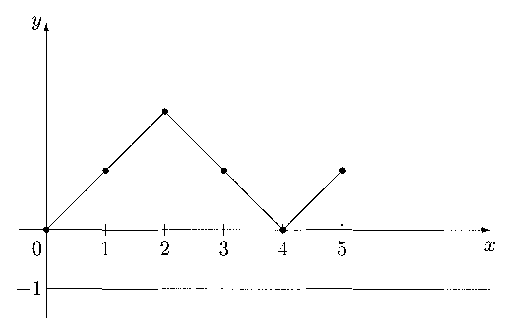
\includegraphics{chap01-vend-scan-01.eps}
\end{figure}



\subsection{}\label{ch01:sec1C}
The modular figure\index{modular figure} was almost certainly known to Gauss\index{Gauss}, probably through his researches on quadratic forms\index{modular group!and quadratic forms}. Let $Q$ be a positive definite binary form with real coefficients:
\begin{equation*}
Q(x, y)=\alpha x^{2}+2\beta xy\,+\gamma y^{2},\qquad\alpha>0,\qquad \Delta=\alpha\gamma-\beta^{2}>0.
\end{equation*}
If $Q(x, y)=n$ for some \emph{integers} $x,\,y$, we say $Q$ \emph{represents} $n$. Let $V$ be a linear homogeneons transformation \eqref{ch01:eqn5} with integral coefficients and determinant $ad-bc=\pm 1$. Then $x=Vx^{\prime},\,y=Vy^{\prime}$ can be solved in integers $x^{\prime},\,y^{\prime}$; hence $Q(x, y)=Q(Vx^{\prime}, Vy^{\prime})=Q^{\prime}(x^{\prime}, y^{\prime})$ also represents $n$, and conversely. We call $Q$ and $Q^{\prime}$ \emph{equivalent}. Thus equivalent forms represent the same integers. Since equivalent forms also have the same discriminant\footnote{$\Delta^{\prime}= \det Q^{\prime}=\det V^{\prime}Q V=\det Q = \Delta$, since $\det V= \pm 1$.} $\Delta$, we may consider, for the problem of representation, only forms having a given discriminant.

We now represent $Q$ by a unique point $\tau$ in $\mathscr{H}$, namely,
\begin{equation*}\tag{$^{\ast}$}
\tau =\frac{x}{y}=(-\beta+i\Delta^{1/2})/\alpha,
\end{equation*}
the solution of $y^{-2}Q(x/y, 1)=0$. Conversely, a point $\tau =u+iv\in \mathscr{H}$ is the representative of the unique form $Q$ with
\begin{equation*}
\alpha v=\Delta^{1/2},\qquad \beta v=-u\Delta^{1/2},\qquad \gamma v=(u^{2}+v^{2})\Delta^{1/2}
\end{equation*}
as a small calculation shows. The points of $\mathscr{H}$ are in 1-1 correspondence with the set of $Q$ of discriminant $\Delta$. In the definition of equivalence of $Q$ we may now suppose $ad-bc=1$, since $\tau$ is always in $\mathscr{H}$.

Notice, moreover, that equivalent $Q$ have representatives $\tau$ that are equivalent under the modular group. For if $Q$ is represented by $\tau,\,Q^{\prime}$ is represented by
\begin{equation*}
x^{\prime}/y^{\prime}=V_{x}/V_{y}=(ax +by)/(cx+dy)=(a\tau +b)/(c\tau+d) =\overline{V}\tau.
\end{equation*}

We use the equivalence relation defined in $\{Q\}$ to partition it into disjoint \emph{equivalence classes}: all the forms in one class represent the same integers, and different classes represent different integers. The different equivalence classes now correspond to inequivalent points $\tau$, and a  complete set of such points constitute a fundamental region $R$. If we use for $R$ the region \eqref{ch01:eqn14}, we can translate the inequalities back to the coefficients $Q$ by $(^{\ast})$; we then find the conditions
\begin{equation}\label{ch01:eqn15}
 -\alpha\leqq 2\beta\leqq\alpha<\gamma \quad \mbox{or}\quad 0\leqq 2\beta\leqq\alpha=\gamma.
\end{equation}
A form satisfying either inequality is said to be \emph{reduced. Every form} $Q$ \emph{of given discriminant} $\Delta$ \emph{is equivalent to exactly one reduced form}, or, to put it another way, \emph{the region} $R$ \emph{represents a complete set of inequivalent forms} $Q$ \emph{of
discriminant} $\Delta$.


\subsection{}\label{ch01:sec1D}
The elliptic functions were discovered about 1825; the elliptic modular invariant $J$, in 1877. This does not mean that it took 50 years for mathematicians to shift the emphasis from argument to parameter in the elliptic function. What happened was this.

The elliptic functions were first found by inverting \emph{elliptic integrals}. In the Legendre\index{Legendre} form, which was standard at the time, a typical integral would be
\begin{equation}\label{ch01:eqn16}
w=E(z)=\int_{0}^{z}\{(1-t^{2})(1-k^{2}t^{2})\}^{-1/2}dt;
\end{equation}
$k$ is a parameter. By inversion of the integral we obtain a function $z=\varphi(w)$ which can be shown to be single-valued. The integral $E(z)$ is not single-valued; its value depends on the path connecting $0$ and $z$. The paths must be considered on a Riemann surface on which the integrand becomes single-valued, and such a surface is conformally equivalent to a torus. This shows there are two independent closed paths (cycles), corresponding to the meridians and circles of latitude on the torus. The ambiguity in $E(z)$ depends linearly, with integral coefficients, on the value of the integral over the cycles. In the inversion the \emph{ambiguities} of the integral $E$ become \emph{periods} of the inverse function $\varphi$, which is therefore an elliptic function in the sense of our definition in \ref{ch01:sec1A}.

The quantity $k^{2}$ was called the \emph{modulus}. It is a function of the ratio of the periods. It is $k^{2}$ that was considered the fundamental function by Abel\index{Abel}, Jacobi\index{Jacobi}, and their followers (especially Hermite\index{Hermite}), and they made exhaustive investigations of its properties. Nowadays we think of $J$ as the basic function.

In the Eisenstein-Weierstrass\index{Eisenstein}\index{Weierstrass} notation $k^{2}$ is written $\lambda$ and appears as (cf. \eqref{ch01:eqn13})
\begin{equation}\label{ch01:eqn17}
\lambda(\tau)=\frac{e_{2}(\tau)-e_{3}(\tau)}{e_{1}(\tau)-e_{3}(\tau)}.
\end{equation}
$\lambda$ is regular and zero-free throughout $\mathscr{H}$, since the $\{e_{i}\}$ are regular and unequal. Let us now investigate the behavior of $\lambda$ under modular transformations.

Notice that if $V\in\overline{M}$, then
\begin{equation*}
\frac{\tau^{\prime}}{2}=\frac{1}{2}\,V\tau=\frac{a(\tau/2)+b/2}{2c(\tau/2)+d}
\end{equation*}
is also in $\overline{M}$ provided $b$ and $c$ are even, which forces $a$ and $d$ to be odd. That is,
\begin{equation*}
V\equiv I\,(\mathrm{mod}\, 2),
\end{equation*}
where $I$ is the identity matrix. Let us denote by $\overline{M}_{1}$ the subgroup of $\overline{M}$ defined by this condition. From the definition \eqref{ch01:eqn1} of $\wp$ we read off
\begin{equation*}
\wp\bigg(\frac{W\tau}{2}|W\tau, 1\bigg)=(c\tau +d)^{2}\wp\bigg(a\,\frac{\tau}{2}+\frac{b}{2} |\,\tau,\, 1\bigg),\quad W=\left(\begin{matrix}
a & b\\ c & d
\end{matrix}\right)
\end{equation*}
for $W\in M_{1}$. Now $a(\tau/2)+b/2$ differs from $\tau/2$ by $m\tau +n$ with $m,\,n$ integral. Hence the right member equals $\wp(\tau/2\,|\,\tau, 1)$. That is,
\begin{equation*}
e_{1}(W\tau)=(c\tau\,+d)^{2}e_{1}(\tau),\quad W\in M_{1}
\end{equation*}
and $e_{2},e_{3}$, satisfy the same equation. \emph{It follows that} $\lambda(\tau)$\index{$\lambda(\tau)$} \emph{is invariant under the subgroup} $M_{1}$.

But is $\lambda$ invariant on a larger subgroup than $M_{1}$? A system of representatives of the cosets of $M_{1}$ in $M$ is:
\begin{equation}
\label{ch01:eqn18} \left(\begin{matrix}
1 & 0\\ 0 & 1
\end{matrix}\right),\quad \left(\begin{matrix}
1 & 1\\ 0 & 1
\end{matrix}\right),\quad\left(\begin{matrix}
1 & 0\\ 1 & 1
\end{matrix}\right),\quad\left(\begin{array}{lr}
1 & -1\\ 1 & 0
\end{array}\right),\quad \left(\begin{array}{lr}
0 & -1\\ 1 & 0
\end{array}\right),\quad\left(\begin{array}{lr}
0 & -1\\ 1 & 1
\end{array}\right).
\end{equation}
Let us consider the last of these: $\tau^{\prime}=-1/(\tau+1)$. From \eqref{ch01:eqn1} we get
\begin{equation*}
\wp\bigg(\frac{\tau^{\prime}}{2}|\,\tau^{\prime}, 1\bigg)=(\tau +1)^{2}\wp\bigg(\frac{1}{2}|\,\tau, 1\bigg),
\end{equation*}
i.e., $e_{1}(\tau^{\prime})=e_{2}$. Likewise $e_{2}(\tau^{\prime})=e_{3},\, e_{3}(\tau^{\prime})=e_{1}$. Hence
\begin{equation*}
\lambda(-1/(\tau+1))=\frac{e_{3}-e_{1}}{e_{2}-e_{1}}=1\bigg/\bigg(1-\frac{e_{2}-e_{3}}{e_{1}-e_{3}}\bigg)=1/(1-\lambda).
\end{equation*}
Similarly, the remaining transformations of \eqref{ch01:eqn18} map $\lambda$ into $\lambda,\, 1-\lambda,\, \lambda/(\lambda-1), (\lambda-1)/\lambda,\, 1/\lambda$, in the order given. Thus the exact invariance group of $\lambda$ is $M_{1}$. The transformations \eqref{ch01:eqn18} form a group isomorphic to the factor group $M/M_{1}$; it is obviously the symmetric group on the 3 letters $e_{1},\,e_{2},\,e_{3}$.

Abel\index{Abel} and Jacobi\index{Jacobi} were also much occupied with the so-called \emph{transformation of elliptic functions}, that is, the connection between $\lambda(\tau)$ and $\lambda^{\prime}=\lambda(n\tau)$, $n$ being an integer. The transition $\tau \rightarrow n\tau$ is a special case of a \emph{transformation of order} $n$. They proved that $\lambda$ and $\lambda^{\prime}$ are algebraically dependent and succeeded in working out the algebraic equations, called \emph{modular equations}, for a few values of $n$. Let
\begin{equation*}
u=\lambda^{1/8}(\tau),\qquad v=(\lambda^{\prime}(\tau))^{1/8}=u(n\tau).
\end{equation*}
For $n=5$ the modular equation is
\begin{equation}\label{ch01:eqn19}
u^{6}-v^{6}+5u^{2}v^{2}(n^{2}-v^{2})+4uv(1-u^{4}v^{4})=0.
\end{equation}
We observe that this equation, which is known to be irreducible, is of degree one higher than the order. The coefficients are rational integers. For a fixed $u=u_{0}$, and consequently a fixed $\tau$, the roots of \eqref{ch01:eqn19} are
\begin{equation}
\label{ch01:eqn20} v_{j}=n((\tau+16j)/5),\quad j=0,1,\,\cdots,\,4;\qquad v_{\infty}=u(5\tau).
\end{equation}
The left member of \eqref{ch01:eqn19} is invariant under the mapping $u\rightarrow v,\,v\rightarrow-u$.


\subsection{}\label{ch01:sec1E}
The relation of $J$ to $\lambda$, as well as many other isolated facts that had accumulated by 1875, were put in order by Klein's\index{Klein, F.|(} invention of the \emph{Stufentheorie} ([\ref{Klein1}, p. 169ff]). Following Rademacher\index{Rademacher} we shall translate \emph{Stufe}\index{Stufe} as ``level.'' Denote by $\Gamma(n)$ the subgroup of $M$ consisting of all modular matrices $V$ satisfying\footnote{The condition $V\equiv\pm\, I$ in the matrix group corresponds to $V\equiv I$ in the group of linear transformations.}
\begin{equation*}
V\equiv\pm\, I\,(\mathrm{mod}\, n);
\end{equation*}
this is a normal subgroup and is called the principal congruence subgroup\index{principal congruence subgroup} of order $n$. In this notation we now write $M=\Gamma(1)$, $M_{1}=\Gamma(2)$.
A \emph{congruence subgroup of level} $n$ is any subgroup $\Gamma$ of $\Gamma(1)$ such that \footnote{This is equivalent to Klein's original definition. Cf. \ref{ch07:chap07}.
Ex. 6-3.}
\begin{equation}\label{ch01:eqn21}
\Gamma(n)\subset \Gamma \subset \Gamma(1).
\end{equation}
The modular functions or modular forms invariant with respect to $\Gamma$ are said to be \emph{functions} or \emph{forms of level} $n$. Thus $J$ is a function of level 1; $\lambda$, a function of level 2. Of course $J$ is also a function of every level and $\lambda$ of every even level.

It is a fundamental theorem that two modular functions belonging to the same group satisfy an algebraic equation, just as in the case of elliptic functions. Hence two modular functions of the same level $n$ are algebraically dependent, for both are invariant on $\Gamma(n)$. For example, $J=J(\tau)$ and $J^{\prime}(\tau)=J(n\tau)$ are both of level $n$. In fact, writing
\begin{equation*}
n\tau^{\prime}=n\,\frac{a\tau+b}{c\tau+d}=\frac{a(n\tau)+nb}{(c/n)(n\tau)+d},
\end{equation*}
we see that $J^{\prime}(\tau)$ is invariant on the group $\Gamma_{0}(n)$ defined by
\begin{equation*}
\Gamma_{0}(n)=\{V\in\Gamma(1)\,|\,c\equiv 0\quad (\mathrm{mod}\, n)\}.
\end{equation*}
When $n=p$ is a prime, it can be shown that $\Gamma_{0}(p)$ is of index $p+1$ in $\Gamma(1)$. The fundamental region $R_{p}$ of $\Gamma_{0}(p)$ thus consists of $p+1$ copies of that for $\Gamma(1)$, and so $J$ is $(p+1)$-valent in $R_{p}$. Hence in the irreducible equation
\begin{equation}
\label{ch01:eqn22} P(J,\,J^{\prime})=0
\end{equation}
the degree of $J^{\prime}$ must be $p+1$. Observe further
\begin{equation*}
J^{\prime}(-1/p\tau)=J,\qquad J(-1/p\tau)=J^{\prime}.
\end{equation*}
Replacing $\tau$ by $-1/\tau$ in \eqref{ch01:eqn22} therefore yields $P(J^{\prime}, J)=0$. Because of the irreducibility we have $P(J, J^{\prime})=cP(J^{\prime}, J)$ and it is not hard to show the constant $c$ is 1. \emph{Thus} $P$ \emph{is symmetric in} $J$ \emph{and} $J^{\prime}$ and so $P$ has degree $p+1$ in $J$ also.

Klein called \eqref{ch01:eqn22} a modular equation of level 1 and order $p$;
\eqref{ch01:eqn19} is of order 5 and level 16 (because $\lambda^{1/8}$ is of level $16)$. The proof that there is an equation of the form \eqref{ch01:eqn19}, aside from the numerical values of the coefficients, is more complicated than the above argument for the equation \eqref{ch01:eqn22}. Because of the higher level of the functions in \eqref{ch01:eqn19} we have to deal with subgroups of high index in $\Gamma(1)$. But the coefficients of \eqref{ch01:eqn19} are much smaller than those of \eqref{ch01:eqn22}!

If we extend the term ``modular equation'' to any irreducible algebraic equation connecting two modular functions, we can include the famous one connecting $J$ and $\lambda$:
\begin{equation}
\label{ch01:eqn23} J=\frac{4}{27}\frac{(1-\lambda+\lambda^{2})^{3}}{\lambda^{2}(1-\lambda)^{2}}.
\end{equation}
The degree of $\lambda$\index{$\lambda(\tau)$} in this equation comes from the fact that $\Gamma(2)$ is of index 6 in the full group, as we noted in \eqref{ch01:eqn18}.

Klein's way of looking at the modular equation exhibits it clearly as a reflection of the relation to each other of two congruence subgroups. Results of the same completeness and elegance for general discontinuous groups are still lacking.


\subsection{}\label{ch01:sec1F}
Modular equations were used by \citeauthor{Hermite0000}~[\ref{Hermite1}]\index{Hermite}, Kronecker\index{Kronecker}, and Brioschi\index{Brioschi} to obtain the transcendental solution of the general algebraic equation of the fifth degree. For this purpose we recall that elementary algebraic processes are sufficient to reduce the equation of fifth degree to the form
\begin{equation}\label{ch01:eqn24}
t^{5}-t-A =0,
\end{equation}
depending on \emph{one} parameter. On the other hand, the modular equation \eqref{ch01:eqn19} also depends on one parameter, namely $u$, and its roots are known: they are given by \eqref{ch01:eqn20}. Of course \eqref{ch01:eqn19} is of the sixth degree, but Galois\index{Galois} had already proved that it possesses a ``resolvent'' of degree 5. Hermite actually calculated the resolvent; it is the equation satisfied by
\begin{equation}
\label{ch01:eqn25} y=(v_{\infty}-v_{0})(v_{1}-v_{4})(v_{2},-v_{3}),
\end{equation}
namely:
\begin{equation}
\label{ch01:eqn26} y^{5}-2^{4}\cdot5^{3}\cdot u^{4}(1-u^{8})^{2}y - 2^{6}\cdot
5^{1/2}u^{3}(1-u^{8})^{2}(1+u^{8})=0.
\end{equation}
We have now only to match \eqref{ch01:eqn26} with \eqref{ch01:eqn24}.

This is done by the substitution
\begin{equation}
\label{ch01:eqn27} y= 2\cdot 5^{3/4}u(1 - u^{8})^{1/2}t.
\end{equation}
and we find
\begin{equation*}
A=2\cdot5^{-5/4}(1+u^{8}) u^{-2}(1-u^{8})^{-1/2}.
\end{equation*}
Since this is a reciprocal equation of degree 8 in $u^{2}$, we can solve for $u$. The solutions of \eqref{ch01:eqn19} for this value of $u$ are the values $v$ given by \eqref{ch01:eqn20}, and from them we can calculate $y$
from \eqref{ch01:eqn25} and eventually $t$ from \eqref{ch01:eqn27}. Thus the roots of \eqref{ch01:eqn24} are represented by the values of a certain modular function\index{quintic solved by modular function}.

Klein\index{Klein, F.|)} also studied the equation of fifth degree but only as one aspect of a comprehensive and many-sided program. Klein was a geometer by training, a student of Pl\"{u}cker\index{Pl\"{u}cker}, and as a young man of 23 he announced his conviction that geometry is the study of those properties of spaces that are unaltered under the transformations of a group; the different geometries are distinguished by the particular space and the particular group acting on it (Erlangen Program, 1872). He first investigated the group of symmetries of a regular solid, a finite group. Such a group may be visualized first as a group of rotations of a sphere in which the solid is inscribed and then, by stereographic projection, as a group of linear transformations of the plane. Klein found that the groups of the regular solids\index{group of the regular solids} constituted \emph{all} the finite groups of linear transformations except the cyclic group, provided we admit an ideal figure called the \emph{dihedron}, which is a regular polygon of $n$ sides regarded as a solid of zero volume. The cube and octahedron have isomorphic groups of rotations; also the dodecahedron and icosahedron.

The icosahedron group has 60 elements; denote it by $G_{60}$ and its elements by $V_{i}$. If $R(z)$ is a rational function, clearly
\begin{equation*}
w=H(z)=\sum\limits_{i=1}^{60}R(V_{i}\,z)
\end{equation*}
is an automorphic function on the group. Consider the inverse function $z =H^{-1}(w);\,z$ is an algebraic function of $w$ and satisfies a polynomial equation $F(z, w)=0$. This equation is called the icosahedral equation. It has the property that for fixed $w$ the roots $z_{i}$ are known linear transformations of each other. Klein showed that every algebraic equation having this same property is essentially the equation of some finite group. This is the class of equations coming within the purview of his method. By taking resolvents he was able to include in this class the general algebraic equation of degree 2 to 5. How he did this is too involved to be presented here; the reader must be referred to Klein's classic treatise on the icosahedron [\ref{Klein2}]\footnote{Cf. also an excellent review of Klein's book by \citeauthor{Cole0000}~[\ref{Cole1}]\index{Cole, F.N.}.} For Klein the important thing was to connect the study of an algebraic equation with other parts of mathematics such as group theory, differential equations (cf. \ref{ch01:sec1G}), and geometry; the expression of the roots by means of some transcendental function was almost incidental.


\subsection{}\label{ch01:sec1G}
We now turn to a quite different line of development. In the theory of differential equations\index{differential equations} the following problem was investigated by \citeauthor{Schwarz0000}~[\ref{Schwarz1}]\index{Schwarz, H. A.} in 1872, following work of \citeauthor{Kummer0000}~[\ref{Kummer1}]\index{Kummer} in 1836 and \citeauthor{Riemann0000}~[\ref{Riemann1}]\index{Riemann} in 1857: \emph{to find all cases of the hypergeometric differential equation}
\begin{align}\label{ch01:eqn28}
\frac{d^{2}\eta}{dw}+p_{1}(w)\frac{d\eta}{dw}+p_{2}(w)\eta=0,\qquad & p_{1}=\frac{(\alpha+\beta+1)w-\gamma}{w(w-1)},\\
&p_{2}=\frac{\alpha\beta}{w(w-1)}\nonumber
\end{align}
\emph{which can be integrated by algebraic functions of} $w$. (This equation has as one solution the hypergeometric function $F(\alpha, \beta, \gamma;w)$ of Euler\index{Euler} an Gauss\index{Gauss}.) Later there was discovered in the files at G\"{o}ttingen a ``Vorlesung'' of Riemann,\index{Riemann} 1858/9, that contained most of Schwarz's\index{Schwarz, H. A.} results; this was not published until 1902 (\citeauthor{Riemann0000}~[\ref{Riemann2}], Nachtr\"{a}ge. pp. 69--93]).

Let $\eta_{i}(w),\, i=1,2,$ be a system of fundamental solutions of \eqref{ch01:eqn28} which are regular at $w =w_{0}$, a point distinct from the singular points $0, 1,\infty$, and let
\begin{equation*}
z(w)=\eta_{1}(w)/\eta_{2}(w).
\end{equation*}
On continuing $z$ analytically around a closed curve in the $w$-plane, the solutions $\eta_{i}$ remain solutions but may not return to their initial values. But since any solution is a linear combination of $\eta_{1}$ and $\eta_{2}$, we see that the final value of $z$ is
\begin{equation*}
z_{1}=\frac{a\eta_{1}+b\eta_{2}}{c\eta_{1}+d\eta_{2}}=\frac{az+b}{cz+d}.
\end{equation*}
\emph{The quotient of two solutions of} \eqref{ch01:eqn28} \emph{has undergone
a linear transformation} (which may be the identity) as $w$ traverses a closed curve. The set of all linear transformations arising from all possible circuits is obviously a group, called the \emph{monodromy group}\index{triangle group} of the differential equation. Denote it by $\Gamma$. Writing
\begin{equation*}
z=\zeta(w), \qquad w=f(z)
\end{equation*}
we now have that
\begin{equation*}
w=f(z)=f(Vz)
\end{equation*}
for each transformation $V$ in $\Gamma$. In other words, $f$ is an automorphic function\index{automorphic function} with respect to $\Gamma$.

Schwarz next obtained a differential equation of third order satisfied by $z$:
\begin{equation*}
\frac{z^{\prime\prime\prime}}{z^{\prime}}-\frac{3}{2}\bigg(\frac{z^{\prime\prime}}{z^{\prime}}\bigg)^{2}=\frac{1-\lambda^{2}}{2w^{2}}+\frac{1-\mu^{2}}{2(1-w)^{2}}+\frac{\lambda^{2}+\mu^{2}-\nu^{2}-1}{2w(w-1)},
\end{equation*}
where $\lambda=1-\gamma,\,\mu =\gamma-\alpha-\beta,\, \nu=\beta-\alpha$. The left member of the equation is the \emph{Schwarzian derivative}\index{Schwarzian derivative}, which is invariant when $z$ is subjected to a linear transformation. He showed that for real $\lambda,\,\mu,\,\nu$, the function $z=\zeta(w)$ maps the upper half of the $w$-plane conformally and 1-1 onto a triangle with angles $\lambda\pi,\,\mu\pi,\, \nu\pi$ bounded by circular arcs or line segments (cf. Figure). This is an elegant solution to an important mapping problem.

Since we want $\eta$ to be algebraic in $w$, we must also have $z$ algebraic in $w$. Then the inverse function $w=f(z)$ will be single-valued in the neighborhood of all except branch points. By standard devices from the theory of differential equations one can show from \eqref{ch01:eqn28} that $\lambda,\mu,\nu$ \emph{must be either} 0 \emph{or the reciprocal of a positive integer}.

We now continue $z$ analytically by the Riemann-Schwarz reflection principle\index{Riemann-Schwarz reflection principle}. The original triangle is shaded, as is the upper half-plane. Now reflect in the side $c$, which is equivalent to extending $z$ into the lower half-plane across the segment $(1, \infty)$. Next, we can reflect in the side $b$, which means we cross the segment $(0, 1)$, or in the side $a$, corresponding to the segment $(-\infty, 0)$. The new triangle is left unshaded, as is the lower half-plane.

We continue the process indefinitely, always reflecting in a free side of the figure in the $z$-plane. Since reflection is a conformal mapping, all triangles thus obtained will have the same angles $\lambda\pi,\,\mu\pi,\,\nu
\pi$. Furthermore, because of the condition on $\lambda,\,\mu,\,\nu$, there will be no overlapping of triangles. The plane, or a portion of the plane, is covered without gaps and without overlapping by a network of triangles.

Let $w$ be a point in the upper half-plane; then $z$ will lie in a shaded triangle.

\begin{figure}[!h]
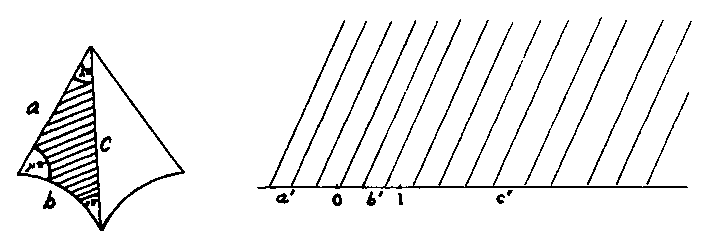
\includegraphics{chap01-vend-scan-02.eps}
\end{figure}

\noindent The performance of two reflections leaves $w$ unaltered but carries $z$ into another shaded triangle. Similarly for points in the lower half-plane, which correspond to points in an unshaded triangle. Thus the same point $w$ corresponds to points $z$ which are carried into each other by an even number of reflections. That is, $w=f(z)$ is automorphic with respect to the group consisting of all products of an even number of reflections. The group is called a triangle group and $f$ a triangle function. The union of a shaded and unshaded triangle is a fundamental region for the group. Since the group has a fundamental region, it is discontinuous.

There are 3 markedly different cases depending on the value of $\lambda+\mu+\nu$
(cf. [\citeauthor{Ford0000}~\ref{Ford1}\index{Ford}, pp. 306--308]). If $\lambda+\mu+\nu =1$, we have a straight-sided triangle. There are only 4 possibilities, including a degenerate one $(\lambda, \mu, \nu)= (1/2, 1/2, 0)$---a half-strip. The finite plane is covered by the network of triangles. The groups are related to the simply and doubly periodic groups; They contain only elliptic and parabolic transformations.

If $\lambda+\mu+\nu>1$, we can map the trianglkes stereographically on the sphere and obtain a covering with a finite number of triangles. The groups are thus finite; they are the groups of symmetries of the regular solids mentioned in IF.

The remaining case, $\lambda+\mu+\nu<1$, is the most interesting for us (cf. \ref{ch07:chap07}. \ref{ch07:sec1G}). Let the mapping be normalized so that two sides of the triangle are straight. Because the angle sum is less than $\pi$, the third side $BC$ is convex toward $A$ (cf. Figure). Draw a line $AM$ tangent to the circle $BC$. The circle $\mathscr{Q}$ with center $A$ and radius $AM$ is orthogonal to the three sides of triangle $ABC$. A reflection in any side of the triangle leaves $\mathscr{Q}$ fixed. The new triangle will have its sides orthogonal to $\mathscr{Q}$, and so on. Thus the reflection process leads to an infinite network of nonoverlapping triangles all lying within $\mathscr{Q}$. It can be shown that these triangles fill the interior of $\mathscr{Q}$. The figure on page 15 is drawn for the case (1/2, 1/3, 1/7).

\begin{figure}[!h]
\includegraphics{chap01-vend-scan-03.eps}
\end{figure}

The modular group is included among the triangle groups; it is the case (1/3, 1/2, 0). The vertex of angle 0 is of course on $\mathscr{Q}$. The principal congruence group $\Gamma(2)$ is also included; it is (0, 0, 0). Cf. Figures, p. 16. Incidentally, Dedekind\index{Dedekind} developed the modular function $J$ by this reflection process.

We have seen that the stated conditions on $\lambda,\,\mu,\,\nu$ are necessary in order that in \eqref{ch01:eqn28} $\eta$ be an algebraic function of $w$. But if $\eta$ is algebraic in $w$, so is $z$. Then to each $w$ there corresponds only a finite number of $z$. But to each $w$ there correspond all the transformations $Vz$ belonging to the triangle group. Hence the triangle group must be finite, and clearly this condition is also sufficient. \emph{That is, in the differential equation} \eqref{ch01:eqn28} $\eta$ \emph{is an algebraic function of} $z$ \emph{if and only if} $1/\lambda,\, 1/\mu,\,1/\nu$ \emph{are integers and} $\lambda+\mu+\nu>1$, \emph{or equivalently, if and only if} $w=f(z)$ \emph{is an automorphic function with respect to a finite group}. This is the solution of the problem announced at the beginning of this subsection.


\begin{figure}[h]
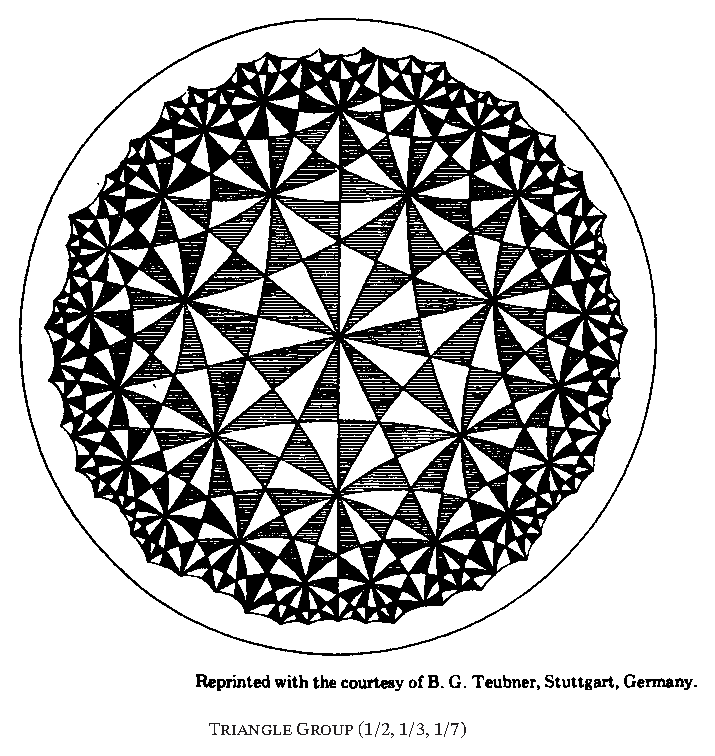
\includegraphics{chap01-vend-scan-04.eps}
\end{figure}

We have seen that Schwarz had automorphic functions that go beyond the modular functions. Klein\index{Klein, F.} was well aware of Schwarz's\index{Schwarz, H. A.} work and extended it in special cases to polygons of more than 3 sides. However, by the reflection process one can obtain only fundamental regions of certain geometrical types and it was left to Poincar\'{e}\index{Poincar\'{e}} to discover the form of the general fundamental region (cf. Section~\ref{ch01:sec2}).

\begin{figure}[h]
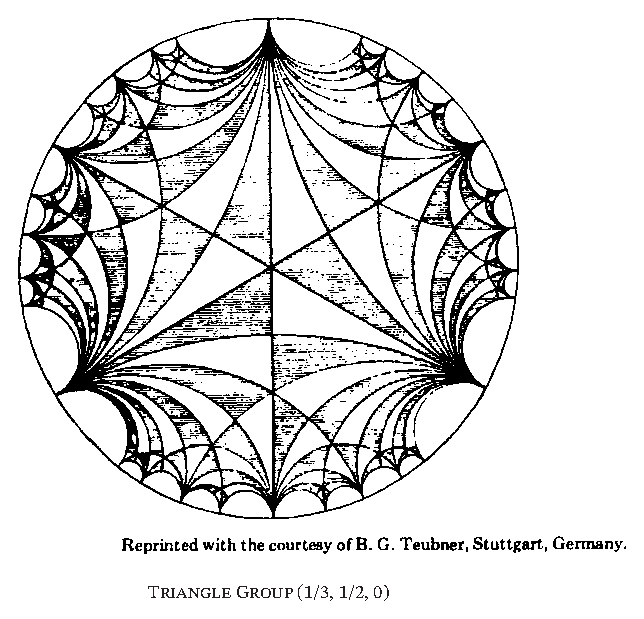
\includegraphics{chap01-vend-scan-05.eps}
\end{figure}

\begin{figure}[h]
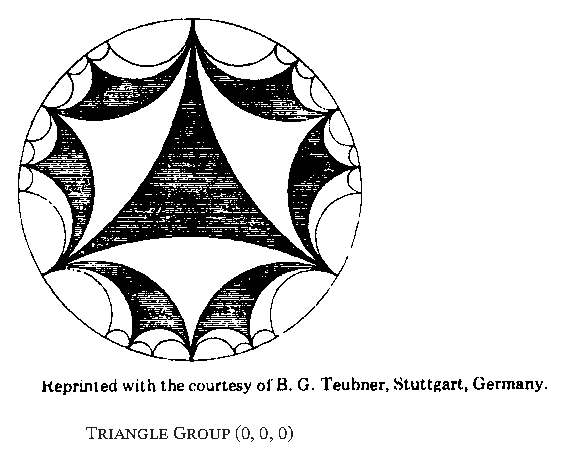
\includegraphics{chap01-vend-scan-06.eps}
\end{figure}


\subsection{}\label{ch01:sec1H}
No discussion of elliptic functions, however brief, can omit mention of the \emph{theta functions}\index{theta function}, those remarkable transcendents known in special cases to Euler\index{Euler} and Gauss\index{Gauss} but only completely and systematically explored by Jacobi\index{Jacobi} in his great work \emph{Fundamenta Nova} [\ref{Jacobi}].

There are 4 theta functions:
\begin{equation}\label{ch01:eqn29}
\begin{split}
\vartheta_{1}(z|\tau)&=-i\textstyle\sum\,(-1)^{n}q^{(n+1/2)^{2}}e^{(2n+1)\pi
i z},\\
\vartheta_{2}(z|\tau)&=\textstyle\sum\,q^{(n+1/2)^{2}}e^{(2n+1)\pi iz},\\
\vartheta_{3}(z|\tau)&=\textstyle\sum q^{n^{2}}e^{2\pi inz},\\
\vartheta_{4}(z|\tau)&=\textstyle\sum\,(-1)^{n}q^{n^{2}}e^{2\pi inz}
\end{split}
\end{equation}
where $q=e^{\pi i\tau}$ and all series run over all integer values of $n$. It is seen that each theta is an \emph{entire} function of $z$ and is \emph{regular} for $|q|<1$, i.e., $\mathrm{Im}\, \tau>0$. A remarkable feature of these functions is that they also have product representations, for example,
\begin{equation}\label{ch01:eqn30}
\vartheta_{3}(z\,|\,\tau) =\prod_{1}^{\infty}\,(1-q^{2n})(1+q^{2n-1}e^{2\pi
iz})(1+q^{2n-1}e^{-2\pi iz}).
\end{equation}
The equality of the two representations leads to some famous identities, of which the following one, due to Euler, may be mentioned:
\begin{equation}\label{ch01:eqn31}
\sum\limits_{n=-\infty}^{\infty}(-1)^{n}q^{n(3n+1)}=\prod_{1}^{\infty}(1-q^{2n}).
\end{equation}
There are many remarkable identities involving theta functions; their study is a subject in itself.

The theta functions provide a solution to an important problem: to represent an elliptic function, which is \emph{meromorphic}, by the quotient of two \emph{entire} functions. For example, the function $sn(u, k)$, which is the inverse of the elliptic integral \eqref{ch01:eqn16}, is given by
\begin{equation*}
sn(u,\,k)=\frac{1}{\sqrt{k}}\frac{\vartheta_{1}(u/2K|\,\tau)}{\vartheta_{4}(u/2K|\,\tau)},\qquad \tau=iK^{\prime}/K
\end{equation*}
where $2K,\,4iK^{\prime}$ are the periods of $sn(u),\,K$ being the real period.

The theta functions have transformation properties in the parameter $\tau$.
Thus\footnote{Define $\tau^{1/2}$ so that $(-i\tau)^{1/2}$ is positive for $\tau$ purely imaginary.}:
\begin{equation*}
\vartheta_{3}(z\,|\,\tau+2)=\vartheta_{3}(z\,|\,\tau),\qquad \vartheta_{3}(z/\tau\,|-1/\tau)=(-i\tau)^{1/2}e^{\pi it^{2}/\tau}\vartheta_{3}(z\,|\,\tau)
\end{equation*}
and for $z=0$ this is $(\vartheta_{3}(\tau)=\vartheta_{3}(0\,|\,\tau))$:
\begin{equation}
\label{ch01:eqn32} \vartheta_{3}(\tau+2)=\vartheta_{3}(\tau),\qquad \vartheta_{3}(-1/\tau)=(-i\tau)^{1/2}\vartheta_{3}(\tau).
\end{equation}
(The second formula is a famous exercise in texts on function theory.) We see that $\vartheta_{3}$ behaves almost like a modular form of dimension $-1/2$ on the group $\Gamma$ generated by $\tau \rightarrow \tau+2,\tau\rightarrow-1/\tau$. But it picks up a \emph{multiplier}, $i^{-1/2}$, under the latter transformation. We are therefore led to consider more general modular forms belonging to a class $\{\Gamma, -r, v\}$\index{$\{\Gamma, -r, v\}$}, where $\Gamma$ is the group, $-r$ is the dimension, and $v$ is a \emph{multiplier system}\index{multiplier system}. That is, $v$ is a function of the elements of $\Gamma$. Moreover, $v(M_{1}M_{2})$ can be calculated from $v(M_{1})$ and $v(M_{2})$. From the fact that $|v|=1$ on the generators of $\Gamma$ we can deduce that $|v|=1$ always. Thus $v$ is a mapping from $\Gamma$ into the complex numbers of modulus 1. When $r$ is an integer, $v$ is in fact a \emph{character} of the group $\Gamma$.

The $\vartheta_{i}$ can be used for the \emph{problem of inversion}: to express the modulus $k$ in terms of the periods $2K,\,4iK^{\prime}$. Indeed,
\begin{equation*}
k^{1/2}=\vartheta_{2}(\tau)/\vartheta_{3}(\tau),\qquad \tau=iK^{\prime}/K.
\end{equation*}
Thus we can express the parameter $u$ of the modular equation\footnote{Since the theta functions, being infinite products, never vanish, we can extract roots without fear.} \eqref{ch01:eqn19}:
\begin{equation*}
u(\tau)=\lambda^{1/8}=k^{1/4}=\sqrt{2}\,q^{1/8}\frac{\sum\limits_{-\infty}^{\infty}(-1)^{n}q^{n(2n+1)}}{\sum\limits_{-\infty}^{\infty}(-1)^{n}q^{2n^{2}}}\,\cdot
\end{equation*}
Given a value $u=c$, we determine $\tau$ by inverting this series, or rather one closely related to it; this gives a very rapidly converging series for $q=e^{\pi i\tau}$. The roots of \eqref{ch01:eqn19} are then found from \eqref{ch01:eqn20}.

Because of the very rapid convergence of the series \eqref{ch01:eqn29}, the theta functions are useful in all problems of computation. The function $\vartheta_{3}(iy)$, for example, is represented by its first term $2e^{-\pi y/4}$ with an error of less than one percent for $y$ as small as 3/4. If $y$ is much smaller than this, we can use the transformation equation \eqref{ch01:eqn32}, which sends $y$ into $1/y$. Since $y$ is small, $1/y$ is large, and the transformed series converges rapidly.

The theta functions appear out of nowhere. Their place in the general theory is not clear. But such marvelous gifts must he used.


\subsection{}\label{ch01:sec1I}
We have barely mentioned Riemann\index{Riemann}. Without Riemann, however, the theory of automorphic functions could hardly have blossomed as it did in the last twenty years of the century. I believe Riemann's significance for our subject is due to three things.

First, he created a new climate in the theory of analytic functions. The appeal was to general principles rather than to formulas and calculation. For example, functions were characterized by the position and nature of their singularities instead of by a specific representation. The principle of
analytic continuation was introduced and freely used. He advertised the new methods in papers like those on the hypergeometric series, abelian functions, and the zeta function. The power and efficacy of these methods, which not only made possible simpler and more direct proofs but opened up entirely new fields for investigation, must have startled the mathematicians of that day.

Secondly, he invented specific tools which have proved to be essential in the further development of analytic function theory. Above all must be mentioned the conformal mapping theorem which, as we have seen, was used by Schwarz\index{Schwarz, H. A.} to construct the first automorphic functions beyond the elementary cases. It was later to find a deeper application in the theory of uniformization.

Thirdly, Riemann's publications exerted a profound influence on the youthful Klein\index{Klein, F.|(}. The latter built his own program in function theory as the working out of ideas which he felt had already been seen by Riemann\index{Riemann}. It was entirely natural for Klein to use Riemann surfaces as the foundation for his theory of automorphic functions.

Riemann's influence on the shape of things to come cannot be better described than by the following words of Poincar\'{e}\index{Poincar\'{e}|(}:

``Riemann a cr\'{e}\'{e} une th\'{e}orie nouvelle des fonctions, et il sera toujours possible d'y retrouver le germe de tout ce qui s'est fait et se fera apr\'{e}s lui en analyse math\'{e}matique....''


\section{Founding of the Theory of Automorphic Functions}\label{ch01:sec2}

\subsection{}\label{ch01:sec2A}
That was the state of the art when in the spring of 1880 the 26-year-old Poincar\'{e} read a paper of \citeauthor{Fuchs0000}~[\ref{Fuchs1}]\index{Fuchs, L.} and as a result entered into correspondence with him. In the course of this paper Fuchs carried the idea of Schwarz (cf.~\ref{ch01:sec1G}) one step further; he considered linear differential equations of second order with rational coefficients and obtained analogous results. Fuchs' paper had a strong catalytic effect on Poincar\'{e}, who promptly rediscovered the triangle functions (he had not read Schwarz). Soon he generalized the triangle to a polygon with bounding arcs orthogonal to the unit circle, and not unnaturally called the groups which arose, as well as the associated automorphic functions, \emph{Fuchsian}.

By summer Poincar\'{e} was writing an essay on automorphic functions for a competition sponsored by the Paris academy.\footnote{Poincar\'{e}'s paper won honorable mention. The prize went to Halphen\index{Halphen}.} The next year he published no fewer than 11 notes in the \emph{Comptes Rendus}, in which he sketched a theory essentially complete in all important respects. Full details were provided in five long articles appearing in the first issues of the new publication \emph{Acta Mathematica} (1882/4).

It was an amazing performance. Klein soon wrote Poincar\'{e} and their correspondence makes fascinating reading (\citeauthor{Klein0000}~[\ref{Klein1}, 587--621]).


\subsection{}\label{ch01:sec2B}
Poincar\'{e} first investigated those groups of linear transformations of the plane each element of which maps a given disk (or half-plane) on itself\footnote{For a detailed treatment cf. \ref{ch04:chap04}. \ref{ch04:sec7}.}  (\citeauthor{Poincare0000}~[\ref{Poincare1}, pp. 108--168]). The boundary of the invariant disk is called the \emph{principal circle}\index{principal circle}; we may suppose it to be the unit circle $\mathscr{Q}:|z|=1$ with interior $\mathscr{U}$. The automorphic functions, which were the goal of the investigation, would be defined on $\mathscr{U}$ and invariant under the group $\Gamma$:
\begin{equation*}
f(Vz)=f(z)
\end{equation*}
for each linear transformation $V$ belonging to $\Gamma$. Then $\Gamma$ must be \emph{discontinuous}\index{discontinuous group}: the sets\footnote{$\Gamma z=\{V z\,|\,V \in\Gamma\}$.} $\Gamma z,\,z\in\mathscr{U}$, must not have any points of accumulation in the interior of $\mathscr{U}$. Otherwise $f$ would take the same value infinitely often in the neighborhood of an accumulation point $\zeta$ and could not be analytic at $\zeta$ unless it were a constant. Poincar\'{e} showed that $\Gamma$ is discontinuous if and only if it is \emph{discrete} (no sequence of matrices $V_{n}\in \Gamma$ converges to a non-singular matrix). The discontinuous principal-circle groups Poincar\'{e} called \emph{Fuchsian}. Later he added another restriction.

We call two points $\Gamma$-\emph{equivalent} if there is a transformation in $\Gamma$ sending one point into the other. Under this relation the points of $\mathscr{U}$ are partitioned into disjoint classes of mutually equivalent points. A \emph{fundamental set} is a set consisting of exactly one point from each equivalence class.

Let us consider a simpler case: the doubly periodic group generated by the translations $z\rightarrow z+1,\, z\rightarrow z+i$. Obviously a fundamental set for this group can be taken as an open square of unit side together with the points on the western and southern sides (open) and the southwest corner. Call the interior of this fundamental set a \emph{fundamental region}\index{fundamental region}. The images of the fundamental region by transformations of the group are other squares, disjoint from the first square and from each other, the whole forming a paving or \emph{tessellation}\index{tessellation} of the plane.

In the same way we can construct a fundamental region for a Fuchsian group\index{Fuchsian group} $\Gamma$; this, together with its images by elements of $\Gamma$ will divide $\mathscr{U}$ into nonoverlapping regions. However, this partition can hardly be called a tessellation since the regions are of widely varying sizes, the ones near the boundary being much smaller than those near the center.

It was Poincar\'{e}'s great inspiration to recognize that this partitioning of $\mathscr{U}$ may be regarded as a tessellation of the \emph{noneuclidean} plane by a group of \emph{noneuclidean rigid motions}.

The noneuclidean geometry needed is the \emph{hyperbolic} geometry (cf. \ref{ch02:chap02}. \ref{ch02:sec12}). This is obtained from euclidean geometry by postulating that through a point not on a line call be drawn not exactly one, but more than one, line
that does not meet the given line. A model of this geometry had been invented by Cayley\index{Cayley} and Klein\index{Klein, F.|)} in the seventies: the hyperbolic plane was represented on $\mathscr{U}$, straight lines were chords of $\mathscr{Q}$, and a formula for distance and angle satisfying the usual requirements was prescribed.

But in this model the distance-preserving transformations (isometries) were projective transformations in the real coordinates of the plane. Poincar\'{e} saw that by introducing arcs of circles orthogonal to $\mathscr{Q}$ as the straight lines of the geometry, the isometries become the linear transformations that preserve $\mathscr{U}$. Since these are conformal mappings and in consequence preserve euclidean angle measure, there is no reason why we cannot use the latter as the angle measure in the hyperbolic geometry\index{hyperbolic geometry}. We denote the hyperbolic concepts by prefixing $H$; thus, $H$-line. etc.

In the Poincar\'{e} model, then, $\mathscr{U}$ is the $H$-plane, circular arcs orthogonal to $\mathscr{Q}$ are $H$-lines, euclidean angle measure is $H$-angle measure, and $\Gamma$ \emph{may be considered as a group of} $H$-\emph{isometries} (\emph{rigid motions}). We can now easily obtain the desired tessellation of $\mathscr{U}$.

The rigid motions are of three types: \emph{elliptic}, a (hyperbolic) rotation about two fixed points, one inside $\mathscr{U}$, the other inverse to it and so outside $\mathscr{U}$; \emph{hyperbolic}, an $H$-translation with distinct fixed points on $\mathscr{Q}$: and \emph{parabolic} (also called limit-rotation) with a single fixed point on $\mathscr{Q}$. These names are
due to Klein.

It is curious that though Poincar\'{e} was led to the solution of this problem by considerations of noneuclidean geometry (as he himself clearly states in more than one place), he avoids all use of it in his finished presentation. He says he does this to avoid any possibility of confusion. Everyone since Poincar\'{e}, however, has made the proof in terms of hyperbolic, geometry, and we shall, also.


\subsection{}\label{ch01:sec2C}
Let $w_{0}$ be a point of $\mathscr{U}$ that is not fixed by any element of a Fuchsian group\index{generators of Fuchsian group}\index{relations in a group} $\Gamma$. The images $\{w_{i}=V_{i}w_{0}, V_{i}\in \Gamma\}$ are distinct distinct points. Define $N_{0}$ to be the set of points in $\mathscr{U}$ that are nearer to $w_{0}$ (in the hyperbolic\index{hyperbolic geometry} sense) than to any $w_{i}\not=
w_{0}$, or, as we shall to say, strictly nearer $w_{0}$. The image $N_{i}=V_{i}N_{0}$ then consists of the points that are strictly nearer $w_{i}$, for the $H$-distance from $w$ to $w_{0}$ equals the $H$-distance from $V_{i}w$ to $V_{i}w_{0}=w_{i}$ because of the invariance of $H$-distance under the mappings of $\Gamma$.
\emph{Hence the sets} $N_{i}$ \emph{do not overlap}.

Let $K$ be a closed disk lying in $\mathscr{U}$. There are only a finite number of $w_{i}$ lying in $K$, otherwise there would be in $K$ a point of
accumulation of the set $\Gamma w_{0}$, which is ruled out because of the discontinuity of $\Gamma$ in $\mathscr{U}$. Suppose now $z$ is an arbitrary point of $\mathscr{U}$; in a suitable disk about $z$ there must be one of the $w_{i}$, say $w_{k}$, which is as near to $z$ as any other $w_{i}$. Then
$z$ lies in $N_{k}$ or on its boundary. \emph{The set of images of the closure of} $N_{0}$ \emph{by elements of} $\Gamma$ \emph{covers} $\mathscr{U}$.

Here then is our tessellation\index{tessellation} of $\mathscr{U}$. The sets $\{N_{i}\}$ are called
\emph{normal polygons}\index{normal polygon}. They are actually noneuclidean polygons, for it is not hard to establish that the boundary of $N_{i}$ is cut out by the $H$-perpendicular bisectors of the segments $\{w_{i}w_{j},\,j \neq i\}$. The normal polygons are connected, simply connected, and convex. It may happen that the normal polygon has infinitely many sides, in which case the word ``polygon'' must be taken in a generalized sense. However, Poincar\'{e} restricted himself to the case of finitely-sided polygons and so defined the term ``Fuchsian.''

The tessellation may be of two types: in a group of the \emph{first kind}, the normal polygon touches the unit circle $\mathscr{Q}$ at most in points; in a group of the \emph{second kind}, the boundary of the normal polygon contains one or more arcs of $\mathscr{Q}$ called \emph{free sides} (cf. Figure). The tessellation has complete symmetry: a noneuclidean observer sees the same pattern from one point of $\mathscr{U}$ as from any other. Furthermore, the tessellation has a characteristic property of a \emph{triangulation}: each point of $\mathscr{U}$ has a neighborhood that meets only a finite number of polygons.

\begin{figure}[!h]
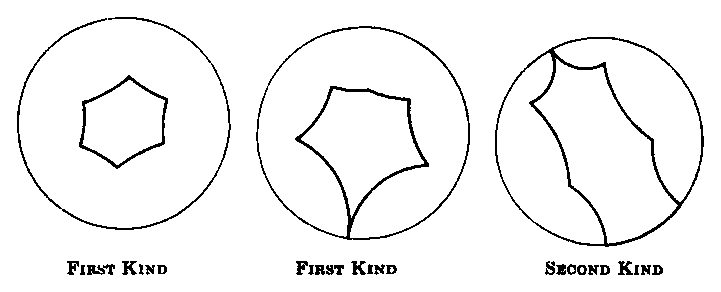
\includegraphics{chap01-vend-scan-07.eps}
\end{figure}

Let $N_{i}$ and $N_{j}$ have a side $s$ in common. There is a $V_{k}\in\Gamma$ that maps $N_{i}$ on $N_{j}$. Then $V_{k}$ must carry some side of $N_{i}$ into $s$. Call this side $s^{\prime}$. We say $s$ and $s^{\prime}$ are \emph{conjugate sides}; they have equal $H$-length. Thus the sides of a normal polygon are arranged in conjugate pairs.\footnote{This does not apply to the free sides.} The number of sides is therefore even. Poincar\'{e} showed, moreover, that \emph{the transformations that pair conjugate sides constitute a set of generators for} $\Gamma$.

A point where two sides of a normal polygon meet is called a \emph{vertex}. Consider the vertices of $N_{0}$, say. A vertex may be equivalent to other vertices; a complete set of equivalent vertices is called a \emph{cycle}. If one vertex of a cycle is a fixed point of some element of $\Gamma$, the same is true of the other vertices; we can therefore speak of \emph{elliptic} and \emph{parabolic} cycles. If no point of a cycle is a fixed point, we call the cycle \emph{accidental}. Every fixed point is a vertex of some normal polygon, but the accidental vertices can be varied by a different choice of the ``center'' $w_{0}$; hence the name ``accidental.'' If $(z_{1}, z_{2},\,\cdots,\, z_{3})$ is an accidental cycle in $N_{0}$, the transformation of the group that send $z_{j}$ to $z_{1}$ send $N_{0}$ into neighboring polygons each having $z_{1}$ as a vertex. The entire neighborhood of $z_{1}$ is covered by these polygons. Since the transformations are conformal mappings, we see that the \emph{sum of the angles at the vertices of an accidental cycle is} $2\pi$. By similar reasoning it is shown that \emph{the sum of the angles at the vertices of an elliptic cycle} is $2\pi/l$, where $l$ is the order of the elliptic transformation fixing one of the points of the cycle. A cycle lying on $\mathscr{Q}$ is either parabolic, or else it consists of two vertices each of which is the intersection of a side and a free side; in the latter case the angle sum is seen to be $\pi$.

Let us draw a small simple closed curve around a vertex $\omega$ in $\mathscr{U}$. The curve crosses the finite number of fundamental regions assembled around $\omega$. As we proceed along the curve, the transition from one fundamental region to the next is made by transformations of $\Gamma$, and since we return to the starting point the product of these transformations must be the identity. Thus we get a \emph{relation} in $\Gamma$. Poincar\'{e} showed that the relations obtained in this way from a complete set of circuits, each enclosing a single vertex, are independent and form a basis for all the relations in $\Gamma$. Cf. \ref{ch07:chap07}.~\ref{ch07:sec2}.

Thus Poincar\'{e} deduced that a Fuchsian group gives rise to a tessellation of the unit disk into noneuclidean polygons with certain properties. $He$ \emph{then reversed the process}: one \emph{starts} with a polygon $P_{0}$ with certain properties. We require first that the sides of $P_{0}$ be circular arcs orthogonal to $\mathscr{Q}$ and be arranged in conjugate pairs of equal $H$-length. There is no group as yet. But there do exist linear transformations ($H$-rigid motions) that send each side into its conjugate side. We can now speak of elliptic cycles, etc. We require secondly that the angles of $P_{0}$ have the properties noted above for normal polygons (sum of the angles at an elliptic cycle is a submultiple of $2\pi$ etc.). Poincar\'{e} proved: \emph{the group} $G$ \emph{generated by the above motions is discontinuous}. Cf. \ref{ch07:chap07}.~\ref{ch07:sec1}.

In fact, the generating motions map $P_{0}$ into polygons that border it along its sides. By means of new motions deduced from the original ones it is possible to fill out the complete neighborhood of a vertex with other polygons. These polygons do not overlap each other or the original polygon because of the conditions on the angle sum at the vertices of a cycle. Thus $P_{0}$ is completely surrounded by a ring of nonoverlapping polygons each of which is the image of $P_{0}$ by a product of generating motions.

We continue in this way, obtaining successively larger rings of nonover-lapping polygons. It can be shown that every element of $G$ maps $P_{0}$ into a polygon lying in some ring. Hence the images of $P_{0}$ by elements of $G$ do not intersect. We must still show that each point lies in the closure of some polygon. Draw a straight line $\lambda$ from a point $A$ in $P_{0}$ to an arbitrary point $B$ of $\mathscr{U}$. $\lambda$ crosses infinitely many polygons, otherwise we could deduce the result at once. If $u_{n}$ is the $H$-length of the segment of $\lambda$ cut off by $P_{n}$, then $u_{n}\rightarrow 0$, for $AB$ is of finite length. It follows that when $n$ is sufficiently large $u_{n}$ is so small that $\lambda$ must subtend one and the same vertex. In other words, infinitely many polygons are assembled around one vertex. This contradicts the construction of the polygons if the vertex is in $\mathscr{U}$; if it is on $\mathscr{Q}$, it is parabolic and then $B$ is on $\mathscr{Q}$, a contradiction.

We have constructed a tessellation of $\mathscr{U}$ consisting of a polygon $P_{0}$ and all its images by elements of a group $G$. Hence $G$ is discontinuous.

In this way Poincar\'{e} proved the existence\index{Fuchsian group!existence of} of Fuchsian groups. In fact his method gives a \emph{parameterization} of such groups.


\subsection{}\label{ch01:sec2D}\footnote{Cf. Chapters~\ref{ch05:chap05} and~\ref{ch08:chap08} for extended treatments.}
Having disposed of the principal questions concerning Fuchsian \emph{groups}, Poincar\'{e} next turned his attention to the Fuchsian \emph{functions} (\citeauthor{Poincare0000}~[\ref{Poincare1}, pp. 169--257]). A Fuchsian function\index{Fuchsian function} with respect to a group $\Gamma$ is a meromorphic function that assumes the same value at points of $\mathscr{U}$ equivalent under $\Gamma$; besides this, it must approach a definite value (which may be infinite) as the variable approaches a parabolic vertex from within a fundamental region. The first problem is whether such functions, apart from constants, exist.

Here Poincar\'{e}\index{Poincar\'{e} series!identical vanishing of} used the analogy with the elliptic modular functions as a guiding principle. The function $g_{2}^{3}/g_{3}^{2}$ is invariant under the modular group (cf.~\ref{ch01:sec1A}). Since $dV/dz=(cz+d)^{-2}$ for the unimodular transformation $Vz=(az+b)/(cz+d)$, we can write $g_{2}$ as \footnote{The constant $c$, easily shown to be $\zeta(4)$, arises because we sum over $V$ in the group. i.e., $c,\, d$ are coprime, whereas in \eqref{ch01:eqn3} we summed over all pairs of integers $(c, d)$.}
\begin{equation*}
g_{2}(z)(dz)^{2}=c\quad\sum\limits_{V\in\Gamma(1)}(d\,Vz)^{2},\qquad c= \mathrm{constant}.
\end{equation*}
Suppose we try this more generally; let $H(z)$ be a rational function and
define
\begin{equation}\label{ch01:eqn33}
F(z)(dz)^{m}= \sum\limits_{V\in \Gamma}\,H(Vz)(dVz)^{m},
\end{equation}
where $m$ is a positive integer and $\Gamma$ is an arbitrary Fuchsian group. Assuming that the series converges and can be rearranged, we now have for $L\in\Gamma$:
\begin{equation}\label{ch01:eqn34}
F(Lz)(dLz)^{m}=\sum\limits_{V\in\Gamma}\,H(V\,Lz)(dV\,Lz)^{m}=\sum\limits_{V\in \Gamma} H(Vz)(d\,Vz)^{m}=F(z)(dz)^{m},
\end{equation}
since, when $V$ runs over $\Gamma$, so does $VL$. The ``\emph{differential}'' $F(z)(dz)^{m}$ \emph{is invariant under} $\Gamma$. Poincar\'{e} called $F$ a \emph{theta-fuchsian series of order} $m$, but it was soon given the name \emph{Poincar\'{e} series}. A function satisfying the functional equation \eqref{ch01:eqn34} was called a \emph{theta-fuchsian function}. If we rewrite \eqref{ch01:eqn34} as
\begin{equation}\label{ch01:eqn35}
F(Lz)=(cz+d)^{2m}F(z),\qquad L\in\Gamma
\end{equation}
we can call $F$ an \emph{automorphic form of dimension} $-2m$ in analogy with our use of the term ``modular form'' in \ref{ch01:sec1A}. The quotient of two Poincar\'{e} series of the same dimension is an automorphic function. This solves the existence problem.

But there are still difficulties to be overcome. Poincar\'{e} proved the absolute convergence of \eqref{ch01:eqn33} for $m\geqq 2$, which permits us to rearrange the series. This was his first proof; it was not based on noneuclidean geometry. In his second, noneuclidean, proof he reduced the exponent to $m>1$. Although this does not enable us to define any new forms, since we are taking $m$ to be an integer, it has turned out to be important in more recent work in which automorphic forms of fractional (even arbitrary real) dimension have been constructed (cf. \ref{ch08:chap08}. \ref{ch08:sec1}, \ref{ch09:chap09}).

A very severe difficulty is this: the series \eqref{ch01:eqn33} may be identically zero! Poincar\'{e} actually gave examples of this. This problem is not completely solved today though considerable progress has been made (cf. \ref{ch08:chap08}). But for Poincar\'{e}'s purpose it was sufficient to select $H(z)$ having a pole at a point of $\mathscr{U}$. Then $F(z)$ will have a pole at the same point and cannot be identically zero. Similarly if we choose $H_{1}$ and $H_{2}$ to have poles at different points, we can be sure the functions $F(z, H_{1})$ and $F(z, H_{2})$ will be linearly independent and the automorphic function $F(z, H_{1})/F(z, H_{2})$ will not be a constant.

The final requirement, that $F$ should possess a definite value at a parabolic vertex, can be proved to hold by direct examination of the series.

A Poincar\'{e} series is an automorphic form. Is the converse true? Poincar\'{e} proved this was the case, provided the form is of a dimension for which the Poincar\'{e} series converges. Simpler proofs were later given by \citeauthor{Ritter0000}~[\ref{Ritter1}],\index{Ritter} in 1893 and \citeauthor{Petersson0000}~[\ref{Petersson1}]\index{Petersson} in 1930. Cf.~\ref{ch08:chap08}.~\ref{ch08:sec3M}.


\subsection{}\label{ch01:sec2E}
Poincar\'{e} next turned to those discontinuous groups that are not Fuchsian, i.e., there is no invariant circle (\citeauthor{Poincare0000}~[\ref{Poincare1}, pp. 258-299]). He called such groups \emph{Kleinian}\index{Kleinian function}.\footnote{Klein\index{Klein, F.|(} and Poincar\'{e} had a long and spirited interchange regarding the names attached to the new groups, which is duly recorded in the \emph{Correspondence} (\citeauthor{Klein0000}~[\ref{Klein1}, pp. 587--621]). Neither could convince the other and it ended with Poincar\'{e} and the French school using the personal names while Klein and the German school used descriptive titles such as \emph{Hauptkreisgruppe}. The name \emph{automorphic function} occurred first in a paper by Klein in 1890 on Lam\'{e} functions (\citeauthor{Klein0000}~[\ref{Klein2}, p. 549]).} Nowadays a Kleinian group\index{Kleinian group} is any discontinuous group acting on the plane and having more than two limit points (groups with $\leqq 2$ limit points are \emph{elementary}), while a Fuchsian group is a Kleinian group each element of which preserves a fixed disk. The Kleinian groups appeared in print for the first time in 1875 in the dissertation of \citeauthor{Schottky0000}~[\ref{Schottky1}],\index{Schottky} though Riemann\index{Riemann|(} had already studied them in an unpublished paper (\citeauthor{Riemann0000}~[\ref{Riemann1}, pp. 440--444]). The Schottky group\index{Schottky group} is obtained from a configuration of $2n$ disjoint circles in the plane, equal in pairs. Let $T_{i}$ be a linear transformation mapping the $i$th circle onto the other circle of the pair. The Schottky group $\Gamma$ is the group generated by $T_{1},\,\cdots,\,T_{n}$. It is discontinuous, and unless the circles are chosen in a special position, there is no invariant circle.

The Schottky group is but one example of the general (i.e., non-Fuchsian) group. The existence of such groups Poincar\'{e} apparently learned from Klein. The domain of existence of such a group is not a disk; it is the whole plane deleted by $\mathscr{L}$, the \emph{set of limit points} of $\Gamma$, consisting of those points in whose immediate neighborhood we find infinitely many equivalent points. In the Fuchsian case $\mathscr{L}$ is either the principal circle or a perfect nowhere dense set lying on the circle. In the Kleinian case $\mathscr{L}$ can be unbelievably complicated. This is because a Kleinian group always contains \emph{loxodromic} elements. Under powers of such a transformation a point spirals around the fixed point of the transformation.

The hyperbolic plane geometry cannot be applied to the domain of existence of a Kleinian group. Poincar\'{e} used a model of hyperbolic \emph{space} geometry and succeeded in obtaining a theory paralleling the Fuchsian case. In this book we have not followed Poincar\'{e}'s treatment. Instead we use the theory of the isometric circle\index{isometric circle}, which is systematically exploited in L. R. Ford's\index{Ford} well-known [\ref{Ford1}]. This method treats all groups, Fuchsian or not, symmetrically.

As for the automorphic forms on Kleinian groups, Poincar\'{e}'s first proof of the convergence of his series did not require the group to be Fuchsian. This settles the problem of existence of automorphic forms and so of automorphic functions.


\subsection{}\label{ch01:sec2F}\footnote{Cf. Ch.~\ref{ch06:chap06}.}
Meanwhile Klein had not been idle. In 1882 he published a long paper setting forth a connected theory of automorphic functions\index{Riemann surface!and automorphic functions} ([\ref{Klein1}, pp. 630--710]). It is clear that this work was influenced by Poincar\'{e}'s researches, which Klein knew from the \emph{Comptes Rendus} notes and the \emph{Correspondence}. But it is also clear that the underlying ideas had been discovered and slowly developed by Klein before the appearance of Poincar\'{e} on the scene.

Klein's theory of automorphic functions is based squarely on the existence theorems of Riemann. These are theorems that state the existence of differentials with prescribed boundary properties on a Riemann surface\index{Riemann surface}.\footnote{These theorems are closely related to the Riemann mapping theorem, that a
simply connected Riemann surface can be mapped conformally on a plane region.} Riemann's use of the Dirichlet principle (minimizing of a certain integral) to prove the existence theorems was criticized by Weierstrass\index{Weierstrass}, but by 1870 new and rigorous proofs based on entirely different principles had been given by H. A. Schwarz\index{Schwarz, H. A.} and C. Neumann\index{Neumann, C.}. Since the quotient\index{Riemann surface!as quotient space} of differentials is a function, Klein had at his disposal, at the beginning of his investigation, single-valued functions and differentials on Riemann surfaces.

Consider now a polygon $P$ in the $z$-plane bounded by an even number of analytic arcs which are connected in pairs by linear transformations. These
transformations generate a group $G$. \emph{Klein regarded} $P$ \emph{as a Riemann surface},
and in consequence was able to assert the existence of a single-valued
analytic function $f$ defined on $P$ and assuming the same value at congruent
boundary points of $P$. If $V$ is one of the transformations of $G$, we can define $f$ in the polygon $P_{1}=V P$ by setting
\begin{equation*}\tag{$^{\ast}$}
f(z)=f(V^{-1}z),\qquad z\in P_{1}.
\end{equation*}
We do this for all $V$ in $G$ and so obtain a function $f$ defined over the whole plane or a portion of the plane.

\emph{In general} $f$ \emph{is not single-valued}, for the polygons $\{VP\,|\,V\in G\}$ may overlap. But if $P$ is such that this does not happen, then $f$, because of the assigned matching boundary values on $P$, will be regular and single-valued on the region of the plane swept out by the polygons $\{V\,P\}$. It will also automorphic with respect to $G$, because of $(^{\ast})$. The function $f$ is the desired automorphic function.

The problem of constructing a polygon $P$ which reproduces itself without overlapping under a group of linear transformations is a \emph{geometric} problem, the same one solved by Poincar\'{e}. Klein studied in particular the \emph{principal}-\emph{circle} (Fuchsian) groups and defined a very convenient and elegant ``canonical polygon,'' from which the generators and relations of $G$ can be read off at once.

Since that time the point of view has changed somewhat. First of all, Riemann\index{Riemann|)} surfaces are now defined abstractly. A Riemann surface since Weyl\index{Weyl, H.} (1913), T. Rad\'{o}\index{Rado, T.} (1925), is a connected, locally euclidean. two-dimensional manifold. Each neighborhood has a set of complex coordinates given by its topological mapping onto an open plane set. When two neighborhoods overlap, the intersection has two sets of coordinates, and the definition demands that the transition from one set to the other be given by an analytic function (\citeauthor{Weyl0000}~[\ref{Weyl1}]). Gone are the multi-leaved surfaces of Riemann, though they survive, at least intuitively, in the concept of the covering surface.

Given a discontinuous group $\Gamma$ with domain of existence $\mathscr{D}$, we construct a new space $S$ whose points are the \emph{orbits} $\Gamma z=\{V z|\,V\in \Gamma\}$ of points in $\mathscr{D}$. Then we can impose an analytic structure on $S$ and $S$ becomes a Riemann surface. The mapping $\sigma$ which sends $x\in\mathscr{D}$ into $\Gamma x\in S$ is at first merely a continuous, locally topological mapping. Clearly $\sigma(Vx) =\sigma(x)$ for each $V\in\Gamma$. Since $S$ is a Riemann surface it admits analytic functions $\varphi$. Now set
\begin{equation*}
f(x)=\varphi(\sigma(x))=\varphi \circ\sigma(x).
\end{equation*}
In the course of proving that $S$ is a Riemann surface we discover that $\sigma$ is an \emph{analytic} mapping; hence $f$ is an analytic function on $\mathscr{D}$. Moreover
\begin{equation*}
f(Vx)=\varphi(\sigma(Vx))=\varphi(\sigma(x))=f(x):
\end{equation*}
$f$ \emph{is automorphic with respect to} $\Gamma$.

Just as functions on $S$ give rise to automorphic functions on $\mathscr{D}$, so differentials on $S$ become \emph{automorphic forms} on $\mathscr{D}$. Cf.~\ref{ch06:chap06}.~\ref{ch06:sec4}.


\section{Uniformization}\label{ch01:sec3}\index{uniformization}
\subsection{}\label{ch01:sec3A}
We mentioned the problem of uniformization at the very beginning of this chapter. Basically it is this : to represent an analytic function on a Riemann surface by two analytic functions in an auxiliary complex variable, the \emph{uniformizing variable}.

The problem of uniformization is really the converse of the problem discussed in \ref{ch01:sec2F}. There we had a group $\Gamma$ and a domain $\mathscr{D}$; we constructed the space of orbits, which we can write in a suggestive notation as $S=\Gamma\backslash \mathscr{D}$, and found that $S$ could be made into a Riemann surface. Here we are given a Riemann surface $S$; can we find a $\Gamma$ an $\mathscr{D}$ such that $S=\Gamma\backslash \mathscr{D}$? If we can, let $\sigma$ be the function mapping\index{mapping} $\mathscr{D}$ onto $S$ (cf. \ref{ch01:sec2F}) and let $w =f(q)$ be the analytic function on $S$ to be uniformized. Then
\begin{equation*}
q=\sigma(z),\qquad w=f \circ \sigma(z)
\end{equation*}
are analytic and single-valued in the uniformizing variable $z$: the problem is solved.

Klein and Poincar\'{e} independently hit upon the same basic method of solution to this problem, the so-called \emph{continuity method}. We regard each closed Riemann surface as an element of a family depending continuously on a certain number of real parameters. Also, we can define a family of ``canonical polygons'' depending on the same number of parameters. The problem is to put these sets into 1-1 continuous (even analytic) correspondence. For each Riemann surface there will then be an analytic function mapping it onto a canonical polygon $P$; this function will in fact be $\sigma^{-1}$. Its inverse $\sigma$ is defined at first only on $P$ but can be extended to a domain $\mathscr{D}$ by the process of \ref{ch01:sec2F}, since $P$ reproduces without overlapping under the linear transformations that pair its sides.

The extraordinary delicacy of such a method of proof is readily apparent. In fact Klein (1882) and Poincar\'{e} (1883) did not give complete proofs. The difficulties were not cleared up completely until 1912 by the efforts of Brouwer\index{Brouwer} and Koebe\index{Koebe}. Recently a new proof akin to the continuity method but using modern analytical tools has been given by \citeauthor{Bers0000}~[\ref{Bers2}]\index{Bers}.

The application of the continuity method is so difficult in this case
because it attempts to solve two problems: uniformization as well as the
problem of moduli of a Riemann surface (cf. below). These difficulties can
be avoided by separating the problems and utilizing for the first a beautiful
idea of H. A. Schwarz,\index{Schwarz, H. A.} the \emph{universal covering surface} (cf. [\citeauthor{Klein0000}~\ref{Klein1}, p. 616]).
Let us render the Riemann surface $S$ simply connected by a system of cuts.
Let $S_{1},S_{2},\cdots$ be copies of the cut surface $S^{\prime}$; we think of them as lying
above it. Now join $S^{\prime}$ to $S_{1}$ along the cuts, $S_{1}$ to $S_{2}$ along the cuts, etc.
This can be done in such a way that the resulting ``universal covering surface''
$\hat{S}$ is simply connected, and therefore conformally mappable onto a
plane region by a function $\varphi$. We also have a mapping $\pi$ from $\hat{S}$ into $S$
which takes points lying above each other into the same point of $S$. Then the function $\sigma$ of our previous discussion is simply $\pi\circ \varphi^{-1}$.

The concept of the universal covering surface was told to Klein\index{Klein, F.|)} by Schwarz\index{Schwarz, H. A.} in 1882, and Klein wrote Poincar\'{e}\index{Poincar\'{e}|)} about it soon after. It was used in a preliminary way in 1883 by Poincar\'{e} to prove that every analytic function omitting at least 3 values can be uniformized, but  his proof was not complete. In 1908 Koebe\index{Koebe} employed the method in a rigorous manner to prove the general uniformization theorem.

The universal covering surface is a purely \emph{topological} construction. A \emph{covering surface} of $S$ is, in modern terms, a manifold and a continuous, locally topological function that maps it into $S$. Of two coverings $\tilde{S}_{1},\tilde{S}_{2}$ we can say that $\tilde{S}_{1}$ covers $\tilde{S}_{2}$ if there is a mapping from $\tilde{S}_{1}$ into $\tilde{S}_{2}$. Then $\hat{S}$ is that covering of $S$ which covers every covering of $S$. Its existence is proved an explicit construction.

This solution of the problem of uniformization, then, splits the problem into two parts: a purely topological one (universal covering surface), and an analytic one (conformal mapping of simply connected surface).

Uniformization theory aims not only at showing the existence of \emph{one} uniformization but at investigating all possible uniformizations. Klein stated several different theorems: uniformization by Fuchsian groups, by Schottky groups (retrosection theorem), by combinations of the two, etc. Koebe proved some of these theorems. A reasonable problem would seem to be the following: given a closed Riemann\index{Riemann} surface $S$, find all pairs $(\mathscr{D}, \Gamma)$ such that $S =\Gamma\backslash \mathscr{D}$, where $\mathscr{D}$ is a \emph{plane region} and $\Gamma$ a group of linear transformations each mapping $\mathscr{D}$ on itself. Bers\index{Bers} has recently proved a number of new uniformization theorems ([\ref{Bers3}; \ref{Bers4}; \ref{Bers5}]).

The problem of the moduli of a Riemann surface, mentioned above, is the following. All closed Riemann surfaces of genus 0 are conformally equivalent (to a sphere). The closed surfaces of genus 1, however, fall into infinitely many conformal classes depending on one parameter (the ratio of the sides of the parallelogram on which the surface can be mapped conformally). For $g>1$ the number of complex parameters, or moduli, is $3g -3$, as stated by Riemann. The moduli can also be interpreted as a set of numbers characterizing the classes of birationally equivalent algebraic function fields defined by the closed Riemann surfaces of genus $g$. The elucidation of this matter has now been achieved in a beautiful chapter of modern mathematics by the efforts of Teichm\"{u}ller\index{Teichm\"{u}ller}, Ahlfors\index{Ahlfor}, and Bers. Cf. \citeauthor{Ahlfors0000}~[\ref{Ahlfors2}], \citeauthor{Bers0000}~[\ref{Bers6}].


\section{Developments since 1920}\label{ch01:sec4}
With the proof of the uniformization theorems the classical period of the theory of automorphic functions came to a close. In the remainder of the chapter we shall describe some more recent developments.

\subsection{}\label{ch01:sec4A}\footnote{Cf. Ch.~\ref{ch09:chap09}.}
In 1917 Hardy\index{Hardy|(} and Ramanujan\index{Hardy-Ramanujan}\index{Ramanujan} [\ref{Hardy}] introduced a new method, now known as the \emph{circle method}\index{circle method}, which permits The approximation of the coefficients of certain power series with astonishing accuracy. The application in their case was to the partition function\index{partition function} $p(n)$ of number theory. The generating function for $p(n)$ is essentially a modular form of dimension 1/2, and we shall approach the problem from this point of view.

If we write\footnote{$e(u)=\exp 2\pi iu$.} $(\tau =x+iy)$
\begin{equation}\label{ch01:eqn36}
e(-\alpha\tau) F(\tau)=\sum\limits_{m =-1}^{\infty} p(m+1)e(m\tau),\qquad p(0)=1,\qquad \alpha=23/24
\end{equation}
then $F\in\{\Gamma(1), 1/2,\,v\}$, where $F$ is a classical modular form with known multiplier system $v$ (cf. \ref{ch01:sec1H}). That is,
\begin{equation}\tag{$^{\ast}$}
F(V\,\tau)=v(V)(c\tau+d)^{1/2}F(\tau),\qquad V=\left(\begin{matrix}
a & b\\ c & d
\end{matrix}\right)
\end{equation}
for each $V\in \Gamma(1)$ and each $\tau$ in the upper half-plane $\mathscr{H}:y>0$. The series \eqref{ch01:eqn36} converges in $\mathscr{H}$. Conversely, given a modular form of given dimension and multiplier system, we can deduce the existence of a Fourier series \eqref{ch01:eqn36}.

The problem is to approximate $p(m)$ from a knowledge of the ``principal part'' of $F$, in this case the single term $e(-(1 -\alpha)\tau)$.

Now $p(m+1 )$ is given by an integral
\begin{equation}
\label{ch01:eqn37} p(m+1)=\int_{\mathrm{L}}F(\tau)e(-(m+\alpha) \tau)d\tau,
\end{equation}
where $L$ is the horizontal line segment connecting $i\delta,\, i\delta +1(\delta>0)$. The idea is to move the path near the real axis $(\delta\rightarrow 0)$ and take advantage of any information we have on the asymptotic behavior of $F$.

As $y\rightarrow 0,\,F$ usually behaves in a very chaotic fashion. An exception occurs, however, if $x=h/k$, a rational number. For there is a transformation $V\,\tau =(h^{\prime}\tau-k^{\prime})/(k\tau-h)$ in $\Gamma(1)$ that sends $h/k$ to $\infty$. Putting $\tau =h/k+iy$ in the transformation equation ($^{\ast}$), we get $(v=v(V))$,
\begin{equation}
\label{ch01:eqn38}
F(h/k+iy)=v\cdot(iky)^{1/2}F(h^{\prime}/k+i/k^{2}y)\sim Cy^{1/2}e^{2\pi/k^{2}y}.
\end{equation}
Thus $F(\tau)$ tends to $\infty$ with exponential rapidity when $\tau$ approaches a real rational point.

Hardy and Ramanujan partitioned $L$ by the mediants of the Farey
series\index{Farey series}\footnote{ The Farey series of order $N$ is the set of reduced fractions $h/k,\, 0\leqq h/k \leqq 1,\,0<k\leqq N$, arranged in order of magnitude. If $h/k$ and $h_{1}/k_{1}$ are adjacent, their mediant is $(h+h_{1})/(k+k_{1})$ and lies between them.} of order $N=[\sqrt{m}]$ and chose $\delta =N^{-2}$ (cf. Figure). The Farey arcs $\vartheta_{h,k}^{\prime},\,\vartheta_{h,k}^{\prime\prime}$ as shown in the Figure, have the estimate
\begin{equation}\label{ch01:eqn39}
1/2kN\leqq\vartheta_{h,k}^{\prime},\,\vartheta_{h,k}^{\prime\prime}\leqq 1/kN,
\end{equation}
whose uniformity in $h$ is to be stressed. We now have from \eqref{ch01:eqn37}:
\begin{equation*}
a_{m}= \sum\limits_{\substack{0\; \leqq\; h\;<\; k\; \leqq\; \surd m\\ (h,k)\;=\;1}} \bigg\{\int_{\vartheta_{h,k}^{\prime}}+\int_{\vartheta_{h,k}^{\prime\prime}}F(x+iN^{-2})e(-(m+\alpha)(x+iN^{-2})) dx\bigg\},
\end{equation*}
and in each integral we can take advantage of the transformation equation for $F$, i.e., of the asymptotic behavior \eqref{ch01:eqn38}. Then $F$ is expanded in its Fourier series \eqref{ch01:eqn36}, the pole term gives the principal contribution, while the error term is estimated by means of \eqref{ch01:eqn39}. Hardy and Ramanujan\index{Ramanujan} obtained\footnote{ This is not how they got it, however. (Cf. \citeauthor{Littlewood0000}~[\ref{Littlewood1}]\index{Littlewood}, pp. 89, 90]).} the following result:

\begin{figure}[h]
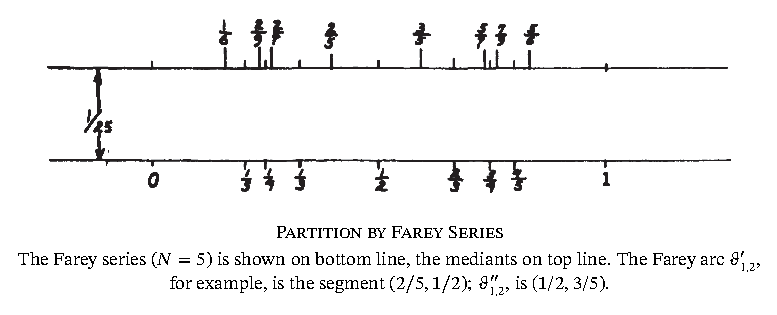
\includegraphics{chap01-vend-scan-08.eps}
\end{figure}

\begin{equation}
\label{ch01:eqn40} p(m)=\,\sum\limits_{k\leqq \sqrt{m}} k^{-1}A_{k}(m)f_{k}(m)\,+O(m^{-1/4}),
\end{equation}
where $f_{k}(m)$ is a certain entire function of $m$ asymptotic to $\exp C \sqrt{m}/k$ and $A_{k}(m)$ is a finite exponential sum involving the multipliers of $F$. The error term actually tends to $0$, a most surprising occurrence in analytic number theory, and so makes possible the \emph{calculation} of $p(m)$ for all sufficiently large $m$ as the nearest integer to the finite sum.\index{sum of squares}

The new method was soon applied to other problems of additive number theory, problems in which the generating function is not necessarily a modular form but does have a sharp asymptotic behavior. It became known as the Hardy-Littlewood\index{Hardy-Littlewood}\index{Littlewood} method and, in many variants, survives as a fundamental analytic tool in number theory.

Hardy and Ramanujan\index{Ramanujan} coupled the parameters $N$ and $m$. Rademacher\index{Rademacher}\index{Rademacher's partition series} left them independent and obtained instead of \eqref{ch01:eqn40}.
\begin{equation}
\label{ch01:eqn41} p(m)=\sum\limits_{k=1}^{N}k^{-1}A_{k}(m)g_{k}(m)+O(N^{-1/2}e^{2 \pi mN^{-2}}),
\end{equation}
where $g_{k}$, essentially a Bessel function, is slightly different from $f_{k}$ but has the same asymptotic value. \emph{If now} $m$ \emph{is held fixed while} $N\rightarrow\infty$, the error term tends to 0 and $p(m)$ is represented exactly by the \emph{convergent series} obtained by extending the finite sum to $\infty!$ \citeauthor{Rademacher0000}~[\ref{Rademacher1}]\index{Rademacher-Zuckerman} made this discovery in 1936 and he and \citeauthor{Zuckerman0000}~[\ref{Zuckerman1}]\index{Zuckerman} soon made use of it for the discussion of modular forms of arbitrary positive dimension. Then Zuckerman treated modular forms on subgroups of the modular group [\ref{Zuckerman2}] as well as forms with poles at interior points of $\mathscr{H}$, cf. [\ref{Zuckerman1}].

\begin{figure}[h]
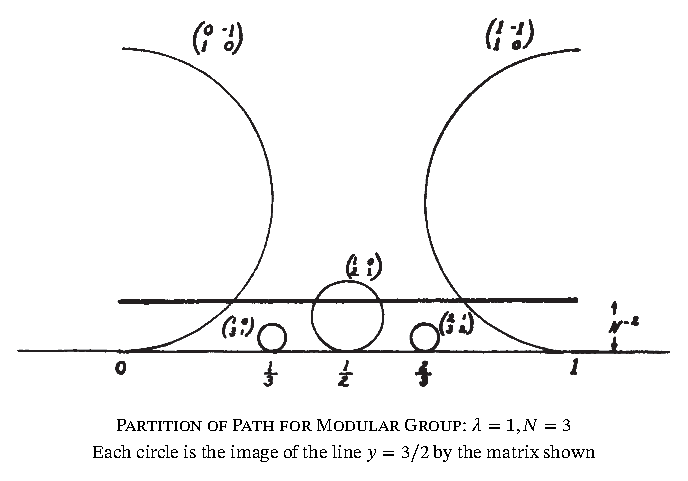
\includegraphics{chap01-vend-scan-09.eps}
\end{figure}

Recently the circle method has been applied to the classes $\{\Gamma, -r, v\}$, where $\Gamma$ is a group acting on $\mathscr{H}$ and possessing translations, the dimension $-r$ is positive, and $v$ is an arbitrary multiplier system (\citeauthor{Lehner0000}~[\ref{Lehner2}\index{Lehner, J.};~\ref{Lehner3};~\ref{Lehner4}]. The difficulty we face here is that the matrices are not known arithmetically and we cannot construct a Farey series. But we can construct a substitute for the Farey series as follows. The images of the horizontal line $y=h>0$ by all the elements of $\Gamma$ form a collection of circles tangent to the real axis, and these circles do not intersect if $h$ is large enough. We partition a line segment at height $N^{-2}$ above the real axis and of length $\lambda$, the, smallest translation of $\Gamma$, by intersecting it with the above system of circles (cf. Figure). The intervals lying within the circles are the important ones, those lying between the circles yield a negligible contribution. It is possible to derive enough information, essentially from the discreteness of $\Gamma$, to enable us to make all the required estimates, and we obtain as before convergent series representations of the expansion coefficients of the automorphic form. Forms with poles in the interior of $\mathscr{H}$ can also be handled.

Actually the matter is not quite so simple since in general there will be finite parabolic vertices $p_{1},\,\cdots,\,p_{s}$. There is an expansion for $F$ about each $p_{i}$. It is necessary to consider not $\Gamma$ but the systems $A_{j}\Gamma A_{k}^{-1},j=1,\cdots,s$, where $A_{j}$ sends $p_{j}$ to $\infty$, if we wish the expansion about $p_{k}$.

The circle method can also be used, in a modified manner, for forms of \emph{negative} dimension. \citeauthor{Hardy0000}~[\ref{Hardy1}]\index{Hardy|)}, following work of \citeauthor{Mordell0000}~[\ref{Mordell1}]\index{Mordell}, found for the number of representations $r_{s}(m)$ of $m$ by $s$ squares the formula
\begin{equation}
\label{ch01:eqn42} r_{s}(m)=\frac{\pi^{s/2}}{\Gamma(s/2)}m^{s/2-1} \mathfrak{S}(m)+O(m^{s/4}),\qquad
s\geqq 3
\end{equation}
where $\mathfrak{S}$ is the so-called ``singular series'' (\citeauthor{Dickson0000}~[\ref{Dickson1}\index{Dickson}, Ch. 13]). Here the generating function is
\begin{equation*}
\Theta(\tau)=(\vartheta_{3} (0|\tau))^{s} =\bigg(\sum\limits_{n=-\infty}^{\infty}e(n^{2}\tau /2)\bigg)^{s}=1+\sum\limits_{1}^{\infty}r_{s}(m) e(m_{\tau}/2),
\end{equation*}
with $\vartheta_{3}$ defined in \ref{ch01:sec1H}; $\Theta$ belongs to the class $\{\Gamma,\,-s/2, v\}$, where $\Gamma$ is the subgroup of the modular group generated by $\tau \rightarrow\tau +2, \tau\rightarrow -1/\tau$. By difficult considerations pertaining to the uniqueness of modular forms Hardy was able to show that the error term in \eqref{ch01:eqn42} is actually zero for $s=5,6,7,8$, and \citeauthor{Bateman0000a}~[\ref{Bateman1}]\index{Bateman, P. T.} completed the discussion for $s=3,4$. Thus $r_{s}(m)$ is given exactly by the first term of the right member.

This theory has been extended to the representations of integers by quadratic forms. Cf., for example, \citeauthor{Kloosterman0000}~[\ref{Kloosterman1}]\index{Kloosterman}, \citeauthor{Walfisz0000}~[\ref{Walfisz1}]\index{Walfisz}, and \citeauthor{Eichler0000}~[\ref{Eichler1}]\index{Eichler}.


\subsection{}\label{ch01:sec4B}\footnote{Cf. Ch.~\ref{ch08:chap08}.}
The original Poincar\'{e} series\index{Poincar\'{e} series} were automorphic forms of \emph{negative} integral dimension $\leqq-3$. When we try to define them for groups acting on the upper half-plane $\mathscr{H}$, we encounter a new difficulty. Consider
\begin{equation*}\tag{$^{\ast}$}
 \sum\limits_{V \in \Gamma}\,(c\tau +d)^{-k},\quad k= \mathrm{integer},\qquad V=\left(\begin{matrix}
a & b\\ c & d
\end{matrix}\right)
\end{equation*}
where $\Gamma$ possesses translations generated by $S\tau=\tau +\lambda$. Every element fixing $\infty$ is a translation and we may therefore write $\{S^{m},\,m=\mathrm{integer})=\Gamma_{\infty}$. Since $S^{m}V\in\Gamma$ and also has $(c, d)$ as its lower row, the term $(c\tau+d)^{-k}$ occurs infinitely often and the series $(^{\ast})$ cannot converge. Hecke\index{Hecke} got around the difficulty by summing over a set of representatives of the cosets $\Gamma_{\infty}\backslash \Gamma$, i.e., a complete system of matrices of $\Gamma$ with different lower row. He called the series
\begin{equation}\label{ch01:eqn43}
 E(\tau)=\sum\limits_{V \in \Gamma_{\infty}\backslash \Gamma}(c\tau+d)^{-k},\qquad k= \mathrm{integer}\ \geqq 3
\end{equation}
an \emph{Eisenstein} series. It belongs to the class $\{\Gamma, -k, 1\}$ and is regular in $\mathscr{H}$ and at the parabolic cusps of $\Gamma$. (Cf. [\citeauthor{Hecke0000}~\ref{Hecke1}, pp. 461--486]).

Hecke studied these series for $\Gamma$ a congruence subgroup of level $N$. Let $\mathscr{H}^{+}$ be $\mathscr{H}$ together with the parabolic cusps of $\Gamma$. He defined a set of Eisenstein series\index{Eisenstein series} $\{E_{j}\}$, one for each inequivalent cusp $p_{j}$, such that $E_{j}$ has the value 1 at $p_{j}$ and 0
at the other cusps. If $F\in\{\Gamma, -k, 1\}$ and is regular in $\mathscr{H}^{+}$, then $F$ minus a suitable linear combination of the $\{E_{j}\}$ vanishes at all parabolic cusps, i.e., is a \emph{cusp form}\index{covering transformation}. This decomposition\index{Decomposition theorem for automorphic forms},
\begin{equation*}\tag{$\dagger$}
 F(\tau)=\sum b_{j}E_{j}(\tau)+C(\tau),
\end{equation*}
$C$ being a cusp form, is unique.

Suppose now $F$ has the Fourier\index{modular form!Fourier coefficients of} series $F(\tau)=\sum\nolimits_{0}^{\infty}a_{m}e(m\tau/N)$. Then $a_{m}=\sum\nolimits_{1}^{h}b_{j}e_{m}^{(j)}+c_{m}$, in an obvious notation. The $e_{m}^{(j)}$ can be calculated explicitly, while the $c_{m}$ carry the estimate
\begin{equation}\label{ch01:eqn44}
 c_{m}=O(m^{k/2}),
\end{equation}
as Hecke himself showed by a very simple proof. Then we have
\begin{equation}\label{ch01:eqn45}
a_{m}=\sum\limits_{j=1}^{h}b_{j}e_{m}^{(j)}+O(m^{k/2}).
\end{equation}
For example, if $F=(\vartheta_{3}(0|\tau))^{s}$ with $s$ an even integer, this equation becomes \eqref{ch01:eqn42} for the number of representations of $m$ by $s$ squares.

The cusp forms constitute a vector space $\mathbf{C}^{0}$ of known finite dimension. If $\mathbf{C}^{0}$ contains only 0, we can drop the error term in \eqref{ch01:eqn45} and have an exact formula. If a basis for $\mathbf{C}^{0}$ is known, we can determine the coefficients of the cusp forms entering into $(\dagger)$ by utilizing a finite number of coefficients in the Fourier expansions of the functions involved. This method is theoretically applicable for all values of $s$ whereas the singular series is known to give an incorrect result for $s>8$.

Hecke's investigations of modular forms may be regarded as an elaboration and deepening of the Klein-Fricke\index{Fricke}\index{Fricke-Klein}\index{Klein, F.} program.\footnote{Cf. \citeauthor{Fricke0000a} [\ref{Fricke3a}]; [\ref{Fricke4}].} He studied the algebraic function field $K$ defined by a principal congruence subgroup, the group of automorphisms of $K$, the integrals on $K$, their periods, etc. Almost always he was motivated by a number-theoretic problem and his results contain some of the finest achievements of analytic number theory.

Perhaps Hecke's\index{Hecke} most significant result is his beautiful theory of Dirichlet series with Euler products, which involves the vector space of regular modular forms of a given dimension and has applications in the arithmetic theory of quadratic forms. For a brief account cf. \citeauthor{Hecke0000} [\ref{Hecke1}, pp. 577--590].


\subsection{}\label{ch01:sec4C}\footnote{Cf. Ch.~\ref{ch08:chap08}.}
The most important contributor to the theory of automorphic functions in recent times is H. Petersson\index{Petersson|(}, whose investigations begin about 1930. He was a student of Hecke and much of his work consists in extending to more general discontinuous groups what Hecke developed for congruence subgroups of the modular group. Petersson, like Klein\index{Klein, F.} and Hecke, is greatly interested in the correspondence between Riemann surface theory and automorphic\index{scalar product of automorphic forms} function theory. Because he insists on considerable generality, his papers are hard to read, but it is also true that he returns again and again to the classical examples from which the general theory sprang, reinterpreting and deepening them with the newer results.

Petersson works with groups $\Gamma$ defined on the upper half-plane $\mathscr{H}$, which he regards as the uniformizing plane of a compact Riemann surface. Thus $\Gamma$ has a fundamental region with a finite number of sides and it admits only finitely many classes of elliptic and parabolic transformations.

In [\ref{Petersson1}] Petersson defined a new type of Poincar\'{e} series\index{Poincar\'{e} series}, more general than the Eisenstein series\index{Eisenstein series}. Let the class $\{\Gamma, -r, v\}$ be given, with $v$ a multiplier system\index{multiplier system} and $r>2$. Let
\begin{equation}\label{ch01:eqn46}
G_{-r}(\tau, v, \nu+\kappa_{0}) =\sum\limits_{T\in\Gamma_{\infty}\backslash \Gamma}\frac{e((\nu+\kappa_{0}) T/\lambda_{0})}{v(T)(c\tau+d)^{r}},\qquad T=\left(\begin{matrix} \cdot & \cdot \\
c & d\end{matrix}\right).
\end{equation}
Here $e(u)=\exp 2\pi iu,\,\nu$ is an integer, $S\tau =\tau+\lambda_{0}$ generates the subgroup $\Gamma_{\infty}$, and $\kappa_{0}$ is defined by $v(S)=e(\kappa_{0}), 0\leqq \kappa_{0}< 1$. To take care of the many-valuedness of $(c\tau +d)^{r}$ we shall demand that the multiplier system $v$ satisfy a consistency condition: for $T_{1},\, T_{2}\in\Gamma$
\begin{align}\label{ch01:eqn47} v(T_{1}T_{2})(c_{12}\tau+d_{12})^{r}=v(T_{1})(c_{1}T_{2}\tau+d_{2})^{r}&v(T_{2})(c_{2}\tau+d_{2})^{r},\\
&\ T_{1}T_{2}=\left(\begin{matrix} \cdot & \cdot \\
c_{12} & d_{12}\end{matrix}\right)\nonumber
\end{align}
which reduces to $v(T_{1}T_{2})=v(T_{1}) v(T_{2})$ when $r$ is an integer. Petersson proved the existence of multiplier systems $v$ of absolute value 1 satisfying \eqref{ch01:eqn47}. Poincar\'{e}'s\index{Poincar\'{e}} noneuclidean convergence proof applies to \eqref{ch01:eqn46}, after which we can easily show that $G_{-r}\in\{\Gamma, -r, v\}$. This is the series appropriate to the cusp $\infty$; there is an analogous series $G_{-r}(\tau, v, A_{j},\nu+K_{j})$, which behaves at $p_{j}=A_{j}^{-1}\infty$ as the original series does at $\infty$.

In particular, if $\nu+\kappa_{j} < 0$, the series $G_{-r}(\tau, A_{j})$ has a pole at $p_{j}$ and cannot vanish identically. If $\nu+\kappa_{j} >0$, the series vanishes at all parabolic cusps and so is a cusp form (which may of course be identically zero). If $\nu=\kappa_{j}=0,\,G$ is an Eisenstein series: it has the value 2 at $p_{j}$ and 0 at the other cusps.

In 1939 Petersson introduced the very important scalar product\footnote{A similar scalar product is used in the theory of differentials on Riemann surfaces (\citeauthor{Springer0000}~[\ref{Springer1}],\index{Springer} Ch. 7).} of automorphic forms ([\ref{Petersson2}; \ref{Petersson3}]). For $f,\,g\in\{\Gamma, -r, v\}$ and regular in $\mathscr{H}^{+}$ we define
\begin{equation}\label{ch01:eqn48}
(f, g)=\int\int\limits_{R} f(\tau)\overline{g(\tau)}y^{r-2}dx\,dy,\qquad r>2,
\end{equation}
where $R$ is a fundamental region of $\Gamma$. The integral converges if either $f$ or $g$ is a cusp form. Thus the subset of $\{\Gamma, -r, v\}$ consisting of all cusp forms becomes a Hilbert space\index{Hilbert space of automorphic forms} $\mathbf{C}^{0}$ under the scalar product \eqref{ch01:eqn48}. It is easy to show $\mathbf{C}^{0}$ is of finite dimension. Furthermore, we can discuss the orthogonality of a form in $\mathbf{C}^{0}$ with a form in $\mathbf{C}^{+}$, the vector space of elements of $\{\Gamma, -r, v\}$ that are regular in $\mathscr{H}^{+}\ (=\mathscr{H}+$ parabolic cusps), we can construct orthogonal complements, etc. The dimension of $\mathbf{C}^{+}$ can be calculated from the Riemann-Roch theorem (\ref{ch06:chap06}. \ref{ch06:sec4}).

Petersson's investigations of the new Hilbert spaces revolutionized the theory of automorphic forms of negative dimension. Formerly difficult theorems could now be proved by the methods of linear algebra. Here are some results. The Poincar\'{e} series $\{G_{-r}(\tau, v,\, \nu+\kappa_{0}),\ \nu=0,1,\cdots,
\nu+\kappa_{0} >0\}$ span the space $\mathbf{C}^{0}$ of cusp forms. The orthogonal complement of $\mathbf{C}^{0}$ in $\mathbf{C}^{+}$ is the space of Eisenstein series (generalization of the Hecke Decomposition Theorem). The linear relations among the Poincar\'{e} series (which must exist because there are infinitely many Poincar\'{e} series and $\dim\ \mathbf{C}^{0}$ is finite) are expressible as linear relations among their Fourier coefficients, and conversely. A Poincar\'{e} series with parameter $\nu$ vanishes identically if and only if its $\nu$th Fourier coefficient is zero; it is characterized (up to a multiplicative constant) as that cusp form which is orthogonal to the linear manifold of cusp forms having zero $\nu$th Fourier coefficients. The first $\mu$ Poincar\'{e} series $G_{-r}(\tau,1,1), \cdots,\,G_{-r}(\tau, 1,\,\mu)$ form a basis for the space of cusp forms of the modular group with multipliers identically 1, where $\mu$ is the dimension of the space.

We have so far assumed $r>2$. Practically nothing is known about the range $0<r<2$. The forms of dimension $-2,\,v\equiv 1$, are important because they correspond to the \emph{abelian differentials}\index{abelian differentials} on Riemann surfaces (\ref{ch06:chap06}. \ref{ch06:sec4}):
\begin{equation*}
F(V\tau) d\, V\,\tau=F(\tau) d\tau,\qquad V\in\Gamma.
\end{equation*}
The Poincar\'{e} series of dimension $-2$ does not converge absolutely. Hecke\index{Hecke} ([\ref{Hecke1}, pp. 468-476]) inserted a convergence factor\index{Hecke's convergence factor}:
\begin{equation}\label{ch01:eqn49}
E_{2}(\tau)=\lim\limits_{n\rightarrow 0} E_{2}(\tau, s);\qquad E_{2}(\tau,s)=\sum\limits_{m,n} (m\tau + n)^{-2}|m\tau+n|^{-s}
\end{equation}
where $s$ is a variable. Clearly $E_{2}(\tau, s)$ has the transformation Property of a form of dimension $-2$ and Hecke showed that the limit exists. Thus $E_{2}(\tau)$ is a modular form. Petersson exploited the method for general Poincar\'{e} series in the class $\{\Gamma(n), -2,1\}$, introducing a scalar product and carrying over the previous results for $r>2$ (\citeauthor{Petersson0000}~[\ref{Petersson9}]). Later he generalized to a larger class of groups and multipliers ([\ref{Petersson10}]).

For $r\geqq 2$ the everywhere regular automorphic forms can be represented as finite linear combinations of Poincar\'{e} series (with certain restrictions when $r =2)$, which can then be expanded in Fourier series. Hence the Fourier coefficients of everywhere regular forms are given by explicit series expansions; these are of the same structure as Rademacher's\index{Rademacher} partition series.

As an example consider $J^{\prime}(\tau)$\index{$j(\tau)$}, the derivative of the Dedekind-Klein modular invariant \eqref{ch01:eqn10}. $J^{\prime}$ is in the class $\{\Gamma(1), -2,1\}$ and has a simple pole at $\infty$ and is otherwise regular. Now there are no nonzero cusp forms in this class. Hence $J^{\prime}$ is a constant multiple of the Poincar\'{e} series $G_{-2}(\tau, 1, \nu+\kappa_{0})$ with $\kappa_{0}=0,\,\nu=-1$. Since the coefficients of $G_{-2}$ are known explicitly, we obtain by integration the coefficients of $J$:
\begin{equation}\label{ch01:eqn50}
\begin{split}
12^{3}J(\tau)&=e(-\tau)\,+c_{0}+\sum\limits_{n=1}^{\infty}c_{n}e(n\tau),\\
c_{n}=2\pi n^{-1/2}\ &\sum\limits_{k=1}^{\infty}k^{-1}A_{k}(n)I_{1}(4\pi n^{1/2}/k),\qquad n\geqq 1,
\end{split}
\end{equation}
$I_{1}$ being the Bessel function and
\begin{equation}
\label{ch01:eqn51} A_{k}(n)=\,\sum\limits_{\substack{h=0 \\ (h,k)=1}}^{k-1} e(-(nh+h^{\prime})/k),\qquad hh^{\prime}\equiv-1\ (\mathrm{mod}\,k).
\end{equation}
This beautiful and important result appears with no special emphasis in the middle of a long paper (\citeauthor{Petersson0000}~[\ref{Petersson9}, p. 202]).

In general, however, the integral of an abelian differential\index{abelian differentials} (automorphic form of dimension $-2$ with $v\equiv 1)$ is not an automorphic function; it is an \emph{abelian integral}, a meromorphic function $F$ satisfying
\begin{equation*}
F(L\tau)=F(\tau)+C(L),\qquad L\in \Gamma,
\end{equation*}
where the ``period'' $C(L)$ is independent of $\tau$. Recently \citeauthor{Petersson0000}~[\ref{Petersson11}] has carried over his theory of the scalar product to the study of abelian integrals.

As a result of Petersson's lengthy investigations there is now a rather complete theory analogizing the classical theory of functions and differentials on compact Riemann surfaces.

~\citeauthor{Bers0000}~[\ref{Bers1}]\index{Bers} has now generalized some of Petersson's results to \emph{infinitely generated} groups\index{infinitely generated groups}. For $\Gamma$ a group of linear transformations of the unit disk $\mathscr{U}$, he proves, for dimensions $<-2$, that the space of Poincar\'{e} series \eqref{ch01:eqn33} \emph{with} $H(z)$ \emph{a polynomial} is dense in the space of all autuomorphic forms regular in $\mathscr{U}$ and satisfying a certain growth condition.


\subsection{}\label{ch01:sec4D}
Petersson also treated forms of positive dimension ([\ref{Petersson6}; \ref{Petersson7}]; \ref{Petersson8}]). Such a form most have poles if it is not to be a constant (\ref{ch09:chap09}. 2M) and so is determined uniquely by its principal parts\index{principal parts}. But the principal parts cannot be assigned arbitrarily. For suppose $F\in\{\Gamma,\,-r,\, v)$; let $G$ belong to the \emph{complementary class} $\{\Gamma,\,r-2,\, v^{-1})$. Then $FG\in\{\Gamma, -2, 1\}$, i.e., it is an abelian differential. Hence the sum of the residues of $FG$ vanishes, and this gives a requirement the principal parts of $F$ must satisfy. If there are $\mu$ independent cusp forms $G_{j}$, there are $\mu$ conditions which, collectively, are known as the \emph{principal-parts condition}. This condition is therefore necessary for the existence of a form $F$ with preassigned principal parts; Petersson showed it to be sufficient.

For the construction forms in the class $\{\Gamma, r -2, v^{-1}\}$ --- thus of positive dimension---Petersson used a classical principle, ``interchange of argument and parameter,''\index{interchange of argument and parameter} already mentioned in \citeauthor{Ritter0000}~[\ref{Ritter1}].\index{Ritter} Consider for $r>2,\,\kappa_{0} >0$,
\begin{align}\label{ch01:eqn52}
H(\tau, z)=e((1-\kappa_{0})z) \sum\limits_{M\in \Gamma_{\infty}\backslash \Gamma}\frac{e(\kappa_{0}\tau)}{e(M\tau)-e(z)}\cdot&\frac{1}{v(M)(c\tau+d)^{r}},\\
&\qquad M=\,\left( \begin{matrix} \cdot & \cdot\\ c & d \end{matrix}\right).\nonumber
\end{align}
As a function of $\tau,\,H$ is in the class $\{\Gamma, -r, v\}$ and is regular in $\mathscr{H}^{+}$ with the exception of a simple pole at $z$ and equivalent points. As a function of $z$, however, $H$ has the transformation formula
\begin{align}\label{ch01:eqn53}
 H (\tau, Lz)=v^{-1}(L)(\gamma z+\delta)^{2-r} H(\tau, z)+\ &\Omega (\tau, z,\, L),\\
&\quad L=\,\left(\begin{matrix} \cdot & \cdot \\ \gamma & \delta\end{matrix}\right)\in\Gamma \nonumber
\end{align}
that is, except for the additive term $\Omega,\,H$ has the behavior of a form in $\{\Gamma, r-2, v^{-1}\}$. A suitable linear combination $F$ of functions of the type of $H$ satisfies \eqref{ch01:eqn53} with $\Omega$ replaced by 0; $F$, then, is in $\{\Gamma, r-2, v^{-1}\}$. For this it is necessary and sufficient that the principal parts of $F$ satisfy the principal-parts condition. Hence all automorphic forms of positive dimension\index{automorphic forms of positive dimension} can be expressed as linear combinations $F$, and conversely, every such linear combination satisfying the principal-parts condition is an automorphic form. The functions $H$ can be expanded in Fourier series, and so we obtain the same infinite series representations of the expansion coefficients of the form that are got from the circle method\footnote{Petersson's work on this problem was done in 1950-54, after Rademacher-Zuckerman\index{Zuckerman} but before Lehner\index{Lehner, J.}.}  (\ref{ch01:sec4A}).


\subsection{}\label{ch01:sec4E}
We have seen\index{Hecke's convergence factor}\index{Poincar\'{e} series!conditional convergence of} (\ref{ch01:sec4C}) how the Fourier coefficients of automorphic functions can be obtained by integrating forms of dimension $-2$. They can also be obtained by the circle method. Applied to a form of nonnegative dimension\footnote{Unfortunately the notations of Petersson and Rademacher disagree; the latter denotes the dimension of a form by $r$. We are following Petersson in this respect.}  $-r\ (r\leqq 0)$, the circle method produces an error term $O(N^{-r})$, which for a function $(r=0)$ means only a hounded error. The formal series obtained by the circle method does converge, but it is in no way obvious that it converges to the function. Rademacher showed how to overcome the difficulty in the case of the modular invariant $J(\tau)$\index{$j(\tau)$}.

The trick is to obtain and utilize a better estimate of the exponential sums $A_{k}(n)$ (cf. \eqref{ch01:eqn51}). A trivial estimate is $O(k)$. But such sums had arisen in the application of the circle method to representations of integers by quadratic forms, and in connection with such problems \citeauthor{Kloosterman0000}~[\ref{Kloosterman1}]\index{Kloosterman} was led to study the sums $S_{k}(n)$ now named after him:
\begin{equation*}
S_{k}(n)=\,\sum\limits_{\substack{h=0\\ (h,k)=1}}^{k-1} e(nh+h^{\prime}),\qquad hh^{\prime}\equiv-1\,(\mathrm{mod}\, k).
\end{equation*}
He showed that
\begin{equation}
\label{ch01:eqn54} S_{k}(n)=O(k^{1-\alpha+s} (n,k)^{n})
\end{equation}
for a certain positive $\alpha$, not only for this sum but for others in which additional restrictions are imposed on $h$.

By making use of the improved estimate and handling the summations more carefully, \citeauthor{Rademacher0000}~[\ref{Rademacher3}]\index{Rademacher} reduced the error term in the circle method from $O(1)$ to $O(N^{-\alpha+\epsilon})$ and so proved that the formal series for $J(\tau)$ actually represents it. The method was applied by his students in special cases to functions of class $\{\Gamma, 0, v\}$, where $\Gamma$ is a congruence subgroup and $v\not\equiv 1$. Then the sum $A_{k}(n)$ is more complicated since it involves the multipliers, but must in each case be reduced to a Kloosterman sum\index{Kloosterman sum}. The method will doubtless be successful whenever $v$ is a \emph{congruence character}, which means that $v\equiv 1$ on some $\Gamma(n)\subset\Gamma$, for in this case \citeauthor{Petersson0000}~[\ref{Petersson10}]\index{Petersson|)} has shown the reduction to Kloosterman sums is always possible.

The Kloosterman sums themselves were the subject of a series of papers involving, among others, the names of Estermann\index{Estermann}, Sali\'{e},\index{Sali\'{e}} and Davenport\index{Davenport}, until in 1948 \citeauthor{Weil0000}~[\ref{Weil1}]\index{Weil, A.} proved the long standing conjecture
\begin{equation}
\label{ch01:eqn55} |S_{p}(n)|\leqq 2 \sqrt{p},\qquad p=\mathrm{prime},\ (p,\,n)=1.
\end{equation}
With previous results this leads to
\begin{equation}\label{ch01:eqn56}
S_{k}(n) =O(k^{1/2+\epsilon}(n, k)^{1/2}).
\end{equation}
It is curious\index{Lehner, J.} that \eqref{ch01:eqn56} could be proved in an elementary way by Sali\'{e}\index{Sali\'{e}} for each $k$ that contains at least the square of every prime dividing it. Weil's\index{Weil, A.} proof is assuredly difficult as well as recondite; it depends completely on his theorem asserting the truth of Riemann Hypothesis in an algebraic function field over a finite field, about which he had written a book the year before. So far \eqref{ch01:eqn55} has resisted all attempts at an elementary proof.


\subsection{}\label{ch01:sec4F}
We now turn to a converse problem. Given a class $\{\Gamma, -r, v\}$ with associated parameters $\kappa_{0},\lambda_{0}$, how can we choose constants $a_{m}$ so that the function
\begin{equation}\label{ch01:eqn57}
F(\tau)=\sum a_{m}e((m +\kappa_{0}) \tau/\lambda_{0})
\end{equation}
is an antomorhic form belonging to this class? The solution to this problem will be of importance in all those cases in which there is no easy method (such as the Poincar\'{e} series) for generating automorphic forms. Thus we shall be most interested in $r\leqq 2$.

Let us, however, first consider $r>2$. Here we naturally choose for $a_{m}$ the known infinite series expression got by expanding the Poincar\'{e} series in a Fourier series (cf. \ref{ch01:sec4C}). We insert this in \eqref{ch01:eqn57} and rearrange the resulting double series in a series of partial fractions, in other words, the original Poincar\'{e} series. In this way we see that $F$ has the desired transformation properties. All these manipulations are easy because the series involved converge absolutely. In fact this is the route followed by Hardy\index{Hardy} in his investigation of the representation problem by squares (cf. end of \ref{ch01:sec4A}). But for dimension $\geqq-2$ absolute convergence, or even convergence, fails.

By means of Hecke's\index{Hecke} convergence factor one can handle the case $-r=-2$ provided $\Gamma$ is restricted to a class of congruence subgroups and $v$ is also restricted (cf. \eqref{ch01:eqn49}). This case can also be treated by summing the Poincar\'{e} series in a certain order to obtain conditional convergence; the validity of rearrangement then has to be shown directly (\citeauthor{Lehner0000}~[\ref{Lehner6}]; J. R. \citeauthor{Smart0000}~[\ref{Smart1}]).\index{Smart, J. R.}

The latter method is based on a technique invented by \citeauthor{Rademacher0000}~[\ref{Rademacher4}]\index{Rademacher}. He considered our problem for the function $J(\tau)$. If $c_{n}$ is given by \eqref{ch01:eqn50}, then, as Rademacher\index{$J(\tau)$!Rademacher's partial fraction series for} proved,
\begin{equation}\label{ch01:eqn58}
\begin{split}
& e(-\tau)+\sum\limits_{n=1}^{\gamma}c_{n}e(n\tau)=e(-\tau)+e(1/\tau)-\,13\\
+\ & \lim\limits_{K\rightarrow \infty}\sum\limits_{k=1}^{K}\sum\limits_{\substack{1\leqq|m|\leqq K \\ (m,k)=1}} \bigg \{ e\Big( \frac{-m^{\prime}\tau - k^{\prime}}{k \tau- m}\Big) - e \Big( - \frac{m^{\prime}}{k}\Big) \bigg\},
\end{split}
\end{equation}
where
\begin{equation*}
mm^{\prime}+kk^{\prime}-1=\,0.
\end{equation*}
The left member is obviously invariant under $\tau \rightarrow \tau+1$ and it is not hard to show that the right member is invariant under $\tau \rightarrow-1/\tau$. The function defined by \eqref{ch01:eqn58} is therefore a modular function regular in $\mathscr{H}$ and having a simple pole at $\infty$ with residue 1. It must therefore coincide will $J$ up to an additive constant. Thus we obtain an expansion of $J$ into partial fractions\index{$J(\tau)$!Rademacher's partial fraction series for} which may be compared with that of the Weierstrass\index{Weierstrass} function $\wp$ (cf. \eqref{ch01:eqn1}); note the subtracted ``convergence summand'' in each case. The formula \eqref{ch01:eqn58} is as striking and  elegant as the classic identities of Euler\index{Euler} and Jacobi\index{Jacobi}.

Similar formulas can doubtless be obtained for restricted classes of congruence subgroups and multipliers. There seems to be no hope at the present time of extending these results to more general discontinuous groups.

Let us now consider the same problem for forms of \emph{positive} dimension. We shall describe some recent work of M. I. Knopp\index{Knopp, M. I.}. Let $-r$ be a positive \emph{integer}. Let
\begin{equation}\label{ch01:eqn59}
e(-\kappa_{0}\tau/\lambda_{0})F_{\mu}(\tau)= e(-\mu \tau/\lambda_{0})+ \sum\limits_{m=0}^{\infty} a_{m}e(m \tau / \lambda_{0}).
\end{equation}
Here
\begin{equation*}\tag{$^{\ast}$}
 a_{m}=a_{m}(\mu, -r,\, v)
\end{equation*}
is the infinite series given (for example) by the circle method in the case of a form in $\{\Gamma, -r, v\}$ with the same principal part as $F_{\mu}$. We do not assume such a form exists; the circle method yields an expression for $a_{m}$ in any case. The function $F_{\mu}$ is regarded as being \emph{defined} by \eqref{ch01:eqn59}.

In general $F_{\mu}$ will not be an automorphic form, but \citeauthor{Knopp0000}~[\ref{Knopp1}] showed there is a transformation formula\index{Knopp's transformation formula}
\begin{equation}
\label{ch01:eqn60} F_{\mu}(M\tau)=v(M)(c\tau+d)^{r}F_{\mu}(\tau) - v(M)(c\tau+d)^{r}p_{M}(\tau,\,\mu,\, v),\qquad M\in\Gamma.
\end{equation}
where $p_{M}$ is a \emph{polynomial} in $\tau$ of degree at most $-r$. This reminds us of Petersson's\index{Petersson} result \eqref{ch01:eqn53}. By a suitable linear combination $F$ of a set of $F_{\mu}$ with different $\mu$ we can make the polynomial $p_{M}$ disappear. Then $F$ will be a form in $\{\Gamma, -r, v\}$. Thus our original goal, the construction of forms of positive dimension, has been achieved, at least for integral dimensions. It is most desirable that Knopp's theorem should be extended to non-integral $r$.

Conversely, if $F$ is given as a form of $\{\Gamma, -r, v\}$ with given principal part, we obtain its Fourier coefficients by the circle method.

The problem of deciding whether $F_{\mu}$ is actually a form is solved by the introduction of the \emph{supplementary series}\index{supplementary series}
\begin{equation*}
e(-\kappa_{0}^{\prime}\tau/\lambda_{0}) \bar{F}_{\mu^{\prime}} (\tau)=e(-\mu^{\prime}\tau)+\sum\limits_{m=0}^{\infty} \hat{a}_{m}e(m\tau/\lambda_{0})
\end{equation*}
where $(\kappa_{0}>0)$
\begin{equation*}
\hat{a}_{m}=a_{m}(\mu^{\prime},\,-r,\, v^{-1}),\qquad \mu^{\prime}=1-\mu,\qquad  \kappa_{0}^{\prime}=1-\kappa_{0}
\end{equation*}
in the notation $(^{\ast})$. There $F_{\mu}\in\{\Gamma, -r, v\}$ if and only if $\hat{F}_{\mu^{\prime}}\equiv 0$. Then is a similar criterion involving Poincar\'{e} series $G_{-r^{\prime}}(\tau, v^{-1}, \mu-\kappa_{0}),r^{\prime}=2-r$, belonging to the complementary class $\{\Gamma, -r^{\prime}, v^{-1}\}$, namely, $F_{\mu}\in\{\Gamma, -r, v\}$ if and only if $G_{-r^{\prime}}\equiv 0$. (Cf. \citeauthor{Knopp0000a}\index{Knopp, M. I.}\index{Lehner, J.} [\ref{Knopp}]; also \ref{ch09:chap09}. \ref{ch09:sec3F}.)

Knopp has also applied his method to the construction of modular functions and abelian integrals ([\ref{Knopp2}; \ref{Knopp3}; \ref{Knopp4}]).

The circle method and the method of Poincar\'{e} series seem to be two sides of the same coin. In the next few years we may expect further elucidation of this connection.


\subsection{}\label{ch01:sec4G} \footnote{Cf. Ch.~\ref{ch10:chap10}.}
Let $\Gamma$ be a Fuchsian (finitely generated) group acting on the unit disk $\mathscr{U}$. If we identify points of $\mathscr{U}$ that are equivalent under $\Gamma$, we obtain a two-dimensional Riemannian manifold $\mathbf{F}$ of constant negative curvature\index{manifold of constant negative curvature}, on which the metric is defined by  transplanting the Poincar\'{e} hyperbolic metric of $\mathscr{U}$ (cf. \ref{ch02:chap02}. \ref{ch02:sec12}). A geodesic on $\mathbf{F}$ is represented by a hyperbolic line on $\mathscr{U}$ together with all its images under $\Gamma$. In the twenties and thirties a number of mathematicians investigated problems concerning the behavior of geodesics and other curves on $\mathbf{F}$, which arose in the study of the possible motions of dynamical systems, by interpreting them as problems concerning hyperbolic lines, horocycles, etc., on $\mathscr{U}$.

Of particular interest is a phenomenon called transitivity\index{transitivity} (ergodicity). In $\mathscr{U}$ this may be described as follows. If $L$ is a hyperbolic line starting from a point of $\mathscr{U}$ and ending in a parabolic cusp of $\Gamma$, it crosses a finite number of fundamental regions and its image in a fixed fundamental region $R_{0}$ consists of a finite number of arcs. But if $L$ terminates in a point that is not a parabolic vertex, the image of $L$ consists of infinitely many arcs and it can happen that the image set is everywhere dense in $R_{0}$ (equivalently, the set $\Gamma L$ is dense in the set of all hyperbolic lines in $\mathscr{U}$). Then we say $L$ is a \emph{transitive} $H$-\emph{ray}.

The existence of transitive rays was proved for the modular group in 1924 by \citeauthor{Artin0000}~[\ref{Artin1}]\index{Artin} and P. J. \citeauthor{Myrberg0000}~[\ref{Myrberg1}]\index{Myrberg}, and \citeauthor{Koebe0000}~[\ref{Koebe1}]\index{Koebe} in 1930 gave a proof for all horocyclic \footnote{I.e., every point of the unit circle is a limit point of $\Gamma$.} groups. (It is obvious there can be no transitive rays if $\Gamma$ is not horocyclic.)

We are also interested in the \emph{measure} of the transitive $H$-rays, but it is simpler to consider the measure of their endpoints. A \emph{point} of $\mathscr{Q}$, the unit circle, is called \emph{transitive} if every $H$-ray through the point is transitive; otherwise the point is termed \emph{intransitive}. In 1931 \citeauthor{Myrberg0000}~[\ref{Myrberg2}] proved: \emph{The set of intransitive points is of Lebesgue measure zero}. This obviously implies that the values assumed by an automorphic function $f(z)$, as $z$ approaches a transitive point on a hyperbolic line, are dense in the set of complex numbers. Myrberg also showed that the intransitive points are uncountable. Both results were proved for a certain subclass of horocyclic groups.

A few years later E. \citeauthor{Hopf0000}~[\ref{Hopf1}]\index{Hopf, E.} gave a proof of the property known as  \emph{metric transitivity}\index{metric transitivity}, from which Myrberg's\index{Myrberg} first result follows (for all horocyclic groups). Consider the torus $\mathscr{R}=\mathscr{Q}\times\mathscr{Q}$. We shall say a subset $S$ of $\mathscr{R}$ is $\Gamma$-invariant if the set $\{(Vz_{1}, Vz_{2})\,|\,z_{1},\,z_{1}\in S\}$ equals $S$ for all $V\in\Gamma$. Then $\Gamma$ is said to be metrically transitive if each $\Gamma$-invariant set $S$ has 2-dimensional measure 0 or $4\pi^{2}$. In a proof combining harmonic function theory with the theory of Fuchsian groups, \citeauthor{Hopf0000}~[\ref{Hopf1}] proved that every horocyclic group is metrically transitive. Other proofs were given subsequently by \citeauthor{Hedlund0000}~[\ref{Hedlund3}]\index{Hedlund} and \citeauthor{Tsuji0000}~[\ref{Tsuji2}].\index{Tsuji, M.}

For a readable account of this subject, including the connection with dynamics, cf. \citeauthor{Hedlund0000}~[\ref{Hedlund2}].

We must also mention work on discontinuous groups considered as \emph{abstract} groups. There is, for example, the theorem of \citeauthor{Nielsen0000}~[\ref{Nielsen1}]\index{Nielsen, J.} (cf. also \citeauthor{Lauritzen0000}~[\ref{Lauritzen1}]\index{Lauritzen, S.}) that a nonabelian group consisting of $2\times2$ hyperbolic matrices with real elements is discontinuous in the upper half-plane. In the same paper Nielsen found a necessary and sufficient condition, of a geometric character, that such a group be finitely generated. The work of Nielsen, Schreier,\index{Schreier, O.} and Reidemeister\index{Reidemeister} on free groups created new interest in the group structure of the congruence subgroups of the modular group, which had not been studied since Klein\index{Klein, F.}. (The principal congruence subgroups of level greater than 1 are free groups.) Our knowledge on this point is still incomplete despite continuing active investigation.


\subsection{}\label{ch01:sec4H}
Almost as soon as the theory of automorphic functions was founded, mathematicians were aware of the possibility of extending it to functions of several complex variables. But interest was relatively low until 1939 when C. L. \citeauthor{Siegel0000}~[\ref{Siegel5}]\index{Siegel, C. L.} introduced matrix modular forms in connection with his theory of quadratic forms. Since then the subject has developed rapidly and the literature is now vast. A reasonably complete account would occupy a volume as large as this one. Such a book is urgently needed at the present time.

In Ch.~\ref{ch12:chap12} we present a sketch of the theory and prove some of the fundamental theorems.


\subsection{}\label{ch01:sec4I}
The preceding survey, of course, did not touch on all lines of investigation connected with our subject. The writer does not mean to imply that the omitted topics are less important or of less worth mathematically than those which were included. Considerations of space made a choice mandatory, and we have tried to select those developments which are most in keeping with the remainder of the book. Even so we have doubtless overemphasized, unintentionally, some contributions at the expense of others, but we hope to have imparted a reasonable view of our many-sided subject.


%%%%%%%%chapter02

\chapter{Preparatory Material}\label{ch02:chap02}

This chapter will not be read systematically by the mature mathematician. It has been written primarily with the needs of the student in mind. These pages are not intended to initiate him into the subjects discussed (except for certain special topics like the Isometric Circle); he is presumably already familiar with them. The purpose of the chapter is to present in survey form the background material essential to an understanding of the rest of the book. Proofs of the theorems are rare, but there are references at the end of most sections and sometimes in the text as well. It is hoped that both student and mathematician will find the chapter convenient to refer to.

\section{Sets}\index{set}\label{ch02:sec1}

\subsection{}\label{ch02:sec1A}
It is assumed\index{equivalent under a group} the reader is familiar with the elements of set theory. All sets occurring in a given discussion are supposed to be subsets of a certain set, say $E$, held fixed for that discussion. The symbol $\{x\,|\,P\}$ is read: ``the set of $x$ for which $P$ is true,'' where $P$ is a statement about $x$. We use $\in$ for set membership, $\subset$ for ``is included in,'' $\supset$ for ``includes,'' $\bigcup$ for union, $\cap$ for intersection. The difference \emph{A-B} is the set of $x$ (in $E$) that are elements of $A$ and are not elements of $B$. The complement of $A$, i.e., $E$-$A$, is denoted by $\sim A$. The null set is denoted by $O$. $A$ and $B$ are said to be \emph{disjoint} if $A\cap B = O$.

A \emph{countable} set is one which is either finite or denumerably infinite.

We write $\{A_{i}\,|\,i\in J\}$ or simply $\{A_{i}\}$ to denote an indexed family of sets. The index set $J$ is not necessarily denumerable even though a Latin letter is used for the index. Mention of $J$ is almost always omitted.

We write $\bigcup_{i}A_{i}$ for the union of the sets in the family $\{A_{i}\}$ and $\cap_{i} A_{i}$ for their intersection. If $i$ runs over an arbitrary index set, we speak of an arbitrary union or an arbitrary intersection; if $i$ runs over a finite set, of a finite union or finite intersection.

The family $\{A_{i}\}$ is called \emph{disjoint} provided $A_{i}$ and $A_{j}$ are disjoint for each $i$ and $j$ such that $i\neq j$.

Various set theoretic identities will be needed. At this point we mention the following:
\begin{gather*}
A-B = A \cap (\sim B); \qquad \sim (\sim A)= A\\
(\bigcup_{i} A_{i}) \cap (\bigcup_{j} B_{j})= \bigcup_{i,j}( A_{i}\cap B_{j})\\
\sim (\bigcup_{i} A_{i})=\mathop{\cap}\limits_{i}\, (\sim A_{i});\qquad \sim(\mathop{\cap}\limits_{i}\, A_{i})= \bigcup_{i}(\sim A_{i}).
\end{gather*}


\subsection{}\label{ch02:sec1B}
Let $A$ be a set and $R$ an equivalence relation in $A$; i.e.. a reflexive, symmetric, and transitive relation. An $R$-equivalence class is a subset $B$ of $A$ such that 1) if $x,y\in B$, then $xRy$; 2) if $x\in B$ and $xRy$,
then $y \in B$. \emph{An equivalence} \emph{relation in a set partitions the set into mutually disjoint equivalence classes}.

Let $\{A_{i},\,i\in J\}$ be the family of $R$-equivalence classes of $A$, where $J$ is some index set. Then $A=\bigcup(A_{i}\,|\,i\in J)$. We write $R\backslash A=\{A_{i},\,i\in J\}$. Let $x_{i}$ be any element of $A_{i}$. Define $(R\backslash A)=\{x_{i},\,i\in J\}$. $R\backslash A$ is said to be obtained by \emph{identifying} elements of $A$; it is called the \emph{quotient space} of $A$ modulo $R$. $x_{i}$ is called a \emph{representative} of $A_{i}$, and $(R\backslash A)$ is called a \emph{system of representatives} of $R\backslash A$.


\subsection{}\label{ch02:sec1C}
Let $\Phi =\{A_{i}\}$ be a family of sets. We say $\Phi$ is \emph{partially ordered} provided a relation $<$ is defined for some pairs of elements of $\Phi$ satisfying:
\begin{enumerate}
\item[1)] $A_{i} < A_{i}$,
\item[2)] $A_{i} < A_{j}$ and $A_{j} < A_{i}$ imply $A_{i} = A_{j}$,
\item[3)] $A_{i} < A_{j}$ and $A_{j} < A_{k}$ imply $A_{i} = A_{k}$.
\end{enumerate}
If in addition $\Phi$ has the following property:

4) either $A_{i} < A_{j}$ or $A_{j} < A_{i}$ for \emph{each} pair $A_{i},\, A_{j}\in\Phi$, we say $\Phi$ is \emph{simply ordered}.

An \emph{upper bound} of a subset  $\Psi$ of $\Phi$ is an element $B$ of $\Phi$ such that $A_{i}<B$ for all $A_{i}$ in $\psi$.

By a \emph{maximal element} of $\Phi$ we mean an element $A$ of $\Phi$ such that $A<A_{i}$ implies $A=A_{i}$. The existence of a maximal element is often deduced from Zorn's Lemma\index{Zorn's lemma}, a result equivalent to the Axiom of Choice.

\textsc{Zorn's Lemma.}
\emph{If} $\Phi$ \emph{is a partially ordered set}, \emph{and if every simply ordered subset has an upper bound in} $\Phi$, \emph{then} $\Phi$ \emph{contains a maximal element}.

\textsc{Reference:} \citeauthor{Kelley0000}~[\ref{Kelley1}]\index{Kelley, J. L.}.


\section{Topological Spaces}\label{ch02:sec2}\index{topological space}
\subsection{}\label{ch02:sec2A}
A \emph{topological space} $(X, \mathbf{U})=X$ is a set $X$ and a collection $\mathbf{U}$ of distinguished subsets of $X$, called \emph{open sets}. $\mathbf{U}$ shall satisfy the following postulates:

1) The union of any collection of open sets is open.

2) The intersection of any finite collection of open sets is open.

3) $X$ and O are open sets.

In addition we may have:

4) Given two distinct points $a,b\in X$, there exist disjoint open sets $A,\,B$ such that $a\in A,\,b\in B$.

\noindent A topological space satisfying 4) is called a  \emph{Hausdorff space}\index{Hausdorff space}.

The collection $\mathbf{U}$ is said to be a \emph{topology}\index{topology}\index{topology!basis for} of $X$. Except in trivial cases $X$ will possess many topologies.


\subsection{}\label{ch02:sec2B}
A subfamily $\mathbf{B}$ of $\mathbf{U}$ is said to be a \emph{basis} for the topology $\mathbf{U}$ provided each member of $\mathbf{U}$ is the union of members of $\mathbf{B}$. We can construct a topology in the following way. Let $X$ be a set and $\mathbf{B}$ a collection of subsets of $X$ having the \emph{finite intersection}\index{finite intersection property} property: \emph{each finite intersection of members of} $\mathbf{B}$, \emph{as well as} $X$ \emph{itself, is a union of members of} $\mathbf{B}$. Then it is easily verified that the family of arbitrary unions of members of $\mathbf{B}$ is a topology of $X$ and $\mathbf{B}$ is a basis for this topology.


\subsection{}\label{ch02:sec2C}
A familiar example of a topological space is the euclidean plane\index{euclidean plane}, $\mathscr{E}{_{2}}$. It consists of all finite complex numbers $z$. A basis for the usual topology of $\mathscr{E}{_{2}}$ is the collection of disks $|z- z_{0}|<r$, where $z_{0}\in \mathscr{E}{_{2}}$ and $r>0$. The \emph{complex sphere}\index{complex sphere} $\mathscr{Z}{_{2}} = \mathscr{Z}$ is obtained by adding a single point, $\infty$ to $\mathscr{E}{_{2}}$, and adding the sets $\{|z-z_{0}|>r\}\,\bigcup\,\{\infty\}$ to the basis. The complex euclidean space of dimension $n$ is the set of $n$-tuples $\zeta =(z_{1},\,\cdots,\,z_{n}),\ z_{i}$ being a complex number; the basis consists of the sets $\{\zeta|\ |\zeta-\zeta^{0}|^{2}= \sum_{i=1}^{n}|z_{i}-z_{i}^{0}|^{2}<r^{2}\}$.


\subsection{}\label{ch02:sec2D}
If $S$ is a subset of the space $X$, we can make $S$ into a space by defining a set to be open in $S$ if and only if it is of the form $S\cap A$ with $A$ open in $X$. This definition provides a topology for $S$ called the \emph{relative topology}\index{topology!relative} (induced by the topology of $X$).


\subsection{}\label{ch02:sec2E}
A \emph{neighborhood} of a point $x \subset X$ is a set $V$ which contains an open set containing $x$. Every open set is a neighborhood of each of its points. A \emph{deleted neighborhood}, of $x$ is a set of the form $V-x$.


\subsection{}\label{ch02:sec2F}
A topology gives rise to a notion of convergence. We shall denote a sequence $x_{1},x_{2},\,\cdots$ by the symbol $(x_{n})$ to distinguish it from the set $\{x_{n}\}$. We say that the sequence $(x_{n})$ converges to $x \in X$ if and only if to every neighborhood $V$ of $x$ there  corresponds an  integer $N$ such that $x_{n}\in V$ for $n>N$. We write $x_{n}\rightarrow x, n \rightarrow
\infty$, or $\lim_{n\rightarrow\infty} x_{n}=x$, to signify that $x_{n}$ converges to $x$. Whenever possible we omit the qualification ``$n\rightarrow\infty$.''

In a Hausdorff space a sequence cannot converge to two distinct elements, and we are justified in calling $x$ \emph{the} limit of the sequence $(x_{n})$.

A point $x\in X$ is said to be an \emph{accumulation point} of a \emph{set} $A\subset X$ provided every deleted neighborhood of $x$ meets $A$. $x$ is defined to be an accumulation point of a \emph{sequence} $(x_{n})$ if every neighborhood of $x$ contains $x_{n}$ for infinitely many values of $n$. An accumulation point of a sequence $(x_{n})$ is not necessarily an accumulation point of the set $\{x_{n}\}$---for example, if $x_{n}=x$ for all $n$. The set of accumulation  points of $A$ is called the \emph{derived set} of $A$ and is denoted by
 $d(A)$.


\subsection{}\label{ch02:sec2G}
A set is \emph{closed} by definition if its complement is open. $A$ \emph{set}\index{set!connected} $A$ \emph{is closed if and only if} $A \supset d(A)$. $d(A)$ \emph{itself is closed}. By the \emph{closure} of $A$, written $\overline{A}$ or Cl $A$, we mean the smallest closed set (the intersection of all
closed sets) containing $A$. We have $\overline{A}=A\bigcup d(A)$. A closed set is identical with its closure, and conversely. Note the relations
\begin{align*}
\textstyle\overline{A\bigcup B}&=\textstyle\overline{A}\,\bigcup\, \overline{B},\\
\overline{A\cap B}&\subset\overline{A}\cap\overline{B}.
\end{align*}

We say a\index{parabolic sector} set $A$ is \emph{dense at a point} $x$ if $x\in d(A)$. A set $A$ is dense in a set $B$ if $\overline{A}=B$.

The \emph{interior} of $A$, Int $A$, is the largest open set (the union of all open sets) contained in $A$. A point of Int $A$ is called an \emph{interior point} or inner point of $A$. An open set is identical with its interior, and conversely.

The \emph{exterior}\index{Ext=exterior} of $A,\, \mathrm{Ext}\,A$, is the open set which is the complement of $\overline{A}$ or Int $(\sim A)$.

The \emph{boundary}\index{Bd = boundary} of $A,\, \mathrm{Bd}A$, is the set of points lying neither in Int $A$ nor in $\mathrm{Ext}\,A$, or, equivalently, the set of $x\in X$ such that every neighborhood of $x$ meets both $A$ and $\sim A$. The boundary of any set is a closed set.

If $A$ is a subset of $X,\,X$ is the disjoint union of Int $A,\,\mathrm{Bd}A$, and $\mathrm{Ext}\, A$.


\subsection{}\label{ch02:sec2H}
If $\{A_{i}\}$ is a collection of open subsets of a topological space $X$ such that $X\subset \bigcup_{i}A_{i}$, we say $\{A_{i}\}$ is an \emph{open covering} of $X$. A covering containing only a finite number of sets is called a \emph{finite} covering. The space $X$ is called \emph{compact}\index{set!compact} if each of its open coverings contains a finite subcovering. A subset $S$ of $X$ is defined to be compact if every covering of $S$ by open sets in $X$ contains a finite subcovering.

A space is \emph{locally compact}\index{topological space!locally compact} if every point of the space has a compact\index{set!relatively compact} neighborhood. The euclidean spaces are locally compact, but a Hilbert space of infinite dimension (cf. \S \ref{ch02:sec4}) is not.

\emph{The union of a finite number of compact sets is compact. Every closed subset of a compact set is compact. Every infinite subset of a compact set} $S$ \emph{has an accumulation point in} $S$. \emph{In a Hausdorff space every compact set is closed}.

A set is said to be \emph{relatively compact} if its closure is compact.


\subsection{}\label{ch02:sec2I}
A space is \emph{connected} if it is not the union of two nonempty disjoint open sets. A subset of the space is connected if it is a connected space in the relative topology. An open connected set is called a \emph{region}\index{region}; the closure of a region, a \emph{closed region}\index{closed region}. A compact connected set is known as a \emph{continuum}\index{continuum}.

\setcounter{theorem}{0}
\begin{theorem}\label{ch02:thm1}
The union of any family of connected sets with a common
point is connected.
\end{theorem}

\begin{theorem}\label{ch02:thm2}
If $A \subset B \subset \overline{A}$ and A is connected, then B is connected.
\emph{Hence the closure of a connected set is connected}.
\end{theorem}

Call two points $x,\,y\in X$ equivalent if they both lie in a connected subset of $X$. This relation is a true equivalence (by Theorem~\ref{ch02:thm1}) and so it partitions $X$ uniquely into disjoint subsets called  \emph{components}\index{component}. The component containing $x$ is called the component determined by $x$; it is the largest connected set (union of all connected sets) containing $x$. $X$ is connected if and only if
it consists of a single component. In a euclidean space the components of
an open set are open. \emph{Every open subset} $A$ \emph{of a euclidean space
is the countable union of disjoint regions, namely, of its components.} That there are only a countable number of regions arises from the fact that euclidean space is
countable: it has a basis consisting of a countable number of sets.


\subsection{}\label{ch02:sec2J}
A topological space $M$ is a \emph{metric space}\index{metric space} if there is defined on $M$ a distance function $\rho(x,y)$ satisfying the following postulates $(x,y,z
\in M)$:

1) $\rho(x,y) \geqq 0;\quad \rho(x,y)=0$ if and only if $x = y$,

2) $\rho(x,y)=\rho(y,x)$,

3) $\rho(x,z)\geqq \rho(x,y) + \rho(y,z)$.

\noindent A basis for the open sets of $M$ consists of the spheres
\begin{equation*}
S (x,r)=\{y\in M\,|\,\rho(x,y)\leqq r\}, \qquad x\in M,\qquad 0< r< \infty. \end{equation*}
With this topology $M$ is a Hausdorff space, as we verify by the use of 3).
The euclidean spaces are metric.

In $M$ convergence takes the form: $x_{n}\rightarrow x$ if and only if $\rho(x_{n},x) \rightarrow 0$. Furthermore, $x$ is an accumulation point of the sequence
$(x_n)$ if and only if there is a subsequence $(x_{n_{\lambda}})$ converging to $x$.

A set $A$ in a metric space is bounded if $\rho(0,x)\leqq K$ for $x \in A$ and some
constant $K$. \emph{A closed bounded set in a euclidean space is compact,
and conversely} (Heine-Borel theorem).

The distance $\rho(A, B)$ between two sets $A$ and $B$ can also be defined: it is the lower bound of the set of numbers $\{\rho(x,y)|\,x \in A, y\in
B\}$. If $A,\, B$ are compact subsets of a metric space which do not intersect, then $\rho(A,\, B) > 0$. If $x$ is exterior to a set $S$, then $\rho(x, S) >0$,
and conversely. The \emph{diameter} of
a set $A$ is the upper bound of the distances $\rho(x, y)$ for $x,y \in A$.

In a metric space we can define \emph{Cauchy sequences}: $(x_{n})$ is a Cauchy sequence if and only if $\rho(x_{m},x_{n})\rightarrow 0$ with $m,n \rightarrow\infty$. If every Cauchy sequence in $M$ converges to a limit in $M$, we say that $M$ is \emph{complete}\index{metric space!complete}.


\subsection{}\label{ch02:sec2K}
Consider the square $ABCD$ in the euclidean plane. We can assign
either of two orientations to it: $ABCD$ or $ADCB$: these orientations are
called opposite. Once an orientation is assigned, each side of the square becomes an oriented side. If there are two squares abutting along $BC$ and the orientations are assigned as in the Figure, then $BC$ occurs twice with opposite orientations. We say the complex consisting of the two squares is \emph{coherently oriented}\index{coherent orientation}.

\begin{figure}[!h]
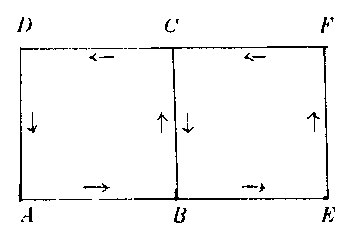
\includegraphics{chap02-vend-scan-01.eps}
\end{figure}

In general we say a complex of squares is coherently oriented if, whenever a side of a square occurs as the boundary of two squares, it occurs with opposite orientations. \emph{Every complex in the plane or sphere consisting of a finite number of squares can be coherently oriented}.

\textsc{Reference:} \citeauthor{Kelley0000}~[\ref{Kelley1}]\index{Kelley, J. L.}.


\skiptoctrue
\section*{Exercises}

1. If $\{A_{i}\}$ is a disjoint family of open sets, then
\begin{equation*}
\mathrm{Bd}\{\bigcup_{i}A_{i}\}\supset\bigcup_{i}\{\mathrm{Bd}A_{i}\}
\end{equation*}
with equality if $\{A_{i}\}$ is a finite family.

2. If $G$ is a region of the complex sphere and $A$ is a nonempty open subset of $G$ such that no boundary point of $A$ lies in $G$, then $A=G$.

\section{Mappings}\label{ch02:sec3}

\subsection{}\label{ch02:sec3A}
Let $X$ and $Y$ be topological spaces. A \emph{mapping form} $X$ \emph{into} $Y$ is a rule which assigns a unique element of $Y$ to each element of $X$. A mapping is also called a \emph{function}.

If $f$ is a mapping which assigns $y$ to $x$, we write $f:x\rightarrow y$ or $y=f(x),\,f(x)$ is the image of $x$ under $f$, or the value of $f$ at $x$. If every element of $Y$ is an image, we say $f$ is \emph{onto}. If every $y\in Y$ is the image of exactly one $x\in X,\,f$ is said to be one-to-one (1-1).

$X$ is the \emph{domain} of $f$. In general, the \emph{domain} of $f$ is the set of $x\in X$ to which $f$ assigns a value. The \emph{range} of $f$ is the set of images $f(X) = \{f(x)|x\in X\}$.


\subsection{}\label{ch02:sec3B}
If $g$ is a mapping from $Y$ to $Z$, the \emph{composition mapping}\index{composition mapping} $g \circ f$ is defined to be the rule which assigns to $x \in X$ the value $g(f(x))$. Obviously $g \circ f$ is defined on $X$ only if the domain of $g$ includes the range of $f$. The meaning of $h\circ g \circ f$, etc., is clear.


\subsection{}\label{ch02:sec3C}
The \emph{inverse image} $f^{-1}(y)$ of $y\in Y$ is the set of $x\in X$ such that $f(x)=y$. Similarly, by $f^{-1}(A)$ we denote the set of $x\in X$ such that $f(x)\in A$. Note that $f\circ f^{-1}(A)=A$ but in general $f^{-1}\circ f(A)\supset A$.

If $A,\,B$ are subsets of $Y$, we have
\begin{equation*}
 f^{-1}(A\cap\,B)=f^{-1}(A)\cap f^{-1}(B),\textstyle\,\qquad f^{-1}(A\,\bigcup\,B)=f^{-1}(A)\bigcup f^{-1}(B).
\end{equation*}
If $A,\,B$ are subsets of $X$, then
\begin{equation*}
\textstyle f(A\,\bigcup\, B)=f(A)\bigcup f(B),\qquad f(A\cap\,B)\subset f(A)\cap f(B).
\end{equation*}
These relations hold for arbitrary unions and intersections. If $A \subset
B$ then $f(A)\subset f(B)$. If $f(A)$ meets $B$, then $A$ meets $f^{-1}(B)$ and conversely. In general it is not true that
\begin{equation*}
f(A\cap B)=f(A)\cap f(B),
\end{equation*}
but this equation is correct if $f$ is 1-1.


\subsection{}\label{ch02:sec3D}
Suppose $f$ is a 1-1 mapping of $X$ on $Y$. Then $f^{-1}(y),\,y\in Y$, is a single point of $X$. Thus the rule which assigns $f^{-1}(y)$ to $y$ is a \emph{function}, called the inverse function and denoted by $f^{-1}$. Note that
\begin{equation*}
f \circ f^{-1}(y)=y,\quad y\in Y;\qquad f^{1}\circ f(x)=x,\quad x\,\in X.
\end{equation*}


\subsection{}\label{ch02:sec3E}
If $f$ is a mapping from $X$ to $Y$ and $A$ is a subset of $X$, the mapping with domain $A$ which sends $x$ into $f(x)$ is called the restriction\index{restriction} of $f$ to $A$ and is denoted by $f\,|\,A$.


\subsection{}\label{ch02:sec3F}
Let $f$ be a mapping of the topological space $X$ into the set $Y$. We introduce a topology in $Y$ by defining $A$ to be open in $Y$ if and only if $f^{-1}(A)$ is open in $X$. In particular, if $R$ is an equivalence relation in $X$, the set $S=R\backslash X$ (cf.~\ref{ch02:sec1B}) may be topologized in this way, $f$ being the mapping that assigns to $x \in X$ the equivalence class $Rx$ containing $x$. $S$ is called the \emph{quotient space}\index{quotient space} of $X$ modulo $R$ and the above topology is the \emph{topology induced by}\index{topology!induced} $f$.


\subsection{}\label{ch02:sec3G}
Various properties can be ascribed to the mapping $f$ of a topological
space $X$ into a topological space $Y$. The mapping $f$ is \emph{continuous}\index{mapping!continuous} provided $f^{-1}$ maps open sets on open sets. The mapping $f$ is \emph{open}\index{mapping!open} provided $f$ maps
open sets on open sets. The mapping $f$ is a \emph{homeomorphism} or \emph{topological
mapping} provided it is 1-1, open, and continuous. Then $X$ and $Y$ are said
to be \emph{homeomorphic}\index{mapping!homeomorphic}.

Two subsets $A\subset X,\,B \subset Y$ are homeomorphic if there is a 1-1 mapping of $A$ on $B$ which is open and continuous in the relative topologies of $A$ and $B$.

The restriction of a continuous function $f$ to any subset of its domain is still continuous. If $f$ is a homeomorphism from $A$ to $B$ and $g$ is the restriction of $f$ to $A_{1}\subset A$, then $g^{-1}$ may be defined as the restriction of $f^{-1}$ to $f(A_{1})$ and $g$ is a homeomorphism.

\begin{theorem*}
Let $f$ be a mapping of $X$ into $Y$. Let $X$ be assigned any topology and let $Y$ be assigned the topology induced by $f$ \emph{(cf. \ref{ch02:sec3F})}.
Then $f$ is continuous. If $f$ is \emph{1-1}, it is a homeomorphism.
\end{theorem*}


\begin{proof*}
\emph{A} open in $Y$ implies $f^{-1}(A)$ open in $X$, by definition. Hence $f$ is continuous. If $f$ is 1-1, $B$ open in $X$ implies $f^{-1}\circ f(B)$ open in $X$, since $f^{-1}\circ f(B) = B$. But this means $f(B)$ is open in $Y$. Hence $f$ is open.\:\:\:q.e.d.
\end{proof*}

\subsection{}\label{ch02:sec3H}
\emph{The continuous image of a compact set is compact. The continuous
image of a connected set is connected}.


\subsection{}\label{ch02:sec3I}
An \emph{arc}\index{arc} is a continuous image in a topological space of the interval
[0, 1]. We write $\gamma : t \rightarrow f(t),\, 0 \leqq t\leqq 1;\, f(0)$ is the initial point, $f(1)$ the
terminal point of the arc $\gamma$. A \emph{Jordan arc}\index{Jordan arc} is a topological image of [0, 1].

A \emph{Jordan curve}\index{Jordan curve} or \emph{simple closed curve}\index{simple closed curve} is a topological image of a circle.

A topological space is said to be \emph{arcwise connected}\index{arcwise connected} if any two points in the space are the endpoints of a Jordan arc. An arcwise connected space is connected. The euclidean spaces are arcwise connected.


\subsection{}\label{ch02:sec3J}
A region of the complex sphere is said to be simply connected\index{simply connected} if it is
a topological image of the whole sphere or the once punctured sphere. The
boundary of a simply connected region is either empty or else consists of a single continuum (\ref{ch02:sec2I})---(cf. M. H. A. [\citeauthor{Newman0000}~\ref{Newman1}\index{Newman, M. H. A.}, p. 144]). An equivalent
definition; $G$ is a simply connected region if every simple closed curve in $G$ can be shrunk continuously to a point of $G$. The interior of a simple closed curve is a simply connected region; also the exterior.

A region of the sphere will be said to have \emph{connectivity} $n\ (2 \leqq
n \leqq \infty)$ if it is a homeomorph of the region obtained by deleting $n$ distinct continua from the sphere.


\subsection{}\label{ch02:sec3K}
A 2-dimensional \emph{manifold}\index{manifold} or \emph{surface} is a connected Hausdorff space in which every point has an open neighborhood that is homeomorphic with an open set in the euclidean plane. If $S$ is a surface and $G$ a region in $S$, then $G$ is itself a surface. Indeed, if $x \in G$ then $x \in S$ and lies in a neighborhood $U$ associated with a homeomorphism $\Phi$. Then $U \cap G$ is an open neighborhood of $x$ in $G$ and the restriction of $\Phi$ to this neighborhood is the
associated homeomorphism. Familiar examples of surfaces are the plane,
the sphere, and the torus.

A surface is arcwise connected, and each of its points has a compact, connected
neighborhood.

\textsc{References} \citeauthor{Kelley0000}~[\ref{Kelley1}]\index{Kelley, J. L.}; \citeauthor{Ahlfors0000a}\index{Ahlfors-Sario} [\ref{Ahlfors}].


\skiptoctrue
\section*{Exercises}

1. Let $X$ be a compact space, $Y$ a space, and $f$ a 1-1 mapping of $X$ onto $Y$. If $f$ is continuous, it is a homeomorphism.

2. Any two points of a region $G$ in a euclidean space can be joined by a Jordan arc which lies in a compact subset of $G$.

\section{Hilbert Space}\label{ch02:sec4}

\subsection{}\label{ch02:sec4A}
A Hilbert space is first of all a complex vector space\index{vector space}, which we now
define.

A set of elements $H = \{x,y,z,\cdots\}$ is a complex vector space if there is defined in $H$ a sum $x + y$ and a scalar multiple $\alpha x$, which satisfy the following postulates for all $x,y,z \subset H$ and all complex numbers $\alpha,\,\beta$:

A1. $x+y \in H;\, (x+y) + z=x+(y+z); x+y=y+x$.

A2. There is an element $0 \in H$ such that $0 + x = x$.

A3. There is an element $-x \in H$ such that $x + (-x) = 0$.

A4. $\alpha x \in H;(\alpha +\beta)x=\alpha x+\beta x; \alpha(x+y)=\alpha x + \alpha y;\,(\alpha\beta)x=\alpha(\beta x)$.

A5. $1\cdot x=x$.


\subsection{}\label{ch02:sec4B}
In $H$ we can sometimes define a norm function, denoted by $\Vert x\Vert$ for which the following hold:

B1. $\Vert x\Vert \geqq 0, \, \Vert x\Vert=0$ if and only if $x =0$,

B2. $\Vert \alpha x\Vert=|\alpha|\cdot\Vert x\Vert$,

B3. $\Vert x+y\Vert\leqq\Vert x\Vert + \Vert y\Vert$.

\noindent With this norm $H$ becomes a \emph{normed vector space} (or a normed linear space). Clearly $H$ is a metric space with the metric $\rho(x,\,y)=\Vert x -y\Vert$. By $x_{n}\rightarrow x$ we mean $\Vert x_{n}- x\Vert \rightarrow
0$: this is called convergence in norm.


\subsection{}\label{ch02:sec4C}
A \emph{scalar product}\index{scalar product} in $H$ is a complex-valued function of two elements
$x,y$, denoted by $(x,y)$ and possessing the following properties:

C1. $(x,y)=\overline{(y,x)},$

C2. $(x,x) \geqq 0;(x,x)=0$ if and only if $x = 0$,

C3. $(\alpha x + \beta y ,z) = \alpha(x,z) + \beta(y,z)$.

\noindent (Here $\overline{a}$ is the complex conjugate of $a$.) From these axioms we deduce \emph{Schwarz's inequality}:
\begin{equation}\label{ch02:eqn1}
|(x,y)|\leqq\Vert x\Vert\cdot\Vert y\Vert.
\end{equation}

A vector space possessing a scalar product becomes a normed space on
setting $\Vert x\Vert = (x, x)^{1/2}$, for Schwarz's inequality\index{Schwarz's inequality} implies B3. This norm is
said to be derived from the scalar product.


\subsection{}\label{ch02:sec4D}
\textsc{Definition}. A Hilbert space\index{Hilbert space} is a complex vector space which possesses a scalar product and which is complete in the norm derived from the scalar product.

The last condition means that if $(x_{n})$ is a sequence in a Hilbert space such that $\Vert x_{m}- x_{n}\Vert\rightarrow 0$ as $m,\,n \rightarrow\infty$ (Cauchy sequence), there exists an element $x$ of the Hilbert such that $\Vert
x_{n}- x\Vert \rightarrow 0,\,n \rightarrow \infty$.

The complex euclidean space of finite dimension $n$ is an example of a Hilbert space. So is $l_2$, the space of infinite vectors $x =(x_{1},\,x_{2},\,\cdots)$ which are such that $\sum_{i}|x_{i}|^{2}$ converges. (The $x_i$ are complex numbers.) Let $y= (y_{1},\,y_{2},\,\cdots)$. Sum and scalar multiples are
defined in the obvious way and scalar product by $(x,y) = \sum{_{i}}x_i\overline{y}_i$.

Another Hilbert space of importance to us is $L_{2}(\mathscr{D})$. Here $\mathscr{D}$ is a region of the complex sphere and $L_{2}(\mathscr{D})$ is the space of complex-valued functions $f(z)$ which are Lebesgue measurable in $\mathscr{D}$ and are such that
\begin{equation*}
 \iint\limits_{\mathscr{D}} |f(z)|^{2} dx\, dy\,<\infty,\qquad z=x+iy
\end{equation*}
the integral being a Lebesgue integral (cf. \ref{ch02:sec13C}). We set
\begin{equation*}
(f,g)= \iint\limits_{\mathscr{D}} f(z)\overline{g(z})dx\,dy.
\end{equation*}

We can also construct a Hilbert space using a positive weight function $\omega(z)$ by defining
\begin{equation*}
(f,\,q)=\iint\limits_{\mathscr{D}} f(z)\overline{g(z})\omega(z)dx\,dy.
\end{equation*}

In the last two Hilbert spaces the elements of the space are not the functions
$f(z)$ but rather equivalence classes $(f)$. Two functions are in the same
equivalence class if they differ on a set of Lebesgue measure 0 (possibly
the null set).


\subsection{}\label{ch02:sec4E}
Let $x_{1},\,x_{2},\,\cdots$ be elements of a Hilbert space $H$. An expression of the form $\alpha_{1}x_{1}+\alpha_{2}x_{2}+\cdots+ \alpha_{k}x_{k},\,\alpha_{i}=$
complex number, is called a finite linear combination of $x_{1},x_{2},\cdots,x_{k}$.
A subset of $H$ which includes all finite
linear combinations of its elements is called a \emph{linear manifold}\index{linear manifold}.
A \emph{subspace}\index{subspace} of $H$ is a subset of $H$ which is itself a Hilbert space under the same addition and scalar product defined in $H$. A subspace is evidently a linear manifold.

Let $M$ be a linear manifold in $H$. Adjoin to $M$ the limits of all convergent
sequences in $M$. The resulting set is the closure of $M$, denoted as usual by $\bar{M}$. It is seen at once that $\bar{M}$ is complete in the norm of $H$. Hence, \emph{the closure of a linear manifold is a subspace}, the other requirements being trivially verified.

Two elements $x, y$ of $H$ are \emph{orthogonal} if and only if $(x, y) = 0$. We write $(A, B) = 0$ to signify that $(x, y) = 0$ for $x \in A, y \in B,\, A$ and $B$ being subsets of $H$. Given a linear manifold $M$ we define $N = \{x \in H\,|\,(x, M) = 0\}$ and
call it \emph{the orthogonal complement}\index{orthogonal complement} of $M$. \emph{The orthogonal complement of a linear manifold is a subspace.}

Let $H_{1}$ be a subspace (rather than merely a linear manifold) of $H$ and $H_{2}$ its orthogonal complement. We have the important

\textsc{Decomposition Theorem.}\index{decomposition theorem}
$H =H_{1}\bigoplus H_{2}$, \emph{that is, each} $x\in H$ \emph{can be written uniquely in the form} $x_{1}+x_{2}$, \emph{where} $x_{1}\in H_{1}$ \emph{and} $x_{2}\in H_{2}$.


\subsection{}\label{ch02:sec4F}
Let $A =\{x_{1},\,x_{2},\,\cdots\}$ be a subset of $H$. $B$ is said to be \emph{spanned by} $A$ if $B$ is contained in the set of all finite linear combinations of elements of $A$. A \emph{finite-dimensional Hilbert space}\index{Hilbert space!dimension of} is one which is spanned by a finite subset of its elements. \emph{In a finite-dimensional Hilbert space every linear manifold is closed, that is, is a subspace},

The elements $x_{1},\,x_{2},\,\cdots,\,x_{n}$ of $H$ are said to be \emph{linearly independent over the complex field} if the relation $\alpha_{1}x_{1}+\alpha_{2}x_{2}+\cdots+\alpha_{n}x_{n}=0$ implies $\alpha_{1}=\alpha_{2}=\cdots=\alpha_{n}=0$. A subset $A \subset
H$ which consists of linearly independent elements and spans $H$ is called a \emph{basis}\index{Hilbert space!basis for}. \emph{All bases of} $H$ \emph{contain the same cardinal number of elements}. This number, which is therefore characteristic of $H$, is called the \emph{dimension} of $H$. The space $\{0\}$, consisting of the zero element alone, is arbitrarily assigned the dimension $0$. \emph{Every element of} $H$ \emph{has a unique expression as a linear combination of basis elements. If} $H$ \emph{is of dimension} $n$, \emph{every set of} $n$ \emph{linearly independent elements is a basis}.

\begin{theorem*}
From $H=H_{1}\bigoplus H_{2}$ follows $\dim H= \dim H_{1}+\dim H_{2}$.
\end{theorem*}

\textsc{Reference:} \citeauthor{Riesz0000}\index{Rieaz-Nagy} [\ref{Riesz}].


\section{Groups}\label{ch02:sec5}\index{group}

\subsection{}\label{ch02:sec5A}
The reader will know the definition of group, finite group, order of a group, and order of a group element. The group $G$ is called \emph{commutative} or \emph{abelian} if any two elements commute: $ab=ba$ for $a,\,b\in G$. The \emph{commutator}\index{commutator} of $a,\,b$ is $aba^{-1}b^{-1}$; it is equal to the identity if and only if $a,\,b$ commute.

A subset $H\subset G$ is a \emph{subgroup} of $G$ if the elements of $H$ form a group under the same multiplication as in $G$. A convenient test: $H$ is a subgroup if and only if $a,\,b\in H$ implies $ab^{-1}\in H$.

We introduce the following general notation. If $A,\,B$ are subsets of $G$---in particular $A$ or $B$ may be a single element---we write $AB$ to denote the set of all products $xy,\,x\in A,\,y\in B$.

Let $x$ and $y$ be called equivalent if $xy^{-1}\in H$. This equivalence relation partitions $G$ into disjoint classes, called \emph{left cosets}\index{coset}, of the form $Hx$. We have $G =\bigcup_{i} Hx_{i}$ where $\{x_{i}\}$ is a \emph{set of representatives} of the left cosets of $H$ in $G$. We write
\begin{equation*}
H\backslash G=\{Hx_{i}\},\qquad (H\backslash G)=\{x_{i}\}
\end{equation*}
in which $H$ always appears on the \emph{left}. Similarly the equivalence relation, $x$ equivalent to $y$ if and only if $x^{-1}y\in H$, divides $G$ into \emph{right cosets} $xH$, and
\begin{equation*}
G/H=\{x_{i} H\},\qquad (G/H)=\{x_{i}\}
\end{equation*}
$H$ always appearing on the \emph{right}. The cardinal number of left and right cosets is the same; this number (finite or infinite) is called the \emph{index} of $H$ in $G$ and is denoted by $[G: H]$.

If $xH=Hx$ for each $x$ in $G$, we say $H$ is a \emph{normal} or \emph{invariant} subgroup. This condition is equivalent to $xHx^{-1}=H$ for all $x$. Suppose we know only that $xHx^{-1}\subset H$ for each $x$. Since $H=x^{-1}(xHx^{-1})x\subset
x^{-1} Hx \subset H$, we can conclude that $x^{-1}Hx =H$. Hence $H$ \emph{is a normal subgroup of}\index{normal subgroup} $G$ \emph{provide}
\begin{equation*}
xHx^{-1}\subset H\ \mathit{for\ each}\ x\in G.
\end{equation*}

Let $N$ be a normal subgroup of $G$. The collection of cosets $\{xN\}$ becomes a group under the multiplication $xN\cdot yN=xyN$. This group, denoted by $G/N$, is called the factor (or quotient)\index{group!factor (=quotient)} group of $G$ modulo $N$; it is obviously the same group as $N\backslash G$.

Suppose $\{H_{i}\}$ is an indexed family of subgroups of $G$. We define two new groups: the \emph{intersection}\index{group!intersection of\_\_\_s} $\cap_{i} H_{i}$ and the \emph{union}\index{group!union of \_\_\_s} $\bigcup_{i} H_{i}$. The first consists of the $x\in G$ which lie in every $H_{i}$; the second, of all finite products $x_{1}\cdots x_{k}$, where each $x_{i}$ belongs to some $H_{j}$.

Let $X=\{x_{1},\,x_{2},\,\cdots\}\subset G$. By $\{X\}$ we shall mean the set of all finite words $y_{1}y_{2}\cdots y_{t}$, where each $y_{i}$ is an $x_{j}$ or an $x_{j}^{-1}$. The elements of $\{X\}$ form a group, a subgroup of $G$, called the \emph{group generated by}\index{group!generators of a} $X$. If $\{X\}=G$, we say that $X$ is a \emph{system of generators}\index{system of representatives} of $G$. Trivially, $G$ itself is a system of generators of $G$, but there may be proper subsets of $G$ that generate $G$.


\subsection{}\label{ch02:sec5B}
Let $f$ be a mapping of $G$ into a group $G^{\prime}$ which has the property that $f(xy)=f(x)f(y)$ for each pair $x,\,y\in G$. We call $f$ a homomorphism\index{homomorphism}\index{homomorphism theorem} of $G$ into $G^{\prime}$; if the range of $f$ is $G^{\prime}$ itself, we speak of a homomorphism \emph{onto} $G^{\prime}$. If $e,\,e^{\prime}$ are the identities of $G$ and $G^{\prime}$, respectively, then $f(e)=e^{\prime}$. The \emph{kernel} of $f$ is the set $N=f^{-1}(e^{\prime})$.

Let $f:G\rightarrow G^{\prime}$ be a homomorphism which is 1-1. We then say $f$ is an \emph{isomorphism}\index{isomorphism} and also that $G$ and $G^{\prime}$ are \emph{isomorphic}.

\begin{theorem*}
If $f$ is a homomorphism of $G$ onto $G^{\prime}$ with kernel $N$, then $N$ is a normal subgroup of $G$, and $G^{\prime}$ is isomorphic to $G/N$. Conversely, if $N$ is a normal subgroup of $G$, there is a homomorphism $f$ of $G$ onto $G/N$ with kernel $N$. The mapping $f$ is defined by $f(x)=xN$.
\end{theorem*}

The mapping $f$ is called the quotient map of $G$ on $G/N$.


\subsection{}\label{ch02:sec5C}
An important class of infinite groups are the \emph{free groups}\index{free group}\index{group!free} (\citeauthor{Hall0000}~[\ref{Hall1}\index{Hall, Marshall}, pp. 91--93, 311--312]). Let $S =\{s_{i}\}$ be a collection of symbols; define the new symbol $s_{i}^{-1}$; finally set $s_{i}^{1}=s_{i}$. A \emph{word}\index{word} is either the empty word containing no symbols (written 1) or a symbol
\begin{equation*}
f=a_{1}\,a_{2}\cdots a_{t},\qquad t\ \mathrm{finite}
\end{equation*}
where each $a_{i}$ is an $s_{j}^{\varepsilon},\,\varepsilon=\pm\, 1$. Two words are equivalent if one can be obtained from the other by the deletion or insertion of a finite number of symbols of the form $s_{j}^{\varepsilon}s_{j}^{-\varepsilon}$. This is a true equivalence relation and we denote by $[f]$ the equivalence class containing $f$. The word $f$ is reduced if it is 1 or if it contains no sequence $a_{i}\ a_{i+1},\, i=1,\,\cdots,\,t -1$, of the form $s_{j}^{\varepsilon}s_{j}^{-\varepsilon}$.
It can be shown that each equivalence class contains one and only one reduced word.

We can define a multiplication in the equivalence classes by setting $[f][g]=[ fg]$. Under this multiplication, which is well-defined, the equivalence classes form a group, the identity being the class [1]. We call this group the \emph{free group} $F$ generated by $S$.

The importance of free groups is underlined by the following result.

\begin{theorem*}
Let $G$ be generated by the set $X=\{x_{i}\}$ and let $F$ be the free group generated by $S=\{s_{i}\}$, where $S$ has the same cardinal number as $X$. Then the mapping $s_{i}\rightarrow x_{i}$, all $i$, is a homomorphism of $F$ onto $G$.
\end{theorem*}

In other words, every group defined by generators is a factor group of a free group with the same number of generators.

Let the free group $F$ generated by $S$ be also generated by a set $X=\{x_{i}\}$. We say $X$ is a \emph{system of free generators}\index{free generators} provided no reduced word in the $x_i$ is equal to 1 except 1 itself. It is implicit in the definition of a free group that $S$ is a system of free generators for the free group $F$ which it generates.

J. Nielsen (also O. Schreier) proved the fundamental

\begin{theorem*}
A subgroup of a free group is itself a free group.
\end{theorem*}

The concept of a free group enables us to define the \emph{relations}\index{relations in a group} in an arbitrary group accurately. Let $G$ be a group generated by $X=\{x_{1},x_2,\,\cdots,\,x_{r}\}$. Let $F$ be the free group generated by free generators $S=\{s_{i}\}$, where $S$ and $X$ are in 1-1 correspondence, and let $N$ be the kernel of the homomorphism $f:F\rightarrow G$ given by $s_{i}\rightarrow x_{i}$. Then if $s_{i_{1}}^{\varepsilon_{1}}\cdots s_{i_{k}}^{\varepsilon_{k}}$ is a word in $N$, it maps into a word $\mathbf{R} =x_{i_{1}}^{\varepsilon_{1}}\cdots x_{i_{k}}^{\varepsilon_{k}}$ in $G$, and $\mathbf{R} =e$ since $N$ maps into $e$ under $f$. An equation of the form
\begin{equation*}
\mathbf{W}=x_{i_{1}}^{\varepsilon_{1}}\cdots x_{i_{k}}^{\varepsilon_{k}} =e
\end{equation*}
is called a \emph{relation in} $G$. Every relation is obtained by the above process since $f^{-1}(\mathbf{W})=f^{-1}(e)\in N$.

Because{\def\thefootnote{$^{\ast}$}\footnote{Cf. Note to Chapter~\ref{ch02:chap02}, p. 399.}} $N$ is a subgroup of the free group $F$, it is itself a free group and has a system of free generators $\Re=\{N_{1},\,N_{2},\,\cdots,\,N_{h}\}$. The elements of $\Re$ are independent in the sense that no reduced word in the $\{N_{j}\}$ is equal to 1. The words
\begin{equation*}
\Re =\{\mathbf{R}_{j}\},\qquad j=1,\,\cdots,\,h
\end{equation*}
which are the images of $\{N_{j}\}$ under the homomorphism $f$, are said to form a \emph{basis for the relations in}\index{relations in a group!basis for} $G$; they are also called \emph{defining} or \emph{generating relations} of $G$. A basis is characterized by two properties:

1) every relation $\mathbf{R}$ in $G$ is a consequence of relations in $\Re$, which means that for some $T_{i}\in G$.
\begin{equation*}
\mathbf{R}= \prod_{i=1}^{k} T_{i}\mathbf{R}_{\nu_{i}}^{\varepsilon_{i}},T_{i}^{-1},\qquad
1\leqq \nu_{i} \leqq h
\end{equation*}

2) no relation in $\Re$ is a consequence of the remaining relations in $\Re$.

A statement $G = \{X; \Re\}$ of a system of generators and a basis for the
relations of $G$ is called a \emph{presentation}\index{group!finitely presented} of $G$; it is finite if both $X$ and $\Re$ are finite sets.

Closely related to the free group is the \emph{free product}\index{free product of groups} of a family of groups $\{G_{i}\}$. Form all the finite words $a_{1}a_{2}\cdots a_{t}$. where each $a_i$ belongs to some $G_{j}$. Two words are equivalent if one
can be obtained from the other by applying the following operations a finite number of times: \eqref{ch02:eqn1} omitting $a_{i}$ if it is the identity of the group to which it belongs, \eqref{ch02:eqn2} replacing $a_{i}a_{i+1}$
by  $a^{\ast}$ if  both $a_{i}$ and $a_{i+1}$ are in the same $G_{j}$ and
$a_{i}a_{i+1}=a^{\ast}$. We agree to set the identities of the groups $G_{j}$ all equal to 1, the empty word. A word $a_{1}\cdots a_{t}$ is reduced if it is 1 or if the above operations have been carried out
as far as possible. Each equivalence class of words can be shown to contain
one and only one reduced word, and we can multiply classes exactly as before. The set of all equivalence classes is called the free product of $\{G_{j}\}$
and is denoted by
\begin{equation*}
^{\ast} \prod_{j} G_{j}.
\end{equation*}

It would seem that if each $G_{j}$ is a subgroup of a group $G$, the free product of $\{G_{j}\}$ is the same as the union of $\{G_{j}\}$ -- cf. \ref{ch02:sec5A}. Indeed there is a homomorphism of $^{\ast} \Pi_{j} G_{j}$ on $\bigcup_{j}G_{j}$ (\citeauthor{Hall0000}~[\ref{Hall1}, p. 312]). But the two need not be
isomorphic. For example, suppose $G = \{a, b,\cdots\}$ is a group having the relation $aba^{-1}b = 1$. Let $H_{1},H_{2}$ be the cyclic subgroups of $G$ generated by $a$ and $b$, respectively, $a \neq b^{-1}$. Then $aba^{-1}b$, or rather the equivalence class containing it, is an element of $H_{1} \ast
H_{2}$ different from the identity. In $H_{1}\bigcup H_{2}$, however, $aba^{-1}b=1$.
 

\subsection{}\label{ch02:sec5D}
An important example\index{principal circle} of a group is a \emph{group of matrices of order} $n$,
that is, a collection of $n \times n$ matrices which forms a group under the operation of matrix multiplication. The identity of the group is the unit matrix $I = (\delta_{ij}),\ i,j = 1,\cdots,n$. Clearly the set of all \emph{nonsingular} matrices of order $n$ is a group $\Omega_n$. To check that any given collection $G$ of nonsingular
matrices of order $n$ is a group (i.e., is a subgroup of $\Omega_{n}$), we have only to verify that $M_{1}M_{2}^{-1}= G$ whenever $M_{1}, M_{2} \in G$. For example, the set of all nonsingular matrices of order $n$ and determinant 1 is obviously a group.


\subsection{}\label{ch02:sec5E}
Let $A$ be a set and $f$ a 1-1 mapping of $A$ on itself. The set $\Delta$ of all such mappings forms a group under composition of mappings. That is,
the product of two elements $f,g\in \Delta$ is the mapping $f\circ g$. Associativity is immediately checked. The identity mapping $e$, defined by $e(x) = x$ for
each $x\in A$, is 1-1 and is in $\Delta$, and so is $f^{-1}$, the inverse of $f$. Hence $\Delta$ is a group, a \emph{transformation group}\index{transformation group} on $A$.

Let $H$ be a collection of 1-1 mappings of $A$ which contains with $f, g$ also $f \circ g^{-1}$. Then $H$ is a group, a subgroup of $\Delta$.


\subsection{}\label{ch02:sec5F}
A homomorphism of a group $G$ into a group of matrices $M$ is called a
\emph{representation}\index{representation} of $G$. If the homomorphism is an isomorphism, the representation is called \emph{faithful}. By definition the degree of the representation is the order of $M$.

Let $h_{1} : x \rightarrow h_{1}(x); h_{2}:x\rightarrow h_{2}(x)$ be two representations of $G$ of the same degree. The representations are called \emph{equivalent} if there is a matrix $a$, not depending on $x$, such that $ah_{1}(x)a^{-1} = h_{2}(x)$ for each $x\in G$.

Representations are of value because the matrix group $M$ permits calculation
whereas $G$ is abstract.


\skiptoctrue
\section*{Exercise}

1. Let $H$ be a subgroup of $G$ of finite index $\mu$. If $x \in G$, then $x^{e}\in H$ for some $e$ in the range $1 \leqq  e \leqq \mu$.

\textsc{References:} M. \citeauthor{Hall0000}~[\ref{Hall1}]\index{Hall, Marshall}; W. \citeauthor{Magnus0000}~[\ref{Magnus1}]\index{Magnus}.

\section{Topological Groups}\label{ch02:sec6}

\subsection{}\label{ch02:sec6A}
\emph{A} \emph{topological group}\index{topological group} is a set $G$ which is both an abstract group and a
topological space and in which the following condition is satisfied (continuity
of multiplication): $x_{n}y_{n}^{-1}\rightarrow  xy^{-1}$ whenever $x_{n}\rightarrow
x,\,y_{n}\rightarrow y$ with $x_{n},y_{n},x,y\in G$. The products $x_{n}y_{n}^{-1},xy^{-1}$
 are defined because $G$ is a group, and convergence is defined because $G$ is a space.

A topological group $G$ is called \emph{discrete}\index{topological group!discrete} if none of its elements is an accumulation point of the space $G$. Equivalently we may say that $G$ is discrete if and only if it contains no sequence of distinct elements converging
to a group element.

Any abstract group $H$ may be topologized so as to become a discrete topological group by defining the family of open sets in $H$ to be the family of all subsets of $H$. However, this topology gives no significant information,
nor is it necessarily the only topology that can be put on an abstract group.
Cf. M. \citeauthor{Hall0000}~[\ref{Hall2}].


\subsection{}\label{ch02:sec6B}
In this book we shall be concerned almost entirely with matrix groups or, more accurately, with the matrix representations of groups. A matrix group may be topologized in the following way. Let $G = \{V\}$ be a group of
matrices $V = (a_{jk}),\ j , k = 1, 2,\cdots, n$, of order $n$ with complex entries $a_{jk}$. We make $G$ a metric space by defining the distance $\rho(V_{1},V_{2})\,=\max \{| a_{jk}^{(1)} - a_{jk}^{(2)}|,j,k=1,2,\cdots,n\}$ between any pair of
matrices $V_{1},V_{2}$ in $G$. Then convergence in $G$ is equivalent to elementwise convergence: $V_{r}\rightarrow V, r \rightarrow\infty$, if and only if $a_{jk}^{(r)}\rightarrow
a_{jk},r \rightarrow \infty$, for each $j, k = 1, 2,\cdots,n$.


\subsection{}\label{ch02:sec6C}
The definition of discreteness\index{topological group!discrete} of a topological group (\ref{ch02:sec6A}) can be put into a more convenient form when the group is a group of matrices.

\setcounter{footnote}{0}
\begin{theorem*}
A matrix group $G$ is discrete if and only if it contains no convergent sequence of distinct matrices.\footnote{The point of the theorem is that the sequence is not required to converge to a group elements.}
\end{theorem*}

\begin{proof*}
Suppose $(V_{n})\in G$ is a sequence of distinct matrices such that $V_{n}\rightarrow V$, where $V$ is a nonsingular matrix (which may or may not belong to $G$). Then $V_{n}^{-1} \rightarrow V^{-1}$ and $T_{n}=V_{n}^{-1}V_{n+1}\rightarrow V^{-1}V=I$. Furthermore infinitely many $T_{n}$ are distinct. Otherwise $T_{n}=I$ for $n>N$, which implies $V_{n}=V_{n+1}$ for $n>N$, contradicting the assumption that the $\{V_{n}\}$ are distinct. Thus there is a subsequence $(T_{p})$ of distinct matrices in $G$ such that $T_{p}\rightarrow I$ and so $G$ is not discrete. On the other hand, if $G$ is not discrete, it contains a convergent sequence, namely, a sequence converging to a group element.\:\:\:q.e.d.
\end{proof*}

\textsc{Reference:} \citeauthor{Pontrjagin0000}~[\ref{Pontrjagin1}]\index{Pontrjagin}.


\section{Analytic and Harmonic Functions}\label{ch02:sec7}

\subsection{}\label{ch02:sec7A}
A \emph{complex-valued function} $f(z)$ of a \emph{complex variable} $z$ is a mapping from a region of the complex sphere $\mathscr{Z}$ into $\mathscr{Z}$. We say $f$ is \emph{regular at} $z =a$ (finite), or $a$ is a \emph{regular point} of $f$, if for each $z$ in a disk $K:0\leqq|z -a|<\rho$, we have
\begin{equation}\label{ch02:eqn2}
f(z)=c_{0}+c_{1}(z-a)+c_{2}(z -a)^{2}+\cdots.
\end{equation}
$f$ is \emph{regular at} $\infty$ if $g(z)=f(1/z)$ is regular at 0. A \emph{regular} (analytic\index{analytic function|(}, holomorphic) \emph{function} is a function which is regular somewhere. A function regular at each point of a set $S$ is said to be regular in $S$. Since the series \eqref{ch02:eqn2} can be re-expanded about any point $b\in K$, a function regular at a point is regular in a region about that point.

Within $K,\,f$ is a \emph{continuous} mapping; unless $f$ is constant it is an \emph{open} mapping\index{analytic function!as open mapping} (\ref{ch02:sec3G}). Thus a nonconstant $f$ maps regions onto regions. From \eqref{ch02:eqn2} we deduce that $f$ has derivatives of every order which, moreover, can be obtained by term-by-term differentiation. In particular, the coefficients $c_{n}$ are expressible as derivatives of $f$ at the point $a$: the power series is a \emph{Taylor} series.

Conversely, every function which is differentiable in a region is regular at each point of the region (Cauchy-Taylor Theorem). Thus the regular functions are those which are differentiable in a region.

\emph{A function which is regular in a compact set} $S$ \emph{is bounded in} $S$.

The composition $f\circ g$ of two regular functions is regular where it is
defined.


\subsection{}\label{ch02:sec7B}
If $f$ is regular only in a deleted disk $0<|z-a|<\rho$, we have the representation by a \emph{Laurent series}:
\begin{equation}\label{ch02:eqn3}
f(z)=\sum\limits_{n=-\infty}^{\infty}c_{n}(z-a)^{n}.
\end{equation}
Suppose $c_{n}=0$ for $n<s$ but $c_{s}\neq0$: we say $f$ has order $s$ at $z=a$ and write $n(a,f)=s$. When $s<0$ we speak of a pole of order $-s$; when $s >0$, of a zero of order $s$. At a pole $f$ tends to the definite value $\infty$. On the other hand a function which is regular and \emph{bounded} in a deleted disk can be extended so as to be regular throughout the disk by defining its value at the center by continuity (Riemann's Theorem)\index{Riemann}.

A function which at every point of a region $\mathscr{D}$ is either regular or has a pole is said to be \emph{meromorphic in}\index{meromorphic} $\mathscr{D}$. \emph{The zeros and poles of} $f$ \emph{do not accumulate in any region where} $f$ \emph{is meromorphic}. In particular, a function which is meromorphic in $\mathscr{Z}$ has only a finite number of poles (since $\mathscr{Z}$ is compact) and so must be a rational function of $z$. By the same token $f$ is identically zero if it has infinitely many zeros in a compact region where it is regular. A function which is meromorphic in the finite complex plane has a countable
(possibly infinite) number of poles.

Returning to \eqref{ch02:eqn3} we say $f$ has an \emph{isolated essential singularity} at $z=a$ if the series contains infinitely many terms with negative exponents. The Weierstrass-Casorati Theorem tells us that in this case the image of an arbitrary neighborhood of $a$ is dense in $\mathscr{Z}$, in other words, that $f$ is indeterminate at $a$. This theorem, moreover, is true even if $a$ is an accumulation point of poles of $f$ (cf. [\citeauthor{Dienes0000}~\ref{Dienes1}\index{Dienes}, p. 231f]).


\subsection{}\label{ch02:sec7C}
\textsc{Principle of the Maximum.}\index{maximum principle} Let $f$ be regular in a region $\mathscr{D}$. Unless $f$ is constant, $| f |$ does not attain its maximum value at an interior point of $\mathscr{D}$.

The result follows easily from the fact that $f$ is an open mapping.


\subsection{}\label{ch02:sec7D}
A \emph{path} $l$ is the image of the closed unit interval by a \emph{differentiate} homeomorphism.\footnote{This is a homeomorphism which is given parametrically by a pair of continuously differentiate functions. A path is always of finite length.} The integral of $f$ over the path $l$ is defined as soon as $f$ is continuous on $l$. When the path is a simple closed curve $C$, the symbol $\int_{C}f$ indicates an integration in the \emph{positive sense}, i.e., $C$ is described so that its interior always lies to the left. We can also integrate over a finite number of simple closed curves that make up the boundary of a region $\mathscr{D}$; each curve is then described so that $\mathscr{D}$ lies to its left.

The integral of a regular function $f$ over a simple closed curve vanishes if the curve and its interior consist entirely of regular points of $f$. It is therefore possible in a \emph{simply connected} region $\mathscr{D}$ to define the integral of a regular function:
\begin{equation*}
F(z)=\int_{z_{0}}^{z}f(w)dw.
\end{equation*}
$F$ is itself regular in $\mathscr{D}$ and $F^{\prime}=f$.

\emph{Cauchy's Integral Formulas:} For $n$ an integer,
\begin{equation}\label{ch02:eqn4}
f^{(n)}(z)=\frac{n!}{2\pi i}\int_{C_{1}}\frac{f(w)dw}{(w-z)^{n+1}};\qquad c_{n}=\frac{1}{2\pi i}\int_{C_{2}}\frac{f(w)dw}{(w-a)^{n+1}}
\end{equation}
$C_{1},\,C_{2}$ being simple closed curves in $\mathscr{D}$ which surround $z$ and $a$, respectively.

\emph{Integral depending on a parameter:}

\begin{theorem*}
Let $f(z,\,w)$ be continuous in $(z, w)$ when $z\in \mathscr{D}$ \emph{(}region\emph{)} and $w \in C$ \emph{(}path\emph{)}, and let $f$ be regular in $\mathscr{D}$
for each $w \in C$. Then $F(z) = \int_{C} f(z, w)dw$ is regular in $z$ for
$z\in \mathscr{D}$, and $F^{\prime}(z) = \int_{C} (\partial f /\partial z)dw$.
\end{theorem*}


\subsection{}\label{ch02:sec7E}
Let $F$ be regular in a bounded or unbounded region $\mathscr{D}$ except at a finite number of points. If $F^{\prime}=f$, we call $dF=fdz$ a \emph{differential}\index{differential} in $\mathscr{D}$. The residue of $dF$ at $z=a$ is the coefficient $c_{-1}$ of the Laurent expansion \eqref{ch02:eqn3} of $f$ about $a$; it can be different from 0 only at points where $f$ is not regular. The Residue Theorem states that when $C$, the boundary of $\mathscr{D}$, is the union of a finite number of simple closed curves,
\begin{equation}\label{ch02:eqn5}
\sum\limits_{\mathscr{D}} \mathrm{Res}\, d\,F =\frac{1}{2\pi i}\int_{C} d\,F,
\end{equation}
the integration being always in the positive sense. If $\mathscr{D}$ is the
whole sphere (in which case $f$ is rational), the sum of the residues is
zero.

The order of $dF$ at $z=a$, written $n(a,\,F)$, is defined to be the order
of $f$ at $a$---cf. \eqref{ch02:eqn3}. We have
\begin{equation}\label{ch02:eqn6}
\sum\limits_{n \in \mathscr{D}} n(a,\,dF)=\frac{1}{2\pi i}\int_{C}\frac{f^{\prime}(\zeta)}{f(\zeta)}\,d\zeta;
\end{equation}
in particular, the sum of the orders of a rational function is zero.


\subsection{}\label{ch02:sec7F}
Let $f_{n}(z),\,n=1, 2,\cdots$, be continuous in a region $\mathscr{D}$ and converge uniformly in $\mathscr{D}$ to $f(z)$. Then $f$ is continuous in $\mathscr{D}$ and
\begin{equation*}
\int_{l}f(\zeta)d\zeta= \lim_{n\rightarrow\infty}\int_{l} f_{n}(\zeta)d\zeta,
\end{equation*}
$l$ being a path lying in $\mathscr{D}$. If each $f_{n}$ is regular in $\mathscr{D}$ and the convergence is uniform on compact subsets of $\mathscr{D}$, then $f$ is regular in $\mathscr{D}$, i.e., \emph{the uniform limit of regular functions is regular}. Moreover,
\begin{equation*}
f_{n}^{(k)}(z)\rightarrow f^{(k)}(z),\qquad n \rightarrow\infty
\end{equation*}
for $k=1, 2,\cdots$, as may be proved by application of \eqref{ch02:eqn4}. This is Weierstrass'\index{Weierstrass} theorem;\index{Weierstrass' theorem} it may be expressed as a theorem on term-by-term integration of a uniformly convergent series.

\textsc{Vitali's theorem}. Let $\{f_{n}(z)\}$ be\index{Vitali's theorem} regular and uniformly bounded\footnote{I.e., $| f_{n}(z)| < M$ for all $n$ and all $z$ in $\mathscr{D}$} in a region $\mathscr{D}$ and let $f_{n}(z)$ converge at each point of a compact subset
 of $\mathscr{D}$. Then $f_{n}(z)$ converges uniformly on compact subsets of $\mathscr{D}$ to a function regular in $\mathscr{D}$.

\textsc{Montel's theorem}. From a family\index{Montel}\index{Montel's theorem} of regular functions uniformly bounded in a region $\mathscr{D}$
we can extract a sequence converging uniformly on compact subsets of $\mathscr{D}$.


\subsection{}\label{ch02:sec7G}
The series \eqref{ch02:eqn2} converges inside the largest disk $K$ about $a$ which lies in a region $\mathscr{D}$ where $f$ is regular, but $f$ may be regular outside $K$. Hence the series may not provide an algorithm for calculating all the values of $f$. The method of \emph{analytic continuation}\index{analytic continuation}, introduced by Weierstrass, gets around the difficulty. Denote the series \eqref{ch02:eqn2} by $P(a)$ and call it a \emph{function element}. Each function element is associated with a disk $K$ within which the series converges. If it is possible to find function elements $P(a_{i}),\ a_{0}=a,\,a_{1},\,a_{2},\,\cdots,\,a_{n}=b$, with associated disks $K_{i}$ such that $a_{i}\in K_{i-1}$, we say that the set $\{P(a_{i}),\ i=0,\,1,\,\cdots,\,n\}$ forms an analytic continuation of $f$ from $a$ to $b$. \emph{The analytic function} $f$ \emph{in the sense of Weierstrass} is the collection of all function elements obtained from any given function element by this process.

\emph{Two analytic functions which have a single function element in common are identical; an analytic function is completely determined by one of its function elements. This is the Principle of Analytic Continuation}.

It is possible we may obtain two different function elements $P_{1}(b),\,P_{2}(b)$ by continuation, from a given element along different chains of disks leading from $a$ to $b$. Then $f$ is a \emph{many-valued function}. Unfortunately, according to our definition in \ref{ch02:sec3A}, a many-valued function is not a function. A function in the sense of our original definition is often called a \emph{single-valued} or \emph{uniform} function.

An important sufficient condition for uniformity is given by the fundamental

\textsc{Theorem of Monodromy.}\index{Monodromy Theorem}  \emph{Let a be a point of a simply connected region} $\mathscr{D}$. \emph{Let} $f$ \emph{be regular at a and let it be possible to continue} $f$ \emph{analytically to any
point of} $\mathscr{D}$. \emph{Then} $f$ \emph{is uniform in} $\mathscr{D}$.


\subsection{}\label{ch02:sec7H}
Among the common many-valued functions are the logarithm\index{logarithm of zero-free function} and the power function. We define
\begin{equation}\label{ch02:eqn7}
\log z=\log|z|+i\,(\arg z\,+2k\pi),\qquad k =0,\,\pm\, 1,\,\pm\, 2,\,\cdots.
\end{equation}
We can construct a single-valued ``branch'' of the logarithm\index{branch of logarithm} by fixing $k$
and restricting $\arg z$. In this book we agree that always, unless otherwise stated, $\log z$ is defined by \eqref{ch02:eqn7} with $k=0$ and
\begin{equation}\label{ch02:eqn8}
-\pi\leqq\arg z<\pi.
\end{equation}
The function thus obtained is single-valued and continuous in the plane deleted by the negative real axis.

When we use an integration formula like
\begin{equation*}
\int_{a}^{b}dz/z=\log b-\log a,
\end{equation*}
it is essential that the logarithm be defined so as to be continuous on the path connecting $a$ and $b$. In given cases it may of course be impossible to use the convention \eqref{ch02:eqn8}.

We define the general power function by means of the logarithm:
\begin{equation}\label{ch02:eqn9}
z^{s}=e^{s\ \log z},\qquad s= \mbox{complex number}.
\end{equation}

An application of the Monodromy Theorem yields the following useful result. (Cf. [\citeauthor{Ahlfors0000}~\ref{Ahlfors1}\index{Ahlfor}, p. 116] for a direct proof.)

\begin{theorem*}
Let $f(z)$ be regular and never zero in a simply connected region $\mathscr{D}$. Then it is possible to define a function $g(z)$, single-valued and regular throughout $\mathscr{D}$, such that for each $z$ in $\mathscr{D}$ the value $g(z)$ is one of the determinations of $\log f(z)$.
\end{theorem*}


\subsection{}\label{ch02:sec7I}
In real analysis a periodic function\index{analytic function|)} has a Fourier series\index{analytic function!Fourier series of}, i.e., an expansion in powers of $e(x/p)$, where $p$ is the period. (We use the notation
\begin{equation}\label{ch02:eqn10}
e(u)=e^{2 \pi iu}
\end{equation}\index{$e(u)$}
throughout the book.) In complex variables the same is true of a regular, periodic function.

\begin{theorem*}
Let $f(z)$ have period $p$ and be regular in a strip $\mathscr{B}: \alpha<{\rm Im}(z/p)<\beta$. Then
\begin{equation*}
f(z)=\sum\limits_{p=-\infty}^{\infty}a_{n}e(nz/p),\qquad z\in \mathscr{B}.
\end{equation*}
\emph{(}$\mathscr{B}$ is a strip of width $\beta-\alpha$ parallel to the vector $p$.\emph{)}
\end{theorem*}

Indeed, the function $w=e(z/p)$ maps $\mathscr{B}$ onto a ring $\mathscr{A}:\exp\,(-2\pi\beta)< |w|< \exp\, (-2\pi\alpha)$ in the $w$-plane. Now $f$ can be considered as a function of $w:f(z)=g(w)$. For the values of $z$ corresponding to a given $w_{0}$ are of the form $\{z_{0}+mp,\,m=$ integer$\}$ and $f$ takes the same value at each point of this set. Moreover $g$ is regular in $\mathscr{A}$, for $g^{\prime}(w)=f^{\prime}(z)\cdot(dz/dw)$ and the second factor is finite for $w\neq 0$, which is the case when $w$ is in $\mathscr{A}$. The Laurent series of $g(w)$ about $w =0$, which is valid in the ring $\mathscr{A}$, is the desired expansion of $f(z)$ as a Fourier series.


\subsection{}\label{ch02:sec7J}
A function is defined to be \emph{harmonic} if it is the real part of an analytic function. We shall consider harmonic functions\index{harmonic function} in the unit disk $\mathscr{U}:|z|<1$.

Let $S$ be a Lebesgue measurable subset (cf. \ref{ch02:sec13C}) of the unit circle $\mathscr{Q}$ and set
\begin{equation*}
f(z)=\frac{1}{2 \pi i}\int_{S}\frac{\zeta+z}{\zeta-z}\,\frac{d\zeta}{\zeta},\qquad
|z|<1.
\end{equation*}
It is easily seen by a direct limit process that $f^{\prime}(z)$ exists in $\mathscr{U}$. Hence $f$ is regular and its real part\footnote{Note that $d\zeta//\zeta$ is real and equal to $|d\zeta|$.},
\begin{equation*}
u(z)=\frac{1}{2\pi}\int_{S}\frac{1-z\bar{z}}{|\zeta-z|^{2}}\,|d\zeta|,
\end{equation*}
is a harmonic function of $z$ in $\mathscr{U}$. We call
\begin{equation}\label{ch02:eqn11}
K(z,\,\zeta)=\frac{1-z\bar{z}}{|\zeta-z|^{2}}, \qquad |z|<1,\quad |\zeta|=1
\end{equation}
the \emph{Poisson kernel}\index{Poisson kernel} and thus have
\begin{equation}\label{ch02:eqn12}
u(z)=\frac{1}{2\pi}\int_{\mathscr{Q}}K(z,\,\zeta)\omega(\zeta)|d\zeta|,
\end{equation}
with $\omega(\zeta)=1$ on $S$ and $\omega(\zeta)=0$ on $\mathscr{Q} -S$.

We note $K(z,\,\zeta)$ is nonnegative. Moreover,
\begin{equation*}
\frac{1}{2\pi}\int_{\mathscr{Q}}K(z,\,\zeta)|d\zeta|={\rm Re}\,\frac{1}{2\pi i}\int_{\mathscr{Q}}\frac{\zeta+z}{\zeta-z}\,\frac{d\zeta}{\zeta}=1.
\end{equation*}
Hence $0\leqq u\leqq 1$. We have proved:

\begin{theorem*}
If $u(z)$ is defined by \eqref{ch02:eqn12}, then $u$ is harmonic in $\mathscr{Q}$ and
\begin{equation*}
0\,\leqq u(z)\leqq 1.
\end{equation*}
\end{theorem*}


\subsection{}\label{ch02:sec7K}
The Poisson kernel has an important property of invariance\index{Poisson kernel!invariance of}, which we now prove.
\begin{theorem*}
If $L$ is any linear transformation mapping $\mathscr{U}$ on itself, we have
\begin{equation*}
K(Lz,\,L\zeta)|dL\zeta|=K(z,\,\zeta)|d\zeta|.
\end{equation*}
\end{theorem*}

\noindent For a treatment of linear transformations cf. Section ~\ref{ch02:sec9}, particularly~\ref{ch02:sec9E}. By $Lz$ is meant the functional value $L(z)$.


\begin{proof*} (\citeauthor{Nevanlinna0000}~[\ref{Nevanlinna2}\index{Nevanlinn}, p. 6.])
Since $L$ depends on 3 real parameters, it is completely determined by a point in $\mathscr{U}$, its image under $L$, and a complex number of absolute value 1. Consider the linear transformation
\begin{equation*}\tag{$^{\ast}$}
\frac{\omega-w}{\overline{w}\omega-1}=e^{i\theta}\frac{\zeta-z}{\bar{z}\zeta-1},\qquad w=Lz,\quad \theta\ \mbox{real}.
\end{equation*}
This is clearly a mapping of $\mathscr{U}$ on itself, for each member has absolute value 1 when and only when the variable ($\zeta$ or $\omega$) is of absolute value 1. Hence, for some value of $\theta,\, \omega=L\zeta$. Set $|\zeta|=1$, which implies $|\omega|=1$. Differentiate $(^{\ast})$ logarithmically to obtain
\begin{equation*}
\frac{1-w\overline{w}}{(w-\omega)(\overline{w}-\overline{\omega})}\,\frac{d\omega}{\omega}=\frac{1-z\bar{z}}{(z-\zeta)(\bar{z}-\bar{\zeta})}\,\frac{d\zeta}{\zeta}\cdot
\end{equation*}
The proof is concluded by taking absolute values on both sides of this equation.
\end{proof*}

\subsection{}\label{ch02:sec7L}
If $\omega(\zeta)$ is continuous at a point $\zeta =\zeta_{0}\in \mathscr{Q}$, we can easily show that the radial limit $\lim_{r\rightarrow 1-0}u(r\zeta_{0})$ exists and equals $\omega(\zeta_{0})$. (The limit notation means $r\rightarrow 1$ with $r<1$.) We require a much deeper result due to Fatou\index{Fatou}.

\textsc{Fatou's Theorem.}\index{Fatou's theorem} \emph{For almost all} $\zeta \in  \mathscr{Q}$,
\begin{equation*}
\lim_{r\rightarrow 1-0}u(r\zeta)=\omega(\zeta).
\end{equation*}
(Cf.~\ref{ch02:sec13C} for meaning of ``almost all''.) A proof may be found in \citeauthor{Caratheodory0000}\index{Carath\'{e}odory} [\ref{Caratheodory2}, p. 49].

\textsc{References:} \citeauthor{Ahlfors0000}~[\ref{Ahlfors1}]\index{Ahlfor}; \citeauthor{Behnke0000}\index{Behnke-Sommer} [\ref{Behnke}]; \citeauthor{Caratheodory0000} [\ref{Caratheodory1}; \ref{Caratheodory2}]; \citeauthor{Dienes0000}~[\ref{Dienes1}]\index{Dienes}; \citeauthor{Titchmarsh0000}~[\ref{Titchmarsh1}]\index{Titchmarsh}.


\section{Conformal Mapping}\label{ch02:sec8}\index{conformal mapping in the plane}

\subsection{}\label{ch02:sec8A}
Let $\mathscr{D}$ and $\mathscr{D}^{\prime}$ be two regions of the complex sphere and $f$ a mapping of $\mathscr{D}$ on $\mathscr{D}^{\prime}$. If, for each $z_{0}\in \mathscr{D},\,f$ has the property that two curves making a certain angle at $z_{0}\in \mathscr{D}$ are mapped into two curves making the same angle at $f(z_{0})$, we say that $f$ is conformal in $\mathscr{D}$. If the angle is preserved in sense as well as magnitude, $f$ is \emph{directly conformal}; otherwise, \emph{inversely} conformal. We shall be concerned only with directly conformal mappings.

\emph{A necessary and sufficient condition that} $f$ \emph{be directly conformal in a region} $\mathscr{D}$ \emph{is that} $f$ \emph{be a function of the complex variable} $z$ \emph{which is regular and such that} $f^{\prime}(z)\neq 0$ \emph{for} $z\in \mathscr{D}$.

The function $f(z)$ is conformal at $z=\infty$ if and only if $g(z)=f(1/z)$ is conformal at $z=0$.

Let $f(z) =u(x,\,y)+iv(x,\,y)$ and suppose $f$ is regular at $z_{0}$. Then $u,\,v$ satisfy the Cauchy-Riemann differential equations $u_{x}=v_{y},\
u_{y}=-v_{x}$. We calculate the Jacobian
\begin{equation}\label{ch02:eqn13}
J= \left|\begin{matrix} u_{x} &u_{y}\\ v_{x}& v_{y}\end{matrix}\right|= \left|\begin{array}{rr}
u_{x}& -v_{x}\\
v_{x} & u_{x}\end{array}\right|=u_{x}^{2}+v_{x}^{2}=|df/dx|^{2}=|f^{\prime}(z)|^{2}.
\end{equation}
Thus if $f$ is conformal in a neighborhood $N$ of $z_{0}$, then $J\neq 0$ in $N$.

The ratio of the lengths of line elements at $f(z_{0})$ and $z_{0}$ is $|f^{\prime}(z_{0})|$ if $f$ is a conformal mapping. The ratio is the same for all directions at $z_{0}$.

A conformal mapping need not be 1-1. Thus $f(z)=z^{2}$ maps the deleted disk $0<|z|<1$ on itself conformally but $f(z)=f(-z)$. However, \emph{if} $f^{\prime}(z_{0})\neq 0$, \emph{there is a neighborhood} $N$ \emph{of} $z_{0}$ \emph{which is mapped by} $f$ \emph{onto} $f(N)$ \emph{in a} 1-1 \emph{and directly conformal manner}.

The composition of conformal mappings is conformal wherever it is defined.


\subsection{}\label{ch02:sec8B}
A function is said to be \emph{univalent}\index{univalent} (schlicht, simple) on a set $S$
if different points of $S$ have different images. A sufficient condition that a regular function $f$ be univalent in a region $\mathscr{D}$ is the following:

\begin{theorem*}
Let $\mathscr{D}$ be a region bounded by a simple closed curve $C$. Let $f(z)$ be regular in $\overline{\mathscr{D}}$ and univalent on $C$. Then $f$ is univalent in $\mathscr{D}$.
\end{theorem*}

If $f$ is univalent and regular in $\mathscr{D}, f^{\prime}(z)\neq 0$ in
$\mathscr{D}$, but not conversely.
The composition of univalent functions is univalent where it is defined.
\emph{The limit of univalent functions\index{limit of univalent functions} which are regular in} $\mathscr{D}$ \emph{and converge uniformly on compact subsets of} $\mathscr{D}$ \emph{is either a constant or a function which is regular and
univalent in} $\mathscr{D}$.

A univalent regular function has an inverse which is univalent and regular.


\subsection{}\label{ch02:sec8C}
Two regions of the complex sphere that can be mapped on each other 1-1 and conformally are said to be \emph{conformally equivalent}. The \emph{simply connected} regions fall into 3 equivalence classes: sphere, plane, and open unit disk. These are called \emph{normal regions}\index{normal regions of sphere}. Riemann's\index{Riemann} Mapping Theorem\index{Riemann's mapping theorem} states that the unit disk is conformally equivalent to the simply connected regions having at least two boundary points (hence, a whole boundary arc).


\subsection{}\label{ch02:sec8D}
Interest attaches to the 1-1 conformal mappings of the normal regions\index{normal regions of sphere}.

\begin{theorem*}
Every directly conformal \emph{1-1} mapping of a normal region on itself is a linear fractional transformation
\begin{equation*}\tag{$^{\ast}$}
z^{\prime}=\frac{az+b}{az+d},\qquad ad-bc\neq 0
\end{equation*}
where $a,\,b,\,c,\,d$ are complex numbers.
\end{theorem*}

Since in a mapping of the finite plane on itself $\infty$ is carried into $\infty$, such a mapping takes the form
\begin{equation*}
z^{\prime}=az+b,\qquad a\neq 0.
\end{equation*}

The transformations $(^{\ast})$ will be called \emph{linear transformations} or \emph{substitutions} in this book. The numbers $a,\,b,\,c,\,d$ are called the \emph{coefficients} of the transformation.


\subsection{}\label{ch02:sec8E}
Certain special\index{conformal mapping in the plane!special\_\_\_s} elementary mappings will be required.

The function $w=e(z)$ maps the strip $\alpha<{\rm Im}\, z <\beta$ onto the ring $\exp\,(-2\pi\beta)<|w|<\exp\,(-2\pi\alpha)$. ($e(z)$ is defined in \eqref{ch02:eqn10}.) In particular, $e(z)$ maps the upper half-plane onto the deleted unit disk $0<|w|<1$. The mapping is conformal but not 1-1. As ${\rm Im}\, z\rightarrow+\infty,\,w\rightarrow 0$.

In the remaining examples the reader will require some knowledge of linear transformations, for which he is referred to Section~\ref{ch02:sec9}. Consider
\begin{equation}\label{ch02:eqn14}
w=\bigg(\frac{z-\alpha}{z-\alpha^{\prime}}\bigg)^{l},
\end{equation}
\begin{figure}[!h]
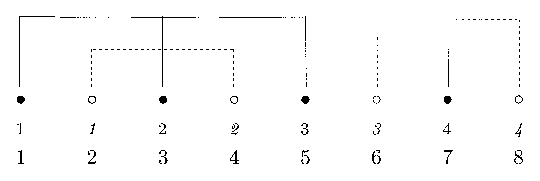
\includegraphics{chap02-vend-scan-02.eps}
\end{figure}

\noindent where $\alpha,\,\alpha^{\prime}$ are the fixed points of
an elliptic substitution $E$ of period $l$:
\begin{equation*}
z^{\prime}=Ez,\qquad \frac{z^{\prime}-\alpha}{z^{\prime}-\alpha^{\prime}}=\varepsilon\,\frac{z-\alpha}{z-\alpha^{\prime}},\qquad \varepsilon=e(1/l).
\end{equation*}
Let $K$ be a fixed circle of $E$ that contains $\alpha$ but not $\alpha^{\prime}$, as shown in the Figure. If $\lambda_{1}$ is an arc of a circle through $\alpha$ and $\alpha^{\prime}$ orthogonal to $K,\,E$ maps it into a similar arc $\lambda_{2}$ making an angle of $2\pi/l$ with $\lambda_{1}$. Continued application results in $l$ arcs $\lambda_{1},\,\cdots,\,\lambda_{l}$, each making an angle of $2\pi/l$ with its predecessor.

Write $w=\zeta^{l};\zeta =(z-\alpha)/(z-\alpha^{\prime})$ is a linear transformation mapping $\lambda_{i}$ into a straight line $\lambda_{i}^{\prime}$ through the origin, for $\lambda_{i}$ goes through $\alpha^{\prime}$. Because of the conformality, the lines $\lambda_{1}^{\prime},\,\cdots,\,\lambda^{\prime}_{l}$ are equally spaced around the circle. Since $K$ is orthogonal to all $\lambda_{i},\,\zeta(K)$ is orthogonal to all $\lambda_{i}^{\prime}$ and is therefore a circle about the origin. Thus $\zeta$ maps the curvilinear sector bounded by $\lambda_{i},\lambda_{i+1}$
into a straight-sided sector bounded by $\lambda_{i}^{\prime},\lambda_{i+1}^{\prime}$.

We see now that the function $w$ of \eqref{ch02:eqn14} maps the interior of $K$ onto the interior of a disk $D$ about the origin in an $l$ to 1 manner.
The inverse image of a point of $D$ other than 0 consists of $l$ distinct points in $K$ that are images of each other by powers of $E$, while 0 corresponds only to $\alpha$. The function $w$ is regular in $K$.

Finally we discuss the mapping
\begin{equation}\label{ch02:eqn15}
w= e(l/c(z-p)).
\end{equation}
\begin{figure}[!h]
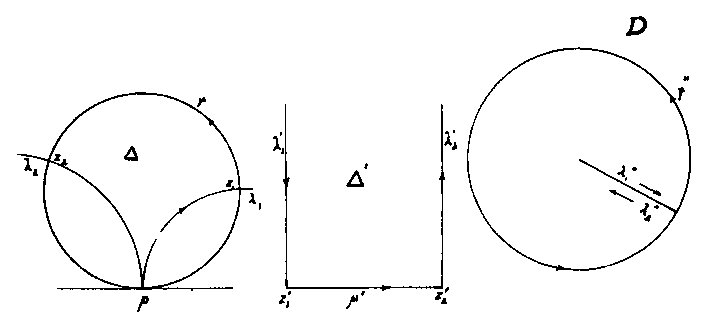
\includegraphics{chap02-vend-scan-03.eps}
\end{figure}

\noindent where $p$ is the fixed point of the parabolic
transformation
\begin{equation*}
z^{\prime}=Pz,\qquad \frac{1}{z^{\prime}-p}=\frac{1}{z-p}+c,\qquad c,\,\neq
0.
\end{equation*}
Let $K$ be a fixed circle $P$. We consider the triangular region $\Delta$ bounded by two circular arcs $\lambda_{1}$ and $\lambda_{2} = P\lambda_{1}$ passing through $p$ and orthogonal to $K$ and by an arc $\mu$ of $K$ (cf. Figure). $\Delta$ includes $\lambda_{1}$ and $\lambda_{2}$ but not $\mu$.

We consider $w$ as a composition: $w = \tau \circ\zeta$ where $\zeta= 1/c(z-p), \tau = e(\zeta)$. The function $\zeta$ is a linear transformation mapping $\Delta$ into $\Delta^{\prime}$, a partly closed
region bounded by two parallel lines $\lambda_{1}^{\prime},\lambda_{2}^{\prime}$ and a segment $\mu^{\prime}$ perpendicular to them. The point $p$ goes to $\infty$. Since $z_{2} = Pz_{1}$, we have $z_{2}^{\prime} =1/c(z_{2} - p) = 1/c(z_{1} - p) + 1 = z_{1}^{\prime} + 1$. Thus $\mu^{\prime}$ is horizontal.

Next, we apply the second mapping $\tau = e(\zeta)$. The region $\Delta^{\prime}$ is carried into the interior of a disk $D,\lambda_{1}^{\prime}$ and $\lambda_{2}^{\prime}$ becoming coincident radii because of
$\lambda_{2}^{\prime} = \lambda_{1}^{\prime} + 1$. The radius of $D$ is $\exp\, (-2\pi\ {\rm Im}\, \mu^{\prime})$. The point $\infty$ goes into the origin.

It is now seen that the composite function $w = \tau\circ\zeta$ of \eqref{ch02:eqn15} maps $\Delta$ onto $D$, the point $p$ going to 0 and a curve in $\Delta$
ending at $p$ going into a curve in $D$ ending at 0. The mapping is 1-1 except for points on $\lambda_{1}$ and $\lambda_{2}$ that correspond under $P$; these are carried to the same point in $D$.

We discuss the mappings of the disk $K$ under \eqref{ch02:eqn15}. $K$ is made up of $\Delta$ and its images under the powers of $P$:
\begin{equation*}
K=\bigcup_{m=1}^{\infty}P^{m}\Delta.
\end{equation*}
The function $w$ then maps the interior of $K$ onto $D$, infinitely many points of $K$ going into a single point of $D$. The inverse image of a point of $D$ other than 0 consists of a point in $K$ and all its images under powers of $P;$ 0 corresponds only to $p$.

The function $w$ is regular in the interior of $K$. Moreover $w$ is continuous at $p$ on approach within $K$. Indeed, let $\omega_{n}$ be a sequence of points in $K$ tending to $p$. Each $\omega_{n}$ is equivalent under a power of $P$ to a point $\omega_{n}^{\prime}$ in $\Delta$. Hence $w(\omega_{n})=w(\omega_{n}^{\prime})\rightarrow 0$, which establishes our assertion.

\textsc{References} : \citeauthor{Caratheodory0000}~[\ref{Caratheodory3}];\index{Carath\'{e}odory} \citeauthor{Ford0000}~[\ref{Ford1}]\index{Ford}, Chs. 1, VIII; \citeauthor{Titchmarsh0000}~[\ref{Titchmarsh1}]\index{Titchmarsh}, Ch. VI.


\section{Linear Transformations}\label{ch02:sec9}\index{linear transformation}

\subsection{}\label{ch02:sec9A}
Throughout the book we shall assume that all linear transformations have determinant 1. (This can always be secured by dividing each coefficient by $(ad -bc)^{1/2}$, which we have assumed to be different from zero.) \emph{That is, the term} ``\emph{linear transformation}'' \emph{shall mean a function of the form}
\begin{equation*}
z^{\prime}=Tz=\frac{az+b}{cz+d},\qquad ad\,-bc=1.
\end{equation*}
A linear transformation is therefore nonsingular.

We list the major well-known properties of linear transformations.

1) A linear transformation maps the complex sphere $\mathscr{Z}$ on itself in a 1-1 directly conformal manner. In particular, a linear transformation is a homeomorphism.

2) A linear transformation preserves the family consisting of all circles and straight lines.

3) A linear transformation preserves the cross-ratio of 4 points.

4) Given two triples $(z_{1},\,z_{2},\,z_{3}),\,(w_{1},\,w_{2},\, w_{3})$ such that the $\{z_{i}\}$ are distinct points and the $\{w_{i}\}$ are distinct points, there is one and only one linear transformation $T$ such that $Tz_{i}=w_{i},\,i=1, 2,3$.

5) If $p$ and $q$ are inverse points with respect to a circle $C$ and $T$ is a linear transformation, then $T(p)$ and $T(q)$ are inverse points with respect to the circle (or straight line) $T(C)$.


\subsection{}\label{ch02:sec9B}
If $S$ and $T$ are linear transformations\index{linear transformation!transforms of a}, the composition or product $ST$
is defined to he the function $S(T(z))$; it is defined everywhere. Thus in this book products are read from right to left. One verifies immediately that $ST$ is also a linear transformation. Since $S$ is 1-1, $S^{-1}$ exists, is defined everywhere, and is likewise a linear transformation. The associative law $S(TU)=(ST)U$ is evident, is evident, and the transformation $I$, defined by $Iz = z$ for all $z$, serves as an identity. \emph{The set of all linear transformations forms a group under the above multiplication}\index{linear transformation!group of\_\_\_s}.

The product $STS^{-1}$ is called a \emph{transform} of $T$. If $A$ is a set and $T$ maps $A$ on $B$, then $STS^{-1}$ maps $S(A)$ on $S(B)$. The transition from $T$ to $STS^{-1}$ amounts merely to a change of coordinates in the plane.


\subsection{}\label{ch02:sec9C}
If $T\neq I$ is a linear transformation, $T$ has one or two fixed\index{linear transformation!fixed circle of} points\index{linear transformation!fixed points of}. In the first case $T$ is called \emph{parabolic}\index{linear transformation!parabolic}.

Let $T$ be parabolic with fixed point $z_{0} \neq\infty$ and let $S$ be a
linear transformation sending $z_{0}$ to $\infty$, for example, $Sz=-1/(z-z_{0})$. Let $T^{\prime}= STS^{-1} =(a^{\prime}z+b^{\prime})/(c^{\prime}z+d^{\prime})$.
$T^{\prime}$ is unimodular and has the unique fixed
point $\infty$, hence is of the form
{\def\theequation{16a}
\begin{equation}\label{ch02:eqn16a}
T^{\prime}z=(a^{\prime}z+b^{\prime})/d^{\prime}=z\pm b^{\prime}.
\end{equation}}
(Note $a^{\prime}d^{\prime}=1$, and $a^{\prime}/d^{\prime}=a^{\prime2}=1$ since $T^{\prime}$ has no finite fixed point.)

When $T$ has two distinct fixed points, we select an $S$ which carries these points to 0 and $\infty$; then $T^{\prime}=STS^{-1}$ has fixed points 0 and $\infty$ and is of the form
{\def\theequation{16b}
\begin{equation}\label{ch02:eqn16b}
T^{\prime}z=\frac{a^{\prime}z}{d^{\prime}}=\kappa^{\prime}z.
\end{equation}}
Here $\kappa^{\prime}=\kappa(T^{\prime})$, called multiplier of $T^{\prime}$, is any complex number except 0 or 1. Write $\kappa^{\prime}=\rho e^{i\theta},\,\rho >0,\,0\leqq\theta<2\pi$. If

$\rho =1,\quad \theta\neq0,\quad T^{\prime}$ is called \emph{elliptic}\index{linear transformation!elliptic},

$\rho \neq 1,\quad\theta=0,\quad T^{\prime}$ is called \emph{hyperbolic}\index{linear transformation!hyperbolic},

$\rho \neq 1,\quad \theta\neq0,\quad T^{\prime}$ is called \emph{loxodromic}\index{linear transformation!loxodromic}.

Denote by $\chi(T^{\prime})=\chi^{\prime}$ the \emph{trace}\index{linear transformation!trace of} $a^{\prime}+d^{\prime}$ of the transformation $T^{\prime}$. Both trace and multiplier are invariant under $T\rightarrow STS^{-1}$. \emph{Hence} $T$ \emph{and} $T^{\prime}$ \emph{are} \emph{simultaneously elliptic, parabolic, hyperbolic, or loxodromic}.

Going back to the transformation $T$, we have the \emph{normal forms} $(z^{\prime}= Tz)$:
\begin{subequations}
\begin{gather}\label{ch02:eqn17a}
\frac{1}{z^{\prime}-\xi}=-\frac{1}{z-\xi}+c,\quad \mbox{ parabolic, fixed point}\ \xi,\\
\label{ch02:eqn17b} \frac{z^{\prime}-\xi_{1}}{z^{\prime}-\xi_{2}}=\kappa\,\frac{z-\xi_{1}}{z-\xi_{2}},\qquad \mbox{nonparabolic, fixed point}\ \xi_{1},\,\xi_{2}.
\end{gather}
\end{subequations}

Trace and multiplier of $T$ satisfy the equations
\begin{equation}\label{ch02:eqn18}
\kappa +\kappa^{-1}=\chi^{2}-2,\qquad \kappa^{1/2} +\kappa^{-1/2}=\chi.
\end{equation}
These relations also hold for parabolic $T$ if we define $\kappa = 1$. Then we read off the following: \emph{Necessary and sufficient that} $T$ \emph{be elliptic,parabolic, or hyperbolic is that} $\chi$ \emph{be real and} $|\chi|<2,\,|\chi|=2$, or $|\chi|>2$, \emph{respectively. Necessary and sufficient that} $T$ \emph{be loxodromic is that} $\chi$ \emph{be nonreal}.

Certain substitutions are of \emph{finite order} or \emph{periodic}\index{linear transformation!parabolic}, i.e., $T^{n}=I$ for an integer $n$. Obviously this happens if and only if $\kappa^{n}=1$, i.e., if and only if $\kappa$ is a root of unity $e(\theta),\,\theta=p/q$, rational. Then $T$ is elliptic. The \emph{only transformations of finite order are certain of the elliptic ones}. Note that in this case $\chi=2 \cos \pi p/q$.


\subsection{}\label{ch02:sec9D}
By a \emph{fixed circle} or \emph{fixed line} of a transformation $T$ we mean one which is mapped on itself by $T$. The fixed circles and lines of a transformation $T^{\prime}$ of the form (16) are easily determined. Then going back to $T$ by the substitutions $S^{-1}$, we find the following well-known facts.

1) If $T$ is parabolic, there is a line through the fixed point such that each fixed circle of $T$ is tangent to this line at the fixed point, and conversely, each circle tangent to this line at the fixed point is a fixed circle of $T$. $T$ preserves the interior of each fixed circle. There is a second family of mutually tangent circles orthogonal to the family of fixed circles; this family is mapped on itself by $T$.

2) If $T$ is hyperbolic, each circle through the fixed points is a fixed circle, and conversely. $T$ preserves the interior of every fixed circle. The family of circles orthogonal to the family of fixed circles is mapped on itself by $T$.

3) If $T$ is elliptic, each circle through the fixed points is mapped by $T$ onto another circle through the fixed points. The family of circles orthogonal to the above family is the family of fixed circles. $T$ preserves the interior of a fixed circle.

4) If $T$ is loxodromic, there are no fixed circles unless the multiplier $\kappa$ is real and negative. In the latter case a circle through the fixed points is a fixed circle, but $T$ maps its interior on its exterior. \emph{A loxodromic transformation never preserves the interior of a circle}.


\subsection{}\label{ch02:sec9E}
A linear transformation $T$ that maps the upper half-plane. $\mathscr{H}$ on itself has real coefficients, and conversely.


\begin{proof*}
Suppose $c\neq 0$. $T(\infty)=a/c,\,T^{-1}(\infty)=-d/c$, and $T(0)=b/d$ are all real. Hence $Tz=(ac^{-1}z+bc^{-1})\cdot(z+dc^{-1})^{-1}$ has real coefficients and real determinant $D=(ad-bc)c^{-2}=c^{-2}$. Now $D<0$ would imply $T$ maps $\mathscr{H}$ on the lower half-plane, since
\begin{equation*}
{\rm Im}\ Tz=D\cdot{\rm Im}\ z\cdot|z+dc^{-1}|^{-2}.
\end{equation*}
Hence $D>0$, i.e., $c$ is real. It follows that $a,\,b,\,d$ are real. If $c=0$, a similar construction, using $T^{-1}(0)=-b/a$, is effective. This proves the direct part of the theorem. The converse is obvious.

Let $T$ be a linear transformation with real coefficients. Then \ref{ch02:sec9D}
shows the following (the fixed circle here is the real axis): If $T$ is parabolic or hyperbolic, each fixed point is real. If $T$ is elliptic, the fixed points are complex conjugate nonreal numbers. $T$ is never loxodromic.

A linear transformation $V$ which maps the unit disk $\mathscr{U}:|z| < 1$ on itself has the form
\begin{equation*}
V z=\frac{az+\overline{c}}{cz+\overline{a}}\qquad a\overline{a}-c\overline{c}=1.
\end{equation*}
Let $\mathscr{Q}$ be the boundary of $\mathscr{U}$. When $V$ is parabolic or hyperbolic, each fixed point lies on $\mathscr{Q}$. When $V$ is elliptic, its fixed points are inverse with respect to $\mathscr{Q}$ and do not lie on $\mathscr{Q}$. $V$ is never loxodromic.

It is clear that $T$ and $V$ each depend on 3 real parameters.
\end{proof*}

\subsection{}\label{ch02:sec9F}
\setcounter{theorem}{0}
\begin{theorem}\label{ch02:thm1a} Two linear transformations, with the same set of fixed points are commutative\index{linear transformation!commutative\_\_\_s} provided neither is the identity.
\end{theorem}


\begin{proof*}
Suppose $V_{1},\,V_{2}$ are parabolic substitutions. Let $A$ be chosen so that $V_{1}^{\prime}=A V_{1}A^{-1},\,V_{2}^{\prime}=A V_{2}A^{-1}$ have the unique fixed point $\infty$. Then $V_{1}^{\prime}z=z+\lambda_{1},\,V_{2}^{\prime}z=z+\lambda_{2}$ and obviously $V_{1}^{\prime}$ commutes with $V_{2}^{\prime}$. Hence $V_{1}$ commutes with $V_{2}$. Secondly, suppose $V_{1},V_{2}$ have a common pair of fixed points; choose $A$ so that $V_{i}^{\prime}=\alpha_{i}z,\ \alpha_{i}\neq0,1$, and the result is again obvious.\:\:\:q.e.d.
\end{proof*}

In future proofs of this type we shall not mention the transformation $A$
explicitly but say instead: we may assume (without loss of generality) that
$V_{1}$ has its fixed point at $\infty$, etc.

\begin{theorem}\label{ch02:thm2a}
 two linear transformations are commutative, neither being
the identity, either both have the same set of fixed points or both are substitutions
of period two \emph{(}and so elliptic\emph{)}.
\end{theorem}

\begin{proof*}
Suppose $V_{1}$ is parabolic with fixed point at $\infty$;  write $V_{1}z= z+\lambda,\,V_{2}z=(az+b)/(cz+d),\,ad -bc=1$. $V_{1}$ and $V_{2}$ commute if and only if the commutator $C=V_{1} V_{2}V_{1}^{-1}V_{2}^{-1}=I$. By calculation
\begin{equation*}
Cz=\frac{(1+ac\lambda+c^{2}\lambda^{2})z+\lambda-a^{2}\lambda-ac\lambda^{2}}{c^{2}\lambda z+1-ac\lambda},
\end{equation*}
which shows that $C=I$ only if $c=0$ and $\lambda(1-a^{2}-ac\lambda) =0$. Since $\lambda\neq0$, the second condition gives $a^{2}=1, a=\pm 1$. From $ad -bc=1$ and $c=0$ we now deduce $d=\pm\, 1$. Hence $a+d=\pm\,2$ and $V_{2}$
is parabolic with fixed point $\infty$.

If $V_{1}$ has fixed points 0 and $\infty$ and $V_{2}$ is as before, we compute, since $V_{1}z=\alpha z,\,\alpha\neq 0,1$,
\begin{equation*}
Cz=\alpha\,\frac{(ad-bc\alpha)z+ab(\alpha-1)}{cd(1-\alpha)z+(-bc+ad\alpha)}.
\end{equation*}
Since $\alpha\neq 0,1$, we get, on setting $C=I$, that $ab=cd=0$. Now if $bc=0$, then from $ad-bc =1$ we conclude $ad\neq 0$ and $a\neq 0,\,d\neq 0$. Then $b=c =0$ and $V_{2}$ has fixed points $0$ and $\infty$. In the opposite case $(bc\neq 0)$ we find $a=d=0$. Then $ad -bc=1$ implies $bc=-1$, so that $V_{2}z= b/cz=-b^{2}/z$ and $V_{2}$ has period two. Moreover $C=I$ yields $\alpha(ad-bc\alpha) = -bc+ad\alpha$, which reduces to $\alpha^{2}=1$ or $\alpha=-1$. Hence $V_{1}z$ is also of period two.
\end{proof*}

\subsection{}\label{ch02:sec9G}
By the same method we can compute the commutator of\index{linear transformation!commutator of\_\_\_s} various transformations and so obtain:

1) If $U,\,V$ are nonparabolic with $\infty$ as a common fixed point and the second fixed points distinct, then $U VU^{-1}V^{-1}$ is parabolic with fixed point $\infty$ and is not the identity.

2) If $U,\,V$ are parabolic with different fixed points, then either $UV$ is loxodromic or if not, $U VU^{-1}V^{-1}$ is hyperbolic.


\subsection{}\label{ch02:sec9H}
The limit of\index{linear transformation!limit of\_\_\_s} a sequence of linear transformations is a function of very simple behavior (cf. \citeauthor{Piranian0000}\index{Piranian-Thron} [\ref{Piranian}]).
\begin{theorem*}
Let $(T_{n}(z))$ be a sequence of linear transformations and define
\begin{equation*}
f(z)=\lim_{n\rightarrow\infty}T_{n}(z)
\end{equation*}
for each $z$ for which the sequence converges. If the range of $f$ contains $3$ distinct values, $f$ is a linear transformation; the convergence is then valid everywhere and is uniform on compact sets which avoid the pole of $f$. Moreover, for suitable $\varepsilon_{2}=\pm 1$, we have $\varepsilon_{n}T_{n}\rightarrow f$, where $T_{n},\,f$ are the matrices associated with $T_{n}z,\,f(z)$, respectively. Finally, if $(T_{n}z)$ converges uniformly in a closed region, $f(z)$ is either constant or a linear transformation and in the latter case $\varepsilon_{n}T_{n}\rightarrow f$.
\end{theorem*}


\begin{proof*}
The function $f$ is single-valued wherever it is defined. Let $f(z_{i})=w_{i},\,i=1,2,3$, the $\{w_{i}\}$ being distinct. Since the $\{z_{i}\}$ are obviously distinct, we can determine two linear transformations $Z$ and $W$ such that $Z(0)=z_{1},\,Z(1)=z_{2},\, Z(\infty)=z_{3}$ and $W(w_{1})=\infty,\, W(w_{2})=-1,\,W(w_{3})=0$. Define $WT_{n}Z=X_{n}$. Then $X_{n}(0)\rightarrow\infty,\, X_{n}(\infty)\rightarrow 0,\,X_{n}(1) \rightarrow-1$.

Let $X_{n}=(a_{n}\,b_{n}\,|\,c_{n}d_{n})$. The above limits give \eqref{ch02:eqn1} $a_{n}/c_{n}\rightarrow 0$, \eqref{ch02:eqn2} $(a_{n}+b_{n})/(c_{n}+d_{n})\rightarrow-1$. Since
\begin{equation*}
X_{n}z=\frac{a_{n}}{c_{n}}-\frac{1}{c_{n}^{2}}\frac{1}{z+d_{n}/c_{n}},
\end{equation*}
we get from $X_{n}(0)\rightarrow\infty$ the relation \eqref{ch02:eqn3} $c_{n}d_{n}\rightarrow 0$, and from $X_{n}(1)\rightarrow-1$ we get $c_{n}(c_{n}+d_{n})\rightarrow 1$. Therefore $c_{n}^{2}\rightarrow 1$. Hence, for a suitable sequence $\varepsilon_{n}=\pm 1$, we can have $\varepsilon_{n}c_{n}\rightarrow 1$. It follows from \eqref{ch02:eqn1} and \eqref{ch02:eqn3} that $a_{n}\rightarrow 0,\,d_{n}\rightarrow 0$, and $\varepsilon_{n}b_{n}=(\varepsilon_{n}a_{n}\cdot\varepsilon_{n}d_{n}-1)/\varepsilon_{n}c_{n}\rightarrow-1$. Thus $\varepsilon_{n}X_{n}\rightarrow X =(0-1|1\,0)$ and $\varepsilon_{n}T_{n}=W^{-1}\cdot\varepsilon_{n}X_{n}\cdot Z^{-1}\rightarrow W^{-1}XZ^{-1}$.

This implies that $T_{n}(z)\rightarrow W^{-1}XZ^{-1}(z)=f(z)$ for each $z$; hence $f(z)$ is a linear transformation and the convergence is valid for all $z$. On a compact set $S$ which avoids the pole of $f$ it is seen that the family $\{T_{n}(z)\}$ is uniformly bounded and by Vitali's theorem (\ref{ch02:sec7F}) the convergence of $T_{n}z$ is uniform on $S$.

The final conclusion of the theorem is proved in the following way. Since $T_{n}$ is univalent in a closed region $D$ and the convergence is uniform in $D,\,f(z)$ is either constant or univalent in $D$ (cf.~\ref{ch02:sec8B}). If $f(z)$ is univalent it assumes infinitely many distinct values. Hence by what we have already proved $f(z)$ is a linear transformation and $\varepsilon_{n}T_{n}\rightarrow f$.
\end{proof*}

\subsection{}\label{ch02:sec9I}
The following special result will be required.

\begin{theorem*}
If $K$ is a disk and if $V(K)$ is a proper subset of $K$, then $V$ is hyperbolic or loxodromic and $V(K)$ contains a fixed point of $V$.
\end{theorem*}


\begin{proof*}
Assume $V$ normalized so that $V$ is either $V_{1}=\kappa z$ or $V_{2}=z+\lambda,\,\kappa \neq0,\,1,\,\lambda\neq 0$. Clearly $V_{2}(K)$ is disjoint from $K$ or overlaps it. When $V_{1}$ is elliptic, it rotates $K$ about the origin, so $V_{1}(K)$ cannot be properly contained in $K$.

Hence $V$ is hyperbolic or loxodromic with fixed points $0$ and $\infty$. If $V(K)$ does not enclose the origin, the same must be true of $K$. Let $|K|M$ and $|K|m>0$ he the maximum and minimum distances from the origin to $V(K)$, where $|K|$ is the diameter of $K$. Then the analogous quantities for $K$ must be $M$ and $m$. Since $V(K)$ is contained in $K$, we now have $m<|K|m<|K|M<M$, a contradiction.
\end{proof*}

\textsc{References}:
\citeauthor{Caratheodory0000}\index{Carath\'{e}odory} [\ref{Caratheodory1}], Ch. \ref{ch02:chap02}; \citeauthor{Ford0000}~[\ref{Ford1}]\index{Ford}, Chs. I, \ref{ch02:chap02}.

\skiptoctrue
\section*{Exercises}

1. If $U$ and $V$ are nonloxodromic and of the same class (i.e., elliptic, parabolic, etc.) and both fix $\infty$, then $UV$ and $VU$ are of that class and fix $\infty$. If $U,\,V$ are loxodromic and fix $\infty$, then $UV,VU$ are either both loxodromic or both hyperbolic and fix $\infty$.

2. If $U$ is elliptic, $V$ parabolic, and both fix $\infty$, then $UV$ and $VU$ are elliptic and fix\index{linear transformation!fixed points of} $\infty$.

3. Let $T$ be nonelliptic. If for any $z,\,T^{n_{j}}z\rightarrow z_{0},\, n_{j}\rightarrow\infty$, then $z_{0}$ is a fixed point of $T$. The result is not true for elliptic $T$.

4. For linear transformations\index{linear transformation!commutative\_\_\_s} that preserve the interior of the unit disk, the exact converse of~\ref{ch02:sec9F}, Theorem~\ref{ch02:thm1a} is true.

\section{The Isometric Circle}\label{ch02:sec10}\index{isometric circle}

\subsection{}\label{ch02:sec10A}
\begin{definition*} Let $Tz=(az\,+b)/(cz+d)$ be a linear transformation which does not fix $\infty$ (i.e., $c\neq 0$). The isometric circle of $T$, denoted by $\mathfrak{J}(T)$, is the circle
\begin{equation*}
\Im(T):|cz+d|=1.
\end{equation*}
Since $T^{\prime}(z)=(ad-bc)(cz+d)^{-2}=(cz\,+d)^{-2}$, we see that $\Im(T)$ is the locus of points $z$ such that a line element at $z$ is unaltered in length by the mapping $T$. If $T$ is considered as a matrix, we have $\mathfrak{J}(T)=\Im(-T)$. We do not define an isometric circle for a transformation fixing $\infty$.
\end{definition*}

\begin{theorem*}
$T$ maps $\Im(T)$ on $\Im(T^{-1})$ and maps the interior \emph{(}exterior\emph{)} of $\Im(T)$ on the exterior \emph{(}interior\emph{)} of $\Im(T^{-1})$.
\end{theorem*}

For if $z \in\Im(T)$, we have
\begin{equation*}
|cTz-a|^{-2}=\bigg|c\frac{az+b}{cz+d}-a\bigg|^{-2}=\bigg|\frac{1}{cz+d}\bigg|^{-2}=1;
\end{equation*}
hence $Tz\in\Im(T^{-1})$. If $z\in \mathrm{Int}\,\Im(T)$, then $|cz+d|<1$, and so $|cTz -a|^{-2}>1$; hence $Tz\in \mathrm{Ext}\,\Im(T^{-1})$, etc.


\subsection{}\label{ch02:sec10B}
We now consider isometric circles of powers of $T$. Suppose $T$ is parabolic with finite fixed point---cf. (\ref{ch02:eqn17a}). By iteration we obtain $(T^{n}z-\xi)^{-1}=(z-\xi)^{-1}+nc$, or
\begin{equation*}
T^{n}z=\frac{(1+nc\xi)z-nc\xi^{2}}{ncz+1-nc\xi},
\end{equation*}
and this is a linear transformation since its determinant equals 1. Hence
\begin{equation*}
\Im(T^{n}):\bigg|z-\bigg(\xi-\frac{1}{nc}\bigg)\bigg|=\frac{1}{|nc|}.
\end{equation*}
All isometric circles are tangent at $\xi$. The circles with $n>0$ lie within $\Im(T)$; those with $n< 0$ lie within $\Im(T^{-1})$.

When $T$ has two finite points we obtain in the same way from (\ref{ch02:eqn17b});
\begin{equation*}
T^{n}z=\frac{(\kappa^{n}\xi_{2}-\xi_{1})z+(1-\kappa^{n})\xi_{1}\xi_{2}}{(\kappa^{n}-1)z+\xi_{2}-\kappa^{n}\xi_{1}},
\end{equation*}
where the determinant is $\kappa^{n}(\xi_{1}-\xi_{2})^{2}$. Normalize by dividing by $\kappa^{n/2}(\xi_{1}-\xi_{2})$ and obtain
\begin{equation*}
\tag{$^\ast$} \Im(T^{n}):\bigg|z -\frac{\kappa^{n/2}\xi_{1}-\kappa^{-n/2}\xi_{2}}{\kappa^{n/2}-\kappa^{-n/2}}\bigg|=\bigg|\frac{\xi_{1}-\xi_{2}}{\kappa^{n/2}-\kappa^{-n/2}}\bigg|.
\end{equation*}

Let $T$ be elliptic; $|\kappa|=1$. The above equation becomes an identity for $z=\xi_{1},\,\xi_{2}$; hence all isometric circles $\Im(T^{n})$ pass through the fixed points. When $T$ is periodic there are only a finite number of different isometric circles. The Figure on page 76 illustrates the case of period 4.

For the discussion of the hyperbolic case we shall need a lemma.

\begin{lemma*} If $\Im(T)$ is exterior to $\Im(T^{-1})$, then $\mathfrak{J}(T^{2})$ is interior to $\mathfrak{J}(T)$.
\end{lemma*}


\begin{proof*}
Let $z$ be on or outside $\Im(T)$. Then $|cz+d|\geqq 1$. Also $Tz$ is on or inside $\mathfrak{J}(T^{-1})$ and so outside $\Im(T)$. Hence $|cTz+d|>1$. Let $T^{2}z=(\alpha z+\beta)/(\gamma z+\delta)$. From the easily verified identity,
\begin{equation*}
\gamma z+\delta=(cTz+d)(cz+d),
\end{equation*}
we conclude that $|\gamma z +\delta|>1$, i.e., $z$ is outside $\Im(T^{2})$. Every point on or outside $\Im(T)$ is outside $\mathfrak{J}(T^{2})$, whence $\Im(T^{2})$ is inside $\Im(T)$.\:\:\:q.e.d.

Let $T$ be hyperbolic; $\kappa >0,\,\kappa \neq 1$. The isometric circles $\mathfrak{J}(T),\,\mathfrak{J}(T^{-1})$ are exterior to each other, for the distance between their centers, $|(a+d)/c|$, is greater than $2/|c|$, the sum of their radii. Hence, be the lemma, $\Im(T^{2})$ is within $\mathfrak{J}(T)$ and likewise $\Im(T^{-2})$ is within $\Im(T^{-1})$. By induction one establishes easily that $\Im(T^{n})$ is within $\Im(T^{n-1})$ all $\Im(T^{-n})$ is within

\begin{figure}[!h]
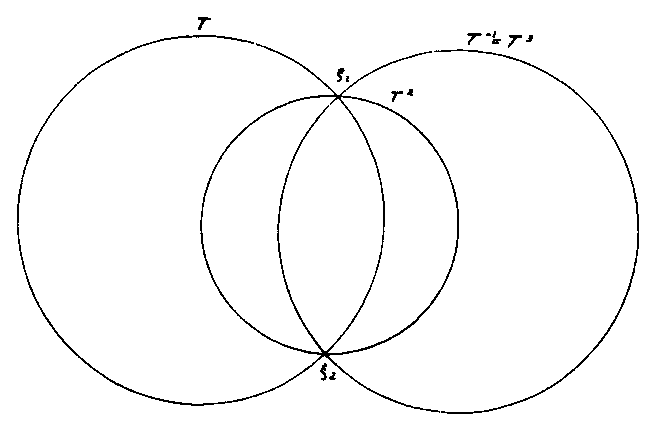
\includegraphics{chap02-vend-scan-04.eps}
\end{figure}

\noindent $\Im(T^{-n+1})$ for $n=1,\, 2,\cdots$. Moreover, the substitution $z=\xi_{1}$ makes the left member of $(^\ast)$ less than the right member when $n>0$ and $\kappa >1$, and $z=\xi_{2}$ has the same effect in the equation obtained by replacing $n$ by $-n$ (the equation for $\Im(T^{-n})$). The same results hold, \emph{mutatis mutandis}, when $\kappa <1$. Hence, one fixed point of $T$ lies within all $\Im(T^{n})$ for $n>0$; the other fixed point lies within all $\Im(T^{n})$ with $n<0$.
\end{proof*}

\subsection{}\label{ch02:sec10C}
\begin{theorem*} If $T$ is a linear transformation having a fixed circle $\mathscr{C},$ then $\Im(T)$ is orthogonal to $\mathscr{C}$.
\end{theorem*}

We consider only the cases in which $\mathscr{C}$ is the real axis or the unit circle $\mathscr{Q}$. The first case is obvious, for $T$ has real coefficients (\ref{ch02:sec9E}), so the center of $\Im(T)$ is real. In the second case $T=(a\,\bar{c}|c\,\bar{a}),a\bar{a}- c\bar{c}=1.$ $\Im(T)$ will be orthogonal to $\mathscr{Q}$ provided $1=OD^{2}=OA\cdot OC$. (Cf. Figure.) Now $OB= |-\bar{a,}/c|,\,AB=BC=1/|c|$. Hence
\begin{equation*}
OA \cdot OC =\frac{|a|-1}{|c|}\cdot \frac{|a|+1}{|c|} =1  \qquad \mathrm{q.e.d}.
\end{equation*}

\textsc{Reference}: \citeauthor{Ford0000}~[\ref{Ford1}]\index{Ford}. Ch.~\ref{ch01:chap01}.

\begin{figure}[!h]
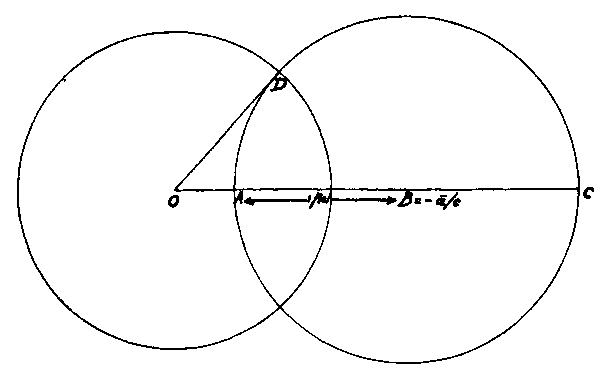
\includegraphics{chap02-vend-scan-05.eps}
\end{figure}


\skiptoctrue
\section*{Exercise}

1. If $\Im(T),\,\Im(T^{-1})$ are tangent externally, $\Im(T^{2})$ is tangent internally to $\Im(T)$.

\section{Groups of Linear Transformations}\label{ch02:sec11}

\subsection{}\label{ch02:sec11A}
We shall sometimes denote the linear transformation $Tz=(az+b)/(cz+d)$ by $\overline{T}$ or $\overline{T}z$. \emph{The} $2\times2$ \emph{matrix}
\begin{equation*}
T=\left(\begin{matrix}
a & b\\c & d
\end{matrix}\right),\qquad ad-bc=1
\end{equation*}
\emph{will be written} $(a\,b|c\,d)$. The matrix $(\rho a,\,\rho b\,|\rho c,\,\rho d)$ will be denoted by $\rho T,\,\rho =$ complex number.

Let $\bar{\Omega}$ be the group of all $\overline{T}$ (cf.~\ref{ch02:sec9B}) and $\Omega$ the group of all $T$ (cf.~\ref{ch02:sec5D}). $\Omega$ and $\bar{\Omega}$ are homomorphic under the mapping $\rho T \rightarrow\overline{T},\,\rho \neq 0.$ The kernel of the homomorphism is $\{\rho I)$; thus $\Omega/\{\rho I\}$ is isomorphic with $\bar{\Omega}$.

In the present case $\rho =\pm 1$, since the determinant of $\rho T$ is 1. The quotient group becomes $\Omega/\{I,\,-I\}$; i.e., it identifies $T$ and $-T$ in $\Omega$.

In this book we shall be concerned with subgroups of both $\Omega$ and $\bar{\Omega}$. Usually it makes no difference whether we consider the subgroup of linear transformations or the subgroup of matrices. We shall make a distinction only when it is important to do so.

Let $G$ be a subgroup of $\Omega$. If $G$ does not contain $-I$, we can adjoin this element; that is, we can consider a new group $G^{\ast}$ such that $G^{\ast}/\{I,\,-I\}=G$. Both $G$ and $G^{\ast}$ are associated with the same group $\bar{G}$ of linear transformations. Whenever convenient, then, we may assume a group of matrices contains $-I$.


\subsection{}\label{ch02:sec11B}
Let $G$ be a group of linear transformations and let $A$ be a subset of the complex sphere. The set of elements $T\in G$ such that $TA=A$ is a subgroup of $G$. It is denoted by $G_{A}$ and is called the \emph{isotropy subgroup} of $A$. The most important case for us occurs when $A$ is a single point $p$. Then $G_{p}$\index{$G_{p}$} consists of those elements of $G$ for which $p$ is a fixed point. We shall use this notation systematically.


\subsection{}\label{ch02:sec11C}
Let $p$ be a fixed point of $T\in G$ and let $A\in G$. Then $A(p)$ is a fixed point of $ATA^{-1}$. We have $G_{Ap}=AG_{p}A^{-1}$. The group $AG_{p}A^{-1}$ is said to be \emph{conjugate}\index{conjugate group ( = transformed group)} to $G_{p}$. The collection of all subgroups of $G$ conjugate to $G_{p}$ is called the \emph{conjugacy class}\index{conjugacy class} of $G_{p}$. The conjugacy class of $G_{p}$ consists of all the elements of $G$ which fix a point of the set $G_{p}$. (Recall that $Gp$ is the set $\{T(p)|T\in G\}.)$


\subsection{}\label{ch02:sec11D}
We have defined the convergence\index{convergence of group elements} of a sequence of matrices in 6B. Let $T_{n}=(a_{n}\,b_{n}|c_{n}\,d_{n}),\,T= (a\,b|c\,d)$. If $T_{n}\rightarrow T$, \emph{then} $\overline{T}_{n}z\rightarrow\overline{T}z$ \emph{for each} $z\in \mathscr{Z}$.


\begin{proof*}
Suppose $z$ finite and $cz +d\neq0$. Then $c_{n}z+d_{n}\neq 0$ for $n>N$ and
\begin{align*}
\overline{T}_{n}z-\overline{T}z=(c_{n}z+d_{n})^{-1}(cz+d)^{-1}\{&(a_{n}c-ac_{n})z^{2}+\\
&(a_{n}d-ad_{n}+b_{n}c-bc_{n})z+b_{n}d-bd_{n}\};
\end{align*}
this tends to $0$ with $a_{n}\rightarrow a,\,b_{n}\rightarrow b,\,c_{n}\rightarrow c,\,d_{n}\rightarrow d$. The remaining cases are left to the reader as exercises.
\end{proof*}

\section{Hyperbolic Geometry}\label{ch02:sec12}

\subsection{}\label{ch02:sec12A}
Plane hyperbolic geometry\index{hyperbolic geometry} is obtained from plane euclidean geometry by replacing the parallel postulate by the following axiom: \emph{Through a given point not on a given line in a plane there passes more than one line which does not meet the given line.}

Various models of hyperbolic geometry have been proposed. We shall need the circle and half-plane models of Poincar\'{e}.


\subsection{}\label{ch02:sec12B}
Let $\mathscr{U}$, be the unit disk\index{hyperbolic geometry!unit disk as model of}: $|z|<1$, and $\mathscr{Q}$ its boundary. $\mathscr{U}$ represents the hyperbolic plane. A point in the hyperbolic plane is represented by a point of $\mathscr{U}$. A line is represented by that arc of a circle orthogonal to $\mathscr{Q}$ which lies in $\mathscr{U}$; in particular, the diameters of $\mathscr{Q}$ are included. We call these elements the $H$-plane $H$-point, and $H$-line, respectively.

It is seen that the axioms of Euclid, aside from the parallel axiom, are satisfied. Thus two $H$-lines meet at most in one $H$-point unless they are identical, and through two $H$-points there passes a unique $H$-line. These are simply restatements of familiar facts of euclidean geometry. In the figure we see that $PRS$ and $TRQ$ are two lines through $P$ which do not meet the $H$-line $PQ$. Obviously any line within the angle $QRS$ (such as $URV$) also fails to meet $PQ$. Thus the distinctive axiom of hyperbolic geometry is fulfilled in this model. We define hyperbolic angle measure to be the same as euclidean angle measure.

Since all axioms of Euclid are valid in hyperbolic geometry except the parallel axiom, all theorems not depending on the parallel axiom are valid
\begin{figure}[!h]
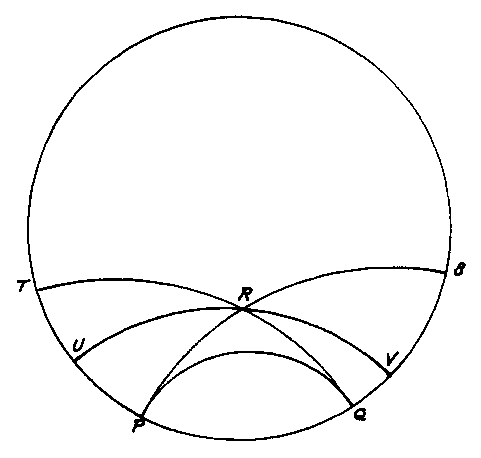
\includegraphics{chap02-vend-scan-06.eps}
\end{figure}

\noindent in hyperbolic geometry. For example, it is still true that the $H$-line which cuts the $H$-line $ab$ orthogonally at its midpoint is the locus of points equidistant from $a$ and $b$.


\subsection{}\label{ch02:sec12C} Hyperbolic geometry is the collection of those properties of sets in the hyperbolic plane that are unaltered by the transformations of a certain group of ``rigid motions.''\index{rigid motions} Certainly a rigid motion must preserve $\mathscr{U}$ and it is highly desirable that it send $H$-lines into $H$-lines. These requirements are met by the group of linear transformations of $\mathscr{U}$ on itself. Call this group $\Theta$; its elements are of the form (\ref{ch02:sec9E})
\begin{equation*}
z^{\prime}=Vz,\qquad V=\left(\begin{matrix}a & \bar{c}\\c & \bar{a}\end{matrix}\right),\qquad a\bar{a}-c\bar{c}=1.
\end{equation*}

The term ``rigid motion'' implies the existence of a ``distance''\index{hyperbolic geometry!distance in} which is preserved by the rigid motion. Indeed Cayley\index{Cayley} defined a distance in $\mathscr{U}$ which has all the properties of a distance in a metric space and is moreover invariant under $\Theta$. Besides, this distance has the additivity property of distances measured along straight lines.

To define this distance, let $\lambda$ be the $H$-line through $w_{1}$ and $w_{2}$, two points of $\mathscr{U}$. $\lambda$ intersects $\mathscr{Q}$ in two points $\infty_{1}$ and $\infty_{2}$, so labelled that $\infty_{1},\, w_{1},\,w_{2},\,\infty_{2}$ are in order on $\lambda$. The cross ratio
\begin{equation*}
\chi=\frac{(w_{1}-\infty_{2})(w_{2}-\infty_{1})}{(w_{1}-\infty_{1})(w_{2}-\infty_{2})}
\end{equation*}
is real and $\chi>1$. Define the $H$-distance
\begin{equation}
\label{ch02:eqn19}
d(w_{1},\,w_{2})=\frac{1}{2}\log\,\chi >0.
\end{equation}
Since the cross ratio is invariant under linear transformations (\ref{ch02:sec9A}), the same is true of the distance $d$. That is, two points a certain $H$-distance apart are mapped by a linear transformation into two points the same $H$-distance apart. Moreover, two hyperbolic line segments can be mapped into each other by a rigid motion if and only if they have the same $H$-length.


\subsection{}\label{ch02:sec12D}
Let $w_{3}$ be a point on $\lambda$ lying between $w_{1}$ and $w_{2}$. Then the points at infinity are the same for the segments $w_{1}w_{3},\,w_{3}w_{2}$, and $w_{1}w_{2}$ and we calculate easily that
\begin{equation*}
d(w_{1},\,w_{3})+d(w_{3},\,w_{2})=d(w_{1},\,w_{2}),
\end{equation*}
that is, distance\index{hyperbolic geometry!distance in} along an $H$-line is additive.

Let $a>0$ and consider $d(0,\,a)$. Here $\infty_{1}=-1,\,\infty_{2}=1$ and so $d(0,\, a)=\log\{(1+a)/(1-a)\}$. Since $a$ can be carried into $ae^{i\theta}$ by a rotation which leaves $0$ fixed (a rigid motion), we have
\begin{equation}
\label{ch02:eqn20}
d(0,\,ae^{i\theta})=\frac{1}{2}\log\frac{1+a}{1-a},\qquad0<a<1.
\end{equation}

An $H$-circle with center $w_{0}$ and radius $r$ is the locus of $H$-points at an $H$-distance $r$ from $w_{0}$. Map $w_{0}$ into $0$ by a rigid motion; the $H$-circle is mapped into an $H$-circle about $0$ of radius $r$. But this is a euclidean circle about $0$ of radius $\log\{(1+r)/(1\,-r)\}$. Map 0 back to $w_{0}$; the euclidean circle goes into another euclidean circle. Hence the $H$-circle is a euclidean circle lying in $\mathscr{U}$.

Another expression for the distance, one not involving the infinite points, is
\begin{equation*}
d(w_{1},\,w_{2})\, =\frac{1}{2}\log\frac{1+|(w_{2}-w_{1})/(1-\overline{w}_{1}w_{2})|}{1-|(w_{2}-w_{1})/(1-\overline{w}_{1}w_{2})|}
\end{equation*}


\subsection{}\label{ch02:sec12E} It can be shown that $\mathscr{U}$ is \emph{a metric space under the distance }$d(w_{1},\,w_{2})$. In a metric space a compact set is bounded. If $K$ is a compact subset of $\mathscr{U},d(0,\,w)\leqq R<\infty$ for each $w$. in $k$.


\subsection{}\label{ch02:sec12F} We shall need certain invariant differentials\index{invariant differential}. Differentiate $z^{\prime}=Vz$ with $V\in\Theta$ (cf. (\ref{ch02:sec12C}):
\begin{equation*}
|d\,Vz|=\frac{|dz|}{|cz+\bar{a}|^{2}}.
\end{equation*}
Also we verify directly that
\begin{equation}
\label{ch02:eqn21}
1-|Vz|^{2}=1-Vz\cdot\overline{Vz}=\frac{1-|z|^{2}}{|cz+\bar{a}|^{2}}.
\end{equation}
Dividing the first equation by the second, we get
\begin{equation}
\label{ch02:eqn22}
\frac{|d\,Vz|}{1-|Vz|^{2}}=\frac{|dz|}{1-|z|^{2}},
\end{equation}
that is, the differential $|dz|/(1-|z|^{2})$ is invariant under rigid motions.

If $z=\rho e^{i\theta}$, it can be shown that the differential
\begin{equation}
\label{ch02:eqn23}
\rho\,d\,\rho\,d\theta/(1-\rho^{2})^{2}
\end{equation}
is also invariant under rigid motions. The expressions \eqref{ch02:eqn22} and \eqref{ch02:eqn23} are the differentials of $H$-length and $H$-area, respectively.


\subsection{}\label{ch02:sec12G} We now treat the half-plane model of hyperbolic geometry. Here the hyperbolic plane is represented by the upper half-plane\index{hyperbolic geometry!upper half-plane as model of}. $\mathscr{H}$: $\mathrm{Im}\,z>0$, hyperbolic lines are represented by arcs of circles orthogonal to the real axis, and the euclidean angle measure is retained. The rigid motions of $\mathscr{H}$ are the linear transformations $V=(a\,b|c\,d)$ of $\mathscr{H}$ on itself. $V$ has real entries (\ref{ch02:sec9E}). Distance\index{hyperbolic geometry!distance in} is defined as before: it is invariant under rigid motions, and $\mathscr{H}$ is a metric space with this distance. The invariant differential is obtained from the formulas
\begin{equation*}
|dz^{\prime}|=\frac{|dz|}{|cz+d|^{2}},\quad y^{\prime}=\frac{y}{|cz+d|^{2}}
\end{equation*}
where $z=x +iy,\,z^{\prime}=Vz=x^{\prime}+iy^{\prime}.$ Hence
\begin{equation}
\label{ch02:eqn24}
\frac{|dz^{\prime}|}{y^{\prime}}=\frac{|dz|}{y}.
\end{equation}
This is the differential of $H$-length. The differential of $H$-area is
\begin{equation}
\label{ch02:eqn25}
|dx\,dy|/y^{2}.
\end{equation}

Let $A$ be a linear transformation mapping $\mathscr{U}$ on $\mathscr{H}$. Let $w_{1},w_{2}\in \mathscr{U}.$ Then
\begin{equation*}
d(w_{1},\,w_{2})=d^{\prime}(Aw_{1},\,Aw_{2}),
\end{equation*}
where $d,\,d^{\prime}$ are the hyperbolic distances in $\mathscr{U}$ and $\mathscr{H}$, respectively. For the $H$-line connecting $w_{1}, w_{2}$ is mapped onto the $H$-line connecting $Aw_{1},\,Aw_{2}$ and the cross ratio is preserved.


\subsection{}\label{ch02:sec12H}
An $H$-\emph{convex set} is a subset of $\mathscr{U}$ (or $\mathscr{H}$) which contains the $H$-line segment joining any two of its points. A region which is $H$-convex is called an $H$-\emph{convex region}\index{$H$-convex}. We list some well-known properties of $H$-convex sets.

1) An $H$-convex set is connected.

2) The intersection of a collection of $H$-convex sets (regions) is an $H$-convex set (region).

3) The interior of an $H$-convex set is an $H$-convex region.

\textsc{References}: \citeauthor{Caratheodory0000}~[\ref{Caratheodory1}]\index{Carath\'{e}odory}, Ch. \ref{ch03:chap03}; \citeauthor{Nevanlinna0000}~[\ref{Nevanlinna1}]\index{Nevanlinn}, pp. 217--219; \citeauthor{Springer0000}~[\ref{Springer1}],\index{Springer} pp. 230-235.


\skiptoctrue
\section*{Exercise}

1. In the hyperbolic geometry of the upper half-plane the $H$-circle of radius $\rho$ with center $x_{0}+iy_{0},\,y_{0} >0$, has the equation
\begin{equation*}
(x-x_{0})^{2}+(y-y_{0}\,\cosh \rho)^{2}=y_{0}^{2}\,\sinh\cdot^{2}\rho.
\end{equation*}
The hyperbolic area of this circle is 4 $\sinh\,{^{2}}\rho$.

\section{Miscellaneous}\label{ch02:sec13}

\subsection{}\label{ch02:sec13A}
A \emph{module} is a set of complex numbers that contains the sum and difference of any two of its elements. A module is \emph{discrete}\index{discrete module} if it has no finite points of accumulation.

\begin{theorem*}
A discrete module containing numbers other than $0$ has a basis consisting of two elements, $\omega_{1},\,\omega_{2}$, whose ratio is not real. That is, every number $z$ in the module is of the form
\begin{equation*}
z=m_{1}\omega_{1}+m_{2}\omega_{2}
\end{equation*}
with rational integral $m_{1},\,m_{2}$.
\end{theorem*}

Cf. \citeauthor{Hurwitz0000}\index{Hurwitz-Courant} [\ref{Hurwitz}], pp. 149--153.


\subsection{}\label{ch02:sec13B}
\textsc{Dirichlet's theorem}. If $\theta$ is a\index{Dirichlet's theorem} real irrational number, the set
\begin{equation*}
\{m+n\theta|m,\,n=\mathrm{integer}\}
\end{equation*}
is dense in the set of real numbers.

Cf. \citeauthor{Hardy0000b}\index{Hardy-Wright} [\ref{Hardy1a}], p. 375.


\subsection{}\label{ch02:sec13C} We sketch very briefly the elements of the Lebesgue theory\index{Lebesgue theory} of integration.

A subset $S$ of the real line $E$ is said to be of measure 0---we write $mS=0$--- if $S$ can be covered by a countable collection of intervals of arbitrarily small total length. A property defined for $x\in S$ is said to hold \emph{almost everywhere} in $S$ or for \emph{almost all} $x$ in $S$ provided it holds for $x \in T$ such that $m(S-T)=0$.

The Lebesgue theory distinguishes a class of subsets of $E$ called \emph{measurable}, including, in particular, the open sets and the complements and countable unions of measurable sets. A real-valued function $f$ is then called measurable if the set $\{x|f(x)>c\}$ is a measurable set for each real number $c$. In particular, continuous functions are measurable. The integral of $f$ over $S,\,\int_{S}f(x)dx =\int_{S}f$, is defined for measurable sets $S$ and measurable functions $f$. For a complex-valued $f=u+iv$ we simply define $\int_{S}f=\int_{S}u+i\int_{S}v$.

The function $f$ is \emph{integrable} over $S$ if $\int_{S}f$ is finite. We have $\int_{S}f=\int_{S^{\prime}}f$ if the set $(S\,-S^{\prime})\bigcup (S^{\prime}-S)$ is of measure zero. A sufficient condition that $f$ be integrable over $S$ is that $|f(x)|<g(x)$ for some function $g$ integrable over $S$.

The linearity of the integral is familiar. Besides this, the following properties should be mentioned.

\textsc{Complete additivity}. \emph{Let $\{S_{n}\}$ be a denumerable disjoint family of measurable sets; let $S=\bigcup_{1}^{\infty}S_{n}$. If $f$ is integrable over $S$,}
\begin{equation*}
\int_{S}f=\sum\limits_{n=1}^{\infty}\int_{S_{n}}f.
\end{equation*}

\textsc{Lebesgue's convergence theorem}. \emph{If} $f_{n}(x),\,n=1,\,2,\cdots$ \emph{is defined over} $S$ \emph{and is measurable, and if there exists a function} $g$ \emph{integrable over} $S$ \emph{such that}
\begin{equation*}
\sum\limits_{n=1}^{\infty}|f_{n}(x)|\leqq g(x)\ almost\ everywhere\ in\ S,
\end{equation*}
\emph{and the series} $f_{n}(x)$ \emph{converges almost everywhere then}
\begin{equation*}
\int_{S}dx\sum\limits_{n=1}^{\infty}f_{n}(x)=\sum\limits_{n=1}^{\infty}\int_{S}f_{n}(x)dx.
\end{equation*}

\textsc{Integration by parts}. \emph{Suppose} $f,\,g$ \emph{are summable over the interval} $(a,\,b)$; \emph{set}
\begin{equation*}
F(x)=\int_{a}^{x}f(t)dt,\qquad G(x)=\int_{a}^{x}g(t)dt.
\end{equation*}
\emph{Then}
\begin{equation*}
\int_{a}^{b}F(x)g(x)dx=FG\bigg|_{a}^{b}-\int_{a}^{b}G(x)f(x)dx.
\end{equation*}

\textsc{Change of variable}. \emph{Assume} $x(t)$ \emph{is nondecreasing in the interval} $\alpha\leqq t \leqq\beta$; \emph{as a consequence} $x^{\prime}(t)$ \emph{exists almost everywhere in this interval} (Lebesgue's Theorem; cf. \citeauthor{Riesz0000}\index{Rieaz-Nagy} [\ref{Riesz}, p. 5]). \emph{Assume also} $x(t)$ \emph{is absolutely continuous in} $(\alpha,\,\beta)$, i.e., $x(t)$ \emph{is the indefinite integral of an integrable function. Let} $x(t)$ \emph{map} $(\alpha,\,\beta)$ \emph{onto an interval} $(a,\,b)$. \emph{Then}
\begin{equation*}
\int_{a}^{b}f(x)dx=\int_{a}^{\beta}f(x(t))x^{\prime}(t)dt.
\end{equation*}

The Lebesgue theory extends immediately to euclidean spaces of higher dimension. An open plane subset together with some or all of its boundary is measurable. For functions of two variables we have the essential

\textsc{Fubini's theorem}. \emph{If a function} $f(x,\,y)$ \emph{is integrable over a rectangle} $R$: $a<x<b,\,c<y<d$, \emph{then}
\begin{equation*}
\iint\limits_{R}f(x,\,y)dxdy=\int_{a}^{b}\bigg\{\int_{c}^{d}f(x,\,y)dy\bigg\}dx=\int_{c}^{d}\bigg\{\int_{a}^{b}f(x,\, y)dx\bigg\}dy.
\end{equation*}
Cf. \citeauthor{Riesz0000} [\ref{Riesz}], Ch. \ref{ch02:chap02}; \citeauthor{Titchmarsh0000}~[\ref{Titchmarsh1}]\index{Titchmarsh}, Chs. \ref{ch10:chap10}, \ref{ch12:chap12}.


%%%%%%%%%%chapter03

\chapter{Discontinuous Groups}\label{ch03:chap03}\index{discontinuous group}

The concept of discontinuity can be defined for a group $G$ of 1-1 mappings of a topological space $X$ on itself. We say $G$ is discontinuous at a point $x\in X$ if there is no $y \in X$ and no sequence of distinct $V_{n}\in G$ for which $V_{n}y\rightarrow r$.

In this book, however, we shall be concerned entirely with groups of \emph{analytic} homeomorphisms of the complex sphere.\footnote{In the lost chapter only we consider groups on complex spaces of higher dimension.} We impose the restriction of analyticity because we wish to construct automorphic functions, that is, analytic functions invariant on $G$. From $f\circ V =f$ with $f$ analytic and $V\in G$ we can deduce that $V$ is analytic. According to \ref{ch02:chap02}. Th. \ref{ch02:sec8D} analytic (i.e., a directly conformal) 1-1 mapping of the sphere is a linear transformation.

It may be asked why we do not consider the group of analytic homeomorphisms of an arbitrary region $\mathscr{D}$. The fact is that the general case reduces essentially to the one we are treating. A simply connected $\mathscr{D}$ is conformally equivalent to a normal region $E$ (sphere, plane, or disk). The analytic 1-1 mappings of $E$ are known to be linear transformations. Thus if $G$ is a group of self-mappings of $\mathscr{D}$ and $\varphi(\mathscr{D})= E, G^{\prime} = \varphi \circ G \circ\varphi^{-1}$ is the corresponding group for $E$ and consists of linear transformations. The study of $G^{\prime}$ is equivalent to the study of $G$ but is far easier. A doubly connected $\mathscr{D}$ is conformally equivalent to an annulus, whose conformal mappings are rotations about the center. Regions of higher connectivity possess very few self-mappings other than the identity, and in any case only a finite number (\citeauthor{Julia0000}~[\ref{Julia1}\index{Julia}, p. 68]). These are the only groups that are possibly not conjugate to a group of linear transformations.

The material in this chapter, roughly speaking, is what may be derived by group-theoretic and topological means. In the next chapter we introduce the fundamental region, a geometric tool of the highest interest and applicability.

\section{Discontinuity}\label{ch03:sec1}

\subsection{}\label{ch03:sec1A} Let $\Omega$ be the group of all conformal homeomorphisms of the complex sphere $\mathscr{Z}$. Each element of $\Omega$ is a linear transformation
\begin{equation}
\label{ch03:eqn1}
z^{\prime}=Tz=\frac{az+b}{cz+d},\quad ad-bc =1
\end{equation}
where $a,\,b,\,c,\,d$ are complex numbers (\ref{ch02:chap02}. Th. \ref{ch02:sec8D}). The elements of $\Omega$ will be referred to as elements, transformations, or substitutions. As we did in Chapter~\ref{ch02:chap02} we use the letter $T$ to denote both the matrix $(a\,b|c\,d)$ and the transformation (1), but it must be remembered that the matrices $T$ and $-T$ give rise to the same transformation.


\begin{definition*}
Two subsets $A,\,B$ of $\mathscr{Z}$ are said to be \emph{equivalent under} $\Omega$ (or $\Omega$-\emph{equivalent}) if there is a $T\in\Omega$ such that
\begin{equation*}
TA=B.
\end{equation*}
The definition is most frequently applied to the case in which $A$ and $B$ are single points.
\end{definition*}

\subsection{}\label{ch03:sec1B} We wish to investigate subgroups of $\Omega$ having the property known as \emph{discontinuity}.


\begin{definition*}
Let $\Gamma$ be a subgroup of $\Omega$. The point $\alpha$ is called a \emph{limit point}\index{$\mathscr{L}$= set of limit points} of $\Gamma$ provided there is a point $z$ and an infinite sequence $\{V_{n}\}$ of different elements of $\Gamma$ such that $V_{n}z\rightarrow\alpha$. If $\alpha$ is not a limit point, it is an \emph{ordinary point} of $\Gamma$.

It is important to note that the images $\{V_{n}z\}$ need not be distinct. Thus a point $\alpha$ which is a fixed point of infinitely many different $V\in\Gamma$ is a limit point of $\Gamma$.
\end{definition*}

\begin{definition*}
$\Gamma$ is said to be discontinuous at a point\index{discontinuous at a point} $\alpha$ if $\alpha$ is an ordinary point of $\Gamma$. It is said to be discontinuous in a set\index{discontinuous in a set} $S$ if it is discontinuous at each point of $S$. A group is called a discontinuous group if it is discontinuous somewhere.

In this chapter we shall use the letter $\Gamma$ to denote a discontinuous group. That is, $\Gamma$ has at least one ordinary point.

Discontinuity of $\Gamma$ at $\alpha$ implies that \emph{the set} $\Gamma_{z}$ \emph{does not accumulate at} $\alpha$ \emph{no matter what} $z\in \mathscr{Z}$ \emph{may be}.
\end{definition*}

\subsection{}\label{ch03:sec1C} Denote by $\mathscr{L}$, or if necessary by $\mathscr{L}(\Gamma)$, the set of limit points\index{$\mathscr{L}$= set of limit points} of $\Gamma$ and by $\mathcal{O}$ the set of ordinary points\index{$\mathscr{O}$ = set of ordinary points}. By definition, $\mathscr{L}$ is the complement of $\mathcal{O}$.


\begin{theorem*}
For each $V\in \Gamma,\,V(\mathscr{L})=\mathscr{L}\ and\ V(\mathcal{O})=\mathcal{O}$.
\end{theorem*}

It is necessary to prove only the first statement. For if $V$ sends a point of $\mathcal{O}$ into a point of $\mathscr{L}$, then $V^{-1}$ sends a point of $\mathscr{L}$ into a point of $\mathcal{O}$, contradicting the first assertion.

Suppose $\lambda\in \mathscr{L}$. There is a sequence $V_{n}\,z\rightarrow\lambda,$ $V_{n}\in\Gamma$ and distinct. Then $VV_{n}\,z\rightarrow V\lambda$, since $V$ is continuous on the complex sphere. The $\{VV_{n}\}$ are all distinct since the $\{V_{n}\}$ are. Hence $\lambda\in \mathscr{L}$ implies $V\lambda\in \mathscr{L}$, or $V(\mathscr{L})\subset \mathscr{L}$. Since this is true for each $V\in\Gamma$, in particular for $V^{-1},$ we have $V^{-1}\mathscr{L}\subset\mathscr{L}$, whence $\mathscr{L}\subset V\mathscr{L}$.\:\:\:q.e.d.

\subsection{}\label{ch03:sec1D}
\setcounter{lemma}{0}
\begin{lemma}\label{ch03:lem1} If $\Delta$ is a subgroup of $\Gamma$, then $\mathcal{O}(\Gamma)\subset \mathcal{O}(\Delta).$ In particular, a subgroup of a discontinuous group is discontinuous.
\end{lemma}


\begin{lemma}\label{ch03:lem2} If $A$ is a nonsingular linear transformation, then $\mathcal{O}(A\Gamma A^{-1})=A\{\mathcal{O}(\Gamma)\}$ and $\mathscr{L}(A\Gamma A^{-1})=A\{\mathscr{L}(\Gamma)\}$.
\end{lemma}

The proofs of these lemmas are very easy and are left to the reader. We shall frequently use the second lemma to replace $\Gamma$ by a transformed group\index{transform of a group} in which we wish to assume, as a matter of convenience, that a certain point (such as $\infty$) is an ordinary point.

\subsection{}\label{ch03:sec1E} The simplest discontinuous groups are cyclic.


\begin{theorem*}
Let $\Gamma$ be the cyclic group generated by an element $T$. If $T$ is not elliptic, $\Gamma$ is discontinuous everywhere except at the fixed point, or fixed points, of $T$. If $T$ is elliptic, $\Gamma$ is discontinuous everywhere if $T$ is of finite order; it is discontinuous nowhere if $T$ is of infinite order.
\end{theorem*}

Since a fixed point of $T$ is a fixed point of all powers of $T$, a fixed point is clearly a limit point of $\Gamma$ if $T$ is not elliptic, for a nonelliptic transformation is of infinite order and all its powers are distinct (\ref{ch02:chap02}.~\ref{ch02:sec9C}). Every point $z_{0}$ different from a fixed point, however, is an ordinary point. Indeed, let $V_{n}z=T^{k_{n}}z\rightarrow z_{0}$ with $k_{n}\rightarrow\infty$. Then $z_{0}$ is a fixed point (\ref{ch02:chap02}. Ex. 9-3). This proves the first statement.

If $T$ is elliptic of finite order, the group generated by $T$ is finite and there can be no limit points. If $T$ is of infinite order, it is of the form\footnote{$e(\kappa)=e^{2\pi i\kappa}$.} $(z^{\prime}-z_{0})/(z^{\prime}-z_{1})=e(\kappa)\cdot(z\, -z_{0})/(z-z_{1}),\,\kappa$ irrational. By Dirichlet's theorem (\ref{ch02:chap02}.~\ref{ch02:sec13B}) there is a sequence of integers $n_{j}\rightarrow\infty$ such that $e(\kappa n_{j})\rightarrow 1$. Hence $T^{n_{j}}{z}\rightarrow z$, the $T^{n_{j}}$ being distinct. We see that $z$ is not an ordinary point of $\Gamma$. Since $z$ was arbitrary the result follows.

\subsection{}\label{ch03:sec1F} A less trivial example of a discontinuous group is the modular group\index{modular group},\footnote{The notation $\Gamma(1)$ will become more reasonable at the end of this subsection.} $\Gamma(1)$, the group of all unimodular matrices with rational integral entries. A transformation $V$ belonging to the modular group is called a modular substitution. $V$ maps\footnote{$\mathscr{H}$ is the upper half-plane.} $\mathscr{H}$ on itself, as we see immediately from the formula
\begin{equation*}
\mathrm{Im}\ V_{z}=y/|cz+d|^{2},\quad V=\left(\begin{matrix}\cdot & \cdot\\ c & d\end{matrix}\right),\quad z=x+iy.
\end{equation*}
Moreover, the modular group is discontinuous in $\mathscr{H}$. Suppose otherwise; let $z_{0}\in\mathscr{H}$ and let $\{V_{n}\}$ be a sequence of distinct modular substitutions such that $V_{n}z=x_{n}^{\prime}+iy^{\prime}_{n}\rightarrow z_{0}=x_{0}+iy_{0}$, where $z\in\mathscr{H}$. We discard those $V_{n}$, if any, for which the condition,
\begin{equation}
\tag{${^\ast}$}
-\frac{1}{2}\leqq\mathrm{Re}\,V_{n}z-\mathrm{Re}z_{0}<\frac{1}{2},
\end{equation}
is not satisfied. Now $y_{n}^{\prime}=y|c_{n}z+d_{n}|^{-2}\rightarrow y_{0}$. It follows that $(c_{n}x+d_{n})^{2}+c_{n}{^{2}}y^{2}$ is bounded, so that $c_{n}$ and $d_{n}$ are bounded. Therefore $c_{n}$, being an integer, assumes only a finite number of distinct values, likewise $d_{n}$. That is, there are only a finite number of pairs $(c_{n},\,d_{n})$ occurring as second row in the sequence $\{V_{n}\}$. Let $(c,\,d)$ be such a pair and $V= (a\,b|c\,d)$ a matrix in $\{V_{n}\}$. If $V^{\prime}=(a^{\prime}\,b^{\prime}|c\,d)$ is also in $\{V_{n}\}$, then $V^{\prime}V^{-1}=(\cdot\,\cdot|0\,1)$ and so must be $(1\,m|0\,1)$ for some integer $m$. It follows that $V^{\prime}= (a+mc,\,b+md|0\,1)$. But we required the condition $(^{\ast}$); since $V^{\prime}z= Vz+m$, there is just one value of $m$ for which this condition is satisfied. In other words, the matrix $V$ belonging to the sequence $\{V_{n}\}$ is uniquely determined by its second row. Our conclusion is that $\{V_{n}\}$ contains only finitely many matrices, a contradiction.

It is equally clear that the modular group is discontinuous in the lower half-plane. It also maps the real axis on itself, but it cannot be discontinuous at any real point $x$. Choose distinct pairs of relatively prime integers $b_{n},\,d_{n}$ so that $b_{n}/d_{n}\rightarrow x$. We then solve the equation $a_{n}d_{n}-b_{n}c_{n}=1$ in integers $a_{n},\,c_{n}$. Thus $V_{n}=(a_{n}\,b_{n}|c_{n}\,d_{n})$ are modular substitutions, the $V_{n}$ are distinct, and $V_{n}(0)\rightarrow x$.

We see then that $\Gamma(1)$ is discontinuous on the upper as well as the lower half-plane, but fails to be discontinuous at any real point.

Every subgroup of $\Gamma(1)$ is again discontinuous on $\mathscr{H}$, and the modular group has a great variety of subgroups. We mention at this point only \emph{the principal congruence subgroup modulo}\index{principal congruence subgroup} $n,\,\Gamma(n)$, defined as the set of all modular transformations such that
\begin{equation*}
\left(\begin{matrix}
a & b\\c & d
\end{matrix}\right)\equiv\pm\left(\begin{matrix}
1 & 0\\0 & 1
\end{matrix}\right)\,(\mathrm{mod}\,n).
\end{equation*}
It is readily verified that we have here a normal subgroup of finite index.


\subsection{}\label{ch03:sec1G} The prime topological property of $\mathcal{O}$ is that it is an open\index{$\mathscr{O}$ = set of ordinary points!is open} set.


\begin{theorem*}
$\mathcal{O}$ is open. $\mathscr{L}$ is closed\index{$\mathscr{L}$= set of limit points!is closed}.
\end{theorem*}

The proof of this theorem requires some results important in themselves.

\subsection{}\label{ch03:sec1H} \begin{theorem*} If $\infty$ is an ordinary point, and $V_{n}=(a_{n}\,b_{n}|c_{n}\,d_{n})$ a sequence of distinct elements of $\Gamma$, then $|c_{n}|\rightarrow\infty$.
\end{theorem*}


Suppose on the contrary there is a subsequence (still denoted by $V_{n}$) on which $c_{n}\rightarrow\gamma$ (finite). Since $\infty$ is an ordinary point, the sequences $(V_{{n}}^{-1}(\infty)=-d_{n}/c_{n}),\,(V_{n}(\infty)=a_{n}/c_{n})$, and $(V_{n}(0)=b_{n}/d_{n})$ are bounded for $n>N$. Hence, there is a subsequence $(p)$ on which they converge. Since $c_{p}\rightarrow\gamma$, there are numbers $\delta$ and $\alpha$ such that $d_{p}\rightarrow\delta,\, a_{p}\rightarrow\alpha$; this implies $b_{p}=(b_{p}/d_{p})d_{p}\rightarrow\beta$. Thus $V_{p}\rightarrow X=(\alpha\,\beta|\gamma\,\delta)$, and $\alpha\delta-\beta\gamma=1$, since $a_{p}d_{p}-b_{p}c_{p}=1$. $X$ is therefore nonsingular.

Let $w$ be an arbitrary point and $Xz=w$. The elements $V_{p}$ are distinct, by hypothesis. Since $V_{p}z\rightarrow Xz,\,\Gamma$ is not discontinuous at $w$. Hence $\Gamma$ is not a discontinuous group, a contradiction,\:\:\:q.e.d.

\subsection{}\label{ch03:sec1I} Assume $\infty$ is an ordinary point. Define
\begin{equation*}
\mathscr{L}_{\infty}=\{\mu|\quad\mu=\mathop{\lim}\limits_{n\rightarrow\infty}\quad V_{n}\infty,\quad V_{n}\,\mathrm{distinct},\quad V_{n}\in\Gamma\}.
\end{equation*}
Obviously $\mathscr{L}_{\infty}\subset\mathscr{L}$.


\setcounter{lemma}{0}
\begin{lemma}\label{ch03:lem1a}
$\mathscr{L}_{\infty}$ is closed.
\end{lemma}

This is a purely topological result. Let $\mu^{\ast}$ be an accumulation point of $\mathscr{L}_{\infty}$ and $\mu_{k}$ a member of $\mathscr{L}_{\infty}$ for which $|\mu^{\ast}-\mu_{k}|<1/k,\,k =1,2,\,\cdots$. Let $V_{n_{k}}$ be such that $|V_{n_{k}}\infty-\mu_{k}|<1/k$ and such that the $V_{n_{k}}$ are distinct. Then $|\mu^{\ast}-V_{n_{k}}\infty|<2/k\rightarrow 0$ with $k \rightarrow\infty$. Hence $\mu^{\ast}\in \mathscr{L}_{\infty}$.

\begin{lemma}\label{ch03:lem2a}
For each $V\in\Gamma,\,V(\mathscr{L}_{\infty})=\mathscr{L}_{\infty}$.
\end{lemma}

The proof is left to the reader.

\subsection{}\label{ch03:sec1J} \begin{theorem*} Assume $\infty$ is an ordinary point. Then $\mathscr{L}=\mathscr{L}_{\infty}$.
\end{theorem*}


Since we have already observed that $\mathscr{L}_{\infty}\subset\mathscr{L}$, we assume $\lambda\in \mathscr{L}$ and prove $\lambda\in \mathscr{L}_{\infty}$. Note that there are only finitely many $V_{n}=(a_{n}\,b_{n}|c_{n}\,d_{n})\in\Gamma$ for which $c_{n}=0$, for $\infty$ is fixed by such transformations and we have assumed $\infty$ to be ordinary. We discard these $V_{n}$ and assume from now on $c_{n}\neq 0$.

We have, for some $z$,
\begin{equation*}
\lambda=\lim_{n\rightarrow\infty}V_{n^{Z}},\quad V_{n}=\left(\begin{matrix}
a_{n} & b_{n}\\c_{n} & d_{n}
\end{matrix}\right)\in\Gamma.
\end{equation*}
Either
\begin{enumerate}
\item[1)] $|c_{n}z+d_{n}| \geqq 1$ for $n>N,$ or
\item[2)] $|c_{p}z+d_{p}| < 1$ on a subsequence $(p)\rightarrow \infty.$
\end{enumerate}

In case 1) we get
\begin{equation*}
|V_{n}z-V_{n}\infty|=\frac{1}{|c_{n}|\cdot|c_{n}z+d_{n}|}\leqq\frac{1}{|c_{n}|}\rightarrow 0
\end{equation*}
by Theorem 1H, so
\begin{equation*}
|\lambda-V_{n}\infty|\leqq|\lambda-V_{n}z|+|V_{n}z-V_{n}\infty|\rightarrow 0.
\end{equation*}
Hence $\lambda\in \mathscr{L}_{\infty}$.

In case 2), $z$ itself is in $\mathscr{L}_{\infty}$, for $|z+d_{p}/c_{p}|=|z-V_{p}^{-1}\infty|<1/|c_{p}|\rightarrow 0$. By~\ref{ch03:sec1I}, Lemma~\ref{ch03:lem2a}, $V_{n}z\in \mathscr{L}_{\infty}$ for each $n$. Hence $\lambda=\lim_{n\rightarrow\infty}V_{n}z$ is an accumulation point of $\mathscr{L}_{\infty}$, and so $\lambda$ is in $\mathscr{L}_{\infty}$ since the latter is closed.

In both cases, then, $\lambda\in \mathscr{L}_{\infty}$ and the proof is complete.

Suppose $\infty$ is an ordinary point. It is evident that the theorem we have just proved implies Theorem 1G If $\infty$ is not an ordinary point, let $A$ be a nonsingular linear transformation mapping some ordinary point on $\infty$. Then $A\Gamma A^{-1}$ has $\infty$ as an ordinary point and so $\mathscr{L}(A\Gamma A^{-1})$ is closed; this implies $\mathscr{L}(\Gamma)$ is closed (\ref{ch03:sec1D}, Lemma~\ref{ch03:lem2a}).

Theorem 1G is now completely proved.

\subsection{}\label{ch03:sec1K} \begin{theorem*} $\Gamma$ is a countable\index{discontinuous group!is countable} group.
\end{theorem*}


Cover each point of $\mathscr{O}$ by an open disk whose closure lies in $\mathcal{O}$, and from this open covering select a countable subcovering $\{\mathscr{O}_{n}\}$. (Lindel\"{o}f's Theorem states this is possible.) Then $\mathscr{O}\ =\cup_{n}K_{n},$ $n =1,2,\,\cdots$, where $K_{n}=\overline{\mathscr{O}}_{n}$. We enumerate the $V$ in $\Gamma$ by counting those $V$ for which $Vz_{0}\in K_{n},\,n =1,2,\cdots$, with $z_{0}$ an arbitrary point of $\mathscr{O}$. Each $V$ will be counted at least once, for $Vz_{0}$ is in $\mathscr{O}$ and hence in some $K_{n}$, possibly in several (Th. \ref{ch01:sec1C}). But there are only a finite number of such $V$ for each $n$. Indeed, $K_{n}$ is compact, and infinitely many $V_{k}z_{0}$ in $K_{n}$ would produce an accumulation point of the sequence $(V_{k}z_{0})$ lying in $K_{n}$, that is, in $\mathscr{O}$. Altogether, then, there are at most denumerably many $V$.

\subsection{}\label{ch03:sec1L} Our fundamental definition was that of a limit point of a group $G$. It can be stated in this way: $\lambda\in \mathscr{L}$ if and only if, for some $z,\,\lambda$ is an accumulation point of the \emph{sequence} $Gz$ (i.e., the sequence consisting of all the elements of $G)$. Other definitions have been used, for example: $\lambda$ is a limit point if and only if the \emph{set} $Gz$ is dense at $\lambda$. We shall briefly indicate the essential equivalence of the two definitions.

Suppose $G$ is discontinuous in our sense. Let
\begin{equation}
\tag{$^{\ast}$} \lambda=\lim_{n\rightarrow\infty}V_{n}z,\qquad V_{n}\in G,\quad \mathrm{distinct}.
\end{equation}
If infinitely many images $V_{n}z$ are different, $Gz$ is dense at $z$. If not, $\lambda$ is a fixed point of the infinite set $\{V_{n+1}V_{N}^{-1},\,n\geqq N\}$. Since this set is a subset of $G_{\lambda}$ (the subgroup of $G$ that fixes $\lambda$), $G_{\lambda}$ is infinite.

Provided $G_{\lambda}$ contains a nonelliptic element $S,\,Gz$ is dense at $\lambda$, for $S^{n}z\rightarrow\lambda$ with $n\rightarrow\infty$ or $n\rightarrow-\infty$ for all $z$ not coinciding with a fixed point of $S$. Assume, then, $G_{\lambda}$ contains only elliptic transformation; as we shall see in Theorem 2A, $G_{\lambda}$ is then finite, a contradiction.

Conversely, if $Gz$ is dense at $\lambda$ we can obviously construct a sequence $(^{*})$. \emph{In the case of a discontinuous group, the two definitions are equivalent}.

When $G$ is not discontinuous at any point, there is a slight anomaly, which can be avoided by assuming $G$ has no elliptic elements of infinite order. With this restriction, the definitions are equivalent.


\skiptoctrue
\section*{Exercises}

1. Let $C$ be the set of third entries in the matrices of $\Gamma$, i.e.,
\begin{equation*}
C=\bigg\{c\bigg|\exists\,\left(\begin{matrix}\cdot & \cdot\\ c & \cdot\end{matrix}\right)\in\Gamma\bigg\}.
\end{equation*}
Let $\infty$ be an ordinary point. Show that $C$ is a discrete set. Defining $\tilde{c}$\index{$\tilde{c}$} to be the minimum of $|c|$ taken over the nonzero elements of $C$, show that $\tilde{c}>0$. [Use Th. \ref{ch01:sec1H}.]

2. Prove: if $\infty$ is an ordinary point, there is only a finite number of $V= (a\,b|c\,d)\in\Gamma$ for which $c =\gamma$, a preassigned number.

3. If $\alpha$ is an ordinary point, $z$ an arbitrary point, then $Vz=\alpha$ for at most finitely many $V\in\Gamma$.

4. Let $\mathscr{F}$ be the set of fixed points of elements of $\Gamma$ other than the identity. Then $V\mathscr{F}=\mathscr{F}$ for each $V\in\Gamma$.

\section{The Transformations in a Discontinuous Group}\label{ch03:sec2}

The theorems of this section deal with the types of transformations which are present in a discontinuous group.

\subsection{}\label{ch03:sec2A} \begin{lemma*} $\Gamma$ contains no elliptic elements\index{groups with elliptic elements} of infinite order.
\end{lemma*}


An elliptic element of infinite order would generate a cyclic subgroup of $\Gamma$ which, according to Theorem 1E, is not discontinuous. By~\ref{ch03:sec1D}, Lemma~\ref{ch03:lem1a}, $\Gamma$ is not discontinuous.

\begin{theorem*}
If $\Gamma$ contains, besides the identity, only elliptic transformations, it is a finite group.
\end{theorem*}

If there are two substitutions $U,\,V$ with one but only one fixed point in common, then $UVU^{-1}V^{-1}$ is parabolic (\ref{ch02:chap02}.~\ref{ch02:sec9G}). Hence $U,\,V$ have either no common fixed point or else a common pair of fixed points.

Suppose there are an infinite number of $T_{i}\in\Gamma$ in the second category. We have just seen that the multiplier of an elliptic transformation in a discontinuous group is a root of unity $e(p/q),\,p,\,q$ integers, $q>0,\,(p,\,q)=1$. Let the multiplier of $T_{i}$ be $e(p_{i}/q_{i})$.

There are infinitely many distinct $T_{i}$, hence $q_{i}\rightarrow\infty$. When $e(p_{i}/q_{i})$ is a multiplier, so is $e(1/q_{i})$, for $T_{i}^{m_{i}}\in\Gamma$ and we can choose $m_{i}$ so that $p_{i}m_{i}\equiv 1(\mathrm{mod}\,q_{i})$, since $(p_{i},\,q_{i})=1$. Hence there is a sequence $(T_{k})$ whose multipliers tend to 1. Since all $T_{k}$ have the same fixed points, we see that $T_{k}z\rightarrow z$ for all $z$, which implies $\Gamma$ is not discontinuous.

Therefore we may discard the finite number of elements of $\Gamma$ that possess a common pair of fixed points and assume from now on that $U,\, V\in\Gamma$ implies $U$ and $V$ have no common fixed point. Let $U,\,V$ be transformed so that they appear as
\begin{equation*}
U=\left(\begin{matrix}
e(\theta) & 0\\0 & e(-\theta)
\end{matrix}\right),\quad0<\theta<1,\quad\theta\neq\frac{1}{2};\quad V=\left(\begin{matrix}
a & b\\c & d
\end{matrix}\right).
\end{equation*}
Since $V$ has neither $0$ nor $\infty$ as fixed point, we have $bc\neq 0$.

Now $UV$ is not the identity, otherwise $U$ and $V$ would have the same fixed points. Hence $UV$ is elliptic. Its trace $ae(\theta)+de(-\theta)$ is real, just as $a+d$ is. This gives $a=\overline{d}$.

But also the commutator $UVU\ {^1}V^{-1}$ is elliptic or the identity. Its trace is calculated as
\begin{equation*}
2(ad-bc\,\cos 2\pi\theta)=2(1+2bc\ \mathrm{sin}^{2}\,\pi\theta),
\end{equation*}
where we have used the equation $ad-bc=1$. Hence $bc$ is real and, in fact, $bc \leqq 0$. Hence $bc <0$.

Now $-\overline{c}/b=-c\overline{c}/cb>0$, set $|\mu|^{4}=-\overline{c}/b,\ \mu>0$. Then transform $\Gamma$ by $(\mu\,0|0\,\mu^{-1})$. The element $U$ remains the same under the transformation while $V$ becomes
\begin{equation*}
V=\left(\begin{matrix}\ \,a & e\\ {-}\bar{e} & \bar{a}\end{matrix}\right),\quad e=b\mu^{2}\neq 0.
\end{equation*}
Suppose $W=(\alpha\,\beta|\gamma\,\bar{\alpha})$ is another group element; then
\begin{equation*}
VW=\left(\begin{matrix}a\alpha+e\gamma & \cdot\\
\cdot & -\bar{e}\beta+\bar{a}\bar{\alpha}\end{matrix}\right)
\end{equation*}
must satisfy the condition $\overline{a\alpha+e\gamma}=-\bar{e}\beta+\bar{a}\bar{\alpha}$. Hence $\gamma=-\bar{\beta}$ (since $e\neq 0$) and $W$ is of the same form as $V$. That is, each element of $\Gamma$ is of the form
\begin{equation*}
R_{n}=\left(\begin{matrix}
\ \ a_{n} & b_{n}\\-\bar{b}_{n} & \bar{a}_{n}
\end{matrix}\right),\qquad a_{n}\bar{a}_{n}+b_{n}\bar{b}_{n}=1,\quad n=1,\,2,\,\cdots,
\end{equation*}
where $b_{n}$ is possibly $0$. Since $|a_{n}|\leqq 1,\,|b_{n}|\leqq 1$, there exist subsequences $a_{p}\rightarrow\alpha,\, b_{p}\rightarrow\beta$ and $R_{p}\rightarrow\ R=(\alpha\ \beta|-\bar{\beta}\ \bar{\alpha})$ with $R$ unimodular. Hence $R_{p}z\rightarrow Rz$, or $\Gamma$ is not discontinuous at $Rz$ for all $z \in \mathscr{F}$. Since $R$ maps $\mathscr{F}$ on itself, this shows that $\Gamma$ is nowhere discontinuous.

\subsection{}\label{ch03:sec2B}
\begin{theorem*} If $\Gamma$ contains only parabolic transformations, it contains only transformations having a common fixed point\index{fixed points of a group}.
\end{theorem*}


Let $V_{1}\in\Gamma,\,V_{1}\neq I$; transform $\Gamma$ so that the fixed point of $V_{1}$ is $\infty$. A parabolic element with fixed point $\infty$ is a translation. Thus $V_{1}= (1\,\lambda|0\,1),\,\lambda\neq 0$. Let $V_{2}$ be a transformation of $\Gamma$ not having the fixed point $\infty:V_{2}= (a\,b|c\,d),\,c\neq 0$. Consider
\begin{equation*}
S_{n}=V_{1}^{n}V_{2}=\left(\begin{matrix}{a}+n\lambda c & \cdot\\
\cdot & d\end{matrix}\right).
\end{equation*}
For sufficiently large $|n|$, the trace of $S_{n}$ is of absolute value greater than 2, since $\lambda c \neq 0$. Hence $S_{n}\in\Gamma$ is not parabolic,\:\:\:q.e.d.

From this theorem it is easy to deduce that the only discontinuous groups of exclusively parabolic elements\index{groups with parabolic elements} are the simply and doubly periodic\index{group!doubly periodic} groups. All elements of $\Gamma$ have a common fixed point, say $\infty$; they are all of the form: $z^{\prime}=z+\lambda$. The set of periods $\{\lambda\}$ is a module $M$, i.e., $M$ contains the sum and difference of any two of its elements. Moreover, $M$ is \emph{discrete} (has no finite points of accumulation), otherwise $\Gamma$ would not be discontinuous. Now a discrete module of complex numbers is either the set of integral multiples of one number $\sigma$ or the set of linear integral combinations of two complex numbers $\omega_{1},\,\omega_{2}$ whose ratio is not real (\ref{ch02:chap02}.~\ref{ch02:sec13A}). We get in the first case the simply periodic\index{group!simply periodic} group with period $\sigma$; in the second, the doubly periodic group with primitive periods $\omega_{1},\,\omega_{2}$.

\subsection{}\label{ch03:sec2C}
We turn now to groups containing elliptic and parabolic elements\index{groups with elliptic elements}\index{groups with parabolic elements}.


\begin{theorem*}
If $\Gamma$ is an infinite group consisting entirely of elliptic and parabolic substitutions all of which have a common fixed point\index{fixed points of a group}, then $\Gamma$ has the common point as its sole limit point.
\end{theorem*}

If $\Gamma$ contains only elliptic transformations, it cannot be infinite (Theorem 2A), and if it contains only parabolic transformations, the truth of the present theorem is evident. Hence we assume $\Gamma$ has elements of both types.

Assume the common fixed point is at $\infty$. The subgroup of parabolic elements of $\Gamma$ is the simply or doubly periodic group (\ref{ch03:sec2B}). Calling this subgroup $P$, we have
\begin{equation*}
P=\{T|Tz=z+\Omega,\quad\Omega=m\omega_{1}+n\omega_{2}\},
\end{equation*}
where $m,\,n$ are integers. Here $\omega_{1}$ is the period of minimum modulus and $\omega_{1}/\omega_{2}$ a is not real. $\omega_{2} =0$ if $P$ is the simply periodic group.

Let one of the elliptic elements of $\Gamma$ be
\begin{equation*}
V_{1}:z^{\prime}=\varepsilon z+b,\qquad|\varepsilon|=1.
\end{equation*}
Letting $S$ be the substitution $z^{\prime}=z+\omega_{1}$, we have
\begin{equation*}
V_{1}SV_{1}^{-1}z=z+\varepsilon \omega_{1},
\end{equation*}
so that $\varepsilon \omega_{1}$ is a period, hence also $\varepsilon \omega_{1}-\omega_{1}$. The smallest period being $\omega_{1}$, this gives
\begin{equation*}
|\varepsilon-1|\geqq 1.
\end{equation*}
This inequality is fulfilled by the multiplier of every elliptic element of $\Gamma$.

Each multiplier $\varepsilon$ is a root of unity (Lemma 2A). Now every power of $\varepsilon$ is also a multiplier, so we may assume $\varepsilon$ is of the form $\zeta =e(1/l)$ for some integer $l\geqq 2$. Since $|\zeta-1|=2|\sin\pi/l|$ and $|\zeta-1|\geqq 1$, we see that $l\leqq 6$. Hence there are only a finite number of possible multipliers in elliptic substitutions of $\Gamma$, say $\varepsilon_{1},\,\varepsilon_{2},\,\cdots,\,\varepsilon_{s}$.

Let $V_{1},\,V_{2}$ be elliptic substitutions with the same multiplier $\varepsilon_{i}$:
\begin{equation*}
V_{1}=\varepsilon_{i}z+b_{i},\qquad V_{2}=\varepsilon_{i}z+b_{i}^{\prime}.
\end{equation*}
Then $V_{1}V_{2}^{-1}z=z+b_{i}-b_{i}^{\prime}$; in other words $b_{i}-b_{i}^{\prime}$ is a period. It follows that every elliptic substitution of $\Gamma$ is in the set
\begin{equation*}
B:z^{\prime}=\varepsilon_{i}z+b_{i}+\Omega,\qquad i=1,2,\cdots, s.
\end{equation*}

Every substitution $U$ of $\Gamma$ is either parabolic or elliptic, that is, is either in $P$ or in $E$. It is clear that if $z$ is fixed, there are only finitely many images $Uz$ lying in any disk about the origin. This shows that $\infty$ is the only limit point of $\Gamma$.

\subsection{}\label{ch03:sec2D} The groups treated in the last theorem had no hyperbolic\index{groups with hyperbolic elements} or loxodromic\index{groups with loxodromic elements} substitutions. This is no longer possible where there is more than one limit point.\footnote{A complete classification of the groups with two or fewer limit points can be found in [\citeauthor{Ford0000}~\ref{Ford1}\index{Ford}, Ch. VI].}

\begin{theorem*} If $\mathscr{L}$\index{$\mathscr{L}$= set of limit points} has more than one point, $\Gamma$ contains hyperbolic or loxodromic substitutions.
\end{theorem*}

Assume $\Gamma$ contains only elliptic and parabolic elements. $\Gamma$ does not consist only of elliptic substitutions, for then it would be a finite group (Th. \ref{ch01:sec2A}) Let $T$ be a parabolic element whose fixed point may be assumed to be $\infty$. Then $T$ is a translation $(1\,\kappa|0\,1)$. Since $\mathscr{L}$ contains more than one point, there is certainly a substitution $V= (a\,b|c\,d)$ which does not fix $\infty$ (Th. \ref{ch01:sec2C}). Hence $c \neq 0$, and $T^{n}V=(a+nc\kappa\,.|.\,d)$ has trace of absolute value $>2$ if $|n|$ is sufficiently large. It follows that $T^{n}V$ is hyperbolic or loxodromic.

\subsection{}\label{ch03:sec2E}
\begin{theorem*}. Let $\Delta$ be an infinite group of linear transformations. Let $V\in \Delta$ be hyperbolic\index{groups with hyperbolic elements} or loxodromic\index{groups with loxodromic elements} and let $U\in\Delta$ be a substitution which has one and only one fixed point in common with $V$. Then $\Delta$ is not discontinuous.
\end{theorem*}


By transformation we may assume the fixed points of $V$ at $0$ and $\infty$, the latter being the common fixed point of $U$ and $V$. We have
\begin{equation*}
V=\left(\begin{matrix}
\alpha & 0\\0 & \alpha^{-1}
\end{matrix}\right),\quad|\alpha|\neq 1;\quad U =\left(\begin{matrix}
a & b\\0 & a^{-1}
\end{matrix}\right),\quad ab\neq 0.
\end{equation*}
The commutator of $U$ and $V^{n}$ is
\begin{equation*}
U\,V^{n}U^{-1}V^{-n}=C_{n}=\left(\begin{matrix}
1 & ab(1-\alpha^{2n})\\0 & 1
\end{matrix}\right)
\end{equation*}
and is in $\Delta$. Hence $C_{n}\rightarrow C=(1\,ab|0\,1)$ for $n\rightarrow\infty(|\alpha|<1)$ or $n\rightarrow -\infty(|\alpha|>1)$. If only a finite number of $C_{n}$ were different we would have $C_{n}=C$ for $n>N$. This is impossible since $|\alpha|\neq 1$ and $ab\neq 0$. Therefore, there are distinct $C_{p}$ such that $C_{p}z\rightarrow Cz$ for each $z$, and so $\Delta$ is not discontinuous.

\begin{corollary*} A fixed point of a parabolic element\index{groups with parabolic elements} of a discontinuous group is not a fixed point of a hyperbolic or loxodromic element.
\end{corollary*}

\subsection{}\label{ch03:sec2F}
As another corollary we get


\begin{theorem*}
Let $\Gamma$ be a discontinuous group all of whose elements have a common fixed point\index{fixed points of a group}. Then $\Gamma$ has at most two limit points.
\end{theorem*}

Assume the common fixed point is $\infty$. If $\Gamma$ contains only elliptic and parabolic substitutions, it has the unique limit point $\infty$, if it is an infinite group (Th. \ref{ch01:sec2C}). Suppose $\Gamma$ has hyperbolic or loxodromic elements. All of these must have the same fixed points, $\infty$ and $0$ say, otherwise $\Gamma$ is not discontinuous (Theorem 2E). By the same token every elliptic transformation has $0$ and $\infty$ as fixed points. The parabolic elements have fixed point $\infty$. Suppose $V_{n}z\rightarrow z_{0}\neq 0,\,\infty$. If $(V_{n})$ contains an infinite subsequence $(V_{p})$ of nonparabolic elements, we have $\kappa_{p}z\rightarrow z_{0}$. Clearly $z\neq 0,\, \infty$. Hence $\kappa_{p} \rightarrow z_{0}/z$ and $V_{p}\zeta=\kappa_{p}\zeta\rightarrow z_{0}\zeta/z$ for each $\zeta;$ $\Gamma$ is not discontinuous. If $(V_{n})$ contains only a finite number of nonparabolic elements, we have $z +\lambda_{n}\rightarrow z_{0},\,\lambda_{n}\rightarrow z_{0}-z$, and the same conclusion follows. Hence $0$ and $\infty$ are the only limit\index{$\mathscr{L}$= set of limit points} points.

\skiptoctrue
\section*{Exercises}

1. Let $\Gamma$ be a discontinuous group each of whose elements fixes the same pair of points. List all possibilities for $\Gamma$. [Note that $\Gamma=N\cup N\alpha$, where $N$ is the subgroup fixing each of the points individually, and $\alpha$ is an (elliptic) element interchanging the points. If $N$ is infinite, its limit set consists of the 2 points; all such groups can be found in \citeauthor{Ford0000}~[\ref{Ford1}], Ch. 6.]

2. Find all abelian discontinuous groups.

3. A finite discontinuous group of linear transformations of the unit disk on itself is cyclic or has two generators.

\section{Discreteness}\label{ch03:sec3}

The restricting condition of discontinuity can be defined when $\Gamma$ is an arbitrary group of 1-1 mappings of the plane on itself. If, as in our case, $\Gamma$ has a representation by matrices, it is natural to ask for a restriction on the matrix group which corresponds to discontinuity. Such a restriction is \emph{discreteness} (\ref{ch02:chap02}.~\ref{ch02:sec6A}). We recall that the matrix group $\Gamma$ can be made into a topological group: convergence of a sequence of matrices is equivalent to convergence of the matrix elements. We then say $\Gamma$ is discrete provided the identity is an isolated element, or equivalently, provided $\Gamma$ contains no convergent sequence of distinct elements (\ref{ch02:chap02}.~\ref{ch02:sec6C}).

In this section we shall investigate the relation between discontinuity and discreteness. We shall see that with few exceptions the two concepts are equivalent.

\subsection{}\label{ch03:sec3A} For the moment denote the group of matrices by $\Gamma$, the group of transformations by $\overline{\Gamma}$.

In a discrete group there is, in particular, no sequence of distinct elements $T_{n}\in\Gamma$ converging to the identity. This condition may be expressed in terms of the transformations $\overline{T}_{n}z\in\overline{\Gamma}$.


\begin{lemma*} If there is a sequence of different transformations $\overline{T}_{n}\in\overline{\Gamma}$ such that $\overline{T}_{n}z\rightarrow z$ for $3$ distinct values of $z$, then $\varepsilon_{n}T_{n}\rightarrow I$ for suitably chosen $\varepsilon_{n}=\pm 1$. Conversely if $T_{n}\rightarrow I$ or $T_{n}\rightarrow-I$, then $\overline{T}_{n}z \rightarrow z$ for all $z$.
\end{lemma*}

The first part of the lemma is implied by \ref{ch02:chap02}. Th. \ref{ch02:sec9H}. The converse follows from~\ref{ch02:chap02}.~\ref{ch02:sec11D}.

When $\overline{\Gamma}$ contains a sequence $\overline{T}_{n}$ of distinct transformations such that $\overline{T}_{n}z\rightarrow z$ for all $z$, we say that $\overline{\Gamma}$ contains \emph{infinitesimal transformations}\index{infinitesimal transformations}. The term was used by Poincar\'{e}\index{Poincar\'{e}} and Klein\index{Klein, F.}. The lemma shows that the discreteness of $\Gamma$ is equivalent to the nonexistence of infinitesimal transformations in $\overline{\Gamma}$.

\subsection{}\label{ch03:sec3B} We return to our previous notation in which no distinction was made between $\Gamma$ and $\overline{\Gamma}$, always remembering that the matrices $\pm V$ correspond to the same transformation $V_{z}$.


\subsection{}\label{ch03:sec3C} Our object is to explore the connection between discreteness and discontinuity. In one direction the situation is obvious.


\begin{theorem*} A discontinuous group is discrete.
\end{theorem*}
For by Lemma 3A. $T_{n}\rightarrow I$ or $T_{n}\rightarrow-I$ implies $T_{n}z\rightarrow z$ for each $z$, and $\Gamma$ cannot be discontinuous at any point $z$.

However, the converse of this theorem is not true, as we observe immediately.

The \emph{group of Picard}\index{group of Picard} is defined as the set of unimodular matrices whose entries are complex integers, $a +bi$, with $a,\,b$ rational integers. This group is clearly discrete since the complex integers lie discrete in the plane. Nevertheless, the group of Picard is not discontinuous. For it is not difficult to find a sequence of different $\alpha_{n}/\gamma_{n}$, quotients of relatively prime complex integers, which approaches any preassigned complex number $z$. Given $\alpha_{n},\,\gamma_{n}$, we can solve the equation $\alpha_{n}\delta_{n}-\beta_{n}\gamma_{n}=1$ in complex integers $\beta_{n},\, \delta_{n}$. The matrices $V_{n}=(\alpha_{n}\,\beta_{n}|\gamma_{n}\,\delta_{n}),\,n=1,\,2, \cdots$, then belong to the Picard group and $V_{n}(\infty)=\alpha_{n}/\gamma_{n}\rightarrow z$. Hence discreteness is not sufficient to imply discontinuity.

\subsection{}\label{ch03:sec3D} We mention here without proof a result which, in one sense, solves the problem: a discrete group has a faithful representation by a discontinuous group of linear transformation of a half-space, for example, $\mathscr{H}_{3}= \{(x,\,y,\,z)|z>0\}$. Cf. \citeauthor{Fricke0000a}\index{Fricke-Klein} [\ref{Fricke1a}, p. 98]; [\citeauthor{Fatou0000}~\ref{Fatou1}\index{Fatou}, p. 86].


\subsection{}\label{ch03:sec3E}
If we remain in the plane, however, we must still look for necessary and sufficient conditions that $\Gamma$ be discontinuous. For this purpose we introduce the notion of a \emph{normal family of functions}\index{normal family of functions} (\citeauthor{Montel0000}~[\ref{Montel1}]\index{Montel}).

Let $\mathscr{D}$ be a region. If $\mathscr{D}$ is unbounded, call $\mathscr{D}_{1}$ and $\mathscr{D}_{2}$ the parts of $\mathscr{D}$ interior and exterior to the circle $|z|=1$, and call $\mathscr{D}_{2}$ the bounded region obtained by applying $z\rightarrow1/z$ to $\mathscr{D}_{2}$. Let $f_{n}(z)$ be a sequence of functions defined in $\mathscr{D}$ and let $g_{n}(z)=f_{n}(1\,/z)$. We say $f_{n}$ converges in $\mathscr{D}$ if $f_{n}(z)$ converges in $\mathscr{D}_{1}$ and $g_{n}(z)$ converges in $\mathscr{D}_{2}$. Also, we say that $f_{n}(z)\rightarrow\infty$ provided $1/f_{n}(z)\rightarrow 0$.


\begin{definition*}
A family\footnote{The family may have any cardinality.} of functions $\{f_{i}(z)\}$ meromorphic in a region $\mathscr{D}$ is said to bo normal in $\mathscr{D}$ provided that every infinite subset of $\{f_{i}\}$ contains a sequence of different functions $f_{n}(z)$ converging uniformly on compact subsets of $\mathscr{D}$ to a limit function $f(z)$ or to $\infty$. The family is said to be normal at a point provided it is normal in some region containing the point.

Obviously a subfamily of a normal family is normal. The normality of a family is not affected by dropping a finite number of its members. A family normal in $\mathscr{D}$ is normal in any subregion $\mathscr{D}^{\prime}$.
\end{definition*}

\begin{lemma*} If $\{f_{i}(z)\}$ is a normal family in $\mathscr{D}$ and A is a nonsingular linear transformation, then $\{A\circ f_{i}\circ A^{-1}(z)\}$ is normal in $A\mathscr{D}$.
\end{lemma*}

The proof is left to the reader.

\subsection{}\label{ch03:sec3F}
Fundamental in the study of normal families\index{normal family of functions} is the theorem of Montel\index{Montel} giving a sufficient condition for normality. We need, and shall prove, only a special case of this result.


\begin{lemma*} Let $\mathscr{D}$ be a region and $\rho,\,\sigma$ arbitrary, distinct complex numbers. Let $\{T_{i}(z)\}$ be a family of nonsingular linear transformations such that $T_{i}(z) \neq \rho,\,T_{i}(z)\neq \sigma$ for $z\in \mathscr{D}$. Then $\{T_{i}(z)\}$ is normal in $\mathscr{D}$.
\end{lemma*}

Set
\begin{equation*}
U_{i}(z)=\frac{T_{i}(z)-\rho}{T_{i}(z)-\sigma};
\end{equation*}
then $U_{i}$ is meromorphic in $\mathscr{D}$ and never assumes the values $0$ or $\infty$. Write $U_{i}=(a_{i}\,b_{i}|c_{i}\,d_{i})$.

We may assume that $\mathscr{D}$ contains the origin; if it doesn't we consider $\{U_{i}(z-z_{0})\}$. Let $K$ be a disk $|z|<R$ contained in $\mathscr{D}$ and let $R^{\prime}<R$. Since $U_{i}^{-1}(0),\, U_{i}^{-1}(\infty)$ do not lie in $K$, we have $|-b_{i}/a_{i}|>R,\,|-d_{i}/c_{i}|>R$. Write (Cf. Note 1, p. 399).
\begin{equation*}
U_{i}(z)=\frac{b_{i}}{d_{i}}\frac{z+b_{i}/a_{i}}{b_{i}/a_{i}}\frac{d_{i}/c_{i}}{z+d_{i}/c_{i}}=\frac{b_{i}}{d_{i}}W_{i}(z).
\end{equation*}
Then for $|z|\leqq R^{\prime}$ we have
\begin{equation*}
 0<\bigg(1-\frac{R^{\prime}}{R}\bigg)\frac{1}{1+R^{\prime}/R}\leqq\big|W_{i}(z)\big|\leqq\bigg(\frac{R^{\prime}}{R}+1\bigg)\frac{1}{1-R^{\prime}/R}<\infty.
\end{equation*}

If 1) $|b_{i}/d_{i}|<M$, then $|U_{i}(z)|\leqq M_{1}(R,\,R^{\prime})$ for $|z|\leqq R^{\prime}$ ; otherwise

2) there is a sequence on which $|b_{n}/d_{n}|\rightarrow\infty$ and $|1/U_{n}(z)|< |d_{n}/b_{n}|\cdot M_{2}(R,\,R^{\prime})\rightarrow 0$ with $n\rightarrow\infty$ uniformly in $|z|\leqq R^{\prime}$. Here $M_{1},\,M_{2}$ are functions of $(R,\,R^{\prime})$ but are independent of $n$.

Let $\mathscr{D}^{\prime}$ be an arbitrary compact subset of $\mathscr{D}$. Cover $\mathscr{D}^{\prime}$ by a finite number of disks $K_{j}^{\prime}$ of radius $R_{j}^{\prime}$ such that $K^{\prime}_{j}\subset \mathscr{D}$. In each $K_{j}^{\prime}$ we shall have estimates corresponding to 1) or 2) with $R,\,R^{\prime}$ replaced by $R_{j},\,R_{j}^{\prime}$.

Whether we have 1) or 2) does not depend on $j$ but only on the set $\{b_{i}/d_{i}\}$.

Therefore, we have either
\begin{enumerate}
\item[3)] $|U_{i}(z)|\leqq M$ for $z\in \mathscr{D}^{\prime}$, or
\item[4)] $|1/U_{n}(z)|\rightarrow 0$ uniformly for $z \in \mathscr{D}^{\prime}$,
\end{enumerate}
where $M$ depends only on $\mathscr{D}^{\prime}$. Now from a family of regular functions uniformly bounded in a region we can extract a uniformly convergent sequence (\ref{ch02:chap02}.~\ref{ch02:sec7F}). Hence in case 3) we obtain a convergent sequence $U_{p}(z)$, in case 4) we have $|U_{n}(z)|\rightarrow\infty$, and the convergence is uniform on each compact subset of $\mathscr{D}^{\prime}$, hence of $\mathscr{D}$. This shows the normality of $\{U_{i}(z)\}$ if $\mathscr{D}$ is bounded. An unbounded region is handled as indicated in~\ref{ch03:sec3E}.\:\:\:q.e.d.

This lemma will be used in the contrapositive form: \emph{if the family $\{T_{i}(z)\}$ is not normal in any region about a point $\beta$, then, with at most one exception $w_{0}$, there is a sequence of distinct $T_{n}\in\{T_{i}\}$ and a sequence $z_{n}\rightarrow\beta$ such that $T_{n}z_{n}=w,\,w \neq w_{0}$.} Indeed, let $N_{1}\supset N_{2}\supset\cdots$ be a sequence of regions containing $\beta$ and converging to $\beta$. Since $\{T_{i}\}$ is not normal in $N_{1}$, tho set $\{T_{i}(N_{1})\}$ cannot omit two distinct points by the lemma just proved. Hence there is a $z_{1}\in N_{1}$ and a $T_{1}$ such that $T_{1}z_{1}=w,\,w\neq w_{0}$. Now the family $\Omega_{1} =\{T_{i}\}-T_{1}$ is not normal in $N_{2}$. The set of values $\{T(N_{2})|T\in\Omega_{1}\}$ must contain $w$, otherwise this set would omit both $w$ and $w_{0}$ and $\Omega_{1}$ would be normal in $N_{2}$. Hence there is a $z_{2}\in N_{2}$ and $T_{2}\neq T_{1}$ for which $T_{2}z_{2}=w$. The continuation of this process leads to the desired sequence $(T_{n},\,z_{n})$. (Cf. Note 2, p. 399.)

\subsection{}\label{ch03:sec3G}
Now we can establish the main theorem.


\begin{theorem*}
A necessary and sufficient condition\index{discontinuous at a point!necessary and sufficient conditions} that $\Gamma$ be discontinuous at a point $\alpha$ is that
\begin{enumerate}
\item[1)] $\Gamma$ be discrete,
\item[2)] the functions $\{V(z),\,V\in\Gamma\}$ form a normal family in some disk $\mathscr{D}$ containing $\alpha$.
\end{enumerate}
\end{theorem*}

\emph{Proof of Necessity}. We may assume $\Gamma$ to be an infinite group, the result being trivial otherwise. We have already seen (Th. \ref{ch02:sec13C}) that $\Gamma$ is discrete. Now suppose $\Gamma=\{V(z)\}$ is not a normal family in any disk containing $\alpha$. Then by Lemma 3F (contrapositive form) there is a number $w$, a sequence of different elements $V_{n}$, and a sequence $z_{n}\rightarrow\alpha$, such that $V_{n}z_{n}=w$. Hence $z_{n}=V_{n}^{-1}w\rightarrow\alpha$ and this contradicts the discontinuity of $\Gamma$ at $\alpha$.

\emph{Proof of Sufficiency}. We start the sufficiency proof with a

\begin{lemma*} If $\{V_{n}z|V_{n}\in\Gamma\}$ is a family of distinct transformations converging uniformly in a compact region $\overline{\mathscr{D}}$ and $\Gamma$ is discrete, then $\varphi(z)=\lim_{n\rightarrow\infty}V_{n}z$ is a constant.
\end{lemma*}

By \ref{ch02:chap02}. Th. \ref{ch02:sec9H}, $\varphi(z)$ is a linear transformation if it is not a constant, and $V_{n}\rightarrow\Phi$, the matrix associated with $\varphi(z)$. Hence the sequence $(V_{n})$ converges, the $V_{n}$ being distinct, and so $\Gamma$ is not discrete.\:\:\:q.e.d.

We may assume $\alpha$ is a finite point, otherwise we transform the group (Lemma 3E). Now suppose $\Gamma$ is not discontinuous at $\alpha$ and let $z_{0}$ and $V_{n}\in\Gamma$ be such that $V_{n}z_{0}\rightarrow \alpha$ ($V_{n}$ distinct). Choose a substitution $V_{\mathrm{N}}\in\{V_{n}\}$ for which $V_{N}z_{0}=z_{1}\in \mathscr{D}$; let $T_{n}=V_{n}V_{N}^{-1}.$ Then $T_{n}z_{1}\rightarrow \alpha$. Now $\{T_{n}\}=\Gamma$ and so by hypothesis is normal in $\mathscr{D}$. Let $\{T_{p}\}$ be a subsequence which converges uniformly in $\overline{\mathscr{D}}_{1}\subset \mathscr{D}$, where $\overline{\mathscr{D}_{1}}$ contains $z_{1}$.

By the lemma just proved $\{T_{p}\}$ must converge to a constant; this constant can only be $\alpha$, since $T_{p}z_{1}\rightarrow\alpha$ and $z_{1}\in\overline{\mathscr{D}}_{1}$. Since the convergence is uniform it follows that there is a $p_{0}$ sufficiently large so that $T_{p_{0}}(\overline{\mathscr{D}}_{1})$ is a proper subset of $\overline{\mathscr{D}}_{1}$. Under these circumstances we know that $T_{p_{0}}$ is hyperbolic or loxodromic and that $T_{p_{0}}(\overline{\mathscr{D}}_{1})$ encloses a fixed point $\beta$ of $T_{p_{0}}$ (\ref{ch02:chap02}.~\ref{ch02:sec9I}).

But the family $\{T^{n}_{p_{n}}(z), n=1,\,2,\cdots\}$ cannot be normal in any region containing such a fixed point. Let $\gamma$ be the other fixed point of $T_{p_{0}}$ and write the powers
\begin{equation*}
T^{n}_{p_{0}}:\frac{z^{\prime}-\beta}{z^{\prime}-\gamma}=k^{n}\frac{z-\beta}{z-\gamma},\quad |k|\neq 1.
\end{equation*}
Now, for every $z\neq\beta,\, T^{n}_{p_{0}}(z)\rightarrow\gamma$ as $n \rightarrow\infty$ (if $|k|>1)$ or $n\rightarrow-\infty$ (if $|k|< 1)$. But $T^{n}_{p_{0}}(\beta)=\beta\neq\gamma$. The convergence cannot be uniform $\{T^{n}_{p_{0}}(z)\}$ is not normal in $\overline{\mathscr{D}}_{1}$. Then neither is $\Gamma-$ for a subfamily of a normal family is normal and this contradicts the hypothesis.

\subsection{}\label{ch03:sec3H} We are now able to state to a sufficient condition under which discreteness\index{discontinuity!and discreteness} implies discontinuity.


\begin{theorem*}Let $\Gamma$ be a discrete group of linear transformations. Then $\Gamma$ is discontinuous at each point $z$ which is covered by a disk $K$ such that $\Gamma K$ omits at least two points of the complex sphere. Moreover, $\Gamma$ is discontinuous in an open set $A$ if $\Gamma A \subset A$ and $A$ omits two points.
\end{theorem*}

\begin{proof*} $\Gamma$ is normal in $K$ and $\Gamma$ is discrete. We can apply Theorem 3G. This proves the first assertion and the second follows in the same way.

We know the theorem is untrue when $\Gamma K$ covers the sphere, for the Picard group is a counterexample. \citeauthor{Larcher0000}\index{Larcher} [\ref{Larcher}] has proved: \emph{a necessary and sufficient condition that a discrete group $\Gamma$ be discontinuous is that there exist a disk $K$ such that $\Gamma K$ omits at least one point of the sphere.}
\end{proof*}

\subsection{}\label{ch03:sec3I} A corollary of this result is the classical theorem of Poincar\'{e}\index{Poincar\'{e}}:


\begin{theorem*} A discrete group of conformal homeomorphisms of a disk or half-plane $\mathscr{B}$ is discontinuous in $\mathscr{B}$.
\end{theorem*}

This theorem shows immediately that the modular group\index{modular group} (\ref{ch03:sec1F}) is discontinuous\index{discontinuity!and discreteness} throughout $\mathscr{H}.$

\subsection{}\label{ch03:sec3J} The following sufficient condition for discontinuity does not make explicit mention of discreteness.


\begin{theorem*} Let $\Gamma$ be a nonabelian group of real $2 \times 2$ matrices which contains \emph{(}besides the identity\emph{)} only hyperbolic elements\index{groups with hyperbolic elements}. Then $\Gamma$ is discontinuous in the upper half-plane.
\end{theorem*}

This beautiful result was first proved by \citeauthor{Nielsen0000}~[\ref{Nielsen1}]\index{Nielsen, J.} and shortly afterwards by S. \citeauthor{Lauritzen0000}~[\ref{Lauritzen1}]\index{Lauritzen, S.}. The proof we reproduce is due to C. L. \citeauthor{Siegel0000}~[\ref{Siegel2}].\index{Siegel, C. L.}

Transform the group so that it contains an element $A$ with fixed points 0 and $\infty$. $A$ will be of the form
\begin{equation*}
A=\left(\begin{matrix}
\lambda & 0\\0 & \lambda^{-1}
\end{matrix}\right),\qquad\lambda>0,\qquad\lambda\neq 1.
\end{equation*}
We separate the main part of the proof in a lemma.

\begin{lemma*} If $\Gamma$ contains a sequence $V_{n}=(a_{n}\,b_{n}|c_{n}\,d_{n})$ such that $V_{n}\rightarrow I$, then for $n >N$ we have
\end{lemma*}
\begin{equation*}
V_{n}=\left(\begin{matrix}\rho_{n} & 0\\0 & \rho_{n}^{-1}\end{matrix}\right),\qquad \rho_{n}^{2}\neq 1.
\end{equation*}
We compute the trace of the commutators
\begin{align*}
C_{n}&=AV_{n}A^{-1}V_{n}^{-1}=\left(\begin{matrix}1-b_{n}c_{n}(\lambda^{2}-1) & a_{n}b_{n}(\lambda^{2}-1)\\c_{n}d_{n}(\lambda^{2}-1) & 1-b_{n}c_{n}(\lambda^{-2}-1)\end{matrix}\right),\\
D_{n}&=AC_{n}A^{-1}C_{n}^{-1}
\end{align*}
as
\begin{equation*}
\chi(C_{n})=2-b_{n}c_{n}(\lambda-\lambda^{-1})^{2},\qquad \chi(D_{n})=2+a_{n}b_{n}c_{n}d_{n}(\lambda-\lambda^{-1})^{4}.
\end{equation*}

Since $V_{n}\rightarrow I$, we have $C_{n}\rightarrow I,$ which implies $b_{n}c_{n}\rightarrow 0$. Hence $a_{n}d_{n}\rightarrow 1$ and $a_{n}d_{n}> 0$ for all large $n$. But $\chi^{2}(C_{n})\geqq 4$. $\chi^{2}(D_{n})\geqq 4$. Since $b_{n}c_{n}(\lambda-\lambda^{-1})^{2}\rightarrow 0$, we must have $\chi(C_{n})\geqq 2$ and
\begin{equation*}
b_{n}c_{n}\leqq 0,\qquad n>N.
\end{equation*}
But also $a_{n}b_{n}c_{n}d_{n}(\lambda-\lambda^{1})^{1}\rightarrow 0$: hence $a_{n}b_{n}c_{n}d_{n} \geqq 0$ for large $n$ and the positivity of $a_{n}d_{n}$ gives
\begin{equation*}
b_{n}c_{n}\geqq 0,\qquad n>N.
\end{equation*}
It follows that
\begin{equation*}
b_{n}c_{n}\geqq 0,\qquad n>N.
\end{equation*}

We have $\chi(C_{n})=2,\,n>N$. Therefore $C_{n}=\pm I,$ because $\Gamma$ contains no parabolic elements. But this implies that $V_{n}$ commutes with $A$ and so has fixed points 0 and $\infty$ (ch. \ref{ch02:chap02}. \ref{ch02:sec9F}, Th. \ref{ch02:thm2a}; note that $A$ is not elliptic). Hence $b_{n}=c_{n}=0$. This completes the proof of the lemma.

The proof of the theorem is now easy. Since each element of $\Gamma$ clearly maps $\mathscr{H}$ on itself, discontinuity and discreteness are equivalent (Th. \ref{ch03:sec3I}). If the theorem is not true, there is a sequence $V_{n}=(a_{n}\,b_{n}|c_{n}\,d_{n}) \in \Gamma$ such that $V_{n}\rightarrow I$. By virtue of the lemma we may assume that $V_{n}$ is of the form $(\rho_{n}\,0|0\,\rho_{n}^{-1})$ for all $n$, where $\rho_{n}^{2}\neq 1$.

Since $\Gamma$ is not abelian it must contain an element $B$ which does not have both 0 and $\infty$ as fixed points. It is then of the form
\begin{equation*}
B=\left(\begin{matrix}
\alpha & \beta\\\gamma & \delta
\end{matrix}\right),\qquad|\alpha+\delta|>2,\qquad\beta^{2}+\gamma^{2}>0
\end{equation*}
for $B$ is hyperbolic. Consider
\begin{equation*}
X_{n}=V_{n}BV_{n}^{-1}B^{-1}=\left(\begin{matrix}\cdot & (\rho_{n}^{2}-1)\alpha\beta\\
(\rho^{-2}_{n}-1)\gamma\delta & \cdot\end{matrix}\right).
\end{equation*}
Obviously $X_{n}\rightarrow I$; hence by the lemma
\begin{equation*}
X_{n}=\left(\begin{matrix}\cdot & 0\\0 & \cdot\end{matrix}\right)
\end{equation*}
for $n > N$. Since $\rho_{n}^{2}\neq 1, \rho_{n}^{-2}\neq 1$, comparison gives $\alpha\beta=\gamma\delta=0$.

Suppose $\alpha = 0$. Since then $\gamma\neq 0$---because $\alpha\delta-\beta\gamma=1 -$this gives $\delta = 0$, and so $\alpha+\delta=0$, a contradiction. Therefore $\alpha\neq 0$, so that $\beta=0$. Then $\delta\neq 0$, which implies $\gamma=0$. Hence $\beta^{2}+\gamma^{2}=0$, again a contradiction. It follows there is no sequence $V_{n}\rightarrow I$ and $\Gamma$ is discrete, hence discontinuous.

\subsection{}\label{ch03:sec3K} In concluding this section we mention a concept equivalent to discontinuity which has been used by many writers. (\citeauthor{Ford0000}~[\ref{Ford1}\index{Ford}, p. 35]).


\begin{definition*}
The group $G$ is said to be \emph{properly discontinuous}\index{properly discontinuous} if and only if there is a point $\alpha$ and an open set $O$ containing $\alpha$ such that $V\alpha\notin O$ for all $V\in G$ except $V = I$. A point having this property is called a \emph{standard point}\index{standard point} (\citeauthor{Magnus0000}~[\ref{Magnus1}\index{Magnus}, p. 38]).
\end{definition*}

\begin{theorem*} 
Proper discontinuity of a group implies discontinuity.
\end{theorem*}


Assume the guaranteed standard point of $G$ is $\infty$. This implies $V=(a\,b|c\,d)\in G$ has $c\neq 0$ unless $V=I$. We show first that $G$ is discrete. Otherwise there are distinct $V_{p}\in G$ such that $V_{p}z\rightarrow z$ for all $z$. In particular $V_{p}\infty\rightarrow \infty$. which contradicts the fact that $\infty$ is a standard point.

We now prove that $G=\{V_{n}\}$ is a normal family at $\infty$. Note that $|V_{n}(\infty)|=|a_{n}/c_{n}|<M,\,|V_{n}^{-1}(\infty)|=|d_{n}/c_{n}|<M.$ Consider the neighborhood $\mathscr{N}:|z|>2M$. We have
\begin{equation*}
|V_{n}z|\leqq \bigg|\frac{a_{n}}{c_{n}}\bigg|+\bigg|\frac{1}{c_{n}^{2}}\bigg|\frac{1}{|z+d_{n}/c_{n}|}\leqq M+\frac{1}{|c_{n}^{2}|M}.
\end{equation*}
It can be shown, by virtue of the proper discontinuity, that $|c_{n}|\rightarrow\infty$ (\citeauthor{Ford0000}~[\ref{Ford1}\index{Ford}, p. 41]). Hence $|V_{n}z|\leqq M_{1},\,z\in\mathscr{N}$, for all $V_{n}\in G$, since $c_{n}\neq 0$. That is, $G$ maps a neighborhood of infinity into a bounded region. It follows that $G$ is normal in, $\mathscr{N}$ (cf. Lemma 3F). By Theorem 3G, $G$ is discontinuous at $\infty$.

\subsection{}\label{ch03:sec3L}\begin{theorem*} Discontinuity implies proper discontinuity.
\end{theorem*}


Let $\alpha$ be an ordinary point which is not fixed by any element of $\Gamma$. There must be such a point for there are uncountably many ordinary points and only countably many transformations, each with at most two fixed points. Since $\Gamma$ is discontinuous at $\alpha$, the set $\Gamma\alpha$ does not accumulate at $\alpha$. Moreover $V\alpha\neq\alpha$ for any $V\neq I$. Hence $\alpha$ is a standard point.

\skiptoctrue
\section*{Exercises}

1. Prove: Let $\Gamma$ be a group of linear transformations each mapping an open set $\mathscr{A}$ onto itself, where the complement of $\mathscr{A}$ contains at least two points. If $\Gamma$ is discontinuous at one point of $\mathscr{A}$, it is discontinuous at each point of $\mathscr{A}$.

2. If $\Gamma$ is discontinuous in a region $\mathscr{D}$, the fixed points\index{fixed points of a group} of substitutions of $\Gamma$ do not accumulate in $\mathscr{D}$.

[Let $V_{n}(\tau_{n})=\tau_{n}$ and $\tau_{p} \rightarrow \tau$. Let $\mathscr{N}\subset \mathscr{D}$ be a region containing $\tau$ and $\{\tau_{p}\}$. There is a subsequence $\{V_{q}(z)\}$ converging uniformly in $\mathscr{N}$ to a constant limit $\tau^{\prime}$ (Lemma 3G). Deduce that $\tau^{\prime}=\tau$. Hence $\tau$ is not an ordinary point.]

3. Give a direct proof of Poincar\'{e}'s theorem (\ref{ch03:sec3I}) along the following lines. If $\Gamma$ is not discontinuous in the unit disk $\mathscr{U}$, say, we have $V_{n}z_{0}\rightarrow\alpha\in \mathscr{U}$. By transforming the group we may assume $z_{0}=0$. Since $V_{n}=(a_{n}\,\bar{c}_{n}|c_{n}\,\bar{a}_{n}),\, a_{n}\bar{a}_{n}-c_{n}\bar{c}_{n}=1$ (cf.~\ref{ch02:chap02}.~\ref{ch02:sec3E}), we get $\bar{c}_{n}/\bar{a}_{n}\rightarrow\alpha$. Deduce from this that $\{c_{n}\}$ as well as $\{a_{n}\}$ contains a convergent subsequence, showing that $\Gamma$ is not discrete.

4. Give a second proof that a discontinuous group is countable (Th. \ref{ch03:sec1K}) by showing that a discrete group is countable.

5. Most of the theorems of Section 2  are true if ``discontinuous'' is replaced by ``discrete,'' and they can be proved without use of the results of Section 3.

\section{The Limit Points of $\Gamma$}\label{ch03:sec4}

\subsection{}\label{ch03:sec4A}
We have defined a limit point of $\Gamma$ to be a point of accumulation of the sequence\footnote{I.e., the sequence $(V_{n}z), V_{n}\in \Gamma.$} $\Gamma z$ or of the set $\Gamma z$ (cf.~\ref{ch03:sec1L}). In other words, the set of limit points $\mathscr{L}$ is the union of the derived sets of $\Gamma z$ as $z$ runs over the complex sphere. The following theorem shows, however, that $\mathscr{L}$ is contained in the derived set of $\Gamma z$ for \emph{one and the same} $z$.


\begin{theorem*}
If $\lambda\subset \mathscr{L}$, the set $\Gamma z$ is dense at $\lambda:(1)$ for each ordinary point $z$, \emph{(2)} for each $z\in \mathscr{L}$ with the possible exception of $z=\lambda$ and of one other point.
\end{theorem*}

\subsection{}\label{ch03:sec4B} We shall prove the first statement of the theorem. Since $\lambda$ is not an ordinary point, the family of functions $\{V(w)|V\in \Gamma\}$ is not normal in any neighborhood, $\mathscr{N}$ of $\lambda$ (Th. \ref{ch03:sec3G}). Let $z\in \mathcal{O}$. Lemma \ref{ch03:sec3F} (contrapositive form) says there is a sequence $w_{n}\rightarrow\lambda$ and a sequence of distinct $V_{n}\in \Gamma$ such, that $w_{n}=V^{-1}_{n}z,$ provided $z\neq z_{0}$, a certain exceptional value. We assert $\{w_{n}\}$ contains infinitely many distinct elements $\{w_{p}\}$. Otherwise $w_{n}=\lambda$ for $n >N$ and this is impossible for even one value of $n$. But $\{w_{p}\}\subset\Gamma z$, which is therefore dense at $\lambda$.


If $z_{0}$ is exceptional, so is $Vz_{0}$ for each $V\in\Gamma$. Since there is at most one exceptional value, we must have $Vz_{0}=z_{0}$. That is, $z_{0}$ is a fixed point of each transformation of $\Gamma$ and so is a limit point of $\Gamma$.\:\:\:q.e.d.

\subsection{}\label{ch03:sec4C} To prove the second part of Theorem 4A we shall need a


\begin{lemma*} A limit point $\lambda$ of $\Gamma$ that is fixed by infinitely many elements of $\Gamma$ is fixed by a nonelliptic element of $\Gamma$.
\end{lemma*}

Such a limit point may also be an elliptic fixed point; cf. Theorem \ref{ch01:sec2C}.

For the proof note that\footnote{$\Gamma_{\lambda}$ is the subgroup of $\Gamma$ consisting of those elements that fix $\lambda$.
} $\Gamma_{\lambda}$ is discontinuous, since $\Gamma$ is, and is infinite by hypothesis. But if $\Gamma_{\lambda}$ consisted entirely of elliptic elements and the identity, it would be a finite group (Th. \ref{ch03:sec2A}).

\subsection{}\label{ch03:sec4D}
We continue the proof. Suppose $\lambda\in \mathscr{L}$ is a fixed point of infinitely many elements of $\Gamma$. By the lemma, $\lambda$ is fixed by a nonelliptic element $T$. Then $T^{n}z\rightarrow\lambda$ or $T^{-n}z\rightarrow\lambda$ as $n\rightarrow \infty$ provided $z$ is not a fixed point. Thus $z=\lambda$ may be exceptional and there can be at most one other.


Secondly, assume $\lambda$ is fixed by only finitely many transformations of $\Gamma$. As in~\ref{ch03:sec4B}, we can assert the existence of a sequence $w_{n}=V^{-1}_{n}z \rightarrow\lambda,\, V_{n}$ distinct, for $z\neq z_{0}$. If only a finite number of the $\{w_{n}\}$ are different, $\lambda$ is fixed by $V_{N}^{-1}V_{n}$ for $n\geqq N$, and these transformations are distinct because the $\{V_{n}\}$ are. This contradiction concludes the proof.

\subsection{}\label{ch03:sec4E}
Theorem 4A is the fundamental theorem and we now derive some of its consequences.


\begin{theorem*}
If $z$ is an ordinary point,\footnote{$d(S)$ is the derived set of $S$.} $\mathscr{L}=d(\Gamma z)$.
\end{theorem*}

Let $\lambda\in \mathscr{L}$. Theorem 4A says $\lambda\in d(\Gamma z)$, for an ordinary point is never exceptional. Since this is true for each $\lambda\in \mathscr{L}$, we have $\mathscr{L}\subset d(\Gamma z)$. But from the definition of a limit point, $d(\Gamma z)\subset\mathscr{L}$.\:\:\:q.e.d.

The theorem shows that we might have defined $\mathscr{L}$ to be the derived set of the set of images of any ordinary point. In particular, if $\infty$ is an ordinary point, $\mathscr{L}=d(\Gamma\infty)$. This is Ford's\index{Ford} definition (\citeauthor{Ford0000}~[\ref{Ford1}, p. 42]).

\subsection{}\label{ch03:sec4F} \begin{theorem*} $\mathscr{L}=\mathrm{Bd}\mathcal{O}$.
\end{theorem*}


Since $\lambda\not\in \mathcal{O}$, we have only to show that every neighborhood of $\lambda$ meets $\mathcal{O}$. This follows at once from the last theorem.

\begin{corollary*} If $G$ is a group of linear transformations of the plane, either $\mathscr{L}(G)=\mathscr{Z}$ or $\mathscr{L}(G)$ is nowhere dense in $\mathscr{Z}$.
\end{corollary*}

\subsection{}\label{ch03:sec4G}
The finite groups have no limit points, a parabolic cyclic group has one limit point, and a hyperbolic or loxodromic cyclic group has two limit points. Beyond this, however, the situation changes abruptly.


\begin{theorem*}
If $\mathscr{L}$ contains more than two points it is a perfect set.
\end{theorem*}

$\mathscr{L}$ is therefore finite or nondenumerable.

Since $\mathscr{L}$ is closed (Th. \ref{ch04:sec1G}), what we have to show is that no point $\lambda$ of $\mathscr{L}$ is isolated. Now $\mathscr{L}$ contains two distinct points different from $\lambda$. One of them, at least, has infinitely many distinct images in any neighborhood $\mathscr{N}$ of $\lambda$. But the image of a limit point is itself a limit point. $\mathscr{N}$ contains infinitely many distinct points of $\mathscr{L}$, so $\lambda$ is an accumulation point of $\mathscr{L}$.

\subsection{}\label{ch03:sec4H}
A fixed point\index{fixed points of a group} of a nonelliptic transformation is a point of $\mathscr{L}$, for such a transformation is of infinite order. But the fixed points are denumerable in number and cannot account for all of $\mathscr{L}$. It is sufficient, however, to adjoin the points of accumulation of fixed points.


\begin{theorem*}
If $\mathscr{L}$ is not a single point, it is the closure of the set of fixed points of the hyperbolic\index{groups with hyperbolic elements} or loxodromic\index{groups with loxodromic elements} transformations of $\Gamma$.
\end{theorem*}

By Theorem 2D $\Gamma$ has hyperbolic or loxodromic transformations; suppose the former. The hyperbolic fixed points lie in $\mathscr{L}$. But $\mathscr{L}$ is closed, so it contains the closure of the set of hyperbolic fixed points.

Suppose now $\lambda\in \mathscr{L}$ and $\lambda$ is not a fixed point; we must show that $\lambda$ is an accumulation point of fixed points. Let $\mu_{1}$ and $\mu_{2}$ be hyperbolic fixed points. Either $\Gamma\mu_{1}$ or $\Gamma\mu_{2}$ is dense at $\lambda$. Since the image of a fixed point is itself a fixed point, the proposition is established.

The proof is the same if $\Gamma$ has loxodromic elements.

\subsection{}\label{ch03:sec4I}
\begin{theorem*} If $\Gamma$ has more than one limit point and has parabolic elements\index{groups with parabolic elements}, $\mathscr{L}$ is the closure of the set of parabolic fixed points\index{fixed points of a group}.
\end{theorem*}


Since $\mathscr{L}$ has at least two points, $\Gamma$ contains a hyperbolic or loxodromic element, say $T$ (cf. Th. \ref{ch04:sec2D}). Let $P$ be a parabolic substitution of $\Gamma$ with fixed point $p$. $T$ does not have the fixed point $p$ (Corollary 2E). Then $TPT^{-1}$ is parabolic with fixed point $Tp\neq p$. Hence there are at least two parabolic fixed points. The proof of the preceding theorem now applies.

\subsection{}\label{ch03:sec4J} We close with another application of Theorem 4A.


\begin{theorem*}
If $S$ is a closed set containing at least two points such that $V(S)\subset S$ for all $V\in \Gamma,$ then $S\supset \mathscr{L}$.
\end{theorem*}

Let $\lambda\in \mathscr{L}$ be outside $S$. Since $S$ is closed, there is a neighborhood $\mathscr{N}$ of $\lambda$ which does not meet $S$. Let $z_{1},\,z_{2}$ be two distinct points of $S$. At least one of them, by Theorem 4A, has transforms lying in $\mathscr{N}$ and therefore outside $S$. Then $S$ is not mapped into itself by every $V$ of $\Gamma$, contrary to hypothesis,\:\:\:q.e.d.

The theorem may be phrased thus: when $\Gamma$ has more than one limit point, $\mathscr{L}$ is the smallest closed $\Gamma$-invariant set containing more than one point.

\skiptoctrue
\section*{Exercises}

1. Show that the exceptional situation of Theorem 4A can actually occur.

2. Prove: If $\mathscr{L}$ has more than two points, then $\mathscr{L}=d(\Gamma z)$ for each $z \in \mathscr{Z}$.

3. Show that Theorem 4H is not necessarily true when $\mathscr{L}$ reduces to a single point.

4. Show that Theorem 4I is true when $\mathscr{L}$ is a single point.

5. In Theorem 4J neither hypothesis can be dropped.

\section{Regions of Discontinuity}\label{ch03:sec5}

\subsection{}\label{ch03:sec5A}
Since $\mathcal{O}$, the\index{domain of existence} set of ordinary points of $\Gamma$, is an open set, we can partition it into countably many disjoint regions\index{region of discontinuity} $\mathscr{D}_{i}$ (\ref{ch02:chap02}.~\ref{ch02:sec2I}):
\begin{equation*}
\mathcal{O}=\bigcup_{i=1}^{n}\ \mathscr{D}_{i}.
\end{equation*}
The $\mathscr{D}_{i}$ are called \emph{regions of discontinuity} of $\Gamma$. If $\alpha$ is a point of $\mathscr{D}_{i}$, then $\mathscr{D}_{i}$ is the largest region containing $\alpha$ which consists entirely of ordinary points.

Clearly $\mathrm{Bd}\mathscr{D}_{i}\subset \mathscr{L}$. Hence $\cup_{i}\mathrm{Bd} \mathscr{D}_{i}\subset \mathrm{Bd}\cup_{i}\mathscr{D}_{i}=\mathrm{Bd}\mathcal{O}=\mathscr{L}$; the last equality is Th. \ref{ch04:sec4F}. But the union of the boundaries of the $\mathscr{D}_{i}$ need not contain all the limit points, as the following example shows (cf. W. Abikoff, \emph{Some remarks on Kleinian groups}, Annals of Mathematics Studies \textbf{66} (1970), 1--5).

In presenting this example we shall make use of material in later chapters. Let $H$ be a horocyclic group (\ref{ch03:sec5F}) acting on $\mathscr{U}$ whose elements all possess isometric circles (\ref{ch02:chap02}.~\ref{ch02:sec10}). The Ford fundamental region (relative to the complex sphere) has two components, $R^{+}$ and $R^{-}$, where $R^{+}\subset \mathscr{U}-$cf.~\ref{ch04:chap04}.~\ref{ch04:sec6B}. Let $D\subset \mathrm{Int}R^{+},\, D^{\prime}\subset \mathrm{Int}R^{-}$ be disks of the same radius. Choose a (hyperbolic or loxodromic) transformation $T$ such that the isometric circles $I(T)=D,\,I(T^{-1})=D^{\prime}$. The fixed points $\xi,\,\xi^{\prime}$ of $T$ lie in $D,\,D^{\prime}$, respectively.

Let $G=H* \{T\} -$cf.~\ref{ch04:chap04}.~\ref{ch04:sec2}. Every element of $\{T\}$ except the identity has an isometric circle, all these circles lie within $D\cup D^{\prime}$, and the fundamental region of $\{T\}$ is the exterior of $D\cup D^{\prime}$. Hence by \ref{ch04:chap04}. Th. \ref{ch04:sec2D}, $G$ is discontinuous. Clearly $\xi \in \mathscr{L}(G)$. Suppose $\xi \in \mathscr{D}_{1}$, say. There is a point $z$ in $\mathscr{D}_{1}$ at a positive distance from $\xi$. But, for sufficiently large $n,\,T^{-n}(\mathscr{Q})$ converges to $\xi$ and so separates $\xi$ from $z$, and since $\mathscr{Q}\subset \mathscr{L},\, T^{-n}(\mathscr{Q})\subset \mathscr{L}$. Hence $\mathscr{D}_{1}$ cannot have $\xi$ as a boundary point.


\subsection{}\label{ch03:sec5B} In general the elements of $\Gamma$ permute the regions $\mathscr{D}_{i}$. It may happen, however, that there is a region of discontinuity that is mapped into itself by each element of $\Gamma$.


\begin{definition*}
The discontinuous group $\Gamma$ is called a \emph{function group}\index{function group} provided there is a region of discontinuity that is preserved by every element of $\Gamma$. Each such region is called a \emph{domain of existence} of $\Gamma$.
\end{definition*}

We shall see later that nonconstant automorphic functions exist only on function groups (\ref{ch05:chap05}. Th. \ref{ch05:sec1A}).

\subsection{}\label{ch03:sec5C} A few examples will clarify the situation. Consider the modular group\index{modular group} $\Gamma(1)$ (cf.~\ref{ch03:sec1F}). Each modular substitution maps the upper half-plane on itself and the lower half-plane on itself. $\Gamma(1)$ is discontinuous on each of these two regions. The remainder of the plane, the real axis, consists entirely of limit points. There are two regions of discontinuity, the upper and lower half-planes, each of which is a domain of existence of the function group $\Gamma(1)$.


Secondly, consider the group $\Sigma$ generated by the hyperbolic substitutions $T_{1}= (2\,3\,|1\,2),\, T_{2}=(5\,24|1\,5)$. Again, $\Sigma$ preserves the upper half-plane as well as the lower half-plane and is discontinuous on each of these regions. But now there is a difference. The four fixed points of $T_{1}$ and $T_{2}$ are limit points of $\Sigma$, which therefore admits infinitely many limit points. We shall see later that these limit points form a nowhere dense set of real numbers, i.e., $\Sigma$ is still discontinuous on certain intervals of the real axis (cf.~\ref{ch03:chap03}.~\ref{ch03:sec5F}). It follows that there is but one region of discontinuity $\mathscr{D}$, which consists of the upper and lower half-planes and certain subsets of the real axis. Though $\mathscr{H}$ is a region on which $\Sigma$ is discontinuous, it is not the largest such region: $\mathscr{H}$ can be extended to the region $\mathscr{D}$.

\subsection{}\label{ch03:sec5D}
If $\mathscr{L}$ is void or consists of one or two points, there is a single region of discontinuity: the complex sphere, the once punctured sphere, or the twice punctured sphere, respectively. In all other cases $\mathscr{L}$ contains infinitely many points.

A particularly important case is that in which $\mathscr{L}$ lies entirely on a straight line or circle $\mathscr{C}$. Then there are at most two regions of discontinuity. If there are two, $\mathscr{D}_{1}$ and $\mathscr{D}_{2}$, they are separated by $\mathscr{C}; \mathscr{D}_{1}$, say, is the interior and $\mathscr{D}_{2}$ the exterior of $\mathscr{C}$. A transformation of $\Gamma$ either preserves $\mathscr{D}_{1}$ and $\mathscr{D}_{2}$ or interchanges them.


\begin{definition*}
A group is called a \emph{principal-circle group}\index{principal-circle group}\footnote{Fuchsian group, \emph{Gruppe mit Hauptkreis}.} if each of its elements preserves the interior or exterior of a circle (or half-plane). The invariant circle is called the \emph{principal circle}.

As an example consider the group $\Gamma^{*}$ of all $2\times2$ matrices with integral elements and determinant $\pm 1$. There are two regions of discontinuity, the upper and lower half-planes. The elements which interchange these regions are the matrices of determinant $-1$. The elements which preserve each region are the matrices of determinant $+1$. They constitute the modular group, which is, of course, a principal-circle group.
\end{definition*}

\subsection{}\label{ch03:sec5E}
It turns out that whether a group is a principal-circle group depends entirely on the loxodromic elements\index{principal-circle group!and absence of loxodromic elements} in the group.


\begin{theorem*} Let $\Gamma$ have more than two limit points. Then $\Gamma$ is a principal-circle group if and only if it contains no loxodromic elements
\end{theorem*}

A loxodromic substitution in no case preserves the interior of a circle (\ref{ch02:chap02}. 9D). It is obvious, then, that no principal-circle group can admit loxodromic elements.

The converse is more difficult to establish. By Theorem 2D, $\Gamma$ has hyperbolic substitution ; we may suppose that one of them, $V$, has fixed points $0$ and $\infty$. Since $\Gamma$ has limit points other than $0$ and $\infty$, and $\mathscr{L}$ is the closure of the fixed points of hyperbolic elements of $\Gamma$ (Th. \ref{ch05:sec4H}), there is an element $W$ that has a fixed point different from $0$ and $\infty$. The other fixed point of $W$ also can be neither $0$ nor $\infty$, otherwise, by Theorem 2E, $\Gamma$ would not be discontinuous. We can then write
\begin{equation*}
V =\left(\begin{matrix}
\lambda & 0\\0 & \lambda^{-1}
\end{matrix}\right),\quad\lambda>0, \neq 1;\qquad W=\left(\begin{matrix}
a & b\\c & d
\end{matrix}\right),\quad bc\,\neq 0.
\end{equation*}

Now suppose $U=(\alpha\,\beta|\gamma\,\delta)$ is any substitution of $\Gamma$ whatever. Since $\Gamma$ has no loxodromic elements, $\alpha+\delta$ is real. But $VU\in\Gamma$ so its trace $\lambda\alpha+\lambda^{-1}\delta$ is real, from which it follows that $\alpha$ and $\delta$ are real. Since $\alpha\delta-\beta\gamma=1,\,\beta\gamma$ is real. Applying this result to $W$ we have that $a,\,d$, and $bc$ are real.

We now transform $\Gamma$ once more by a matrix $(\mu\,0|0\,\mu^{-1}),\,\mu^{2}\neq 1$, with $\mu$ still to be chosen. In the transformed group, $V$ is still hyperbolic with fixed points $0$ and $\infty$. Furthermore, $U$ becomes $(\alpha,\,\mu^{2}\beta|\mu^{-2}\gamma,\,\delta)$, so that the previous conclusions about $U$ still hold. Choose $\mu$ so that $W$ goes into a matrix with real coefficients. This is possible, since $W$ becomes $(a,\,\mu^{2}b|\mu^{-2}c,\,d)$ and we have only to make $\mu^{2}b$ real, for $(\mu^{2}b)(\mu^{-2}c)$ is already real and so are $a$ and $d$. We still write the transformed $W$ as $(a\,b|c\,d)$.

We can now prove that every element $U$ of $\Gamma$ has real coefficients. Writing $U=(\alpha\,\beta|\gamma\,\delta)$, we already know that $\alpha$ and $\delta$ are real. Now $UW$ and $WU$ both belong to $\Gamma$ and their first coefficients are real. These coefficients are, respectively, $a\alpha +\beta c$ and $a\alpha+b\gamma$. Since $b$ and $c$ are real and neither is zero, the conclusion follows.

We have therefore shown that $\Gamma$ can he transformed into a group all of whose transformations have real coefficients (and determinant $+1$). The transformed group is therefore a principal-circle group since each of its transformations preserves the upper half-plane. Hence $\Gamma$ is also,\:\:\:q.e.d.

The theorem is true for some groups with at most two limit points (such as the cyclic groups) but not for others (such as the doubly periodic group).

\subsection{}\label{ch03:sec5F} Suppose now $\Gamma$ is a principal-circle group\index{principal-circle group} with principal circle $\mathscr{C}$.


\begin{theorem*}
Either $\mathscr{L}=\mathscr{C}$ or $\mathscr{L}$ is a nowhere dense subset of $\mathscr{C}$.
\end{theorem*}

We assume $\mathscr{L}$ has more than two points, the result being obvious in the contrary case.

Since every transformation of $\Gamma$ maps $\mathscr{C}$ on itself and $\mathscr{C}$ is closed, we deduce that $\mathscr{L}\subset \mathscr{C}$ (Th. \ref{ch05:sec4J}). If $\mathscr{L}\neq \mathscr{C}$, there is a point $\alpha$ of $\mathscr{C}$ which is not a limit point\index{$\mathscr{L}$= set of limit points} of $\Gamma$. $\alpha$, then, is an ordinary point, and there is a neighborhood $\mathscr{N}$ of $\alpha$ which lies in $\mathcal{O}$. $\mathscr{N}$ intersects $\mathscr{C}$ in an arc $\sigma$ which does not meet $\mathscr{L}$. The points of $\sigma$ are ordinary points.

Let $\lambda\in \mathscr{L}$. By Theorem 4A there is a point of $\sigma$ whose transforms accumulate at $\lambda$. These transforms lie on $\mathscr{C}$ and are ordinary points. Hence every arc of $\mathscr{C}$ containing $\lambda$ also contains points not in $\mathscr{L}$. $\mathscr{L}$ does not contain any arc of $\mathscr{C}$ and so is nowhere dense on $\mathscr{C}$.\:\:\:q.e.d.

The principal-circle groups are therefore divided into two classes: those for which each point of the principal circle is a limit point are called horocyclic\index{horocyclic group} or groups of the first kind\index{Fuchsian group!of the first kind}\index{group of the first kind} (\emph{Grenzkreisgruppen}, Fuchsian groups of the first kind), and those for which the set of limit points is nowhere dense on the principal circle are called groups of the second kind\index{Fuchsian group!of the second kind}\index{group of the second kind} (Fuchsian groups of the second kind). The latter class includes, of course, groups with two or fewer limit points.

\subsection{}\label{ch03:sec5G} In the principal-circle case there are either one or two regions of discontinuity\index{region of discontinuity}. In the general case the situation is described by the following


\begin{theorem*}
The number of regions of discontinuity is either $1,\,2$, or infinite.
\end{theorem*}

Suppose there are $\mu \geqq 3$ regions of discontinuity $\mathscr{D}_{1},\cdots, \mathscr{D}_{\mu}$. Let us assume that $\infty$ is an ordinary point and lies in $\mathscr{D}_{\mu}$; the remaining regions are therefore bounded and so is $\mathscr{L}$. The subgroup $\Gamma^{(1)}$ of $\Gamma$ which leaves $\mathscr{D}_{1}$ invariant is of finite index in $\Gamma$ (Exercise 5-1). The subgroup $\Gamma^{(2)}$ of $\Gamma^{(1)}$ which leaves $\mathscr{D}_{2}$ invariant is of finite index in $\Gamma^{(1)}$ and so of finite index in $\Gamma$. Hence there is a subgroup $G$ of finite index in $\Gamma$ which leaves invariant each $\mathscr{D}_{i},\,i=1,\cdots,\mu$. Furthermore, $\mathscr{L}=\mathscr{L}(\Gamma)=\mathscr{L}(G)$---Exercise 5-2---and $\mathscr{L}$ is the boundary of each of the regions $\mathscr{D}_{i}$---Exercise 5-3.

We may assume $\Gamma$ is not a principal-circle group since these have either one or two regions of discontinuity (Th. \ref{ch05:sec5F}). Hence $\Gamma$ contains loxodromic substitutions (Th. \ref{ch05:sec5E}), the fixed points of which lie in $\mathscr{L}.$ Let $a$ and $b$ be two such fixed points and $\gamma_{1}$ a Jordan arc connecting $a$ and $b$ and lying except for its endpoints entirely in $\mathscr{D}_{1}$---Exercise 5-4. Likewise let $\gamma_{2}$ be a Jordan arc connecting $a$ and $b$ and lying in $\mathscr{D}_{2}$. Since $\mathscr{D}_{1}$ and $\mathscr{D}_{2}$ are disjoint, $\gamma=\gamma_{1}\bigcup \gamma_{2}$ is a Jordan curve, which separates the plane into two regions $\mathscr{A}$ and $\mathscr{B}$.

Call $\mathscr{B}$ the region containing $\infty$. Then $\mathscr{A}$ certainly meets $\mathscr{L}$. For an arc joining two points $c$ and $d$ on $\gamma_{1}$ and $\gamma_{2}$, respectively, distinct from $a$ and $b$, passes from $\mathscr{D}_{1}$ to $\mathscr{D}_{2}$ and so must cross $\mathscr{L}$, their common boundary.

It follows that $\mathscr{D}_{\mu}$ is not connected, a contradiction. To see this, let $e$ be a point of $\mathscr{L}$ interior to $\mathscr{A}$. An arc joining $\infty$ (which lies in $\mathscr{D}_{\mu}$) to $e$ (on the boundary of $\mathscr{D}_{\mu}$) passes from $\mathscr{B}$ to $\mathscr{A}$ and so crosses $\gamma$, which is disjoint from $\mathscr{D}_{\mu}$.\:\:\:q.e.d.

\subsection{}\label{ch03:sec5H}
In a Fuchsian group of the first kind each of the two regions of discontinuity is simply connected, while a Fuchsian group of the second kind has a single region of discontinuity which has infinite connectivity (cf.~\ref{ch02:chap02}.~\ref{ch02:sec3J}). Actually there are groups with regions of discontinuity\index{region of discontinuity} of arbitrary connectivity. In order to exhibit such groups we shall have to make use of the results of the first two sections of the next chapter (pp. 111--120).


Let $K_{1},\cdots,\,K_{n}$ be $n$ circles whose interiors are mutually disjoint. We shall construct groups $\Gamma_{i},\,i=1,\cdots,n$, such that the exterior of $K_{i}$ is a region of discontinuity of $\Gamma_{i}$. That is, every point exterior to $K_{i}$ is an ordinary point of $\Gamma_{i}$ and the points of $K_{i}$ are limit points of $\Gamma_{i}$. Then the free product
\begin{equation*}
\Gamma=\Gamma_{1}\ast \Gamma_{2}\ast \cdots \ast \Gamma_{n}
\end{equation*}
is discontinuous in $K$, the exterior of $K_{1}\cup\cdots \cup K_{n}$, while every point on each of the circles $K_{i}$ is a limit point of $\Gamma$ (\ref{ch04:chap04}. Th. \ref{ch02:sec2D}). Thus $K$ is a region of discontinuity of $\Gamma$ and has connectivity $n$.

For the proof we need construct only $\Gamma_{1}$, say, and we may plainly assume $K_{1}$ is the unit circle $\mathscr{Q}$. At each of the points of $\mathscr{Q}$ given by
\begin{equation*}
\omega_{pk}=\exp(2\pi ip/2^{k}),\quad p\ \mathrm{odd},\ \ 1\leqq p<2^{k},\ \ k =2,3,\,\cdots,
\end{equation*}
construct the circle $C_{pk}:|z-(1-2^{-k-1})_{\omega_{pk}}|=2^{-k-1}$, which is tangent internally to $\mathscr{Q}$ at $\omega_{pk}$. A short calculation shows that the circles $\{C_{pk}\}$ have mutually disjoint interiors and every point of $\mathscr{Q}$ is an accumulation point of centers of $\{C_{pk}\}$. The circles occur in complex conjugate pairs determined by points $\omega_{pk},\ \omega_{rk},\ r=2^{k}-p$. Let $\Gamma_{pk}$ be a (hyperbolic or loxodromic) transformation mapping the exterior of $C_{pk}$ on the interior of $C_{rk}$. The exterior of $C_{pk}\cup C_{rk}$ is a fundamental region for $G_{pk}$, the cyclic group generated by $\Gamma_{pk}$, and all isometric circles of $G_{pk}$ lie within $C_{pk}$ or $C_{rk}$. Thus the hypotheses of \ref{ch04:chap04}. Th. \ref{ch04:sec2B} are satisfied and we can assert that
\begin{equation*}
G_{1}=^{\ast}\prod_{p,k}G_{pk}
\end{equation*}
is discontinuous and has as a fundamental region the exterior of $\mathscr{Q}=K_{1}$. The isometric circles of $G_{1}$ are all the circles $\{C_{pk}\}$. Since, as remarked above, the centers of these circles accumulate at each point of $K_{1}$, and since the center of an isometric circle is an image of $\infty$, it follows that $K_{1}$ consists entirely of limit points of $G_{1}$, for $\mathscr{L}_{\infty}(G_{1})=\mathscr{L}(G_{1})$ --cf. Th. \ref{ch03:sec1J}. Hence the exterior of $K_{1}$ is a region of discontinuity of $G_{1}$ and the proof is complete.

The above discussion is due to Charles Kalme, Trans. Amer. Math. Soc. \textbf{137} (1969), 301--307.

\skiptoctrue
\section*{Exercises}

1. If there are $\mu$ regions of discontinuity\index{region of discontinuity}, $\mu$ finite, then $\Gamma^{(i)}$, the subgroup of $\Gamma$ fixing $\mathscr{D}_{i}$, is of finite index $\leqq\mu$ in $\Gamma,\,i=1,\,2,\cdots,\,\mu$. [Consider the coset decomposition $\Gamma/\Gamma^{(i)}$.]

2. If $G$ is a subgroup of finite index in $\Gamma$, then $\mathscr{L}(\Gamma)=\mathscr{L}(G)$\index{$\mathscr{L}$= set of limit points}. [Let $V_{n}\alpha\rightarrow\lambda,\, V_{n}\in\Gamma,\,\lambda\in \mathscr{L}(\Gamma)$. Since $V_{n}=G_{n}A_{k_{n}}$, where $A_{k_{n}} \in(G\backslash \Gamma)$, we have $A_{k_{n}}=A_{1}$, say, for infinitely many $n$.]

3. Let $\mathscr{D}_{1},\,\mathscr{D}_{2},\,\cdots$ be those regions of discontinuity\index{region of discontinuity} which are invariant under each element of $\Gamma$. Then $\mathscr{L}$ the common boundary of all $\mathscr{D}_{i}.$ [Use Th. \ref{ch04:sec4A}.]

4. Two points on the boundary of $\mathscr{D}_{i}$ which are the fixed points of a hyperbolic or loxodromic substitution $T\in\Gamma^{(i)}$ can be joined by a Jordan arc which lies except for its endpoints entirely in $\mathscr{D}_{i}$. [Let $p$ and $q$ be the fixed points of $T$ and $\alpha$ a point of $\mathscr{D}_{i}$. The images $T^{n}\alpha$ lie in $\mathscr{D}_{i}$ and converge to $p$ or $q$, say to $p$. Join $T^{n}\alpha$ to $T^{n+1}\alpha$ by a Jordan arc $\gamma_{n}$ lying in $\mathscr{D}_{i}$. ($\mathscr{D}_{i}$ is arcwise connected.) For $r$ sufficiently large $\gamma_{n}$ does not meet $\gamma_{n+r}$.]

%%%%%%%%%%chapter04

\chapter{The Fundamental Region}\label{ch04:chap04}\index{fundamental region}

Given a group $G$ of 1-1 mappings of a topological space $\mathscr{X}$ on itself, the relation of equivalence in $G$ sets up a partition of $\mathscr{X}$ into mutually disjoint equivalence classes or orbits $\{Gx\}$. A set $\mathscr{F}$ which contains one and only one representative from each orbit is called a \emph{fundamental set}\index{fundamental set} of $G$ (relative to $\mathscr{X})$. $\mathscr{F}$, then, contains no two distinct equivalent points, but each point of $\mathscr{X}$ is equivalent to some point of $\mathscr{F}$. In fact $\mathscr{F}$ is simply $(G\backslash \mathscr{X})$---cf. \ref{ch02:chap02}.~\ref{ch02:sec1B}. Fundamental sets exist for every group $G$ but they are not unique in any way. Any subset $A$ of $\mathscr{F}$ may be replaced by one of its images $VA$ under $G$ and the resulting set $(\mathscr{F}-A) \cup V\,A$ is still fundamental. Thus $\mathscr{F}$ may be quite arbitrary topologically.

On the other hand, the examples of fundamental sets with which the reader is familiar are extremely simple sets. A fundamental set for the simply periodic group acting on the complex sphere $\mathscr{L}$ is a period strip; for the doubly periodic group, a parallelogram. The well-known fundamental set for the modular group is bounded by two vertical line segments and part of the unit circle. In each case the fundamental set is a region bounded by straight lines and arcs of circles, together with some of its boundary points.

It is our first object to show that, except for the property of connectedness, every discontinuous group in the plane admits such a fundamental set.

\section{Existence and First Properties}\label{ch04:sec1}\index{fundamental region!existence}

\subsection{}\label{ch04:sec1A} It is obvious that no open set short of $\mathscr{X}$ itself can be a fundamental set\index{fundamental set}, since it cannot contain points equivalent to points on its own boundary. At the same time it is inconvenient to work with sets that contain some but not all boundary points. We get around the difficulty by modifying the concept of fundamental set.


\begin{definition*} Let $G$ be a group of 1-1 mappings of a topological space $\mathscr{X}$ on itself. A \emph{fundamental region}\index{fundamental region!definition} of $G$ relative to $\mathscr{X}$ is a nonempty open subset $S$ of $\mathscr{X}$ containing no distinct equivalent points and such that every neighborhood of a boundary point of $S$ contains a point of\footnote{$\sim S=$ complement of $S$.} $\sim S$ equivalent to a point of $S$. Despite the name a fundamental region need not be connected.

The connection of fundamental regions with fundamental sets will be discussed presently. Let us note that if $G$ is a group of mappings of the complex sphere $\mathscr{L}$ on itself, we may always take $\mathscr{X} =\mathscr{O}$, the set of ordinary points of $G$. For by \ref{ch03:chap03}. Th. \ref{ch03:sec1C}, $\mathscr{O}$ is $G$-invariant and may be regarded as a topological space in the relative topology. When we speak of a fundamental set or region of $G$ we shall mean a fundamental set or region of $G$ relative to $\mathscr{O}$.

Let $S$ be a fundamental region of a group $\Gamma$ which is discontinuous in the plane. In any case in which\footnote{$\Gamma A=\{VA\,|\,V\in\Gamma\}$.} $\Gamma\bar{S}$ covers $\mathscr{O}$\index{fundamental region!images cover $\mathscr{O}$}, we can adjoin to $S$ exactly one point from each equivalence class $\Gamma x_{\alpha}\cap\bar{S}$, where $x_{\alpha}$ runs over the boundary of $S$, and so obtain a fundamental set $S^{\ast}$. Moreover, $S\subseteq S^{\ast}\subset\bar{S}$.

To prove $\Gamma\bar{S}$ covers $\mathscr{O}$ without making substantial restrictions on $S$ seems difficult. However, a simple proof is available in special cases.
\end{definition*}

\begin{theorem*}
Let $\mathscr{D}\subset \mathscr{O}$ be a region left invariant by every element of $\Gamma$, and $S$ a fundamental region for $\Gamma$ relative to $\mathscr{D}$. Suppose $S$ is relatively compact in $\mathscr{D}$ and suppose $S$ is a polygon bounded by a finite number of circular arcs and line segments. Then $\Gamma\bar{S}$ covers $\mathscr{D}$.
\end{theorem*}

The hypothesis that $\mathscr{D}$ is a region cannot be dropped, as is seen from the example of the modular group in the full plane.

First we shall establish that no boundary point $x$ of $\Gamma S$ can lie in $\mathscr{D}$ if $x$ is such that its every neighborhood meets infinitely many images $VS$, $V\in\Gamma$. For we shall prove in~\ref{ch04:chap04}.~\ref{ch04:sec1H} that $VH$ meets $K$ for only finitely many $V$ if $H,\,K$ are compact in $\mathscr{D}$. Hence only finitely many $VS$ can meet any compact neighborhood of $x$, since $\bar{S}$ has been assumed compact. Therefore the boundary points of $S$ that lie in $\mathscr{D}$ are boundary points of finitely many images of $S$. These images are obviously fundamental regions; they are disjoint, for a fundamental region contains no equivalent points.

We now write $\mathscr{D}=\Gamma S\cup A\cup B$, where $A$ is the largest open set in $\mathscr{D}-\Gamma S$. Every boundary point $x$ of $A$ lying in $\mathscr{D}$ is a boundary point of $\Gamma S$ and therefore a boundary point of $V_{1}S,\,\cdots,\,V_{r}S$, say. The immediate neighborhood of $x$ is cut by a finite number of circular arcs (parts of the boundaries of $V_{i}S$), which partition it into disjoint regions (subsets of $V_{i}S$ and $A)$. Hence there is a point $y$ on the common boundary of $A$ and some $V_{j}S$ but not on the boundary of any other $VS$. Since $S$ is a fundamental region, every neighborhood of $y$ contains points equivalent to points of $V_{j}S$ and such points necessarily lie in $A$. This is a contradiction.

Hence Bd $A$ does not intersect $\mathscr{D}$. It follows that $A=\mathscr{D}$ or $A$ is empty, for $\mathscr{D}$ is connected (cf. \ref{ch02:chap02}. Ex. 2-1). Thus $\mathscr{D}=\Gamma S\cup B$, and we conclude, again from the connectedness of $\mathscr{D}$, that $B$ is not open. Every point of $B$ is a boundary point of $\Gamma S$, but as we have seen, all such points lie in the boundary of finitely many $\Gamma S$, hence in some $\Gamma \bar{S}$. This brings the proof to a close.


A fundamental region has sometimes been defined as a maximal nonempty open subset $A$ of $\mathscr{O}$ containing no distinct equivalent points. We now show that this definition implies ours. By ``maximal" we mean that any open $B \subset \mathscr{O}$ that contains $A$ properly contains distinct equivalent points.

\setcounter{lemma}{1}
\begin{lemma}\label{ch04:lem2}
A maximal nonempty subset of $\mathscr{O}$ containing no distinct equivalent points is a fundamental region.
\end{lemma}

For the proof we shall first establish a lemma expressing the fundamental property of a discontinuous group.

\begin{lemma}\label{ch03:lem3}
Any open set $A \subset \mathscr{O}$ contains an open subset that contains no equivalent points.
\end{lemma}

This can be proved from the properties of the Ford fundamental region $R$ (cf.~\ref{ch04:sec1D}--\ref{ch04:sec1E}). Since $\Gamma \bar{R}$ covers $\mathscr{O}$, $A$ necessarily intersects $R$ or some image of $R$, which is of course also a fundamental region. The intersection of $A$ and $R$ is an open set containing no distinct equivalent points. Or one may use the theory of normal families, as in~\ref{ch03:chap03}.~\ref{ch03:sec3G}. Cf. also \ref{ch12:chap12}. 4A, where the discussion is valid for bounded $\mathscr{O}$.\:\:\:q.e.d.

Now let $A$ be the maximal set. If the second condition in the definition of a fundamental region is not satisfied, there is an open set $N$ intersecting Bd $A$ such that $N - A$ contains no point equivalent to a point in $A$. Let $V$ be an open subset of $N - \bar{A}$ containing no distinct equivalent points (Lemma~\ref{ch04:lem3}). No point of $V$ is equivalent to a point of $A$. Hence $V \cup\ A$ is open and does not contain distinct equivalent points, i.e., $A$ is not maximal.

\subsection{}\label{ch04:sec1B} The fundamental sets\index{fundamental set} of familiar discontinuous groups possess interiors. The next theorem shows this is characteristic.


\begin{theorem*}
A countable group $G$ of linear transformations is discontinuous if and only if $G$ possesses a fundamental set that has inner points. In particular $G$
is discontinuous if it has a fundamental region.
\end{theorem*}

If $\mathscr{F}$, a fundamental set of $G$, has inner points, we can find one of them, say $\alpha$, which is not a fixed point. For $G$ is countable
and each element of $G$ has at most two fixed points. We shall show that $\alpha$ is an ordinary point. In the contrary case there is a sequence $T_{n}z\rightarrow \alpha$ with distinct $T_{n}\in G$. Since $\alpha$ is an inner point, $T_{n}z \in \mathscr{F}$ for $n > n_{0}$. If the set $\{T_{n}z\,|\,n>n_{0}\}$ contains two distinct points, we have a contradiction: $\mathscr{F}$ is not a fundamental set. If all $T_{n}z, n>n_{0}$ are the same, i.e., all equal to $\alpha$ then $\alpha$ is a fixed point of $T_{n}\,T^{-1}_{n+1} \neq\ I$, again a contradiction. Hence $\alpha$ is an ordinary point.

The converse will be proved in 1E.

\subsection{}\label{ch04:sec1C} Our object is to prove the existence of a fundamental region bounded by circular arcs. In order to appreciate the point of the proof, let us see what can be obtained by easy arguments. We shall show in the opening lines of ~\ref{ch04:sec1E} that there is a disk $K\subset \mathscr{O}$ containing no distinct equivalent points; in fact, we may take for $K$ any open disk lying in $R$, the set defined in \eqref{ch04:eqn1}. Consider the obviously nonempty family $\Phi=\{S_{\alpha}\}$ of open sets contained in $\mathscr{O}$, containing $K$, but containing no distinct equivalent points. $\Phi$ is partially ordered by inclusion (\ref{ch02:chap02}.~\ref{ch02:sec1C}). Furthermore, every totally ordered subfamily of $\Phi$ admits an upper bound in $\Phi$, namely, the union of the sets in the subfamily. Indeed, the union is an open set, and a set that clearly contains no equivalent points, for each of two such points would have to lie in a set of the subfamily and so both of them would lie in the larger of the two sets. An application of Zorn's Lemma\index{Zorn's lemma} yields the existence of a maximal set $S$ in $\Phi.$ $S$ is a fundamental region (cf.~\ref{ch04:sec1A}, Lemma~\ref{ch04:lem2}).

This construction, however, gives us no control whatever over the boundary of $S$.


\subsection{}\label{ch04:sec1D} We shall now show that every discontinuous group in the plane possesses a fundamental region bounded by circular arcs. Ford's\index{Ford} original proof of this result appears in his book (\citeauthor{Ford0000}~[\ref{Ford1}, pp. 44--46]). In 1950 he presented a new argument which can be used to greatly simplify the proof, although his paper (\citeauthor{Ford0000}~[\ref{Ford2}]) does not mention the fact explicitly. The new demonstration, which will be presented here, is quite short and intuitive.

At this point the reader should refresh his memory of the main facts concerning isometric circles\index{isometric circle} (\ref{ch02:chap02}.\,\ref{ch02:sec10}). \emph{For the remainder of this chapter we shall assume, unless otherwise stated, that} $\Gamma$ \emph{has the following properties}:

1) $\mathscr{O}$ includes a neighborhood of $\infty$.

2) $\infty$ is not fixed by any element of $\Gamma$ except the identity. Hence if we write $V=(a\,b\,|\,c\,d),$ $V\in\Gamma$, we have $c\neq 0$ unless $V$ is the identity. Therefore each element of $\Gamma-I$ has an isometric circle.

If these conditions are not met by $\Gamma$, they are met by some transform of $\Gamma$. We have only to select a standard\index{fundamental region!standard} point of $\Gamma$ (\ref{ch03:chap03}.~\ref{ch03:sec3K}) and transform the group so that this point is sent to $\infty$. It is sufficient to find a fundamental region for the transformed group, since $A(S)$ is a fundamental region for $A\Gamma A^{-1}$ if $S$ is a fundamental region for $\Gamma$.

A group $\Gamma$ fulfilling requirements $1)$ and $2)$ has the following additional properties :

3) The centers $\{-d/c\}$ of the isometric circles $\Im(V):\,|cz\,+\,d|=1$, lie at a bounded distance from the origin. For $\{-d/c\}=(\Gamma-I)\infty$, which does not accumulate at the ordinary point $\infty$.

4) $\mathscr{L}$, the set of limit points of $\Gamma$, is the derived set of $\Gamma\infty=\{-d/c\}$--- cf. \ref{ch03:chap03}. Th. \ref{ch03:sec4E}.

5) Since $|c|\geqq\tilde{c}>0$ (\ref{ch03:chap03}. Ex. 1-1), the radii $1/|c|$ of the isometric circles are bounded above. It follows from 3) that all isometric circles lie within a circle about the origin. In any sequence $\Im(V_{n})$ of isometric circles the radii $r_{n}=1/|c_{n}|\rightarrow 0$.

6) If $V_{1}\neq \Gamma_{2},\,\Im(V_{1})\neq\Im(V_{2})$. Otherwise $V_{1}V_{2}^{-1}$ fixes $\infty$ and so must be the identity.

We shall refer to the interior of an isometric circle $\Im(V)$ as an isometric disk\index{isometric disk} and denote it by $\mathfrak{K}(V)$.

Define $R$, the \emph{standard fundamental region}, to be the set of points in the complex sphere $\mathscr{L}$ each of which is exterior to all isometric disks:
\begin{equation}
\label{ch04:eqn1}
R=\mathrm{Ext}\cup \{\mathfrak{K}(V)|V\in\Gamma-I\}.
\end{equation}
$R$ is open.

Define the \emph{deformation}\index{deformation}\footnote{The deformation is $|V^{\prime}(z)|$.}
\begin{equation}
\label{ch04:eqn2} \delta\,(V,\,z)=|cz+d|^{-2},
\end{equation}
where $V=(\cdot\,\cdot |c\,d)$ is any nonsingular linear transformation, and observe the identities
\begin{equation}
\label{ch04:eqn3}
\delta(VW,\,z)=\delta(V,\,Wz)\delta(W, z),\qquad\delta(V^{-1},\,Vz)=\delta^{-1}(V, z).
\end{equation}

If $V$ has an isometric circle, $\delta(V,\,z)$ is larger, equal, or smaller than 1 according as $z$ is inside, on, or outside $\Im(V)$.


\subsection{}\label{ch04:sec1E} We are now ready to prove the main result.


\begin{theorem*}
$R$ is a fundamental region for $\Gamma$ relative to $\mathscr{O}$. Every point of $\mathscr{O}$ is equivalent to a point of $\bar{R}$.
\end{theorem*}

$R$ is nonempty since, by~\ref{ch04:sec1D} 5), it contains a neighborhood of $\infty$. Let $z_{0}\in R,\, V\in\Gamma-I$. Since $z_{0}$ lies outside each $\mathfrak{K}(V),\,V_{z}$ lies inside $\mathfrak{K}(V^{-1})$ and therefore outside $R$. In other words the image of a point in $R$ lies outside $R$, and so no two distinct points of $R$ can be equivalent under $\Gamma$.

Now let $z_{0}\in \mathscr{O}$; we show there is an element of $\Gamma$ which maps $z_{0}$ into $\bar{R}$. If $z_{0}$ is not in $\bar{R}$, it can lie in $\Omega=\cup\ \mathfrak{K}(V)$ or on the boundary of $\Omega$. In the first case $z_{0}$ is inside certain isometric circles\index{isometric circle}, but only a finite number. Otherwise $z0$ would be an accumulation point of the centers $\{\Gamma\infty\}$---because any infinite set of isometric circles contains arbitrarily small circles---and so would be a limit point of $\Gamma$. If $z_{0}\not\in\Omega$ it either lies $on$ some isometric circles---a finite number---or else it lies outside all isometric circles but every neighborhood of it meets infinitely many isometric circles. The latter possibility is excluded by the same argument used above. Therefore, $z_{0}$ must lie inside or on a finite number of isometric circles.

Thus there are finitely many deformations at $z_{0}$ that are greater than or equal to 1:
\begin{equation}
\label{ch04:eqn4}
\delta_{1}=\delta_{2}=\cdots =\delta_{s}>\delta_{s+1}\geqq\cdots\geqq\,\delta_{n}\geqq1,
\end{equation}
where $1\leqq s\leqq n$ and $\delta_{j}=\delta(V_{j}, z_{0})$. $(\delta_{1}=\infty$ can occur, but only once; it means $z_{0}$ is the center of $\Im(V_{1})$. Then $V_{1}z_{0}=\infty$, which we know is in $R$.) Suppose $\delta_{1}>\delta_{2}\geqq\delta_{3}\cdots$ Using (3) we have
\begin{equation*}
\delta(T,V_{1}z_{0})=\delta(TV_{1},\,z_{0})/\delta(V_{1},\, z_{0}),
\end{equation*}
hence $V_{1}z_{0}$ is outside all isometric circles. Since it is an ordinary point, its neighborhoods cannot meet infinitely many isometric disks. Hence there is a neighborhood of $V_{1}z_{0}$ excluding all isometric disks, so $V_{1}z_{0}\in R$.

Next we assume the situation in \eqref{ch04:eqn4} with $s\geqq 2$. The loci $\{\delta_{i}=\delta_{j},\,i\neq j,\, i,j=1,\cdots,s\}$ are circles or straight lines (the ``circle of Appolonius''). For $\epsilon>0$ let $\eta >0$ be such that $|V_{j}z_{0}-V_{j}z|<\epsilon$ for $|z_{0}-z|<\eta,\,j=1,\cdots,s$. We move $z_{0}$ a distance less than $\eta$ to a point $z$ that avoids all the loci and is such that $\delta_{h}^{\prime}=\delta(V_{h},z)$ is still less than 1 for $h>n$. The only $\delta_{h}^{\prime}\geqq 1$ are those with $h=1,\,\cdots,s$ and these will be \emph{distinct}. (Possibly some of these are also $<1.)$ Let $\delta_{k}^{\prime}=\delta(V_{k}, z)$ for a $k$ in $1 \leqq k\leqq s$, be the sharp maximum of $\{\delta_{h}\}$. Note that $k$ is independent of $\epsilon$. For the loci $\delta_{i} =\delta_{j}$ partition the neighborhood of $z_{0}$ into disjoint regions and $k$ is the same for all $z$ in a given region. Then, by what we have already proved, $V_{k}z \in R$. Now every $\epsilon$-neighborhood of $V_{k}z_{0}$ contains $V_{k}z$ and so meets $R$. Hence $V_{k}z_{0}\in\bar{R}$.

Thus $\Gamma\bar{R}$ covers $\mathscr{O}$. The remaining requirement of the definition\index{fundamental region!definition} is an immediate consequence. Let $\alpha$ be a boundary point of $R$ and let $N$ be a disk about $\alpha$. If $z\in N-R$ and is an ordinary point, we have seen there is a point $z^{\prime}$ of $\bar{R}$ equivalent to $z$. In case $z^{\prime}$ is in $R$ itself there is nothing further to add. Otherwise $z^{\prime}$ is a boundary point of $R$ and there are points of $R$ near $z^{\prime}$ equivalent to points of $N-R$. This proves the maximality condition and completes the proof of the theorem.

We have incidentally proved the ``only if'' of Theorem 1B. For $R$ can be enlarged to a fundamental set $R^{\ast}$, as we indicated in~\ref{ch04:sec1A}. Since $R$ is open, $R^{\ast}$ contains inner points.

A moment's reflection shows that $VR$ is a fundamental region if $R$ is and if $V\in\Gamma$. The sets $\{VR\,|\,V\in \Gamma\}$ cover $\mathscr{O}$ once and only once except for common boundaries. This partitioning of $\mathscr{O}$ gives rise to many beautiful geometric figures. Cf.~\ref{ch01:chap01}.~\ref{ch01:sec1G}.

It should be observed that in general $VR$ is not bounded by isometric circles. This is because the image of an isometric circle is not in general an isometric circle of an element in $\Gamma$.

\subsection{}\label{ch04:sec1F} In~\ref{ch04:sec1F}--\ref{ch04:sec1H} we still assume for convenience that $\infty$ is an ordinary point and not a fixed point, but it will be clear that the results hold without this restriction.

The following property of $R$ is of fundamental importance.


\begin{theorem*}
A compact subset\index{compact subset covered by finitely many fundamental regions}\index{$\mathscr{O}$ = set of ordinary points!compact subset of} of $\mathscr{O}$ is covered by a finite number of images of $\bar{R}$.
\end{theorem*}

The compact subset $A$ is covered by images of $\bar{R}$, say $\{V\bar{R},\, V\in\Delta\subset\Gamma\}$, since $R$ is a fundamental region. Hence $A$ meets the isometric disks $\mathfrak{K}(V^{-1})$, $V\in\Delta$, for $VR$ lies in $\mathfrak{K}(V^{-1})$. Suppose $\Delta$ is infinite. Then $A$, being compact, contains a point of accumulation of the centers of $\{\mathfrak{K}(V^{-1})\}$, for every infinite assemblage of isometric disks contains disks of arbitrarily small radius. This point of accumulation is not an ordinary point. The contradiction shows that $\Delta$ is finite and concludes the proof.

\subsection{}\label{ch04:sec1G}In contrast to the preceding result we now have


\begin{theorem*}
Every neighborhood of a limit point of $\Gamma$ contains infinitely many images of $R$.
\end{theorem*}

Let $\lambda\in \mathscr{L}$\index{$\mathscr{L}$= set of limit points}. Since $\lambda$ is an accumulation point of $\Gamma\infty$ and every infinite set of isometric circles contains circles of arbitrarily small radius, every neighborhood of $\lambda$ contains infinitely many $\Im(V), V\in \Gamma$. But $V^{-1}(R)$ lies inside $\Im(V)$.\:\:\:q.e.d.

\subsection{}\label{ch04:sec1H} A property of a discontinuous group that is sometimes used as a definition of discontinuity is the following:


\begin{theorem*}
If A and $B$ are compact subsets\index{$\mathscr{O}$ = set of ordinary points!compact subset of} of $\mathscr{O}$, then $T(A)$ meets $B$ for at most finitely many $T\in \Gamma$.
\end{theorem*}

By Theorem 1F we may suppose that $B\subset\bigcup_{i=1}^{n}R_{i}$. Then $TA$ can meet $B$ only if $TA$ meets some $\bar{R}_{i},\,i=1,2,\,\cdots,\,n$, i.e., only if $A$ meets $T^{-1}(\bar{R}_{i})$. Since $A$ is compact, one more application of Theorem 1F shows that, for each $i=1,\,2,\cdots,n,\,A$ meets $T^{-1}(\bar{R}_{i})$ for only a finite number of $T$.\:\:\:q.e.d.

Taking $A=B,$ we have the following corollary.

\begin{corollary*}
A compact subset of $\mathscr{O}$ meets only a finite, number of its images under transformations of $\Gamma$.
\end{corollary*}

\subsection{}\label{ch04:sec1I}We close this section with a test for\index{discontinuity!test for} discontinuity.


\begin{theorem*}Let $\infty$ be a point which is not fixed by any element \emph{(}except the identity\emph{)} of a group $G$ of linear transformations of the plane. Let the isometric circles of $G$ lie in a bounded domain. Then $G$ is a discontinuous group.
\end{theorem*}

Each element of $G$ except the identity has an isometric circle. Suppose $N$ is a neighborhood of $\infty$ lying outside all isometric circles. For $V\in G$, $V\neq I$ the image $V\infty$ lies inside $\Im(V^{-1})$, hence outside $N$. It follows that $\infty$ is a standard point of $G$ and so $G$ is properly discontinuous (\ref{ch03:chap03}.~\ref{ch03:sec3K}).

\skiptoctrue
\section*{Exercises}

1. If $T$ is elliptic, parabolic, or hyperbolic, the standard fundamental region for the cyclic group\index{fundamental region!of cyclic group} $\{T\}$ is the region outside the isometric circles of $T$ and $T^{-1}$. [Use~\ref{ch02:chap02}.~\ref{ch02:sec10B}.]

2. Show that a group having the property of Theorem 1H is discontinuous.

3. Prove: If $\mathscr{F}$ is a fundamental set\index{fundamental set} such that $A \subset\mathscr{F}\subset\overline{A}$ for some open set $A$, then Int $\mathscr{F}$ is a fundamental region.

4. For a principal-circle group give a proof of Corollary 1H without using the theory of the fundamental region.

\section{Free Products of Groups}\label{ch04:sec2}\index{free product of groups}

In order to be able to provide examples of a great variety of discontinuous groups, we digress to introduce the \emph{free product} of groups. This idea is due to Klein\index{Klein, F.}, who called it \emph{Ineinanderschiebung} or \emph{Composition der Gruppen} ([Fricke-Klein\index{Fricke-Klein} 1, 190ff.]).

\subsection{}\label{ch04:sec2A} Let $G$ and $H$ be two discontinuous groups. Their free product $G\ast H$ and union $G\cup H$ have been defined in~\ref{ch02:chap02}.~\ref{ch02:sec5C},~\ref{ch02:sec5A}, where it was noted that the latter is a homomorphic image of the former. In certain cases, however, the two are identical.


\begin{theorem*}
Let $\{G_{i},\,i=1,\,2,\,\cdots\}$ be a family of groups of linear transformations all of whose elements except the identity possess isometric circles. Let the isometric circles of $G_{i}$ lie in the closure of the fundamental region $R(G_{j})$ of $G_{j}$ for each $i\neq j$. Then
\begin{equation*}
\bigcup_{i}G_{i}=\ast\prod_{i}G_{i}.
\end{equation*}
\end{theorem*}

We have to show that no product of the form $T=S_{m}S_{m-1}\cdots S_{2}S_{1}$, where each $S_{i}$ belongs to some $G_{j}$, is the identity, provided we assume that no $S_{i}$ is the identical transformation and that $S_{i}$ and $S_{i+1}$ do not lie in the same $G_{j}$. In particular $S_{i+1}\neq S_{i}^{-1}$.

Let us consider $T(\infty)=S_{m}S_{m-1}\cdots S_{2}S_{1}(\infty)$. Since $\infty$ is necessarily outside each isometric circle, we have that $S_{1}(\infty)$ is inside $\Im(S_{1}^{-1})$. Now $\mathfrak{K}(S_{1}^{-1})$, the interior of $\Im(S_{1}^{-1})$, does not meet the closure of $\mathfrak{K}(S_{2})$, for $S_{1}$ and $S_{2}$ belong to different groups $G_{i}$. Hence $S_{2}S_{1}(\infty)$ lies inside $\Im(S_{2}^{-1})$. Continuing in this way we see that $T(\infty)$ is inside $\Im(S_{m}^{-1})$. Hence $T(\infty)\neq\infty$, showing that $T$ is not the identity.\:\:\:q.e.d.

\subsection{}\label{ch04:sec2B} With one additional condition imposed, the free product is discontinuous\index{free product of groups!discontinuity of}.


\begin{theorem*}
Let $\{G_{i},\,i=1,\,2,\,\cdots\}$ be a family of groups satisfying, in addition to the hypotheses of Theorem 2\emph{A}, the following condition: $\bigcap_{i}R(G_{i})$ shall contain a neighborhood of $\infty$. Then $\Gamma=\ast\,\Pi_{i}\,G_{i}$ is discontinuous and
\begin{equation}
\label{ch04:eqn5}
R(\Gamma)= \mathrm{Int}\,\bigcap_{i}\,R(G_{i})
\end{equation}
is a fundamental region for $\Gamma$. Here $R(\Gamma)$ is defined by \eqref{ch04:eqn1}.
\end{theorem*}

We first prove \eqref{ch04:eqn5}. It is clear the left member is contained in the right. Consider an arbitrary element $T=S_{m}S_{m-1}\cdots S_{2}S_{1}$ of $\Gamma$, let $z_{0}$ belong to the right member of \eqref{ch04:eqn5}, and let $N$ be a closed disk about $z_{0}$ lying in each $R(G_{i})$. Then for $z\in N$ we have
\begin{align*}
\tag{$^{\ast}$}
\delta(S_{m}S_{m-1}\cdots S_{2}S_{1},\,z)=\delta(S_{1},\,z)&\delta(S_{2},\,S_{1}z)\delta(S_{3},\,S_{2}S_{1}z)\cdots\\
&\ \times\ \delta(S_{m},\,S_{m-1}\cdots S_{1}z),
\end{align*}
as is easily proved by induction. As we saw in the proof of Theorem 2A,
$S_{i}S_{i-1}\cdots S_{1}z,\,i=1,\cdots,\,m-1$, is inside $\Im(S_{i}^{-1})$ and therefore outside $\Im(S_{i+1})$. And of course $z$ is outside $\Im(S_{1})$. Hence all the deformations in the right member of ($^{\ast}$) are smaller than 1, and so $\delta(T,\,z)<1$ for each $T \in\Gamma$. Therefore $z$ lies outside $\Im(T)$, and so the same is true of $N$. This proves (5). Since $N$ can be taken as a neighborhood of $\infty,$ all isometric circles lie in a bounded region. By Theorem 1I, $\Gamma$ is discontinuous. Hence by Theorem 1E, $R(\Gamma)$ is a fundamental region for $\Gamma$.\:\:\:q.e.d.

In particular the argument shows that $\Im(T)$ lies inside $\Im(S_{1})$. For if $z$ is any point outside $\Im(S_{1})$ we have seen that $z$ is outside $\Im(T)$.

\subsection{}\label{ch04:sec2C} The classical example of the above construction is the \emph{Schottky group}.\index{Schottky group} Let $C_{i},\,i=1,2,\cdots,\,2n$ be $2n$ circles whose interiors are nonoverlapping and such that $C_{2j-1},C_{2j}$ have equal radii, $j=1,\cdots, n$. Let $T_{j}$ be a linear transformation such that $C_{2j-1}=\Im(T_{j})$, $C_{2j}=\Im(T_{j}^{-1})$. For example, if
\begin{equation*}
C_{2j-1}\,\mathrm{is}:|z-q_{2j-1}|=r_{j},\,C_{2j}\quad\mathrm{is}: |z-q_{2j}|=r_{j},
\end{equation*}
take
\begin{equation*}
T_{j}=\left(\begin{matrix}
q_{2j}/r_{j} & -r_{j}-q_{2j-1}q_{2j}/r_{j}\\1/r_{j} & -q_{2j-1}/r_{j}
\end{matrix}\right).
\end{equation*}
The Schottky group $\Gamma$ is the free product of $T_{1},\,T_{2},\,\cdots,\,T_{n}$.
$R(\Gamma)$ is the open set exterior to the $2n$ circles. Since $R$ contains only ordinary points, a limit point of the group must lie within or on one of the $\{C_{i}\}$. Cf. Note 4, p. 400.

Free products involving infinitely many factors will occur later.


\subsection{}\label{ch04:sec2D} \begin{theorem*} Let $\Gamma_{i},\,i=1,\,\cdots,\,s$ be discontinuous\index{free product of groups!discontinuity of} groups with arbitrary fundamental regions $F_{i}$. Let
\begin{equation*}
\tag{$^\ast$} \mathrm{Ext}\,F_{i}\subset F_{j},\,i\neq j;\,i,\,j=1,\cdots,s.
\end{equation*}
Then $\Gamma=\Gamma_{1}{^{\ \ast \cdots \ast}}\ \Gamma_{s}$ is discontinuous and if $F\neq\varnothing$,
\begin{equation*}
F=\bigcap_{i=1}^{s}F_{i}
\end{equation*}
is a fundamental region for $\Gamma$.
\end{theorem*}


Recall $F_{i}$ is open, hence $F$ is open. Let $S=S_{m}\cdots S_{1}\in\Gamma$ where $S_{j}\neq I$ belongs to $\Gamma_{k_{j}}$ and $\Gamma_{k_{j}}\neq\Gamma_{k_{j}{+1}}$. If $z\in F$, then $z\in F_{k_{1}}$ and $S_{1}z$ lies exterior to $F_{k_{1}}$, since the latter is a fundamental region for $\Gamma_{k_{1}}$. By $(^{\ast}), S_{1}z\in F_{k_{2}}$. Hence $S_{2}S_{1}z\in F_{k_{3}}$, etc. Finally $Sz$ lies exterior to $F_{k_{m}}$ and so outside $F$. Distinct points of $F$ are not equivalent.

Because of $(^{\ast})$ we can say that the exteriors of the $\{F_{i}\}$ are disjoint and we have (\ref{ch02:chap02}. Ex. 2-1)
\begin{equation*}
\mathrm{Bd}\,F=\bigcup_{1}^{s} \mathrm{Bd}\,F_{i}.
\end{equation*}
Let $\alpha\in$ Bd $F$. Then $\alpha\in \mathrm{Bd}\,F_{j}$ for some $j$. Hence $\alpha$ is equivalent to a point $\alpha^{\prime}$ on $\mathrm{Bd}\,F_{j}$ and so $\alpha^{\prime}\in \mathrm{Bd}\,F$. Every neighborhood of $\alpha^{\prime}$ contains points $\beta^{\prime}$ in $F$ (therefore in $F_{j})$ which are equivalent to points $\beta$ near $\alpha$ but lying outside $F_{j}$. Thus $\beta$ lies outside $F$. In every neighborhood of $\alpha$, then, there is a point $\beta$ not in $F$ which is equivalent to a point $\beta^{\prime}$ in $F$. $F$ is a fundamental region for $\Gamma$, which is thereby proved to be discontinuous.

\section{The Boundary of the Fundamental Region}\label{ch04:sec3}\index{fundamental region!boundary of}

\subsection{}\label{ch04:sec3A} Since $R$ is open, a boundary point\index{point of category a1}\index{point of category a2}\index{point of category b1}\index{point of category b2}\index{point of category b3} $z_{0}$ of $R$ is a point not in $R$ whose every neighborhood meets $R$. If $z_{0}$ is an ordinary point it cannot lie within an isometric circle. Nor can it lie outside every isometric circle. For the number of isometric circles in a neighborhood of $z_{0}$ is finite, otherwise $z_{0}$ would be an accumulation point of their centers. Hence we could find a neighborhood of $z_{0}$ small enough to exclude all isometric circles. Then $z_{0}$ would be in $R$ and not on its boundary. \emph{We conclude that} $z_{0}$ \emph{is on one or more isometric circles}. If $z_{0}$ is a limit point it may or may not lie on an isometric circle, but if it does not, every neighborhood of it must meet isometric circles.

We therefore make the following classification of the boundary points of $R$:
\begin{enumerate}
\item[\textbf{a.}] $z_{0}$ is an ordinary point and lies on
\begin{enumerate}
\item[1)] a single isometric circle,
\item[2)] more than one isometric circle.
\end{enumerate}
\item[\textbf{b.}] $z_{0}$ is a limit point and lies on
\begin{enumerate}
\item[1)] a single isometric circle,
\item[2)] more than one isometric circle,
\item[3)] no isometric circle, but every neighborhood of $z_{0}$ meets isometric circles.
\end{enumerate}
\end{enumerate}


\subsection{}\label{ch04:sec3B} Let $z_{0}\in\Im(V)$ be in category \textbf{a} 1. We assert $Vz_{0}$ is in the same category. Indeed, $Vz_{0}$ is an ordinary point since $z_{0}$ is, and $Vz_{0}$ is on $\Im(V^{-1})$. Moreover, $Vz_{0}$
is interior to no isometric circle: if $Vz_{0}\in\mathfrak{K}(T)$, we would have (cf.~\ref{ch04:sec1D})
\begin{equation*}
\delta(TV,\,z_{0})=\delta(T,\,Vz_{0})\delta(V,\,z_{0})=\delta(T,\,Vz_{0})>1,
\end{equation*}
or $z_{0}$ is inside\index{side} $\Im(TV)$, contradicting the fact that $z_{0}$ is a boundary point of $R$. Finally, if $Vz_{0}$ were on another isometric circle $\Im(W)$, then $\delta(WV,\,z_{0})= \delta(W,\, Vz_{0})\delta(V,\,z_{0})=1$, i.e., $z_{0}$ is on $\Im(WV)$. Since $z_{0}$ lies on only one isometric circle, $V$ and $WV$ have the same isometric circle or, by~\ref{ch04:sec1D} 6), $V=WV,\,W=I$. This is a contradiction, since $W$ has an isometric circle. We have shown that $Vz_{0}$ is in category \textbf{a} 1.

Secondly, one notices there is no isometric circle in the immediate neighborhood of $z_{0}$ except $\Im(V)$, for the isometric circles do not accumulate at an ordinary point. It follows that there is an arc of $\Im(V)$ all of whose points are in category \textbf{a} 1. Let $s^{\ast}$ be the largest arc (union of all arcs) on $\Im(V)$ containing $z_{0}$ and containing only \textbf{a} 1 points. By the above reasoning each point of $s^{\ast}$ has the property that it is interior to an arc consisting only of points of type \textbf{a} 1. Therefore $s^{\ast}$ is an open arc; it may be a complete isometric circle (cf.~\ref{ch04:sec2C}).

The arc $s^{\ast}$ together with its endpoints is called a
\emph{side} of $R$. Let $s$ be a side lying on $\Im(V)$; then $Vs$
is also a side. There is no side of $R$ other than $Vs$ which is
equivalent to $s$ under $\Gamma$. Indeed, suppose $s_{1}$ is such a
side: $s_{1}=Ts,\,T\in\Gamma-V$. Now $s$, apart from its endpoints,
is on $\Im(V)$ and on no other isometric circle, and it cannot lie
inside any isometric circle. Hence $s$ lies outside $\Im(T)$ and so
$\delta(T^{-1}, Ts)=\delta^{-1}(T, s)>1$. Therefore $Ts=s_{1}$ lies
inside $\Im(T^{-1})$ and is not a side of \emph{R. To each side} $s$
\emph{of} $R$ \emph{there corresponds one and only one side}
$s^{\prime}$, \emph{called the conjugate side\index{conjugate side}, which is equivalent
to} $s$ \emph{under} $\Gamma$.

\begin{figure}[!h]
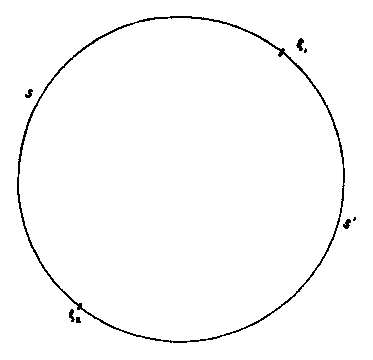
\includegraphics{chap04-vend-scan-01.eps}
\end{figure}

The foregoing discussion leads to the following result:


\begin{theorem*}
The part of the boundary of $R$ lying in $\mathscr{O}$ is the union of countably many pairs of conjugate sides\footnote{Possibly without their endpoints.} $(s_{i},\,s_{i}^{\prime})$ having the following properties:

\emph{1)} Each side is an are of an isometric circle or the full circle.

\emph{2)} To each side $s_{i}$ there is a side $s_{i}^{\prime}$ and a $V_{i}\in\Gamma$ such that $V_{i}s_{i} =s_{i}^{\prime}$. If $s_{i}$ and $s_{j}$ lie on different isometric circles, $V_{i}\neq V_{j}.$

\emph{3)} $s_{i}$ is not $\Gamma$-equivalent to a side different from $s_{i}^{\prime}$.

\emph{4)} $s_{i}$ and $s_{i}^{\prime}$ have equal euclidean length.
\end{theorem*}
That the number of sides is countable is clear, since each side is associated
with a different transformation of $\Gamma$ and there are only countably many transformations (\ref{ch03:chap03}. Th. \ref{ch03:sec1K}). Since $|dV_{i}/dz|=1$ on the circle $\Im(V_{i}), s_{i}$ is mapped onto $s_{i}^{\prime}$ without change of length. This completes the proof.

Nothing we have said precludes the possibility that $s =s^{\prime}$. If this is the case, $V$ must be elliptic with period 2, for the isometric circles of $V$ and $V^{-1}$ are disjoint or at most tangent when $V$ is not elliptic. In this case we shall regard the fixed points $\xi_{1},\,\xi_{2}$ of $V$ as points of category \textbf{a} 2 separating two equal sides, rather than as points of category \textbf{a} 1. Cf. Figure, p. 121.

The fundamental region may not possess any sides at all, that is, the entire boundary of $R$ may consist of points of category \textbf{b}. Cf. [\citeauthor{Ford0000}~\ref{Ford1}, p. 58].

\subsection{}\label{ch04:sec3C} Let us turn to points of category \textbf{a} 2. An ordinary\index{vertex!ordinary} point $\alpha$ can lie on only a finite number of isometric circles $\Im_{j},\,j=1,2,\cdots,\,t$. Let $C$ be a circle about $\alpha$ so small that it meets no isometric circle not in $\{\Im_{j}\}$ and contains no point of intersection of the $\{\Im_{j}\}$ except $\alpha$. The interior of $C$ is partitioned by the $\{\Im_{j}\}$ into a finite number of regions. At least one of the regions, say $\Delta$, meets $R$, since $\alpha$ is a boundary point of $R$. Then all of $\Delta$ belongs to $R$, for $R$ is bounded by isometric circles.

There are now several possibilities, which are illustrated in the Figures. The region $\Delta$ may be bounded by two \emph{different} isometric circles, $\Im_{1}$ and $\Im_{2}$, which may cut at a nonzero angle or may be externall{\.y} tangent. In the latter case $\Im_{1}$ and $\Im_{2}$ may be the boundary of two portions of $R$ or of only one. Finally, all circles through $\alpha$ except $\Im_{1}$, say, may be internally tangent to $\Im_{1}$ at $\alpha$; in this case $R$ is bounded at $\alpha$ by \emph{one} isometric circle, $\Im_{1}$.

Suppose $R$ is bounded by $\Im_{1}$ and $\Im_{2}$. Except for $\alpha$, the points of these two circles lying within $C$ are clearly points of category \textbf{a} 1, and the parts of $\Im_{1},\,\Im_{2}$ within $C$ are parts of sides of $R$. The same statement is true if $R$ is bounded by $\Im_{1}$ alone.

We call a point of category \textbf{a} 2, such as $\alpha$, an \emph{ordinary vertex}. The special case in which $\alpha$ lies on a single isometric circle of an elliptic substitution of period 2 has been mentioned (3B).

It is not hard to see that $V\alpha$ \emph{is an ordinary vertex if} $\alpha$ \emph{is an ordinary vertex lying on} $\Im(V)$. As before, $V\alpha$ is interior to no isometric circle. Let $\Im(W)$ be another isometric circle on which $\alpha$ lies. Then
\begin{equation*}
\delta(WV^{-1},\,V\alpha)=\delta(W,\,\alpha)\delta(V^{-1},\,V\alpha)=\delta^{-1}(V,\, \alpha)=1,
\end{equation*}
showing that $V\alpha$ lies on $\Im(WV^{-1})$. Since this is true for each isometric circle passing through $\alpha$ and we already know $V\alpha$ lies on $\Im(V^{-1})$, it follows that $V\alpha$ is on at least as many isometric circles as $\alpha$. But we can reverse the reasoning, starting with $V\alpha$ instead of $\alpha$, whence $\alpha$ and $V\alpha$ lie on the same number of isometric circles. Hence $V\alpha$ is an ordinary vertex. At least one of the isometric circles through $V\alpha$ bounds a portion of $R$.

We now wish to prove that \emph{if the image of a vertex} $\alpha$
\emph{lies on the boundary of} $R$ \emph{it is also a vertex}. This
is now practically evident. For if $\Im(T)$ does not pass through
$\alpha$, then $\alpha$ must be exterior to it and so $T\alpha$ lies
inside $\Im(T^{-1})$ and therefore outside $R$. Hence if $T\alpha$
lies on Bd $R,\,\Im(T)$ must pass through $\alpha$ and we have just
seen that $T\alpha$ is then an ordinary vertex.

\begin{figure}[!h]
\includegraphics{chap04-vend-scan-02.eps}
\end{figure}

The images of $R$ under the transformations of $\Gamma$ are fundamental regions
bounded by circular arcs,\footnote{In general, not arcs of isometric circles.} and we may assign to their boundaries the same names as we did to the boundary of \emph{R. By the sides and vertices of a region} $VR$ \emph{we mean the images under $V$ of the sides and vertices of} $R$. The set of all sides of the network of regions $\Gamma R$ is invariant under any $V\in\Gamma$; likewise the set of all ordinary vertices.

Let us now see how the fundamental regions are assembled about an ordinary vertex $\alpha$ of $R$. The immediate neighborhood of $\alpha$, being relatively compact, is covered by a finite number of images of $R$, say $R,\,V_{1}R,\cdots,V_{t}R$. The region $V_{1}R$ surely has $\alpha$ as a boundary point. Let $V_{1}^{-1}\alpha=\beta$; $\beta$ lies on Bd $R$ and is a vertex of $R$, for it is the image of a vertex of $R$. Hence by definition $\alpha$ is a vertex of $V_{1}R$. Each fundamental region having $\alpha$ on its boundary has $\alpha$ as a vertex.

\begin{figure}[!h]
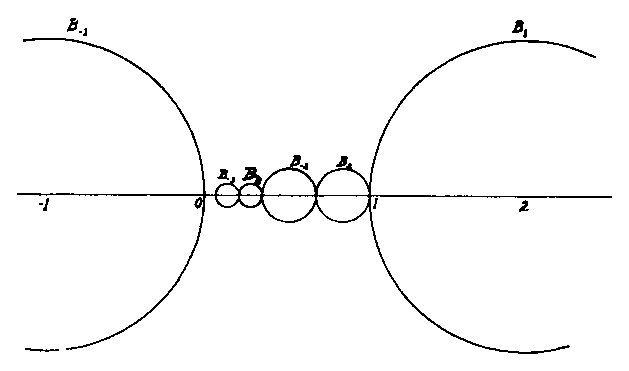
\includegraphics{chap04-vend-scan-03.eps}
\end{figure}

To summarize:


\begin{theorem*} $R$ is bounded at an ordinary vertex $\alpha$ by two isometric circles that meet at $\alpha$ or by one isometric circle that passes through $\alpha$. An image of $\alpha$ that lies on $\mathrm{Bd}$ $R$ is also an ordinary vertex. The immediate neighborhood of $\alpha$ is made up of a finite number of images of $R$ each of which has $\alpha$ as a vertex.
\end{theorem*}

\subsection{}\label{ch04:sec3D} We now take up category \textbf{b.} As far as points of category\index{point of category b3} \textbf{b} 1 are concerned, about all we can say is that such points exist. Consider the following system of circles (cf. Figure):
\begin{equation*}
B_{1}:\,|z-2|=1,\qquad B_{\mbox{-}1}:\,|z+1|=1,
\end{equation*}\index{point of category b1}

$B_{i},\,B_{-i},\,i=2, 3, 4,\cdots:$ two circles of equal radius, centers on real axis, tangent externally. $B_{2}$ is tangent externally to $B_{1},\,B_{i+1}$ is tangent externally to $B_{-i},\,i\geqq 2$. All $B_{i}(i\geqq 1)$ lie in the right half-plane. Finally $B_{i} \rightarrow 0,\, i\rightarrow\infty$. We see at once that the region exterior to $B_{i}\bigcup B_{-i}$ is a fundamental region for the group $G_{i}=\{T_{i}\}$, where $T_{i},\,T_{i}^{-1}$ are transformations having isometric circles $B_{i},\,B_{-i}$, respectively.

The conditions of Theorem 2B are fulfilled, and the free product of all $G_{i}$ is discontinuous. The origin is a limit point of $\Gamma$ since it is an accumulation point of the centers of the circles $\{B_{i}\}$; it lies on $B_{-1}$ and on no other isometric circle.

The reader will have no difficulty in modifying the above example so as to make the origin a point of category \textbf{b} 3.

Points of class \textbf{b} 2 will be treated in the next Section.


\section{Cycles}\label{ch04:sec4}

\subsection{}\label{ch04:sec4A} The relation of $\Gamma$-equivalence partitions the set of ordinary\index{cycle!ordinary} vertices of $R$ into disjoint equivalence classes called \emph{ordinary cycles}.


\begin{definition*} An ordinary cycle of $R$ is a set $\mathbf{C}$ of ordinary vertices of $R$ such that

1) any two elements of $\mathbf{C}$ are equivalent,

2) any vertex in $R$ equivalent to \textbf{a} vertex in $\mathbf{C}$ is in $\mathbf{C}$.
\end{definition*}

\begin{theorem*}
An ordinary cycle contains only a finite number of vertices.
\end{theorem*}

Let $\mathbf{C}=\{z_{1},\,z_{2},\cdots\}$. Let $z_{1}=T_{j}z_{j},\,j=1$, 2, $\cdots\,$. $T_{j}$ carries $R$ into a fundamental region $R_{j}$ with a vertex at $z_{j}$. If $\mathbf{C}$ is infinite, there are infinitely many fundamental regions meeting at $z_{1}$, and these regions are, of course, disjoint. A compact neighborhood of $z_{1}$ requires infinitely many images of $R$ to cover it, which is impossible (\ref{ch04:sec1F}). Hence the assertion.

\subsection{}\label{ch04:sec4B} If one vertex in $\mathbf{C}$ is a fixed point of an element of $\Gamma$, the same is true of every vertex, for $TET^{-1}$ fixes $Tz$ if $E$ fixes $z$. Furthermore, the transformation fixing an ordinary point is necessarily elliptic\index{cycle!elliptic}, for every neighborhood of a nonelliptic fixed point contains infinitely many equivalent points. We therefore classify an ordinary cycle as \emph{elliptic} or \emph{accidental}\index{cycle!accidental}, according as all or none of its vertices are fixed points. The order of the elliptic transformation which fixes a given point of the cycle is the same at each point of the cycle, for $E^{l}=I$ is synonymous with $(TET^{-1})^{l}=I$. This integer is called the \emph{order} of the elliptic cycle.

The sides of $R$ which meet at a vertex $v$ are circular arcs and form two angles at $v$. The measure of that angle which bounds a portion of $R$ will be termed the \emph{angle} at $v$ \emph{in} $R$. In the special case that the sides are tangent at $v$ there may be two such angles (both equal to $0$) and these angles are considered to be distinct. Or, what amounts to the same thing, $v$ is replaced by two vertices, each with its own angle in $R$. If $R$ is bounded at $v$ by a single arc, the angle is $\pi$ (cf.~\ref{ch04:sec3C}).


\subsection{}\label{ch04:sec4C} \begin{theorem*} The sum of the angles at the vertices of an ordinary cycle of $R$ is $2\pi/l$ if the cycle is elliptic of order l, and is $2\pi$ if the cycle is accidental. Conversely, if the angle sum\index{cycle!angle sum of} at the vertices of an ordinary cycle of $R$ is $2\pi/l$, the cycle is elliptic of order $l$ when $l>1$ and is accidental when $l=1.$
\end{theorem*}


Let $\mathbf{C}=\{z_{1},z_{2},\cdots, z_{s}\}$ be an elliptic cycle of order $l\geqq 2$, let $E$ be an elliptic substitution generating the isotropy subgroup\footnote{This is the subgroup of $\Gamma$ fixing $z_{1}$ and is cyclic. Cf. Note 5, p. 400.} $\Gamma_{z_{1}}$, and let $T_{j}\in\Gamma$ be fixed transformations such that $T_{j}z_{j}=z_{1},j=1,2,\cdots,\,s$. ($T_{j}$ is not unique.) The elements of $\Gamma$ which map $z_{j}$ on $z_{1}$ are precisely the transformations
\begin{equation*}
\mathbf{A}_{j}=\{E^{k}T_{j}|0\leqq k<l\},\qquad j=1,\cdots,s.
\end{equation*}
Indeed, from $Vz_{j}=z_{1}$ we deduce that $VT_{j}^{-1}$ fixes $z_{1}$ and so is a power of $E$, in other words $V\in \mathbf{A}_{j}$. On the other hand, each member of $\mathbf{A}_{j}$ obviously performs the required mapping, whence our assertion.

Secondly, the immediate neighborhood of $z_{1}$ is completely covered by the closures of fundamental regions. Let $R_{1}$ be such region and let $W(R)=R_{1},\, W\in\Gamma$. $R_{1}$ necessarily has $z_{1}$ as a vertex (Th. \ref{ch03:sec3C}). Hence $W$ must carry some vertex of $R$ into $z_{1}$. This vertex can only be a member of $\mathbf{C}$, say $z_{j}$. Then $W\in \mathbf{A}_{j}$. Conversely, every $W$ in $\mathbf{A}_{j}$ maps $R$ onto a fundamental region which has a vertex at $z_{1}$. The neighborhood of $z_{1}$ is made up of the closures of $sl$ fundamental regions, the images of $R$ by the transformations of $\{\mathbf{A}_{j},j=\,1,\,\cdots,\,s\}$.

Denote by $\theta_{j}$ the angle at $z_{j}$ in $R$. The angle $\theta_{kj}$, defined as the angle at $z_{1}$ in the fundamental region
\begin{equation*}
R_{kj}=E^{k}T_{j}(R),\quad k=0,\,1,\,\cdots,\,l-1
\end{equation*}
is equal to $\theta_{j}$ because of the conformality of the transformations of $\Gamma$. Hence
\begin{equation*}
2\pi=\sum\limits_{j=1}^{s}\sum\limits_{k=0}^{l-1}\theta_{kj}=l\sum\limits_{J=1}^{s}\theta_{j},
\end{equation*}
as promised in the statement of the theorem. The situation is illustrated in Figure~\ref{fig4.1}, p. 127 for the case $s=2,\,l=3$.

If $\mathbf{C}$ is an accidental cycle, the reasoning is similar. There are $s$ fundamental regions providing the neighborhood of $z_{1}$, namely, $T_{j}R,\,1\leqq j\leqq s$. (This time $T_{j}$ is unique, since $z_{1}$ is not a fixed point.) The angle at $z_{1}$ in $T_{j}R$ is equal to the angle at $z_{j}$ in $R$, and the result follows. We have proved the direct part of the theorem.

The converse follows by elementary reasoning. Thus if $\mathbf{C}$ is a cycle with angle sum $2\pi/l,\,l>1$, then, by what we have just proved, $\mathbf{C}$ cannot be elliptic of order $m\neq l$ nor can it be accidental. If the angle sum is $2\pi,\,\mathbf{C}$ cannot be elliptic of any order and so must be accidental. The theorem is proved.

\textit{Note.} Consider the application of this theorem to the fundamental
region shown in Figure.~\ref{fig4.2} The group is generated by two
hyperbolic transformations, one of which conjugates the large
circles, the other conjugates the small circles. According to the
convention of~\ref{ch04:sec4B}, the point of tangency must be
counted as \emph{two} vertices, $z_{1}$ and $z_{2}$. The points
$z_{1},\,z_{2}.\, z_{3},\,z_{4}$ comprise an accidental cycle. The angles at $z_{1}$ and $z_{3}$ are both zero, at $z_{2}$ and $z_{4}$ both $\pi$.

\begin{figure}[!h]
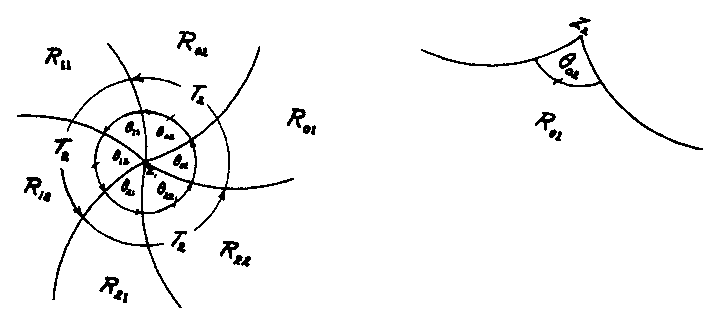
\includegraphics{chap04-vend-scan-04.eps}
\caption{}\label{fig4.1}
\end{figure}

\begin{figure}[!h]
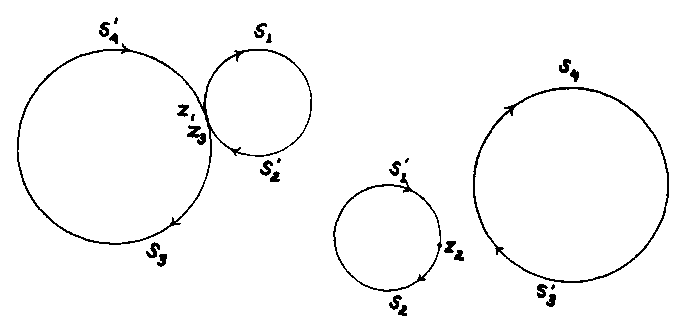
\includegraphics{chap04-vend-scan-05.eps}
\caption{}\label{fig4.2}
\end{figure}

\subsection{}\label{ch04:sec4D} Let $\alpha$ be an elliptic fixed point\index{point of category b2} of order $l$, and $K$ the interior of a fixed circle of $E$, the generator of $\Gamma_{\alpha}$. The regions $E^{k}T_{j}R,\,k=0, 1,\cdots,l-1$, are equally spaced around $\alpha$, each being obtained from the preceding one by a rotation through the angle $2\pi/l$. We can select $k=k_{j}$ depending on $T_{j}$ in such a way that the regions $\{E^{k_{j}}/T_{j}R,j=1,\,2,\,\cdots,\,s\}$ are \emph{adjacent}. We call
\begin{equation*}
\mathscr{S}_{\alpha}=\bigg\{\bigcup_{j=1}^{s}E^{k_{j}}T_{j}\bar{R}\bigg\}\cap\,K
\end{equation*}
an \emph{elliptic sector}\index{elliptic sector} at $\alpha$; it subtends an angle of $2\pi/l$.


\subsection{}\label{ch04:sec4E} By definition every elliptic\index{cycle!elliptic} cycle is made up of fixed points of elliptic elements. Is it true, conversely, that every elliptic fixed point is found in some elliptic cycle?

Let $\alpha$ be an \emph{ordinary} point fixed by an elliptic transformation $E$ of period $l$. Application of $E$ amounts to a (noneuclidean) rotation about $\alpha$ through an angle $2\pi/l$. Now $\alpha$ is found in the closure of some fundamental region $R_{1}$, an image of $R$. Clearly $\alpha$ is no interior point of $R_{1}$, for a sufficiently small neighborhood would lie in $R_{1}$ and contain $l$ points equivalent under $E$. Suppose $\alpha$ is an inner point of a side $s$ of $R_{1}$. If $l>2$, we can still find two equivalent points on the same side of $s$ and therefore in $R_{1}$. If $l=2$, the isometric circle on which $s$ lies is mapped into itself by $E;\alpha$ divides $s$ into two equal segments. Under these circumstances we have agreed to call $\alpha$ a vertex ( 3B). We have proved:


\begin{theorem*}
Every elliptic fixed point which is an ordinary point is a point of an elliptic cycle.
\end{theorem*}

\subsection{}\label{ch04:sec4F} Consider now points of category \textbf{b} 2 (cf.~\ref{ch04:sec3A}). As a first case let $p$, a limit point of $\Gamma$, be a boundary point of $R$ where two isometric circles meet, and let there be no point of $\bar{R}$ equivalent to $p$. Suppose $s$ is a side of $R$ having the endpoint $p$. Then $s^{\prime}=Ps$, the conjugate of $s$, also has the endpoint $p$, otherwise $p$ would have an equivalent point in $R$, namely, one of the endpoints of \emph{Ps}. By the same token $Pp=p$.

The fixed points of hyperbolic and loxodromic substitutions lie within their isometric circles (\ref{ch02:chap02}.~\ref{ch02:sec10B}): hence $P$ is elliptic or parabolic. In the first case $s$ and $s^{\prime}$ make an angle of $2\pi/l$ for some integer $l>1$. Then $l$ images of $R$ are sufficient to cover the complete neighborhood of $p$. This is a contradiction, for $p$ is a limit point (\ref{ch04:sec1G}).

Hence $P$ is parabolic, and this implies that $s$ and $s^{\prime}$ are tangent. The powers of $P$ map $R$ into fundamental regions whose sides pass through $p$ and are tangent to $s$. The angle at $p$ in each fundamental region is zero. If $K$ is the interior of a fixed circle of $P$, then
\begin{equation*}
K=\bigcup_{q=-\infty}^{\infty}P^{q}(K\cap\bar{R}).
\end{equation*}


\subsection{}\label{ch04:sec4G} The situation when $p$ has equivalent points on the boundary of $R$ is somewhat more complicated. Let $\{p_{1},\,p_{2},\,\cdots\}$ be the complete set of points of $R$ (necessarily boundary points) equivalent to $p_{1}=p$. We expressly assume each $p_{i}$ lies on two sides of $R$. If we think of the boundary of $R$ described in the positive sense, each side will have an initial point and a terminal point. When a side $s$ is mapped onto its conjugate side $s^{\prime}$ by $V$, the initial (terminal) point of $s$ goes into the terminal (initial) point of $s^{\prime}$, because $V$ interchanges the interior and exterior of $\Im(V)$ and $\Im(V^{-1})$.

Suppose $s_{1}$ is a side beginning at $p_{1}$. The conjugate of $s_{1}$ is a side $s_{1}^{\prime}$ ending at $p_{2}$ (cf. Figure). There is a side $s_{2}$ beginning at $p_{2}$ whose conjugate side $s_{2}^{\prime}$ ends at $p_{3}$, and so on.

It may happen that after $t$ steps the conjugate side
$s_{t}^{\prime}$ ends at $p_{1}$. The Figure illustrates this case
for $t=3$. \emph{Then we say that the set}
$\{p_{1},\,p_{2},\,\cdots,\,p_{t}\}$ \emph{is a parabolic cycle of}\index{cycle!parabolic}\index{vertex!parabolic}
$R$. Cf. Note 5a, p. 400.

\begin{figure}[!h]
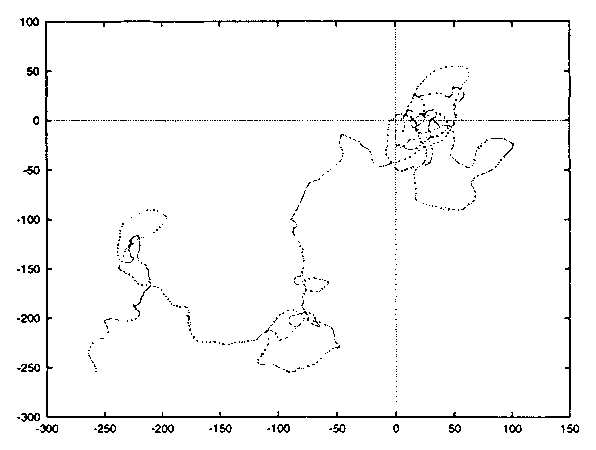
\includegraphics{chap04-vend-scan-06.eps}
\end{figure}

Let $W_{j}$ be an element of $\Gamma$ such that
\begin{equation*}
W_{j}p_{j}=p_{j+1},\quad j=1,2,\,\cdots,\,t-1;\qquad W_{t}p_{t}=p_{1}.
\end{equation*}
The transformation
\begin{equation}
\label{ch04:eqn6}
P=W_{t}W_{t-1}\cdots W_{2}W_{1}
\end{equation}
maps $p_{1}$ on itself and so is either elliptic or parabolic.

In order to exclude the first possibility, we consider the arrangement of those fundamental regions which have a vertex at $p_{1}$. Now $W_{t}$ carries $p_{t}$ into $p_{1}$ and carries $R$ into a fundamental region $R_{t}$ having a vertex at $p_{1}$. Since $W_{t}$ maps $s_{t}$ on $s_{t}^{\prime}$, it is seen that $R_{t}$ must have the side $s_{t}^{\prime}$ in common with $R$; hence $R,\,R_{t}$ are in counterclockwise order around $p_{1}$. Let $s_{t-1}^{\ast}$ be the other side of $R_{t}$ issuing from $p_{1}:W_{t}s_{t-1}^{\prime}=s_{t-1}^{\ast}$. Next, $W_{t}W_{t-1}$ carries $p_{t-1}$ to $p_{1}$ and carries $R$ to a fundamental region $R_{t-1}$ with vertex at $p_{1}$. Since $W_{t}W_{t-1}s_{t-1}=W_{t}s_{t-1}^{\prime}=s_{t-1}^{\ast}$, it is clear that $R_{t-1}$ abuts $R_{t}$ along $s_{t-1}^{\ast}$ and $R_{t},\,R_{t-1}$ are in counterclockwise order around $p_{1}$. (Cf. Figure.) Continuing in this way, we obtain the regions $R,\,R_{t},\, R_{t-1},\cdots,\,R_{1}$ in counterclockwise order around $p_{1};R_{1}$ is the image of $R$ by $P$.

We now see that $P$ connects two sides $s_{1}$ and $s^{\ast}$ issuing from $p_{1}$, and these two sides include a block of $t$ fundamental regions $R,\,R_{t},\,R_{t-1},\,\cdots,\,R_{2}$. The

\begin{figure}[!h]
\includegraphics{chap04-vend-scan-07.eps}
\end{figure}

\noindent reasoning of~\ref{ch04:sec4F} can now be used to show that $P$ is parabolic. The sides of $R$ which meet at $p_{1}$ and indeed at $p_{j},\,1\leqq j\leqq t$, are tangent.

Let $\Gamma_{p}^{\ast}$\index{$\Gamma_{p}^{\ast}$} be the set of all \emph{parabolic} elements of $\Gamma$ which fix $p$, where we have written $p$ for $p_{1}$. It is at once verified that $\Gamma_{p}^{\ast}$ is a subgroup of $\Gamma$. We are going to show that $\Gamma_{p}^{\ast}$ is \emph{cyclic and is generated by} $P$.

According to~\ref{ch03:chap03}.~\ref{ch03:sec2B}, $\Gamma_{p}^{\ast}$ is either cyclic or has two generators. Suppose the latter: $\Gamma_{p}^{\ast}=\{P_{1},\,P_{2}\}$,
\begin{equation*}
P_{j}=\left(\begin{matrix}
1+c_{j}p & -c_{j}p^{2}\\c_{j} & 1-c_{j}p
\end{matrix}\right),\quad j=1,2.
\end{equation*}
Also
\begin{equation*}
\Im(P_{j}):\bigg|z-\bigg(p-\frac{1}{c_{j}}\bigg)\bigg|=\frac{1}{|c_{j}|},\quad\Im(P_{j}^{-1}):\bigg|z-\bigg(p+\frac{1}{c_{j}}\bigg)\bigg|=\frac{1}{|c_{j}|},\quad
j=1,2.
\end{equation*}

Suppose $c_{1}/c_{2}$ is not real. Then the region exterior to these 4 isometric circles does not contain $p$ as an interior or boundary point. Hence $p\not\in \bar{R}$, a contradiction.

We must therefore assume $c_{1}/c_{2}$ real. Let $A=(0,\,-1\big|1,\,-p)$. We calculate
\begin{equation*}
AP_{j}A^{-1}=\left(\begin{matrix}
1 & -c_{j}\\0 & 1
\end{matrix}\right),\qquad AP_{1}^{m}P_{2}^{n}A^{-1}=\left(\begin{matrix}
1 & -mc_{1}-nc_{2}\\0 & 1
\end{matrix}\right),
\end{equation*}
both elements of the discontinuous group $A\Gamma_{p}^{\ast}A^{-1}$. The module $\{mc_{1}+nc_{2}\big|m,\,n=\mathrm{integer}\}$, which consists of points all lying on one line, is discrete, otherwise $A\Gamma A^{-1}$ would not be discrete. Hence (\ref{ch02:chap02}. \ref{ch02:sec13A}) there is a $c_{0}=m_{0}c_{1} +n_{0}c_{2}$ which generates the module, i.e., $A\Gamma_{p}^{\ast}A^{-1}= \{AP_{0}A^{-1}\}$, where $P_{0}=(1+c_{0}p, -c_{0}p^{2}|c_{0},1-c_{0}p)$. Hence $P_{0}$ generates $\Gamma_{p}^{\ast}$.

Finally we shall show that the transformation $P$ of (6) is either $P_{0}$ or $P_{0}^{-1}$ and \emph{s}o generates $\Gamma_{p}^{\ast}$. For this purpose we recall the arrangement of the fundamental regions about $p$ which we discussed earlier: the regions $R,\,R_{t},\,R_{t-1},\,\cdots,\,R_{1}$ are adjacent and in counterclockwise order. $P$ maps a side $s$ of $R$ on a side $s^{\prime}$ of $R_{1}$. There is a fixed circle of $P$ passing through $p$ and cutting $s$ and $s^{\prime}$; if $K$ denotes its interior, the region
\begin{equation*}
\mathscr{T}_{p}=\bigg\{\bar{R}\bigcup_{i=2}^{t}\bar{R}_{i}\bigg\}\cap\,K
\end{equation*}
is called a \emph{parabolic sector} at $p$. $P$ maps a parabolic sector on another parabolic sector, and
\begin{equation}
\label{ch04:eqn7}
K=\bigcup_{q=-\infty}^{\infty}P{^q}\mathscr{T}{_{p}}.
\end{equation}
We observe that $K-p$ lies entirely in $\mathscr{O}$ since $\mathscr{T}$ lies in $\mathscr{O}$.

Now consider $P_{0}$, the known generator of $\Gamma_{p}^{\ast}$; we wish to show that $P=P_{0}$ or $P_{0}^{-1}$. Since $P$ maps $R$ on $R_{1}$ we can find an integer $m$ such that $P^{m}P_{0}R =R_{j}$, for some $j$ in $1\leqq j\leqq t$. Then $P^{m}P_{0}=W_{t}W_{t-1}\cdots W_{j}$, since both members map $R$ on $R_{j}$. But $j>1$ is impossible, for in that case $W_{t}\cdots W_{j}$ is not even in $\Gamma_{p}^{\ast}$ since its inverse does not preserve $p$. Hence $j=1$ and $P^{m-1}P_{0}R=R$, so $P_{0}=P^{1-m}$. However, $P_{0}$ generates and this gives, with $1-m=q,\,P=P_{0}^{l}$,
\begin{equation*}
P_{0}=P^{q}=P_{0}^{lq}.
\end{equation*}
Thus $lq =1$ and $q=\pm 1$, as required.

We summarize in a


\begin{theorem*}
Each vertex $p_{i}$ of a parabolic cycle $(p_{1}, p_{2},\,\cdots,\, p_{t})$ of $R$ is the fixed point of a parabolic transformation $P_{i}$ of $\Gamma.$
$P_{i}$ generates the infinite cyclic subgroup $\Gamma_{pi}^{\ast}$ of those parabolic elements of $\Gamma$ which fix $p_{i}$. Each $p_{i}$ is the point of intersection of two sides of $R$. The angle at $p_{i}$ is zero in $R$ and in all images of $R$ having a cusp at $p_{i}$. $P_{i}$ maps the two sides of a parabolic sector at $p_{i}$ \emph{(}consisting of $t$ images of $R$\emph{)} on each other.
\end{theorem*}

\textit{Remark.} We call $K$ a horocycle\index{horocycle}. Horocycles are usually defined for a disk; they are simply euclidean circles which are tangent internally to the boundary of the disk. What we have shown is that there is a horocycle lying, except for one point, entirely in $\mathscr{O}$. This is quite remarkable when we consider how complicated the boundary of $\mathscr{O}$ is in case $\Gamma$ is not a principalcircle group (and has more than 2 limit points). For then $\Gamma$ contains loxodromic elements. There are infinitely many loxodromic fixed points, since

\begin{figure}[!h]
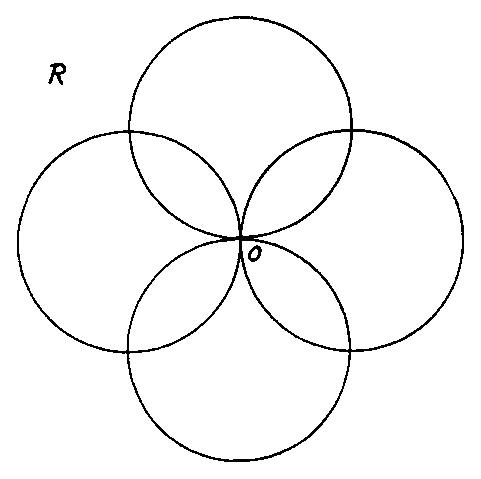
\includegraphics{chap04-vend-scan-08.eps}
\end{figure}

\noindent $TLT^{-1}$ is loxodromic if $L$ is and $T\in\Gamma$.
Suppose $\alpha$ and $\beta$ are two such fixed points not both
belonging to the same transformation. Then if $\alpha$ is fixed by
$L,\,(L^{m}\beta)$ is a sequence of points spiraling about $\alpha$.
But each $L^{m}\beta$ is itself a loxodromic fixed point and so has
spirals of other fixed points around it. Since the fixed points lie
everywhere dense among the limit points (\ref{ch03:chap03}. Th. \ref{ch03:sec4H}), the
complexity of the resulting configuration is readily apparent. For
examples cf. [\citeauthor{Fricke0000a}\index{Fricke-Klein} \ref{Fricke1a}, pp. 411--428];
[\citeauthor{Magnus0000}~\ref{Magnus1}\index{Magnus}, pp. 80--90].

The existence of horocycles in the general discontinuous group is a sort
of convexity property. It has apparently not yet been exploited.

\subsection{}\label{ch04:sec4H} Unfortunately the converse of the last theorem is untrue. There are groups containing parabolic\index{vertex!parabolic} transformations whose fixed points are not cusps of any fundamental region. The simplest example is the doubly periodic group. Here the fundamental region is a parallelogram, but the only fixed point of the group is at $\infty$, which does not appear as a vertex of any parallelogram. It may be objected that our theory does not apply, since $\infty$ is not an ordinary point. But we can transform the group so that $\infty$ is carried to $0$; the fundamental region is then the exterior of 4 isometric circles. (Cf. Figure, where the fundamental region for the group generated by $(1\,0\,|\,1\,1), (1\,0\,|\,i\,1)$ is pictured.)

We shall call the fixed point of a parabolic transformation a \emph{parabolic point}\index{parabolic point}, and shall reserve the name \emph{parabolic vertex} for the fixed point of a parabolic transformation lying on the boundary of $R$ or of one of its $\Gamma$-images.

The situation for principal-circle groups is more satisfactory. Cf. Theorem \ref{ch04:sec7E}.


\subsection{}\label{ch04:sec4I} If $\alpha$ is an ordinary point and the fixed point of an elliptic transformation, $\Gamma_{\alpha}$ is an elliptic cyclic group. We might hope that when $p$ is the fixed point of a parabolic transformation, $\Gamma_{p}$ is a parabolic cyclic group. This is not true in general, for \ref{ch03:chap03}. Th. \ref{ch03:sec2C} furnishes an example of a group in which $\infty$ is fixed by both parabolic and elliptic substitutions. This is why in Theorem 4G
we had to consider $\Gamma_{p}^{\ast}$ rather than $\Gamma_{p}$.

The situation cannot arise in principal-circle groups (Section~\ref{ch04:sec6}). An elliptic fixed point is interior to the principal circle, whereas a parabolic point\index{parabolic point} is on the principal circle.


\subsection{}\label{ch04:sec4J} The groups with fundamental regions\index{fundamental region!with infinite number of sides} bounded by a finite number of sides form an important class. Indeed, these are the groups whose associated Riemann surfaces are compact. Most of the theory has been developed for these groups only. The following theorem gives a sufficient condition for a group to be in this class.


\begin{theorem*}
$R$ has a finite number of sides provided the boundary points of $R$ are either ordinary points or parabolic vertices.
\end{theorem*}

Suppose $R$ has the sides $s_{1},\,s_{2},\,\cdots$. Let $z_{i}$ be a point of $s_{i}$ such that no two $z_{i}$ are equal. The set $\{z_{i}\}$ has an accumulation point $z^{\ast}$, and $z^{\ast}$ is clearly a boundary point of $R$. Every neighborhood of $z^{\ast}$ meets infinitely many sides of $R$, which is impossible: the immediate neighborhood of an ordinary point or parabolic vertex meets at most two sides of $R$.

\subsection{}\label{ch04:sec4K} A parabolic vertex is a boundary point of category\index{point of category b2} \textbf{b} 2. We obtained a parabolic cycle in~\ref{ch04:sec4G} by assuming that the process given there terminates, that is, after a finite number of steps we return to the first side. Two other possibilities can occur however:

1) The process does not terminate. That is, for no $k$ does $s_{k}^{\prime}$ end in $p_{1}$. We have then an infinite cycle $(p_{1}, p_{2},\cdots)$.

2) There is a $k$ such that $s_{k+1}$ does not exist, i.e., there is a side ending in $p_{k}$ but no side beginning in $p_{k}$.

Examples, similar to the one in~\ref{ch04:sec3D}, are easy to construct. The details are left to the reader.


\section{Function Groups}\label{ch04:sec5}\index{function group}

\subsection{}\label{ch04:sec5A} Let $\Gamma$ be a discontinuous group and let $\{\mathscr{D}_{i},\,i=1,2,\cdots\}$ be the regions of discontinuity of $\Gamma$ (\ref{ch03:chap03}.~\ref{ch03:sec5A}). We have already defined $\Gamma$ to be a \emph{function group}\index{fundamental region!of function group} provided one of the regions $\mathscr{D}_{j}$ is mapped on itself by each element of $\Gamma$ (\ref{ch03:chap03}.~\ref{ch03:sec5B}). $\mathscr{D}_{j}$ is called a domain of existence of $\Gamma$.

Let $\Gamma$ be a discontinuous function group with domain of existence $\mathscr{D}$. We still assume that $\infty$ (which may or may not lie in $\mathscr{D}$) is ordinary for $\Gamma$ and is not a fixed point. Each transformation of $\Gamma-I$ has an isometric circle. The set $R$, defined in~\ref{ch04:sec1D}, consisting of those points each of which is exterior to all isometric circles is a fundamental region for $\Gamma$ relative to $\mathscr{O}$. We obtain a fundamental region relative to $\mathscr{D}$ by merely intersecting $R$ with $\mathscr{D}$.


\begin{theorem*}
Define
\begin{equation*}
R_{0}=R\cap\,\mathscr{D}.
\end{equation*}
Then $R_{0}$ is a fundamental region for $\Gamma$ relative to $\mathscr{D}$. Every point of $\mathscr{D}$ is equivalent to a point of $\bar{R}_{0}$.
\end{theorem*}

Suppose $R$ does not meet $\mathscr{D}$. Each $z_{0}\in \mathscr{D}$ is equivalent to a point of $R$, hence equivalent to a point of $\sim \mathscr{D}$. Thus there is an element of $\Gamma$ which does not map $\mathscr{D}$ into itself, a contradiction. It follows that $R_{0}$ is not empty.

Since $R$ and $\mathscr{D}$ are open, the same is true of $R_{0}$. If $z\in R_{0}$, then $z\in R$ and $Vz$ is outside of $R$---hence outside of $R_{0}$---for each $V\in\Gamma-I$. Let $z\in$ Bd $R_{0}$. Then it is clear that $z\in \mathrm{Bd}\ R$. Let $N$ be a neighborhood of $z$ lying in $\mathscr{D}$. There is a point $x$ in $N-R$ (hence in $N-R_{0}$) equivalent to a point $y\in R$. But $y\in \mathscr{D}$, since $\Gamma$ preserves $\mathscr{D}$. Hence $y\in R_{0}$. The second requirement in the definition is satisfied and $R_{0}$ is a fundamental region. Each $z\in \mathscr{D}$ is equivalent to a point $w\in\bar{R}$, but $w$ is actually in $\mathscr{D}$ for the same reason as before. Hence $w\in\bar{R}_{0}$ and the proof is complete.

\emph{From now on we assume} $\Gamma$ \emph{is a function group}.

\subsection{}\label{ch04:sec5B} The fundamental region $R_{0}$ is bounded partly by sides (arcs of isometric circles). That is, unlike the general discontinuous group, a function group\index{fundamental region!of function group} cannot have a fundamental region bounded entirely by limit points (cf. end of \ref{ch02:sec3B}). If that were the case, $R_{0}$ would have no boundary points in $\mathscr{D}$, which implies $\mathscr{D}\ =R_{0}$ (cf. \ref{ch02:chap02}. Ex. 2-2). $\Gamma$ is an infinite group, otherwise there would be no limit points. No two distinct points of $\mathscr{D}$ are equivalent, a contradiction.


\subsection{}\label{ch04:sec5C} The theorems we have proved about $R$ carry over directly to $R_{0}$. For example, the part of the boundary of\index{fundamental region!boundary of} $R_{0}$ lying in $\mathscr{D}$ consists of a countable number of pairs of conjugate sides\index{conjugate side}. Suppose, in fact, that $s$ is a side\index{side} of $R$ which meets $\mathscr{D}$. Then $s$ must lie entirely in $\mathscr{D}$ except possibly for its endpoints. For if $s$ leaves $\mathscr{D}$ it must leave by a limit point $\lambda$ of $\Gamma$, since $\mathscr{D}$ is bounded entirely by limit points (\ref{ch03:chap03}.~\ref{ch03:sec5A}). Hence $\lambda$ is an endpoint of $s$ (cf. \ref{ch02:sec3B}). There is a unique element $V\in\Gamma,\,V\neq I$, such that $Vs=s^{\prime}$ is also a side of $R$. But $s^{\prime}$ lies in $\mathscr{D}$, for $V$ maps $\mathscr{D}$ on itself. Hence $s^{\prime}$ is a side of $R_{0}$.

In the same way we treat cycles. An ordinary\index{cycle!ordinary} cycle of $R_{0}$ is an equivalence class of ordinary vertices of $R_{0}$. A cycle in $R_{0}$ is clearly a cycle in $R$. Conversely, if one vertex of a cycle in $R$ lies in $R_{0}$, then all vertices lie in $R_{0}$. Thus Theorem \ref{ch04:sec4C} is valid for ordinary cycles of $R_{0}$. Similarly, Theorem \ref{ch04:sec4G} is valid for parabolic\index{cycle!parabolic} cycles of $R_{0}$.


\begin{theorem*}
Theorems\emph{~\ref{ch04:sec1F},~\ref{ch04:sec1G},~\ref{ch04:sec1H}, 3B,~\ref{ch04:sec4C},~\ref{ch04:sec4E},} and\emph{~\ref{ch04:sec4G}} are still true when we replace $R$ by $R_{0}$ in the statement of the theorem.
\end{theorem*}

\subsection{}\label{ch04:sec5D} In the simplest groups, such as the simply and doubly periodic groups, the modular group, etc., we notice that the transformations which pair the conjugate sides generate\index{function group!generation of} the group. We now prove this is true in general.


\begin{theorem*}
Let the sides of $R_{0}$ be denoted by $s_{n},\,s_{n}^{\prime},\,n=1,2,\cdots,$ and let $T_{n}\in\Gamma$ be such that $T_{n}s_{n}=s_{n}^{\prime}$. Then $\Gamma=\{T_{n}|n=1,2,\cdots\}$, that is, the transformations $\{T_{n}\}$ generate $\Gamma$.
\end{theorem*}

Set $\Theta=\{T_{n}|n=1,2,\cdots\}$. We have to show that $\Gamma \subset\Theta$.

Let $V$ be an arbitrary element of $\Gamma$ and let $V(R_{0})=R^{\ast}$. Choose $z_{0}\in R_{0}$ and $z_{1}\in R^{\ast}$. Join $z_{0}$ to $z_{1}$ by a curve $C$ which is bounded away from Bd $\mathscr{D}$. Then $C$ is compact and is covered by a finite number of fundamental regions (images of $R_{0}$). We can make small detours in $C$, if necessary, to insure that $C$ does not pass through a vertex. Let $R_{0},\, R_{1},\cdots,R_{n}=R^{\ast}$ be the regions crossed in turn as $C$ is described from $z_{0}$ to $z_{1}$. Let $V_{k}\in\Gamma$ map $R_{k}$ on $R_{k+1},\,k=0,1,\,\cdots,\,n-1$.

$V_{0}$ maps a certain side $s_{0}$ of $R_{0}$ on $s_{0}^{\prime}$, the side common to $R_{0}$ and $R_{1}$. Then $V_{0}$ is some $T_{i}\in\Theta$, say $T_{i_{0}}$.

Next, suppose $V_{1}$ maps $s_{1}$ (a side of $R_{1}$) onto $s_{1}^{\prime}$. The sides $T_{i_{0}}^{-1}s_{1}$ and $T_{i_{0}}^{-1}s^{\prime}_{1}$ are conjugate sides of $R_{0}$; let $T_{i_{1}}$ map the first on the second. Then clearly $V_{1}=T_{i_{0}}T_{i_{1}}T_{i_{0}}^{-1}$, for both transformations map $s_{1}$ on $s_{1}^{\prime}$. Hence $V_{1}\in\Theta$.

Suppose we have shown that $V_{0},\,V_{1},\,\cdots,\,V_{k-1}$ are in $\Theta$. Write $W= V_{k-1}V_{k-2}\cdots V_{1}V_{0}$; note that $W$ is in $\Theta$ and maps $R_{0}$ on $R_{k}$. Let $V_{k}$ map $s_{k}$ (a side of $R_{k})$ on $s_{k}^{\prime}$. The sides $W^{-1}s_{k},\,W^{-1}s_{k}^{\prime}$ are conjugate sides in $R_{0}$; therefore there is a $T^{\ast}\in\Theta$ such that $T^{\ast}W^{-1}s_{k}=W^{-1}s_{k}^{\prime}$. Now $V_{k}= WT^{\ast}W^{-1}$, for both transformations have the same effect on $s_{k}$. Hence $V_{k}\in\Theta$ and the induction is complete: all $V_{i},\,i=0,1,\cdots,\,n-1$, belong to $\Theta$. But $V_{n-1}V_{n-2}\cdots V_{1}V_{0}$ maps $R_{0}$ on $R_{n}$ and so this transformation must be identical with $V$; it follows that $V\in\Theta$. Since $V$ was any element of $\Gamma$, the theorem is proved.

No claim is made that $\{T_{n}\}$ is a minimal set in any sense.

\textit{Remark.} The theorem is true and the proof valid if $R_{0}$ is replaced by any fundamental region bounded by a countable number of Jordan arcs which are conjugate in pairs by elements of $\Gamma$.

\subsection{}\label{ch04:sec5E} Let $\alpha$ be an ordinary vertex. Enclose $\alpha$ in a small circle which contains no other vertex. Let $S_{1},\,S_{2},\,\cdots,\,S_{t}$ be the fundamental regions which have $\alpha$ as a vertex, listed in counterclockwise order. If we write $T_{i}S_{i}=S_{i+1},\,i=1,\,2,\cdots,\,t-1$, and $T_{t}S_{t}=S_{1}$, we have
\begin{equation*}
T_{t}T_{t-1}\cdots T_{2}T_{1}=I,
\end{equation*}
for the left member maps $S_{1}$ on itself. This equation is called a \emph{relation in}\index{function group!relations in a} $\Gamma$.

It is clear that every ordinary vertex gives rise to a relation, but it is not evident that these relations are independent, that is, that some relations are not consequences of others. We shall see later (\ref{ch07:chap07}. Th. \ref{ch07:sec2F}) that the above ``method of loops,'' due to Poincar\'{e}\index{Poincar\'{e}}, does produce a basis for the complete set of relations in a wide class of groups.

Let $\alpha_{1}$ be an ordinary vertex. In the early paragraphs of~\ref{ch04:sec4G} we gave a method for finding the remaining vertices $\alpha_{2},\,\alpha_{3},\,\cdots,\,\alpha_{t}$ of the cycle determined by $\alpha_{1}$. (The method was stated for parabolic cycles but applies equally well to ordinary cycles.) As before we denote by $W_{j}$ the element of $\Gamma$ such that $W_{j}s_{j}=s_{j}^{\prime},\,s_{j}$, being the side beginning at $\alpha_{j}$. Then $W_{t}W_{t-1}\cdots W_{1}=I$ for an accidental cycle and $(W_{t}W_{t-1}\cdots W_{1})^{l}=I$ for an elliptic cycle of order $l$, as we deduce easily from the discussion in~\ref{ch04:sec4G}. The two cases correspond to $R_{1}=R,\,R_{1}\neq R$, respectively.


\subsection{}\label{ch04:sec5F} For some purposes it is necessary to have a \emph{connected}\index{fundamental region!connected} fundamental region, and it is always convenient. Whether $R_{0}$, the standard fundamental region, is always connected I do not know; I can neither prove this result nor produce a counterexample. However, in certain cases it is possible to modify $R_{0}$ so as to make it connected.


\begin{theorem*}
If $R_{0}$ is bounded by a finite number of sides, there exists a fundamental region of $\Gamma$ which is a connected set and is bounded by circular arcs.
\end{theorem*}

Let $P_{1},\,P_{2},\cdots,P_{t}$ be the connected components of $R_{0}$. The components are open sets (\ref{ch02:chap02}.~\ref{ch02:sec2I}). Their number is finite since $R_{0}$ has a finite number of sides. From the formula (\ref{ch02:chap02}. Ex. 2-1)
\begin{equation*}
\mathrm{Bd}\ R_{0}\supset\bigcup_{i=1}^{t} \mathrm{Bd}\ P_{i},
\end{equation*}
we deduce that each $P_{i}$ is bounded by arcs of isometric circles, i.e., by sides. For a point on the boundary of $P_{i}$ lies on the boundary of $R_{0}$ and therefore lies on a side of $R_{0}$ (cf.~\ref{ch04:sec5C}).

Consider the sides of $P_{1}$. Each side is equivalent under $\Gamma$ to a unique side of one of the regions $P_{i}$. If every side of $P_{1}$ is equivalent to a side of $P_{1}$, we leave $P_{1}$ alone except to change its name to $Q$. The process ends at this point. If, on the contrary, a side $s_{1}$ of $P_{1}$ is equivalent by $T\in\Gamma$ to a side $s_{2}$ of $P_{i}$, we eliminate $P_{1}$ and replace $P_{i}$ by $P_{i}\cup TP_{1}\cup s_{2}^{\ast}$, where $s_{2}^{\ast}$ is $s_{2}$ without its endpoints. The set replacing $P_{i}$, which is still called $P_{i}$, is a region bounded by circular arcs and no two distinct points of the region are equivalent.

If $P_{1}$ has been adjoined to a $P_{i}$, consider $P_{2}$. In case each side of $P_{2}$ is equivalent to some other side, we label it $Q$ and stop; otherwise we adjoin it to a $P_{j}$ and proceed to $P_{3}$. We can continue the process until we get a region bounded entirely by pairs of conjugate arcs or until all $P_{i}$ have been combined in a single region. This last region is then seen to have the same property. At no stage of the process can there be overlapping of regions, for all $P_{i}$ are components of one fundamental region $R_{0}$. The set $Q$ obtained in this way after a finite number of steps is an open, connected set whose boundary consists of finitely many pairs of circular arcs, the two arcs of a pair being equivalent a transformation of $\Gamma$.

We assert $Q$ is a fundamental region. Indeed, if $x,\,y$ are distinct equivalent points of $Q$, then for suitable $V,W\in \Gamma,\,Vx$ and $Wy$ are in some $\bar{P}_{i}$ and $\bar{P}_{j}$ respectively, and hence in $\bar{R}_{0}$. If $Vx$ is an inner point of $R_{0},\,x$ and $y$ cannot be equivalent. Suppose $Vx\in \mathrm{Bd}\,P_{i},\,Wy\in \mathrm{Bd}\,P_{j}$. The case $i=j$ is trivial; $Vx$ and $Wy$ are then points lying on the same or equivalent sides of a single $P_{i}$. In the second case the sides remain in the boundary of $Q$ and $x,\,y$ are not in $Q$, which is an open set. In the first case $Vx$ and $Wy$ can only be endpoints of the side on which they both lie; hence $x,\,y$ are again boundary points of $Q$.

We may therefore assume $i<j$. Then $P_{i}$ must have been joined to some other polygon in the process described above, otherwise $P_{i}=Q$ and $y\not\in Q$. In fact, $P_{i}$ must have been joined to $P_{j}$ if we assume $x$ and $y$ are inner points of their respective sides, for the side containing $x$ is equivalent to exactly one side of $R_{0}$. In the joining, the equivalent points $Vx$ and $Wy$ are made to coincide and $x=y$, a contradiction. Thus $Vx,\,Wy$ must be vertices. But in the joining process a side of a polygon either disappears or becomes a side of $Q$, and in any event vertices remain vertices. In every case we have obtained a contradiction and we conclude that $Q$ contains no distinct equivalent points.

Suppose $\alpha$ is a boundary point and $\alpha^{\prime}$ an equivalent point on another side of $Q$; let $N$ be a neighborhood of $\alpha$ and $N^{\prime}$ the equivalent neighborhood of $\alpha^{\prime}.$ Now no point of $Q\cap N$ can be equivalent to an $x^{\prime}$ in $Q\cap N^{\prime}$, for both points lie in $Q$. Hence the point $x$ of $N$ equivalent to $x^{\prime}$ must lie outside $Q$. That is, there are points near $\alpha$ not in $Q$ equivalent to points of $Q$. Secondly, suppose $\alpha$ is not equivalent to any other point of $\mathrm{Bd}\,Q$; then $\alpha$ must be an elliptic fixed point constituting a cycle. Hence there is an element of $\Gamma$ conjugating the two sides issuing from $\alpha$ and the desired conclusion follows easily. Finally if $\alpha$ is a limit point, there are points in every neighborhood of $\alpha$ equivalent to any given point of $Q$ (cf. \ref{ch03:chap03}. Th. \ref{ch03:sec4A}), and such points of course lie in the complement of $Q$.

We have shown $Q$ satisfies the two requirements of a fundamental region and have remarked that it is bounded by circular arcs. The theorem is proved.

\subsection{}\label{ch04:sec5G} All the work of this chapter up to now has been based on the assumption that $\infty$ is not a fixed point\index{fundamental region!with $\infty$ a fixed point} of $\Gamma$. It is always possible to transform $\Gamma$ so that this condition is met, namely, by mapping a standard point (\ref{ch03:chap03}.~\ref{ch03:sec3K}) into $\infty$. But it is usually very inconvenient to actually do this; the reader may convince himself on this point by so transforming the modular group (\ref{ch03:chap03}.~\ref{ch03:sec1F}) and then having a look at the matrices of the transformed group. We shall therefore present a method for handling a discontinuous group (not necessarily a function group) in which $\infty$ is a fixed point (\citeauthor{Ford0000}~[\ref{Ford1}\index{Ford}, pp.\,75--78]).

Let $\Gamma_{\infty}$ denote as usual the subgroup of $\Gamma$ each element of which fixes $\infty$. Then
\begin{equation*}
\Delta=\Gamma-\Gamma_{\infty}
\end{equation*}
consists of elements that have isometric circles. Denote by $\overline{\mathfrak{K}}(\Delta)$ the set of closed isometric disks of elements of $\Delta$.


\begin{lemma*}
Each transformation of $\Gamma_{\infty}$ maps $\overline{\mathfrak{K}}(\Delta)$ on itself.
\end{lemma*}

If $T=(a\,b\,|\,0\,a^{-1})\in\Gamma_{\infty},\,a\neq 0,\,W=(\alpha\,\beta\,|\,\gamma\,\delta)\in\Delta,\,\gamma\neq 0$, then $TWT^{-1}= (\cdot\ \cdot\,|a^{-2}\gamma\cdot)$. Hence $TWT^{-1}\in\Delta$. Let $z$ lie in $\overline{\mathfrak{K}}(W)$. Then $\delta(W,\,z)\geqq 1$, and by (3),
\begin{align*}
\delta(TWT^{-1},\,Tz)&=\delta(T,\,Wz)\delta(WT^{-1},\, Tz)\\
&=|a|^{2}\delta(W,\,z)\delta(T^{-1},\,Tz)\geqq|a|^{2}\delta^{-1}(T,\,z)=1.
\end{align*}
Thus $T$ maps $\overline{\mathfrak{K}}(W)$ on $\overline{\mathfrak{K}}(TWT^{-1})$.\:\:\:q.e.d.

We now proceed as follows. Let $A\Gamma_{\infty}A^{-1}$ be a transform of $\Gamma_{\infty}$ for which $\infty$ is an ordinary point and not a fixed point and let $R^{\prime}$ be its standard fundamental region (\ref{ch04:sec1D}). Then $R_{\infty}=A^{-1}R^{\prime}$ is a fundamental region for $\Gamma_{\infty}.$ $R_{\infty}$ is not necessarily bounded by arcs of isometric circles, but its boundary does consist of straight lines and circular arcs. (In practice we usually determine $R_{\infty}$ by inspection.)

Furthermore $R_{\infty}$ has sides. For every element of $\Gamma_{\infty}$ fixes $\infty$, hence by~\ref{ch03:chap03}. Theorem 2F it has at most 2 limit points. Clearly $\mathscr{Z}-\mathscr{L}$ is the unique domain of existence of $\Gamma_{\infty}$. That is, $\Gamma_{\infty}$ is a function group and so, by~\ref{ch04:sec5B}, $R_{\infty}$ has sides. Cf. Note 6, p. 400.

Since the sides of $R^{\prime}$ are conjugate in pairs, the sides of $R_{\infty}$ are also conjugate in pairs.

We now show that the subset of $R_{\infty}$ which is exterior to all the isometric circles of $\Delta$ is a fundamental region for $\Gamma$. Cf. Note 7, p. 400.

\begin{theorem*}
Let
\begin{equation*}
R=R_{\infty}\cap \mathrm{Ext}\bigcup\{\mathfrak{K}(W)|W\in\Delta\}.
\end{equation*}
Then $R$, provided it is not empty, is a fundamental region for $\Gamma$.
\end{theorem*}

First, $R$ is open. Let $z\in R$. If $W\in\Gamma_{\infty}-I,\,Wz$ is outside $R_{\infty}$, hence outside $R$. If $W\in\Delta$, then since $z$ is outside $\Im(W)$, $Wz$ is inside $\Im(W^{-1})$, hence outside $R$. It follows that two distinct points of $R$ are not equivalent.

Suppose $z_{0}$ is a boundary point of $R$. Either $z_{0}$ is an ordinary point lying on Bd $R_{\infty}$ but not on or within an isometric circle, $z_{0}$ lies on an isometric circle, or $z_{0}$ is a limit point of $\Gamma$. In the first case there is a $T\in\Gamma_{\infty}$ mapping $z_{0}$ on $z_{0}^{\prime}$, a boundary point of $R_{\infty}$. In view of the lemma, $z_{0}^{\prime}$ is not on or within an isometric circle and so is in $\bar{R}$. A neighborhood of $z_{0}$ contains points of $\sim R$ equivalent to points of $R$, namely, points near $z_{0}^{\prime}$. Secondly, if $z_{0}$ lies on $\Im(W)$, then $Wz_{0}=z_{0}^{\prime}$ lies on $\Im(W^{-1})$. By the argument of 3B, $z_{0}^{\prime}$ is not interior to an isometric circle. If $z_{0}^{\prime}$ lies in $\bar{R}_{\infty}$ it is a point of $\bar{R}$; if not there is a $T\in\Gamma_{\infty}$ such that $Tz_{0}^{\prime}\in\bar{R}_{\infty}$ and, by the lemma, $Tz_{0}^{\prime}$ lies on an isometric circle. Again a neighborhood of $z_{0}$ contains points not in $R$ equivalent to points of $R$. Finally, if $z_{0}$ is a limit point on the boundary of $R$, we can appeal to \ref{ch03:chap03}. Th. \ref{ch03:sec4A}. This completes the proof.

\subsection{}\label{ch04:sec5H} An example will help clarify the above theory. The modular group\index{modular group} $\Gamma(1)$---cf.~\ref{ch03:chap03}.~\ref{ch03:sec1F}---is a function group defined on $\mathscr{H}$ and has $\infty$ as a fixed point. A modular substitution fixing $\infty$ is of the form $(a\,b\,|\,0\,d),\,ad=1$. Since $a,\,d$ are integers we have $a=d=\pm 1$. The subgroup $\Gamma_{\infty}$ is therefore generated by $U$, where $U$ is the translation $(1\,1\,|\,0\,1)$. (We are considering the modular group as a group of transformations, not a group of matrices.) A fundamental region $R_{\infty}$ for $\Gamma_{\infty}$ is the strip: $-1/2<x<1/2,\,y>0$, where $z=x+iy$ is a complex variable.

The matrices of the system $\Delta$ (cf.~\ref{ch04:sec5G}) are the matrices $(a\,b\,|\,c\,d)$ of the modular group for which $c\neq 0$; all of them have isometric circles with their centers on the real axis. The largest ones have $c=1$; these are of the form $|z+d|=1$. There is such a circle about each integer $n$ as center, for $(1,\,-n-1\,|\,1,\,-n)$ is a modular substitution. Among these circles is the unit circle: $|z|=1$, which intersects $R_{\infty}$ in the points $\pm 1/2+i\sqrt{3}/2$; the neighboring circles pass through the same points (cf. Figure). The circles of unit radius, therefore, cover the horizontal strip $0<y<\sqrt{3}/2$. The remaining isometric circles have radii $\leqq1/2$ and so lie within this strip, i.e., within the largest circles.

The fundamental region $R_{0}$ is, therefore,
\begin{equation}
\label{ch04:eqn8}
R_{0}:-\frac{1}{2}<x<\frac{1}{2},\qquad x^{2}+y^{2}>1,\qquad y>0.
\end{equation}
There are two pairs of conjugate sides. The vertical sides are conjugate by $U$. The curved boundary actually consists of two sides separated by the point $i$, since $i$ is a fixed point of the modular substitution $T=(0\,-1\,|\,1\,0)$, and $T$ maps one side on the other. The group of transformations, then, is generated by
\begin{equation*}
U=\left(\begin{matrix}
1 & 1\\0 & 1
\end{matrix}\right),\qquad T=\left(\begin{matrix}
0 & -1\\1 & 0
\end{matrix}\right).
\end{equation*}

\begin{figure}[!h]
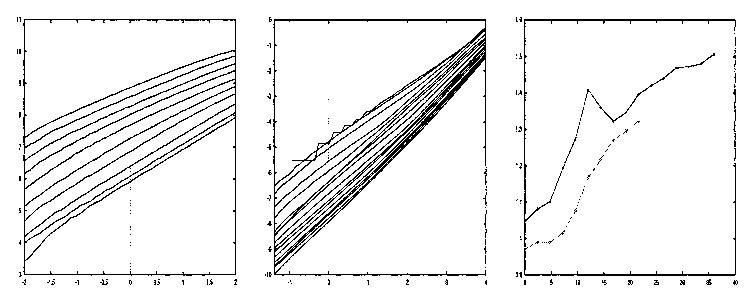
\includegraphics{chap04-vend-scan-09.eps}
\end{figure}

\noindent (The group of \emph{matrices} requires for its generation the additional element $-I$.)

Consider the cycles. There are 4 vertices: $\infty$, $\rho_{1}=1/2+i\sqrt{3}/2,\,\rho_{2}=-1/2+i\sqrt{3}/2$, and $i$. The point $\infty$ is itself a parabolic cycle, $\Gamma_{\infty}$ being generated by $U$. The point $i$ constitutes a cycle of angle $\pi$; hence $T^{2}=I$. The points $\rho_{1},\,\rho_{2}$ are conjugated by $TU$. Since the angle at each vertex is $\pi/3$, we have $(TU)^{3}=I$. (Cf. Th. \ref{ch04:sec4C}.)

Note that $\Gamma(1)$ can also be generated by $T$ and
\begin{equation*}
W=TU=\left(\begin{matrix}
0 & -1\\1 & 1
\end{matrix}\right).
\end{equation*}
The relations become
\begin{equation*}
T^{2}=W^{3}=I.
\end{equation*}
We shall see later that these two relations form a basis for the set of relations in the modular group (\ref{ch07:chap07}. Th. \ref{ch07:sec2F}).


\skiptoctrue
\section*{Exercise}

1. Two different groups can have the same fundamental region. [Consider the groups
\begin{align*}
&G=\bigg\{\left(\begin{matrix}
1 & 0\\1 & 1
\end{matrix}\right),\,\left(\begin{matrix}
3 & 8\\1 & 3
\end{matrix}\right),\,\left(\begin{matrix}
1 & 8\\0 & 1
\end{matrix}\right)\bigg\},\\
&H=\bigg\{\left(\begin{array}{rr}
-3 & 2\\1 & -1
\end{array}\right),\,\left(\begin{array}{rr}
-1 & 2\\1 & -3
\end{array}\right),\,\left(\begin{array}{rr}
1 & 8\\0 & 1
\end{array}\right)\bigg\}.
\end{align*}
Both $G$ and $H$ can be considered as free products of the groups generated by the matrices shown. But $G\neq H$, for $G$ is a subgroup of
\begin{equation*}
\Gamma^{0}(8)=\bigg\{\left(\begin{matrix}
a & b\\c & d
\end{matrix}\right),\,a,\,b,\,c,\,d\ \mathrm{integers},\,b\equiv0 (\mathrm{mod}\ 8)\bigg\}
\end{equation*}
and $H$ is not. Actually $G=\Gamma^{0}(8).]$

\section{Principal-Circle Groups: Isometric Circles}\label{ch04:sec6}\index{isometric circle}

The major class of discontinuous function groups are the principal-circle groups, those groups each element of which preserves the interior of a fixed circle or one side of a fixed straight line. In this Section we shall treat these groups by means of isometric circles. In the next Section we shall follow Poincar\'{e}'s\index{Poincar\'{e}} original method, namely, the exploitation of his circle model of hyperbolic geometry.

\subsection{}\label{ch04:sec6A} Let $\Gamma$ be a principal-circle group. The fixed circle (or line) preserved by each element of $\Gamma$ is called the \emph{principal circle}. By means of a transformation we can always map the principal circle onto the unit circle $\mathscr{Q};|z|=1$. \emph{We shall assume this has been done: the principal circle of} $\Gamma$ \emph{is} $\mathscr{Q}$. The elements of $\Gamma$ are then of the form (\ref{ch02:chap02}.~\ref{ch02:sec9E})
\begin{equation*}
V=\left(\begin{matrix}
a & \bar{c}\\c & \bar{a}
\end{matrix}\right),\qquad a\,\bar{a}-c\,\overline{c}=1.
\end{equation*}

$\Gamma$ contains no loxodromic elements. An elliptic transformation has two fixed points inverse to $\mathscr{Q}$ and not on $\mathscr{Q}$. A parabolic element has a single fixed point\index{$\mathscr{L}$= set of limit points} on $\mathscr{Q}$. A hyperbolic element has two fixed points on $\mathscr{Q}$.

$\mathscr{L}$, the set of limit points of $\Gamma$, lies on $\mathscr{Q}$. For $\mathscr{Q}$ is closed and invariant under each element of $\Gamma$, so we can apply \ref{ch03:chap03}. Th. \ref{ch03:sec4J}. Denote the interior and exterior of $\mathscr{Q}$ by $\mathscr{U}$ and $\mathscr{V}.$ It follows that $\mathscr{U}$ and $\mathscr{V}$ consist entirely of ordinary points. In particular, the fixed points of an elliptic element of $\Gamma$ are always ordinary points.

There are two types of principal-circle groups. $\Gamma$ of the \emph{first kind} or \emph{horocyclic}\index{principal-circle group!of first kind (horocyclic)} if $\mathscr{L}=\mathscr{Q}$, otherwise $\Gamma$ is of the \emph{second kind}\index{principal-circle group!of second kind}. In the latter case $\mathscr{L}$ is either a perfect nowhere dense set or it consists of one or two points (\ref{ch03:chap03}. Th. \ref{ch03:sec5F}). In all cases $\Gamma$ is a function group. When $\Gamma$ is horocyclic, there are two domains of existence: $\mathscr{D}_{1}=\mathscr{U},\,\mathscr{D}_{2}=\mathscr{V}$. otherwise there is a single domain, namely, $\mathscr{D}=\mathscr{Z}-\mathscr{L}$.


\subsection{}\label{ch04:sec6B} In this Section\index{fundamental region!of principal-circle group}\index{principal-circle group!generation of} we assume $\infty$ is not fixed by any element of $\Gamma$. Therefore each $V\in\Gamma-I$ possesses an isometric circle. Furthermore, the isometric circles are orthogonal to $\mathscr{Q}$ (\ref{ch02:chap02}.~\ref{ch02:sec10C}). Since $\infty$ is an ordinary point, we have $|c|>\tilde{c}>0$ when $c \neq 0$ (cf. \ref{ch03:chap03}. Ex. 1-1).

Let $R$ be the standard fundamental region for $\Gamma$. Then, defining $R^{+}$ by
\begin{equation}
\label{ch04:eqn9}
R^{+}=R\cap \mathscr{U},
\end{equation}
we see that $R^{+}$ is a fundamental region relative to $\mathscr{U}$. Similarly, $R^{-}=R\,\cap\,\mathscr{V}$ is a fundamental region relative $\mathscr{V}$. Note that $R^{+}$ contains a neighborhood of the center of $\mathscr{U}$. For otherwise every neighborhood of the center meets infinitely many isometric circles and the center is not an ordinary point.

The inversion $\zeta:z\rightarrow 1/\bar{z}$ maps each isometric disk on itself and maps $\mathscr{U}$ on $\mathscr{V}$. Hence $\zeta$ interchanges $R^{+}$ and $R^{-}$. It will therefore be sufficient to study $R^{+}$.

Let $\mathscr{D}$ be a domain of existence of $\Gamma$. If $\Gamma$ is horocyclic, we choose $\mathscr{D}=\mathscr{U}$. In that case $R_{0}=R\cap \mathscr{D}$ is simply $R^{+}$. When $\Gamma$ is not horocyclic, we have $R_{0}=R^{+}\cup R^{-}\cup \mathscr{F}$, where
\begin{equation*}
\mathscr{F}=R\cap \mathscr{Q}=R\cap\{\mathscr{Q}-\mathscr{L}\}.
\end{equation*}
Since $\mathscr{F}$, when considered as a linear set, is open and nonempty, we have
\begin{equation*}
\tag{${^\ast}$} \mathscr{F}\ =\bigcup_{i}f_{i},
\end{equation*}
where $f_{i}$ is a maximal open arc (component) lying in $\mathscr{Q}$ and the family $\{f_{i}\}$ is countable and disjoint (\ref{ch02:chap02}.~\ref{ch02:sec2I}). Each $f_{i}$ is called a \emph{free side}\index{free side} of $R^{+}($ and of $R^{-})$. Cf. Figure. \emph{The word ``side'' shall refer, as previously, to an arc of an isometric circle}.

In view of \eqref{ch04:eqn9} we may deduce theorems about $R^{+}$ by referring to our previous results on $R$ and taking intersections with $\mathscr{U}$. Thus any compact subset\index{compact subset covered by finitely many fundamental regions} of $\mathscr{U}$ is covered by a finite set of images of $\bar{R}^{+}$ (Th. \ref{ch04:sec1F}). The boundary of $R^{+}$ consists of countably many pairs of conjugate sides and their points of accumulation, and of countably many free sides---cf. Th. \ref{ch04:sec3B} and $(^{\ast})$. When $R^{+}$ has a finite number of sides, there are no points of accumulation of the sides that do not lie on the sides. When $R^{+}$ is bounded by an infinite number of sides there is always at least one point whose neighborhood intersects infinitely many sides or free sides; such a point may or may not lie on a side.

The transformations $\{T_{i}\}$ that map a side of $R^{+}$ on its conjugate side form a set of generators for $\Gamma$. This follows from Theorem 5D. For suppose $\Gamma$ is of the first kind; then $R_{0}=R^{+}$ and the result is just that theorem. If $\Gamma$ is of the second kind, then to each $s_{i}$ of $R^{+}$ there corresponds a side $\zeta s_{i}$ of $R^{-}$, and conversely. Let $T_{i}s_{i}=s_{i}^{\prime}$, then $T_{i}\zeta s_{i}=\zeta s_{i}^{\prime}$. Thus $\{T_{i}\}$ is the full set of elements of $\Gamma$ which conjugate sides of $R_{0}$, and so $\{T_{i}\}$ generates $\Gamma$.

\begin{figure}[!h]
\includegraphics{chap04-vend-scan-10.eps}
\end{figure}


\begin{theorem*}
$R^{+}$ is a simply connected region \emph{(3J)}.
\end{theorem*}

We know $R^{+}$ is open. We assert that a line segment $l$ joining the origin to any point $z$ of $R^{+}$ lies entirely in $R^{+}$. Otherwise there is a point $z_{0}$ on $l$ nearest the origin which is a boundary point of $R^{+}.$ Since $z_{0}$ is an ordinary point, it lies on an isometric circle $\Im$. Since $\Im$ is orthogonal to $\mathscr{Q}$, the line segment $z_{0}z$ lies inside $\Im$ except for $z_{0}$. Hence $z$ is inside $\Im$ and so is not a point of $R^{+}$. This contradiction proves our statement.

It follows that $R^{+}$ is arcwise connected, for any two of its points may be connected by means of line segments drawn from the points in question to the origin. Hence $R^{+}$ is connected (\ref{ch02:chap02}.~\ref{ch02:sec3I}) and so is a region.

The argument in the first paragraph shows also that a radius meets $\mathrm{Bd}\ R^{+}$, if at all, in exactly one point. Hence if we include free sides, $R^{+}$ is a star with respect to the origin and we can describe its boundary by a function $e^{i\theta}f(\theta),\,0<f(\theta)\leqq 1,\, 0\leqq\theta<2\pi$. Now $f$ is continuous. In fact, suppose $f(\theta_{n})\rightarrow\lambda$ as $\theta_{n}\rightarrow\theta^{\ast}$. Then $e^{i\theta^{\ast}}\lambda$ is a boundary point of $R^{+}$ because each $e^{i\theta_{n}}f(\theta_{n})$ is. Hence $e^{i\theta^{\ast}}\lambda=e^{i\theta}f(\theta^{\ast})$, for there is only one boundary point at $\theta=\theta^{\ast}$, and this shows $f$ to be continuous. Every point of $R^{+}$ is of the form $\rho e^{i\theta}f(\theta)$ with $0\leqq \rho\ <1$, and the mapping which sends this point into the point $\rho e^{i\theta}$ is easily seen to be a homeomorphism of $R^{+}$ onto the unit disk.\:\:\:q.e.d.

\subsection{}\label{ch04:sec6C} An ordinary cycle\index{fundamental region!boundary of} of $R_{0}$ lies entirely in $R^{+}$, entirely in $R^{-}$, or entirely on $\mathscr{Q}$. The ordinary cycles of $R^{+}$ are either accidental\index{cycle!accidental} $(l=1)$ or elliptic\index{cycle!elliptic}\index{fixed point!elliptic} of order $l\geqq2$, the sum of the angles\index{cycle!angle sum of} at the vertices of a cycle being $2\pi/l$. The converse also holds (Th. \ref{ch04:sec4C}). Since elliptic fixed points do not lie on $\mathscr{Q}$. Theorem 4E can be strengthened:


\begin{theorem*}
Every elliptic fixed point is a point of an elliptic cycle.
\end{theorem*}

An elliptic cycle cannot lie on $\mathscr{Q}$, but an accidental cycle may (Ex. 6-4). The sum of the angles in $R$ at the vertices of the cycle is $2\pi$. Since each angle is bisected by $\mathscr{Q}$, we have: \emph{the sum of the angles in $R^{+}$ at the vertices of an accidental cycle lying on $\mathscr{Q}$ is} $\pi$.

\subsection{}\label{ch04:sec6D} The parabolic\index{cycle!parabolic}\index{vertex!parabolic} cycles lie on $\mathscr{Q}$. Theorem 4G can be improved. If $p$ is a parabolic vertex, $\Gamma_{p}$ (and not only $\Gamma_{p}^{\ast}$) is a cyclic group generated by a parabolic transformation. This is again due to the fact that there are no elliptic transformations having $p$ as a fixed point. Cf. 41.


\subsection{}\label{ch04:sec6E} Whether $\Gamma$ is\index{principal-circle group!of first kind (horocyclic)} of the first or second kind can be detected from the fundamental region $R$.


\begin{theorem*}
If $\Gamma$ is of the first kind, $R$ does not meet $\mathscr{Q}$\emph{;} if $\Gamma$ is of the second kind\index{principal-circle group!of second kind}, $R$ does meet $\mathscr{Q}$.
\end{theorem*}

Suppose $z_{0}$ is a point of $\mathscr{Q}$ as well as a point of $R$. Then $z_{0}$ is an ordinary point. $\mathscr{Q}$ contains ordinary points, so $\Gamma$ is of the second kind.

Now suppose $\Gamma$ is of the second kind. The domain of existence $\mathscr{D}$ of $\Gamma$ contains arcs on $\mathscr{Q}$. Let $z_{0}\in \mathscr{Q}$ be a point of $\mathscr{D}$, and let $O$ be a neighborhood of $z_{0}$ contained in $\mathscr{D}$. We may obviously select $O$ so that $\bar{O}$ is a compact\index{fundamental region!compact} subset of $\mathscr{D}$. Then $\bar{O}$ is covered by a finite number of images of $R$ (Th. \ref{ch04:sec1F}). Let $z_{0}$ lie in $VR$ for some $V\in \Gamma$; then $V^{-1}z_{0}\in R$ and $V^{-1}z_{0}$ lies on $\mathscr{Q}$.\:\:\:q.e.d.

\subsection{}\label{ch04:sec6F} The fundamental region $\bar{R}$ is a \emph{polygon}\index{fundamental region!is a polygon} or \emph{generalized polygon} in the sense of the following definition.


\begin{definition*} An open set $A$ is a Jordan region provided there is a homeomorphism $f$ such that $f(A)=D$, an open disk, while $f(\overline{A})=\overline{D}$. A \emph{polygon} is a Jordan region whose boundary $\gamma$ satisfies the following conditions.

1) $\gamma=\bigcup\limits^{n}_{i=1}l_{i}$, where $l_{i}$ is a Jordan arc (homeomorph of a closed interval)

2) for $i\neq j,\,l_{i}$ meets $l_{j}$, if at all, in a common endpoint.
\end{definition*}
A \emph{generalized polygon} is defined by replacing $1)$ by
\begin{equation}
\tag{$1^{\prime}$}
\gamma= \mathrm{Cl} \displaystyle \bigcup_{i=1}^{\infty}l_{i}.
\end{equation}
The assumption that the polygon is a Jordan region implies that its boundary $\gamma$ is a simple closed curve. In the case of the generalized polygon, $\gamma$ consists of denumerably many arcs $l_{i}$ and of the points of accumulation of these arcs. The points of accumulation may or may not lie on the $\{l_{i}\}$.

\begin{theorem*}
If $R^{+}$ is bounded by a finite number of sides and free sides, it is a polygon.
\end{theorem*}

The argument of~\ref{ch04:sec6B} showing that $R^{+}$ is simply connected also shows it is a Jordan region. The ordinary points of $\mathrm{Bd}\ R^{+}$ lie on sides or free sides. The limit points on the boundary lie on isometric circles, that is, on sides of $R^{+}$, points of category \textbf{b} 3 being absent because $R^{+}$ has finitely many sides (\ref{ch04:sec3A}). This makes it clear that condition 1) is fulfilled.

Suppose two sides meet. If they meet at an ordinary point (which may be in $\mathscr{U}$ or on $\mathscr{Q})$, the intersection is an ordinary vertex, that is, an endpoint of both sides. When two sides meet at a limit point, they meet on $\mathscr{Q}$ and so at a common endpoint. A side can meet a free side at a point of $\mathscr{Q}$, an endpoint for both. Two free sides can never intersect. This exhausts the possibilities and shows that condition 2) is satisfied,\:\:\:q.e.d.

\subsection{}\label{ch04:sec6G} \begin{theorem*} If $R^{+}$ has a finite number of sides, the only limit points on its boundary\index{fundamental region!boundary of} are parabolic vertices.
\end{theorem*}

We refer for the proof to the classification of limit points lying on the boundary of $R^{+}$ (cf.~\ref{ch04:sec3A}). Points of category \textbf{b} 3 are ruled out because of the finite number of sides. Then a boundary point $\beta$ must lie on one or two isometric circles; if there were, more than two circles issuing from $\beta,\,R^{+}$ would not be a star (Th. \ref{ch04:sec6B}). If $\beta$ lies on a single circle, there must be a free side with endpoint $\beta$, and $\beta$ is not a limit point. Hence two isometric circles issue from $\beta$ and, from the argument of~\ref{ch04:sec4G} and the fact that there are only a finite number of sides, we see that we must return to $\beta$ in a finite number of steps. Hence $\beta$ is a parabolic vertex,\:\:\:q.e.d.

Thus, whereas in the case of the general discontinuous group we shall later have to make an explicit assumption of this result (cf.~\ref{ch05:chap05}.~\ref{ch05:sec4}), for principal-circle groups it follows from the finiteness of the number of sides.

\subsection{}\label{ch04:sec6H} \begin{theorem*} If $R$ is bounded by an infinite number of sides, it is a generalized polygon\index{fundamental region!is a polygon}.
\end{theorem*}


The proof is much the same as the one we have just given. $R^{+}$ is a Jordan region, as before. The boundary of $R^{+}$ consists of sides, free sides, and of points (necessarily on $\mathscr{Q}$) lying near infinitely many sides or free sides. Condition 1$^{\prime}$) is therefore satisfied.

The proof that condition $2)$ is met is the same as before with one change. If a side terminates in a point $q$ of $\mathscr{Q}$ and there is no other side beginning at $q$, there may be infinitely many sides of $R^{+}$ in the neighborhood of $q$. Then $q$ does not affect the intersections of sides.

\skiptoctrue
\section*{Exercises}

1. Let $s,\,s^{\prime}$ be conjugate sides\index{conjugate side} of $R_{0}$ and let $\alpha\in s$ and $\alpha^{\prime}\in s^{\prime}$ be equivalent points. Then $\alpha,\,\alpha^{\prime}$ are at the same distance from the center of the principal circle.

2. The points of a cycle lie on a circle\index{cycle!ordinary} concentric or identical with the principal circle.

3. The euclidean area of $R_{0}$ is larger than that of $V(R_{0})$ for each $V\in\Gamma-I$.

4. Give an example of a principal-circle group for which $R^{+}$ admits an ordinary\index{cycle!ordinary} cycle lying on $\mathscr{Q}$.

[Consider free products of hyperbolic cyclic groups. Make the circles tangent.]

5. The fixed point of a hyperbolic element of $\Gamma$ is never a point of $\bar{R}$ or any of its images.

\section{Principal-Circle Groups: Hyperblic Geometry}\label{ch04:sec7}\index{hyperbolic geometry}\index{principal-circle group}

We shall now construct fundamental regions for principal-circle groups by means of hyperbolic geometry. (Cf.~\ref{ch02:chap02}.~\ref{ch02:sec12}) The hyperbolic concepts will be denoted by prefixing $H:H$-line, $H$-distance, etc. We use the Poincar\'{e}\index{Poincar\'{e}} model, in which the hyperbolic plane is represented by the unit disk $\mathscr{U}:|z|<1$. $H$-points are the usual points, $H$-lines are arcs of circles orthogonal to $\mathscr{Q}$, the boundary of $\mathscr{U}$, and $H$-angle measure is the same as euclidean angle measure. The principal circle of the group is $\mathscr{Q}$.

The reader should note that in texts on Riemann surfaces the discussion is confined to groups of linear transformations with no fixed points in $\mathscr{U}$, which are essentially sufficient for the purpose in hand (cf. \ref{ch06:chap06}. Th. \ref{ch06:sec3K}). Here we allow general discontinuous groups of conformal self-mappings of $\mathscr{U}$. We also allow $\infty$ (and therefore $0$) to be a fixed point.

\subsection{}\label{ch04:sec7A} Let $w_{0}\in \mathscr{U}$ be a nonfixed point. Let $\{V_{i},\,i=0,1,\,2,\cdots;V_{0}=I\}$ be an enumeration of the elements of $\Gamma$. The images $w_{i}=V_{i}w_{0}$ are all distinct. Denote by $\lambda_{i}$ the perpendicular bisector in the hyperbolic sense of the $H$-segment $w_{0}w_{i}$. We mentioned in~\ref{ch02:chap02}.~\ref{ch02:sec12B} that $\lambda_{i}$ is the locus of points $H$-equidistant from $w_{0}w_{i}$. The line $\lambda_{i}$ divides $\mathscr{U}$ into two regions; the one which contains $w_{0}$ we call $L_{i}$. $w\in L_{i}$ if and only if $d(w, w_{0})< d(w,\,w_{i})$, where $d$ denotes $H$-distance.

Define
\begin{equation}
N= \mathrm{Int} \bigcap_{i=1}^{\infty}L_{i}.
\end{equation}
$N$ is called a \emph{normal polygon of $\Gamma$ with center}\index{normal polygon} $w_{0}$. It corresponds to the fundamental region $R^{+}$ of~\ref{ch04:sec6B}, as we shall see later (\ref{ch04:sec7F}).

$N$ is an open subset of $\mathscr{U}$. To show that $N$ is not empty, consider an $H$-disk $K$ about $w_{0}$ of radius $\delta/4$, where $\delta=\min_{i>0}d(w_{0},\,w_{i})$ is positive since $w_{0}$ is an ordinary point and not a fixed point. Now $d(w_{0}, \mathrm{Bd}\ L_{i})=(1/2) d(w_{0},\,w_{i})\geqq\delta/2$; hence $K$ lies in $N$. Moreover, $N$ is $H$-convex. For each $L_{i}$ is $H$-convex, therefore the same is true of $\bigcap_{i} L_{i}$ and so of $N$ (\ref{ch02:chap02}.~\ref{ch02:sec12H}). In consequence $N$ is connected.


\subsection{}\label{ch04:sec7B}
\setcounter{lemma}{0}
\begin{lemma}\label{ch04:lem1} A relatively compact subset of $\mathscr{U}$ meets only a finite number of $\lambda_{i}=\mathrm{Bd}\ L_{i}$.
\end{lemma}

Let $R<\infty$ be an upper bound for the distance from $w_{0}$ to points of $\bar{K}$, where $K$ is the relatively compact subset. Let $w^{\prime}$ be a point of $\lambda_{i}$ lying in $K$. Then
\begin{equation*}
d(w_{0},\,w_{i})\leqq d(w_{0},\,w^{\prime})+d(w^{\prime},\,w_{i})=2d(w_{0},\,w^{\prime})\leqq 2R.
\end{equation*}
That is, $\lambda_{i}$ meets $K$ only if $w_{i}$ lies in the hyperbolic disk of radius $2R$ about $w_{0}$. This disk is compact and can contain only finitely many $w_{i}$.

\begin{lemma}\label{ch04:lem2a} $N=\{w|d(w,\,w_{0})<d(w, w_{j}),j>0\}$.
\end{lemma}

This lemma provides a characterization of $N$ which may be expressed by saying that $N$ consists of those points of $\mathscr{U}$ that are \emph{strictly nearer} $w_{0}$.

It is clear that $N$ is contained in the right member. Suppose conversely that $w$ is a point of the right member; then $w\in\bigcap_{i}L_{i}$. By the preceding lemma there is an open disk containing $w$ which lies in each $L_{i}$. Thus $w\in \mathrm{Int}\bigcap_{i}L_{i}$ and the lemma is proved.

\subsection{}\label{ch04:sec7C} From now on\index{side} we denote $N$ by $N_{0}$ and define
\begin{equation*}
N_{i}=V_{i}N_{0},\qquad V_{i}\in\Gamma.
\end{equation*}
$N_{i}$ consists of those points of $\mathscr{U}$ that are strictly nearer $w_{i}$. The regions $\{N_{i}\}$ are permuted by the transformations of $\Gamma$. Like $N_{0},\,N_{i}$ is nonempty, open, $H$-convex, and connected. It is called a \emph{normal polygon of} $\Gamma$ \emph{with center} $w_{i}$. The family $\{N_{i}\}$ is called a \emph{partition of $\mathscr{U}$ with center} $w_{0}$. The polygons of a partition are mutually $H$-congruent.


\setcounter{lemma}{0}
\begin{lemma}\label{ch04:lem1a}
$N_{i}\cap N_{j}=0$ for $i\neq j$.
\end{lemma}

Suppose $w\in N_{i},\,w\in N_{j}$. Since $w\in N_{i}$ we have $d(w,\,w_{i})<d(w,\,w_{j})$. Since $w\in N_{j}$ we have $d(w,\,w_{j})<d(w,\,w_{i})$, a contradiction.

\begin{lemma}\label{ch04:lem2a1} Two distinct points of $N_{i}$ are inequivalent.
\end{lemma}

Suppose $w_{1},w_{2}\in N_{i}$ and $Vw_{1}=w_{2}$. $V$ maps $N_{i}$ on some $N_{j}$ and so $w_{2}\in N_{j}$, contradicting Lemma~\ref{ch04:lem1a}.

\begin{lemma}\label{ch04:lem3}
$\bigcup_{i}\bar{N}_{i}\supset \mathscr{U}$.
\end{lemma}

Let $w\in \mathscr{U}$. The set $\Gamma w_{0}$ does not accumulate at $w$, this by virtue of the discontinuity of $\Gamma$. Hence there is a $w_{j}$ (perhaps several but only a finite number) that is nearest $w$. If $d(w,\,w_{j})<d(w,\,w_{i})$, $i\neq j$, then $w$ lies in $N_{j}$, by Lemma~\ref{ch04:lem2a1} of~\ref{ch04:sec7B}. If $d(w,\,w_{j})\leqq d(w,\,w_{i})$, $i\neq j$, then by~\ref{ch04:sec7B}, Lemma~\ref{ch04:lem1a}, equality can be attained for only a finite number of $i$. Hence every neighborhood of $w$ contains points of $N_{j}$ and $w$ lies on Bd $N_{j}$. In either case $w\in\bar{N}_{j}$.

\begin{lemma}\label{ch04:lem4}
The sides of $N_{0}$ \emph{(}and so of $N_{i}$\emph{)} are conjugate in pairs. The neighborhood of a point on the boundary of $N_{0}$ contains points of $\sim N_{0}$ equivalent to points of $N_{0}$.
\end{lemma}

A \emph{side} of $N_{0}$ is the part of a perpendicular bisector $\lambda_{i}$ bounding $N_{0}$. Let $T\in\Gamma$ map $N_{0}$ on $N_{i}$ abutting $N_{0}$ along a side $s$. Then $T^{-1}s=s^{\prime}$ is also a side of $N_{0}$, and $s,\,s^{\prime}$ are conjugate sides\index{conjugate side}. It is not hard to show that $s^{\prime}$ is unique. The second statement of the lemma follows in the usual way.

These lemmas suffice to prove the main result:

\setcounter{theorem}{0}
\begin{theorem}\label{ch04:thm1}
$N_{0}$ \emph{(}and therefore $N_{i})$ is a fundamental region for $\Gamma$ relative to $\mathscr{U}$, and $\Gamma\bar{N}_{0}$ covers $\mathscr{U}$.
\end{theorem}

\begin{theorem}\label{ch04:thm2}
Any compact subset\index{compact subset covered by finitely many fundamental regions} of $\mathscr{U}$ is covered by a finite set of $\{\bar{N_{i}}\}$.
\end{theorem}

Let $K$ be the compact subset; we have $d(0, w)<R<\infty$ for all $w\in K$. We have just seen that $K$ is covered by the full set of $\{\bar{N}_{i}\}$. The theorem will be proved if we show that $K$ can meet only finitely many $N_{i}$. Indeed, the $H$-diameter of each $N_{i}$ is the same because $H$-distance is preserved by the mappings of $\Gamma$. And $d(0,\,w_{i})\rightarrow\infty$ with $i\rightarrow\infty$, otherwise there would be infinitely many centers $w_{i}$ lying in the circle $|w|<R$ and these points would accumulate at a point of $\mathscr{U}$. This would contradict the discontinuity of $\Gamma$. If $w_{i}$ lies outside the disk $d(0, w)\leqq R+\mathrm{diameter}\ N_{0}$ for $i>i_{0},\,K$ meets no $N_{i}$ with $i>i_{0}$.\:\:\:q.e.d. Cf. Note 8, p. 400.

\subsection{}\label{ch04:sec7D} The geometry of\index{principal-circle group!generation of} the fundamental region $N_{0}$ is the same as that of $R^{+}$ (cf.~\ref{ch04:sec6B}).


We have defined the \emph{sides} of a normal polygon\index{fundamental region!is a polygon}. The endpoints of a side, in the event they are points of $\mathscr{U}$, are points lying on two or more sides, and are \emph{ordinary vertices}\index{vertex!ordinary}.

If a side $s$ terminates in a point $q$ of $\mathscr{Q}$, there may be another side of $N_{0}$ issuing from $q$, but there cannot be more than one, because of the convexity of $N_{0}$. Suppose there is no side of $N_{0}$ in the neighborhood of $q$ except $s$. Then there is a maximal arc $f$ of $\mathscr{Q}$ beginning at $q$ which forms part of the boundary\index{fundamental region!boundary of} of $N_{0};f$ is a \emph{free side}\index{free side}. Lastly, there may be points $q$ on $\mathscr{Q}$ such that $q$ is a point of accumulation of sides of $N_{0}$ but does not lie on any side.

If $N_{0}$ is bounded by a finite number of sides, the last class of points is empty. Then we deduce easily that $N_{0}$ is a polygon. When $N_{0}$ admits an infinite number of sides it is a generalized polygon. (Cf.~\ref{ch04:sec6F}, H.)

The elements of $\Gamma$ which map the sides of $N_{0}$ on their conjugate sides (\ref{ch04:sec7C}, Lemma~\ref{ch04:lem4}) generate $\Gamma$. This is Theorem 5D for the fundamental region $N_{0}$, and the proof is the same.

\subsection{}\label{ch04:sec7E} The ordinary cycles are either elliptic or accidental\index{cycle!accidental}\index{vertex!accidental, of first kind}, as before. Theorems 4C and 6C hold.

There may be accidental vertices on $\mathscr{Q}$. These are of two types. We shall call $q\in \mathscr{Q}$ an \emph{accidental vertex of the first kind} if $q$ is accidental (i.e., not a fixed point) and if it is the intersection of two sides of $N_{0}$. (Cf. Ex. 6-4.) The point $q$ will be called an \emph{accidental vertex of the second kind} if it is the intersection of a side and a free side. It will be seen later that accidental vertices of the first kind can be avoided entirely by a suitable choice of $w_{0}$, the center of $N_{0}$.

Consider now the parabolic\index{fixed point!parabolic}\index{vertex!parabolic} cycles of $N_{0}$, which are defined exactly as before (\ref{ch04:sec4G}). A parabolic cycle lies on $\mathscr{Q}$. If $(p_{1},\,\cdots,\,p_{s})$ is such a cycle, each $p_{i}$ is the fixed point of a parabolic element $P_{i}$ of $\Gamma$ and the subgroup $\Gamma_{p_{i}}$ is cyclic. Each $p_{i}$ lies on two sides of $N_{0}$ which are tangent at $p_{i}$. (Cf. \ref{ch04:sec4G} and \ref{ch04:sec6D}.)

Now, however, we can prove the converse:


\begin{theorem*}
The fixed point of a parabolic transformation of $\Gamma$ is a vertex of some normal polygon.
\end{theorem*}

As we noticed earlier (\ref{ch04:sec4H}), this theorem is untrue for general discontinuous groups.

Let $p$ be the fixed point of a parabolic transformation $P$ which generates $\Gamma_{p}$. We shall operate in the upper half-plane $\mathscr{H}$. Determine a linear transformation $A$ which maps $\mathscr{U}$ on $\mathscr{H}$, carries $p$ to $\infty$, and carries the center of $N_{0}$ to $i$. The transformed group $\Gamma^{\prime}=A \Gamma A^{-1}$, which is discontinuous in $\mathscr{K}$---cf. \ref{ch03:chap03}.~\ref{ch03:sec1D}, Lemma 2---may be written as a group of matrices $V^{\prime}_{n} = (a_{n}^{\prime}b_{n}^{\prime}|c_{n}^{\prime}d_{n}^{\prime})$ with real entries (\ref{ch02:chap02}.~\ref{ch02:sec9E}). The element $P^{\prime}=APA^{-1}$ generates $\Gamma_{\infty}^{\prime}$ and is a translation $(1\ \lambda^{\prime}\,|\,0\,1)$. The only elements of $\Gamma^{\prime}$ with $c^{\prime}=0$ are the powers of $P^{\prime}.$ For if $V^{\prime}$ fixes $V=A^{-1}V^{\prime}A$ fixes $p$ and so is a power of $P$.

The hyperbolic element of length in $\mathscr{H}$ is $ds=|dw'|/y^{\prime},\,w^{\prime}=x^{\prime}+iy^{\prime}$ (\ref{ch02:chap02}.~\ref{ch02:sec12G}).

\begin{lemma*}
Let $N_{0}^{\prime}$ be the normal polygon\footnote{By the normal polygon of a group defined on $\mathscr{H}$ we mean the polygon formed in a manner strictly analogous to our previous construction. Of course we must use the hyperbolic metric appropriate to $\mathscr{H}$.} for $\Gamma^{\prime}$ relative to $\mathscr{H}$ with center $w_{0}^{\prime}$. Then $N_{0}=A^{-1}N_{0}^{\prime}$ is the normal polygon of $\Gamma$ relative to $\mathscr{U}$ with center $w_{0}=A^{-1}w_{0}^{\prime}$.
\end{lemma*}

Denote by $d,\,d^{\prime}$ the $H$-distances on $\mathscr{U},\,\mathscr{H}$, respectively. Recall that $d(w_{1},\, w_{2})=d^{\prime}(Aw_{1}, Aw_{2})$ for $w_{1},\,w_{2}\in \mathscr{U}$ (cf.~\ref{ch02:chap02}.~\ref{ch02:sec12G}). Let $\lambda_{i},\,\lambda_{i}^{\prime}$ be the bisectors of the segments $w_{0}w_{i},\, w_{0}^{\prime}w_{i}^{\prime}$, respectively, where $w_{i}=V_{i}w_{0},\,w_{i}^{\prime}= AV_{i}A^{-1}w_{0}^{\prime},\, V_{i}\in\Gamma$. Note that $A^{-1}w_{i}^{\prime}=w_{i}$.

Suppse $w\in\lambda_{i}^{\prime}$. Then $d^{\prime}(w^{\prime}, w_{0}^{\prime})=d^{\prime}(w^{\prime}, w_{i}^{\prime})$, which implies $d(A^{-1}w^{\prime}, w_{0})= d(A^{-1}w^{\prime}, w_{i})$, i.e., $A^{-1}w^{\prime}\in\lambda_{i}$. The converse is also true. It follows that $\lambda_{i}=A^{-1}\lambda_{i}^{\prime}$. In other words, the bisectors of the segments $w_{0}w_{i}$ are the $A^{-1}$-images of the bisectors of the segments $w_{0}^{\prime}w_{i}^{\prime}$.\:\:\:q.e.d.

Consider the images of $i$ under $\Gamma^{\prime}$:
\begin{equation*}
V_{n}^{\prime}(i)=\cdots+i(c^{\prime{2}}_{n}+d^{\prime{2}}_{n})^{-1}.
\end{equation*}
If $c_{n}^{\prime}=0,\,d_{n}^{\prime}=\pm 1$, as we have seen. Otherwise $|c_{n}^{\prime}|\geqq\tilde{c}>0$, as we shall prove in \ref{ch08:chap08}. Th. \ref{ch08:sec2D}. Hence $\mathrm{Im}\ V_{n}^{\prime}(i)$ is bounded above. Let $V_{k}^{\prime}(i)=w^{\prime}_{k}$ be a point of $\Gamma^{\prime}i$ of maximum imaginary part.

We shall use $w^{\prime}_{k}$ as the center of a normal polygon $N_{k}^{\prime}$. Let $L$ be the horizontal line passing through $w_{k}^{\prime}$. The only images of $w_{k}^{\prime}$ lying on $L$ are the points $w_{k,m}^{\prime}=w_{k}^{\prime}+m\lambda^{\prime},\,m=\mathrm{integer}$. The hyperbolic line $w_{k}^{\prime}w_{k,m}^{\prime}$ has as hyperbolic midpoint the euclidean midpoint of the arc of the circle passing through $w^{\prime}_{k},\,w_{k,m}^{\prime}$ and orthogonal to the real axis. This follows because $w_{k}^{\prime},\,w_{k,m}^{\prime}$ are at the same height above the real axis, and is easily checked by symmetry from the formula for hyperbolic arc length given above. Hence the $H$-bisector of the $H$-segment $w_{k}^{\prime}w_{k,m}^{\prime}$ is identical with the euclidean bisector of the euclidean segment $w_{k}^{\prime}w_{k,m}^{\prime}$. The bisectors nearest $w_{k}^{\prime}$ bound a vertical strip $\mathscr{S}$, part of which, as we now show, lies in $N_{k}^{\prime}$.

Indeed, let $\Omega=\Gamma^{\prime}i-\{w_{k,m}^{\prime},\,m=0,\,\pm 1,\cdots\}.$ $\Omega$ lies below $L$. Because of the discontinuity of $\Gamma$ there is a point of $\Omega$ (or perhaps a finite number of points) which lies nearest $w_{k}^{\prime}$. The hyperbolic circle $C$ with center at $w'=x^{\prime}+iy^{\prime}\in \mathscr{S}$ and passing through $w_{k}^{\prime}=x_{k}^{\prime}+iy_{k}^{\prime}$ has the equation (\ref{ch02:chap02}. Ex. 12-1)
\begin{equation*}
(\xi-x^{\prime})^{2}+(\eta-y^{\prime{2}}\cosh\rho)^{2}=y^{\prime2{}}\sinh^{2}\rho,
\end{equation*}
where $\rho =d(w^{\prime}, w_{k}^{\prime})$. The slope of the tangent to $C$ at $w_{k}^{\prime}$ is
\begin{equation*}
(x^{\prime}-x_{k}^{\prime})/(y_{k}^{\prime}-y^{\prime}\cosh\rho)
\end{equation*}
and this tends to 0 as $y^{\prime}$ (and therefore $\rho$) tend to $\infty$. We see that $C$ tends to the line $L$ as $y^{\prime}\rightarrow\infty$. Hence for all $w^{\prime}\in \mathscr{S}$ lying above a certain horizontal line $L^{\prime}$, the circle in question does not contain any point of $\Omega$. It follows that $w^{\prime}\in N_{k}^{\prime}$, for $w^{\prime}$ is nearer $w_{k}^{\prime}$ than it is to any point of $\Omega$, and so $w^{\prime}$ is as near to $w_{k}^{\prime}$ as it is to any point of $\Gamma_{i}^{\prime}$. That is, all that part of $\mathscr{S}$ lying above $L^{\prime}$ belongs to $N_{k}^{\prime}$. This says that $N^{\prime}_{k}$ contains $\infty$; then, by the Lemma, $N_{k}$ contains $p$.\:\:\:q.e.d.

\subsection{}\label{ch04:sec7F} The reader will have noticed that the fundamental regions $N_{0}$ and $R^{+}$ (cf.~\ref{ch04:sec6B}) have many properties in common. The exact connection between the two is as follows:


\begin{theorem*}
$R^{+}$ is that normal polygon\index{fundamental region!standard, and normal polygon} whose center is the origin.
\end{theorem*}

We have to assume, of course, that $\infty$ (and therefore $0)$ is not a fixed point. The theorem will be proved if we show that the $H$-bisector of the $H$-line connecting $0$ and $V(0)$ is part of the isometric circle $\Im(V^{-1})$.

The $H$-line joining $0$ and $V(0)$ is identical with the euclidean segment $l$ joining the same points. Set $V=(a\,\bar{c}\,|\,c\,\bar{a}),\,a\bar{a}-c\bar{c}=1$. By a preliminary rotation we may assume that $a/c$, the center of $\Im(V^{-1})$, is real and positive; then $V(0)=\bar{c}/\bar{a}$ is real and positive.

Let $\alpha$ be the $H$-midpoint of $l.$ A simple calculation using~\ref{ch02:chap02}.~\ref{ch02:sec12}. (20) shows that
\begin{equation*}
\beta\alpha^{2}-2\alpha+\beta=0,\qquad\beta=\bar{c}/\bar{a}.
\end{equation*}
The $H$-bisector of $l$ is an arc of a circle $C$ orthogonal to $\mathscr{Q}$, and $C$ cuts the real axis at $\alpha$ and $1/\bar{\alpha}=1/\alpha$. The center of $C$ is therefore
\begin{equation*}
\frac{1}{2}\left(\alpha+\frac{1}{\alpha}\right)=\frac{1}{\beta}=\frac{\bar{a}}{\bar{c}}=\frac{a}{c}.
\end{equation*}
Since this is also the center of $\Im(V^{-1})$, the two circles must be identical, for both are orthogonal to $\mathscr{Q}$.

\begin{corollary*}
The fixed point of a parabolic\index{fixed point!parabolic} transformation of $\Gamma$ is a vertex of $R^{+}$ or of one of its $\Gamma$-images.
\end{corollary*}

It would be interesting to have a proof of this based on the theory of isometric circles.

\subsection{}\label{ch04:sec7G} The center $w_{0}$ of the normal polygon $N_{0}$ may be chosen as any point of $\mathscr{U}$ which is not fixed by an element of $\Gamma$. We can use this freedom of choice to obtain a polygon $N_{0}$ with certain desirable features.

\begin{theorem*}
If $w_{0}$ avoids a certain subset of $\mathscr{U}$ of plane measure $0$, the polygon $N_{0}$ with center $w_{0}$ has the following properties:\index{normal polygon!with special properties}

\emph{1)} Each elliptic and parabolic cycle consists of a single vertex\index{cycle!of single vertex}.

\emph{2)} There are no accidental\index{vertex!accidental, of first kind}\index{vertex!accidental, of second kind} vertices of the first kind lying on $\mathscr{Q}$---\emph{ch.~\ref{ch04:sec7E}}.
\end{theorem*}

We consider elliptic cycles first. Let $\alpha_{1}$, an elliptic fixed point, be the initial point of a side $s$ and let $\alpha_{2}$ be the terminal point of the conjugate side $s^{\prime}$. Then $\alpha_{1}, \alpha_{2}$ are elements of an elliptic cycle and there is a $V\in \Gamma$ such that $V\alpha_{1} =\alpha_{2}$. $V$ maps $N_{0}$ on an adjacent polygon $N_{k}$ with center $w_{k}$. Hence $d(\alpha_{1},\,w_{0})=d(\alpha_{2},\, w_{k})=d(\alpha_{2},\,w_{0})$, since $s^{\prime}$ is the perpendicular bisector of $w_{0}w_{k}$. This shows that $w_{0}$ is equidistant (in the hyperbolic sense) from $\alpha_{1}$ and $\alpha_{2}$ and so lies on the perpendicular bisector of $\alpha_{1}\alpha_{2}$.

Now draw the bisectors of all segments $\alpha\beta$ where $\alpha$ and $\beta$ range independently over all elliptic fixed points. This gives a countable set of lines. Each line is of plane measure zero; so, therefore, is the countable set of lines. Any point $w_{0}$ which avoids this set of lines (and which is not a fixed point) serves as the center of a polygon $N_{0}$ which has no elliptic cycle having more than one vertex.

Before considering parabolic cycles we note a geometrical

\begin{lemma*}
Let $w_{0}, w_{1},\,w_{2}\in \mathscr{U}.$ If the $H$-bisector of $w_{0}w_{1}$ cuts $\mathscr{Q}$ at $q$, then $w_{0},\,w_{1}$, and $q$ lie on $a$ euclidean circle tangent to $\mathscr{U}$ at $q$. If the bisectors of $w_{0}w_{1}$ and $w_{0}w_{2}$ meet at $q$, the same statement is true of the points $w_{0},\,w_{1},\,w_{2}$, and $q$.
\end{lemma*}

Map $\mathscr{U}$ onto the upper half-plane, sending $q$ to $\infty$ and $w_{i}$ to $w_{i}^{\prime},\,i=0,1,2$. The $H$-bisector of $w_{0}w_{i}$ goes into a vertical line $\lambda_{i}$. The $H$-line $w_{0}^{\prime}w_{i}^{\prime}$, which is a euclidean circle with center on the real axis, must cut $\lambda_{i}$ orthogonally. The point $w_{i}^{\ast}$ on $w_{0}^{\prime}w_{i}^{\prime}$ at the same height as $w_{i}^{\prime}$ is therefore a point such that $w_{i}^{\ast}w_{0}$ is bisected by $\lambda_{i}$, as follows from considerations of symmetry. Since there is only one such point, we have $w_{i}^{\ast}=w_{i}^{\prime}$. The points $w_{0}^{\prime},\,w_{1}^{\prime},\,w_{2}^{\prime}$ lie on a horizontal line, which means that $w_{0},\,w_{1},\,w_{2}$ lie on a circle of the required type,\:\:\:q.e.d.

Now suppose $p_{1}$ is a member of a parabolic cycle containing at least one other vertex. Let $s_{1}$ be the side of $N_{0}$ beginning at $p_{1}$; then $s_{1}^{\prime}$ ends at $p_{2}$, say, and $p_{2}$ is in the cycle. Let $V\in\Gamma$ map $s_{1}$ on $s_{1}^{\prime}$; $V^{-1}N_{0}=N_{1}$ is a polygon bordering $N_{0}$ along $s_{1}$ and $N_{1}$ has a parabolic vertex at $p_{1}$. Let $V_{1}(w_{0})=w_{1};w_{1}$ is the center of $N_{1}$ and the bisector of $w_{0}w_{1}$ goes through $p_{1}$. According to the lemma just proved, $w_{0}$ and $w_{1}$ lie on a circle tangent to $\mathscr{Q}$ at $p_{1}$. Note that $V_{1}$ does not fix $p_{1}$.

We now transform to the upper half-plane by a mapping $A$ which sends $p_{1}$ to $\infty$. Then we can say: the group $\Gamma^{\prime}=A\Gamma A^{-1}$ admits a parabolic cycle of more than one vertex containing $\infty$ only if there is a $V^{\prime}\in\Gamma^{\prime}$, not fixing $\infty$, such that $w_{0}^{\prime}$ and $w_{1}^{\prime}=V^{\prime}w_{0}^{\prime}$ lie on a horizontal line. (\emph{If} $V^{\prime}$ fixes $\infty$, we have a cycle of one vertex.) Write the transformations of $\Gamma^{\prime}$ as $V^{\prime}=(a\,b\,|\,c\,d)$. Setting $w_{0}^{\prime}=x+iy,\,w_{1}^{\prime}=x^{\prime}+iy^{\prime}$, the condition becomes $y^{\prime}=y$, where $y^{\prime}=y|cz+d|^{-2}$. That is, $|cz+d|=1$. We also have $c\neq 0$, since $V^{\prime}$ does not fix $\infty$. Now $|cz+d|=1,\,c\neq 0$ is the equation of a circle determined by $V^{\prime}$. Any $w_{0}\in \mathscr{U}$ such that $w_{0}^{\prime}$ avoids this countable set of circles in. $\mathscr{H}$ (i.e., $w_{0}$ avoids a certain countable
set of circles in $\mathscr{U})$, and which is not a fixed point of $\Gamma$, may be used as the center of a polygon $N_{0}$ whose parabolic cycle at $p_{1}$ consists of $p_{1}$ alone. Again we see that $w_{0}$ must be selected outside a certain set of plane measure zero.

Finally, we treat accidental vertices of the first kind lying on $\mathscr{Q}$. The situation here is the following: there are 3 adjacent polygons with centers $w_{0},\,w_{1},\,w_{2};$ the $H$-bisectors of $w_{0}w_{1},\,w_{0}w_{2}$ meet at a point $q\in \mathscr{Q}$ and $q$ is not a fixed point. We wish to show that the points $w_{0}$ for which this happens form a set of measure zero.

By the lemma proved above, $w_{0},\,w_{1},\,w_{2}$ lie on a circle tangent to $\mathscr{Q}$. There are $V_{i}\in\Gamma$ such that $V_{i}w_{0}=w_{i},\,i=1,2$. The above condition on $w_{0},\,w_{1},\,w_{2}$ becomes, when we transform to the upper half-plane, that the 3 images $w^{\prime}_{0},\,w^{\prime}_{1},\, w^{\prime}_{2}$ lie on a circle tangent to the real axis or on a horizontal line. Now this condition can be expressed algebraically and leads to an algebraic equation in $x,\,y$, the coordinates of $w_{0}$, with coefficients that depend only on the coefficients of $V_{1}$ and $V_{2}$. If not all the coefficients of this algebraic equation vanish, the locus of those $w_{0}$ satisfying the given geometric condition is an algebraic curve (perhaps several disjoint curves). Thus if we allow $V_{1}$ and $V_{2}$ to range over $\Gamma$, the $w_{0}$ which could possibly produce an accidental vertex on $\mathscr{Q}$ will lie on a countable set of algebraic curves.

If, on the other hand, all the coefficients of the above algebraic equation do vanish for a certain choice of $V_{1},\,V_{2}$, then every $w_{0}\in \mathscr{U}$ is the center of a polygon which has a vertex on $\mathscr{Q}$, the adjacent polygons being its images by $V_{1}$ and $V_{2}$. What we must show is that this is impossible unless $V_{1}, V_{2}$ are parabolic with common fixed point. In that case, however, the vertex is parabolic, not accidental.

Denote by $V_{1}^{\prime},\,V_{2}^{\prime}$ the transforms of $V_{1},\,V_{2}$ in the upper half-plane. Suppose first $V_{1}^{\prime}$ and $V_{2}^{\prime}$ do not have a common fixed point; let $\alpha$ be a fixed point of $V_{1}^{\prime}$. If $w_{0}^{\prime}$ (and therefore $w_{1}^{\prime}$) approach $\alpha,\,w_{2}^{\prime}$ approaches $\beta=V^{\prime}_{2}\alpha$, and $\beta\neq \alpha$ by our assumption. The center of the circle $C$ passing through $w_{0}^{\prime}, w_{1}^{\prime},
w_{2}^{\prime}$, is the intersection of the euclidean bisectors $\lambda_{1},\,\lambda_{2}$ of $w_{0}^{\prime}w_{1}^{\prime}$ and $w_{0}^{\prime}w_{2}^{\prime}$, respectively. As $w_{0}^{\prime}\rightarrow\alpha,\,\lambda_{2}$ tends to a fixed line, the bisector of $\alpha\beta$. On the other hand, by varying the mode of approach of $w_{0}^{\prime}$ to $\alpha$ we can make $\lambda_{1}$ assume any inclination whatever. For example, if $V_{1}^{\prime}$ is parabolic, let $w_{0}^{\prime}\rightarrow \alpha$ along a fixed circle $K$ of $V_{1}^{\prime};w_{1}^{\prime}\rightarrow\alpha$ along the same line. $\lambda_{1}$ is a line through the center of $K$; its inclination depends on the position of $w^{\prime}_{0}$. In particular we can make the meeting point of $\lambda_{1}$ and $\lambda_{2}$ (i.e., the center of $C$) lie in the lower half-plane. Then $C$ is not tangent to the real axis. Similar constructions are possible for nonparabolic $V_{1}^{\prime}$.

We are therefore forced to assume that $V_{1}^{\prime}$ and $V_{2}^{\prime}$ have a common fixed point. Suppose $V^{\prime}_{1}$ hyperbolic, then $V_{2}^{\prime}$ cannot be parabolic, else $\Gamma^{\prime}$ is not discontinuous (\ref{ch03:chap03}. Cor. \ref{ch03:sec2E}). If $V_{2}^{\prime}$ is hyperbolic, assume the common fixed points are $0$ and $\infty$. Then $w_{0}^{\prime},\,w_{1}^{\prime}, w_{2}^{\prime}$, lie on a line through the origin. $V_{2}^{\prime}$ cannot be elliptic, for in a principal-circle group on, $\mathscr{H}$ the fixed points of elliptic transformations are not real. By the same token, $V_{1}^{\prime}$ cannot be elliptic and $V_{2}^{\prime}$ parabolic. If both $V_{1}^{\prime}$ and $V_{2}^{\prime}$ are elliptic, the 3 points are already on a (fixed) circle, and this circle is not tangent to the real axis if it is small enough. The only remaining possibility is that $V_{1}^{\prime},\,V_{2}^{\prime}$, are parabolic with common fixed point. Our assertion regarding accidental vertices is now proved.

We have seen that we can obtain a normal polygon each of whose elliptic cycles consists of a single vertex by choosing its center outside of a certain set of plane measure zero. We can do the same for the parabolic and accidental cycles. It is evident that the set which $w_{0}$ must avoid is the union of 3 sets of plane measure zero. The theorem is now completely proved.

\subsection{}\label{ch04:sec7H} Let $q_{1}$ be an accidental vertex of the second kind and $s_{1}$ the side issuing from $q_{1}$. Suppose $s_{1}^{\prime}$ ends in $q_{2}$, another accidental vertex of the second kind. Then we cannot continue the process (\ref{ch04:sec4G}) of finding additional vertices of the cycle, since no side issues from $q_{2}$. The vertices $q_{1},\,q_{2}$ form an \emph{open} cycle. Obviously the sum of the angles in $N_{0}$ at the vertices of this cycle is $\pi$.

In general there is another side $s_{2}$ issuing from $q_{2}$. The process yields an open cycle $(q_{1}, q_{2},\,\cdots,\, q_{s})$, where $q_{1},\,q_{s}$ are accidental vertices of the second kind and the remaining vertices are accidental of the first kind. The angle sum of this cycle is still $\pi$.

Theorem 7G shows that by choice of center we can avoid accidental vertices of the first kind. \emph{Hence we can avoid all accidental cycles on} $\mathscr{Q}$ \emph{except those consisting of} $tuo$ \emph{vertices of the second kind}.


\skiptoctrue
\section*{Exercises}

1. If $q$ is an inner point of a free side of $N_{i}$, then $q$ is not equivalent to any other point of $N_{i}$.

2. The subgroup $\Gamma_{a}$, where $a$ lies in $\bar{N}_{i}$, is either the identity or a cyclic group.

3. Show that the fundamental region of a horocyclic group has finite hyperbolic area\index{fundamental region!hyperbolic area} provided it has a finite number of sides. [The calculation is easier in the upper half-plane.]

4. A fundamental region that is relatively compact\index{fundamental region!compact} in $\mathscr{H}$ defines a horocyclic group having no parabolic elements.

%%%%%%%%%%chapter05

\chapter{Automorphic Functions and Forms}\label{ch05:chap05}\index{automorphic form}\index{automorphic function}

Our object in this chapter is to prove the existence and derive some of the properties of automorphic functions on the general discontinuous group. By an automorphic function we mean a meromorphic function which takes the same value at all $\Gamma$-equivalent points.

There are two fundamentally different ways of developing the theory of automorphic functions. Klein\index{Klein, F.} noticed that an automorphic function on $\Gamma$ becomes a single-valued function on the Riemann surface obtained by identifying points which are equivalent under $\Gamma$, and conversely. He could therefore develop the theory of automorphic functions from the known theory of Riemann surfaces. Poincar\'{e}\index{Poincar\'{e}}, on the other hand, wrote down certain infinite series, now called Poincar\'{e} series, which exhibit a simple behavior under transformations of $\Gamma$. A convergent Poincar\'{e} series defines an analytic function $F(z)$ which satisfies the functional equation
\begin{equation}
\label{ch05:eqn1} F(Vz)=(cz+d)^{k}F(z)
\end{equation}
for each $V= (a\,b\,|\,c\,d)\in\Gamma$, where $k$ is a certain integral parameter. The quotient of two Poincar\'{e} series, then, is an automorphic function provided the denominator is not identically zero.

The next chapter will be devoted to the theory of Riemann surfaces and its connection with automorphic functions. In the present chapter we shall explore the Poincar\'{e} series.

The Poincar\'{e} series is an example of an \emph{automorphic form}, a function characterized by the property \eqref{ch05:eqn1}. Automorphic forms are of great interest in themselves and we shall develop their properties systematically. The number $-k$ is called the \emph{dimension} of the form.

There are 3 main problems in the theory of automorphic forms:

1) Prove the existence of nonconstant automorphic forms of each dimension and develop their properties.

2) Provide analytical expressions (e.g., Poincar\'{e} series) which are automorphic forms.

3) Find a family of such analytical invariants which spans or at least is dense in the linear space of automorphic forms of a given dimension.

The third problem is not discussed in this chapter. Cf.~\ref{ch08:chap08} and \ref{ch09:chap09}, where the question is resolved in case $\Gamma$ is a principal-circle group acting on the upper half-plane.

\section{Definition and First Properties}\label{ch05:sec1}

\subsection{}\label{ch05:sec1A}
Let $H$ be a discontinuous group, and let $f$ be a nonconstant function meromorphic in $\mathcal{O}$ (the set of ordinary points of $H$) and invariant on $H$:
\begin{equation}\label{ch05:eqn2}
f(Vz)=f(z)\,\mathrm{for}\,V\in H\qquad\mathrm{and}\,z\in \mathcal{O}.
\end{equation}
We note first that $f$ has an essential singularity\index{automorphic function!singularities of} at every limit point $\lambda$ of $H$. For every neighborhood of $\lambda$ contains infinitely many distinct equivalent points (\ref{ch03:chap03}. Th.~\ref{ch03:sec4A}) and at these points $f$ assumes the same value. It is well known that under these circumstances $f$ is either constant or not meromorphic at $\lambda$.

A corollary of this remark is that an automorphic function invariant on a group that is not discontinuous is either constant or everywhere singular.

Assume $H$ is discontinuous. Let $\mathcal{O}$ be partitioned into the regions of discontinuity $\{\mathscr{D}_{i}\}$; cf. \ref{ch03:chap03}. \ref{ch03:sec5A}. If there are substitutions which map $\mathscr{D}_{i}$ on $\mathscr{D}_{j}$ say, consider the equation \eqref{ch05:eqn2} for a $z$ in $\mathscr{D}_{i}$. Now $Vz$ lies in $\mathscr{D}_{j}$. Since $f$ is meromorphic at $z$, it is also meromorphic at $Vz$. Hence it is possible to continue $f$ analytically from $z$ to $Vz$. But here we have a contradiction, for any path leading from a point in $\mathscr{D}_{i}$ to a point in $\mathscr{D}_{j}$ must cross a limit point of $H$ and at this limit point $f$ is essentially singular. It follows that at least one of the regions $\mathscr{D}_{i}$, say $\mathscr{D}_{1}$, is mapped on itself by every element of $H$. $H$ is then a function group\index{automorphic function!exists on function group only} and $\mathscr{D}_{1}$ is one of its domains of existence (\ref{ch03:chap03}. \ref{ch03:sec5B}).

These remarks justify the following theorem.


\begin{theorem*}
If there exists a nonconstant function invariant on a group $H$, then $H$ is a function group. If $\mathscr{D}$ is a domain of existence of $H$, then $f$ is meromorphic in $\mathscr{D}$ and has an essential singularity at each point on the boundary of $\mathscr{D}$.
\end{theorem*}

The last statement follows because every boundary point of $\mathscr{D}$ is a limit point of $H$ (\ref{ch03:chap03}. Th. \ref{ch04:sec4F}).

In the remainder of this chapter $\Gamma$ will denote the restriction of a discontinuous function group to $\mathscr{D}$, one of its domains of existence. Thus the points of $\mathscr{D}$ are the ordinary points of $\Gamma$ and the points on the boundary of $\mathscr{D}$ are the limit points of $\Gamma$.

\subsection{}\label{ch05:sec1B}
We still have to arrive at a precise definition\index{automorphic form!definition}\index{automorphic function!definition} of ``automorphic function.'' We have required $f$ to be invariant under $\Gamma$ and meromorphic in $\mathscr{D}$ but have said nothing about its boundary behavior. In other words, we consider that the poles of $f$ belong to its domain of existence; should we also admit to the domain certain boundary points of $\mathscr{D}$? In the next chapter we shall construct a Riemann surface $S$ by identifying points in $\mathscr{D}$ that are equivalent under $\Gamma$, and $S$ will contain the images of the \emph{parabolic vertices} of $\Gamma$ but no other boundary points of $\mathscr{D}$ (cf. \ref{ch06:chap06}. \ref{ch06:sec3}). Hence it is natural to make a certain restriction on the behavior of $f$ at a parabolic vertex.

We shall now investigate this behavior not only for the $\Gamma$-invariant functions but for those functions satisfying the more general functional equation \eqref{ch05:eqn1}. The latter equation, as we have already stated, expresses the characteristic property of the Poincar\'{e} series (cf. \ref{ch02:sec2E}).

Let $p$ be a parabolic vertex. There is a parabolic substitution $P$ of $\Gamma$ which generates the cyclic subgroup $\Gamma_{p}^{\ast}$ (the subgroup of parabolic elements of $\Gamma$ each of which fixes $p$)---cf. \ref{ch04:chap04}. \ref{ch04:sec4G}. $P$ has the form (\ref{ch02:chap02}. \ref{ch02:sec9C})
\begin{equation}\label{ch05:eqn3}
\frac{1}{z^{\prime}-p}=\frac{1}{z-p}+c,\qquad z^{\prime}=Pz.
\end{equation}
Obviously $c\neq 0$. Consider the parabolic sector $\mathscr{T}$ cut out by arcs of isometric circles meeting at $p$ and a small fixed circle of $P$ (\ref{ch04:chap04}. \ref{ch04:sec4G}). $\mathscr{T}$ is mapped onto the interior of a circle about the origin in the $t$-plane by the function (\ref{ch02:chap02}. \ref{ch02:sec8E})
\begin{equation}\label{ch05:eqn4}
t =e(1/c(z\,-p)).
\end{equation}

Let $F$ be a function meromorphic in $\mathscr{D}$ and fulfilling \eqref{ch05:eqn1}. Set
\begin{equation*}
Z=1/(z-p),\qquad Z^{\prime}=1/(z^{\prime}-p),\qquad\varphi(Z)=Z^{-k}F(z).
\end{equation*}
Then $\varphi(Z^{\prime})=(Z^{\prime})^{-k}F(z^{\prime})$. By \eqref{ch05:eqn3}, $Z^{\prime}=Z+c$. Note that $dz^{\prime}/dz = (Z/Z^{\prime})^{2}$. Now if $P= (a\,b\,|\,c\,d),\,dP/dz=dz^{\prime}/dz=( cz +d)^{-2}$. Hence from \eqref{ch05:eqn1} we get
\begin{align*}
\varphi(Z+c)=\varphi(Z^{\prime})=(Z^{\prime})^{-k}F(z^{\prime})&=(Z^{\prime})^{-k}(Z/Z^{\prime})^{-k}F(z)\\
&=(z-p)^{k}F(z)=\varphi(Z).
\end{align*}
That is, $\varphi(Z)$ has the period $c$ and so, at least formally (\ref{ch02:chap02}. \ref{ch02:sec7I}),
\begin{equation*}
\varphi(Z)=\sum\limits_{m=-\infty}^{\infty}a_{m}e(mZ/c),
\end{equation*}
or
\begin{equation*}
(z-p)^{k}F(z)=\hat{F}(t)=\sum\limits_{m=-\infty}^{\infty}a_{m}t^{m}.
\end{equation*}

Every function $F(z)$ satisfying \eqref{ch05:eqn1}, then, has the property that $\hat{F}(t)= (z-p)^{k}F(z)$ possesses a formal Laurent series about $t =0$. \emph{We say that} $F(z)$ \emph{is meromorphic at} $z=p$ \emph{provided} $\hat{F}(t)$ \emph{is meromorphic at} $t=0$;
\begin{equation}\label{ch05:eqn5}
(z-p)^{k}F(z)=\hat{F}(t)=\sum\limits_{m=\mu}^{\infty} a_{m}t^{m},\qquad |t|<\rho
\end{equation}
for some $\rho >0$. We define the \emph{order} of $F(z)$ at $z=p$ to be the \emph{order of} $\hat{F}(t)$ \emph{at} $t=0$. That is, $\mu$ is the order of $F$ at $p$.

Denote by $\mathscr{D}^{+}$ the set
\begin{equation}\label{ch05:eqn6}
\mathscr{D}^{+}=\mathscr{D}\cup\mathscr{P};
\end{equation}
$\mathscr{P}$ is the set of parabolic vertices\index{$\mathscr{P}$=set of parabolic vertices} of $\Gamma$. We are now ready to define \emph{automorphic function} and \emph{automorphic form}:


\begin{definition*}
A function $F(z)$ is an automorphic form of dimension $-k$ on $\Gamma$ provided $F$ is meromorphic on $\mathscr{D}^{+}$ and satisfies
\begin{equation}\tag{1}
F(Vz)=(cz+d)^{k}F(z)
\end{equation}
for each $V\in\Gamma$ and each $z\in \mathscr{D}^{+}$.

An automorphic function is an automorphic form of dimension 0.
\end{definition*}

\subsection{}\label{ch05:sec1C}
The condition that $F$ be meromorphic at a parabolic cusp can be put in an equivalent form, which is often useful.


\begin{theorem*}
Let $F(z)$ be meromorphic in $\mathscr{D}$ and satisfy \eqref{ch05:eqn1}. Then $F$ is meromorphic at the parabolic vertex $p$ if and only if $F$ tends to a definite limit, finite or infinite, as $z\rightarrow p$ within a parabolic sector.
\end{theorem*}

We first show that if the condition is satisfied $F$ has a finite number of poles in a parabolic sector $\mathscr{T}_{p}$. Otherwise the poles would accumulate at a point $z^{\ast}$. Now $z^{\ast}$ cannot lie in $\mathscr{D}$ since $F$ is meromorphic there, but $z^{\ast}$ must lie in $\overline{\mathscr{T}}_{p}$. Hence $z^{\ast}=p$. A pole $z_{1}$ of $F$ induces a pole $t_{1}=e(1/c(z_{1}-p))$ of $\hat{F}$; in fact the poles of $F$ in $\mathscr{T}_{p}$ are in 1-1 correspondence with those of $\hat{F}$ in a certain neighborhood $\mathscr{N}$ of $t=0$. Hence $\hat{F}$ would have infinitely many poles in $\mathscr{N}$ and so would approach every value as $t \rightarrow 0$ (\ref{ch02:chap02}. \ref{ch02:sec7B}). Obviously this is true also for the function $t^{-1}\hat{F}(t)$, which has the same poles as $\hat{F}$. In particular, there is a sequence $t_{n}\rightarrow 0$ on which $t_{n}^{-1}\hat{F}(t_{n})\rightarrow 1$. On the corresponding sequence $z_{n}\rightarrow p$ we clearly have $F(z_{n})\rightarrow 0$. On the other hand $|F(z)|$ certainly tends to $\infty$ on the sequence of its poles. That is, $F(z)$ does not approach a unique limiting value as $z\rightarrow p$ within $\mathscr{T}_{p}$, a contradiction; whence $F$ has a finite number of poles in $\mathscr{T}_{p}$.

Therefore $\hat{F}(t)$ is regular\index{Schwarzian derivative} in a deleted neighborhood of $t =0$ and within this neighborhood its Laurent series converges. This proves the sufficiency of the stated condition. Cf. Note 9, p. 400.

The necessity is obvious. Indeed, since $F$ is meromorphic at $p$, \eqref{ch05:eqn5} holds. We observe at once that $|F(z)|$ tends to $0$ for $\mu >0$ and to $\infty$ for $\mu <0$. Its limit for $\mu =0$ depends on $k$.

\section{The Poincar\'{e} Series}\label{ch05:sec2}\index{Poincar\'{e} series}

\subsection{}\label{ch05:sec2A}
In this Section we make the following assumption about $\Gamma$:
\begin{equation}\label{ch05:eqn7}
\infty\ \mbox{is an ordinary point};\ \infty\ \mbox{is not fixed by any substitution of}\ \Gamma.
\end{equation}
Later we shall see that this restriction can easily be lifted.


\subsection{}\label{ch05:sec2B}
Denote the elements of $\Gamma$ by $V_{i}=(a_{i}\,b_{i}\,|\,c_{i}\,d_{i}),\,i=0,1,2\,\cdots; V_{0}=I$. As a consequence of \eqref{ch05:eqn7}, all substitutions $V_{i}$ except $\pm I$ have $|c_{i}|\geqq\tilde{c}>0$ (cf. \ref{ch03:chap03}. Ex. 1-1). In other words, the radii of the isometric circles are bounded. The points $\{-d_{i}/c_{i},\, c_{i}\neq 0\}$, being images of $\infty$, form a bounded set. Hence all isometric circles lie within a circle of radius $\rho$ about the origin. In any infinite sequence $\{V_{i}\}$ we have $|c_{i}|\rightarrow\infty$ (\ref{ch03:chap03}. Th.~\ref{ch03:sec1H}).

Consider the network of fundamental regions $\{R_{i}\}$, where $R$ is the region containing $\infty$ and $R_{i}=V_{i}(R)$. Let $K$ be a disk lying in the interior of $R$ and let $K_{i}=V_{i}(K)$. (In what follows we are assuming that $-I\not\in\Gamma$. If this is not the case, the region $R_{i}$ will correspond to the two substitutions $\pm\ V_{i}$. This will necessitate slight changes in the following arguments.) $K_{i}$ lies in the interior of $R_{i}$. It follows that all $K_{i}$ are disjoint. Let $|K_{i}|$ denote the euclidean area of $K_{i}$. Since, for $V_{i}\neq I,\,R_{i}$ lies within the isometric circle $\Im(V_{i}^{-1})$, and all isometric circles lie inside $|z|\leqq \rho$, we have
\begin{equation}\label{ch05:eqn8}
\sideset{}{^{\prime}}\sum|K_{i}|<\pi\rho^{2}<\infty,
\end{equation}
where throughout this chapter $\sideset{}{^{\prime}}\sum$ is a sum extended over $V_{i}\in\Gamma,\,V_{i}\neq I$.

Now let us compare the areas $|K_{i}|$ and $|K|$:
\begin{equation*}
|K_{i}|=\iint\limits_{K_{i}}dx^{\prime}dy^{\prime}=\iint\limits_{K}\frac{\partial(x^{\prime},y^{\prime})}{\partial(x,y)}dx\,dy=\iint\limits_{K}\frac{dx\,dy}{|c_{i}z+d_{i}|^{4}};
\end{equation*}
the Jacobian was evaluated in \ref{ch02:chap02}. \ref{ch02:sec8A}. Now for $c_{i}\neq 0$ and $z\in K$ we have $|z +d_{i}/c_{i}|\leqq|z|+p \leqq M$. Hence
\begin{equation*}
|K_{i}|\geqq|c_{i}|^{-4}M^{-4}\iint\limits_{K} dx\,dy=|c_{i}|^{-4}M^{-4}|K|.
\end{equation*}
Combining this with \eqref{ch05:eqn8} we get
\begin{equation}\label{ch05:eqn9}
\sum\nolimits{^{\prime}}|c_{i}|^{-4}\leqq M^{4}|K|^{-1}\sum\nolimits{^{\prime}}|K_{i}|<\infty,
\end{equation}
a relation of fundamental importance.


\begin{theorem*}
If $r\geqq 4$,
\begin{equation*}
\sum\nolimits{^{\prime}}|c_{i}|^{-r}
\end{equation*}
converges.
\end{theorem*}

For the proof we need merely remark that, for sufficiently large $i,\,|c_{i}|\geqq 1$ and so $|c_{i}|^{-r}\leqq|c_{i}|^{-4}$. The result is then an immediate consequence of \eqref{ch05:eqn9}.

\subsection{}\label{ch05:sec2C}
From this result it is easy to deduce the following:


\begin{theorem*}
If $r$ is a real number $\geqq 4$, the series
\begin{equation}\label{ch05:eqn10}
\sum\limits_{i=0}^{\infty}\,|c_{i^{Z}}+d_{i}|^{-r}
\end{equation}
converges uniformly on any compact subset $S$ of $\mathscr{D}$ which does not meet $\mathscr{M}$, where
\begin{equation*}
\mathscr{M}=\mathrm{Cl}\{\Gamma\infty\}=\mathrm{Cl}\{-d_{i}/c_{i},\,i=0,\,1,\,2,\,\cdots\}.
\end{equation*}
\end{theorem*}

Let $\delta >0$ be the distance from $S$ to $\mathscr{M}$. For $z\in S$ we get
\begin{equation*}
\sum\nolimits{^{\prime}}|c_{i}z+d_{i}|^{-r}=\sum\nolimits{^{\prime}}|c_{i}|^{-r}|z+d_{i}/c_{i}|^{-r}\leqq\delta^{-r}\sum\nolimits{^{\prime}}|c_{i}|^{-r}<\infty,
\end{equation*}
by Theorem 2B. This uniform estimate proves the theorem.

\subsection{}\label{ch05:sec2D}
We are now ready to introduce the Poincar\'{e} series\index{Poincar\'{e} series!convergence of}. Let $H(z)$ be a rational function of $z$, and denote by $\mathbf{P}$ the set of poles of $H$. We shall require that
\begin{equation}\label{ch05:eqn11}
\mathbf{P}\cap\mathscr{L} =0,
\end{equation}
where as usual $\mathscr{L}$ is the set of limit points of $\Gamma$.

The Poincar\'{e} series is defined as
\begin{equation}\label{ch05:eqn12}
F(z;H)=F(z)=\sum\limits_{j=0}^{\infty}H(V_{i}z)(c_{i}z+d_{i})^{-k}.
\end{equation}


\begin{theorem*}
Let $S_{1}$ be a compact subset of $\mathscr{D}$ which intersects neither $\mathrm{Cl}\,\Gamma(\mathbf{P})$ nor $\mathscr{M}$. When $k$ is an integer $\geqq 4$, the series \eqref{ch05:eqn12} converges absolutely uniformly\footnote{I.e., the series of absolute values converges uniformly.} on $S_{1}$.
\end{theorem*}

The principal difficulty of the proof has been surmounted by Theorem 2C. Since $S_{1}$ does not meet $\Gamma(\mathbf{P})$, it follows that $\Gamma(S_{1})$ does not meet $\mathbf{P}$. Also $\Gamma(S_{1})$ does not accumulate at $\mathbf{P}$, for it accumulates only at points of $\mathscr{L}$, and $\mathbf{P}$ is disjoint from $\mathscr{L}$ because of \eqref{ch05:eqn11}. Hence $\mathrm{Cl}\,\Gamma(S_{1})$ is at a positive distance from $\mathbf{P}$. This shows that
\begin{equation*}
|H(V_{i}z)|\leqq B,\qquad z\in S_{1},\qquad V_{i}\in\Gamma
\end{equation*}
where $B$ is independent of $i$. Hence, uniformly on $S_{1}$, we have the estimate
\begin{equation*}
\sum\limits_{i=0}^{\infty}|H(V_{i}z)(c_{i}z+d_{i})^{-k}|\leqq B\sum\limits_{0}^{\infty}|c_{i}z+d_{i}|^{-k}.
\end{equation*}
The series in the right member converges uniformly by Theorem 2C, since $\mathrm{S}_{1}$ satisfies the requirements for $S$. This completes the proof.

\subsection{}\label{ch05:sec2E}
We shall now discuss the sum of the Poincar\'{e} series.


\begin{theorem*}
The function $F(z)$ defined in \eqref{ch05:eqn12} is meromorphic in $\mathscr{D}$ and satisfies there the functional equation \eqref{ch05:eqn1}.
\end{theorem*}

Since $k$ is an integer, each term of the series \eqref{ch05:eqn12} is a regular function of $z$, and if the series converges uniformly in a region, $F(z)$ will be regular in the region.

First, let $z_{1}$ be a point of $\mathscr{D}$ which is neither in $\Gamma(\mathbf{P})$ nor in $\Gamma\infty$. Then $z_{1}$ can be included in a region of type $S_{1}$, for $\Gamma(\mathbf{P})$ and $\Gamma(\infty)$ accumulate only on $\mathrm{Bd}\ \mathscr{D}$. Hence $F$ is regular at $z_{1}$, by Theorem 2D.

Next, suppose $z_{1}\in \Gamma(\mathbf{P})$. A finite number of terms of \eqref{ch05:eqn12} may become infinite when $z=z_{1}$, namely, the terms for which $V_{i}z_{1}\in \mathbf{P}$ or for which $z_{1}\in\Gamma\infty$. Let $\Sigma$ be the sum of these terms. $\Sigma$ is a rational function of $z$ and is meromorphic everywhere. The remainder of the series, $F-\Sigma$, converges uniformly in a compact neighborhood $\mathscr{N}$ of $z_{1}$. For $\mathscr{N}$ can be chosen small enough to avoid both $\mathrm{Cl}\,\{\Gamma(\mathbf{P})-\Gamma z_{1}\}$ and $\mathrm{Cl}\,\{\Gamma\infty-\Gamma z_{1}\}$ so that the argument of Theorem 2D applies. Thus $F-\Sigma$ is regular at $z_{1}$, which implies that $F$ is meromorphic at $z_{1}$ and hence on $\Gamma(\mathbf{P})$. An exactly analogous argument applies to the behavior of $F$ on $\Gamma\infty$. These remarks justify the conclusion that $F$ is meromorphic in $\mathscr{D}$.

The proof of the functional equation \eqref{ch05:eqn1} is now easy. For $L=(\alpha\,\beta\,|\,\gamma\,\delta)\in\Gamma$ we have
\begin{align*}
F(Lz)&=\sum\limits_{i=0}^{\infty}H(V_{i}Lz)(c_{i}Lz+d_{i})^{-k}\\
&=(\gamma z+\delta)^{k}\sum\limits_{i=0}^{\infty}H(V_{i}Lz)(c_{i}^{\prime}z+d_{i}^{\prime})^{-k},\qquad V_{i}L=\left(\begin{matrix}\cdot&\cdot\\c_{i}^{\prime}& d_{i}^{\prime}\end{matrix}\right).
\end{align*}
Now $\{V_{i}\,L\}$ is a complete set of matrices of $\Gamma$ if $\{V_{i}\}$ is, and so the right member equals $(\gamma z+\delta)^{k}F(z)$, as required.

This completes the proof of the theorem.

The transformation equation\index{Poincar\'{e} series!transformation equation} \eqref{ch05:eqn1} can be written in the form $F(Vz)=(dVz/dz)^{-m} F(z)$ or, more symmetrically,
\begin{equation}\label{ch05:eqn13}
F(Vz)(d\,Vz)^{m}=F(z)(dz)^{m},
\end{equation}
where $k=2m$. In other words, the differential expression $F(z)(dz)^{m}$ is invariant under $z\rightarrow Vz$. (Note that $(dVz/dz)^{-m}$ is a single-valued function whether $k$ is even or odd.)

\subsection{}\label{ch05:sec2F}
Nothing we have said so far rules out the possibility that $F$ is identically zero, and in fact this can actually happen (cf. \ref{ch05:sec5J}). However, suppose $II(z)$ has a pole at the point $z=\alpha$ lying in $\mathscr{D}$, and suppose $\alpha$ is not equivalent to any other pole of\footnote{In particular $\alpha$ is not a fixed point of $\Gamma$.} $H$ and is not in $\Gamma\infty$. Then $F$ has a pole at $\alpha$ (and so is certainly no constant). For under these assumptions the only term of the Poinoar\'{e} series\index{Poincar\'{e} series!not a constant} which becomes infinite when $z=\alpha$ is $H(z)$. (If $-I\in \Gamma$, let $k$ be even; then the terms which become infinite are $H(z)$ and $(-1)^{k}H(z)$.) Hence we have


\begin{theorem*}
If $\Gamma$ is a discontinuous function group on $\mathscr{D}$, there exists a nonconstant function, meromorphic in $\mathscr{D}$ and satisfying \eqref{ch05:eqn1} there, for each even integral $k\geqq4$. If $\Gamma$ does not contain $-I$, the same statement is true for all integral $k\geqq4$. In both cases the required functions can be realized by suitably chosen Poincar\'{e} series.
\end{theorem*}

\subsection{}\label{ch05:sec2G}
We have considered only function groups in this section. But the reader can easily observe, by rereading the arguments, that the Poincar\'{e} series still converges at each ordinary point of the plane (with the exceptions noted) when the group is an arbitrary discontinuous group satisfying \eqref{ch05:eqn7}. Hence the one Poincar\'{e} series defines a meromorphic function $F_{i}(z)$ in each region of discontinuity $\mathscr{D}_{i}$. \emph{The} $F_{i}$ \emph{cannot be analytic continuations of each other}, for the $\mathscr{D}_{i}$ are separated by limit points of $\Gamma$ and the $F_{i}$ are definitely singular at these points. Each $F_{i}$ has the boundary of $\mathscr{D}_{i}$ as a natural boundary. Here is an example of a single analytical expression which represents possibly infinitely many different analytic functions in different regions of the plane.


\subsection{}\label{ch05:sec2H}
We have seen that the Poincar\'{e} series \eqref{ch05:eqn12} converges for $r\geqq 4$. The exact exponent of convergence\index{Poincar\'{e} series!exponent of convergence} is not known. When $\Gamma$ is a principal-circle group, the series converges for $r>2$ if $\Gamma$ is of the first kind and for $r\geqq 2$ if $\Gamma$ is of the second kind (cf. Section \ref{ch05:sec5}). In any case in which $\Gamma$ admits at least two regions of discontinuity and has a fundamental region with a finite number of sides, it is a theorem that the series of absolute values \eqref{ch05:eqn10} diverges when $r=2$. Cf. \citeauthor{Fricke0000a} [\ref{Fricke2a}, p. 153] or \citeauthor{Fatou0000}~[\ref{Fatou1}\index{Fatou}, p. 255]. For horocyclic groups this is proved in 5E--5H.


\skiptoctrue
\section*{Exercise}

1. Observe that the Poincar\'{e} series \eqref{ch05:eqn12} vanishes identically when $k$ is odd if $-I\in\Gamma$.

\section{Existence of Automorphic Functions and Forms}\label{ch05:sec3}

The fundamental existence problem announced at the beginning of the chapter will now be solved. We shall in fact prove that the Poincar\'{e} series is an automorphic form. The quotient of two Poincar\'{e} series of the same dimension is then an automorphic function provided the denominator is not identically zero.

\subsection{}\label{ch05:sec3A}
\begin{theorem*}
The Poincar\'{e} series $F(z)$ of \eqref{ch05:eqn12} is an automorphic form\index{automorphic form!existence of}\index{Poincar\'{e} series!is automorphic form} of dimension $-k$ when $k\geqq 4$.
\end{theorem*}

In view of Theorem 2E we have only to prove that $F$ is meromorphic at each parabolic vertex $p$. Let $C$ be a fixed circle of the substitution generating $\Gamma_{p}^{\ast}$. $C$ passes through $p$. If $C$ is sufficiently small, it contains no point of $\Gamma\infty$ or of $\Gamma(\mathbf{P})$. This is because $p$ is equivalent to the vertices of a parabolic cycle $\{p_{i}^{\prime},\,i=1,\, 2,\,\cdots,\,s\}$ lying in the fundamental region $R$. $C$ is made up entirely of images of small curvilinear triangles at the points $p_{i}^{\prime}$ (\ref{ch04:chap04}. \ref{ch04:sec4G}). These sectors may be made small enough to exclude $\infty$ as well as the finite number of points in $R$ equivalent to points of $\mathbf{P}$, for these points are ordinary points and hence not equivalent to any $p_{i}^{\prime}$.

Let $C^{\prime}$ be a fixed circle lying within $C$ (internally tangent to $C$), and let $\mathscr{T}$ be the parabolic sector at $p$ cut out of $C^{\prime}$. We then have for $z\in \mathscr{T},\,z\neq p$--- cf. Ex. 3-1---
\begin{equation*}
\left|\frac{z-p}{z+d_{i}/c_{i}}\right|\leqq B_{1},\qquad i=0,1,\,\cdots.
\end{equation*}
Moreover, $\Gamma \mathscr{T}$ is at a positive distance from $\mathbf{P}$, whence
\begin{equation*}
|H(V_{i}z)|\leqq B_{2},\qquad i=0,1,\,\cdots.
\end{equation*}
Therefore
\begin{equation*}
|(z-p)^{k}F(z)|\leqq B_{1}^{k}B_{2}\sum\nolimits{^{\prime}}|c_{i}|^{-k}+2B_{2}|z-p|^{k};
\end{equation*}
the second term is the sum over those $V_{i}$ for which $c_{i}=0$. We conclude from Theorem 2B that
\begin{equation}\label{ch05:eqn14}
|(z-p)^{k}F(z)|=|\hat{F}_{(t)}|\leqq B_{3}
\end{equation}
as $z\rightarrow p$ within $\mathscr{T}$. This shows by Riemann's Theorem (\ref{ch02:chap02}. \ref{ch02:sec7B}) that, in terms of the convention of 1B, not only is $F$ meromorphic at $z=p$ but it is regular there. The proof is complete.


\subsection{}\label{ch05:sec3B}
By more detailed methods one can prove still more (cf. [\citeauthor{Fricke0000a} \ref{Fricke2a}, p. 151]).


\begin{theorem*}
When $k\geqq 4$, the Poincar\'{e} series $F(z)$ of \eqref{ch05:eqn12} has a zero\index{Poincar\'{e} series!zeros of} at each parabolic vertex of $\Gamma$.
\end{theorem*}

We omit the proof of this theorem. Cf., however, Ex. 3-2.

\subsection{}\label{ch05:sec3C}
Let $\alpha$ be a point of $\mathscr{D}$ which is not a fixed point and is not in $\Gamma\infty$. Define
\begin{equation}\label{ch05:eqn15}
f(z)=F_{1}(z)/F_{2}(z),
\end{equation}
where
\begin{equation}
\begin{split}
F_{1}(z)&=\sum\limits_{i=0}^{\infty}(V_{i}z-\alpha)^{-2}(c_{i}z+d_{i})^{-4},\\
F_{2}(z)&=\sum\limits_{i=0}^{\infty}(V_{i}z-\alpha)^{-1}(c_{i^{Z}}+d_{i})^{-4}.
\end{split}\label{ch05:eqn16}
\end{equation}
The series $F_{1}$ and $F_{2}$ are meromorphic in $\mathscr{D}^{+}$ and have double and simple poles at $\alpha$, respectively (cf. \ref{ch05:sec2F}). As the quotient of meromorphic functions of which the denominator is not identically zero, $f$ is meromorphic. Nor is it a constant, for it has a pole of order 1 at $\alpha$. Using the functional equation \eqref{ch05:eqn1} satisfied by $F_{1}$ and $F_{2}$ we deduce that
\begin{equation*}
f(Vz)=f(z),\qquad V\in\Gamma,\qquad z\in\mathscr{D}^{+}.
\end{equation*}
Hence:


\begin{theorem*}
There exists a nonconstant automorphic function\index{automorphic function!existence of} on every discontinuous function group for which $\infty$ is an ordinary point and not a fixed point.
\end{theorem*}

\subsection{}\label{ch05:sec3D}
Let us now remove the condition on $\Gamma$ imposed at the beginning of Section 2, that $\infty$ is an ordinary point and not a fixed point. If this is not true of $\Gamma$, it is true of $A\Gamma A^{-1}$, where $A$ is some nonsingular linear transformation. In other words we have solved the problem of existence for the group $A\Gamma A^{-1}$ rather than for $\Gamma$. To complete our demonstration we now show how to obtain automorphic forms on $\Gamma$ itself.


\begin{definition*}
By the $A$-transform\index{$A$-transform}\index{automorphic form!$A$-transform of} of $F(z)$ we mean the function $F_{A}(z)$ defined by
\begin{equation}\label{ch05:eqn17}
F_{A}(z)(dz)^{m}=F(A^{-1}z)(dA^{-1}z)^{m},
\end{equation}
where $F$ is an automorphic form of dimension $-k$ on $\Gamma$, and $k=2m$.
\end{definition*}

\begin{theorem*}
$F_{A}$ is an automorphic, form of dimension $-k$ on $A\Gamma A^{-1}$.
\end{theorem*}

Let $V\in\Gamma$. Using the transformation equation in the form \eqref{ch05:eqn13} we get, on replacing $z$ by $AVA^{-1}z$ in \eqref{ch05:eqn17},
\begin{align*}
F_{A}(AVA^{-1}z)(dA\,VA^{-1}z)^{m}&=F(V[A^{-1}z])(dV|A^{-1}z])^{m}\\
&=F(A^{-1}z)(dA^{-1}z)^{m}=F_{A}(z)(dz)^{m}.
\end{align*}
Thus $F_{A}$ satisfies the required functional equation.

The group $A\Gamma A^{-1}$ has $A(\mathscr{D})$ as a region of discontinuity. Let $w\in \mathscr{D}$ and $z=Aw$. From \eqref{ch05:eqn17} we deduce that $F_{A}(z)$ is meromorphic in $A(\mathscr{D})$, for $dw/dz$ is a rational function. The set of parabolic points of $A \Gamma A^{-1}$ is the set $A(\mathscr{P})$. Let $p\in,\,\mathscr{P}, w\rightarrow p,\,z=Aw\rightarrow Ap$. Then from \eqref{ch05:eqn5} we get
\begin{equation*}
F_{A}(z)\sim\left(\frac{dw}{dz}\right)^{m}(w-p)^{-k}a_{\mu}t^{\mu},\qquad a_{\mu}\neq 0
\end{equation*}
where $t=e(1/c(w-p))$ and $\mu$ is the order of $F$ at $p$. As $w\rightarrow p$ within a parabolic sector, $t\rightarrow 0$, and conversely. Since
\begin{equation*}
F_{A}(z)\sim R(z)t^{\mu},
\end{equation*}
$R$ being a rational function, we see that $F_{A}$ tends to a definite limit (finite or infinite) with $z\rightarrow Ap$. By Theorem 1C, $F_{A}$ is meroniorphic at $p$. and the proof is complete.

Now suppose $A \Gamma A^{-1}$ is a group on which $\infty$ is an ordinary point. Let $F(z)$ be an automorphic form of dimension $-k$ on $A\Gamma A^{-1}$. According to the above theorem, $F_{A}\, 1(z)$ is an automorphic form of dimension $-k$ on $\Gamma$.

\subsection{}\label{ch05:sec3E}
Observe that if $F$ is a nonconstant automorphic form\index{automorphic form!existence of}\index{automorphic function!existence of} of dimension $-k,\,1/F$ is a nonconstant automorphic form of dimension $k$. Also if $F_{1}$ and $F_{2}$ are forms of dimension $-k_{1}$ and $-k_{2}$, then $F_{1}F_{2}$ has dimension $-k_{1}-k_{2}$; if $F_{2}$ is not identically zero, $F_{1}/F_{2}$ is of dimension $-k_{1}+k_{2}$. This shows how it is possible to generate forms of positive as well as negative dimensions :


\begin{theorem*}
If $\Gamma$ is a discontinuous function group on $\mathscr{D}$, there exist non-constant automorphic functions on $\Gamma$ and nonconstant automorphic forms of each even integral dimension. If $-I\not\in\Gamma$, there are forms of all integral dimensions.
\end{theorem*}

A final remark: the set of automorphic forms on $\Gamma$ of a given dimension is a complex vector space\index{automorphic form!vector space of\_\_\_s}.

\skiptoctrue
\section*{Exercises}

1. Let $C$ and $C^{\prime}$ be circles tangent internally at $p$, and $l,\,l^{\prime}$ straight lines through $p$ bounding an angle $S$. (See Figure.) If $z_{0}$ lies on or outside $C$, show that $|z-p|/|z-z_{0}|\leqq B$ for $z$ in the part of $S$ within $\mathrm{C}^{\prime}$, uniformly in $z_{0}$. ($S$ is the interior of a \emph{Stolz angle} at $p$.)

\begin{figure}[!h]
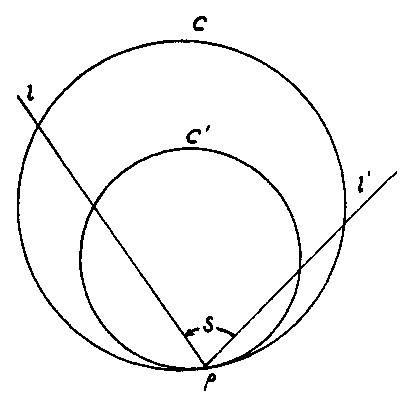
\includegraphics{chap05-vend-scan-01.eps}
\end{figure}

2. If $F(z)$ is a Poincar\'{e} series of dimension $-k$ with $k\geqq 5,\,F$ has a zero\index{Poincar\'{e} series!zeros of} at each parabolic vertex of $\Gamma$. [A parabolic sector $\mathscr{T}$ is made up of images of a finite number of sectors at the points of the cycle to which it belongs. Hence all isometric circles with a finite number of exceptions lie outside or on the boundary of $\mathscr{T}$, and for the centers $-d_{i}/c_{i}$ of these circles we have $|c_{i}z+d_{i}|\geqq 1$ for $z\in\mathscr{T}$. Therefore, as in the proof of Theorem 3A,
\begin{equation*}
|z-p|^{k}|F(z)| \leqq|z-p|^{k-4}\left\{|z-p|^{4}\sum\frac{|H(V_{i}z)|}{|c_{i}z+d_{i}|^{4}}\right\}+|z -p|^{k}A,
\end{equation*}
where $A$ is a finite sum, and the factor in braces is bounded as $z\rightarrow p$.]

3. If $f(z)$ is automorphic, $f^{\prime}(z)$ is a form of dimension $-2$.

4. Every automorphic function can be represented as the quotient of automorphic forms.

\section{The Valence of an Automorphic Function}\label{ch05:sec4}\index{automorphic function!valence of}\index{valence}

At this point we make an important restriction on the class of groups considered: \emph{the closed fundamental region} $\bar{R}$ \emph{meets} $\mathrm{Bd}\ \mathscr{D}$, \emph{if at all, only in parabolic vertices}. This implies $R$ has a finite number of sides. Cf. \ref{ch04:chap04}. \ref{ch04:sec4J}.

The fundamental result we are after is the following:

\begin{theorem*}
A nonconstant automorphic function assumes each value the same number of times in $R$.
\end{theorem*}

This number is called the \emph{valence} of the automorphic function. The proof will appear in 4H.

\subsection{}\label{ch05:sec4A}
First we have to define carefully what we mean by the order of\index{automorphic form!order of}\index{automorphic function!order of} a function at a point. We shall do this more generally for an automorphic form $F(z)$ of dimension $-k$. What we need are series expansions of $F$ at the points of $\mathscr{D}^{+}$.

We shall assume that $\infty$ is an ordinary point and is not a fixed point.

Let $z_{0}$ be a finite point of $\mathscr{D}$ which is not a fixed point. Define $t=z-z_{0}$ and $F(z)=\hat{F}(t)$. In a sufficiently small neighborhood of $z_{0}$ we have
\begin{equation}\label{ch05:eqn18}
F(z)=\hat{F}(t)=\sum\limits_{h=\mu}^{\infty}a_{h}t^{h},\qquad \mu\ \mathrm{finite},\qquad a_{\mu}\neq 0.
\end{equation}
We define $\mu$ to be the order of $F$ at $z_{0}$ and we write
\begin{equation*}
n(z_{0},\,F)=n(z_{0})=\mu.
\end{equation*}
If $\mu >0,\,F$ has a zero of order $\mu$ at $z_{0}$; if $\mu<0,\,F$ has a pole of order $-\mu$ at $z_{0}$. (When $z_{0}=\infty$, set $t=1/z$ and $F(z)=\hat{F}(t)$; define $n(\infty,\,F)=n(0,\,\hat{F})$.)

Next, suppose $z_{0}$ to be the (finite) fixed point of an elliptic transformation of order $l \geqq 2$. Let $z^{\prime}=Ez$ generate the subgroup $\Gamma_{z_{0}}$:
\begin{equation*}
\frac{z^{\prime}-z_{0}}{z^{\prime}-z_{0}^{\prime}}=\varepsilon\frac{z-z_{0}}{z-z_{0}^{\prime}},\qquad \varepsilon=e(1/l)
\end{equation*}
$z_{0}^{\prime}$ being the other (finite) fixed point of $E$. Differentiate logarithmically to get
\begin{equation*}
\frac{dE}{dz}=\frac{(z^{\prime}-z_{0})(z^{\prime}-z_{0}^{\prime})}{(z-z_{0})(z-z_{0}^{\prime})}=\varepsilon\bigg(\frac{z^{\prime}-z_{0}^{\prime}}{z-z_{0}^{\prime}}\bigg)^{2}.
\end{equation*}
Applying this and the transformation equation \eqref{ch05:eqn13} we find\footnote{Note that $(dE/dz)^{1/2}$ is single-valued: the case $k$ odd causes no difficulty.}
\begin{equation}\label{ch05:eqn19}
(z^{\prime}-z_{0}^{\prime})^{k}F(z^{\prime})=\varepsilon^{-m}(z-z_{0}^{\prime})^{k}F(z),\qquad m=k/2.
\end{equation}
Define
\begin{equation*}
t_{1}=\frac{z-z_{0}}{z-z_{0}^{\prime}},\qquad t_{1}^{\prime}=\frac{z^{\prime}-z_{0}}{z^{\prime}-z_{0}^{\prime}},
\end{equation*}
so that $t_{1}^{\prime}=\varepsilon\, t_{1}$. If we set
\begin{equation*}
G(t_{1})=(z-z_{0}^{\prime})^{k}F(z),
\end{equation*}
we can write \eqref{ch05:eqn19} in the form
\begin{equation*}
G(t_{1}^{\prime})=G(\varepsilon\, t_{1})=\varepsilon^{-m}G(t_{1}).
\end{equation*}

Clearly $G$ is meromorphic in a neighborhood of $t_{1}=0$, the point corresponding to $z=z_{0}$. Introduce the Laurent series,
\begin{equation*}
G(t_{1})=\sum\limits_{h=\mu_{1}}^{\infty}b_{h}t_{1}^{h},\qquad \mu_{1}\ \mathrm{finite}
\end{equation*}
into the above equation and get
\begin{equation*}
b_{h}(\varepsilon^{h+m}-1)=0.
\end{equation*}
It follows that only those coefficients survive for which $2h+k$ is a multiple of $2l$. This gives finally
\begin{equation}\label{ch05:eqn20}
(z-z_{0}^{\prime})^{k}F(z)=\hat{F}(t)=t^{-k/2l}\sum\limits_{h=\mu}^{\infty}a_{h}t^{h},\qquad \mu\ \mathrm{finite},\qquad a_{\mu}\neq 0
\end{equation}
where we have set
\begin{equation}\label{ch05:eqn21}
t =t_{1}^{l}=\left(\frac{z-z_{0}}{z-z_{0}^{\prime}}\right)^{l},\qquad G(t_{1})=\hat{F}(t)=(z-z^{\prime}_{0})^{k}F(z).
\end{equation}
The order of $F$ at $z_{0}$ is defined to be $\mu-k/2l$. (When $z_{0}=\infty$, this formula becomes
\begin{equation}\label{ch05:eqn22}
(z-z_{0}^{\prime})^{m}F(z)=\hat{F}(t)=\sum\limits_{\mu}^{\infty}a_{h}t^{h},\qquad t =1/(z-z_{0}^{\prime})^{l}.)
\end{equation}

We have already defined the order of $F$ at a parabolic point $z_{0}$ (cf. \eqref{ch05:eqn5}):
\begin{gather}\label{ch05:eqn23}
(z-z_{0})^{k}F(z)=\hat{F}(t)=\sum\limits_{h=\mu}^{\infty}a_{h}t^{h},\\
\nonumber t=e(1/c(z-z_{0})),\qquad\mu=n(z_{0},\,F).
\end{gather}
(If $z_{0}=\infty$, replace $1/(z-z_{0})$ by $z$ and define $F(z)=\hat{F}(t)$.)

Thus $n(z,\,F)$ is now defined for all $z\in \mathscr{D}^{+}$. The variable $t$ which occurs in the expansions \eqref{ch05:eqn18}, \eqref{ch05:eqn20}, and \eqref{ch05:eqn23} is called a \emph{local variable} or a \emph{local uniformizer}.


\subsection{}\label{ch05:sec4B}
In general $F$ has the same order at equivalent points. (An exception may occur when the points under consideration are equivalent to $\infty$.) In order to validate our assertion, we shall have to consider several cases. Let $z_{2}=Tz_{1}$. Set $\nu=n(z_{1},\,F)$. Assume neither $z_{1}$ nor $z_{2}$ is $\infty$.

1) $z_{1},\,z_{2}$ are ordinary points and not fixed points. We have given that $\lim_{z\rightarrow z_{1}}F(z)/(z-z_{1})^{\nu}=A$ exists and is not zero. Hence, with $w=Tz$, we get
\begin{equation*}
\lim_{w\rightarrow z_{2}}\frac{F(w)}{(w-z_{2})^{\nu}}=\left(\frac{dT}{dz}\right)_{z_{1}}^{-m}\lim_{z\rightarrow z_{1}}\left\{\left(\frac{z-z_{1}}{Tz-Tz_{1}}\right)^{\nu}\frac{F(z)}{(z-z_{1})^{\nu}}\right\}=\left(\frac{dT}{dz}\right)_{z_{1}}^{-m-\nu}\cdot A.
\end{equation*}
Therefore, the limit in the extreme left member exists and is not zero, for $(dT/dz)_{z_{1}}$ is infinite only at $T^{-1}(\infty)$ and is zero only at $\infty$.

2) $z_{1},\,z_{2}$ are elliptic fixed points of order $l$. Let $z_{1}^{\prime}, z_{2}^{\prime}$ be the conjugate fixed points. From \eqref{ch05:eqn20} we get, after a little calculation,
\begin{equation*}
\lim\limits_{t_{2}\rightarrow0} \frac{\hat{F}(t_{2})}{t_{2}^{\nu}}=\left(\frac{dT}{dz}\right)_{z_{1}}^{-m-\nu l}\left(\frac{z_{2}-z_{2}^{\prime}}{z_{1}-z_{1}^{\prime}}\right)^{k+\nu l} \lim\limits_{t_{1}\rightarrow0} \frac{\hat{F}(t_{1})}{t_{1}^{\nu}},
\end{equation*}
where $t_{1},\,t_{2}$ are the local variables at $z_{1}, z_{2}$ defined by \eqref{ch05:eqn21}. The result now follows by the same reasoning as before.

3) $z_{1},\,z_{2}$ are parabolic fixed points. The local variables are $t_{j}= e(1/c_{j}(z-z_{j})),\, j=1,2$, where
\begin{equation*}
P_{j}:\frac{1}{z^{\prime}-z_{j}}=\frac{1}{z-z_{j}}+c_{j}
\end{equation*}
is the generator of $\Gamma_{z_{i}}$. Now $P_{2}=TP_{1}T^{-1}$, and a calculation shows that $c_{2}=c_{1}/(dT/dz)_{z_{1}}$. Hence, as $z\rightarrow z_{1}$,
\begin{align*}
t_{2}&=e(1/c_{2}(Tz-Tz_{1}))\\
&=e\left\{\frac{1}{c_{1}}\left(\frac{dT}{dz}\right)_{z_{1}}\frac{1}{(dT/dz)_{z_{1}}\cdot(z-z_{1})+(d^{2}T/dz^{2})_{z_{1}}\cdot(z-z_{1})^{2}+\cdots}\right\}\\
&\sim\beta t_{1},\qquad \beta\neq0.
\end{align*}
We now have,
\begin{align*}
t_{2}^{-\nu}\hat{F}(t_{2})&=t_{2}^{-\nu}(Tz-Tz_{1})^{2m}F(Tz)=t_{2}^{-\nu}(Tz-Tz_{1})^{2m}(dT/dz)^{-m}F(z)\\
&\sim(\beta t_{1})^{-\nu}(dT/dz)^{m}\hat{F}(t_{1}),
\end{align*}
and the result follows. Hence:


\begin{lemma*}
If $z\neq\infty,\, Vz\neq\infty,\, V\in\Gamma$, then
\begin{equation*}
n(Vz,\,F)=n(z,\,F).
\end{equation*}
Also,
\begin{equation*}
n(V\infty,\,F)=n(\infty,\,F)-k,\qquad V\neq I.
\end{equation*}
\end{lemma*}

The second statement is proved by the same methods. Recall that $\infty$ (and therefore $V\infty$) is an ordinary point and not a fixed point.

\subsection{}\label{ch05:sec4C}
Let $F(z)$ be an automorphic form of dimension $-k$ which is not identically zero. We consider the problem of finding a formula for the sum $\sum n(z,\,F)$, where $z$ runs over a fundamental set of $\Gamma$ (a set which contains exactly one point from each equivalence class of $\Gamma$). By Lemma 4B this sum is independent of the particular fundamental set used provided it does not contain the point $\infty$.

Let $R_{i}=V_{i}(R)$, where $V_{i}\in\Gamma$. We shall construct a fundamental set $R_{i}^{\ast}$ by adding to $R_{i}$ the points on one side of each pair of congruent sides, and one vertex from each cycle of vertices.

Define
\begin{equation}\label{ch05:eqn24}
J_{i}(F)=J_{i}=\sum\limits_{z\in R_{t}^{\ast}}n(z,\,F),\qquad J= \sum\limits_{z\in R^{\ast}} n(z,\,F).
\end{equation}


\begin{theorem*}
$J_{n}(F)$ is finite. Moreover
\begin{gather*}
J_{n}(F)=J_{m}(F),\qquad V_{n}\neq I,\qquad V_{m}\neq I\\
J_{n}(F)=J(F)-k.
\end{gather*}
\end{theorem*}

The order $n(z,\,F)$ is different from $0$ only if $z$ is a zero or pole of $F$. Suppose, for example, there were infinitely many poles in $R_{n}$ accumulating at $z^{\ast}$, say. The point $z^{\ast}$ lies in $\bar{R}_{n}$ but also lies on the boundary of $\mathscr{D}$, for $F$ is meromorphic in $\mathscr{D}$. By virtue of our assumption at the beginning of this Section, $z^{\ast}$ is a parabolic vertex. But, as we saw in the opening lines of the proof of Theorem 1C, there can be only a finite number of poles in a parabolic sector. The number of poles of $F$ in $R_{n}^{\ast}$ is therefore finite; likewise the number of zeros. Hence $J_{n}<\infty$.

The second part of the theorem is an immediate consequence of Lemma 4B. $R_{n}$ and $R_{m}$ are bounded regions related by $R_{n}=V_{n}V_{m}^{-1}(R_{m})$. This gives the first equation. Also there is one point in $R_{n}$ equivalent to the point $\infty$ in $R$, whence the second equation.

From now on we restrict our attention to $J$. In general $J$ will not be an integer. For at an elliptic vertex the order of $F$ is not in general integral (cf. \eqref{ch05:eqn20}).

\subsection{}\label{ch05:sec4D}
The usual formula
\begin{equation*}
J=\frac{1}{2\pi i}\int_{S}\frac{F^{\prime}(z)}{F(z)}dz,
\end{equation*}
where $S$ is the boundary of $R$, must be modified to take account of the vertices, zeros, and poles lying on $S$. The modified contour $S^{\prime}$ and the region it bounds, $R^{\prime}$, are described as follows.

1) If $z_{1}$ is an interior point of a side $l$ at which $n(z_{1},\,F)\neq 0$, we make a small detour around $z_{1}$ lying in $R$ and the congruent detour around the equivalent point $z_{2}$ lying on the side congruent to $l$. The region $R^{\prime}$ includes $z_{2}$ but not $z_{1}$.

2) Let $z_{j},\,j=1,\,\cdots,\,s$ be the vertices of an accidental cycle. A small circle around $z_{1}$ can be divided into $s$ arcs which are congruent to arcs $C_{j}$ at $z_{j}$. The $\{C_{j}\}$ are the detours.

3) $z_{1},\,\cdots,\,z_{s}$ are the vertices of an elliptic or parabolic cycle. Choose for the detour around $z_{1}$ an arc of a fixed circle of the elliptic or parabolic substitution which generates the subgroup $\Gamma_{z_{1}}$. Draw corresponding detours $C_{j}$ around $z_{j}$ as in 2).

In each case we make the detours small enough so that they contain no zero or pole except the possible one at the point in question. Only a finite number of detours are required. Denote by $\beta_{j}$ the positive angle formed by the sides of $R$ meeting at $z_{j}$.

A word about the direction of integration. $R^{\prime}$ may not be simply connected or even connected. Then $S^{\prime}$ will consist of several pieces. We integrate along $S^{\prime}$ so that $R^{\prime}$ lies to the \emph{left}. This means, for example, that the detours $C_{j}$ will be described clockwise.

As a consequence of this construction we have
\begin{equation}\label{ch05:eqn25}
\frac{1}{2\pi i}\int_{S^{\prime}}\frac{F^{\prime}(z)}{F(z)}dz=\sum\limits_{z\epsilon R^{\prime}}n(z,\,F)+L,
\end{equation}
$L$ being the sum of the orders of $F$ at the \emph{inner} points of the sides of $R^{\prime}$.

The next step is to show that the contribution to the integral from the detours is just the sum of the orders of $F$ at the vertices.

1) \emph{Accidental cycle}. We may write $\nu=n(z,\,F),\,1\leqq j\leqq s$, the order being the same at each vertex (Lemma 4B). Then
\begin{equation*}
\frac{1}{2\pi i}\int_{C_{j}}\frac{F^{\prime}(z)}{F(z)}dz=\frac{1}{2\pi i}\int_{C_{j}}\left\{\frac{\nu}{z-z_{j}}+O(1)\right\}dz=-\frac{\nu\beta_{j}^{\prime}}{2\pi}+|C_{j}|\cdot O(1),
\end{equation*}
where $\beta_{j}^{\prime}$ is the positive angle through which the line $\overline{z_{j}z}$ turns as $z$ describes $C_{j}$, and $|C_{j}|$ is the euclidean length of $C_{j}$. If we let $C_{j}$ shrink to $z_{j}$, we have $\beta_{j}^{\prime}\rightarrow\beta_{j}$ and $|C_{j}|\rightarrow 0$; hence
\begin{equation*}
\frac{1}{2\pi i}\int_{C_{j}}\frac{F^{\prime}(z)}{F(z)}dz=\frac{-\nu\beta_{j}}{2\pi}+o(1).
\end{equation*}

\begin{figure}[!h]
\includegraphics{chap05-vend-scan-02.eps}
\end{figure}

\noindent Now $\sum\nolimits_{j=1}^{s}\beta_{j}=2\pi$ (\ref{ch04:chap04}. Th.~\ref{ch04:sec4C}), so
\begin{equation*}
\sum\limits_{j=1}^{s}\frac{1}{2\pi i}\int_{C_{j}}\,\frac{F^{\prime}(z)}{F(z)}dz=-\nu+o(1).
\end{equation*}
2) \emph{Elliptic cycle of order} $l$. Here we have (cf. \eqref{ch05:eqn20}),
\begin{equation*}
\frac{F^{\prime}(z)}{F(z)}dz=-\frac{k}{z-z_{j}^{\prime}} dz+ \frac{\hat{F}^{\prime}(t)}{\hat{F}(t)}dt,\qquad j=1, 2,\,\cdots,\,s
\end{equation*}
with $z_{j}^{\prime}$ the fixed point conjugate to $z_{j}$ and $t$ defined by \eqref{ch05:eqn21}. Now $t$ maps $C_{j}$ on an arc $K_{j}$ of a circle about the origin in the $t$-plane. The arc subtends an angle $l\beta_{j}$ and is described in the same sense as $C_{j}$. Hence with $\nu=n(z_{j},\,F),\,1\leqq j\leqq s$,
\begin{equation*}
\sum\limits_{j=1}^{s}\frac{1}{2\pi i}\int_{C_{j}}\frac{F^{\prime}(z)}{F(z)}dz=-\sum\limits_{j=1}^{s}\frac{\nu l\beta_{j}}{2\pi}+o(1)=-\nu+o(1),
\end{equation*}
since $\sum\nolimits_{j=1}^{s}\,\beta_{j}=2\pi/l$.

4) \emph{Parabolic cycle}. The arc $C_{j}$ is mapped onto an arc $C_{j}^{\prime}$ lying on the fixed circle of which $C_{1}$ is a part by a transformation $T_{j}^{-1}=(\cdot\,\cdot|c_{j}\,d_{j}),\,1\leqq j\leqq s;\,T_{1}=I$. The arcs $\{C_{j}^{\prime}\}$ fit together to make up an arc that is mapped, without change of sense, into a full circle $K$ in the $t$-plane by the function $t=e(1/c(w-z_{1}))$. For $2\leqq j\leqq s$, we get, using \eqref{ch05:eqn1} and \eqref{ch05:eqn23},
\begin{align*}
\int_{C_{j}}\,\frac{F^{\prime}(z)}{F(z)}dz&=\int_{C_{j}}d\log F(z)=\int_{C_{j}^{\prime}} d\log F(T_{j}w)\\
&=2m\int_{C_{j}^{\prime}}\frac{dw}{w+d_{j}/c_{j}}+\int_{C_{j}^{\prime}}d\log F(w)\\
&=2m\int_{C_{j}^{\prime}}\left\{\frac{1}{w+d_{j}/c_{j}}-\frac{1}{w-z_{1}}\right\}dw-\int_{K_{j}}\frac{\hat{F}^{\prime}(t)}{\hat{F}(t)}dt,
\end{align*}
$K_{j}$ being the image of $C_{j}^{\prime}$ in the $t$-plane. As the radius of $C_{j}^{\prime}$ tends to $0$, the first integral in the right member approaches $0$, for the angle subtended by $C_{j}^{\prime}$ vanishes in the limit (cf. Note 10, p. 401). Thus
\begin{equation*}
\int_{C_{j}}\frac{F^{\prime}(z)}{F(z)}dz=o(1)-\int_{K_{j}}\frac{\hat{F}^{\prime}(t)}{\hat{F}(t)}dt,\qquad j=2,\,3,\,\cdots,\,s.
\end{equation*}
Since the result is the same when $j=1$, the term $1/(w+d_{1}/c_{1})$ being absent, we now have
\begin{equation*}
\sum\limits_{j=1}^{s}\frac{1}{2\pi i}\int_{C_{j}}\frac{F^{\prime}(z)}{F(z)}dz=-\frac{1}{2\pi i}\int_{K}\, \frac{\hat{F}^{\prime}(t)}{\hat{F}(t)}dt +o(1)=-\nu+o(1).
\end{equation*}

Collecting these results we have
\begin{equation*}
-\sum n(z,\,F)=\frac{1}{2\pi i}\int\frac{F^{\prime}(z)}{F(z)}dz+o(1),
\end{equation*}
the sum being over a set of inequivalent vertices in $R$ and the integral being over the union of the detours. If we now combine this with \eqref{ch05:eqn25} and let the detours shrink to their points, we obtain
\begin{equation}\label{ch05:eqn26}
\sum\limits_{z\in R^{\ast}}n(z,\,F)=\frac{1}{2\pi i}\sum\limits_{i=-n}^{n}\int_{s_{i}}\frac{F^{\prime}(z)}{F(z)}dz,
\end{equation}
where we have enumerated the sides of $R^{\ast}$ in conjugate pairs $(s_{1},\,s_{-1}),\,\cdots,\, (s_{n},\,s_{-n})$.


\subsection{}\label{ch05:sec4E}
Let $V_{i}(s_{i})=s_{-i}$. If $V_{i}=(\cdot\cdot|c_{i}\,d_{i})$, the point $-d_{i}/c_{i}$ is the center of\index{automorphic form!order of} the isometric circle $\Im(V_{i})$. Recall that the image of $s_{i}$ under $V_{i}$ is directed oppositely to $s_{-i}$. Hence
\begin{equation*}
\int_{s_{-i}}\frac{F^{\prime}(z)}{F(z)}dz=-\int_{s_{i}}\frac{F^{\prime}(V_{i}w)}{F(V_{i}w)}d\,V_{i}w=-2m\int_{s_{i}}\frac{dw}{w+d_{i}/c_{i}}-\int_{s_{i}}\, \frac{F^{\prime}(w)}{F(w)}dw,
\end{equation*}
or
\begin{equation*}
\int_{s_{-i}}+\int_{s_{i}}\left(\frac{F^{\prime}}{F}dz\right)=-2m\int_{s_{i}}\frac{dw}{w+d_{i}/c_{i}}=2m\alpha_{i},
\end{equation*}
where $\alpha_{i}$ is the angle subtended by the arc $s_{i}$ at the center of the isometric circle on which it lies. Since the angle subtended by $s_{\,\mbox{-}i}$ is also $\alpha_{i}$, we can sum over all the sides of $R$ to get
\begin{equation*}
\sideset{}{^{\prime}}\sum\limits_{i=-n}^{n}\frac{1}{2\pi i}\int_{s_{i}}\frac{F^{\prime}}{F}dz=\frac{m}{2\pi}\sideset{}{^{\prime}}\sum\limits_{i=-n}^{n}\alpha_{i},
\end{equation*}
where $\sum\nolimits^{\prime}$ means $i\neq 0$ in the summation.

With \eqref{ch05:eqn26} this completes the proof of the following


\begin{theorem*}
Let $F(z)$ be a nonidentically vanishing automorphic form of dimension $-k$ on $\Gamma$. Then
\begin{equation}\label{ch05:eqn27}
J=\sum\limits_{z\in R^{\ast}}n(z,\,F)=\frac{m}{2\pi}\sideset{}{^{\prime}}\sum\limits_{i=-n}^{n}\alpha_{i}.
\end{equation}
\end{theorem*}

\subsection{}\label{ch05:sec4F}
An important corollary of the last theorem is the following:


\begin{theorem*}
If $f$ is an automorphic function, $f\not\equiv 0$,
\begin{equation*}
J(f)=\sum\limits_{z\in R^{\ast}}n(z,f)=0.
\end{equation*}
\end{theorem*}

This result\footnote{For two forms $F,\,G$ of the same dimension we have $J(F/G)=J(F)-J(G)=0$, since $F/G$ is a \emph{function}. This shows that $J$ depends only on the dimension, not on the particular form $F$, as we observe in \eqref{ch05:eqn27}.} states that $f$ has as many zeros as poles\index{automorphic function!zeros and poles} in $R^{\ast}$, counted according to the conventions we have laid down.



\subsection{}\label{ch05:sec4G}
The number of poles of $f$ in $R_{i}^{\ast}$ is independent of $i$ and is equal to the number of poles in $R^{\ast}$, by Lemma 4B. This number is called the \emph{valence} of $f$ and is denoted by $N(f)$. According to Theorem 4C it is finite.


\begin{theorem*}
If $f$ is nonconstant, $N(f)>0$. Or, an automorphic function regular\index{automorphic function!a regular \_\_\_is constant} in the closed fundamental region is a constant.
\end{theorem*}

Suppose $f$ is pole-free in $R^{\ast}$. Let $z_{0}$ be a point of $R$. The function $g(z)=f(z) -f(z_{0})$ is automorphic and has a zero\index{automorphic function!zeros and poles} at $z=z_{0}$. By the preceding result, $g\equiv 0$. Hence $f(z)\equiv f(z_{0})$.

\subsection{}\label{ch05:sec4H}
We are now able to prove the fundamental theorem announced at the beginning of this Section.


\begin{theorem*}
A nonconstant automorphic function\index{automorphic function!valence of} $f$ assumes each complex value $N(f)$ times in any fundamental set $R_{i}^{\ast}$.
\end{theorem*}

Since $f$ is not constant, $N(f)$ is positive. Now $f-c$ is automorphic and has $N(f)$ poles in $R_{i}^{\ast}$; it therefore has $N(f)$ zeros. But a zero of $f-c$ is a point where $f$ assumes the value $c$.\:\:\:q.e.d.

This theorem shows that an automorphic function is completely determined by the principal parts of its expansions at the poles in $R^{\ast}$ and its value at one point. For the difference of two functions with the same principal parts is regular in $R^{\ast}$ and so is a constant.

These conclusions were proved on the basis that $\infty$ is neither a limit point nor a fixed point. If this is not the case, $\Gamma^{\prime}=A\Gamma A^{-1}$ has the desired property for a certain linear transformation $A$. Let $R^{\prime}$ be the standard fundamental region of $\Gamma^{\prime};R=A^{-1}(R^{\prime})$ is then a fundamental region for $\Gamma$. Consider the function $g(z)=f(A^{-1}z)$, where $f$ is the given automorphic function on $\Gamma$. As we have seen (Theorem 3D), $g$ is automorphic on $\Gamma^{\prime}$. Now
\begin{equation*}
n(Az,\,g)=n(z,f),\qquad z\in R
\end{equation*}
as can be proved by the arguments used for Lemma 4B. It follows that Theorems 4G and 4H hold for $f$ since they hold for $g$. Cf. Note 11, p. 401.

\subsection{}\label{ch05:sec4I}
We have seen that a nonconstant automorphic function has a positive valence. The lowest possible valence is 1. Are there functions of valence 1, that is, functions which assume each value once in the fundamental region? This depends entirely on the group $\Gamma$ and, in fact, on a topological characteristic of $\Gamma$ called the genus. We shall see in the next chapter (\ref{ch06:chap06}. Th. \ref{ch06:sec2K}) that groups of genus $0$\index{group of genus 0}, and only those groups, support univalent functions.


\subsection{}\label{ch05:sec4J}
\begin{theorem*}
An automorphic form of positive dimension\index{automorphic forms of positive dimension} $(k<0)$ which is regular at each point of $R^{\ast}$ vanishes identically.
\end{theorem*}


Recalling that $k=2m$, we have $m<0$. Hence $J<0$ (Theorem 4E). Thus there are more poles than zeros, so there must be at least one pole.

\subsection{}\label{ch05:sec4K}
When $\Gamma$ is a principal-circle group, equation \eqref{ch05:eqn27} takes a more interesting and significant form. Suppose $\Gamma$ is horocyclic and is defined on\footnote{$\mathscr{U}$ is the unit disk.} $\mathscr{U}$. The fundamental region $R_{0}$ is the intersection of $R$ and $\mathscr{U}$; hence
\begin{equation*}
\tag{$^{\ast}$} J_{0}=\frac{m}{2\pi}\sum\limits_{i=-n}^{n}{^{\prime}}\alpha_{i},
\end{equation*}
where $J_{0}$ denotes the sum of the orders of\index{automorphic form!order of} the automorphic form $F$ in the fundamental set constructed from $R_{0}$.

$R_{0}$ is a polygon since we are assuming it has a finite number of
sides

\begin{figure}[!h]
\includegraphics{chap05-vend-scan-03.eps}
\end{figure}

(\ref{ch04:chap04}. Th. \ref{ch04:sec6F}). If $l$ is the order of an elliptic
cycle, $2\pi/l$ is the sum of the angles in $R_{0}$ at the vertices
of the cycle. We can include accidental and parabolic cycles in this
formula by setting $l=1$ for the former and $1/l=0$ for the latter.
Thus $2\pi\sum 1/l$ is the sum of the interior angles of the polygon
$R_{0}$.

Suppose $R_{0}$ has $2n$ sides. We now construct a straight-sided polygon $P$ of $4n$ sides by joining the endpoints of each side to the center of the isometric circle on which it lies (cf. Figure). The interior angles of $P$ consist of the angles $\alpha_{i}$, the angles at the vertices, and the angles $\gamma_{i}$ and $\delta_{i}$. The latter are each $\pi/2$. Hence
\begin{equation*}
(4n-2)\pi=\sum\,\alpha_{i}+2\pi\sum\, 1/l_{i}+2n\pi,
\end{equation*}
and so from $(^{\ast})$,
\begin{equation}\label{ch05:eqn28}
J_{0}=m(n-1-\sum\,1/l_{i}),
\end{equation}
the sum being extended over all cycles of $R_{0}$. This formula was found by \citeauthor{Poincare0000}\index{Poincar\'{e}} ([\ref{Poincare1}, p. 195]).

In Chapter~\ref{ch06:chap06} we shall define a topological invariant of $\Gamma$, the \emph{genus} $g$, which is computed from the formula
\begin{equation*}
c\,-n+1=2-2g,
\end{equation*}
where $c$ is the number of cycles. Substituting this in \eqref{ch05:eqn28} gives a relation between $g$ and $J_{0}$:
\begin{equation}\label{ch05:eqn29}
J_{0}=k\left\{g-1+\frac{1}{2}\sum\left(1-\frac{1}{l_{i}}\right)\right\}.
\end{equation}
The expression in braces is proportional to the noneuclidean area of the fundamental region $R_{0}$. Cf. Ex. 5-2.

This formula is also correct for groups of the second kind (not horocyclic).


\skiptoctrue
\section*{Exercise}

1. Let $G$ be an automorphic form of dimension $-2m$ on $\Gamma$, and let the element $E \in\Gamma$ have distinct fixed points $z_{0},\,z_{0}^{\prime}$. Then $f(z) =(z-z_{0})^{m}\times (z-z_{0}^{\prime})^{m}G(z)$ is invariant on the cyclic group generated by $E$.

\section{Principal-Circle Groups}\label{ch05:sec5}\index{principal-circle group}

\subsection{}\label{ch05:sec5A}
If $\Gamma$ is a principal-circle group, all of the preceding developments apply, of course. But we can get better results by taking advantage of the hyperbolic geometry which can be defined in this case.

Since all disks and half-planes are conformally equivalent, we shall normalize to the unit disk $\mathscr{U}:|z|<1$, and its boundary $\mathscr{Q}:|z|=1$. In this section $\Gamma$ shall denote a group discontinuous in $\mathscr{U}$. The disk $\mathscr{U}$ serves as a model of the hyperbolic plane. The relevant hyperbolic concepts (line, distance, $\cdots$) will be denoted by the prefix $H$. They have been discussed in \ref{ch02:chap02}. \ref{ch02:sec12}. The $H$-elements of length and area, for example, are
\begin{equation*}
\frac{d\rho}{1-\rho^{2}},\,\frac{\rho\,d\rho\,d\theta}{(1-\rho^{2})^{2}}
\end{equation*}
respectively, where $z=\rho e^{i\theta}$. They are invariant under conformal homeomorphisms of $\mathscr{U}$.

The substitutions of $\Gamma$ are of the form
\begin{equation*}
V_{i}=\left(\begin{matrix}
a_{i} & \bar{c}_{i}\\c_{i} & \bar{a}_{i}
\end{matrix}\right),\quad a_{i}\bar{a}_{i}-c_{i}\bar{c}_{i}=1,\quad i=0,1,\cdots;\qquad V_{0}=I.
\end{equation*}
Recall also that $\infty$ is an ordinary point, and if $\infty$ is a fixed point, it is fixed by only a finite number of substitutions. In this section we permit $\infty$ to be a fixed point. The fundamental region $R_{0}$ is the intersection of $R$ with $\mathscr{U}$---cf. \ref{ch04:chap04}. \ref{ch04:sec5A}.


\subsection{}\label{ch05:sec5B}
For the present class of groups we can prove the convergence of the Poincar\'{e} series when $r >2$ and not only when $r \geqq 4$. The proof is a sort of noneuclidean version of the one in 2B.

Define
\begin{equation*}
J_{\alpha}=\iint\limits_{K}\frac{\rho d\rho\,d\theta}{(1-\rho^{2})^{\alpha}},
\end{equation*}
an integral that converges when $\alpha<1$. Let $K_{0}$ be a small disk lying within $R_{0}$ and let $K_{i}=V_{i}(K_{0})$. The $K_{i}$ are mutually disjoint. It follows that
\begin{equation*}
\sum\limits_{i}\iint\limits_{K_{i}}\frac{\rho\,d\rho\,d\theta}{(1-\rho^{2})^{\alpha}}<J_{\alpha}<\infty,\ \alpha<1.
\end{equation*}

In each integral of this sum we make the change of variable $z=V_{i}w,\,z =\rho \exp i\theta,\,w=\rho^{\prime}\exp i\theta^{\prime}$. Using the invariance of the area element and the easily verified formula
\begin{equation}\label{ch05:eqn30}
1-|V_{i}w|^{2}=(1-|w|^{2})|c_{i}w+\bar{a}_{i}|^{-2},
\end{equation}
we get
\begin{align*}
J_{\alpha}&>\sum\limits_{i}\iint\limits_{K_{0}}\frac{1}{(1-|V_{i}w|^{2})^{\alpha-2}}\frac{\rho^{\prime}d\rho^{\prime}d\theta^{\prime}}{(1-\rho^{\prime2})^{2}}\\
&=\sum\limits_{i}\iint\limits_{K_{0}}\frac{\rho^{\prime}d\rho^{\prime}\,d\theta^{\prime}}{(1-\rho^{\prime 2})^{\alpha}|c_{i}w+\bar{a}_{i}|^{4-2\alpha}}.
\end{align*}

Let $\sum^{\ast}$ be the sum over those terms (all but a finite number) for which $c_{i}\neq 0$. Since $\infty$ is an ordinary point and $a_{i}/c_{i}=V_{i}\infty$, we conclude that $|a_{i}/c_{i}|$ is bounded for $V_{i}$ in $\sum\nolimits^{\ast}$. Hence, setting $4-2\alpha=r$, we get
\begin{equation*}
J_{\alpha}>\sum\nolimits^{\ast}\frac{1}{|c_{i}|^{r}}\iint\limits_{K_{0}}\frac{\rho^{\prime}\,d\rho^{\prime}\,d\theta^{\prime}}{(1-\rho^{\prime 2})^{\alpha}(|w|+|\bar{a}_{i}/c_{i}|)^{r}}>M\,\sum\nolimits^{\ast}\frac{1}{|c_{i}|^{r}},
\end{equation*}
where $M$ is a positive constant. Now $\alpha<1$ is equivalent to $r>2$, and so we have the desired result:


\begin{theorem*}
If $r>2$,
\begin{equation*}
\sum\nolimits{^{\ast}}|c_{i}|^{-r}
\end{equation*}
converges.
\end{theorem*}

\subsection{}\label{ch05:sec5C}
By arguments entirely analogous to those of Sections 2 and 3, we can now prove the following theorem.


\begin{theorem*}
Let $H(z)$ be a rational function having no poles in $\mathscr{L}$. When $k\geqq3$ the Poincar\'{e} series\index{Poincar\'{e} series!convergence of} \eqref{ch05:eqn12},
\begin{equation*}
F(z)=\sum\limits_{i=0}^{\infty}H(V_{i}z)(c_{i}z+\bar{a}_{i})^{-k},
\end{equation*}
converges absolutely uniformly\footnote{This means the series of absolute values converges uniformly.} on the sets $S_{1}$ described in Theorem \emph{2D}. $F$ is an automorphic form of dimension $-k$.
\end{theorem*}

If $\Gamma$ is horocyclic, i.e., $\Gamma$ is not discontinuous on $\mathscr{Q}$, the Poincar\'{e} series defines two functions, $F_{1}(z)$ meromorphic inside $\mathscr{Q}, F_{2}(z)$ meromorphic outside $\mathscr{Q}$. Each function has the transformation property \eqref{ch05:eqn1} in its respective region. If $\Gamma$ is not horocyclic, its domain of existence $\mathscr{D}$ includes both the interior and exterior of $\mathscr{Q}$ and certain arcs on $\mathscr{Q}$. The Poincar\'{e} series then defines a single function $F(z)$, which is meromorphic in $\mathscr{D}$.

\subsection{}\label{ch05:sec5D}
We mentioned without proof in 2H that the Poincar\'{e} series\index{Poincar\'{e} series!convergence of} of dimension $-2$ diverges when $\Gamma$ is horocyclic and converges in the contrary case. We shall now give the demonstration. The proof for horocyclic $\Gamma$ is a recent one by \citeauthor{Lehner0000}~[\ref{Lehner5}]\index{Lehner, J.}.


\begin{theorem*}
If $\Gamma$ is a principal-circle group and is not horocyclic, then
\begin{equation*}
\sum\nolimits^{\ast}|c_{i}|^{-2}<\infty.
\end{equation*}
\end{theorem*}

Let $\sigma_{0}$ be an arc of $\mathscr{Q}$ lying entirely in the interior of the fundamental region $R_{0}$. Then $V_{i}\sigma_{0}=\sigma_{i}$ lies in $R_{i}\cap \mathscr{Q}$ and is disjoint from $\sigma_{j}(i\neq j)$. Denoting by $|\sigma_{i}|$ the euclidean length of $\sigma_{i}$, we obviously have
\begin{equation*}
\sum\limits_{i=0}^{\infty}|\sigma_{i}|\leqq 2\pi.
\end{equation*}
Now
\begin{equation*}
|\sigma_{i}|=\int_{\sigma_{i}}|d\zeta|=\int_{\sigma_{0}}|V^{\prime}(z)|\,|dz|=\int_{\sigma_{0}}|c_{i^{Z}}+\bar{a}_{i}|^{-2}|dz|.
\end{equation*}
Hence when $c_{i}\neq 0$ we get, with $M$ an upper bound for $|\bar{a}_{i}/c_{i}|$,
\begin{gather*}
|\sigma_{i}|\,\geqq|c_{i}|^{-2}(1+M)^{-2}|\sigma_{0}|,\\
\sum{^{\ast}}|c_{i}|^{-2}\leqq(1+M)^{2}|\sigma_{0}|^{-1}\sum{^{\ast}}|\sigma_{i}|<\infty.\ \mathrm{q.e.d.}
\end{gather*}

\subsection{}\label{ch05:sec5E}
Suppose now $\Gamma$ is horocyclic \emph{and has a fundamental region with a finite number of sides}. Suppose
\begin{equation*}
\tag{$^{\ast}$} \sum|c_{i} z+\bar{a}_{i}|^{-2}<\infty
\end{equation*}
for some $z=z_{0}\in \mathscr{U}$. The ratio $|c_{i} z_{0}+\bar{a}_{i}|/|c_{i}z+\bar{a}_{i}|$ is bounded above for $z\in \mathscr{U}$, since $|\bar{a}_{i}/c_{i}|$ is bounded above and below. Hence $(^{\ast})$ converges for all $z$ in $\mathscr{U}$. Using \eqref{ch05:eqn30} we deduce that
\begin{equation}\label{ch05:eqn31}
\sum(1-|V_{i}z|^{2})<\infty.
\end{equation}

Define the Blaschke product\index{Blaschke product}
\begin{equation}\label{ch05:eqn32}
\pi(z)=\prod_{n=0}^{\infty}\frac{z-z_{n}}{\bar{z}_{n}z-1}e^{-i\beta_{n}},
\end{equation}
where
\begin{equation*}
z_{n}=V_{n}^{-1}(0),\qquad \beta_{n}=\arg z_{n}.
\end{equation*}


\begin{lemma*}
The product \eqref{ch05:eqn32} converges uniformly in $|z|\leqq \rho <1$ whenever \eqref{ch05:eqn31} holds. The product
\begin{equation}\label{ch05:eqn33}
\prod_{n=0}^{\infty}\left|\frac{z-z_{n}}{\bar{z}_{n}z-1}\right|
\end{equation}
converges absolutely\footnote{The product $\Pi(1+a_{n})$ is said to converge absolutely if $\Pi(1\,+|a_{n}|)$ converges.} in $\mathscr{U}$. \emph{Cf. Note 12}.
\end{lemma*}

Denote the factors of \eqref{ch05:eqn32} by
\begin{equation*}
u_{n}=f_{n}e^{i_{\varphi_{n}}},\qquad f_{n}=f_{n}(z)\geqq 0
\end{equation*}
and set $U_{N}=u_{1}u_{2}\cdots u_{N} =F_{N}\exp i\Phi_{N}$. Since $u_{n}$ is a conformal homeomorphism of $\mathscr{U}$ and $|z_{n}|<1$, we have $f_{n}<1$. Hence $1-f_{n}<1-f_{n}^{2}$. Calculation shows that
\begin{equation*}
1-f_{n}^{2}=(1-|z|^{2})(1-|z_{n}|^{2})|\bar{z}_{n}z-1|^{-2}.
\end{equation*}
Since $|\bar{z}_{n}z-1|\geqq 1 -|z|$, this gives
\begin{equation*}
\sum|1-f_{n}|\leqq 2(1\,-|z|\,)^{-1}\sum(1-|z_{n}|^{2}),
\end{equation*}
and we have seen that the series in the right member converges. Thus $F_{N}(z)$ converges uniformly in $|z|\leqq\rho <1$, since\footnote{Recall that the product $\Pi\{1+a_{n}(z)\}$ converges uniformly in any region where $\sum |a_{n}(z)|$ converges uniformly.} $F_{N}=f_{1}f_{2}\cdots f_{N}$.

Next,
\begin{equation*}
\varphi_{n}=\arg u_{n}=\arg\frac{z-z_{n}}{\bar{z}_{n}\overline {}z-1}-\arg z_{n}=\arg\frac{z-z_{n}}{|z_{n}|^{2}z-z_{n}}.
\end{equation*}
As $n\rightarrow\infty,\,|z_{n}|\rightarrow1$. It is not hard to show by means of a diagram that $|\varphi_{n}|\,|z-z_{n}|\sim|z|(1-|z_{n}|^{2})$. For $n>N,\,|z_{n}|>(1+\rho)/2$ and so $|\varphi_{n}|< 2\rho(1-|z_{n}|^{2})/(1-\rho)$ when $|z|\leqq \rho$. Hence $ \Phi_{N}=\sum\nolimits_{n=1}^{N}\varphi_{n}$ converges uniformly in $|z|\leqq \rho$ as $N\rightarrow\infty$. This proves the first statement of the lemma. The second is equivalent to the convergence of $\sum (1-f_{n})$, which we have already established.

From the lemma we deduce that $\pi(z)$ is regular in $\mathscr{U}$, and obviously $|\pi(z)|\leqq 1$. Moreover, we may rearrange the order of the factors of the product \eqref{ch05:eqn33}. Now
\begin{equation*}
\left|\frac{z-z_{n}}{\bar{z}_{n}z-1}\right|=|V_{n}z|.
\end{equation*}
Hence, for $L\in\Gamma$,
\begin{equation*}
|\pi(Lz)|=\prod_{n=0}^{\infty}|V_{n}Lz|=|\pi(z)|,
\end{equation*}
since $V_{n}L$ runs with $V_{n}$ over the matrices of $\Gamma$.

The function $\pi(z)$ vanishes exactly on the set $\{z_{n}\}$. Let
\begin{equation*}
\mathscr{B}=\mathscr{U}-\{z_{n}\}.
\end{equation*}
Since $0<|\pi(z)|\leqq 1$ in $\mathscr{B}$, we can define a unique branch of
\begin{equation*}
\varphi(z)=\log|\pi(z)|,
\end{equation*}
$\varphi$ is harmonic in $\mathscr{B}$ and
\begin{equation*}
\varphi(z)\leqq 0.
\end{equation*}
Moreover,
\begin{equation*}
\varphi(Vz)=\varphi(z),\qquad V\in\Gamma.
\end{equation*}

Furthermore it is known that $\pi(z)$, as a Blaschke product, possesses radial limits of absolute value 1 almost everywhere (\citeauthor{Nevanlinna0000}~[\ref{Nevanlinna2}\index{Nevanlinn}, p. 196]). Hence
\begin{equation*}
w(\zeta)=\lim_{r\rightarrow 1}\varphi(r\zeta)=0
\end{equation*}
for almost all $\zeta$ on $\mathscr{Q}$. \emph{The function} $\varphi$ \emph{is a} $\Gamma$-\emph{invariant nonpositive harmonic function in}\index{harmonic function}\index{invariant harmonic function} $\mathscr{B}$ \emph{and its radial limits vanish almost everywhere},

\subsection{}\label{ch05:sec5F}
We now proceed as follows. Suppose $\bar{R}_{0}$ is contained in a disk $|z|\leqq \rho<1$. Let $\zeta_{0}$ be such that $\omega(\zeta_{0})=0$ and let $\zeta_{n}\rightarrow \zeta_{0}$ on the radius $\arg\zeta_{0}$. We may also assume that the radius $O\zeta_{0}$ lies in $\mathscr{B}$, i.e., avoids the countable set $\{z_{n}\}$. Each $\zeta_{n}$ has a $\Gamma$-image $\zeta_{n}^{\prime}$ lying in $\bar{R}_{0}$, i.e., $|\zeta_{n}^{\prime}|\leqq\rho$. Let $\zeta_{p}^{\prime}$ be a subsequence converging to $\zeta^{\ast},\,|\zeta^{\ast}|\leqq \rho$. Since $\varphi(\zeta_{p})\rightarrow 0$, we have, because of the invariance, $\varphi(\zeta_{p}^{\prime})\rightarrow 0$. Now $\zeta^{\ast}\not\in\{z_{n}\}$, for $\varphi(z)\rightarrow-\infty$ as $z \rightarrow z_{n}$. Hence $\zeta^{\ast}\in \mathscr{B},\,\varphi$ is continuous at $\zeta^{\ast}$, and $\varphi(\zeta^{\ast})=0$. The function $\varphi$ assumes its maximum at $\zeta^{\ast}$, an interior point of $\mathscr{B}$, and so is a constant. But $\varphi$ is no constant, for it becomes infinite at $z_{n}$. Thus we have proved the desired result for the case of compact $\bar{R}_{0}$:


\begin{theorem*}
Let $\Gamma$ be horocyclic and have a fundamental region with a finite number of sides. Then the Poincar\'{e} series\index{Poincar\'{e} series!divergence of} $\sum|c_{i}z+\bar{a}_{i}|^{-2}$ diverges.
\end{theorem*}

\subsection{}\label{ch05:sec5G}
When $R_{0}$ has vertices on $\mathscr{Q}$ the method fails, for the images $\zeta_{n}^{\prime}$ may tend to the vertices. To get around the difficulty we shall make use of a geometrical theorem that has many other applications.


\begin{theorem*}
Let $\Gamma$ be a principal-circle group, horocyclic or not, defined on $\mathcal{U}$ and having a fundamental region with a finite number of sides. Let $\zeta_{0}\in \mathscr{Q}$ be a limit point of $\Gamma$ and not a parabolic vertex. If $\lambda\in \mathscr{U}$ is a circular arc orthogonal to $\mathscr{Q}$ and ending at $\zeta_{0}$, there is a number $\rho$, depending only on $\Gamma,\,0<\rho <1$, a sequence of points $\zeta_{n}$ on $\lambda$ tending to $\zeta_{0}$, and $\Gamma$-images $\zeta_{n}^{\prime}=V_{n}\zeta$, such that
\begin{equation*}
|\zeta_{n}^{\prime}|\leqq \rho.
\end{equation*}
\end{theorem*}

In the proof we shall assume $\lambda$ is the radius $O\zeta_{0}$. This is permissible, for the distance from the circular arc to the radius tends to $0$ as we approach $\mathscr{Q}$ (cf. Ex. 5-3). The asymptotic properties of the two curves are therefore identical.

The proof for horocyclic $\Gamma$ is due to \citeauthor{Hedlund0000}\index{Hedlund}\index{Hedlund's lemma} ([\ref{Hedlund1}, p. 538]).

Suppose $\Gamma$ is horocyclic. If there are no parabolic vertices, the result is obvious, for the fundamental region $\bar{R}_{0}$ is compact with respect to $\mathscr{U}$ and contains, on the other hand, an image of every point on $\lambda$. Assume, then, there are parabolic vertices. A horocycle $C(p,\,r)$ is a euclidean circle of radius $r<1$ tangent to $\mathscr{Q}$ at $p$. Let $p_{1},\,p_{2},\,\cdots,\,p_{s}$ be the parabolic vertices of $R_{0}$. Since $R_{0}$ has a finite number of sides, $s$ is finite. Draw horocycles $C_{i}=C(p_{i},\,r_{i}),\,i=1,2,\,\cdots,\,s$, so that the union of their interiors covers $R_{0}$. This can be done by taking $r_{i}$ near enough to 1.

Let $P_{i}$ be a parabolic element of $\Gamma$ generating the subgroup of $\Gamma$ that fixes $p_{i}$. Then $C_{i}$ is invariant under $P_{i}$. If $z_{0}$ is any point on $C_{i}$ different from $p_{i}$, there are two images of $z$ on $C_{i}$ whose euclidean distances from the origin are minimal. Call these images $z_{1}$ and $z_{2}$ and call the larger of the two distances $d_{i}$. The arc $z_{1}z_{2}$ is mapped by the powers of $P_{i}$ into a family of arcs which cover $C_{i}-p_{i}$ once and only once. Hence every point $z$ on $C_{i}$ except $p_{i}$ has a $\Gamma$-image $z^{\prime}$ lying in $z_{1}z_{2}$, so the distance from $z^{\prime}$ to the origin is not more than $d_{i}$. Set $\rho=\max(d_{1},\,d_{2},\, \cdots,\,d_{s})$. Then $\rho<1$, and every point of any of the horocycles $C_{i}$ except a point of tangency has an image lying in the disk $|z|\leqq \rho$.

Let $\mathbf{C}$ be the set of horocycles $\{C_{i},\,i=\,1,\,\cdots ,s\}$ together with all their images under $\Gamma$. Every point of $\mathscr{U}$ is interior to some member of the set $\mathbf{C}$. Let $a\neq\zeta_{0}$ be an arbitrary point on $\lambda$. We assert the segment $a\zeta_{0}$ meets horocycles of $\mathbf{C}$. Otherwise $a\zeta_{0}$ lies entirely in one horocycle and $\zeta_{0}$ is a parabolic vertex, contrary to the assumption. It is now evident that $\lambda$ meets infinitely many horocycles in points $\zeta_{n}\rightarrow\zeta_{0}$. By what has been proved, each $\zeta_{n}$ has a $\Gamma$-image in the disk $|z|\leqq \rho$.

The argument has to be modified slightly if $\Gamma$ is not horocyclic. Then $R_{0}$ will have free sides. The region formed by a free side, the sides meeting the free side, and an arc of a circle concentric with $\mathscr{Q}$ and cutting both (inner) sides, is called a \emph{funnel} (cf. Figure (a)). Recall that a free side of $R_{0}$ adjoins other free sides (of other fundamental regions) at each endpoint. Clearly if the height of a funnel is small enough, any radius that enters a funnel must leave it by its free side or by an adjacent free side (cf. Figure (b)) Draw a funnel $F_{i}$ at each free side $f_{i},\,i=1,\,\cdots,\,t$, satisfying this condition. Denote by $\mathbf{F}$ the set of funnels together with all their images under $\Gamma$.

\begin{figure}[!h]
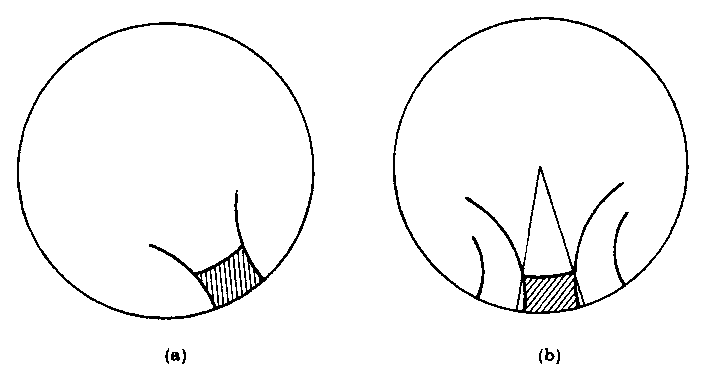
\includegraphics{chap05-vend-scan-04.eps}
\end{figure}

Suppose there are no parabolic vertices. Let $a\neq\zeta_{0}$ be an arbitrary point on $\lambda$. The point $a$ cannot lie in a member of $\mathbf{F}$, for this would imply that $\zeta_{0}$ is a point of a free side and so is no limit point. Thus $a$ is equivalent to a point of $\bar{R}_{0}-\bigcup_{i=1}^{t}F_{i}$, a compact subset of $\mathscr{U}$, and the theorem is evident. We therefore assume there are parabolic vertices.

As before we construct a horocycle $C_{i}$ at each parabolic vertex $p_{i},1\leqq i\leqq s$, lying in $R_{0}$. We shall make $C_{i}$ large enough so $\bigcup_{i=1}^{s}\,\mathrm{Int}\,C_{i}$ covers $R_{0}-\bigcup_{i=1}^{t}F_{i}$. Let $\mathbf{C}$ be the same set as before. As a consequence of this construction we can assert that every point of $\mathscr{U}$ lies in a member of $\mathbf{C}$ or a member of $\mathbf{F}$.

For the same reason as before the point $a\in\lambda,\,a\neq\zeta_{0}$, cannot lie in a member of $\mathbf{F}$. Hence $a$ lies in an element of $\mathbf{C}$ and the argument goes through as in the previous case. This completes the proof.

\subsection{}\label{ch05:sec5H}
We can now\index{Poincar\'{e} series!divergence of} prove Theorem 5F in the case of noncompact $R_{0}$. Consider the function $\varphi$ discussed in 5E. Since $\varphi(z)$ has the radial limit zero almost everywhere, and since for a horocyclic group $\mathscr{L}=\mathscr{Q}$, there must be a $\zeta_{0} \in\mathscr{L}$ that is not in the countable set $\mathscr{P}$ and such that $\varphi(r\zeta_{0})\rightarrow 0$ with $r\rightarrow 1$. If $\zeta_{n},\,\zeta_{n}^{\prime}$ are the sequences of Theorem 5G, we have $\varphi(\zeta_{p}^{\prime})\rightarrow 0$ and $\zeta_{p}\rightarrow\zeta^{\ast}$ with $|\zeta^{\ast}|\leqq \rho <1$. The remainder of the proof is the same as in 5F.


\subsection{}\label{ch05:sec5I}
We can use the above developments to get a short proof, at least for horocyclic groups, of the fundamental Theorem 4G, that an automorphic function regular\index{automorphic function!a regular\_\_\_is constant} and bounded in the fundamental region is a constant. The idea was first used for the modular group by \citeauthor{Rademacher0000}~[\ref{Rademacher11}]\index{Rademacher} and then generalized by \citeauthor{Lehner0000}~[\ref{Lehner5}]\index{Lehner, J.}.

Let $\Gamma$ be horocyclic; then the series $\sum |c_{i}z+\bar{a}_{i}|^{-2}$ diverges. We may assume $z_{n}=V_{n}^{-1}(0)$ different from $0$ for $n\geqq N$. Using \eqref{ch05:eqn30} we see that the divergence of the above series at $z=0$ implies the divergence of $ \sum\nolimits_{n=N}^{\infty}(1-|z_{n}|)$. This is equivalent to
\begin{equation*}
\tag{$^{\ast}$} \prod_{n=N}^{\infty}|z_{n}|=0.
\end{equation*}

Let $f(z)$ be automorphic on $\Gamma$ and bounded in $\mathscr{U}$. If $f$ is not constant, there is an integer $k$ so that
\begin{equation*}
g(z)=\frac{f(z)-f(0)}{z^{k}}
\end{equation*}
has the property $g(0)\neq 0$. The function $g$ is regular and bounded in $\mathscr{U}$ and is not identically zero. For $z_{n}\neq 0$ we have $g(z_{n})=0$ by virtue of
\begin{equation*}
f(z_{n})=f(V_{n}^{-1}(0))=f(0).
\end{equation*}

We now apply


\textsc{Jensen's Inequality}. \emph{Let $g(z)$ be\index{Jensen's inequality} regular and $|g(z)|\leqq M$ in $|z|\leqq R$, let $g(0)\neq 0$, and let $g(z_{n})=0,\,n=1,2,\,\cdots,\,s$ with $|z_{n}|<R$. \emph{(}$g$ may also vanish at points other than $z_{n}$.\emph{)} Then}
\begin{equation*}
|z_{1}z_{2}\cdots z_{s}|\geqq|g(0)|/M.
\end{equation*}
(Cf. [\citeauthor{Bieberbach0000}~\ref{Bieberbach1}\index{Bieberbach}, p. 109].) Hence
\begin{equation*}
|z_{N}z_{N+1}\cdots z_{m}|\geqq|g(0)|/M,
\end{equation*}
for each $m\geqq N$, where $M>0$ is the upper bound of $|g(z)|$ in $\mathscr{U}$. Because of $(^{\ast})$ this involves $g(0)=0$. Hence there is no integer $k$ and $f$ is constant.

\subsection{}\label{ch05:sec5J}
We close this section with two examples. The first is a Poincar\'{e} series\index{Poincar\'{e} series!identical vanishing of} whose sum is identically zero. Let $\Gamma$ be a group containing an elliptic substitution of order $n\geqq 2$,
\begin{equation*}
T:\frac{z^{\prime}-\alpha}{z^{\prime}-\alpha^{\prime}}=e\left(\frac{1}{n}\right)\cdot\frac{z-\alpha}{z-\alpha^{\prime}},
\end{equation*}
where $|\alpha|<1$ and $\alpha^{\prime}=1/\bar{\alpha}$. Let $G$ be the finite group generated by $T$ and write the coset decomposition $\Gamma=\bigcup_{i} GW_{i}$.

Define $H(z)=(z-\alpha^{\prime})^{-2n-2}$. The Poincar\'{e} series,
\begin{equation*}
F(z)=\sum\limits_{V\in\Gamma}H(Vz)(cz+\bar{a})^{-2n-2},
\end{equation*}
converges. Note that if $V=T^{j}W_{l}$,
\begin{align*}
(cz\,+\bar{a})^{-2}&=\frac{dT^{j}W_{l}z}{dz}=\frac{dT^{j}W_{l}z}{dW_{l}z}\cdot\frac{dW_{l}z}{dz}\\
&=e\left(\frac{j}{n}\right)\cdot\left(\frac{T^{j} W_{l}z-\alpha^{\prime}}{W_{l}z-\alpha^{\prime}}\right)^{2}\cdot\frac{dW_{l}z}{dz}\cdot
\end{align*}
(Cf. equation preceding \eqref{ch05:eqn19}.) Hence
\begin{equation*}
F(z)=\sum\limits_{l=0}^{\infty}\left(\frac{dW_{l}z}{dz}\right)^{n+1}\frac{1}{(W_{l}z-\alpha^{\prime})^{2n+2}}\sum\limits_{j=0}^{n-1}e\left(\frac{j(n+1)}{n}\right),
\end{equation*}
where the interchange of order is justified by absolute convergence. Since $n$ does not divide $n+1$ when $n>1$, the inner sum equals $0$. Hence $F(z)\equiv 0$.

\subsection{}\label{ch05:sec5K}
The second example is a Poincar\'{e} series\index{Poincar\'{e} series!everywhere regular}, not identically zero, which is regular throughout $\mathscr{U}$. Let $\Gamma$ be a group devoid of elliptic elements. Then no point of $\mathscr{U}$ is a fixed point. For convenience assume $-I\in\Gamma$. Consider the series
\begin{equation*}
F_{k}(z)= \sum\limits_{V\in\ \Gamma}(cz+\bar{a})^{-2k},\qquad V=\left(\begin{matrix}a&\bar{c}\\c&\bar{a}\end{matrix}\right),\qquad k=\mathrm{integer}.
\end{equation*}
For $k>1$ the series converges uniformly and defines $F_{k}$ as a regular function in $\mathscr{U}$, as we have seen. We shall show that $F_{k}\not\equiv 0$ if $k$ is sufficiently large.

Note that if $V\neq\pm I$ then $c \neq 0$, otherwise $z =0$ would be a fixed point. Hence $a\bar{a}>1$ for all such $V$, since $a\bar{a}-c\bar{c}=1$. We assert that the series $\sum|a|^{-2k}$, extended over all $V\neq\pm I$, converges uniformly with respect to $k$ for $k\geqq 2$. Indeed, $|a|^{-2k}\leqq|a|^{-4}\leqq|c|^{-4}$, and $ \sum|c|^{-4}$ converges by Theorem 5B. It follows that $\sum\bar{a}^{-2k}$ converges uniformly in the same range of $k$. Therefore,
\begin{equation*}
\lim\limits_{k\rightarrow\infty}\sum\limits_{V\in\Gamma}\bar{a}^{-2k}=\sum\limits_{V\in\Gamma}=\lim\limits_{k\rightarrow\infty}\overline{a}^{-2k}=\sum\limits_{V=\pm l}+\sum\limits_{V\neq\pm l}=2+0.
\end{equation*}
For sufficiently large $k$ we have $F_{k}(0)=\sum\bar{a}^{-2k}\neq 0$ and so $F_{k}(z)\not\equiv 0$.


\skiptoctrue
\section*{Exercises}

1. A triangle lying in $\overline{\mathscr{U}}$ or $\overline{\mathscr{H}}$ whose sides are $H$-lines has $H$-area equal to $\pi$ minus the sum of its interior angles. [The expression for the area is a double integral which can be converted by Green's Theorem into a line integral along the boundary of the triangle. The calculation of the line integral is conveniently made in $\mathscr{H}$.]

2. Let $\Gamma$ be\index{fundamental region!hyperbolic area} horocyclic and have a fundamental region $R_{0}$ with a finite number of sides. If $g$ is defined by the formula in the lines preceding \eqref{ch05:eqn29}, the $H$-area of $R_{0}$ equals
\begin{equation*}
4\pi\left\{g-1+\frac{1}{2}\sum\,\left(1-\frac{1}{l_{i}}\right)\right\},
\end{equation*}
the sum being taken over the cycles of $R_{0}$. (Recall that $1/l_{i}$ is $0$ for a parabolic cycle, 1 for an accidental cycle.) In particular, if $\Gamma$ consists entirely of hyperbolic transformations, the area is $4\pi(g-1)$. [Triangulate $R_{0}$ by drawing lines from the origin to its vertices and calculate its $H$-area from the preceding exercise. Combine this with the definition of $g$.]

3. Let $\lambda$ be an $H$-segment ending at $\alpha\in \mathscr{Q}$. Show that the perpendicular $H$-distance from the point $z$ on $\lambda$ to the radius $O\alpha$ tends to $0$ as $z \rightarrow\alpha$. [Transform to the upper half-plane]

\section{Algebraic and Differential Relations}\label{ch05:sec6}

\subsection{}\label{ch05:sec6A}
The reader is familiar with special cases of the theorem we are about to prove. The equation $\sin^{2} z +\cos^{2}z=1$ is an algebraic equation connecting $\sin z$ and $\cos z$, two automorphic functions on the simply-periodic group. (Note that $|\sin z|$ tends to a definite limit, $\infty$, as $z \rightarrow\infty$ within a period strip, i.e., fundamental region) Another example is
\begin{equation*}
J(\tau)=\frac{4}{27}\frac{(1-\lambda+\lambda^{2})^{3}}{\lambda^{2}(1-\lambda)^{2}},\qquad  \lambda=\lambda(\tau)
\end{equation*}
where $J$ is automorphic on the modular group $\Gamma(1)$ and $\lambda$ is automorphic on $\Gamma(2)$, the principal congruence subgroup of order 2. Cf. \ref{ch01:chap01}. \ref{ch01:sec1E}.


\begin{theorem*}
Let $\Gamma$ be a discontinuous function group satisfying the condition of Section \emph{4}. If $f,\,g$ are automorphic functions on $\Gamma$, they satisfy an algebraic equation\index{automorphic function!algebraic equation satisfied by}
\begin{equation*}
P(f,\,g)=0
\end{equation*}
with complex coefficients.
\end{theorem*}

Let
\begin{equation*}
\Phi(z)=\sum\limits_{i=0}^{s}\sum\limits_{j=0}^{t}a_{ij}f^{i}(z)g^{j}(z),
\end{equation*}
with arbitrary complex $a_{ij}$ and arbitrary integers $s,\,t$. $\Phi$ is automorphic on $\Gamma$. We shall show that constants $a_{ij}$ can be chosen so that $\Phi$ has more zeros than poles in a fundamental region. According to Theorem 4F, $\Phi$ vanishes identically; whence, the theorem.

Suppose $f$ has $n$ poles, $g$ has $m$ poles, in $R$, counted in correct multiplicity. Then for $N(\Phi)$, the total number of poles of $\Phi$, we have the inequality,
\begin{equation*}
N(\Phi)\leqq ns+mt.
\end{equation*}

There are $(s+1)(t+1)=\nu+1$ constants in $\Phi$. Select $\nu$ points $z_{1},\,\cdots,\,z_{\nu}$ in, $R$ that are distinct from each other and from the poles of $f$ and $g$. The conditions $\Phi(z_{1})=\cdots=\Phi(z_{\nu})=0$ are equivalent to $\nu$ linear equations in $\nu+1$ variables $\{a_{ij}\}$, which therefore always have a nontrivial solution. The polynomial $\Phi$ formed with such constants has at least $\nu$ zeros in $R$. For $s$ and $t$ sufficiently large
\begin{equation}\label{ch05:eqn34}
\nu=(s+1)(t+1)-1>ns+mt.\qquad \mathrm{q.e.d}.
\end{equation}

\subsection{}\label{ch05:sec6B}
Suppose $f$ is univalent\index{automorphic function!univalent} in $R$, i.e., $n=1$. Then \eqref{ch05:eqn34} is satisfied\index{automorphic function!algebraic equation satisfied by} for $s=m,\,t=1$. Hence
\begin{equation*}
gQ_{1}(f)+Q_{2}(f)=0,
\end{equation*}
where $Q_{1},\,Q_{2}$ are polynomials. If $Q_{1}\equiv 0$ we would have $Q_{2}(f)\equiv 0$, which implies that $f$ assumes only a finite number of values, namely, the zeros of $Q_{2}$. Hence $Q_{1}\not\equiv 0$ and we get
\begin{equation*}
g=-Q_{2}(f)/Q_{1}(f).
\end{equation*}


\begin{theorem*}
If there is a univalent function $f$ on $\Gamma$, every automorphic function is a rational function of $f$.
\end{theorem*}

\subsection{}\label{ch05:sec6C}
The set of automorphic functions on $\Gamma$ is obviously a field\index{automorphic function!field of\_\_\_s}, which we denote by $\mathbf{K}(\Gamma)$. The last theorem states that in certain cases $\mathbf{K}$ is isomorphic to a field of rational functions of a single variable. \emph{It is always true that} $\mathbf{K}(\Gamma)$ \emph{is isomorphic to a field of algebraic functions of one variable}. We shall prove this noteworthy result in the next chapter (\ref{ch06:chap06}. \ref{ch06:sec5C}), and in the course of the argument a new proof of Theorem 6A will appear. It must be stressed that Theorems 6A--6C are not true for groups whose fundamental regions have an infinite number of sides. Nor are they true if we relax the condition that an automorphic function be meromorphic at the parabolic vertices in the sense in which we have defined the term. For then $\exp f(z)$ would be automorphic if $f$ is automorphic according to our definition. The two restrictions we have made, one on the group, the other on the functions, are absolutely essential if the field of automorphic functions is to be an algebraic function field.


\subsection{}\label{ch05:sec6D}
The derivative\index{Schwarzian derivative} of\index{automorphic form!derivatives of} an automorphic function is a form of dimension $-2$. More generally we have the following result:


\begin{theorem*}
If $F$ is a form of dimension $-k$, then
\begin{equation*}
\Phi_{k}=kFF^{\prime\prime}-\,(k+1)F^{\prime 2}
\end{equation*}
is a form of dimension $-2k -4$. Here $\Gamma$ is an arbitrary discontinuous function group.
\end{theorem*}

The proof of the required invariance property is a straightforward verification beginning with the square of the transformation formula:
\begin{equation*}
F^{2}(Vz)=(cz+d)^{2k}F^{2}(z),\qquad V\in\Gamma.
\end{equation*}
Clearly $\Phi_{k}$ is meromorphic at ordinary points of $\Gamma$. At a parabolic vertex $p$ we have
\begin{equation*}
F(z)=Q(t)R(z),\qquad t=e(1/c(z\,-p))
\end{equation*}
where $R$ is a rational function of $z$ and $Q(t)$ is a power series in $t$. It is easily seen that any derivative of $F$ has the same form and hence also $\Phi_{k}$. Then $\Phi_{k}$ tends to a definite limit as $z\rightarrow p$ within a parabolic sector. Thus $\Phi_{k}$ is meromorphic at the parabolic vertices and the proof is complete.

As an immediate consequence we have:

\begin{corollary*}
Define the ``Schwarzian derivative''
\begin{equation}\label{ch05:eqn35}
D(w)_{z}=\frac{2w^{\prime}w^{\prime\prime\prime}-3(w^{\prime\prime})^{2}}{2w^{\prime 2}},\qquad w=w(z).
\end{equation}
If $w(z)$ is automorphic on $\Gamma$, so is
\begin{equation*}
\varphi(z)=\frac{D(w)_{z}}{w^{\prime}(z)^{2}}.
\end{equation*}
\end{corollary*}

Take $k=2$ and $F=w^{\prime}$; then the numerator of $D(w)_{z}$ is a form of dimension $-8$.

\subsection{}\label{ch05:sec6E}
Poincar\'{e}\index{Poincar\'{e}} used the Schwarzian derivative to prove the following


\begin{theorem*}
Assume $\Gamma$ is a function group satisfying the restriction of Section 4. Let $w(z)$ be a nonconstant automorphic function and let $z =\zeta(w)$ be the inverse function. Then
\begin{equation*}
z=\frac{\eta_{1}(w)}{\eta_{2}(w)},
\end{equation*}
where $\eta_{1},\,\eta_{2}$ satisfy a linear differential equation\index{differential equations}
\begin{equation*}
\frac{d^{2}\eta}{dw^{2}}=A(w)\eta,
\end{equation*}
in which $A$ is an algebraic function of $w$.
\end{theorem*}

Define
\begin{equation*}
\tag{$^{\ast}$} \eta_{1}(w)=z\cdot(w^{\prime})^{1/2},\qquad\eta_{2}(w)=(w^{\prime})^{1/2},\qquad w^{\prime}=dw/dz
\end{equation*}
the square root being fixed at a point where the derivative is not $0$. We show that $\eta_{1},\,\eta_{2}$ satisfy the differential equation.

From $(^{\ast}$) we get
\begin{equation*}
\tag{$^{\ast\ast}$} w^{\prime}=\eta_{1}^{2}z^{-2}=\eta_{2}^{2},
\end{equation*}
and we can use this equation to calculate $w^{\prime\prime},\,w^{\prime\prime\prime}$ and hence $D(w)_{z}$. The result is
\begin{equation*}
D(w)_{z}=2z^{-4}\eta_{1}^{3}\frac{d^{2}\eta_{1}}{dw^{2}}=2\eta_{2}^{3}\frac{d^{2}\eta_{2}}{dw^{2}},
\end{equation*}
and this with $(^{\ast\ast})$ gives
\begin{equation*}
\frac{1}{\eta_{1}}\frac{d^{2}\eta_{1}}{dw^{2}}=\frac{1}{\eta_{2}}\frac{d^{2}\eta_{2}}{dw^{2}}=\frac{D(w)_{z}}{2w^{\prime2}}=\frac{1}{2}\varphi(z).
\end{equation*}
In Corollary \ref{ch05:sec6D} we proved that $\varphi$ is automorphic on $\Gamma$; hence, from Theorem 6A, it is an algebraic function of $w,\,1/2\varphi(z)=A(w)$. Thus $\eta_{1},\,\eta_{2}$ are solutions of $\eta^{\prime\prime}=A\eta$ and by $(^{\ast}$), $z=\eta_{1}/\eta_{2}$.\:\:\:q.e.d.

If $w$ is univalent, $A$ is a rational function.

\skiptoctrue
\section*{Exercise}

1. Prove:
\begin{equation*}
D\left(\frac{aw+b}{cw+d}\right)_{z}=D(w)_{z}.
\end{equation*}

2. Let $F(z)$ be an automorphic\index{Schwarzian derivative} form of positive dimension $s$. Then $d^{(s+1)}F(z)/dz^{s+1}$ is a form of dimension $-s-2$.


%%%%%%%%%chapter06

\chapter{Riemann Surfaces}\label{ch06:chap06}

Felix Klein\index{Klein, F.}, a deep student of the works of Riemann\index{Riemann}, constructed the theory of automorphic functions from Riemann's theorems of existence of functions on Riemann surfaces. In this chapter we shall give an exposition of this development.

We shall have to assume some familiarity with the Riemann surface, as a complete exposition would be a book in itself. However, we have included a sketch of the theory, so that the uninitiated reader who is willing to take certain things on faith can still follow the developments of this chapter. Complete details can be found in standard texts on Riemann surfaces. Several new ones have appeared in the last ten years, for example, \citeauthor{Ahlfors0000a}\index{Ahlfors-Sario} [\ref{Ahlfors}], \citeauthor{Nevanlinna0000}~[\ref{Nevanlinna1}]\index{Nevanlinn}, \citeauthor{Pfluger0000}~[\ref{Pfluger1}]\index{Pfl\"{u}ger}, \citeauthor{Springer0000}~[\ref{Springer1}].\index{Springer}

From an independent theory of automorphic functions, such as we have presented in the two preceding chapters, it is possible to derive the theory of Riemann surfaces as orbit spaces of plane domains by discontinuous groups. The two theories are thus essentially equivalent.

\section{Riemann Surfaces}\label{ch06:sec1}\index{Riemann surface}

\subsection{}\label{ch06:sec1A} A Riemann surface is a 2-dimensional manifold with directly conformal neighbor relations\index{neighbor relation}. In detail this means the following. Let $S$ be a connected Hausdorff space (\ref{ch02:chap02}. \ref{ch02:sec2A}. \ref{ch02:sec2I}). Let $S$ be covered by a collection of open sets $\{U_{i}\}$ each of which is homeomorphic to an open subset of the euclidean plane. Let
\begin{equation}
\label{ch01:eqn1a} t_{i}=\Phi_{i}(q),\qquad q\in U_{i}
\end{equation}
be the homeomorphism ; $\Phi_{i}$ assigns a coordinate to each point of $U_{i}$, namely, the complex number $t_{i}$. If $U_{i}$ and $U_{j}$ meet in a set $D$, each point of $D$ has two coordinates, $t_{i}$ and $t_{j}$. The function $\varphi(t)=\Phi_{j}\circ\Phi_{i}^{-1}(t)$ maps $\Phi_{i}(D)$ on $\Phi_{j}(D)$. $\varphi$ is called a \emph{neighbor relation}; it is a complex-valued function of the complex variable $t$ and is a 1-1 mapping since it is the composition of homeomorphisms. We demand further that $\varphi(t)$ be directly conformal on its domain.

We now make a formal definition\index{Riemann surface!definition}.

\begin{definition*} Let $S$ be a connected Hausdorff space. Let $U=\{U_{i}\}$ be an open covering of $S$ and let $\Phi=\{\Phi_{i}\}$, where $\Phi_{i}$ is a homeomorphism of $U_{i}$ onto an open subset of the euclidean plane. Then $S$ is called a Riemann surface provided,

1) for $\Phi_{i},\,\Phi_{j}\in\Phi$, the composition $\Phi_{i}\circ\Phi_{j}^{-1}$, when it is defined, is directly conformal on its domain.

The pair $(U,\, \Phi)$ is said to define an \emph{analytic structure}\index{analytic structure} on $S$. Another pair ($V,\, \Psi),\,V=\{V_{i}\},\,\Psi=\{\Psi_{i}\}$, defines the same structure provided the pair $(U\cup V,\, \Phi \cup\Psi)$ satisfies
1).
\end{definition*}

\subsection{}\label{ch06:sec1B} Each set $U_{i}$ containing the point $q\in S$ is called a \emph{parametric neighborhood} of $q$ and the variable $t_{i}$ of (\ref{ch01:eqn1a}) is called a \emph{local variable}\index{local variable} or \emph{local uniformizer}\index{local uniformizer} at $q$ or of $U_{i}$. In particular, if $\Phi_{i}(U_{i})$ is a euclidean disk $K,\,U_{i}$ is termed a \emph{parametric disk}\index{parametric disk}. Let $t^{\ast}$ be the center of $K$; then $q^{\ast}=\Phi_{i}^{-1}(t^{\ast})$ is called the \emph{center} of $U_{i}$. It is not hard to show that \emph{each} $q\in S$ \emph{is the center of a parametric disk}.

Moreover, any pair of local variables $t,\,\tau$ of a point $q$ are related by an equation of the form
\begin{equation}
\label{ch01:eqn2b} t-t_{0}=\alpha_{1}(\tau-\tau_{0})+\alpha_{2}(\tau-\tau_{0})^{2}+\cdots,\quad\alpha_{1}\neq 0,\, t_{0}=t(q),\,\tau_{0}=\tau(q).
\end{equation}
For if $t=\Phi_{i}(p), \tau =\Phi_{j}(p)$, then
\begin{equation*}
t=\Phi_{i}\circ\Phi_{j}^{-1}\circ\Phi_{j}(p)=\Phi_{i}\circ\Phi_{j}^{-1}(\tau),
\end{equation*}
and $\Phi_{i} \circ\Phi_{j}^{-1}$ is directly conformal by condition 1) of the definition in~\ref{ch06:sec1A}. Since it is also 1-1 and since $t=t_{0}$ when $\tau = \tau_{0}$, equation (\ref{ch01:eqn2b}) follows (\ref{ch02:chap02}. \ref{ch02:sec8A}).

A local uniformizer defines a coordinate system in its parametric neighborhood. A different uniformizer may assign different coordinates, but the transition from one coordinate system to another is made by a conformal transformation. For the calculation of a local conformally invariant quantity, any coordinate system may be used provided it holds in a neighborhood of the point in question. By the same token it is natural to define on a Riemann surface only those concepts which are conformally invariant.


\subsection{}\label{ch06:sec1C} The notion of orientation is familiar for the plane as is the fact that directly conformal mappings are orientation-preserving. We therefore define a manifold $M$ to be \emph{orientable}\index{Riemann surface!is orientable} provided there is a covering of $M$ by parametric neighborhoods $U_{i}$ and corresponding homeomorphisms $\Phi_{i}$ such that all neighbor relations $\Phi_{i}\circ\Phi_{j}^{-1}$ are orientation-preserving mappings. It follows that \emph{every Riemann surface is orientable}, for the neighbor relations are required to be directly conformal.


\subsection{}\label{ch06:sec1D} If a Riemann surface considered as a topological space is compact, it is called a \emph{compact}\index{Riemann surface!compact} or \emph{closed} surface; in the contrary case, a \emph{noncompact} or \emph{open} surface. It is a fundamental result of surface topology that every compact orientable 2-dimensional manifold is topologically equivalent to a sphere with a finite number of handles (\citeauthor{Springer0000}~[\ref{Springer1},\index{Springer} p. 124]). \emph{The number of handles is called} the \emph{genus}\index{compact Riemann surface!genus of}\index{Riemann surface!genus of} and is denoted by $g$. If $g=0$ the surface is a sphere; if $g=1$ it is a torus, etc. Thus every compact Riemann surface is a surface of genus $g$ for some nonnegative integer $g$.


\subsection{}\label{ch06:sec1E} A Riemann surface can be \emph{triangulated}\index{Riemann surface!triangulation of}. It is intuitively clear what we would mean by a triangulation of a surface like a sphere or a region of the plane. To extend the idea to a Riemann surface $S$ (in fact, to any manifold), we make the following definition: the homeomorphic image in $S$ of a euclidean triangle is called a \emph{triangle in} $S$ provided it lies entirely within a parametric disk. Let $\Delta=\{S_{i}\}$ be a collection of triangles in $S$. We say $\Delta$ is a \emph{triangulation of} $S$ if
\begin{enumerate}
\item[1)] each point of $S$ lies in at least one triangle of $\Delta$
\item[2)] two triangles meet, if at all, in a common vertex or a common edge
\item[3)] each point of $S$ has a neighborhood meeting only finitely many triangles.
\end{enumerate}

\emph{A triangulation of a compact} $S$ \emph{contains only a finite number of triangles}. Otherwise, the set $\{q_{i}\}$, where $q_{i}\in \mathrm{Int}\, S_{i}$, has by compactness a point of accumulation $q^{\ast}$ in $S$, but $q^{\ast}$ has no neighborhood of the type demanded by 3).

That every Riemann surface can be triangulated is a rather deep result (\citeauthor{Springer0000}~[\ref{Springer1},\index{Springer} p. 239]). But as we have mentioned, a \emph{compact} surface $S$ is topologically equivalent to $S_{g}$, a sphere with $g$ handles, and we can see directly that $S_{g}$ can be triangulated. The mapping of $S_{g}$ onto $S$ then induces a triangulation on $S$.


\subsection{}\label{ch06:sec1F} The genus\index{Riemann surface!genus of} of $S$ can be computed by Euler's formula from the data of the triangulation:
\begin{equation}
\label{ch06:eqn3} \alpha_{0}-\alpha_{1}+\alpha_{2}=2-2g,
\end{equation}
where $\alpha_{0}$ is the number of vertices, $\alpha_{1}$ the number of edges, and $\alpha_{2}$ the number of triangles. The genus is a topological invariant; in particular, it does not depend on the triangulation used.

Sometimes $S$ is mapped topologically on a plane polygon in which certain sides, vertices, are identified. In such cases \eqref{ch06:eqn3} is still valid provided we count two identified sides as one side, etc.


\subsection{}\label{ch06:sec1G} The pictorial model of a Riemann surface as discussed in texts on function theory is a many-sheeted surface lying over the complex plane. The rigorous formulation of this concept is the \emph{covering surface}.


\begin{definition*} Let $\tilde{S}$ be a manifold (\ref{ch02:chap02}.~\ref{ch06:sec3K}) and $\pi$ a mapping (projection) of $\tilde{S}$ into a Riemann surface $S$. Then the pair $(\tilde{S},\,\pi)$ is said to be a smooth\index{covering surface!smooth} covering surface of $S$ provided each $\tilde{q}_{0}\in\tilde{S}$ has a neighborhood $\tilde{V}$ which is mapped topologically by $\pi$ onto a neighborhood $V$ of $q_{0}=\pi(\tilde{q}_{0})$. The condition implies that $\pi$ is continuous. We say that $\tilde{q}\in\tilde{S}$ lies over $q\in S$ provided $\pi(\tilde{q})=q$. The covering surface is called unlimited if, for every arc $\gamma$ in $S$ with initial point $q$ and for every point $\tilde{q}$ in $\tilde{S}$ lying above $q$, there is an arc $\bar{\gamma}$ in $\tilde{S}$ with initial point $\tilde{q}$ which lies above $\gamma$. (An arc is a continuous image of the closed interval $[0,\,1]$.)

The analytic structure of $S$ can be \emph{lifted} to $\tilde{S}$ by noticing that $t\circ\pi$ is a local variable at $\tilde{q}_{0}$ if $t$ is a local variable at $\pi(\tilde{q}_{0})$. Thus $\tilde{S}$ becomes a Riemann surface.
\end{definition*}

\subsection{}\label{ch06:sec1H} In general $S$ will have many different smooth covering surfaces $\{\tilde{S}_{i},\,\pi_{i}\}$. A partial ordering (\ref{ch02:chap02}.~\ref{ch06:sec1C}) can be introduced into the family of coverings by defining $(\tilde{S}_{1},\,\pi_{1})<(\tilde{S}_{2},\, \pi_{2})$ if and only if $(\tilde{S}_{2},\,\pi_{2})$ is a smooth covering of $(\tilde{S}_{1},\, \pi_{1})$ by a projection $\varphi$ satisfying $\pi_{1}\circ\varphi =\pi_{2}$. Under this ordering $\{\tilde{S}_{i},\, \pi_{i}\}$ is not only a \emph{lattice} but it contains a largest element, called the \emph{universal covering surface}\index{universal covering surface} and denoted by $\hat{S}$. The universal covering surface of $S$, then, covers every covering surface of $S$. Its principal property is that it is \emph{simply connected}. (A Riemann surface is simply connected if every simple closed curve (homeomorph of a circle) lying in the surface can be shrunk to a point.)


\subsection{}\label{ch06:sec1I} Let $(\tilde{S},\,\pi)$ be a smooth unlimited covering of $S$.
A \emph{covering transformation}\index{covering transformation} $h$ of $(\tilde{S},\,\pi)$ is a homeomorphism of $\tilde{S}$ onto itself such that a point and its image have the same projection in $S$, i.e., $\pi \circ h=\pi$. The transformation $h$ is completely determined by specifying $h(\tilde{q})$ for a single point $\tilde{q}$ on $\tilde{S}$. Hence no covering transformation has a fixed point except the identity.

The set of covering transformations obviously forms a group $H(\tilde{S})$. This group is said to be \emph{transitive} provided that for any two points $\tilde{q}_{1},\,\tilde{q}_{2}$ with the same projection there is an $h\in H$ such that $h(\tilde{q}_{1})=\tilde{q}_{2}$. The group $H(\hat{S})$ is always transitive.


\subsection{}\label{ch06:sec1J} The pictorial Riemann surface usually has branch points\index{branch point}, points where several sheets hang together.


\begin{definition*} Let $\tilde{S}$ be a manifold and $\pi$ a continuous mapping of $\tilde{S}$ into the Riemann surface $S$. The pair $(\tilde{S},\,\pi)$ is called a (branched)\index{covering surface!branched} covering surface of $S$ provided each $\tilde{q}_{0}\in \tilde{S}$ has a neighborhood $\tilde{V}$ such that $(\tilde{V} -\tilde{q}_{0},\,\pi)$ is a smooth covering surface of $S-\pi(\tilde{q}_{0})$.

Obviously a smooth covering surface is a covering surface. As before, $\tilde{S}$ has an analytic structure induced by $S$ which makes it a Riemann surface.

The branch points are defined in the following way. If $\pi$ is 1-1 on $\tilde{V},\, \tilde{q}_{0}$ is a \emph{regular point}. If $\pi$ is $m$ to 1 from $\tilde{V} -\tilde{q}_{0}$ to its image but $\tilde{q}_{0}$ is the only point of $\tilde{V}$ projecting into $q_{0}=\pi(\tilde{q}_{0})$, then $\tilde{q}_{0}$ is a \emph{branch point of order} $m-1$. (From this point of view a regular point has order 0.) It can be shown that there exist local variables $\bar{t}$ at $\tilde{q}_{0}$ and $t$ at $q_{0}$ such that $t=\tilde{t}^{m}$.

By definition each point of $\tilde{V} -\tilde{q}_{0}$ is a regular point; hence the branch points lie isolated $\tilde{S}$.

Strictly speaking there are no ``branch points of infinite order.'' The Riemann surface of $\log z$, described as an infinitely-sheeted covering of the $z$-sphere branched at $0$ and $\infty$, is not actually a manifold. This is because the neighborhoods of these points cannot be homeomorphic to a disk, for they do not have compact closure. However, if we omit the points $0$ and $\infty$, the resulting set is a surface, and in fact a smooth, unlimited covering surface of the sphere. If we say $\tilde{q}_{0}$ is a branch point of infinite order on $(\tilde{S},\,\pi)$, we mean precisely that $(\tilde{S}\,-\tilde{q}_{0},\,\pi)$ is a smooth covering and $\tilde{q}_{0}$ has a neighborhood $\tilde{V}$ such that $\pi^{-1}\circ\pi(\tilde{q}),\,\tilde{q}\neq\tilde{q}_{0}$, is an infinite set.
\end{definition*}

\subsection{}\label{ch06:sec1K} Let $S$ and $T$ be Riemann surfaces with analytic structures $(U_{i},\,\Phi_{i})$ and $(V_{i},\, \Psi_{i})$, respectively. A mapping $f$ of $S$ into $T$ is said to be \emph{analytic}\index{Riemann surface!analytic mappings of} if each function $\Psi_{j}\circ f\circ\Phi_{i}^{-1}$ is regular in the usual sense on its domain. If in addition $f$ is one-to-one, it is called a \emph{conformal mapping}\index{Riemann surface!conformal mapping of}, and $S$ and $T$ are said to be conformally equivalent. The composition of analytic (conformal) mappings is analytic (conformal).

\emph{Note}. This definition does not agree with the one made in~\ref{ch02:chap02}.~\ref{ch02:sec8A} of a conformal mapping of the complex plane. That mapping was not required to be 1-1.

Let $(\tilde{S},\,\pi)$ be a covering of $S$, let $\tilde{B}$ be the set of branch points of $\tilde{S}$, and let $B=\pi(\tilde{B})$. Then the restriction of $\pi$ to $\tilde{S}-\tilde{B}$ is an analytic mapping. A covering transformation $h$ of $\tilde{S}-\tilde{B}$ satisfies $\pi \circ h=\pi$. From the fact that $\pi$ is analytic it now follows that $h$ is analytic and so conformal. Any two simply connected smooth unlimited coverings of $S$ are conformally equivalent, i.e., $\hat{S}$ is unique up to conformal equivalence.


\section{Functions and Differentials on the Riemann Surface}\label{ch06:sec2}\index{differential on a Riemann surface}\index{function on a Riemann surface}

\subsection{}\label{ch06:sec2A} A function $\varphi$ on a Riemann surface $S$ is a mapping from $S$ to the complex numbers. In each parametric disk $U,\,\varphi$ becomes a function, in the usual sense, of the local variable $t$:
\begin{equation*}
\varphi(q)=\varphi(\Phi^{-1}(t))=\varphi\circ\Phi^{-1}(t)=\hat{\varphi}(t),\qquad t=\Phi(q),\qquad q\in U.
\end{equation*}
We can therefore ascribe properties to $\varphi$ on $S$ by attributing properties to $\hat{\varphi}$. But we must be careful to use only those properties which are conformally invariant and therefore independent of the choice of local variable.

Thus we define $\varphi$ to be meromorphic on $S$ provided $\varphi$ is identically zero, or provided that in each parametric disk $U$ we have an expansion:
\begin{equation}
\label{ch06:eqn4}\varphi(q)=\hat{\varphi}(t)=a_{\mu}t^{\mu}+a_{\mu+1}t^{\mu+1}+\cdots,\qquad
a_{\mu}\neq 0,\qquad \mu\ \mathrm{finite}
\end{equation}
for $q\in U$, where $t$ is a local uniformizer of $U$ which maps the center of $U$ into $t=0$. Had we used a different local variable $\tau$, we would have, by (\ref{ch01:eqn2b}),
\begin{align*}
\varphi(q)&=a_{\mu}(\alpha_{1}\tau+\alpha_{2}\tau^{2}+\cdots)^{\mu}+a_{\mu+1}(\alpha_{1}\tau+\cdots)^{\mu+1}+\cdots\\
&=b_{\mu}\tau^{\mu}+\cdots=\varphi^{\ast}(\tau),\qquad b_{\mu}\neq 0
\end{align*}
so that the integer $\mu$ does not depend on the choice of local variable. Moreover, if $\mu=0$ and $q_{0}$ is the center of $U$, we get
\begin{equation*}
\varphi(q_{0})=\hat{\varphi}(0)=a_{0}=b_{0}=\varphi^{\ast}(0).
\end{equation*}
We call $\mu=\eta(q_{0},\,\varphi)$ the \emph{order}\index{function on a Riemann surface!order of} of $\varphi$ at $q_{0}$; when $\mu>0$, we speak of a zero of order $\mu$; when $\mu<0$, of a pole of order $-\mu$; when $\mu=0,\,a_{0}=b_{0}$ is called the \emph{value} of $\varphi$ at $q_{0}$. Thus the order and value of a function are independent of the local variable used. To the function $0$ we arbitrarily assign the order $+\,\infty$ at every point. Note that
\begin{gather*}
\eta(q,\,\varphi_{1}\varphi_{2})=\eta(q,\,\varphi_{1})+\eta(q,\,\varphi_{2}),\\
\eta(q,\,\varphi_{1}+\varphi_{2})\geqq\min\ \{\eta(q,\,\varphi_{1}),\,\eta(q,\, \varphi_{2})\}.
\end{gather*}

For brevity we shall write \emph{function on} $S$ for meromorphic function\index{meromorphic function on Riemann surface} on $S$. The set of all functions on $S$ with the usual addition and multiplication is a field over the complex numbers.


\subsection{}\label{ch06:sec2B}
In the same way we can define differentials on $S$. A (\emph{meromorphic}) \emph{differential of weight}\index{differential on a Riemann surface!weight of} $m\ (m= \mathrm{integer})$ is a rule which assigns to each point $q_{0}$ of $S$ and to each local variable $t$ at $q_{0}$ a meromorphic function $\psi(t)$. The assignment shall be such, that if $\tau$ is another local variable at $q_{0}$ and $\psi_{1}$ is the corresponding meromorphic function, we have
\begin{equation}
\label{ch05:eqn5a} \psi_{1}(\tau)(d\tau)^{m}=\psi(t)(dt)^{m}.
\end{equation}
We denote the differential by $d\Omega$ or $d\Omega_{m}$ and write
\begin{equation*}
d\Omega=\psi(t)(dt)^{m},
\end{equation*}
meaning that $d\Omega$ is given locally by this expression, $t$ being an arbitrary local variable. The order\index{differential on a Riemann surface!order of} of $d\Omega$ is defined to be the order of $\psi(t)$ and so, by~\ref{ch06:sec2A}, is a conformal invariant.

We see that the differentials of weight $0$ are the functions on $S$, while those of weight 1 are the usual differentials $\psi(t) dt$.

If $\varphi$ is a function on $S$, it is readily verified that $d\Omega=\varphi^{\prime}(t)dt$ is a differential of weight 1, $\varphi^{\prime}$ being the ordinary derivative of $\varphi$. The $m$th power of a differential of weight 1 is a differential of weight $m$. If $d\Omega_{m}$ is a differential, so is $\varphi d\Omega_{m}$, where $\varphi$ is a function. The differentials of a given weight form a complex vector space. The product of two differentials of weights $m_{1}$ and $m_{2}$ is a differential of weight $m_{1}+m_{2}$, and the quotient is of weight $m_{1}-m_{2}$ provided the denominator is not identically zero.


\subsection{}\label{ch06:sec2C} \emph{In the remainder of this Section except}~\ref{ch06:sec2F} \emph{we assume} $S$ \emph{is compact}. Let $d\Omega=\psi(t) dt$ be a differential, and at the point $q$ let
\begin{equation*}
\psi(t)=\cdots a\,_{-2}t^{-2}+a_{-1}t^{-1}+\cdots.
\end{equation*}
We call $a\,_{-1}$ the \emph{residue}\index{differential on a Riemann surface!residue of} of $d\Omega$ at $q$. It is unaffected by changes of local variable, for it equals
\begin{equation*}
\frac{1}{2\pi i}\int\psi(t) dt.
\end{equation*}


\begin{theorem*}
The sum of the residues of a meromorphic differential of weight \emph{1} on a compact Riemann surface is zero. \emph{(\citeauthor{Springer0000}~[\ref{Springer1}, p. 174].)}\index{Springer}
\end{theorem*}

\subsection{}\label{ch06:sec2D} In particular, we may choose $d\Omega=d\varphi/\varphi$, provided $\varphi$ is a function on $S$ which does not vanish identically. Now the residue of $d\Omega$ at any point is equal to the order\index{function on a Riemann surface!order of} of $\varphi$ at that point. Hence


\begin{theorem*}
If $\varphi\neq 0$, we have
\begin{equation*}
\sum\limits_{q\in S}\eta(q,\,\varphi)=0.
\end{equation*}
\end{theorem*}

In other words, a function not identically zero on $S$ has as many zeros as poles (counted in correct multiplicity). \emph{The number of poles is finite}, otherwise the compactness of $S$ would produce a point of accumulation of poles lying in $S$, and $\varphi$ could not be meromorphic at this point.

Denote by $N=N(\varphi)$ the number of poles of $\varphi$ counted in proper multiplicity. $N$ is called the \emph{valence}\index{function on a Riemann surface!valence of} of $\varphi$.

\subsection{}\label{ch06:sec2E} The following corollaries of Theorem~\ref{ch06:sec2D} are fundamental.


\begin{theorem*}
A nonconstant function on $S$ has at least one pole\index{function on a Riemann surface!has a pole or is 0}.
\end{theorem*}

\begin{theorem*}
A nonconstant function $\varphi$ on $S$ assumes each complex value $N(\varphi)$ times.
\end{theorem*}

These theorems follow from Theorem~\ref{ch06:sec2D} in exactly the same way that \ref{ch05:chap05}. Ths. \ref{ch05:sec4G} and \ref{ch05:sec4H} follow from \ref{ch05:chap05}. Th. \ref{ch05:sec4F}.

\subsection{}\label{ch06:sec2F} The question of the existence of nontrivial functions and differentials on arbitrary Riemann surfaces\index{Riemann surface!noncompact} is settled in the case of open surfaces by the fact that the Mittag-Leffler theorem\index{Mittag-Leffler theorem} holds: (cf. \citeauthor{Behnke0000}\index{Behnke-Sommer} [\ref{Behnke}, pp. 555--567]).

\emph{Let} $S$ \emph{be a noncompact Riemann surface and} $(z_{v})$ \emph{a sequence of points which does not accumulate on S. There exists a meromorphic function which is regular on} $S$ \emph{except for poles at} $z_{v}$ \emph{with preassigned principal parts}.


\subsection{}\label{ch06:sec2G} On compact surfaces the existence\index{differential on a Riemann surface!existence of}\index{function on a Riemann surface!existence of} of differentials (of weight 1) is proved by various methods, for example, by the Dirichlet Principle (cf. [\citeauthor{Springer0000}~\ref{Springer1}, Ch. 8]). This is the fundamental theorem and its proof seems to be unavoidably long and difficult. The quotient of two differentials is a function, and if the differentials are linearly independent, the function is not a constant. The $m$th power of a differential of weight 1 is a differential of weight $m$. Thus the existence of nonconstant functions and nonzero differentials on $S$ is proved.

It is also possible, on a compact surface, to say something about the number of essentially different functions and differentials. In order to explain the results we shall need the notion of divisor\index{divisor} (\citeauthor{Ahlfors0000a}\index{Ahlfors-Sario} \ref{Ahlfors}, pp. 324ff.]).

A divisor is a symbol used to specify the zeros and poles of a function. We define: a divisor is a formal (finite) sum
\begin{equation*}
D=\sum\limits_{q \epsilon S}u(q)\cdot q,\qquad u(q)= \mathrm{integer}
\end{equation*}
where $u(q)=0$ except for a finite number of $q$. We say that $D$ has order $u(q)$ at $q$. The divisor $0$ is obtained by setting $u(q)\equiv 0$.

Let $\varphi$ be a function on $S,\,\varphi\neq 0$. When we choose $u(q)$ to be the order of $\varphi$ at $q,\,D$ becomes the divisor of $\varphi$:
\begin{equation*}
D(\varphi)=\sum\limits_{q \in S}\eta(q,\,\varphi)\cdot q.
\end{equation*}
$D$ is then called a \emph{principal divisor}. Since $\varphi$, as a meromorphic, not identically zero function on a compact surface, has only a finite number of zeros and poles, $D(\varphi)$ is a finite sum, as it has to be.

The set of all divisors is an abelian group $\mathfrak{D}$ under addition, \emph{the divisor group on} $S$:
\begin{equation*}
\sum\limits_{q\in S}u^{(1)}(q)\cdot q+\sum\limits_{q}u^{(2)}(q)\cdot q=\sum\limits_{q}(u^{(1)}(q)+u^{(2)}(q))\cdot q.
\end{equation*}
The zero element of $\mathfrak{D}$ is the divisor $0$. The set of all principal divisors forms a subgroup $\mathfrak{D}_{0}$, for $D(\varphi_{1})-D(\varphi_{2})=D(\varphi_{1}/\varphi_{2})$. The elements of the factor group $\mathfrak{D}/\mathfrak{D}_{0}$ are called \emph{divisor classes}; $\mathfrak{D}_{0}$ itself is called the \emph{principal class}. A divisor class, then, consists of all divisors which differ from a given divisor by a principal divisor. The divisor $0$ is the divisor $D(1)$.

The \emph{degree of a divisor} is
\begin{equation*}
\deg\,D=\sum\limits_{q\in S}u(q).
\end{equation*}
Obviously
\begin{equation*}
\deg D(\varphi_{1}\varphi_{2})=\deg D(\varphi_{1})+\deg D(\varphi_{2}),\qquad \deg D(1/\varphi)=-\deg D(\varphi).
\end{equation*}
By Theorem 2D the degree of a principal divisor is $0$. (The converse, however, is not true.) All divisors in the same class have the same degree, called the degree of the divisor class, since any two of them differ by a principal divisor.

The divisor of a nonidentically vanishing differential $d\Omega$ given locally by $\psi(t)(dt)^{m}$ is defined to be the divisor of $\psi$. The divisors of all differentials of weight $m$ are in the same class, since the quotient of two such differentials is a function. In particular, when $m=1$, this divisor class is called the canonical class, and is denoted by $Z$. It is known that
\begin{equation}
\label{ch06:eqn6} \deg Z=2g-2,
\end{equation}
$g$ being, as usual, the genus of $S$. It follows that if $Z_{m}$ denotes the class of divisors of differentials of weight $m$, then
\begin{equation}
\label{ch07:eqn7} \deg Z_{m}=m(2g-2).
\end{equation}
For certainly $\deg\,\{(d\Omega)^{m}\}$ has this value, where $d\Omega$ is a differential of weight 1, and $D\{(d\Omega)^{m}\}\in Z_{m}$.

We next discuss \emph{integral divisors}, that is, divisors such that the coefficients $u(q)$ are nonnegative. We call $D_{1}$ a \emph{multiple} of $D_{2}$ provided $D_{1}-D_{2}$ is an integral divisor. We say, as a matter of abbreviation, that the function $\varphi \neq 0$ \emph{is a multiple of} $D$ if $D(\varphi)$ is a multiple of $D$. Now $\varphi$ is a multiple of $D$ when the order of $\varphi$ is at least equal to the order of $D$ at each point of $S$. It follows that $\deg D(\varphi)\geqq\deg D$.


\subsection{}\label{ch06:sec2H} It is obvious\index{Riemann surface!genus of} that if $\varphi_{1},\,\varphi_{2}$ are multiples of $D$, so are $\varphi_{1}+\varphi_{2}$ and $\lambda\varphi_{1},\,\lambda$ a complex number. Thus the set of all functions on $S$ which are multiples of $D$ forms a complex vector space\index{space of multiples of a divisor} $\{D\}$. The dimension of $\{D\}$, written $\dim D$, is finite, for from enough multiples of $D$ one can construct, by a linear combination, a function without poles, which is necessarily a constant (\ref{ch06:sec2E}).

Moreover, $\dim D$ depends only on the divisor class of $D$. For if $D_{1},\,D_{2}$ are in the class of $D$, then $D_{1}-D_{2}=D_{0}$, where $D_{0}$ is a principal divisor. Let $\varphi$ be a function whose divisor is $D_{0}$. Then $\varphi_{2}\varphi$ is a multiple of $D_{1}$ if $\varphi_{2}$ is a multiple of $D_{2}$, and $\varphi_{1}/\varphi$ is a multiple of $D_{2}$ if $\varphi_{1}$ is a multiple of $D_{1}$. In fact the mapping $\varphi_{2}\rightarrow\varphi_{2}\varphi$ is an isomorphism of the vector spaces $\{D_{1}\}$ and $\{D_{2}\}$, which therefore have the same dimension. This proves the statement and shows that $\dim D$ may be regarded as the dimension of the divisor class in which $D$ lies.

In the same way we say $d\Omega$, a differential of weight 1, is a multiple of $D$ if $D(d\Omega)$ is a multiple of $D$. By the above reasoning this is the case if and only if $d\Omega/d\Omega_{0}$ is a multiple of $D\ -\
Z$, where $d\Omega_{0}$ is a fixed differential of weight 1. Thus $\dim\ (D\
-\ Z)$ is the number of linearly independent differentials which are multiples of $D$.

We can now draw certain obvious conclusions. Since a multiple of the divisor $0$ is everywhere regular, and since an everywhere regular function is a constant, we have $\dim 0=1$. Moreover, $\deg D>0$ implies $\dim D=0$. In fact, for any $\varphi\in\{D\}$ we have $\deg D(\varphi)\geqq\deg D>0$, but $\deg D(\varphi)=0$ since $\varphi$ is a function.


\subsection{}\label{ch06:sec2I}
We are now ready to state the principal result.


\begin{theorem*}[Riemann-Roch]\index{Riemann-Roch theorem} If $g$ is the genus of $S$, then
\begin{equation*}
\dim D=-\deg D+1-g+\dim\,(-D-Z).
\end{equation*}
\end{theorem*}

This notable result is not a formula for the calculation of the number of linearly independent multiples of a divisor, but a reciprocity relation between this number and the number of linearly independent differentials that are multiples of the negative of the divisor. In many cases the theorem enables us to actually determine $\dim D$. Often what is used is an inequality derived from the theorem (Riemann's inequality)\index{Riemann's inequality}:
\begin{equation}
\label{ch08:eqn8} \dim D\geqq-\deg D+1-g.
\end{equation}

\subsection{}\label{ch06:sec2J} Of the many consequences of the Riemann-Roch theorem, we mention at this point only two.


\begin{theorem*}
There exist nonconstant meromorphic functions of valence $\leqq g+1$ on a compact Riemann surface of genus $g$.

Let $D=-l\cdot q_{0},\,q_{0}\in S,\,l>0$; then
\begin{equation*}
\dim D\geqq l-g+1.
\end{equation*}
\end{theorem*}

\noindent If we choose $l=g+1$, then $\dim D\geqq 2$, i.e., there are at least two linearly independent functions having a pole of order at most $g+1$ at $q_{0}$ and regular everywhere else. Only one of these can be a constant.\:\:\:q.e.d.

\begin{corollary*}
There is a function which has a pole at any preassigned point of a compact Riemann surface and is otherwise regular.
\end{corollary*}

In fact, the nonconstant function of the above Theorem is one such.

\subsection{}\label{ch06:sec2K} \begin{theorem*} There exists a univalent\index{univalent} function on the Riemann surface $S$ if and only if $S$ is of genus zero\index{Riemann surface!of genus 0}.
\end{theorem*}


Let $g=0$. By the last theorem there are nonconstant functions on $S$ of valence $\leqq 1$, i.e., univalent functions.

Suppose $g\geqq 1$. A univalent function would map $S$ onto the complex sphere one-to-one and conformally, a mapping which is excluded even for topological reasons.

\skiptoctrue
\section*{Exercises}

1. Prove the Principle of the Maximum\index{maximum principle} for functions on a Riemann surface. [Since the Principle of the Maximum is a local property, we can confine ourselves to a single parametric neighborhood.]

2. Using the Principle of the Maximum, give a direct proof of the first theorem of~\ref{ch06:sec2E}.

\section{Discontinuous Groups and Riemann Surfaces}\label{ch06:sec3}\index{discontinuous group!and Riemann surface}\index{Riemann surface!and discontinuous group}

The connection of Riemann surfaces with discontinuous groups is simply this: if $\Gamma$ is a function group with domain of existence $\mathscr{D}$, the quotient space\footnote{$\mathscr{D}^{+}$ is the union of $\mathscr{D}$ and $\mathscr{P}$, the set of parabolic vertices of $\Gamma; \Gamma\backslash \mathscr{D}^{+}$ is the space obtained by identifying points in $\mathscr{D}^{+}$ that are equivalent under $\Gamma$.} $\Gamma\backslash \mathscr{D}^{+}$ can be given an analytic structure that makes it a Riemann surface. The projection mapping $\mathscr{D}^{+}\rightarrow\Gamma\backslash \mathscr{D}^{+}$ is analytic except at fixed points. Conversely, to every Riemann surface $S$ there corresponds a function group $\Gamma$ with domain $\mathscr{D}$ such that $S=\Gamma\backslash \mathscr{D}$. (Here the space is $\mathscr{D}$, not $\mathscr{D}^{+}$.) This Section is devoted to the proofs of these and related facts.


A given $\Gamma$ and $\mathscr{D}$ determine the surface $S$ up to conformal equivalence. On the other hand a given $S$ can be represented as a quotient space in many ways. The characterization of the set of pairs $(\Gamma,\,\mathscr{D})$ corresponding to a given $S$ is not attempted in this book.

The point of view adopted here may be somewhat generalized. Thus instead of $\mathscr{D}$ we may start with a \emph{Riemann surface} $S_{1}$, and $\Gamma$ will be a group of \emph{conformal homeomorphisms} that acts discontinuously in $S_{1}$. The quotient space $\Gamma\backslash S_{1}$ carries a natural analytic structure and is a Riemann surface. This idea has been carried out in \citeauthor{Ahlfors0000a}\index{Ahlfors-Sario} [\ref{Ahlfors}], Ch. \ref{ch02:chap02}, Section 4.

\subsection{}\label{ch06:sec3A} Let $\Gamma$ be a function group and $\mathscr{D}$ one of its domains of existence (\ref{ch03:chap03}.~\ref{ch03:sec5B}). We first assign a topology\index{domain of existence!topology for} $\mathbf{X}$ to $\mathscr{D}^{+}$.

We shall define $\mathbf{X}$ by means of a basis $\mathbf{B}$ (cf.~\ref{ch02:chap02}.~\ref{ch06:sec2B}). For $x\in \mathscr{D}$ let $\mathscr{S}_{x}\subset\mathscr{D}$ be an open disk containing $x$. For $x \in \mathscr{P}$ let $P$ be a generator of the subgroup $\Gamma_{x}^{\ast}$ of parabolic elements of $\Gamma$ that fix $x$. Let $K$ be the interior of a fixed circle of $P$ that lies, except for $x$, entirely in $\mathscr{D}$. $K$ is called a \emph{horocycle}. As we have seen in~\ref{ch04:chap04}. \eqref{ch04:eqn7}, there is a horocycle, namely,

\begin{figure}[!h]
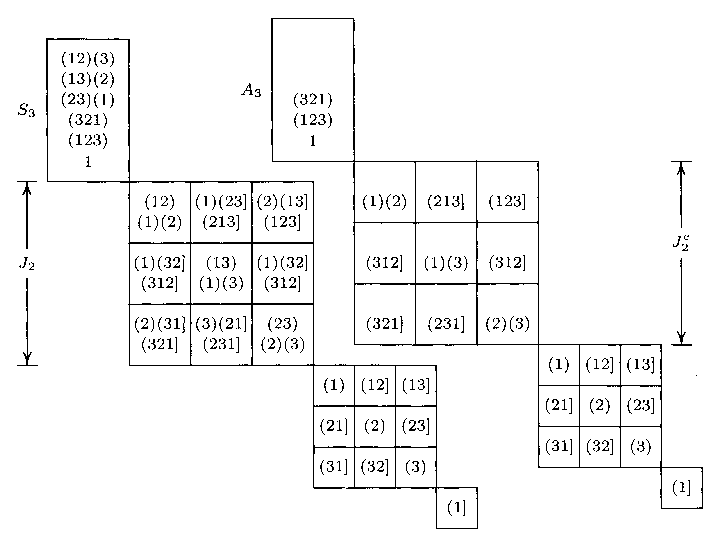
\includegraphics{chap06-vend-scan-01.eps}
\end{figure}

\begin{equation*}
K=\bigcup_{m=-\infty}^{\infty}P^{m}\mathscr{T}_{x},
\end{equation*}
$\mathscr{T}_{x}$ being a parabolic sector at $x$. Now define (cf. Figure):
\begin{equation*}
\mathscr{S}_{x}=\{x\}\bigcup K,\qquad x\in\mathscr{P}.
\end{equation*}
Let $\mathbf{B}$ be the family of all $\mathscr{S}_{x}$ for $x\in \mathscr{D}^{+}$. It is immediate that $\mathbf{B}$ has the finite intersection property and that each point of $\mathscr{D}^{+}$ lies in a member of $\mathbf{B}$. Hence $\mathbf{B}$ is the basis of a topology $\mathbf{X}$ for $\mathscr{D}^{+}$.

Note that if $x$ is not a parabolic vertex, there are relatively compact sets $\mathscr{S}_{x}$. But this is no longer true when $x$ is a parabolic vertex. Indeed, a sequence tending in the conventional sense to $x$ along the boundary of a horocycle does not converge in the topology $\mathbf{X}$.

We observe that $\mathscr{D}^{+}$ is a connected space. In fact, $\mathscr{D}$ is a connected subset of $\mathscr{D}^{+}$ because\index{Poincar\'{e}} the relative topology of $\mathscr{D}$ as a subset of $\mathscr{D}^{+}$ is the same as its relative topology considered as a subset of the sphere, and we have assumed $\mathscr{D}$ is a region in the latter topology. The points of $\mathscr{P}$ are boundary points of $\mathscr{D}$ relative to $\mathscr{D}^{+}$. Hence $\mathscr{D}^{+}$ is a connected set (and therefore a connected space), for the addition of boundary points leaves a set connected (\ref{ch02:chap02}. \ref{ch02:sec2I}. Th. \ref{ch02:thm2}).

Finally, $VA$ is open if $A$ is open and $V\in \Gamma$, i.e., the topology of $\mathscr{D}^{+}$ is preserved by the group action. We need prove this only for the sets in the basis. But $V\mathscr{S}_{x}$ is a set of the form $\mathscr{S}_{Vx}$.


\subsection{}\label{ch06:sec3B} We now construct the \emph{orbit space} (quotient space)\index{quotient space} of $\mathscr{D}^{+}$ modulo $\Gamma$. Denote by $[x]$ the orbit $\Gamma x =\{V_{x}|V\in\Gamma\}$. We define $S=\Gamma\backslash \mathscr{D}^{+}$ to be the set of orbits $[x]$ for $x\in \mathscr{D}^{+}$. (A model of $S$ is the closure of a connected fundamental region in which certain identifications have been made among the boundary points.)

For the purpose of constructing a topology on $S$ we define a \emph{projection mapping}\index{projection mapping} $\sigma$ from $\mathscr{D}^{+}$ onto $S:\sigma$ is the function that sends each $x$ of $\mathscr{D}^{+}$ into its orbit $[x]$. We have $\sigma(x)=\sigma(\Gamma x)=[x]$, and
\begin{equation*}
\sigma(\mathscr{D}^{+})=S.
\end{equation*}
Also,
\begin{equation*}
\sigma^{-1}\{\sigma(A)\}=\Gamma A,\qquad A\subset \mathscr{D}^{+}.
\end{equation*}

Now $S$ becomes a topological\index{quotient space!topology for} space if we define $A \subset S$ to be open if and only if its inverse image $\sigma^{-1}(A)$ is open in $\mathscr{D}^{+}$. This topology, which is induced by $\sigma$, we call $\mathbf{X}^{\prime}$. Moreover $\sigma$ is then a continuous mapping of $\mathscr{D}^{+}$ onto $S$ (cf.~\ref{ch02:chap02}.~\ref{ch02:sec3G}). In addition $S$ is connected, for it is the continuous image of the connected set $\mathscr{D}^{+}$ (cf.~\ref{ch02:chap02}.~\ref{ch02:sec3H}).

We now show that $\sigma$ is an open mapping. Let $O \subset\mathscr{D}^{+}$ be open; we have to show that $\sigma(O)$ is open. Now $\sigma^{-1}|\sigma(O)]=\Gamma(O)$; since the right member is open, so is the left, and this shows, by the definition, that $\sigma(O)$ is open.


\subsection{}\label{ch06:sec3C} The next step is to prove that $S$ is a Hausdorff space\index{quotient space!as Hausdorff space}. Let $[x]$ and $[y]$ be distinct points of $S$; then $x\not\in\Gamma y$ and $y \not\in\Gamma x$. As a first case assume $x,\,y$ are both in $\mathscr{D}$.

Choose a neighborhood $\overline{\mathscr{S}}_{x}$ which is compact in $\mathscr{D}$. Any compact neighborhood of $x$ contains only a finite number of points of $\Gamma y$ (cf.~\ref{ch04:chap04}.~\ref{ch04:sec1H}).\footnote{Since the relative topology of $\mathscr{D}$ coincides with the usual topology of the sphere, we are permitted to use the results of Ch.~\ref{ch04:chap04}.} Hence there is a compact neighborhood $X$ of $x$ which does not meet $\Gamma y$ at all. Having chosen $X$ we now note, by the same reasoning, that only a finite number of $VX,\,V\in \Gamma$, meet any given compact neighborhood of $y$, so it is possible to choose a compact neighborhood $Y$ of $y$ which does not meet $\Gamma X$. Thus $\Gamma X\cap\Gamma Y =0$, for if $V X$ meets $WY\ (V,\, W\in\Gamma)$, then $Y$ meets $W^{-1}VX$. It follows that $\sigma(X)$ is disjoint from $\sigma(Y)$. But $\sigma(X)$ is a neighborhood of $[x]$. For $X$ contains an open neighborhood $O$ of $x$; hence $[x]\in \sigma(O) \subset\sigma(X)$, and $\sigma(O)$ is open since $\sigma$ is an open mapping. Similarly $\sigma(Y)$ is a neighborhood of $[y]$. This shows that $[x]$ and $[y]$ have disjoint neighborhoods.

Next we let $x,\,y\in \mathscr{P}$; we may assume both points are in the same fundamental region $R_{0}$. Let $x=x_{1}$ be in the cycle $(x_{1},\,\cdots\,, x_{s})$ and $y=y_{1}$ in the cycle $(y_{1},\, \cdots,\, y_{t})$. A set $\mathscr{S}_{x}$ cuts out an open curvilinear triangle $\Delta_{1}$ lying in $R_{0}$ and having a vertex $x;\,\Delta_{1}$ has triangular images $\Delta_{2},\,\cdots,\,\Delta_{\delta}$ at $x_{2},\,\cdots,\,x_{\delta}$, respectively. Similarly $\mathscr{S}_{y}$ cuts out a triangle $\Delta^{\prime}_{1}$ at $y_{1}$ with images $\Delta_{2}^{\prime},\,\ldots,\,\Delta^{\prime}_{t}$ at $y_{2},\cdots,y_{t}$. $\mathscr{S}_{x}$ consists entirely of images of $\{\Delta_{i}\};\mathscr{S}_{y}$, entirely of images of $\{\Delta_{j}^{\prime}\}$. We shall select $\mathscr{S}_{x},\,\mathscr{S}_{y}$ so small that the sets $\{\Delta_{i}\},\, \{\Delta_{j}^{\prime}\}$ are mutually disjoint.

We assert $\Gamma \mathscr{S}_{y}$ does not meet $\mathscr{S}_{x}$. If this is not the case, $V\Delta_{k}$ meets $W\Delta_{l}^{\prime}$ for some $V,\,W$ in $\Gamma$ and some $k,\,l$. Since $V\Delta_{k}$ lies entirely in one fundamental region and likewise $W\Delta_{l}^{\prime}$, they must lie in the \emph{same} fundamental region. Hence $V=W$ and $\Delta_{k}$ intersects $\Delta_{l}^{\prime}$, a contradiction.

The same argument can be modified slightly to cover the last case: $x\in \mathscr{P},\,y\in \mathscr{D}$.

This concludes the proof that $(S,\, \mathbf{X}^{\prime})$ is a Hausdorff space.


\subsection{}\label{ch06:sec3D} We are ready to introduce an analytic structure on\index{quotient space!analytic structure on} $S$: for each $[x]\in S$ we must exhibit an open neighborhood $U_{x}$ of $[x]$ and a homeomorphism $\Phi_{x}$ mapping $U_{x}$ onto an open set $D$ of the euclidean plane. For $U_{x}$ we take simply
\begin{equation*}
U_{x}=\sigma(\mathscr{S}_{x}^{\ast}),
\end{equation*}
where $\mathscr{S}_{x}^{\ast}$ is a specially selected set of the basis for the topology of $\mathscr{D}^{+}$. As we noted in~\ref{ch06:sec3C}, $U_{x}$ is an open neighborhood of $[x]$. At the moment we shall demand only that $\mathscr{S}_{x}^{\ast}-x$ contain no fixed points of $\Gamma$. Later we shall impose other conditions.

It is convenient to define the mappings
\begin{equation*}
\tag{$^{\ast}$} \sigma_{x}= \mathrm{restriction\ of}\ \sigma\ \mathrm{to}\ \mathscr{S}_{x}^{\ast},\qquad \Phi_{x}=\tau_{x}\circ\sigma_{x}^{-1};
\end{equation*}
$\Phi_{x}$ will be the desired homeomorphism. Here $\tau_{x}=\tau_{x}(z)$ is a function from $\mathscr{S}_{x}$ to the euclidean plane, the form of which depends on whether $x$ is a nonfixed point, elliptic vertex, or parabolic vertex; it will be defined presently. Certain assertions, however, can be made regardless of the nature of $x$. For example, $\sigma_{x}$ is continuous, because it is the restriction of a continuous function. We prove it is open. Let $A$ be open in $\mathscr{S}_{x}^{\ast}$; it is absolutely open because $\mathscr{S}_{x}^{\ast}$ is open. Then $\sigma_{x}A=\sigma A$ is open in $S$ because $\sigma$ is an open mapping. But $\sigma_{x}A\subset U_{x}$, so $\sigma_{x}A=\sigma_{x}A\cap U_{x}$ is open in $U_{x}$. Hence, for all $x\in \mathscr{D}^{+},\,\sigma_{x}$ is an open, continuous mapping. \emph{In order to show} $\Phi_{x}$ \emph{is a homeomorphism it is sufficient to prove that it is} 1-1 \emph{and that} $\tau_{x}$ \emph{is open and continuous}.

First, let $x$ be a point that is not fixed by any element of $\Gamma$. Choose for $\mathscr{S}_{x}$ a relatively compact disk $\mathscr{S}_{x}^{\ast}$ containing no equivalent points. Define
{\def\theequation{9a}
\begin{equation}
\label{ch06:eqn9a} \tau_{x}(z)=z -x.
\end{equation}}
It is evident that $\Phi_{x}$ maps $U_{x}$ onto a disk $D$ in a 1-1 manner. Obviously $\tau_{x}$ is open and continuous. Hence $\Phi_{x}$ is a homeomorphism.

Next, let $x$ be an elliptic fixed point of order $l$ and $x^{\prime}$ the fixed point conjugate to $x$. Let $E$ generate the subgroup $\Gamma_{x}$. We select for $\mathscr{S}_{x}$ a relatively compact disk $\mathscr{S}_{x}^{\ast}$ whose boundary is a fixed circle of $E$. We demand also that it meet none of its images except those under powers of $E$. Define
{\def\theequation{9b}\begin{equation}
\label{ch06:eqn9b} \tau_{x}(z)=((z-x)/(z-x^{\prime}))^{l}.
\end{equation}}
Observe that $\tau_{x}$ maps $\mathscr{S}_{x}^{\ast}$ in an $l$ to 1 manner on an open disk $D$ and $\tau_{x}^{-1}$ carries a point $w\in D$ into $l$ points $\{z_{i}\}$ in $\mathscr{S}_{x}^{\ast}$ that are equivalent under powers of $E$ (cf.~\ref{ch02:chap02}. \ref{ch02:sec8E}). But $\sigma_{x}$ maps the set $\{z_{i}\}$ onto a single point of $S$. It is clear, then, that $\Phi_{x}$ is 1-1 from $U_{x}$ to $D$. Since $\tau_{x}$ is regular in $\mathscr{S}_{x}^{\ast}$, it is open and continuous there. Again $\Phi_{x}$ is a homeomorphism.

The final case for consideration is $x\in \mathscr{P}$. We require that $\mathscr{S}_{x}^{\ast}$ intersect none of its images except those under powers of $P$, the generator of $\Gamma_{x}^{\ast}$. From~\ref{ch02:chap02}. \ref{ch02:sec8E} we take certain facts regarding the function
{\def\theequation{9c}\begin{equation}
\label{ch06:eqn9c} \tau_{x}(z)=e(1/c(z-x)),
\end{equation}}
where
\begin{equation*}
z^{\prime}=Pz,\qquad \frac{1}{z^{\prime}-x}=\frac{1}{z-x}+c.
\end{equation*}
$\tau_{x}$ maps $\mathscr{S}_{x}^{\ast}$ onto an open disk $D$ about the origin, the point $x$ going into $0$. The mapping is infinitely many to one; the inverse image of $\tau_{x}(z)=w\neq 0$ is $\{P^{m}z,\,m= \mathrm{integer}\}$, whereas $0$ corresponds only to $x$. Moreover, $\tau_{x}$ is still continuous at $x$.

It follows that for $[y]\in U_{x},\,\sigma_{x}^{-1}([y])=\{P^{m}y\}$ and $\tau_{x}\circ\sigma_{x}^{-1}([y])=\tau_{x}(y)$. Distinct points $[y_{1}]$ and $[y_{2}]$ in $U_{x}$ have inequivalent images in $\mathscr{S}_{x}^{\ast}$ and therefore map into distinct points of $D$. Hence $\Phi_{x}$ is 1-1.

We know that $\tau_{x}$ is continuous on all of $\mathscr{S}_{x}^{\ast}$. We have to show it is open, and it is sufficient to prove that it carries sets of the basis into open sets. That $\tau_{x}$ maps open disks not passing through $x$ into open disks of $D$ is obvious, for it is regular except at $x$. A disk through $x$ is mapped by $\tau_{x}$ onto a disk surrounding the origin. It follows that $\tau_{x}$ is an open mapping.

We have shown in each case that $\Phi_{x}$ is a homeomorphism of $U_{x}$ onto an open disk $D$ of the complex plane.


\subsection{}\label{ch06:sec3E} The final step is to show that the neighbor relations $\Phi_{x}\circ\Phi_{y}^{-1}$, when defined, are directly conformal functions on their domains.

Suppose $\Phi_{x},\,\Phi_{y}$ are homeomorphisms of neighborhoods $U_{x}=\sigma(\mathscr{S}_{x}^{\ast})$,
$ U_{y}=\sigma(\mathscr{S}_{y}^{\ast})$, respectively, and let $U_{x}\cap
U_{y}=D^{\prime}\neq 0$. Select $x,\,y\in \mathscr{D}^{+}$ so that $\mathscr{S}_{x}^{\ast}$ intersects $\mathscr{S}_{y}^{\ast}$ in $D\neq 0$. The equation
\begin{equation*}
\Phi_{x}\circ\Phi_{y}^{-1}=\tau_{x}\circ \sigma_{x}^{-1}\circ\sigma_{y}\circ \tau_{y}^{-1}=\tau_{x}\circ \tau_{y}^{-1},
\end{equation*}
with domain $\Phi_{y}(D^{\prime})=\tau_{y}(D)$, can be verified by a consideration of cases depending on the character of $x$ and $y$.

Reference to the definitions (\ref{ch06:eqn9a})--(\ref{ch06:eqn9c}) shows that $\tau_{x}(z)$ is conformal except possibly at $z=x;\tau_{x}^{-1}(w)$ is conformal except possibly at $w=0$. From our choice of $\mathscr{S}_{x}^{\ast},\,\mathscr{S}_{y}^{\ast}$ (cf.~\ref{ch06:sec3D}) we are able to conclude that $D$ contains no fixed points. The set $\tau_{y}(D)$, therefore, does not contain the origin and so $\tau_{y}^{-1}$ is conformal on this set. The domain of $\tau_{x}$ is $D$ and $\tau_{x}$ is conformal there. This shows that $\Phi_{x}\circ\Phi_{y}^{-1}$ is a directly conformal mapping, as asserted.

We have now finished the proof of the following result:


\begin{theorem*}
Let $\Gamma$ be a discontinuous function group on a domain of existence $\mathscr{D}$. Then $S=\Gamma\backslash \mathscr{D}^{+}$, together with the analytic structure induced on it by the projection map $\sigma$, is a Riemann surface\index{quotient space!as Riemann surface}.
\end{theorem*}

\subsection{}\label{ch06:sec3F} A very important class of Riemann surfaces are the \emph{compact}\index{Riemann surface!compact} surfaces. We would like to prove that $S$ is compact if and only if the fundamental region\index{compact Riemann surface!and fundamental region}\index{Riemann surface!compact, and fundamental region} $R_{0}$ of $\Gamma$ is compact in $\mathscr{D}^{+}$. We shall be almost successful in our aim.

\emph{Warning}. The theorems of this subsection will appear strange to the reader familiar with the literature. There it is emphasized that, for example, the Riemann surface $\Gamma\backslash \mathscr{H}$, where $\Gamma$ is the modular group and $\mathscr{H}$ is the upper half-plane, is not compact, since the fundamental region of $\Gamma$ is not relatively compact in $\mathscr{H}$. But we have considered $\Gamma\backslash \mathscr{H}^{+}$ rather than $\Gamma\backslash \mathscr{H}$, and $\Gamma\backslash \mathscr{H}^{+}$ is compact, as we shall show. Moreover, we have always assumed $\mathscr{D}$ is a domain of existence, i.e., a \emph{maximal} region preserved by $\Gamma$. Consider the hyperbolic cyclic group $\Gamma$ generated by a transformation $T$ that preserves the unit disk $\mathscr{U}$. Certainly $\Gamma\backslash \mathscr{U}$ is not compact; it is, in fact, homeomorphic to a sphere from which two disjoint closed disks have been removed. But the domain of existence of $\Gamma$ is $\mathscr{D}=\mathscr{D}^{+}=\mathscr{L}-\{z_{1},\,z_{2}\}$, where $\{z_{i}\}$ are the fixed points of $T$, and $\Gamma\backslash {\mathscr{D}^{+}}$ is a compact surface, namely, a torus. These examples show that it is essential to observe particularly the base space which is being reduced by the group.

Let us remark that a finite number of parabolic vertices in $R_{0}$ does not of itself make $R_{0}$ noncompact. Consider the closed triangular region $\overline{\Delta}_{x}$ formed by intersecting the closure of a horocycle at $x$ with $\overline{R}_{0}$. $\overline{\Delta}_{x}$ \emph{is compact in the topology we have assigned to $\mathscr{D}^{+}$}. For any open set covering $x$ must contain a horocycle passing through $x$, and when this is subtracted from $\Delta_{x}$ the remainder is compact in $\mathscr{D}$.

Suppose now $\bar{R}_{0}$ is compact in $\mathscr{D}^{+}$. We have
\begin{equation*}
S=\sigma(\mathscr{D}^{+})=\sigma(\bar{R}_{0}),
\end{equation*}
for each $z$ in $\mathscr{D}^{+}$ has at least one equivalent point in $\bar{R}_{0}$. Since $\sigma$ is continuous, $S$ is compact.

Conversely, suppose $S$ is compact. We show first that $R_{0}$ has a finite number of sides. Otherwise we can choose an infinite set of points $\{z_{i}\}$, each $z_{i}$ being an inner point of a different side of $R_{0}$. Since $z_{i}$ is equivalent to exactly one other boundary point of $R_{0}$, we can select the $\{z_{i}\}$ to be mutually inequivalent. Setting $q_{n}=\sigma(z_{n})$ we can assert that $\{q_{n}\}$ is composed of distinct points and, because of the compactness of $S$, possesses an accumulation point $q\in S$. Certainly $q$ has inverse images lying in $\mathscr{D}^{+}$. Let $\zeta$ be one of these images lying in $\bar{R}_{0}$. Since every neighborhood $N$ of $\zeta$ maps into a neighborhood of $q$, we can say that $N$ contains a $\Gamma$-image of infinitely many $z_{i}$. Obviously $\zeta$ is not an inner point of $R_{0}$. Nor is it an inner point of a side of $R_{0}$ or an ordinary vertex, for we can choose $N$ so that it contains the equivalent of at most one $z_{i}$. Suppose $\zeta$ is a parabolic vertex. The reasoning of~\ref{ch05:chap05}. \ref{ch05:sec3A} can be used to show there is an $N$ not containing the image of any $z_{i}$. It follows that $\zeta$ is a boundary point of $\mathscr{D}$ but not a parabolic vertex. That is, $\zeta \not\in \mathscr{D}^{+}$, a contradiction. Therefore $R_{0}$ has a finite number of sides.

By almost the same argument one can prove that $\Gamma$ has a finite number of elliptic and parabolic fixed point classes. We have to know, however, that no set of fixed points of $\Gamma$ can accumulate in $\mathscr{D}$. This is obvious when the fixed points are parabolic; for elliptic fixed points, the fact has been proved in III. Ex.3-2. Cf. Note 13, p. 401.

In order to prove that $\bar{R}_{0}$ is compact in $\mathscr{D}^{+}$, we seem to be forced to make the following assumption, as we did in~\ref{ch05:chap05}. 4:

\def\theassumption{\Alph{assumption}}
\begin{assumption}\label{ch06:assA} If the fundamental region $R_{0}$ of a function group $\Gamma$ has a finite number of sides, $\bar{R}_{0}$ meets $\mathrm{Bd}\,\mathscr{D}$ only in parabolic vertices.
\end{assumption}

This assumption is satisfied by all principal-circle groups\footnote{Recall that $\bar{R}_{0}$ may meet the principal circle in \emph{ordinary} points, which are not, therefore, parabolic, but if it meets the principal circle in a \emph{limit} point, this point must be a parabolic vertex. provided $R_{0}$ is finitely-sided.} (\ref{ch04:chap04}. Th. \ref{ch04:sec6G}). The converse of the assumption is a known theorem (\ref{ch04:chap04}.~\ref{ch04:sec4J}).

Let $x_{i},\,i=1,\,\cdots,\,s$, be the parabolic vertices in $R_{0}$ and let $\overline{\Delta}_{i}$ be the intersection of $\overline{R}_{0}$ with the closure of a horocycle through $x_{i}$. Since $\overline{\Delta_{i}}$ is compact, $\bigcup\nolimits_{i=1}^{s}\overline{\Delta}_{i}$ is compact. Let $G=R_{0}- \bigcup_{i=1}^{s}\overline{\Delta}_{i}$. Because of Assumption A all boundary points of $G$ lie in $\mathscr{D}$, and a simple argument demonstrates the compactness of $\overline{G}$. Hence $\bar{R}_{0}$ is compact.

We have proved:

\begin{theorem*}
Let $\Gamma$ be a function group. If $\bar{R}_{0}$ is compact in $\mathscr{D}^{+}$, then $S=\Gamma\backslash \mathscr{D}^{+}$ is a compact Riemann surface. If $S$ is compact, $R_{0}$ has a finite number of sides and $\Gamma$ has a finite number of classes of elliptic fixed points. Moreover, $\bar{R}_{0}$ is compact in $\mathscr{D}^{+}$ if Assumption \emph{A} is satisfied.
\end{theorem*}

\subsection{}\label{ch06:sec3G} The theorem we\index{Riemann surface!compactification of} have just proved is not the usual one. It is customary to consider $\Gamma\backslash \mathscr{D}$, not $\Gamma\backslash
\mathscr{D}$. Denote $\Gamma\backslash \mathscr{D}$ by $S^{\prime}$. Since $\mathscr{D}$ is open, we can use the relative topology of the sphere. Call $\Phi^{\prime}$ the subfamily of $\Phi$ consisting of those homeomorphisms whose domains are entirely contained in $S^{\prime}$. The reader will have no difficulty in verifying that $S^{\prime}$ is a Riemann surface.

The result usually proved is as follows:


\begin{theorem*}
The Riemann surface $S^{\prime}$ is compact if and only if the fundamental region $R_{0}$ is relatively compact in $\mathscr{D}$.
\end{theorem*}

The point of the proof we are about to give is that it avoids Assumption~\ref{ch06:assA}.

Suppose $S^{\prime}$ is compact. Cover each point $x$ of $\bar{R}_{0}\cap \mathscr{D}$ by a relatively compact disk $N(x)$ lying in $\mathscr{D}$. Let $U(x)=\sigma(N(x))$. Since $\sigma$ is an open mapping, $U(x)$ is open and the sets $\{U(x) |x \in\bar{R}_{0}\cap \mathscr{D}\}$ form an open covering of $S^{\prime}$. There is a finite subset $\{U(x_{1}),\cdots,U(x_{s})\}$ that covers $S^{\prime}$. Hence $\{N(x_{1}),\, \cdots,\, N(x_{s})\}$ covers $R_{0}$. Since $\bar{N}(x_{1}) \cup\cdots \cup\bar{N}(x_{s})$ is compact in $\mathscr{D}$, it follows that $R_{0}$ is relatively compact in $\mathscr{D}$. The proof of the converse is the same as in Theorem 3F.

The procedure we employed in the construction of $S$ (cf. \ref{ch06:sec3A}--\ref{ch06:sec3E}) is equivalent to ``compactifying'' $S^{\prime}$ by the adjunction of neighborhoods of the images of the parabolic vertices.

\subsection{}\label{ch06:sec3H} The fundamental region\index{orbit} of $\Gamma$ can be used to calculate the genus of $S$.


\begin{theorem*}
Let $S=\Gamma\backslash \mathscr{D}^{+}$ be compact\index{Riemann surface!compact}. Let $\bar{R}_{0}^{\prime}$ be $\bar{R}_{0}$ with equivalent points on the boundary identified. Then $\bar{R}_{0}^{\prime}$ and $S$ are homeomorphic. If $R_{0}$ is connected,
\begin{equation}
\label{ch06:eqn10} g=\frac{1}{2}(n+1-c),
\end{equation}
where $g$ is the genus of $S,\,c$ is the number of cycles and $n$ the number of sides of $\bar{R}_{0}^{\prime}$. ($A$ pair of conjugate sides in $R_{0}$ is counted as one side in $\bar{R}_{0}^{\prime}$.)
\end{theorem*}

Define $\sigma_{1}$ as the restriction of $\sigma$ to $\bar{R}_{0}^{\prime}$. Clearly $\sigma_{1}$ maps $\bar{R}_{0}^{\prime}$ on $S$ in a 1-1 manner, since equivalent points on Bd $\bar{R}_{0}$ are identified in $\bar{R}_{0}^{\prime}$. In order that $\sigma1$ be a homeomorphism it is necessary to assign to $\bar{R}_{0}^{\prime}$ a topology that is consistent with the group $\Gamma$. Define a neighborhood $\mathscr{N}_{x}^{\prime}$ of $x\in\bar{R}_{0}^{\prime}$ as follows:
\begin{equation*}
\mathscr{N}_{x}^{\prime}=\Gamma\mathscr{N}_{x}\cap\bar{R}_{0}^{\prime},
\end{equation*}
where $\mathscr{N}_{x}$ is a neighborhood of $x$ in the topology of $\mathscr{D}^{+}$. It is easily checked that this is a valid topology. We retain on $S$ the topology $\mathbf{X}^{\prime}$ defined in 3B, i.e., $\mathbf{X}^{\prime}$ is the topology induced by $\sigma$ on $\mathscr{D}^{+}$. Note that the topology induced by $\sigma_{1}$ on $\bar{R}_{0}^{\prime}$ coincides with $\mathbf{X}^{\prime}$.

It is now an easy matter to check that $\sigma_{1}$ is a topological mapping of $\bar{R}_{0}^{\prime}$ on $S$. The neighborhoods of the various classes of points of $\bar{R}_{0}^{\prime}$ are shown in the Figures; sides connected by arrows must be identified.

We take advantage of the homeomorphism to calculate the genus of $S$ by applying Euler's polyhedron formula to $\bar{R}_{0}^{\prime}$. The number of inequivalent vertices, i.e., the number of cycles, $c$, must be used for the number of vertices in the formula, and the number of edges is $n$, since there are $n$ pairs of conjugate sides. We have assumed $R_{0}$ is connected, so there is one cell. The formula \eqref{ch06:eqn10} follows.

\begin{figure}[!h]
\includegraphics{chap06-vend-scan-02.eps}
\end{figure}

\subsection{}\label{ch06:sec3I} The domain $\mathscr{D}$ serves in a natural way as a covering surface\index{domain of existence!as covering surface} of $S^{\prime}=\Gamma\backslash \mathscr{D}$. With the neighborhood structure $\mathbf{X}$ defined in 3A and the homeomorphisms $\{\tau_{x}\}$ of (9), $\mathscr{D}$ becomes a manifold. The projection mapping from $\mathscr{D}$ into $S$ is simply $\sigma$. That is, the points lying above a given $q\in S^{\prime}$ are the points $\Gamma x$, where $\sigma x =q$. (Cf. \ref{ch06:sec1G}, \ref{ch06:sec1J}.)

We know $\sigma$ is continuous and open. A nonfixed point $x$ has a neighborhood $\mathscr{S}_{x}$ that meets none of its $\Gamma$-images. Thus $\sigma$ is a homeomorphism of $\mathscr{S}_{x}$ onto its image. Now let $y$ be a fixed point. No fixed point is contained in $\mathscr{S}_{y}-y$ if we choose $\mathscr{S}_{y}$ small enough. Hence each point of $\mathscr{S}_{y}-y$ has a neighborhood that is mapped topologically by $\sigma$. It follows that $(\mathscr{D},\,\sigma)$ is a branched covering of $S^{\prime}$.

The branch points are, of course, the elliptic fixed points. A point fixed by a generating elliptic transformation of period $l$ is a branch point of order $l-1$.

Let $\gamma$ be a curve in $S^{\prime}$ with initial point $\gamma_{0}$ and let $x_{0}\in \mathscr{D}$ be a point lying above $\gamma_{0}$. Now $x_{0}$ lies in the closure of some fundamental region, say $\bar{R}_{0}$. As before, denote by $\sigma 1$ the restriction of $\sigma$ to $\bar{R}_{0}^{\prime}$ and assign to $\bar{R}_{0}^{\prime}$ the topology described in 3H. Then $\sigma 1$ is a homeomorphism. Hence $\sigma_{1}^{-1}(\gamma)$ is a curve in $\mathscr{D}$, its initial point is $x_{0}$, and
\begin{equation*}
\sigma[\sigma_{1}^{-1}(\gamma)]=\sigma_{1}\circ\sigma_{1}^{-1}(\gamma)=\gamma.
\end{equation*}
It follows that $(\mathscr{D},\,\sigma)$ is unlimited.


\begin{theorem*}
$(\mathscr{D},\,\sigma)$ is a \emph{(}branched\emph{)} unlimited covering surface of $S^{\prime}=\Gamma\backslash \mathscr{D}$. Denote by $\mathscr{F}$ the set of fixed points of $\Gamma$; then $(\mathscr{D}-\mathscr{F},\, \sigma)$ is a smooth unlimited covering of $S^{\prime}-\sigma(\mathscr{F})$. The mapping $\sigma$ is analytic\index{projection mapping!is analytic} on the domain $\mathscr{D}-\mathscr{F}$.
\end{theorem*}

The first statement has been proved. The second is an immediate corollary. The last assertion follows from 1K.

\textit{Remark.} If there are no fixed points of $\Gamma$ in $\mathscr{D}$ and if $\mathscr{D}$ is simply connected, $(\mathscr{D},\,\sigma)$ is smooth, unlimited, and simply connected, and is therefore the universal covering surface of $S^{\prime}$.

\subsection{}\label{ch06:sec3J} We remark finally that the group of covering transformations\index{group of covering transformations} of the covering surface $(\mathscr{D},\, \sigma)$ is precisely $\Gamma$. Obviously $\sigma \circ V=\sigma$ for each $V\in\Gamma$. Hence $V$ is a covering transformation. On the other hand suppose $h$ is a covering transformation, i.e., $h$ is a homeomorphism of $\mathscr{D}$ which satisfies $\sigma \circ h=\sigma$. Let $z_{0}$ be a nonfixed point of $\mathscr{D}$. There is a neighborhood $N$ of $z_{0}$ that is mapped topologically by $\sigma$. Then $h(N)$ is a neighborhood of $h(z_{0})$ that also is mapped topologically by $\sigma$. Denoting by $\sigma_{1},\,\sigma_{2}$ the restrictions of $\sigma$ to $N$ and $h(N)$, respectively, we can assert $h=\sigma_{2}^{-1}\circ \sigma_{1}$ in $N$. Thus $h$ is analytic since $\sigma_{1}$ and $\sigma_{2}$ are (1K).

Now $\sigma \circ h=\sigma$ implies $hz_{0}\in\Gamma z_{0}$, or $hz_{0}=Vz_{0}$ for some $V\in\Gamma$. Moreover $\sigma_{2}\circ h=\sigma_{2} \circ V$ in $N$ since both are equal to $\sigma_{1}$. Multiplying by $\sigma_{2}^{-1}$, we obtain $h=V$, valid in $N$. But $\mathscr{D} -\mathscr{F}$ is still connected, where $\mathscr{F}$ is the set of fixed points. We can continue the relation $h=V$ to any point of $\mathscr{D}-\mathscr{F}$ along a curve not passing through a point of $\mathscr{F}$, and by the principle of analytic continuation we conclude that $h=V$ throughout $\mathscr{D}$. Hence:


\begin{theorem*}
$\Gamma$ is the group of covering transformations of $(\mathscr{D},\,\sigma)$.
\end{theorem*}

\emph{Remark}. It is impossible to extend $(\mathscr{D},\,\sigma)$ to a covering surface of $S$. The space $\mathscr{D}^{+}$ is not a manifold, for the neighborhoods of the parabolic vertices (points of $\mathscr{D}^{+}-\mathscr{D}$) are not locally compact.

\subsection{}\label{ch06:sec3K} We turn now to the converse problem: given $S$, find $\Gamma$ and $\mathscr{D}$ so that $\Gamma\backslash \mathscr{D}=S$. Here we shall assume that $\mathscr{D}=\mathscr{U}$, the open unit disk, in which case the problem always has a solution. (Note that the space is $\mathscr{D}$ rather that $\mathscr{D}^{+}$.)

Let $\hat{S}=(\hat{S},\,\pi)$ be the universal covering surface of $S$ (cf.~\ref{ch06:sec1H}); $\pi$ is a continuous mapping of $\hat{S}$ into $S$ (projection mapping).
$\hat{S}$ is simply connected. The mapping theorem of Riemann states there is a function $f$ that maps $\hat{S}$ conformally and one-to-one on a normal region of the complex sphere (sphere, complex plane, or unit disk). (Cf. \citeauthor{Ahlfors0000a}\index{Ahlfors-Sario} [\ref{Ahlfors}, Ch. \ref{ch03:chap03}, Th. 11 G, p. 181].) The first two regions are in the nature of exceptions and will be disregarded here. We assume then that $\hat{S}$ is conformally equivalent to $\mathscr{U}$ (\emph{hyperbolic case}): $f(\hat{S})=\mathscr{U}$.

Let $H$ be the group of covering transformations of $\hat{S}$. Each $h\in H$ is a conformal self-mapping of $\hat{S}$ (cf. \ref{ch06:sec1K}). Hence $V=f\circ h \circ f^{-1}$ is a conformal homeomorphism of $\mathscr{U}$ and therefore a linear transformation (\ref{ch02:chap02}.~\ref{ch02:sec8D}). The group $H$ corresponds to a group $\Gamma$ of linear transformations of $\mathscr{U}$ on itself: $\Gamma=f\circ H\circ f^{-1}$. Points in $\mathscr{U}$ which are equivalent under $\Gamma$ correspond to points in $\hat{S}$ which have the same projection (under $\pi$) in $S$.

1) \emph{No element of} $\Gamma$ \emph{except the identity has a fixed point in} $\mathscr{U}$. This means $\Gamma$ has no elliptic substitutions. To prove the result, note that a fixed point of $V\in \Gamma$ corresponds to a fixed point of $h=f^{-1}\circ V\circ f\in H$, which is possible only if $h$ is the identity (1I).

2) $\Gamma$ \emph{is discontinuous in} $\mathscr{U}$. Suppose on the contrary that $z,\,z_{0}$ are points of $\mathscr{U}$ and $\{V_{n}\}$ is a set of distinct elements of $\Gamma$ such that $V_{n}z\rightarrow z_{0}$. The $\{V_{n}z\}$ are all distinct, since the transformations of $\Gamma$ are free of fixed points. Write
\begin{equation*}
h_{n}=f^{-1}\circ V_{n}\circ f\in H,\qquad f^{-1}(z)=\hat{q},\qquad f^{-1} (V_{n}z)=\hat{q}_{n},\qquad f^{-1}(z_{0})=\hat{q}_{0}.
\end{equation*}
There is a neighborhood $\hat{N}$ of $\hat{q}_{0}$ which covers a neighborhood $N$ of $q_{0}=\pi(\hat{q}_{0})$ exactly once. On the other hand, $f(\hat{N})$ is a neighborhood of $z_{0}$ and contains infinitely many $V_{n}z$; hence $\hat{N}$ contains infinitely many $\hat{q}_{n}$. The $\hat{q}_{n}$ are distinct, since the $V_{n}z$ are. Since $V_{n}z$ is equivalent to $V_{m}z$, it follows that $\hat{q}_{n}$ and $\hat{q}_{m}$ project into the same point of $\pi(N)$, which means $\pi$ is not 1-1 between $\hat{N}$ and $\pi(\hat{N})$, a contradiction.

3) \emph{The Riemann surface} $\Gamma\backslash \mathscr{U}=S_{1}$ \emph{is conformally equivalent to} $S$. \emph{An equivalent statement}: \emph{the diagram on p. 209 is commutative}.

\noindent Consider the mapping $g:S\rightarrow S_{1}$ given by $p_{1}=g(p)=\sigma_{1} \circ f\circ\pi^{-1}(p)$, where $\sigma_{1}$ is the projection map $\mathscr{U}  \rightarrow\Gamma\backslash \mathscr{U}$. $g$ is single-valued even though $\pi^{-1}$ is not, for $\sigma_{1}$ identifies the points of the set $f\circ\pi^{-1}(p)$, which are $\Gamma$-equivalent. Next, $g$ is onto. Indeed, let $p_{1}\in S_{1}$ and $\sigma_{1}(z)=p_{1}$; then $\pi \circ f^{-1}(z)\in S$. From $g\circ \pi=\sigma_{1}\circ f$ we deduce
\begin{equation*}
g(\pi\circ f^{-1}(z))=g\circ\pi(f^{-1}(z))=\sigma_{1}\circ f(f^{-1}(z))=\sigma_{1}(z)=p_{1}.
\end{equation*}
Finally, $g$ is 1-1 from $S$ to $S_{1}$. In fact $g(p)=g(q)$ and $\pi(\hat{p})=p, \pi(\hat{q})=q$ imply $\sigma_{1}\circ f(\hat{p})=\sigma_{1}\circ f(\hat{q})$, whence $f(\hat{p})$ is $\Gamma$-equivalent to $f(\hat{q})$. But this means $\hat{p}$ and $\hat{q}$ have the same projection in $S$, that is, $p$ and $q$ are equal.

The equation $g\circ\pi=\sigma_{1}\circ f$ shows that $g\circ\pi$ is an analytic mapping. Since $\pi$ is itself analytic, it follows that $g$ is also (Ex. 3-1). We have shown that $g$ is an analytic homeomorphism of $S$ onto $S_{1}$ and this is what was asserted.
\begin{figure}[!h]
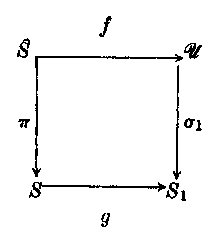
\includegraphics{chap06-vend-scan-03.eps}
\end{figure}

4) $\Gamma$ \emph{is essentially unique}. More precisely, we prove the following: \emph{if} $\Gamma_{1}\backslash \mathscr{U}=\Gamma_{2}\backslash \mathscr{U}=S$, \emph{then} $\Gamma_{1}=L\circ\Gamma_{2}\circ L^{-1}$, \emph{where} $L$ \emph{is a conformal homeomorphism of} $\mathscr{U}$. In fact, we have
\begin{equation*}
\Gamma_{i}=f_{i}\,\circ H\circ f_{i}^{-1},\qquad i=1,\,2
\end{equation*}
where $f_{1},\,f_{2}$ are conformal mappings of $\hat{S}$ on $\mathscr{U}$. Hence
\begin{equation*}
\Gamma_{2}=f_{2}\circ f_{1}^{-1}\circ (f_{1}\circ H\circ f_{1}^{-1})\circ f_{1}\circ f_{2}^{-1}=L\circ\Gamma_{1}\circ L^{-1},
\end{equation*}
where $L=f_{2} \circ f_{1}^{-1}$ and is obviously a conformal 1-1 mapping of $\mathscr{U}$ on itself.

We summarize our results in a


\begin{theorem*}
Let $S$ be a Riemann surface with hyperbolic\footnote{I.e., $\hat{S}$ is conformally equivalent to $\mathscr{U}$.} $\hat{S}$. Then $S$ is the quotient space\index{Riemann surface!as quotient space} $\Gamma\backslash \mathscr{U}$ of $\mathscr{U}$ by a group of linear transformations $\Gamma$, discontinuous in $\mathscr{U}$ and free of elliptic elements. $\Gamma$ is unique up to a similarity transformation $L\circ\Gamma\circ L^{-1}$ with $L$ a conformal self-mapping of $\mathscr{U}$.
$\Gamma$ is conjugate to the group of covering transformations of $\hat{S}$. Moreover, if $S$ is compact, $\Gamma$ is horocyclic \emph{(\ref{ch04:chap04}.~\ref{ch04:sec6A})} and its genus is greater than \emph{1}.
\end{theorem*}

The proof of the assertions in the last sentence is as follows. The compactness of $S$ implies (Theorem 3G) that $\bar{R}_{0}$ is compact in $\mathscr{U}$, which means that $\bar{R}_{0}$ is contained in a disk $|z|\leqq r<1$. Then $\Gamma$ is horocyclic (\ref{ch04:chap04}.~\ref{ch04:sec6E}). Now $R_{0}$ has a finite number of sides, $2n$, and a finite number of cycles, $c$. The cycles are all accidental, for $\Gamma$ has no fixed points. Thus the sum of the angles of $R_{0}$ is $2\pi c$ (cf. \ref{ch04:chap04}. Th. \ref{ch04:sec4C}). Let $P$ be the straight-sided polygon obtained by joining the vertices of $R_{0}$. The sum of the angles of $P$ is $2n(n-1)$. Since $R_{0}$ is convex and completely contained in $P$, it has a smaller angle sum. Applying \eqref{ch06:eqn10} we get
\begin{equation*}
0<2\pi(n-1)-2\pi c=2\pi(-c+n-1)=4\pi(g-1),
\end{equation*}
or $g>1$.

\subsection{}\label{ch06:sec3L} The group $\Gamma$ serves as a ``normal form'' for the Riemann surface $S$ in the sense that a class of conformally equivalent Riemann\index{Riemann surface!conformal equivalence of} surfaces $S$ is associated with a similarity class of groups\index{Riemann surface!group of conformal mappings of} $\Gamma$. The precise expression of this idea is found in the following theorem.


\begin{theorem*}
Two Riemann surfaces $S_{1}=\Gamma_{1}\backslash\mathscr{U}$ \emph{and} $S_{2}=\Gamma_{2}\backslash \mathscr{U}$ are conformally equivalent if and only if
\begin{equation*}
\Gamma_{1}=L\circ\Gamma_{2}\circ L^{-1}
\end{equation*}
with $L$ a conformal homeomorphism of $\mathscr{U}$.
\end{theorem*}

Suppose $\Gamma_{1}=L\circ\Gamma_{2}\circ L^{-1}$; we shall exhibit a mapping $f:S_{1}\rightarrow S_{2}$ with the desired properties.

Let $\sigma_{i}$ be the projection $\mathscr{U}\rightarrow\Gamma_{i}\backslash\mathscr{U},\,i=1,\,2$. Define
\begin{equation*}
f(p_{1})=\sigma_{2}\circ L^{-1}\circ\sigma_{1}^{-1}(p_{1}),\qquad p_{1}\in S_{1};
\end{equation*}
$f$ maps $S_{1}$ into $S_{2}$. By arguments similar to those of~\ref{ch06:sec3K}, \ref{ch06:sec3}) we are able to prove that $f$ is in fact a homeomorphism of the two surfaces. From $f\circ \sigma_{1}= \sigma_{2}\circ L^{-1}$ we can conclude that $f\circ \sigma_{1}$ is analytic, which, with the analyticity of $\sigma_{1}$, shows that $f$ is analytic. Hence $f$ is conformal, and one part of the theorem is demonstrated.

Assume, conversely, there is a 1-1 conformal map $f:S_{1}\rightarrow S_{2}$. Let $z_{0}\in \mathscr{U}$ and define $L(z_{0})=\sigma_{1}^{-1}\circ f^{-1}\circ\,\sigma_{2}(z_{0})$ by fixing a determination of $\sigma_{1}^{-1}$. $L$ is analytic in a neighborhood of $z_{0}$. We can continue $L$ analytically to any point of $\mathscr{U}$, the factors of $L$ being free of singularities on their domains. Since $\mathscr{U}$ is simply connected, the Monodromy Theorem assures us that $L(z)$ so defined is single-valued and regular in $\mathscr{U}$ (\ref{ch02:chap02}. \ref{ch02:sec7G}). In the same way we can define a function $M(z_{0})=\sigma_{2}^{-1}\circ f\circ \sigma_{1}(z_{0})$ and continue it throughout $\mathscr{U}$. If we fix the branch of $\sigma_{1}^{-1}$ at $z_{0}$ so that $L\circ M(z_{0})=z_{0}$, this relation will hold in all of $\mathscr{U}$. It is then proper to write $M=L^{-1}$. From the fact that both $L$ and $L^{-1}$ map $\mathscr{U}$ into $\mathscr{U}$, we conclude that $L$ is onto and therefore 1-1. Hence $L$ is a conformal homeomorphism of $\mathscr{U}$ on itself. Cf. Note 14, p. 401.

 Now suppose $V_{1}\in\Gamma_{1}$. Then
\begin{equation*}
\sigma_{2} \circ L^{-1}\circ V_{1}\circ L=f\circ \sigma_{1} \circ V_{1}\circ L=f\circ \sigma_{1}\circ L=\sigma_{2}\circ L^{-1}\circ L=\sigma_{2}.
\end{equation*}
Hence $L^{-1}\circ V_{1}\circ L\in\Gamma_{2}$, or $\Gamma_{1}\subset L\Gamma_{2}L^{-1}$. Similarly $V_{2}\in\Gamma_{2}$ implies $L \circ V_{2}\circ L^{-1}\in\Gamma_{1}$, or $L\circ\Gamma_{2}\circ L^{-1}\circ \Gamma_{1}$. This concludes the proof.

\begin{corollary*}
The group of\index{Hall, Marshall} conformal mappings of a Riemann surface\index{group of conformal mappings of a Riemann surface} $S$ on itself is isomorphic to the group $N_{\Omega} (\Gamma)/\Gamma$, where $N_{\Omega}(\Gamma)$ is the normalizer\index{normalizer} of $\Gamma$ in $\Omega$, the group of all conformal homeomorphisms of $\mathscr{U}$. \emph{(Note 17, p. 402.)}
\end{corollary*}

\skiptoctrue
\section*{Exercises}

1. Let $f,\,g$ be mappings of Riemann surfaces $S_{1}$ on $S_{2}$ and $S_{2}$ on $S_{3}$, respectively. If $g\circ f$ and $f$ are analytic, $g$ is analytic. Note that $f$ and $g$ need not be 1-1. [Use the identity
\begin{equation*}
\Phi_{3}\circ g\circ f\circ\Phi_{1}^{-1}=(\Phi_{3}\circ g\circ\Phi_{2}^{-1})\circ(\Phi_{2}\circ f\circ\Phi_{1}^{-1}),
\end{equation*}
where $\Phi_{i}$ is a disk homeomorphism of $S_{i},\,i=1,\, 2,\, 3$. Observe that the two factors of the right member are ordinary analytic functions.]

2. Give an example of a group $\Gamma$ having a finite number of fixed point classes whose Riemann surface is not compact.

[Construct the free product $G$ of an infinite number of hyperbolic\index{fixed point!hyperbolic} cyclic groups by the procedure of \ref{ch04:chap04}. Th. \ref{ch04:sec2B}. Show $G$ is a free group. The fundamental region of $G$ has an infinite number of sides.]

\section{Existence of Automorphic Functions and Forms}\label{ch06:sec4}\index{automorphic function!existence of}\index{Riemann surface!and automorphic functions}

Let $\Gamma$ be a function group with domain of existence $\mathscr{D}$ and let $S$ be the Riemann surface $\Gamma\backslash \mathscr{D}^{+}$. A meromorphic function (differential) on $S$ becomes an automorphic function (automorphic form) on $\mathscr{D}^{+}$. Since the existence of nonconstant functions and differentials on arbitrary Riemann surfaces is known (Section~\ref{ch06:sec2}), this gives another proof of the existence of nonconstant automorphic functions and forms on discontinuous groups (\ref{ch05:chap05}. Th. \ref{ch05:sec3E}).

\subsection{}\label{ch06:sec4A} We shall now prove these assertions.


\begin{theorem*}
Let $K=K(S)$ be the field of meromorphic functions \index{Riemann surface!field of functions on}on $S$ and $\mathbf{K} =\mathbf{K}(\Gamma)$ the field of automorphic functions\index{automorphic function!field of\_\_\_s} on $\Gamma$. Then $K$ is isomorphic to $\mathbf{K}$ by the mapping $f\leftrightarrow\varphi,\,f\in \mathbf{K},\,\varphi\in K$, where
\begin{equation}
\label{ch06:eqn11} f(x)=\varphi(q),\qquad x\in \mathscr{D}^{+},\qquad q=\sigma x \in S,
\end{equation}
$\sigma$ being the mapping $\mathscr{D}^{+}\rightarrow\Gamma\backslash \mathscr{D}^{+}$
\emph{(cf.~\ref{ch06:sec3B})}. Moreover \emph{(\ref{ch06:sec2A};~\ref{ch05:chap05}.~\ref{ch05:sec4A})}
\begin{equation}
\label{ch06:eqn12} n(x,\,f)=\eta(q,\, \varphi).
\end{equation}
\end{theorem*}

If $\varphi \in K,\,f(x)=\varphi(\sigma x)$ is defined for $x\in \mathscr{D}^{+}$ and
\begin{equation*}
f(Vx)=\varphi(\sigma(Vx))=\varphi(\sigma x)=f(x),\qquad V\in\Gamma
\end{equation*}
so that $f$ is invariant on $\Gamma$. Let $\zeta$ be a local variable at $q$; for $p$ near $q$ we have the expansion (we assume $\zeta(q)=0$)
\begin{equation*}
\varphi(p)=\sum\limits_{n=\mu}^{\infty}a_{n}\zeta^{n},\qquad \mu=\eta(q,\,\varphi).
\end{equation*}
A change of local variable would not affect $\mu$ (cf.~\ref{ch06:sec2A}).

But if we choose for $\zeta$ the variable $\Phi_{x}$ defined in (\ref{ch06:eqn9a}, b, c), $\Phi_{x}=\tau_{x}\circ\sigma_{x}^{-1}$, we get from the above series, with $\sigma z =p,\,z$ near $x$,
\begin{equation*}
f(z)=\varphi(p)=\sum\limits_{n=\mu}^{\infty}a_{n}t^{n},
\end{equation*}
where $t=\tau_{x}(z)$ is the proper local variable for the expansion of an automorphic function (\ref{ch05:chap05}.~\ref{ch06:sec4A}). Hence $f$ is meromorphic on $\mathscr{D}^{+}$ and so $f\in \mathbf{K}$.

As a byproduct we have \eqref{ch06:eqn12}.

Conversely, if $f\in \mathbf{K}$, then $\varphi(q)=f(\sigma^{-1}(q))$ is single-valued because $f$ takes the same value at all points of $\sigma^{-1}(q)$. The above argument concerning the expansions is reversible, so $\varphi$ is meromorphic on $S$.

Since the mapping $f\leftrightarrow\varphi$ is obviously an isomorphism, the theorem is proved.

\begin{corollary*}
If $f$ and $\varphi$ correspond by the above isomorphism, then
\begin{equation*}
N(f)=N(\varphi)
\end{equation*}
\emph{(cf.~\ref{ch05:chap05}.~\ref{ch05:sec4G}.~\ref{ch06:chap06}.~\ref{ch06:sec2D})}. If $\Gamma$ is of genus 0, and only then, there exists a univalent automorphic function on $\Gamma$.
\end{corollary*}

$N(f)$ was defined to be the number of poles of $f$ in a fundamental set $R^{\ast}$. Now $\sigma$ is clearly 1-1 from $R^{\ast}$ to $S$ and we have just seen that the order of $f$ and $\varphi$ at $x$ and $\sigma x$ is the same. The second statement is an immediate consequence of Theorem 2K.

\subsection{}\label{ch06:sec4B}\begin{theorem*}  Let $H_{m}$ be the vector space\index{automorphic form!vector space of\_\_\_s} of meromorphic differentials\index{differential on a Riemann surface}\index{Riemann surface!space of differentials on} of weight $m$ on $S$, and let $\mathbf{H}_{m}$ be the vector space of automorphic forms of dimension $-2m$ on $\Gamma$. Then $H$ and $\mathbf{H}$ are isomorphic under the mapping $F\leftrightarrow d\Omega,\,F\in \mathbf{H}_{m},\,d\Omega \in H_{m}$, where
\begin{equation}
\label{ch06:eqn13} F\{x)(dx)^{m} =d\Omega(q),\qquad q=\sigma x.
\end{equation}
Moreover
\begin{align}
n(x,\,F)&=\eta(q,\, d\Omega),\nonumber\\
n(x,\,F)&=\eta(q,\,d\Omega)+m(1-1/l),\\
n(x,\,F)&=\eta(q,\,d\Omega)+m,\nonumber
\end{align}
according as $x$ is a nonfixed point, elliptic of order $l$, or a parabolic vertex.
\end{theorem*}


In particular, an \emph{abelian differential of the first kind} (i.e., an everywhere regular differential in $S$) corresponds to a \emph{cusp form of dimension} $-2$ (i.e., an automorphic form of dimension $-2$ which vanishes at all parabolic cusps of $\mathscr{D}^{+}$).

\begin{proof*}
Let $d\Omega$ be given. The definition \eqref{ch06:eqn13} shows that $F(x)(dx)^{m}$ is invariant under $\Gamma$. Let $d\Omega$ be represented locally by $g(\zeta)(d\zeta)^{m}$, where $\zeta$ is any local variable at $q$. Since $d\Omega$ is invariant to changes of local variable (\ref{ch06:sec2B}), we can use for $\zeta$ the variable $\Phi_{x}$ defined in (\ref{ch06:eqn9a}, b, c). Thus $d\Omega$ is an analytic function of $\zeta$. From the expansion of $g$ as a meromorphic function,
\end{proof*}\begin{equation*}
g(p)=\sum\limits_{n=\mu}^{\infty}a_{n}\Phi_{x}^{n},\qquad a_{\mu}\neq 0,\qquad
p\ \mathrm{near}\ q
\end{equation*}
and from $\Phi_{x}(p)=\tau_{x}\circ\sigma_{x}^{-1}(p)=\tau_{x}(z)=t$, we obtain:
\begin{equation*}
F(z)=g(t)\Big(\frac{dt}{dz}\Big)^{m}=\begin{cases}
a_{\mu}t^{\mu}+\cdots,\quad x\ \mbox{a nonfixed point}\\
(z-x^{\prime})^{-2m}t^{-m/l}\{b_{\mu}t^{m+u}+\cdots\},\quad b_{\mu}\neq 0,\\
\qquad x\ \mbox{an elliptic point of order}\ l\\
(z-x)^{-2m}t^{m}\{c_{\mu}t^{\mu}+\cdots \},\quad c_{\mu}\neq 0,\\
\qquad x\ \mbox{a parabolic vertex}.
\end{cases}
\end{equation*}
Here $x^{\prime}$ is the fixed point conjugate to $x$, and the expansions are valid for $z$ near $x$. Comparison with~\ref{ch05:chap05}.~\ref{ch05:sec4A} shows that $F$ is meromorphic in $\mathscr{D}^{+}$; hence $F\in \mathbf{H}_{m}$. Moreover we can read off formula (14).

Now suppose $F$ is given, $F\in \mathbf{H}_{m}$. Then $d\Omega(q)=F(\sigma^{-1}q)(d\sigma^{-1}q)^{m}$ is single-valued on $S$ because $F(x)(dx)^{m}$ takes the same value at all points $x\in \sigma^{-1}q$. The expansions for $d\Omega$ may be deduced from those of $F$ by reversing the above process, showing that $d\Omega$ is meromorphic on $S$. Thus $d\Omega\in H_{m}$.

The mapping \eqref{ch06:eqn13} is clearly an isomorphism of the vector spaces $\mathbf{H}_{m}$ and $H_{m}$. This completes the proof.

\subsection{}\label{ch06:sec4C} When $S$ is compact, we can use the Riemann-Roch theorem\index{Riemann-Roch theorem} to calculate the dimension of certain vector spaces of automorphic forms. As an example consider $\mathbf{C}^{+}=\mathbf{C}^{+} (\Gamma,\,-2m)$,
the space of automorphic forms $F$ of dimension $-2m$ that are regular at every point of $\mathscr{D}^{+}$, including the vertices.

First, if $m=0$, we are asking for the number of linearly independent automorphic functions that are regular everywhere. Because of the isomorphism between automorphic functions on $\Gamma$ and meromorphic functions on $S$ (cf.~\ref{ch06:sec4A}), this is the same as the number of linearly independent everywhere regular\index{automorphic form!space of everywhere regular\_\_\_s} functions on $S$. As we have seen, all such functions are constants (\ref{ch06:sec2E}). Hence
\begin{equation}
\label{ch06:eqn15} \dim \mathbf{C}^{+}(\Gamma,\, 0)=1.
\end{equation}

Now suppose $m\neq 0$. If $F_{0}$ is a fixed automorphic form of dimension
$-2m$, then $F/F_{0}=f$ is an automorphic function such that $fF_{0}$ is regular everywhere. Conversely, if $f$ is an automorphic function having this property, then $fF_{0}=F\in \mathbf{C}^{+}$. The mapping $F\rightarrow f$ is an isomorphism of $\mathbf{C}^{+}(\Gamma,\, -2m)$ and the space
\begin{equation*}
\mathbf{L} =\{f\in\{\Gamma,\,0\}|fF_{0}\ \mbox{is\ regular\ in}\ \mathscr{D}^{+}\}.
\end{equation*}
Hence $\dim \mathbf{C}^{+}=\dim \mathbf{L}$.

The condition $f\in \mathbf{L}$ is simply
\begin{equation*}
\tag{$\ast$} n(z,\,f)+n(z,\, F_{0})\geqq 0,\qquad z\in \mathscr{D}^{+}.
\end{equation*}

Let us now go over to the Riemann surface $S$. By the isomorphisms of Theorems~\ref{ch06:sec4A},~\ref{ch06:sec4B}, we have
\begin{equation*}
f\leftrightarrow\varphi,\qquad F_{0}\leftrightarrow d\Omega
\end{equation*}
and $(^{\ast})$ becomes, with $\sigma x =q$,
\begin{align*}
&\eta(q,\,\varphi)+\eta(q,\, d\Omega)\geqq 0,\qquad x= \mbox{nonfixed point},\\
&\eta(q,\,\varphi)+\eta(q,\,d\Omega)+m\Big(1-\frac{1}{l}\Big)\geqq 0,\quad
x=\mbox{elliptic point of order}\ l,\\
&\eta(q,\,\varphi)+\eta(q,\, d\Omega)+m\geqq 0,\quad x= \mbox{parabolic vertex}.
\end{align*}
If we make the convention
\begin{equation*}
\frac{1}{l(q)}=\frac{1}{l}=\begin{cases}
1,& q\quad \mbox{a nonfixed point},\\
0,& q\quad \mbox{a parabolic vertex}
\end{cases}
\end{equation*}
whereas for an elliptic fixed point $l$ retains its previous meaning, we can write one equation in place of the above three:
\begin{equation*}
\eta(q,\,\varphi)+\eta(q,\,d\Omega)+m\Big(1-\frac{1}{l}\Big)\geqq 0,\qquad
q\in S.
\end{equation*}
This may now be expressed in the following way. Set up the divisor
\begin{equation*}
D^{\ast}=\sum\limits_{q \in S}\Big[m\Big(1-\frac{1}{l}\Big)\Big]\cdot q
\end{equation*}
where $[x]$ denotes the largest integer $\leqq x$. Since the largest integer in a nonnegative number is nonnegative, it is clear that $f\in \mathbf{L}$ if and only if $\varphi$ is a multiple of
\begin{equation*}
D_{1}=D(-d\Omega)-D^{\ast}.
\end{equation*}
Thus
\begin{equation*}
\dim \mathbf{C}^{+}(\Gamma,\,-2m)=\dim \mathbf{L}=\dim D_{1}.
\end{equation*}

Now since $d\Omega$ is a differential of weight $m$, we have
\begin{equation}
\begin{split}
\deg D_{1} & =\deg D(-d\Omega)-\deg D^{\ast}\\
&=-2m(g-1)-\sum\Big[m\Big(1-\frac{1}{l_{i}}\Big)\Big],
\end{split}\label{ch06:eqn16}
\end{equation}
where we now sum only over the elliptic and parabolic cycles, the other terms being zero.

\emph{At this point we assume} $\Gamma$ \emph{is horocyclic} (\ref{ch04:chap04}.~\ref{ch04:sec6A}). From~\ref{ch05:chap05}. \eqref{ch05:eqn29} we deduce
\begin{equation}
\label{ch06:eqn17} g\,-1+\frac{1}{2}\sum\limits_{i}\Bigg(1-\frac{1}{l_{i}}\Bigg)>0,
\end{equation}
since the left member is $J/2m$, which is positive by~\ref{ch05:chap05}. \eqref{ch05:eqn27}. ($J$ is the sum of the orders of an automorphic form of dimension $-2m$ in a fundamental set.)

There are several cases.

1) $m < 0$. Since $-[x]\geqq-x$,
\begin{equation*}
\deg D_{1}\geqq-2m\;\Bigg\{g-1+\frac{1}{2}\sum\Bigg(1-\frac{1}{l_{i}}\Bigg)\Bigg\}>0,
\end{equation*}
by \eqref{ch06:eqn17}. Hence (\ref{ch06:sec2H}) we have $\dim D_{1}=0$ and so $\dim \mathbf{L}=0$. That is, everywhere regular nonconstant automorphic forms of (even integral) positive dimension do not exist. This is the result we got in \ref{ch05:chap05}. Th. \ref{ch05:sec4J} (for all integral positive dimensions).

2) $m>0$. The Riemann-Roch theorem gives
\begin{equation*}
\tag{$\dagger$} \dim D_{1}=-\deg D_{1}-g+1+\dim\ (-D_{1}-Z).
\end{equation*}
Again
\begin{equation*}
\deg\ (-D_{1}-Z)=2(m-1)(g-1)+\sum\limits_{i}\Bigg[m\Bigg(1-\frac{1}{l_{i}}\Bigg)\Bigg],
\end{equation*}
since $\deg(-Z)=-2(g-1)$. Denote by $\sigma_{0}$ and $e_{0}$ the number of inequivalent parabolic and elliptic fixed points, respectively.


\begin{lemma*} For $m\geqq 1,\,l\geqq 1$, we have
\begin{equation*}
\Bigg[m\Bigg(1-\frac{1}{l}\Bigg)\Bigg]\geqq(m-1)\Bigg(1-\frac{1}{l}\Bigg).
\end{equation*}
\end{lemma*}

\noindent With the obvious case $l=1$ disregarded, the result is equivalent to
\begin{equation*}
\frac{m}{l}+\Big[-\frac{m}{l}\Big]\geqq\frac{1}{l}-1.
\end{equation*}
Since the left member is periodic in $m$ with period $l$. we may assume $1\leqq m\leqq l$. Then $[-m/l]=-1$ and the inequality reduces to
\begin{equation*}
\frac{m}{l}\geqq \frac{1}{l}.
\end{equation*}

Using the lemma in the equation following $(\dagger)$, we get
\begin{equation*}
\deg(-D_{1}-Z)\geqq(m-1)\ \Big\{2(g-1)+\sum\Big(1-\frac{1}{l_{i}}\Big)\Big\},
\end{equation*}
and this is certainly positive when $m>1$ because of \eqref{ch06:eqn17}. Moreover, when $m=1$. we have, from the equation following $(\dagger)$,
\begin{equation*}
\deg(-D_{1}-Z)=\sum\limits_{i}\bigg(1-\frac{1}{l_{i}}\bigg)=\sigma_{0}.
\end{equation*}

Thus for all $m>1$ and for $m=1,\,\sigma_{0}>0$, we see that $\deg(-D_{1}-Z) >0$, implying $\dim(-D_{1}-Z)=0$ (cf. \ref{ch06:sec2H}). Hence:

\begin{theorem*}
Let $\Gamma$ be a horocyclic group with compact Riemann surface. Let $\sigma_{0}$
be the number of inequivalent parabolic vertices of $\Gamma$. We assume $\sigma_{0}\geqq 0,\,m\geqq 1$, and $m+\sigma_{0}>1$. Then the dimension of the space $\mathbf{C}^{+}(\Gamma,\, -2m)$ of everywhere regular automorphic forms of even integral dimension $-2m$ is given by:
\begin{equation*}
\dim \mathbf{C}^{+}(\Gamma,\, -2m)=\begin{cases}
1,\quad m=0,\\
0,\quad m<0,\\
(2m-1)(g-1)+\sum\limits_{i}\bigg[m\bigg(1-\frac{1}{l_{i}}\bigg)\bigg],\quad
m>0
\end{cases}
\end{equation*}
where the sum is extended over all cycles of a fundamental region.
\end{theorem*}

The case we had to exclude is $m=1,\,\sigma_{0}=0$. The everywhere regular forms in $\{\Gamma,\,-2\}$ include the cusp forms, and a cusp form corresponds to an everywhere regular differential on $S$. Since there are $g$ of those, we have
\begin{equation*}
\dim C^{+}(\Gamma,\,-2)\geqq g.
\end{equation*}

This theorem is actually true for all function groups with compact Riemann surfaces. We used the hypothesis that $\Gamma$ is horocyclic only to deduce \eqref{ch06:eqn17}. We can, however, prove \eqref{ch06:eqn17} for an arbitrary function group as follows. Let $d\Omega$ be a differential of weight 1 and $F$ the corresponding automorphic form. Then
\begin{equation*}
\deg d\Omega=2g-2=\sum\limits_{q\epsilon S}\eta(q,\,d\Omega)=\sum\limits_{z\in
R^{\ast}}n(z,\,F)-\sum \bigg(1-\frac{1}{l_{i}}\bigg),
\end{equation*}
and we know from \ref{ch05:chap05}. Th. \ref{ch05:sec4E} that
\begin{equation*}
\sum n(z,\,F)>0.
\end{equation*}

\section{The Algebraic Field of Automorphic Functions}\label{ch06:sec5}

In this Section we shall study $\mathbf{K}(\Gamma)$, the field of automorphic functions on $\Gamma$, when the associated Riemann surface is compact. We shall derive the properties of $\mathbf{K}$ from those of $K(S)$), the field of meromorphic functions on $S=\Gamma\backslash \mathscr{D}^{+}$, by utilizing the isomorphism of the two fields (Theorem~\ref{ch06:sec4A}). Since the theorems needed about $K(S)$ are very well known, their statement, with references, will be sufficient. We emphasize that in these developments the restriction to compact surfaces is essential.

\subsection{}\label{ch06:sec5A} Let $S$ be a compact Riemann surface. We have seen that every (meromorphic) function $\varphi$ on $S$ has a definite valence $N$, that is, $\varphi$ assumes each complex value $N$ times (\ref{ch06:sec2E}).


\setcounter{theorem}{0}
\begin{theorem}\label{ch06:thm1} Any two functions $\varphi,\,\psi$ \emph{on} $S$ satisfy an irreducible algebraic equation $P=0$, where $P$ is a polynomial in two indeterminates with complex coefficients. $P$ is of degree $\leqq N(\psi)$ in $\varphi$ \emph{(}and of degree $\leqq N(\varphi)$ in $\psi$\emph{)}.
\end{theorem}

\begin{theorem}\label{ch02:thm2b}
Corresponding to each $N$-valent $\psi\in K(S)$ there is a $\varphi\in K(S)$ such that the above irreducible polynomial $P$ is of the exact degree $N$ in $\varphi$. $K(S)$ is generated by any pair $(\varphi,\,\psi)$ satisfying these requirements. In other words, every function in $K(S)$ is a rational function of $\varphi$ and $\psi$.
\end{theorem}

For the proofs cf. \citeauthor{Ahlfors0000a}\index{Ahlfors-Sario} [\ref{Ahlfors}, Ths. 25C, 25D, pp. 322--323]; \citeauthor{Springer0000}~[\ref{Springer1},\index{Springer} Th. 10--26, p. 289].

An algebraic function field\index{automorphic function!algebraic function field of \_\_\_s} of a single complex variable is the set of all rational functions of $x$ and $y$, where $x,\,y$ satisfy an irreducible algebraic equation $Q(x,\,y)=0$ with complex coefficients. Therefore the last theorem can be restated:

\begin{theorem}\label{ch03:thm3}
$K(S)$ is isomorphic to an algebraic function field of one variable.
\end{theorem}

\subsection{}\label{ch06:sec5B} We now use the isomorphism of Theorem~\ref{ch06:sec4A} to translate the theorems of~\ref{ch06:sec5A} into theorems about automorphic functions. Let $f,\, g\in \mathbf{K}(\Gamma)$. Suppose, under the isomorphism, $f\rightarrow\varphi,\,g \rightarrow\psi;\varphi,\,\psi\in K(S)$. By Corollary~\ref{ch06:sec4A},
$N(\psi)=N(g)$. There is an equation $P=0$ satisfied by $\varphi,\,\psi$ and $P$ is of degree $\leqq N(\psi)$ in $\varphi$. Since the isomorphism obviously leaves constants individually fixed, it maps $P(\varphi,\, \psi)$ onto $P(f,\, g)$. Hence (\ref{ch05:chap05}. Th. \ref{ch05:sec6A}):


\begin{theorem*}
Let $\Gamma$ be a function group on $\mathscr{D}$ such that the Riemann surface $\Gamma\backslash \mathscr{D}^{+}=S$ is compact. Then any two automorphic functions $f$ and $g$ satisfy an irreducible algebraic equation $P= 0$ with complex coefficients. $P$ is of degree $\leqq N(g)$ in $f$.
\end{theorem*}

\subsection{}\label{ch06:sec5C} From Theorems 2, 3 of 5A we obtain immediately:


\begin{theorem*}
$\mathbf{K}(\Gamma)$ is generated by any two automorphic functions $f,\,g$ which are such that the irreducible equation they satisfy is of degree $N(g)$ in $f$. There are always two such functions. $\mathbf{K}(\Gamma)$ is isomorphic to an algebraic function field\index{automorphic function!algebraic function field of\_\_\_s} of one variable.
\end{theorem*}

\subsection{}\label{ch06:sec5D} The following result is more special.


\begin{theorem*}
There are two automorphic functions\index{automorphic function!algebraic function field of\_\_\_s}, each the quotient of Poincar\'{e} series\index{Poincar\'{e} series}, which generate $\mathbf{K}(\Gamma)$.
\end{theorem*}

We must first prove a lemma which puts the condition of irreducibility in a more tractable form. Cf. Note 16, p. 402.

\begin{lemma*}
Let $R^{\ast}$ be a fixed fundamental set of $\Gamma$. For any complex number $g_{0}$ and any $g\in \mathbf{K}$, denote by $\{z_{i}(g_{0}),\,i=1,\,2,\,\cdots,\,N(g)\}$ the points in $R^{\ast}$ where $g(z)=g_{0}$. Then the irreducible equation
$P(f,\,g)=0$ satisfied by $f,\,g \in \mathbf{K}$ is of degree $N=N(g)$ in $f$ if there is a complex number $g_{0}$ such that
\begin{enumerate}
\item[1)] the points $\{z_{i}(g_{0}),\, i=1,\,\cdots,\,N\}$ are distinct,
\item[2)] the values $\{f(z_{i}(g_{0})),\, i=1,\ldots,\,N\}$ are distinct.
\end{enumerate}
\end{lemma*}

For the equation $P(f,\,g_{0})$ has the $N$ distinct roots $f(z_{i}(g_{0})),\,\cdots,\, f(z_{N}(g_{0}))$ and therefore is of degree $\geqq N$ in $f$. On the other hand we knew it was of degree $\leqq N$ (Theorem~\ref{ch06:sec5B}).\:\:\:q.e.d.

To prove the theorem we take any two Poincar\'{e} series whose quotient is an automorphic function; denote this function by $g(z)$ (cf.~\ref{ch05:chap05}.~\ref{ch05:sec3C}). Consider the set $A$ consisting of those $z\in R^{\ast}$ for which $g^{\prime}(z)=0$. This is clearly a countable set since $g^{\prime}$ is meromorphic. Hence the set $g(A)=\{g(z)|z\in A\}$ is likewise countable. If we now choose $g_{0}\not\in g(A)$, the set $z_{i}(g_{0}),\, i= 1,\, 2, \cdots,\,N$, will consist of distinct points. Thus 1) is satisfied.

Define the Poincar\'{e} series
\begin{equation*}
F(z,\,\lambda)=\sum\limits_{V\epsilon\Gamma}\bigg(\frac{dVz}{dz}\bigg)^{2}\frac{1}{\lambda-Vz}.
\end{equation*}
Considered as a function of $\lambda,\,F$ is meromorphic in the whole plane, having poles at the points $\lambda=Vz,\, V\in\Gamma$. (These poles are simple provided $z$ is not a fixed point.) Hence, for fixed $z,\,F$ has a countable set of zeros in $\lambda$. We can therefore choose $\lambda_{0}$ so that
\begin{equation*}
F(z_{i},\,\lambda_{0})\neq 0, \infty;\qquad i=1,\,2,\cdots,N.
\end{equation*}

Next choose $\lambda_{1}$ so that
\begin{equation*}
\frac{F(z_{i},\,\lambda_{1})}{F(z_{i},\,\lambda_{0})}\neq\frac{F(z_{j},\,\lambda_{1})}{F(z_{j},\,\lambda_{0})},\qquad
i\neq j,\qquad i,\,j=1,\,2,\cdots,\,N.
\end{equation*}
This is possible. Indeed, the equality of the above quantities would imply
\begin{equation*}
\frac{F(z_{i},\,\lambda_{1})}{F(z_{j},\,\lambda_{1})}=\frac{F(z_{i},\,\lambda_{0})}{F(z_{j},\,\lambda_{0})},\qquad
i\neq j.
\end{equation*}
But the left member is the value, at $\lambda=\lambda_{1}$, of a meromorphic function $h_{ij}(\lambda)$ which is no constant, for it becomes infinite at $\lambda=z_{j}$. Hence a number $\lambda_{1}$ can be found so that for each $i\neq j,\,1\leqq i,\,j\leqq N,\,h_{ij}$ avoids the right member. (The right member is a constant---depending on $i,\,j$---since $\lambda_{0}$ has already been chosen.) It follows that
\begin{equation*}
f(z)=F(z,\,\lambda_{1})/F(z,\,\lambda_{0})
\end{equation*}
is a function in $\mathbf{K}(\Gamma)$ which satisfies condition $2)$ of the lemma. The equation satisfied by $f$ and $g$ is therefore of degree $N(g)$ in $f$, and by Theorem~\ref{ch06:sec5C} this means $f$ and $g$ generate $\mathbf{K}(\Gamma)$.

%%%%%%%%%chapter07

\chapter{The Structure of Discontinuous Groups}\label{ch07:chap07}\index{automorphic functions of $n$ variables}


\section{Generation of Principal-Circle Groups by Geometrical and Number-Theoretical Methods}\label{ch07:sec1}

So far we have mostly assumed the existence of discontinuous groups and on this basis have derived their properties. It is true that the method of free products (\ref{ch04:chap04}. \ref{ch04:sec2}) permits us to construct a wide variety of groups. But no horocyclic group (\ref{ch04:chap04}. \ref{ch04:sec6A}) containing elliptic fixed points (e.g. the modular group) can be constructed by this method. Again, we can define discontinuous groups as covering groups of Riemann surfaces (\ref{ch06:chap06}. \ref{ch06:sec3K}). But we obtain in this way only groups without elliptic elements. Even if by these methods the existence of a discontinuous group is demonstrated, we still get no information about the group itself: no method is given to determine its generators or the coefficients of its matrix representation. Finally, a serious objection to both of these methods is the fact that they afford no insight into the totality of groups which they generate, or how this totality compares with the totality of all discontinuous groups.

Poincar\'{e} attacked this problem in his earliest detailed expository paper (\citeauthor{Poincare0000}~[\ref{Poincare1}, pp. 108--168]) and solved it in the most important special case: he showed that \emph{the class of principal-circle groups with finitely-sided fundamental regions is coextensive with the class of noneuclidean polygons satisfying certain conditions}. As we have seen (\ref{ch06:chap06}. \ref{ch06:sec3F}), a group of this class determines a compact Riemann surface, and conversely. Poincar\'{e}'s result is therefore a characterization of the totality of principal-circle groups that are associated with compact Riemann surfaces.

There is another interpretation, more geometrical, of Poincar\'{e}'s theorem. Since the unit disk is a model of the hyperbolic plane, each partition of the disk into fundamental regions may be regarded as a tessellation of the hyperbolic plane by a group of (directly conformal) rigid motions. The theorem under discussion describes all possible tessellations into polygons with a finite number of sides.

There is still another method of generating principal-circle groups, one that is arithmetical in nature, which will be described in 1H. This method is important because it is the only method presently known to be capable of generalization to higher dimensional space.

\subsection{}\label{ch07:sec1A}
(Cf. Note 17a, p. 403.) We consider principal-circle groups defined on $\mathscr{U}$, the interior of the unit circle $\mathscr{Q}$. Let $\Gamma$ be \emph{horocyclic} (\ref{ch04:chap04}. \ref{ch04:sec6A}). The elements of $\Gamma$ are linear transformations\index{construction of principal-circle group!by geometrical method|(} that preserve $\mathscr{U}$.\index{generalized unit disk $=\mathfrak{U}$} We assume $\Gamma$ has a normal polygon $N_{0}$ with a finite number of sides. $N_{0}$ is a \emph{polygon} (\ref{ch04:chap04}. \ref{ch04:sec7D}) and has the following properties (\ref{ch04:chap04}. \ref{ch04:sec7E} and \ref{ch04:sec7C}, Lemma \ref{ch04:lem4}):


1) The boundary of $N_{0}$ consists of a finite number of pairs of sides $(s_{i},\,s_{i}^{\prime})$. There is a unique element $T_{i}\in\Gamma$ which maps $s_{i}$ on $s_{i}^{\prime}$ and maps the exterior of the circle\footnote{If $s_{i}$ lies on a diameter, replace ``exterior'' by ``one side,'' etc.} on which $s_{i}$ lies on the interior of the circle on which $s_{i}^{\prime}$ lies.

2) The sum of the angles at the vertices of an elliptic cycle of order $l$ is $2\pi/l$.

3) The sum of the angles at the vertices of an accidental cycle lying in $\mathscr{U}$ is $2\pi$.

4) $N_{0}$ can be chosen so that its boundary meets $\mathscr{Q}$ in at most a finite number of parabolic vertices; in particular, there are no accidental vertices of the first kind on $\mathscr{Q}$. Cf. \ref{ch04:chap04}. \ref{ch04:sec7G}.


Poincar\'{e}\index{Poincar\'{e}} showed that these conditions are \emph{sufficient}: each polygon satisfying 1)--4) is the fundamental region of a horocyclic group.

We now \emph{start} with a polygon $P_{0}$ bounded by a finite number of pairs of sides $(s_{i}, s_{i}^{\prime}),\,i=1,\,\cdots,\,n$, where $s_{i}$ is noneuclidean congruent to $s_{i}^{\prime}$. It follows that there is a linear transformation $T_{i}$ preserving $\mathscr{U}$ that maps $s_{i}$ on $s_{i}^{\prime}$ and maps the outside of the circle determined by $s_{i}$ on the inside of the circle determined by $s_{i}^{\prime}$. We then \emph{define} $\Gamma$ to be
\begin{equation*}
\Gamma=\{T_{1},\,T_{2},\,\cdots,\,T_{n}\},
\end{equation*}
i.e., $\Gamma$ is the group generated by $\{T_{i}\}$.

Let
\begin{equation}\label{ch07:eqn1}
\mathfrak{T}=\bigcup_{i= 1}^{n}\,(T_{i},\,T_{i}^{-1}).
\end{equation}
Each element of $\Gamma$ is a word in $\mathfrak{T}$. $\Gamma$ is a countable group. Every element of $\Gamma$ preserves $\mathscr{U}$ and has at most two fixed points in $\mathscr{U}$. A vertex of $P_{0}$ may or may not be a fixed point; in either case it determines a cycle in $P_{0}$, namely, the set of points in $\overline{P}_{0}$ to which it is equivalent under $\Gamma$. We can therefore speak of elliptic, accidental, and parabolic cycles. Obviously each point of a cycle is also a vertex, since $P_{0}$ is a polygon. Conditions 2)--4) are therefore meaningful.

We see that each point of an elliptic cycle is an elliptic fixed point and lies in $\mathscr{U}$. The points of a parabolic cycle lie on $\mathscr{Q}$.

\emph{From now on assume} $P_{0}$ \emph{satisfies} 2)--4). \emph{It automatically satisfies} 1).


\subsection{}\label{ch07:sec1B} Let $\{V_{i,}\,i=0,1,2,\,\cdots\}$ be an enumeration of the elements of $\Gamma$ and let $P_{i}=V_{i}(P_{0})$. In order to show $P_{0}$ is a fundamental region for $\Gamma$ it is sufficient to prove two things:

A) $P_{i}$ and $P_{j}$ are either disjoint or identical.

B) $\Gamma\overline{P}_{0}$ covers $\mathscr{U}$.


The existence of a fundamental region with inner points will show that $\Gamma$ is discontinuous (\ref{ch04:chap04}. IB).

\subsection{}\label{ch07:sec1C}
We prove A) first. We shall exhibit a subcollection of polygons of $\Gamma P_{0}$ which are mutally disjoint. These polygons will be assembled in successively larger rings called \emph{generations}\index{polygon of generation $m$}. Then we shall show that every polygon of $\Gamma P_{0}$ is in some generation.

Let $\alpha=\alpha_{1}$ belong to an ordinary cycle of $P_{0}$. We use the method of \ref{ch04:chap04}. \ref{ch04:sec4G} to get the remaining vertices $\alpha_{2},\,\cdots,\,\alpha_{t}$ of the cycle. The argument there did not require $\Gamma$ to be discontinuous; all that was needed was the existence of transformations $W_{j}$ such that $W_{j}\alpha_{j}=\alpha_{j+1},\,j=1,\,\cdots,\,t-1$; $W_{t}\alpha_{t}=\alpha_{1}$. Now $\alpha_{j}$ is the initial point of a side $s_{j}$ whose conjugate side $s_{j}^{\prime}$ ends in $\alpha_{j+1}$; the existence of $W_{j}$ then follows because $P_{0}$ satisfies condition 1) of 1A, and in fact $W_{j}\in \mathfrak{T}$.

\begin{figure}[!h]
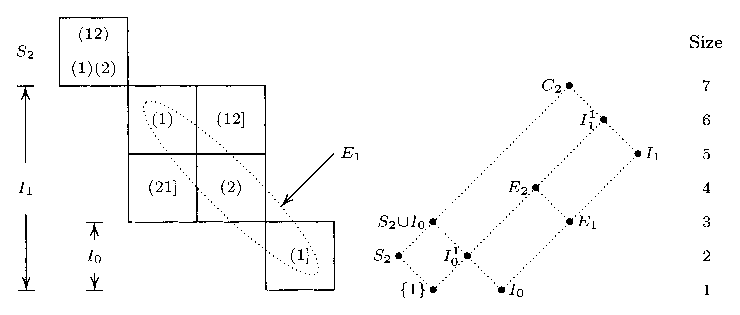
\includegraphics{chap07-vend-scan-01.eps}
\end{figure}

The transformation $W_{t}W_{t-1}\cdots W_{i}$ maps a small triangular region lying in $P_{0}$ with apex at $\alpha_{i}$ on a small triangular region with vertex at $\alpha_{1}$ lying outside of $P_{0}$. In fact, $W_{t}\cdots W_{i}$ maps $P_{0}$ on a polygon $P_{i}^{\prime}$ having a vertex at $\alpha_{1}$:
the polygons appear in the counterclockwise order $P_{t}^{\prime},\,P_{t-1}^{\prime},\, \cdots, P_{1}^{\prime}$.

If the cycle is accidental, then by hypothesis the sum of the angles at the vertices $\{\alpha_{i}\}$ is $2\pi$. Since the transformations involved are conformal, this means that the sum of the angles in the polygons $P_{t}^{\prime},\,\cdots,\,P_{1}^{\prime}$ is $2\pi$, or one side of $P_{1}^{\prime}$ lies along $s_{t}^{\prime}$. It follows that the transformation $W_{t}\cdots W_{1}$ is the identity and $P_{1}^{\prime}$ coincides with $P_{0}$. If, on the other hand, the cycle is elliptic then $P_{1}^{\prime}\neq P_{0}$, for the sum of the angles at the vertices of the cycle equals $2\pi/l,\,l>1$. The transformation $E=W_{t}\cdots W_{1}$ maps $\alpha_{1}$ on itself and so is elliptic, since it is not the identity. The complete neighborhood of $\alpha_{1}$ is covered by $l-1$ applications of $E$ to the elliptic sector at $\alpha_{1}$ obtained by intersecting $\bigcup_{1}^{t}P_{i}^{\prime}$ and a small disk with center at $\alpha_{1}$.

The $P_{i}^{\prime}$ do not intersect each other or $P_{0}$. Indeed, note that $P_{0}$ is bounded at $\alpha_{1}$ by the sides $s_{1}$ and $s_{t}^{\prime}$. Let us speak indifferently of the arc $s_{j}$ and of the circle on which it lies, calling them both $s_{j}$. Then $P_{0}$ is outside $s_{j}^{\prime}$. Now $P_{t}^{\prime}$ is inside $s_{j}^{\prime}$ and so does not meet $P_{0}$. Let $s_{t-1}^{\ast}$ be the other boundary of $P_{t}^{\prime}$ at $\alpha_{1}$. Then $P_{t-1}^{\prime}$ is inside $s_{t-1}^{\ast}$ and cannot meet $P_{t}^{\prime}$ or $P_{0}$. Continuing in this way, we prove the assertion.

Secondly, suppose $\alpha$ is a vertex of $P_{\dot{0}}$ lying on $\mathscr{Q}$. Then $\alpha$ is parabolic, because $P_{0}$ satisfies 4) of 1A. Applying the above method to $\alpha$ and the side $s_{1}$ beginning at $\alpha$, we return to $\alpha$ by a side $s_{t}^{\prime}$ in $t$ steps. $\alpha=\alpha_{1}$ is an element of the parabolic cycle $\alpha_{1},\,\cdots,\,\alpha_{t}$. By the reasoning of \ref{ch04:chap04}. \ref{ch04:sec4G} we find that $P_{0}$ is bounded at $\alpha$ by $P^{\prime}=W_{t}P_{0}$ and $P^{\prime\prime}=W_{1}^{-1}P_{0}$ and that the 3 polygons are distinct. (Notation same as before.)

Finally, if $\alpha$ is an inner point of a side $s$, and $s^{\prime}$ is the conjugate side, then the mapping which sends $s^{\prime}$ into $s$ sends $P_{0}$ into a polygon $P^{\prime}$ which borders $P_{0}$ along $s$. $P_{0}$ and $P^{\prime}$ are disjoint, since $P_{0}$ is outside, $P^{\prime}$ inside, $s$.

We have seen that the neighborhood of each point on the boundary of $P_{0}$ is covered by disjoint polygons $\{P_{i}\}$. Now let us see how these polygons fit together. Let $\alpha$ be an ordinary vertex and let us describe the boundary of $P_{0}$ counterclockwise, beginning at $\alpha$. We encounter a side $s$ with initial point $\alpha$. Among the polygons which form a ring around $\alpha$ there is one, $P^{\prime}$, which borders $P_{0}$ along $s$. The method of construction described above shows that the side of $P^{\prime}$ which lies along $s$ actually coincides with $s$. Hence, if $\beta$ is the other endpoint of $s,\,P^{\prime}$ is one of the polygons ringing $\beta$. We now fill in the polygons which lie counterclockwise from $P^{\prime}$ and have a vertex at $\beta$, ending with a polygon $P^{\prime\prime}$ which borders $P_{0}$ along $s_{1}$, the other side issuing from $\beta$. This process can be continued, with obvious modifications in the case of parabolic vertices, until we return to $\alpha$ and the polygon $P^{\prime}$.

$P$ will be called a polygon of generation 1 if it is not $P_{0}$ and if it has been obtained by applying the above process to a vertex of $P_{0}$. Such a polygon has at least a vertex in common with $P_{0}$. (But there may be other polygons in $\Gamma P_{0}$ having a vertex in common with $P_{0}$ which cannot be obtained in this way; if such polygons exist, they are not first generation.) In general, $P$ is of generation $m$ if it is not of lower generation and if it has been obtained by applying the above process to a vertex of a polygon of generation $m-1$. $P_{0}$ is the unique polygon of generation $0$. We let $G_{m}$ stand for the set of polygons of generation $m$. We also define
\begin{equation*}
F_{m}=\bigcup_{k=0}^{m}G_{k}.
\end{equation*}
Obviously $F_{0}\subset F_{1}\subset \cdots$. Also, $F_{m}$ is a finite set, for the polygons having a vertex in common with a given polygon are, at each stage of the process, finite in number.

What we have shown is that the polygons of $G_{1}$ form a complete ring about $P_{0}$ (with an obvious interpretation at parabolic vertices) and that $F_{1}$ is a disjoint collection of polygons.


\subsection{}\label{ch07:sec1D}
We now wish to show that $F_{m}$ is a disjoint collection for each $m$.

We have seen that $P_{0}$ is disjoint\index{generalized unit disk $=\mathfrak{U}$!analytic automorphisms of} from all $P\in G_{1}$ and that the polygons of $G_{1}$ form a complete ring about $P_{0}$ in the sense that their closures cover a neighborhood of $P_{0}$. The outer boundaries of the polygons of $G_{1}$ make up the boundary of a polygon $\Pi$ which contains $P_{0}$ in its interior. The method of construction shows that each $P\in G_{2}$ lies outside $\Pi$ and so cannot meet $P_{0}$. By induction one establishes the same property for $G_{m}$. Thus we can say that $P_{0}$ \emph{and} $P\in F_{m}$ \emph{are disjoint or identical for} $m=0,1,2,\,\cdots$.

Now each $P\in F_{m}$ is of the form $VP_{0}$, where
\begin{equation*}
\tag{$\ast$} V=T_{i_{1}}T_{i_{2}}\cdots T_{i_{k}},\qquad T_{i}, \in \mathfrak{T};
\end{equation*}
the $T$'s are not necessarily distinct (cf. \ref{ch06:sec1A}). To see this, draw a straight line $\lambda$ connecting a point in $P_{0}$ with a point in $P$. This line can be shifted slightly to avoid passing through vertices of polygons in $F_{m}$. Let $\lambda$ leave $P_{0}$ by the side $s_{1}^{\prime};\,\lambda$ next enters the contiguous polygon $T_{i_{1}}(P_{0})=P_{1}$, where $T_{i_{1}}s_{1}=s_{1}^{\prime}$ and $s_{1},\,s_{i}^{\prime}$ are conjugate sides of $P_{0}$. Then $P_{1}\in F_{1}$. Suppose $\lambda$ leaves $P_{1}$ by the side $s_{2}^{\prime}$ and let $T_{i_{1}}$ map $T_{i_{1}}^{-1}s_{2}$ on $T_{i_{1}}^{-1}s_{2}^{\prime}$; $\lambda$ next enters $T_{i_{1}}T_{i_{2}}T_{i_{1}}^{-1}P_{1}=T_{i_{1}}T_{i_{2}}P_{0}=P_{2}$, and $P_{2}\in F_{2}$. In a finite number of steps we arrive at $P$, and $(^{\ast})$ follows.

Conversely, each $P$ of the form $VP_{0}$ lies in $F_{m}$ for some $m$. In fact, by a reversal of the above reasoning, we get
\begin{equation*}
T_{i_{1}}P_{0}=P_{1}\in F_{1},\qquad\quad T_{i_{1}}T_{i_{2}}P_{0}=T_{i_{1}}T_{i_{2}}T_{i_{1}}^{-1}P_{1}=P_{2}\in F_{2},
\end{equation*}
and
\begin{equation*}
T_{i_{1}}T_{i_{2}}\cdots T_{i_{k}}P_{0}=P_{k}\in F_{k}.
\end{equation*}

Suppose $P$ and $Q$ are two polygons in $F_{m}$ that intersect. We have
\begin{equation*}
P=UP_{0}=S_{1}S_{2}\cdots S_{r}P_{0},\qquad Q=VP_{0}=W_{1}W_{2}\cdots W_{s}P_{0},
\end{equation*}
where $S_{i},\,W_{i}\in \mathfrak{T}$. Then $U^{-1}P=P_{0}$ meets $U^{-1}VP_{0}$. But $U^{-1}V= S_{r}^{-1}\cdots S_{1}^{-1} W_{1}W_{2}\cdots W_{s}$ is of the form $(^{\ast})$; hence $R=U^{-1}VP_{0}$ is a polygon in some $F_{m}$ and $R$ meets $P_{0}$. It follows that $R=P_{0}$, or $P=Q$.

We have shown that $F_{m}$ is a disjoint collection of polygons. But every polygon of $\Gamma P_{0}$ is in some $F_{m}$. For, if $P\in\Gamma P_{0}$, we have $P=VP_{0}$, with $V$ of the form $(^{\ast})$. If $P,\,Q$ are members of $\Gamma P_{0}$, they both lie in $F_{m}$ for a large enough $m$, and hence are disjoint or identical. Therefore $\Gamma P_{0}$ is a disjoint collection of polygons, as asserted in A), 1B.


\subsection{}\label{ch07:sec1E}
We still have to show that $\Gamma\overline{P}_{0}$ covers $\mathscr{U}$.\index{generalized unit disk $=\mathfrak{U}$!analytic automorphisms of} Let $z_{0}\in P_{0}$, let $z_{1}$ be an arbitrary point of $\mathscr{U}$, and let $\lambda$ be a straight line joining the two. If $\lambda$ passes through an (ordinary) vertex of $P\in\Gamma P_{0}$ we make a small detour; this detour crosses only a finite number of polygons, since we know from the previous discussion that only finitely many polygons are assembled about an ordinary vertex.

Let\footnote{The polygons may not all be distinct.} $P,\,P_{1},\,P_{2},\,\cdots$ be the polygons crossed in turn by $\lambda$. We have seen that each polygon borders its predecessor and successor in a common side. Obviously if there is a last polygon and $z_{1}$ lies in it, our proposition is proved. But if the number of polygons in the chain is finite, $z_{1}$ does lie in the last polygon $P_{m}$. Otherwise $\lambda$ leaves $P_{m}$ and enters an adjacent polygon $P_{m+1}$. Indeed $P_{m+1}=VP_{m}$, where $V$ is the element of $\Gamma$ which conjugates the sides $s,\, s^{\prime}$ of $P_{m},\,s^{\prime}$ being the side by which $\lambda$ left $P_{m}$. Hence $P_{m}$ is not the last polygon.

Therefore assume the chain infinite. Let $u_{m}$ be the part of $\lambda$ lying in $P_{m}$ and let $|u_{m}|$ be the hyperbolic (noneuclidean) length of $u_{m}$. Since $\lambda$ itself has a finite hyperbolic length, we must have $|u_{m}|\rightarrow 0$. Bisect the sides $s_{i}$ of $P_{0}$ into half-sides $t_{i}^{\prime},\,t_{i}^{\prime\prime}$ and let $\delta>0$ be the smallest hyperbolic distance from any half-side to any nonadjacent half-side. Finally, let $M$ be such that $|u_{m}|<\delta$ for $m\geqslant M$.

Consider $P_{M}$. $\lambda$ enters $P_{M}$ by a side $s_{1}$ and leaves by a side $s_{2}$. Since $|u_{M}|<\delta,\,s_{1}$ and $s_{2}$ must be consecutive sides of $P_{M}$, i.e., $\lambda$ subtends the vertex $\alpha$ which is the point of intersection of $s_{1}$ and $s_{2}$. Furthermore $\lambda$ crosses $s_{2}$ at a point of $t^{\prime}_{2}$, the half-side issuing from $\alpha$. (Cf. Figure, p. 226.)

$\lambda$ is now in $P_{M+1}$, which it leaves by a side $s_{3};s_{3}$ must be adjacent to $s_{2}$. But $s_{3}$ must also issue from $\alpha$; if it were $s^{\ast}$, for example, then $|u_{M+1}|>\delta$. Hence $u_{M+1}$ also subtends $\alpha$. We see that $u_{m}$ subtends the vertex $\alpha$ for all $m\geqq M$.

There are now two cases to consider. Suppose $\alpha$ is an ordinary vertex. Since there are only a finite number of polygons having a vertex at $\alpha,\,\lambda$ crosses only a finite number of polygons, a contradiction.

Secondly, let $\alpha$ be a parabolic vertex. There are now infinitely many polygons assembled at $\alpha$. These are arranged in blocks of $t$ polygons (parabolic sectors), where $t$ is the number of vertices in the cycle determined by $\alpha$. A straight line cutting infinitely many sectors must terminate in a point of $\mathscr{Q}$. Hence $z_{1}$, the terminal point of $\lambda$, lies on $\mathscr{Q}$, whereas we assumed it to lie in $\mathscr{U}$. This contradiction completes the proof of requirement B) of 1B and thus the proof of Poincar\'{e}'s theorem for horocyclic groups.


\subsection{}\label{ch07:sec1F}
If we wish to construct a group of the second kind (\ref{ch04:chap04}. \ref{ch04:sec6A}), few modifications are required in the above procedure. The fundamental region of such a group has accidental\index{construction of principal-circle group!by geometrical method|)} cycles of the second kind (\ref{ch04:chap04}. 7E, 7H) and we have:

5) The sum of the angles at the vertices of an accidental cycle of the second kind is $\pi$.

\begin{figure}[!h]
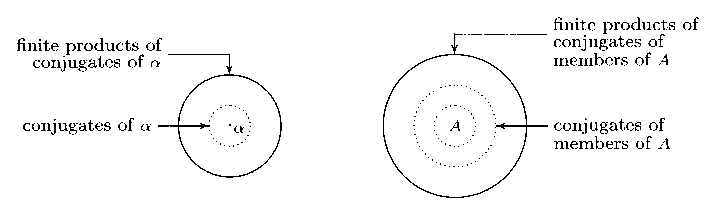
\includegraphics{chap07-vend-scan-02.eps}
\end{figure}

We demand that the polygon $P_{0}$ satisfy conditions 1)--3) of 1A, 5), and a modified form of 4):

4$^{\prime}$) The boundary of $P_{0}$ shall meet $\mathscr{Q}$ in at most a finite number of parabolic vertices and free sides.

This assumption rules out accidental vertices of the first kind.

The foregoing developments (1A--1E) then go through. The accidental vertices of the second kind are assembled in cycles of two vertices. Thus, if $\alpha_{1}$ is an accidental vertex on $\mathscr{Q}$, there exists a side $s$ beginning or ending at $\alpha_{1}$ (Fig., p. 227). The conjugate side $s^{\prime}$ ends in an accidental vertex $\alpha_{2}$ and $(\alpha_{1},\,\alpha_{2})$ is a cycle. $P_{1}$, the image of $P_{0}$ under $T^{-1}$, is a polygon bordering $P_{0}$ along $s$ and having the free side $f_{1}^{\prime}=T^{-1}f_{1}$. $P_{0}\cup P_{1}$ covers a neighborhood $K\cap \mathscr{U}$, where $K$ is a disk about $\alpha_{1}$. We see that there are exactly two polygons with vertex at a given accidental vertex. The closures of the first generation polygons cover a neighborhood of $P_{0}$; their outer boundaries constitute a Jordan curve containing $P_{0}$ in its interior. We can now prove, exactly as before, that the $P_{i}\in\Gamma P_{0}$ are disjoint.

Secondly, a straight line cannot subtend infinitely many polygons at a common accidental vertex since there are only two such polygons that meet there. This suffices to show, as in 1E, that every point of $\mathscr{U}$ lies in a polygon $\overline{P}_{i}$. The proof is complete.

We state the result in a formal theorem.

\begin{figure}[!h]
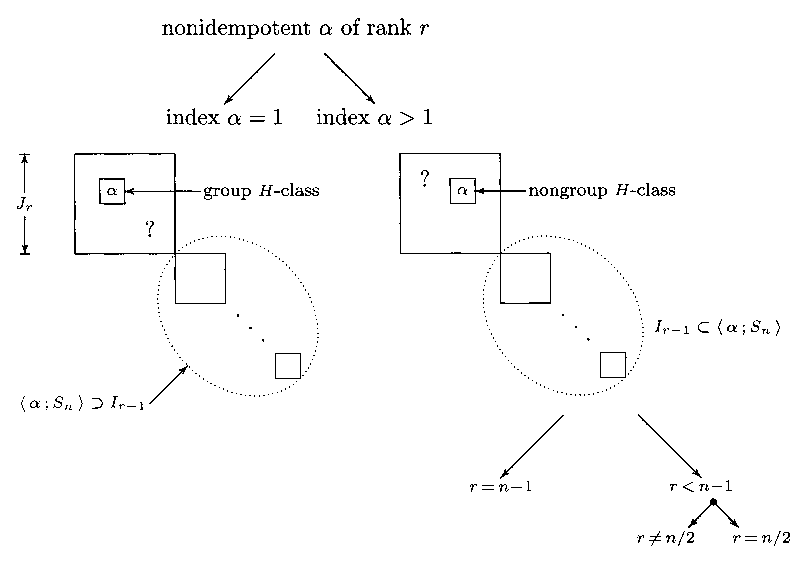
\includegraphics{chap07-vend-scan-03.eps}
\end{figure}


\begin{theorem*} [cf. note 17a, p. 403] Let $P_{0}$ be a polygon bounded by a finite number of pairs of sides $(s_{i},s_{i}^{\prime}),\,i=1,\cdots,\, n$ \emph{(}arcs of circles orthogonal to $\mathscr{Q}$\emph{)} and by at most a finite number of free sides \emph{(}arcs of $\mathscr{Q}$\emph{)}. Let $T_{i}$ be a linear transformation of $\mathscr{U}$ mapping the outside of the circle determined by $s_{i}$ on the inside of the circle determined by $s_{i}^{\prime}$. If $P_{0}$ has no free sides, let conditions \emph{1)--4)} of \emph{1A} hold; if $P_{0}$ has free sides, \emph{1)--3)} of \emph{1A} and $4^{\prime}),\, 5)$ of \emph{1F} be satisfied. Then the group $\Gamma$ generated by $\{T_{i},\,i=1,\,\cdots,\,n\}$ is a discontinuous function group with domain of existence $\mathscr{U}$ in the first case and a region containing $\mathscr{U}$ in the second case, and $P_{0}$ is a fundamental region for $\Gamma$ relative to $\mathscr{U}$.
\end{theorem*}

\subsection{}\label{ch07:sec1G}
As an example of the application of this theorem, we shall develop a subclass of the \emph{triangle groups of H. A. Schwarz}\index{triangle group}\index{Schwarz}. Let $l_{1},\,l_{2},\,l_{s}$ be integers satisfying
\begin{equation*}
\tag{$^{\ast}$} \frac{1}{l_{1}}+\frac{1}{l_{2}}+\frac{1}{l_{3}}<1,\qquad 2\leqq l_{i}\leqq\infty
\end{equation*}
with the understanding that $1/\infty=0$. Construct a noneuclidean triangle with one vertex at the origin having angles $\pi/l_{1},\,\pi/l_{2},\,\pi/l_{3}$; this is possible in view of $(^{\ast})$. Reflect this triangle in one of the sides issuing from the origin (cf. Figure). Then $OA$ is noneuclidean congruent to $OC$ and $AB$ to $BC$. Hence there is a conformal homeomorphism $T_{1}$ of $\mathscr{U}$ mapping $OA$ on $OC$ and a $T_{2}$ mapping $AB$ on $AC$. Consider the polygon $OABC$. The cycles are evidently $\{O\},\,\{AC\}$, and $\{B\}$. If all $l_{i}$ are finite these are elliptic cycles of angle sum $2\pi/l_{1},\,2\pi/l_{2}$, and $2\pi/l_{s}$, respectively. If $l_{i}=\infty$ for some $i$, that cycle is parabolic. The hypotheses of Theorem 1E are satisfied for the polygon in question and we conclude that the group generated by $\{T_{1},\,T_{2}\}$ is discontinuous and has this polygon as a fundamental region. The group is called a triangle group.

In Chapter~\ref{ch01:chap01}, p. 15 is shown the tessellation of the unit disk by fundamental regions of the triangle group for which $l_{1}=2,\,l_{2}=3,\,l_{3}=7$. Another case of interest (cf. Ch.~\ref{ch01:chap01}, p. 16) is $l_{1}=l_{2}=l_{3}=\infty$. It corresponds to the ``elliptic modular function''\index{elliptic modular function} of Jacobi\index{Jacobi}. The group is $\Gamma(2)$, the principal congruence subgroup modulo 2 of the full modular group (cf. \ref{ch03:chap03}. \ref{ch03:sec1F}, \ref{ch11:chap11}. \ref{ch11:sec3A}).

\begin{figure}[!h]
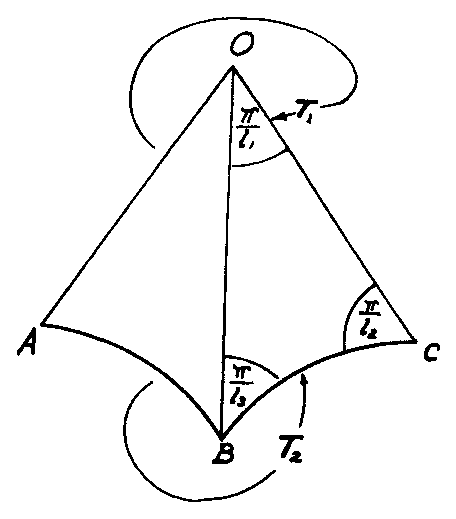
\includegraphics{chap07-vend-scan-04.eps}
\end{figure}


\subsection{}\label{ch07:sec1H}
We shall now describe one arithmetical method\index{construction of principal-circle group!by arithmetical method} for generating discontinuous groups. Such methods rely on the theorem (\ref{ch03:chap03}. \ref{ch03:sec3I}) that discreteness and discontinuity are equivalent in groups\index{group of Picard} that preserve a disk or half-plane. In looking for discrete groups we naturally encounter number theory.

Consider the group $\Gamma^{(1)}$ of matrices $(\alpha\bar{\gamma}|\gamma\bar{\alpha}),\, \alpha\bar{\alpha}-\gamma\bar{\gamma}=1$, where $\alpha,\,\gamma$ are Gaussian integers ($=a+bi, a,\,b$ being rational integers). $\Gamma^{(1)}$ is a subgroup of Picard's group (the group of all unimodular matrices with Gaussian integers for entries). Let $w =w_{1}/w_{2}$; the homogeneous group consists of transformations
\begin{align*}
w_{1}^{\prime}&=\alpha w_{1}+\bar{\gamma}w_{2},\\
w_{2}^{\prime}&=\gamma w_{1}+\bar{\alpha}w_{2}.
\end{align*}
If $T$ belongs to the homogeneous group, $T$ preserves the Hermitian form $|w_{1}|^{2}-|w_{2}|^{2}$. That is, $|w_{1}^{\prime}|^{2}-|w_{2}^{\prime}|^{2}=|w_{1}|^{2}-|w_{2}|^{2}$, as is immediately verified.

Let $\Gamma^{(n)}$ be the subgroup of the homogeneous Picard's group that leaves invariant the form
\begin{equation*}
|w_{1}|^{2}-n|w_{2}|^{2},
\end{equation*}
where the positive integer $n$ is not a perfect square. It is clear that each element of $\Gamma^{(n)}$ maps the interior of the circle $w\bar{w}=n$ on itself. Furthermore, $\Gamma^{(n)}$ is obviously discrete, hence discontinuous, in the interior of this circle.

It is not hard to see that the group $\Gamma^{(n)}$ consists of all matrices $(\alpha,\, n\bar{\gamma}|\gamma,\bar{\alpha})$, $\alpha\bar{\alpha}-n\gamma\bar{\gamma}=1$, with Gaussian integers $\alpha,\,\gamma$. $\Gamma^{(n)}$ is an infinite group. Indeed, let ($x,\, y)$ be a solution of the Pell equation (\citeauthor{Hardy0000b}\index{Hardy-Wright} [\ref{Hardy1a}, p. 210])
\begin{equation*}
x^{2}-ny^{2}=1,\qquad y\neq 0.
\end{equation*}
Obviously $|x|>1$. The matrix
\begin{equation*}
\left(\begin{matrix}x&-niy\\
iy&x\end{matrix}\right)
\end{equation*}
belongs to $\Gamma^{(n)}$ and is hyperbolic. Its powers are all distinct.

The group contains parabolic elements if and only if $n$ is the sum of two squares. For if $n=a^{2}+b^{2}$, the matrix
\begin{equation*}
\left(\begin{matrix}
1+ni&n(a-bi)\\a+bi&1-ni\end{matrix}\right)
\end{equation*}
is parabolic and belongs to $\Gamma^{(n)}$. Conversely, if $\Gamma^{(n)}$ contains a parabolic element $(\alpha, n\bar{\gamma}|\gamma,\bar{\alpha})$ we must have $\alpha_{1}=\pm 1$, where $\alpha=\alpha 1 +i\alpha_{2},\,\gamma=\gamma_{1}+i\gamma_{2}$; hence $\alpha_{2}^{2}-n(\gamma_{1}^{2}+\gamma_{2}^{2})=0$. It is a theorem that an integer $k$ is the sum of two squares if and only if every prime $p\equiv 3\ (\mathrm{mod}\,4)$ dividing $k$ divides it to an even power (\citeauthor{Hardy0000b} [\ref{Hardy1a}, p. 299]). Let $p$ be a prime congruent to 3 mod 4. Then $p$ divides $\gamma_{1}^{2}+\gamma_{2}^{2}$ to an even power and so from the above equation divides $n$ to an even power. Hence $n$ is the sum of two squares.

Quadratic forms in more variables\index{relations in a group|)} can be used to construct discrete groups. Cf. [\citeauthor{Poincare0000}~\ref{Poincare1}, pp. 64--66, pp. 463--511]. Cf. also [\citeauthor{Fricke0000a}\index{Fricke-Klein} \ref{Fricke1a}, pp. 448--584]. Groups constructed from the elements of an algebraic number field are discussed in the latter reference, pp. 585--634.

\section{The Relations in $\Gamma$}\index{relations in a group}\label{ch07:sec2}

Let $\Gamma$ be a function group with domain of existence $\mathscr{D}$ and let $R_{0}$ be its standard fundamental region (cf. \ref{ch04:chap04}. \ref{ch04:sec5A}). Here $R_{0}$ may have an infinite number of sides. We have seen that the transformations of $\Gamma$ which pair the conjugate sides of $R_{0}$ form a set of generators of $\Gamma$. In this Section we shall give a method for determining all relations among the generators. The notions of a relation and of a basis of relations were discussed in \ref{ch02:chap02}. \ref{ch02:sec5C}, to which the reader is referred for definitions and notation.

We have already observed (\ref{ch04:chap04}. \ref{ch04:sec5E}) that a ``loop'' around an ordinary vertex of $R_{0}$ gives rise to a relation. Poincar\'{e}\index{Poincar\'{e}} showed for principal-circle groups that the relations obtained in this way from a complete set of inequivalent ordinary vertices constitute a basis for the relations in $\Gamma$. We prove Poincar\'{e}'s theorem if: $\Gamma$ is a function group, $\mathscr{D}$ is a simply connected region preserved by $\Gamma$, and $R_{0}$ is a connected fundamental region of $\Gamma$ relative to $\mathscr{D}$. Note that $\mathscr{D}$ does not have to be maximal (of. \ref{ch03:chap03}. \ref{ch03:sec5C}). Thus the result is valid for the fundamental region of a group of the second kind relative to $\mathscr{U}$. Cf. Note 18, p. 403.


\subsection{}\label{ch07:sec2A}
We suppose $\mathscr{D}$ is a simply connected region preserved by each element of $\Gamma$, and $R_{0}$ is a connected fundamental region for $\Gamma$ relative to $\mathscr{D}$. We define $\mathfrak{T}$ as in (1): it is the set of elements of $\Gamma$, together with their inverses, that conjugate sides of $R_{0}$.

Let $\mathbf{R}=1$ be a relation in $\Gamma$. That is,
\begin{equation}
\label{ch07:eqn2}\mathbf{R}=S_{1}S_{2}\cdots S_{m},\qquad S_{i}\in \mathfrak{T}
\end{equation}
where $S_{i}\neq S_{i+1}^{-1}$. By $\mathbf{R}^{-1}$ we mean the word $S_{m}^{-1}\cdots S_{1}^{-1}$. We recall that $\mathbf{R}$ is said to be a consequence of (equivalent to) the relations $\mathbf{R}_{1},\,\cdots,\,\mathbf{R}_{k}$ if and only if there are $U_{j}\in\Gamma$ such that
\begin{equation*}
\mathbf{R}=\prod_{j=1}^{k}U_{j}\mathbf{R}_{j} U_{j}^{-1},\qquad 1\leqq i_{j}\leqq k,\,\epsilon_{j}=\pm 1.
\end{equation*}


\subsection{}\label{ch07:sec2B}
In order to prove the result we have in mind, it is convenient\index{congruence subgroup} to define \emph{chains, circuits}\index{chain}\index{circuit}, and \emph{loops}\index{loop}. Denote by $R_{i},\,i=0, 1, 2,\cdots$, the images of $R_{0}$ by the elements of $\Gamma$. Two regions $R_{i}$ and $R_{j}$ are called \emph{full neighbors} provided they have exactly one side in common. An ordered set of regions $R_{i_{1}},\,R_{i_{2}},\,\cdots,\,R_{i_{t}},\, i_{j}\geqq 0$, is said to be a \emph{chain} if each region is a full neighbor of its successor.

The chain $\{R_{i_{1}},\,\cdots,\,R_{i_{1}}\}$ is denoted by the symbol
\begin{equation*}
K=[i_{1},\cdots,i_{t}];
\end{equation*}
we may regard this also as an ordered set of integers. The integers $i_{j},\,i_{j+1}$ are said to be \emph{adjacent}; $i_{1}$ is called the \emph{beginning} of $K,\,i_{t}$ its \emph{end}. The chain inverse to $K$ is the chain $K^{-1}=[i_{t},\,i_{t-1},\,\cdots,\,i_{1}]$; the empty chain is the chain that contains no integers. Two chains $K_{1}=[i_{1},\,\cdots,\,i_{s}],\,K_{2}= [i_{s},\,\cdots,\,i_{t}]$ may be multiplied if the end of the first is equal to the beginning of the second:
\begin{equation*}
K_{1}K_{2}=[i_{1},\cdots i_{s},\,i_{s},\cdots i_{t}]=[i_{1}\cdots i_{s-1}i_{s}i_{s+1}\cdots\,i_{t}];
\end{equation*}
we agree to replace $\cdots i_{s}i_{s}\cdots$ by $\cdots i_{s}\cdots$ in this and similar cases.

If the beginning and end of a chain are the same integer, the chain is called a \emph{circuit}:
\begin{equation*}
[i_{1},\,\cdots,\,i_{t}=i_{1}].
\end{equation*}

A circuit may be self-intersecting: in other words $i_{j}=i_{k}$ for some $j\neq k$. We wish to decompose the circuit into ``simple circuits'' or \emph{loops}. A loop is a circuit in which no two integers are the same except the beginning and end.

First we shall partition all circuits into disjoint equivalence classes. If $C$ is a circuit and $K$ a chain, $KCK^{-1}$ is a circuit, provided $K$ and $C$ can be multiplied. We call $C$ and $KCK^{-1}$ \emph{equivalent},\index{discontinuity!and discreteness} and denote by $\{C\}$ the equivalence class containing $C$.

Now let $C=[i_{1},\,i_{2},\,\cdots,\,i_{t}=i_{1}]$ be a circuit. If $C$ is not a loop, then $i_{j}=i_{k}$ for some $j\neq k,\,1\leqq j,\,k\leqq t$. There is an $i_{m},\,m\geqq j$, and an $i_{n},\,n\leqq k$, such that $L_{1}=[i_{m}, i_{m+1},\,\cdots,\,i_{n}]$ is a loop. Define the chains
\begin{align*}
U&=[i_{1},\,i_{2},\,\cdots,\,i_{m}],\\
V&=[i_{1},\,\cdots,\,i_{m},\,i_{n+1},\,\cdots,\,i_{t}].
\end{align*}
$U$ and $L_{1}$ can be multiplied. Since $i_{m}=i_{n},\,V$ is actually a circuit. We can now write
\begin{equation*}
C=UL_{1}U^{-1}V=\tilde{L}_{1}V,
\end{equation*}
where $\tilde{L}_{1}$ is in the class $\{L_{1}\}$.

Now $V$ is a circuit of smaller length than $C$. We can apply the same process to $V$. In a finite number of steps we shall arrive at the formula
\begin{equation*}
C=\tilde{L}_{1}\tilde{L}_{2}\cdots \tilde{L}_{s},\qquad \tilde{L}_{j}\in\{L_{j}\}
\end{equation*}
where $L_{j},\,j=1,\,\cdots,\,s$ is a loop contained in the circuit $C$.


\subsection{}\label{ch07:sed2C}
Each circuit $C$ determines an equation of the form
\begin{equation*}
W(C)=1,
\end{equation*}
where $W(C)$ is a word in the generators $\mathfrak{T}$ of $\Gamma$. Of course $W(C)$ is not necessarily reduced. Let $C=[i_{1},\,\cdots,\,i_{t}=i_{1}]$. Let $V_{j}$ be the element of $\Gamma$ that maps $R_{i_{j}}$ on $R_{i_{j+1}}$. Then $V_{t-1}\cdots V_{2}V_{1}$ maps $R_{i_{1}}$ on itself and so is the identity. Now express each $V_{i}$ in the generators $\mathfrak{T}$; we then have
\begin{equation*}
\tag{$^{\ast}$} W(C)=V_{t}\cdots V_{1}=S_{1}S_{2}\cdots S_{m}=1,\qquad S_{i}\in \mathfrak{T}
\end{equation*}
as promised.

Suppose, conversely, a relation $(^{\ast})$ is given. Let $R_{0}=R_{i_{1}}$. Since $S_{1}\in \mathfrak{T}$, the region $S_{1}R_{i_{1}}=R_{i_{2}}$ is a full neighbor of $R_{i_{1}}$. The transformation $S_{1}S_{2}S_{1}^{-1}$ pairs two sides of $R_{i_{2}}$, hence $S_{1}S_{2}S_{1}^{-1}(R_{i_{2}})=S_{1}S_{2}R_{i_{1}} =R_{i_{2}}$ is a full neighbor of $R_{i_{2}}$. Finally $S_{1}S_{2}\cdots S_{m}R_{i_{1}}=R_{i_{m+1}}$ is a full neighbor of $R_{i_{m}}$. Hence $[i_{1},\,\cdots,\, i_{m+1}]$ is a chain. But $R_{i_{m+1}}=R_{i_{1}}$, since $S_{1}S_{2}\cdots S_{m}=1$, by (2). Hence $i_{m+1}=i_{1}$ and $[i_{1},\,\cdots,\,i_{m},\,i_{m+1}]$ is a circuit. We have proved:


\begin{theorem*}
Each circuit $C$ determines an equation $W(C)=1$, where $W$ is a word in the generators $\mathfrak{T}$, and conversely. If $C=K_{1}K_{2}\cdots K_{s}$, the $K_{j}$ being chains, we have
\begin{equation*}
W(C)=W(K_{s})\cdots W(K_{2})W(K_{1}).
\end{equation*}
\end{theorem*}

The final statement of the theorem is obvious. The reason for the reversal of order in the right member is that products of chains are read from left to right, whereas products of elements of $\Gamma$ are read from right to left.

\subsection{}\label{ch07:sec2D}
The last theorem reduces the problem\index{modular group in $n$ variables} in hand to the consideration of a single loop\index{loop}. Let $L=[i_{1},\,\cdots,\, i_{t}=i_{1}]$ be a loop. Choose a point in each fundamental region $R_{i_{1}},\,j=1,\cdots,\,t-1$, and connect these points by polygonal paths such that no path crosses itself or another path, and the path joining two fundamental regions remains within those regions. There results a Jordan curve composed of a finite number of line segments, and we can choose the points so that no segment passes through a vertex of a fundamental region. We also call this new polygon $L$.

$L$ bounds a region lying entirely in $\mathscr{D}$. Subdivide this region by a square grating so chosen that no square contains more than one vertex of a fundamental region $R_{i}$ and no vertex lies on a line of the grating. The grating consists of \emph{pieces}, either squares lying in the interior of $L$, or irregular shaped polygons abutting on $L$. The number of pieces is finite.\footnote{If $\mathscr{D}$ is unbounded, we must consider a grating on the complex sphere. One of the pieces will contain $\infty$.}

Now orient the grating coherently (\ref{ch02:chap02}. \ref{ch02:sec2K}). Call the oriented pieces $L_{1},\,L_{2},\cdots,L_{n}$. Each oriented piece determines a loop.


\begin{theorem*}
$W(L)=W(\tilde{L}_{n})\cdots W(\tilde{L}_{2})W(\tilde{L}_{1})$, where $L_{j}$ is a loop starting at any vertex of the $j$\emph{th} piece and
\begin{equation*}
\tilde{L}_{j}\in\{L_{j}\},\,j=1,\,\cdots,\,n.
\end{equation*}
\end{theorem*}

Note that if $L_{i}$ does not enclose a vertex, either $W(L_{i})=1$ (if $L_{i}$ lies within one fundamental region) or $W(L_{i})=VV^{-1}$ for some $V\in\Gamma$ (if $L_{n}$ intersects two neighboring fundamental regions). In the latter case we have $W(L_{i})=S_{1}\cdots\, S_{m}S_{m}^{1}\cdots S_{1}^{-1},\,S_{i}\in \mathfrak{T}$, and $W(L_{i})$ reduces to 1.

We shall prove this theorem by induction on $n$; it is trivially true for $n=1$. Suppose it is true for every subdivision of an arbitrary loop into $n-1$ pieces. Let $L$ be an arbitrary loop subdivided into $n$ pieces.

Suppose $L$ begins at $P$ (cf. Figure). Call $L_{n}$ one of the pieces of the subdivision that begins at $P$. Let $K$ be the chain common to $L_{n}$ and $L$, and $K^{\prime}$ the chain such that $L_{n}=K^{\prime}K$. Write $L=L^{\ast}K$. Then
\begin{equation*}
L^{\prime}=L^{\ast}K^{-1}
\end{equation*}
is a loop beginning at $P$ that is subdivided coherently into $n-1$ pieces, $L_{1},\,\cdots,\,L_{n-1}$. Hence
\begin{equation*}
\tag{$^{\ast}$} W(L^{\prime})=W(\tilde{L}_{n-1})\cdots W(\tilde{L}_{1}).
\end{equation*}

Now $L^{\prime}L_{n}$ is a circuit, and by Theorem 2C,
\begin{align*}
W(L^{\prime}L_{n})&=W(L_{n})W(L^{\prime})\\
&=W(K) W(K^{\prime})\cdot W(K^{\prime_{-1}}) W(L^{\ast})\\
&=W(K) W(L^{\ast})\\
&=W(L),
\end{align*}

\begin{figure}[!h]
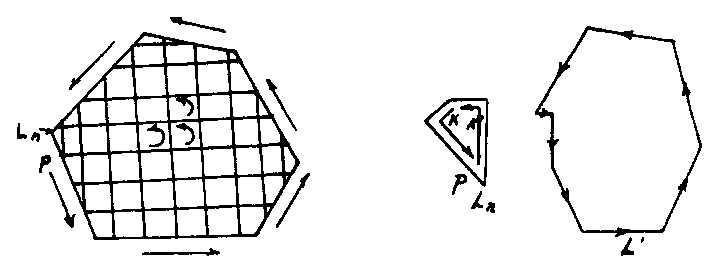
\includegraphics{chap07-vend-scan-05.eps}
\end{figure}

\noindent since obviously $W(K^{\prime})W(K^{\prime_{-1}})=1$. The theorem follows on application of $(^{\ast})$ to $W(L_{n})W(L^{\prime})$.

\subsection{}\label{ch07:sec2E}
We are now ready to prove that every relation in $\Gamma$ (cf. (1)) is a consequence of relations determined by loops around inequivalent vertices of a fundamental region. Let $\mathbf{R}=1$ be a relation. Since $\mathbf{R}$ is a word in the generators $\mathfrak{T}$ of $\Gamma$, Theorem 2C tells us that $\mathbf{R}$ determines a circuit $C$. By 2B we have $C=\tilde{L}_{1}\cdots \tilde{L}_{s}$, with $\tilde{L}_{j}\in\{L_{j}\},L_{j}$ being a loop contained in $C$. Now applying the last statement of Theorem 2C, we get
\begin{align} \label{ch07:eqn3}
\mathbf{R}&=W(C)\\
\nonumber &=W(\tilde{L}_{s})\cdots W(\tilde{L}_{2}) W(\tilde{L}_{1}).
\end{align}

Consider $W(\tilde{L}_{1})$. We have $\tilde{L}_{1}=KL_{1}K^{-1}$, with $L_{1}$ a loop. If $L_{1}$ does not contain a vertex, $W(\tilde{L}_{1})$, when reduced, equals 1 (cf. paragraph after Th. \ref{ch07:sec2D}). If $L_{1}$ does contain a vertex, $W(\tilde{L}_{1})=UW(L_{1}) U^{-1}$, where $U$ is a word in $\mathfrak{T}$. Now $W(L_{1})$, when reduced, is the left member of a \emph{relation} that we shall call $\mathbf{R}_{1}=1$. Hence, by (3),
\begin{equation*}
\mathbf{R}=U_{k}\mathbf{R}_{k}U_{k}^{-1}U_{k-1}\mathbf{R}_{k-1}U_{k-1}^{-1}\cdots U_{1}\mathbf{R}_{1}U_{1}^{-1},\qquad U_{i}\in\Gamma
\end{equation*}
where $\mathbf{R}_{1},\,\cdots,\,\mathbf{R}_{k}$ are the relations determined by loops around those vertices lying in the interior of $C$.

It remains only to show that two vertices that are equivalent under $\Gamma$ determine equivalent relations. Suppose $S\in\Gamma$ maps the first vertex, $\alpha_{1}$, on the second, $\alpha_{2}$. If the loop around $\alpha_{1}$ is $[i_{1},i_{2},\,\cdots,\,i_{t},i_{1}]$, the fundamental regions meeting at the vertex are, in order, $R_{i_{1}},\,\cdots,\,R_{i_{t}}$. Let $V_{j}$ map $R_{i_{j}}$ on $R_{i_{j+1}}$. The fundamental regions meeting at $\alpha_{2}$, are $SR_{i_{1}},\,\cdots,\,SR_{i_{1}}$, and the element of $\Gamma$ mapping $SR_{i_{j}}$ on $SR_{i_{j+1}}$ is $SV_{j}S^{-1}$. It is now clear that $S\mathbf{R}S^{-1} =1$ is the relation for $\alpha_{2}$ if $\mathbf{R}=1$ is the relation for $\alpha_{1}$.


\begin{theorem*}
Let $\mathbf{R}_{1}=1,\,\mathbf{R}_{2}=1,\cdots$ be the relations determined by loops around a full set of inequivalent ordinary vertices of a fundamental region of $\Gamma$, it being understood each loop contains exactly one vertex. Then any relation in $\Gamma$ is a consequence of a finite subset of $\{\mathbf{R}_{1},\,\mathbf{R}_{2},\,\cdots\}$. More precisely, a relation $\mathbf{R}=1$ is a consequence of exactly those $\mathbf{R}_{i}$ that  correspond to inequivalent vertices enclosed by the circuit determined by $\mathbf{R}$.
\end{theorem*}

\subsection{}\label{ch07:sec2F}
Finally we must show the relations\index{relations in a group!basis for} $\mathbf{R}_{i},\,i=1,2,\,\cdots$, are independent. In contradiction, suppose, for example, $\mathbf{R}_{1}$ is dependent on $\mathbf{R}_{2},\,\cdots,\,\mathbf{R}_{k}$. This means there are elements $V_{i}\in\Gamma$ such that
\begin{equation*}
\tag{$^{\ast}$} \mathbf{R}_{1}=V_{2}\mathbf{R}{{2}^{\varepsilon_{2}}V_{2}^{-1}}\cdots V_{k}\mathbf{R}{_{k}^{s_{k}}} V{_{k}^{-1}},\qquad \varepsilon_{i}=\pm 1.
\end{equation*}
That is, the right member, when expressed as a word in $\mathfrak{T}$, is the \emph{same word} as the left member. Let $\mathbf{R}_{i}$ be obtained by a loop around the vertex $\alpha_{i},\,i=1, 2,\cdots$. If we start at a point in a given fundamental region and construct the polygon determined by the right member of $(^{\ast})$, we obtain a circuit enclosing the vertices $V_{2}\alpha_{2},\,\cdots,\, V_{k}\alpha_{k}$ \emph{and no others}. For by the theorem just proved, every vertex enclosed by a circuit must figure in the relation determined by that circuit. It is now clear that an equation of the form $(^{\ast})$ is impossible. For since the two members are the same words in $\mathfrak{T}$, they determine the same circuits, but one of these circuits encloses $\alpha_{1}$ while the other does not. This concludes the proof of our main result:


\begin{theorem*}
Let $\Gamma$ be a\index{subgroup of discontinuous group!genus of|)} function group,\index{subgroup of discontinuous group!existence of \_\_\_s of given index|)} $\mathscr{D}$ a simply connected region preserved by $\Gamma$, and $R_{0}$ a connected fundamental region for $\Gamma$ relative to $\mathscr{D}$. Denote by $\{\alpha_{i},\,i=1,2,\,\cdots\}$ a complete set of inequivalent ordinary vertices of $R_{0}$ and by $\mathbf{R}_{i}=1$ the relation determined by $\alpha_{i}$. Then
\begin{equation*}
\mathbf{R}_{1}=1,\qquad \mathbf{R}_{2}=1,\cdots
\end{equation*}
is a basis for the relations in $\Gamma$.
\end{theorem*}

\section{Construction of Principal-Circle Groups of Given Signature}\index{congruence subgroup|)}\index{power series in $n$ variables!signature}\label{ch07:sec3}

A principal-circle group $\Gamma$ has certain characteristics that are the same in each fundamental region, in particular: the genus $g$, the number $n$ of inequivalent fixed points\footnote{By ``fixed point'' we mean always elliptic or parabolic fixed point.} $\alpha_{1},\,\cdots,\, \alpha_{n}$, and the order $l_{i}$ of the generator of the subgroup\footnote{$\Gamma_{\alpha}$ is the subgroup of $\Gamma$ consisting of those elements that fix the point $\alpha$.} $\Gamma_{\alpha_{i}}$. (We write $l_{i}=\infty$ if the generator is parabolic.) We call the symbol
\begin{equation}\label{ch07:eqn4}
\begin{array}{ll}
& g\geqq 0,\\
(g, n;l_{1},\,l_{2},\,\cdots,\,l_{n}),& n\geqq 0,\\
&2\leqq l_{i}\leqq\infty
\end{array}
\end{equation}
the \emph{signature} of $\Gamma$. Every principal-circle group with a finite number of sides has a signature; we can read the signature directly from the fundamental region. The constants $l_{i}$ can be determined by applying the result of the last Section.

The object of this Section is to prove the converse: every signature (4) with one exception is the signature of a principal-circle group. To do this we have only to construct a hyperbolic polygon in $\mathscr{U}$ having certain angles and sides. The result will then follow from the theorems of Sections~\ref{ch07:sec1} and \ref{ch07:sec2}.

It should be kept in mind that there are uncountably many groups having the same signature, if we exclude certain signatures of genus $0$ or 1. This is true even if we do not distinguish between groups that are conjugate to each other by a homeomorphism of $\mathscr{U}$.

\subsection{}\label{ch07:sec3A}
Let the signature (4) be given. In $\mathscr{U}$ draw a regular euclidean polygon of $4g+n$ sides inscribed in a circle with center at the origin $O$ and radius $r,\,0<r<1$. Now replace each side by the hyperbolic arc connecting its endpoints.

Let $H_{i}H_{i+1}$ be the curved\index{power series in $n$ variables!relations in a} side labelled $4g+i,\,i=1,\,\cdots,\,n$, and let $M_{i}$ be its midpoint; $H_{n+1}$ coincides with the initial point of side 1 (Fig., p. 236). The interior angle subtended by $H_{i}H_{i+1}$ at $M_{i}$ is $\pi$. Since the angle $H_{i}K_{i}H_{i+1}$ is $0,\, K_{i}$ being the point where the radius through $OM_{i}$ cuts the circle $\mathscr{Q}$, we can find a point $N_{i}$ on $OM_{i}K_{i}$ such that the interior angle $H_{i}N_{i}H_{i+1}$ is $2\pi/l_{i}$. (If $l_{i}=\infty,\, N_{i}$ is on $\mathscr{Q}.)$ We construct the new sides $H_{i}N_{i}H_{i+1}\,(1\leqq i\leqq n)$ and now have a $(4g+2n)$-sided polygon. This polygon depends on the value of $r$ selected and so will be denoted by $P_{r}$.

According to our construction the angles $H_{i}N_{i}H_{i+1}$ do not change as we vary $r$ from 0 to 1. Let $\tau(r)$ be the sum of the angles of $P_{r}$ other than $\{H_{i}N_{i}H_{i+1}\}$. As $r$ changes, $\tau$ changes for two reasons: the homothetic variation of $P_{r}$, and the alteration in the angles contributing to $\tau$ by keeping each of the angles $H_{i}N_{i}H_{i+1}$ at its value $2\pi/l_{i}$. Since both processes are continuous, it is clear that $\tau(r)$ varies continuously with $r$.

Now assume
\begin{equation} \label{ch07:eqn5}
K=2g-2+\sum\limits_{i=1}^{n}(1-l_{\ \ i}^{-1})>0.
\end{equation}
Let $\sigma=\sum\nolimits_{i=1}^{n}l_{i}^{-1}$. As $r \rightarrow 1$, the vertices of $P_{r}$ other than $\{N_{i}\}$ tend to $\mathscr{Q}$; hence $\tau(r)\rightarrow 0$. As $r\rightarrow 0,\,P_{r}$ approaches a euclidean polygon of $4g+2n$ sides, hence $\tau(r)\rightarrow(4g +2n-2)\pi-2\pi\sigma$, which is equal to $2\pi(K+1)$. Since $K>0$, this gives $\tau(0)>2\pi$. It follows that there is an $r_{0},\,0<r_{0}<1$, for which $\tau(r_{0})=2\pi$. The polygon $P_{r_{0}}$ we shall call simply $P_{0}$.

\begin{figure}[!h]
\includegraphics{chap07-vend-scan-06.eps}
\end{figure}

We can set up linear transformations of $\mathscr{U}$ pairing the sides of $P_{0}$. Select $g$ transformations $A_{1},\,\cdots,\,A_{g}$ so that $A_{1}$ pairs the sides (1, 3), $A_{2}$ the sides $(5, 7),\cdots,$ and $A_{g}$ the sides $(4g -3,\,4g-1)$; this is possible since the paired sides are of equal noneuclidean length. Next, choose $B_{1},\,\cdots,\,B_{g}$, so that $B_{1}$ pairs the sides $(2,\,4),\,\cdots,\,B_{g}$ the sides $(4g-2,4g)$. Finally, construct substitutions $U_{i},\,i=1,\,\cdots,\,n$, which conjugate the sides $H_{i}N_{i},\,N_{i}H_{i+1}$ (cf. Figure). $U_{i}$ will be elliptic $(=E_{j})$ if $N_{i}\in\mathscr{U}$; it will be parabolic $(=P_{k})$ if $N_{i}$ is on $\mathscr{Q}$. Then $N_{i}$ is an elliptic or parabolic cycle of one vertex.

The polygon $P_{0}$ satisfies the conditions of Theorem 1F; hence, it defines a discontinuous principal-circle group $\Gamma$ of signature (4). By Theorem 2F tho independent relations of $\Gamma$ can be determined from small loops drawn around the vertices; they are
\begin{equation}\label{ch07:eqn6}
\begin{split}
&E_{i^{i}}^{l}=1,\qquad i=1,2,\,\cdots,\,s\\
P_{1}P_{2}\cdots P_{n-s}E_{1}&E_{2}\cdots E_{s}A_{1}B_{1}A_{1}^{-1}B_{1}^{-1}\cdots A_{g}B_{g}A_{g}^{-1}B_{g}^{-1}=1,
\end{split}
\end{equation}
if there are $s$ elliptic vertices and $n-s$ parabolic vertices arranged cyclically in the order given by the second line. It is easier, however, to examine the Figure on p. 238 directly and apply the process for finding the remaining vertices of the cycle determined by $H_{1}$ (\ref{ch04:chap04}. \ref{ch04:sec4G}). The relation which results (\ref{ch04:chap04}. \ref{ch04:sec5E}) is seen to be the one in the second line of (6) (for the case pictured in the Figure). The relations in the first line follow at once from the existence of the cycles $\{N_{1}\},\,\{N_{2}\}$. Although we have used the Figure, the reasoning is general.

We have therefore achieved our aim provided the condition (5) is satisfied. The group $\Gamma$ is \emph{horocyclic}.


\subsection{}\label{ch07:sec3B}
But the condition (5) is also \emph{necessary}\index{cycles!accidental, and fixed point cycles} for the existence of a horocyclic group. On p. 404 (Note 19) it is proved that all normal polygons of a given group have the same hyperbolic area: We can therefore use the particular normal polygon $P_{0}$ constructed in 3A. Draw straight lines from $0$ to each vertex of $P_{0}$, dividing it into $4g+2n$ hyperbolic triangles. Using the Gauss-Bonnet formula (p. 185, Ex. 1) we find the area to be
\begin{equation*}
(4g\,+2n)\pi-\Big\{2\pi\,+2\pi\sum\limits_{i=1}^{n}\frac{1}{l_{i}}+2\pi\Big\}.
\end{equation*}
Hence the hyperbolic area of $P_{0}$ is just $2\pi K$. Since the area must be positive, $K$ is positive. Hence we have proved:


\begin{theorem*}
There is a horocyclic group with signature $(g,\,n;l_{1},\,\cdots,l_{n})$ if and only if

\begin{figure}[h]
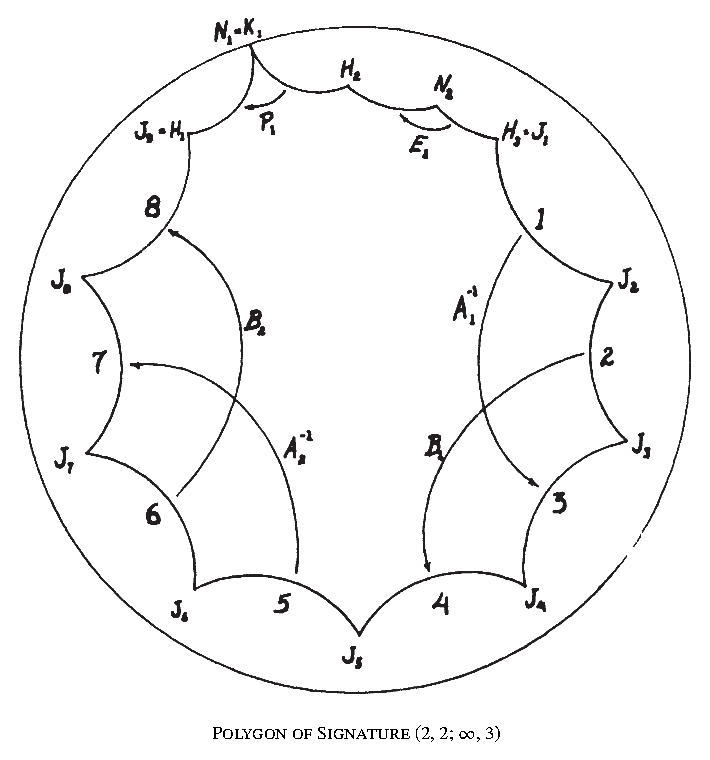
\includegraphics{chap07-vend-scan-07.eps}
\end{figure}
\setcounter{equation}{4}
\begin{equation} \label{ch07:eqn5a}
2g\,-2+\sum\limits_{i=1}^{n}(1-l_{i}^{-1})>0
\end{equation}
holds.
\end{theorem*}

\subsection{}\label{ch07:sec3C}
The remaining exceptional signatures except $(0,0)$ can be realized by principal-circle groups of the second kind. They are
\begin{align*}
&g=1,\,n=0;\\
&g=0,\,n=0,1,2;\,n=3,\,\sigma\geqq 1;\,n=4,\,\sigma\geqq 2.
\end{align*}

An elliptic or parabolic cyclic group\index{cyclic group!genus of} has genus zero. In order to see this it is advisable to triangulate the fundamental region. The Figure illustrates the case of an elliptic cyclic group. The fundamental region is bounded by the arcs $CAD$ and $CBD$, which are equivalent, and contains the point $\infty$. There are 4 inequivalent vertices $A,\,C,\,D$, and $\infty$. There are 6 inequivalent sides: $CA,\,AD$, and the lines leaving $A,\, B,\,C,\,D$; and there are 4 triangles. Hence the genus is $0$.

\begin{figure}[!h]
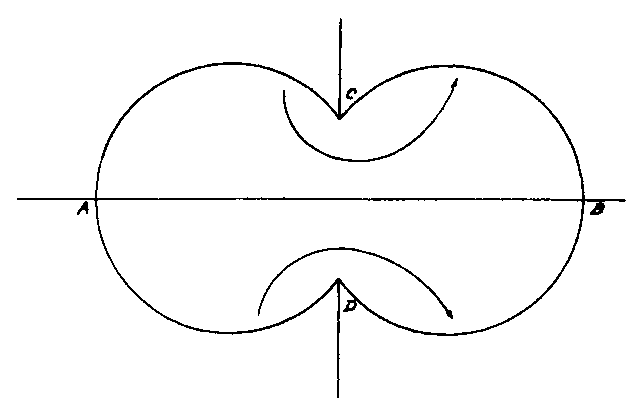
\includegraphics{chap07-vend-scan-08.eps}
\end{figure}

\begin{figure}[!h]
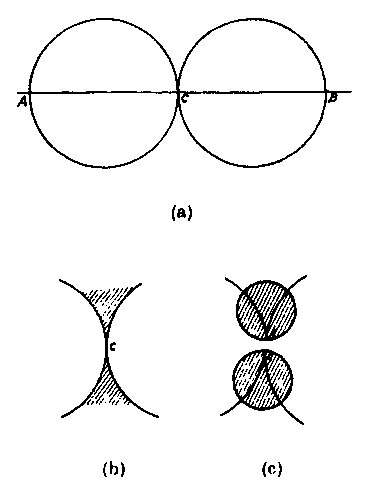
\includegraphics{chap07-vend-scan-09.eps}
\end{figure}

A parabolic cyclic group is shown in the Figure (a) above. One must be careful to count $C$ as \emph{two} vertices. Otherwise $C$ does not have a neighborhood of the type required for parabolic vertices (\ref{ch06:chap06}. \ref{ch06:sec3A}). Cf. Figures (b), (c).

A hyperbolic cyclic group, on the other hand, has genus 1 and no fixed points.

The above discussion disposes of the classes (0, 1) and (1, 0).

To treat $(0,\,2;\,l_{1},\,l_{2})$, construct a group of the second kind with the fundamental region shown in the Figure below. The triangulation shown reveals that the genus is $0$: there are 7 vertices (counting $\infty$), 17 sides, and 12 triangles. The case illustrated has $l_{1}<\infty,\, l_{2}=\infty$, but obviously all values of $l_{1}$ and $l_{2}$ can be covered.

\begin{figure}[!h]
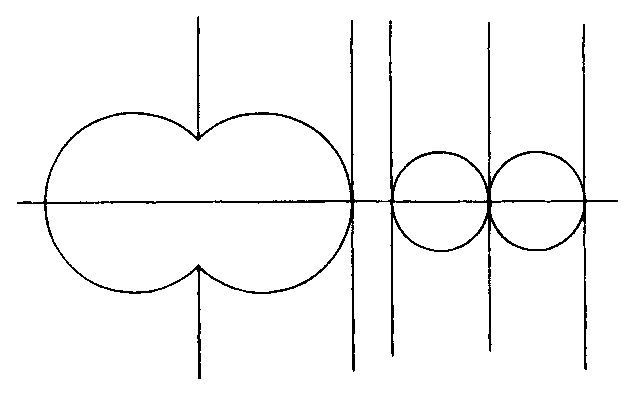
\includegraphics{chap07-vend-scan-10.eps}
\end{figure}

A similar scheme suffices for the exceptional groups in the classes (0, 3), (0, 4).

This leaves only the class (0,0). It is easy to see that there is no group with this signature. For a horocyclic group of this class Euler's formula would read $m=q+1$. Since there are no fixed points, each cycle has at least two vertices. Thus the number of vertices is at least $2m=2q+2$, which is impossible in a polygon of $2q$ sides. Suppose $\Gamma$ is of the second kind. We consider the fundamental polygon in the whole plane, i.e., we adjoin to $N$ its reflection in $\mathscr{Q}$. If the free sides on $\mathscr{Q}$ are drawn, the enlarged fundamental region is divided into two cells (one inside, one outside, $\mathscr{Q})$, and Euler's formula is applicable. Let $m,\,q$ be the number of cycles and pairs of conjugate sides in the original fundamental region $N$; write $m=m_{1}+m_{2}$, where $m_{1}$ is the number of cycles in $\mathscr{U};\,m_{2}$, the number on $\mathscr{Q}$. Then $2m_{1}+m_{2}-2q-f+2=2$. A cycle in $\mathscr{U}$ or on $\mathscr{Q}$ has at least two vertices. Thus we have at least $2m_{1}+2m_{2} =2q+f+m_{2}$ vertices in $N$. Since $m_{2}>0$ ($\Gamma$ is of the second kind), we again get a contradiction. Here $f$ is the number of free sides. To summarize:


\begin{theorem*}
Each signature in the class $(g,\,n)$, where
\begin{equation*}
g\,\geqq 0,n\geqq 0,\,g+n>0,
\end{equation*}
is the signature of a principal-circle group.
\end{theorem*}

\section{The Canonical Polygon}\index{canonical polygon}\label{ch07:sec4}

The fundamental regions constructed in Section~\ref{ch07:sec3} have certain special features. The number of sides for a group with signature $(g,\,n)$ is $4g+2n$. Each elliptic and parabolic cycle consists of a single vertex, and there is one accidental cycle. Furthermore, the order of the sides is prescribed. Such a fundamental region\index{fundamental region!of group in $n$ variables} is called a \emph{canonical polygon}.

\begin{definition*}
Let $\Gamma$ be a horocyclic group\footnote{Theorem 3B shows that the parameters $g,\,n$ are restricted by the assumption that $\Gamma$ is horocyclic.} of signature $(g,\,n)$. A fundamental region $\Pi$ is a canonical polygon provided it is a polygon bounded by $4g+2n$ analytic arcs arranged in the following cyclic order:
\begin{equation*}
a_{1}b_{1}a_{1}^{\prime} b_{1}^{\prime}a_{2}b_{2}a_{2}^{\prime}b_{2}^{\prime}\cdots a_{g}b_{g}a_{g}^{\prime}b_{g}^{\prime}h_{1}h_{1}^{\prime}h_{2}h_{2}^{\prime}\cdots h_{n}h_{n}^{\prime}.
\end{equation*}
Here the conjugate side is indicated by a prime. The intersection of $h_{j},\,h_{j}^{\prime}\,(j=1,\cdots, n)$ shall constitute a cycle of one vertex, the remaining vertices constituting a single accidental cycle.

In this Section we shall show every horocyclic group of finite signature admits a canonical polygon. We assume the principal circle is the unit circle~$\mathscr{Q}$.
\end{definition*}

\textit{Remarks.} 1) In \citeauthor{Fricke0000a}\index{Fricke-Klein} [\ref{Fricke1a}] the canonical polygon is defined as above except it is required to be a convex polygon bounded by hyperbolic arcs. The proof is highly involved; it appears on pp. 294--320 of the above reference. A new proof for $g>0$ has now been given (cf. Note 20, p. 405).

2) The theorem we are about to prove does \emph{not} imply that every finitely generated horocyclic group possesses a canonical polygon, in particular, a polygon with a finite number of sides. By assuming $\Gamma$ to have finite genus $g$ we have already assumed the Riemann surface of $\Gamma$ to be compact, and the finiteness of the number of sides then follows from \ref{ch06:chap06}. Th. \ref{ch06:sec3F}. Cf. Note 21, p. 405.

\subsection{}\label{ch07:sec4A}
By~\ref{ch04:chap04}. Theorem 7G we can select a normal polygon for $\Gamma$ having the following properties:
\begin{enumerate}
\item[1)] Each elliptic and parabolic cycle consists of a single vertex.
\item[2)] There are no ordinary cycles lying on $\mathscr{Q}$.
\end{enumerate}
Let $N$ be such a polygon. We shall show how it is possible, by adding and subtracting portions of $N$, to obtain a canonical polygon.

For this purpose we use \emph{allowable modifications}. Let the sides of $N$ be described in counterclockwise order. Suppose $a,\,a^{\prime}$ are a pair of conjugate sides. Draw an analytic arc\footnote{An analytic arc is the image of the interval $0\leqq t \leqq 1$ by an analytic function of the real variable $t$.} $f$ that connects two vertices of $N$, lies except for its endpoints entirely in $N$, and divides $N$ into two polygons $N_{1}$ and $N_{2}$, neither one containing both $a$ and $a^{\prime}$ (cf. Figure). Suppose $a\in N_{1}$ and let $Va=a^{\prime},\, V\in\Gamma$. Then $V\bar{N}_{1}$ intersects $\bar{N}_{2}$ exactly in $a^{\prime}$, and it is clear that $\mathrm{Int}\{\bar{N}_{2}\cup V\bar{N}_{1}\}$ is still a fundamental region, which is, moreover, bounded by pairs of analytic arcs. This process, illustrated in the Figure, is called an allowable modification; under it the number of sides does not change.

\begin{figure}[!h]
\includegraphics{chap07-vend-scan-11.eps}
\end{figure}

The sides of $N$ that are conjugated by an element of $\Gamma$ having a fixed point are called sides of the second class; the remaining ones, sides of the first class. Two conjugate sides of the second class are adjacent, their intersection being the fixed point. For the same reason two conjugate sides of the first class are never adjacent. Under the particular allowable modifications used below each side is mapped into a side of the same class and adjacent sides of the second class remain adjacent. For a fixed point stays fixed and an accidental vertex stays accidental.


\subsection{}\label{ch07:sec4B}
Suppose we have a sequence $\cdots a\,e\,e^{\prime}\,b\cdots$, where $e$ is of course in the second class. By an allowable modification we can replace this sequence by $\cdots f\,f^{\prime}\,a\,b\cdots$. In fact, draw the diagonal $f$ and map $e$ \emph{on} $e^{\prime}$, as shown in the Figure. Note that $f,\,f^{\prime}$ are in class two since they intersect in the fixed point $A$. Since the mapping involved is conformal, it is seen that the angle between $f$ and $f^{\prime}$ is equal to the angle between $e$ and $e^{\prime}$.

\begin{figure}[!h]
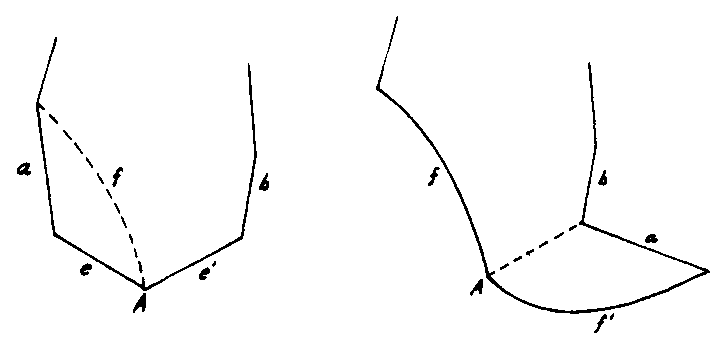
\includegraphics{chap07-vend-scan-12.eps}
\end{figure}

To treat the sequence $P_{1}ee^{\prime}P_{2}ff^{\prime}$, the $P_{i}$ being blocks containing no sides of the second class, draw a diagonal from the beginning of $P_{1}$ to the end of $e$ and map $e$ on $e^{\prime}$, getting $ee^{\prime}P_{1}P_{2}ff^{\prime}$. In finitely many steps we have a polygon $B_{2}B_{1}$, where $B_{2}$ contains all sides of the second class.


\subsection{}\label{ch07:sec4C}
We now concentrate on sides of the first class. We call two sides $a,\,b$ \emph{linked} if they and their conjugates occur in the order $\cdots a\cdots b\cdots a^{\prime}\cdots b^{\prime}\cdots$. (Only the cyclic order is important; thus the above order is the same as $\cdots b\cdots a^{\prime}\cdots b^{\prime}\cdots a\cdots$.) We assert that $B_{1}$ contains a pair of linked sides.

To prove it, notice first that $B_{1}$ contains at least 4 sides. For $N$ has an even number of sides and so has $B_{2}$, therefore also $B_{1}$. If $B_{1}$ contained only two sides, the sides would be conjugate but also adjacent.

Let the sides of $B_{1}$ be $c_{1}c_{2}\cdots$, the side $c_{1}$ (the ``first'' side of $B_{1})$ being the side immediately following $B_{2}$. Let $c_{1}\cdots c_{s}$ be the longest block in $B_{1}$ containing no two conjugate sides. Clearly $s\geqq 2$. The side $c_{s}$ is not the last side of $B_{1}$. Hence $c_{s+1}$ is in $B_{1}$ and is a conjugate of a preceding side $c_{j},j\leqq s$. Now $j\neq s$, for then $c_{s},\,c_{s+1}$ would be adjacent conjugate sides. Hence $j<s$ and it is seen that $c_{j},\, c_{j+1}$ form a linked pair. Write
\begin{equation*}
c_{j}=a,\qquad c_{j+1}=b.
\end{equation*}

We now make two allowable modifications as illustrated schematically in the Figure, where $W,\,X,\,Y,\,Z$ are blocks of sides in $B_{1}$. In the first we map $b$ on $b^{\prime}$; in the second, $a$ on $a^{\prime}$. As a result we have the sequence
\begin{equation*}
B_{2}\,Z\,X\,W\,e\,d\,e^{\prime}\, d^{\prime}Y.
\end{equation*}

\begin{figure}[!h]
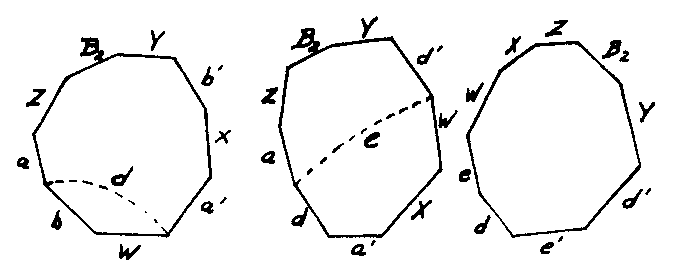
\includegraphics{chap07-vend-scan-13.eps}
\end{figure}

By using the process outlined earlier we can move $Y$ to the other side of $B_{2}$, obtaining $B_{2}\,Vede^{\prime}d^{\prime}$, with $V$ a block in $B_{1}$. As before, $V$ must contain a linked pair $c,\, d$, and by allowable modifications we can change the order of the sides to read $B_{2}Ufgf^{\prime} g^{\prime}eded^{\prime}$, with $U$ a block in $B_{1}$. In the process the sequence $ede^{\prime}d^{\prime}$ is not disturbed. After a finite number of repetitions of this procedure, $B_{1}$ will be of the form
\begin{equation*}
a_{1}b_{1}a^{\prime}_{1}b_{1}^{\prime}\cdots a_{r}b_{r}a^{\prime}_{r}b_{r}^{\prime},
\end{equation*}
as desired.


\subsection{}\label{ch07:sec4D}
The polygon $N$ has now been transformed into a polygon $\Pi$ whose sides are analytic arcs. The number of sides of the second class is evidently $2n$, since there are $n$ classes of fixed points. The sides of the first class are arranged in blocks $a_{i}b_{i}a_{i}^{\prime}b_{i}^{\prime}$ and so their number is a multiple of 4, say $4k$. It is not hard to see that the endpoints of all sides of the first class are equivalent under $\Gamma$. Moreover, if $B_{2}=h_{1}h_{1}^{\prime}\cdots h_{n}h_{n}^{\prime}$ with $h_{j}=H_{j}N_{j},\,h_{j}^{\prime}=N_{j}H_{j+1}$ (cf. Figure on p. 237), then $H_{j}$ is equivalent to $H_{j+1}$ and so all $\{H_{j},j=\,1,2,\,\cdots,\,n+1\}$ are equivalent. But $H_{n+1}=J_{1}$ and $H_{1}=J_{4k+1}$. We have then a cycle $(J_{1}, J_{2},\,\cdots,\,J_{4k},\,H_{1},\,H_{2},\,\cdots,\, H_{n})$ of $4k+n$ vertices and this cycle is accidental.

In the polygon $\Pi$, then, there are $n+1$ cycles, one accidental and $n$ fixed point cycles. From Euler's formula we get
\begin{equation*}
n+1-(n+2k)+1=2-2g,
\end{equation*}
whence
\begin{equation*}
k=g.
\end{equation*}

The polygon $\Pi$ consists of $4g+2n$ sides. These sides are arranged in conjugate pairs.

At each stage of the above process angles are preserved, both the total angle sum of the polygon and the angle of intersection of two conjugate sides meeting at a fixed point. We can use the results of IV. 4, which hold for $N$, and can say that an elliptic vertex in $\Pi$ subtends an angle of $2\pi/l$; a parabolic vertex, a zero angle. The sum of the angles at the accidental cycle of $4g+n$ vertices is $2\pi$.

This completes the proof of:


\begin{theorem*}
A horocyclic group of finite signature possesses a canonical polygon.
\end{theorem*}

\subsection{}\label{ch07:sec4E}
If $\Gamma$ is a group of the second kind, there are some free sides, say $f_{1},f_{2},\,\cdots,\,f_{r}$. In this case also there is a canonical polygon $\Pi$, and its sides appear in the following order:
\begin{equation*}
a_{1}b_{1}a_{1}^{\prime}b_{1}^{\prime}\cdots a_{g}b_{g}a_{g}^{\prime} b_{g}^{\prime}h_{1}h_{1}^{\prime}\cdots h_{n}h_{n}^{\prime}c_{1}f_{1}c_{1}^{\prime}\cdots c_{r}f_{r}c_{r}^{\prime}.
\end{equation*}
The proof is made by similar arguments and will not be given.

If $\Gamma$ is considered to act in the unit disk, the associated Riemann surface is, of course, not compact, but it is compact if $\Gamma$ acts in the whole plane. To compute the genus we ``double'' the polygon $\Pi$, i.e., adjoin to $\Pi$ its reflection in $\mathscr{Q}$. Then it is readily seen that the doubled Riemann surface has genus $2g+r-1$. We may therefore write the signature of $\Gamma$ as
\begin{equation*}
(2g+r-1,\,r,\,n;\quad l_{1},\,\cdots,\,l_{n}),\qquad g\geqq 0,\,r\geqq 1,\,n\geqq 0.
\end{equation*}
In order that a group with this signature should exist, it is necessary to place certain additional restrictions on the parameters.

By Theorem 2F the relations in $\Gamma$ are generated by
\begin{equation*}
h_{1}^{l_{1}}=\cdots=h_{s}^{l_{s}}=1,
\end{equation*}
where $h_{i}$ is an elliptic element of order $l_{i}$.


\subsection{}\label{ch07:sec4F}
The theorem of Section 4D was first proved by \citeauthor{Klein0000}\index{Klein}\index{canonical polygon!Klein's existence proof} ([\ref{Klein1}, pp. 676--678]). We give a brief outline of his proof.

Let $\sigma$ be the projection $\mathscr{U}^{+}\rightarrow S=\Gamma\backslash \mathscr{U}^{+}$. Let $e_{1},\,\cdots,\,e_{n}$ be the projections of the fixed points in $\mathscr{U}^{+}$ and let $O\in S$ be different from $\{e_{i}\}$. The surface $S$ is of genus $g$ and may be made simply connected by a system of $2g$ retrosections (cross cuts) all starting from and returning to $O$. Join $O$ to the points of $\{e_{i}\}$ by arcs that do not cut the retrosections or each other. Denote the union of the retrosections and arcs by $K$.

It is possible to define a single-valued branch $f$ of $\sigma^{-1}$ on the domain $S-K$. Then $f$ is 1-1 from $S-K$ to $\Pi=f(S-K)$. $\Pi$ is seen to be a fundamental region. The boundary of $\Pi$, namely $f(K)$, is found by tracing $K$, being careful to distinguish between the two ``banks'' of a cut. The banks of the cuts map into the sides of $\Pi$, banks of the same cut going into conjugate sides. The mapping $f$ is conformal except at the points $e_{i}$. The polygon $\Pi$ is a canonical polygon.

The process is illustrated in the Figure, drawn for $g=2,\,n=3$.

\begin{figure}[!h]
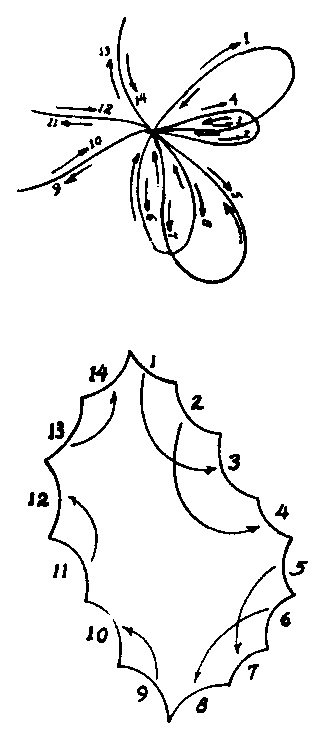
\includegraphics{chap07-vend-scan-14.eps}
\end{figure}


\section{Representations of Discontinuous Groups}\index{representation!of discontinuous group}\label{ch07:sec5}

We recall that a representation\index{Poincar\'{e} series of $n$ variables} of a group $G$ is a homomorphism of $G$ into a group of matrices $G^{\prime}$; the representation is \emph{faithful} if the homomorphism is an isomorphism (\ref{ch02:chap02}. \ref{ch02:sec5F}). If $G^{\prime}$ is simple enough, it may be possible to determine group properties by calculations with the matrices, and if the representation is faithful, these will be properties of $G$. For an example, cf. \ref{ch07:sec6D}.

In this Section we are going to develop faithful representations for a class of discontinuous groups (cf. \citeauthor{Lehner0000}~[\ref{Lehner10}])\index{Lehner}.

\subsection{}\label{ch07:sec5A}
As a first case we consider a free group\index{representation!of free group} $G$ with a countable number of generators\index{Poincar\'{e} series of $n$ variables!convergence of} $t_{1},\,t_{2},\cdots$. Corresponding to $t_{j}$ define
\begin{equation*}
T_{j}=\bigg(\begin{matrix}
-r_{j} & -1+r_{j}^{2}\\
1 & -r_{j}
\end{matrix}\bigg),
\end{equation*}
where $r_{j}$ is a rational integer and
\begin{equation*}
r_{j+1}-r_{j}\geqq 3,\qquad r_{1}\geqq 2.
\end{equation*}
The isometric circle$^{9}$\index{isometric circle} of $T_{j}$ is $|z-r_{j}|=1$, that of $T_{j}^{-1}$ is $|z+r_{j}|=1$. The set of isometric disks $\{\mathscr{R}(T_{j}),\,\mathscr{R}(T_{j}^{-1}),j=1,\,2,\,\cdots\}$ is pairwise disjoint because of the restrictions placed on $r_{j}$.

\setcounter{footnote}{8}
Denote by $G^{\ast}$ the group generated by $\{T_{1},\,T_{2},\,\cdots\}$. Clearly $G^{\ast}$ is a subgroup of the modular group. Let $S_{k}S_{k-1}\cdots S_{1}$ be a word in $G^{\ast}$. Each $S_{i}$ is a $T_{j}$. It may happen that $S_{i+1}=S_{i}$, but we never have $S_{i+1}=S_{i}^{-1}$. Suppose $P$ lies outside every isometric disk $\mathscr{R}(T_{j}),\,\mathscr{R} (T_{j}^{-1}),\,j=1,2,\, \cdots$. Then\footnote{Cf. \ref{ch02:chap02}. \ref{ch02:sec10A}.} $S_{1}(P)$ lies inside $\mathscr{R} (S_{1}^{-1})$. Since $S_{1}(P)$ lies outside $\mathscr{R}(S_{2})$---this is true even if $S_{2}=S_{1}$---it is seen that $S_{2}S_{1}(P)$ is inside $\mathscr{R}(S_{2}^{-1})$. We conclude $Q=S_{k}\cdots S_{1}(P)$ is inside $\mathscr{R}(S_{k}^{-1})$ and so is not equal to $P$. Hence $S_{k}\cdots S_{1}\neq I$. This shows that $G^{\ast}$ is a free group. Since $G$ and $G^{\ast}$ are free groups with the same cardinal number of generators, they are isomorphic. We have proved:


\begin{theorem*}
Every countably generated free group is faithfully represented by a subgroup of the modular group.
\end{theorem*}

Because of the arbitrariness of the $\{r_{j}\}$, the above construction yields infinitely many inequivalent representations.

\subsection{}\label{ch07:sec5B}
Next we consider groups with relations. Suppose $G$ is countably generated by $t_{1},\,t_{2},\cdots$ and has defining relations
\begin{equation*}
\tag{$^{\ast}$} t_{1}^{q_{1}}=t^{q_{2}}_{2}=\cdots =t_{n}^{q_{n}},=1,\qquad q_{j} = \mathrm{integer} \geqq 2.
\end{equation*}
To $t_{j}$ we make correspond
\begin{align*}
T_{j}&=\bigg(\begin{matrix}
p_{j} & p_{j}(\lambda_{j}-p_{j})-1\\
1 & \lambda_{j}-p_{j} &
\end{matrix}\bigg),\qquad j=1,2,\,\cdots,\,n\\
T_{j}&=\bigg(\begin{array}{lc}
-r_{j} & -1 + r^{2}_{j}\\
1 & -r_{j}\end{array}\bigg),\qquad j=n+1,\,n+2,\cdots
\end{align*}
where
\begin{equation*}
\lambda_{j}=2\cos\pi/q_{j},
\end{equation*}

and $p_{j},\,r_{j}$ are rational integers subject to the conditions
\begin{align*}
&p_{j+1}-p_{j}>2+\lambda_{j+1},\qquad j=1,\,\cdots,\,n\\
&\ r_{j+1}-r_{j}\geqq3,\quad j=n+1,\, n+2,\cdots;\\
&r_{n+1}\geqq 3\,+p_{n},\quad -r_{n+1}\leqq p_{1}-\lambda_{1}-3.
\end{align*}
The effect of these inequalities is to make the isometric disks $\{\mathscr{R}(T_{j}),\,\mathscr{R}(T_{j}^{-1}),j>n\}$ disjoint from\index{Poincar\'{e} series of $n$ variables!as automorphic form} each other and from the disks $\{\mathscr{R}(T_{j}), \mathscr{R}(T_{j^{-1}}),\,1\leqq j\leqq n\}$. The latter form intersecting pairs for each value of $j$, but each pair is disjoint from the other pairs. In case $q_{j}=2$, however, $\mathscr{R}(T_{j})$ coincides with $\mathscr{R}(T_{j}^{-1})$.

Let $H_{j}^{\ast} =\{T_{j}\}$. The groups $H_{j}^{\ast}$ satisfy the conditions of \ref{ch04:chap04}. Th. \ref{ch04:sec2B} and so their free product
\begin{equation*}
G^{\ast}=\ast\,\prod_{j}H_{j}^{\ast}
\end{equation*}
is discontinuous.

To determine the relations in $G^{\ast}$ we utilize Theorem 2F. For the simply connected region in the hypothesis of that theorem take $\mathscr{H}$, the upper half-plane. This is legitimate since $R\cap\mathscr{H}$ is clearly a connected fundamental region for $G^{\ast}$ relative to $\mathscr{H}$. The generating relations are seen to be
\begin{equation*}
T_{1}^{q_{1}}=\cdots =T_{n}^{q_{n}}=I,
\end{equation*}
for $T_{j}$, when written in normal form, becomes
\begin{equation*}
T_{j}:\frac{z^{\prime}-z_{j}}{z^{\prime}-z_{j}^{\prime}}=e(-1/q_{j})\frac{z-z_{j}}{z-z_{j}^{\prime}},
\end{equation*}
where $z_{j}=p_{j}-e(-1/2q_{j}),\,z_{j}^{\prime}=p_{j}-e(1/2q_{j})$.

Hence $G$ and $G^{\ast}$ are isomorphic under the mapping $t_{j}\rightarrow T_{j}$. Now $G^{\ast}$ is a unimodular matrix group with entries in $D_{n}$, the domain of integers of the field obtained by adjoining $\lambda_{1},\,\lambda_{2},\,\cdots,\,\lambda_{n}$ to the rationals. This concludes the proof of the following


\begin{theorem*}
The group $G$, generated countably by $t_{1},\,t_{2},\,\cdots$ and with defining relations $(^{\ast})$, is faithfully represented by a group of $2\times2$ unimodular matrices with entries in $D_{n}$.
\end{theorem*}

This result includes Theorem 5A; we merely replace $t_{1},\cdots,t_{n}$ by the empty set.

\subsection{}\label{ch07:sec5C}
The application of these theorems to discontinuous groups is made in the following way. Let $\Gamma$ be a $(g,\,n)$ group having at least one parabolic generator $P_{1}$. The defining relations in $\Gamma$ are given in formula 3A, (6). We solve the equation in the second line of (6) for $P_{1}$. Then $\Gamma$ is isomorphic to a group $\Gamma^{\prime}$ whose generators are the original set of generators deleted by $P_{1}$ and whose defining relations are the pure power relations in the first line of (6)---cf. Ex. 6-1. Thus $\Gamma^{\prime}$ comes within the scope of Theorem 5B. Hence:


\begin{theorem*}
Every group of signature $(g, n)$ containing at least one parabolic generator is isomorphic to a group of $2\times2$ unimodular matrices with entries in $D_{k}$ for some $k\leqq n-1$.
\end{theorem*}

The result is probably still true for groups without parabolic generators.

\skiptoctrue
\section*{Exercises}

1. Show that, for each $n,\,\Gamma(n)$ contains an isomorphic replica of every countably generated free group. ($\Gamma(n)$ is the principal congruence subgroup modulo $n$ of the modular group---cf. \ref{ch03:chap03}. \ref{ch03:sec1F}.)

2. There are finitely generated groups\index{Hecke group|)} containing subgroups that are not finitely generated. [Cf. Th. \ref{ch07:sec5A}.]

\section{Subgroups}\label{ch07:sec6}

The importance of subgroups\index{Poincar\'{e} series of $n$ variables} in the study of the structure\index{automorphic functions of $n$ variables!existence of $n$ independent functions} of a group does not need to be emphasized here. In this Section we shall consider the subgroups of a discontinuous group from various points of view.

\subsection{}\label{ch07:sec6A}
A problem that arises immediately is the \emph{existence}\index{subgroup of discontinuous group!existence of \_\_\_s of given index} of subgroups of a given index. Let $\mu>1$ be finite, and let us attempt to find a subgroup of index $\mu$ in $\Gamma$, an infinite discontinuous group.

Suppose first $\Gamma$ is a free group (\ref{ch02:chap02}. \ref{ch02:sec5C}). The elements of $\Gamma$ are words in the generating symbols $\{s_{i}\},\,\{s_{i}^{-1}\}$. Denote by $e(s_{1},\,x)$ the algebraic sum of the exponents of $s_{1}$ in the expression of the element $x$ as a word. Because $\Gamma$ is a free group, $e(s_{1},x)$ is uniquely determined by $x$. We partition $\Gamma$ into $\mu$ disjoint classes
\begin{equation*}
S_{j}=\{x\in \Gamma |e(s_{1},\,x)\,\equiv j\quad (\mathrm{mod}\,\mu)\}.
\end{equation*}
It is clear that $S_{0}$ is a subgroup of $\Gamma$ of index $\mu$. Moreover, $S_{0}$ is \emph{normal}. More complicated constructions of the same type will occur to the reader.

The above procedure was so simple because an element of a free group is uniquely given by a word in the generators, and when there are relations in the group complications arise. Let us now assume $\Gamma$ belongs to the class $(g,\,n)$ with $g\geqq 1$ (cf. (4)). A basis for the relations in $\Gamma$ is given in equation (6). Denote the relations corresponding to the elliptic elements by $\mathbf{R}_{j},\,j=1,\cdots,s$, and denote by $\mathbf{R}_{s+1}$ the relation in the second line of (6). It is now seen that the quantity $e(A_{1},\,x)$ is uniquely determined. Indeed, every relation in $\Gamma$ is a product of conjugates
\begin{equation*}
T_{1}\mathbf{R}_{1}^{\epsilon}T_{1}^{-1},\cdots ,T_{s+1}\mathbf{R}_{s-1}^{\epsilon}T_{s+1}^{-1},\, T_{i}\in\Gamma,\,\epsilon=\pm 1.
\end{equation*}
$A_{1}$ does not appear at all in $\mathbf{R}_{1},\cdots,\mathbf{R}_{s}$ and appears with exponent zero in $\mathbf{R}_{s+1}$. Hence $A_{1}$ occurs in every relation $\mathbf{R}$ with exponent zero. Since the words representing the same element $x$ can be obtained from one another by the insertion or deletion of relations, it follows that $e(A_{1}, x)$ is unique. Hence as before the set consisting of all words $x$ in $\Gamma$ for which $e(A_{1}, x)$ is divisible by $\mu$ is a normal subgroup of index $\mu$.

This construction obviously applies to a group \emph{containing} a subgroup of class $(g,\,n),\,g\geqq 1$, but there is an obvious restriction on the index of the subgroups obtained in this way.

We can still carry out the same construction\index{Poincar\'{e} series of $n$ variables!not identically zero} in certain cases when $g=0$. Assume $n-s\geqq 2$, that is, $\Gamma$ has at least two parabolic generators $P_{1}$ and $P_{2}$ (of. (6)). Solve the relation $\mathbf{R}_{s+1}=1$ for $P_{1}$ and obtain a new presentation of $\Gamma$:
\begin{equation*}
\Gamma=\{P_{2},\,\cdots,\,P_{n-s},\,E_{1},\,\cdots,\,E_{s};\quad \mathbf{R}_{1},\,\cdots,\,\mathbf{R}_{s}\}.
\end{equation*}
(Cf. Ex. 6-1.) In other words the generator $P_{1}$ and the relation $\mathbf{R}_{s+1}$ have been eliminated. In our new presentation $P_{2}$ does not appear in any relation; hence the set $x\in\Gamma$ for which $\mu$ divides $e(P_{2}, x)$ is a normal subgroup of index $\mu$.

If $\Gamma$ has only one parabolic generator it is either a cyclic group or it contains an elliptic generator. The first case is uninteresting so far as subgroups are concerned. Suppose $E_{1}$ is a generator of $\Gamma$ of order $l_{1}$. It is clear that $e(E_{1},\,x)$ is determined only up to a multiple of $l_{1}$. Thus we can obtain by our method only subgroups of index $d$ dividing $l_{1}$: the set of $x$ in $\Gamma$ for which $e(E_{1}, x)$ is a multiple of $d$ is such a (normal) subgroup.

A different method of constructing subgroups of given index appears in Section 7.


\subsection{}\label{ch07:sec6B}
Another method of defining subgroups\index{modular group} is through the use of \emph{congruences}\index{subgroup of discontinuous group!defined by congruences}\index{principal congruence subgroup}.\footnote{In this and the next few subsections we shall use some elementary notions from ring theory. These may be found, for example, in van der\index{Waerden, van der} \citeauthor{Waerden0000}~[\ref{Waerden1}].} Let $R$ be a commutative ring with identity and $a\neq 0$ an ideal in $R$. Consider a group $G$ of $r\times r$ matrices with entries in $R$ and define\footnote{$Z$ is the \emph{center} of $G$, the set of elements of $G$ each of which commutes with all elements of $G$. The matrices of $G$ are assumed to have determinant 1.}
\setcounter{equation}{8}
\begin{equation}\label{ch07:eqn9}
G(\mathfrak{a})=\{V\in G\,|\,V\equiv Z\quad (\mathrm{mod}\,\mathfrak{a})\},\qquad Z =\{\rho I,\,\rho^{r}=1\}.
\end{equation}
Here $I$ stands for the $r\times r$ identity matrix $(\delta_{ij}):\delta_{ij}=0,\,i\neq j,\,\delta_{ii}=1$, where 1 is the identity of $R$. The congruence notation means that the matrix $V-Z$ has entries in $\mathfrak{a}$. It is easily seen that $G(\mathfrak{a})$ is a normal subgroup of $G$, called the \emph{principal congruence subgroup}\index{principal congruence subgroup!inhomogeneous} $\mathrm{mod}\,\mathfrak{a}$.

The relation $x-y\in\mathfrak{a}$ is an equivalence and partitions $R$ into disjoint classes of the form $\mathfrak{a} +x,\,x\in R$. If there are $\nu<\infty$ classes, the index of $G(\mathfrak{a})$ is less than $\nu^{r^{2}}$. When $R$ is the domain of integers of an algebraic number field, $\nu$ is known to be finite (\citeauthor{Hecke0000}~[\ref{Hecke2}\index{Hecke}, p. 98]); hence $G(\mathfrak{a})$ is of finite index in this case.

Among the groups included in this category is the modular group $\Gamma(1)$. Here $R$ is the domain of rational integers, $r=2$, and for $\mathfrak{a}$ we take\footnote{In general $(a)$ denotes the principal ideal generated by $a$, i.e., $(a)=Ra$.} $(n)$, the set of multiples of the integer $n$. Thus $Z =\{I,\,-I\}$ and $G(\mathfrak{a})$ is the subgroup $\Gamma(n)$ defined in \ref{ch03:chap03}. \ref{ch03:sec1F}. We call $\Gamma(n)$ the principal congruence subgroup of level\footnote{German: \emph{Stufe}.} $n$. We call $\Gamma$ a \emph{congruence subgroup of level} $n$ if
\begin{equation*}
\Gamma(n)\subset \Gamma \subset\Gamma(1).
\end{equation*}

We should mention also the subgroup $\bar{G}(\mathfrak{a})$, the \emph{inhomogeneous} principal congruence subgroup modulo $\mathfrak{a}$, defined by
\begin{equation*}
\bar{G}(\mathfrak{a})=\{V\in G|\,V\equiv I\quad (\mathrm{mod}\,\mathfrak{a})\}.
\end{equation*}
Clearly $\bar{G}(\mathfrak{a})\simeq G(\mathfrak{a})/Z$. In the case $r=2,\bar{G}$ is isomorphic to the group of \emph{transformations} $Vz= (az\,+b)/(c z+d)$ with $V\in G$. We say $\overline{\Gamma}$ is an inhomogeneous congruence subgroup of level $n$ if
\begin{equation*}
\overline{\Gamma}(n)\subset \overline{\Gamma}\subset \overline{\Gamma}(1).
\end{equation*}


\subsection{}\label{ch07:sec6C}
The congruence subgroups\index{noncongruence subgroups} of the modular group\index{principal congruence subgroup!mod 2} are of finite index. That the converse is not true is a classical fact first established in 1887 by \citeauthor{Fricke0000}~[\ref{Fricke3}]\index{Fricke} and \citeauthor{Pick0000}~[\ref{Pick1}]\index{Pick}. W give a proof of \citeauthor{Reiner0000}~[\ref{Reiner1}]\index{Reiner}.

We have to show there is a subgroup $\Omega$ that contains no principal congruence subgroup. It is of course sufficient to define $\Omega$ as a subgroup of some group $\Gamma^{\prime}$ which is itself a subgroup of finite index in $\Gamma(1)$. Since we wish to construct $\Omega$ as a group of the type considered in 6A it will be essential that $\Gamma^{\prime}$ have among its generators one which does not figure in any relation; besides this we would like to have generators whose powers are readily computed. All requirements are met by choosing $\Gamma^{\prime}=\Gamma(2)$, as we now show.


\begin{lemma*}
Let
\begin{equation*}
X=\left(\begin{matrix}
1 & 2\\
0 & 1
\end{matrix}\right),\qquad Y=\left(\begin{matrix}
1 & 0\\
2 & 1\end{matrix}\right).
\end{equation*}
Then
\begin{equation*}
\Gamma(2)=\{X,\,Y,\,-I;\quad (-I)^{2}=I\}.
\end{equation*}
\end{lemma*}

Note that
\begin{equation*}
X^{k}=\left(\begin{matrix}
1 & 2k\\
0 & 1\end{matrix}\right),\qquad Y^{k}=\left(\begin{matrix}
1 & 0\\
2k & 1\end{matrix}\right).
\end{equation*}
Also, if $V=(a\,b\,|\,c\,d)$,
\begin{equation*}
X^{k}V=\left(\begin{matrix}a+2kc&\cdot\\
c&\cdot\end{matrix}\right),\qquad Y^{k}V=\left(\begin{matrix}a&\cdot\\
c+2ka&\cdot\end{matrix}\right).
\end{equation*}
Suppose now $V\in\Gamma(2)$. Assuming $c \neq 0$ we can have
\begin{equation*}
V_{1}=X^{k_{1}}V=\left(\begin{matrix}a_{1}&\cdot\\
c_{1}&\cdot\end{matrix}\right),\qquad c_{1}=c
\end{equation*}
with $|a_{1}|\leqq|c_{1}|$ by proper choice of $k_{1}$. In fact $|a_{1}|<|c_{1}|$, for $a_{1}$ and $c_{1}$ are of different parity. Next
\begin{equation*}
V_{2}=Y^{k_{2}}V_{1}=\left(\begin{matrix}a_{2}&\cdot\\
c_{2}&\cdot\end{matrix}\right),\qquad a_{2}=a_{1}
\end{equation*}
with $|c_{2}|<|a_{2}|$. Continuing the process we arrive at
\begin{equation*}
V_{n}=Y^{k_{n}}\cdots Y^{k_{2}}X^{k_{1}}V=\left(\begin{matrix}
\pm 1 & b_{n}\\
0 & d_{n}\end{matrix}\right).
\end{equation*}
Since the determinant of $V_{n}$ is 1, we have $d_{n}=\pm 1$. Because $V_{n}\in\Gamma(2),\,b_{n}$ is even and so $\pm V_{n}=X^{b_{n}/2}$. This shows $V$ is a power product of $X,\,Y$, and $-I$ when $c\neq 0$. Now $c=0$ implies $ad=1$, whence $a=d=\pm 1$ and the same conclusion follows. We have proved $\Gamma(2) \subset \{X,\,Y,\,-I\}$. But $X,\,Y$, and $-I$ belong to $\Gamma(2)$. Hence $\Gamma(2)=\{X,\,Y,\,-I\}$.

Since $\overline{\Gamma}(2)$ is a subgroup of the modular group, it is discontinuous. Let us construct a fundamental region by the method of isometric circles (\ref{ch04:chap04}. \ref{ch04:sec5G}). The subgroup fixing $\infty$ is $\{X\}$, The largest isometric circles are $\Im(Y),\Im(Y^{-1})$, and their translates by powers of $X$. As in \ref{ch04:chap04}. \ref{ch04:sec5H} we can examine all isometric circles and see that they lie within the largest ones. Hence a fundamental region $R_{0}$ is given by the inequalities
\begin{equation*}
R_{0}:(x-\tfrac{1}{2})^{2}+y^{2}>\tfrac{1}{4},\quad (x+\tfrac{1}{2})^{2}+y^{2}>\tfrac{1}{4},\quad |x|<1,\quad y>0.
\end{equation*}
There are 3 parabolic cycles: $\{0\},\,\{\infty\},\,\{1,\,-1\}$. It follows there are no relations and so $\overline{\Gamma}(2)$ is a free group (Th. \ref{ch07:sec2F}). Thus $\Gamma(2)$ has the sole generating relation $(-I)^{2}=I$.\:\:\:q.e.d.

To prove the theorem we define a family of groups
\begin{equation}
\label{ch07:eqn10}\Omega_{s}=\{T\in\Gamma(2)|e(X, T)\equiv 0\quad (\mathrm{mod}\,s)\},
\end{equation}
where $s$ is \emph{odd} and $>1$. Since $X$ does not appear in the generating relation of $\Gamma(2),\,\Omega_{s}$ is well-defined; it is a subgroup of finite index in $\Gamma(2)$ and therefore in $\Gamma(1)$. We shall prove $\Omega_{s}$ contains no principal congruence subgroup $\Gamma(n)$.

If this is not the case, there is an integer $u$ such that
\begin{equation*}
\tag{$^{\ast}$} \Gamma(u)\subset \Omega_{s}.
\end{equation*}
Since $\Gamma(u)\supset\Gamma(mn)$ for each positive integer $m$, we may assume
\begin{equation*}
u=2^{r}st
\end{equation*}
with $r \geqq 0$ and $t$ \emph{odd}.

The idea of the proof is the following. Let $A,\,B$ be matrices such that
\begin{equation*}
A\equiv B\quad (\mathrm{mod}\,u).
\end{equation*}
Then $AB^{-1}$ belongs to $\Gamma(u)$ and so, by $(^{\ast})$, to $\Omega_{s}$. It follows that
\begin{equation*}
\tag{$\dagger$} e(X,\,AB^{-1})\equiv 0\quad (\mathrm{mod}\,s).
\end{equation*}
We shall select $A$ so that this congruence produces a contradiction.

For this purpose define
\begin{equation*}
\tag{$^{\ast\ast}$} A=\left(\begin{matrix}
a & 2b\\
2c & d\end{matrix}\right) =Y^{q}X YX^{st-1},
\end{equation*}
with $q$ still to be chosen. A calculation shows
\begin{equation*}
\tag{$\ddag$} b=4(st-1)+st,\qquad (d-1)/4=qb+st-1.
\end{equation*}
Since clearly ($b,\,u)=1$, we may determine $q$ so that $(d-1)/4\equiv 0(\mathrm{mod}\,u)$, and this implies $d\equiv 1\ (\mathrm{mod}\,u)$. Then $ad=1+4bc\equiv a\,(\mathrm{mod}\, u)$, or
\begin{equation*}
A\equiv\left(\begin{matrix}
1+4bc & 2b\\
2c & 1 \end{matrix}\right)\quad (\mathrm{mod}\,u).
\end{equation*}

For $B$ we choose the above matrix. It is important that $B=X^{b}Y^{c}$ and this, with $(^{\ast\ast})$ and $(\ddag)$, gives immediately
\begin{equation*}
e(X,\,AB^{-1})=1+(st\,-1)-b=-4(st-1).
\end{equation*}
This equation contradicts $(\dagger)$, since $s$ is odd and $>1$.

We have proved:

\begin{theorem*}
For each odd $s>1$ the group $\Omega_{s}$ defined in \emph{(10)} is a subgroup of finite index in the modular group, and $\Omega_{s}$ contains no congruence subgroup.
\end{theorem*}

\subsection{}\label{ch07:sec6D}
Let $G$ be a group of $2\times 2$ matrices with entries in $D$, the domain of integers of an algebraic number field.\index{group!finite-index subgroup} Groups\index{intersection of subgroups} of this type are of interest to us because, as we proved in Section~\ref{ch07:sec5}, many discontinuous groups can be faithfully represented by such groups.


\textit{Warning}: If $G$ and $\Gamma$ are isomorphic as abstract groups, it does not follow from the discontinuity of $\Gamma$ that $G$ is discontinuous. Discontinuity is a \emph{topological} property of a \emph{transformation} group. In more precise language we would say that a particular representation of a group considered as a transformation group acting on a space is discontinuous in the space. Another representation might not be. Cf. Note 22, p. 405.

Let $G$ be a group of the above type and $\{F_{\alpha}\}$ the collection of its subgroups of finite index. We wish to show that the intersection of all members of $\{F_{\alpha}\}$ is the identity.

For this purpose it is clearly sufficient to prove that some family of subgroups of finite index has this property, and we select the family of inhomogeneous principal congruence subgroups $\bar{G}(\mathfrak{a}),\,\mathfrak{a}$ running over the ideals in $D$ (cf. \ref{ch07:sec6B}). As we have remarked in \ref{ch07:sec6B}, $G(\mathfrak{a})$ is of finite index in $G$, and the same is of course true of $\bar{G}(\mathfrak{a})$.

Now it is trivial to verify that
\begin{equation}\label{ch07:eqn11}
\bigcap\limits_{i}\bar{G}(\mathfrak{a}_{i})=\bar{G}(\bigcap\limits_{i}\mathfrak{a}_{i}).
\end{equation}
Since $\bar{G}(0)$ is the identity, $0$ denoting the zero ideal, we have only to see that the intersection of all ideals in $D$ is $0$.

Let $\alpha\neq 0$ be an element of $D$. From the fundamental theorem of ideal theory we know that $(\alpha)$ is divisible by only a finite number of prime ideals (\citeauthor{Hecke0000}~[\ref{Hecke2}\index{Hecke}, p. 96]). This means there is a prime ideal $p$ that does not contain $\alpha$. Since $\alpha$ was arbitrary, we conclude that 0 is the only element common to all prime ideals, and therefore the only element common to all ideals.

\begin{theorem*}
If $G$ is a group of $2\times2$ matrices with entries in $D$, the intersection of all subgroups of finite index in $G$ is the identity. If $\Gamma$ is a group of signature $(g,\,n)$ having at least one parabolic generator, the same statement is true of $\Gamma$.
\end{theorem*}

The first assertion has been proved. For the second, we have only to recall (Theorem 5C) that $\Gamma$ is faithfully represented by a group of type $G$.

Note that the first statement of the theorem is true for matrices of any order.

The above result was proved for arbitrary free groups by Marshall\index{Hall, Marshall} \citeauthor{Hall0000}~[\ref{Hall2}], who made it the basis of his ``subgroup topology.'' Our argument is valid only for countably generated free groups.

\subsection{}\label{ch07:sec6E}
We again consider a group\index{modulary group} $G$ of $2\times2$ matrices over a ring $R$, and we make the additional assumption that $R$ is \emph{euclidean} (van der\index{Waerden, van der} [\citeauthor{Waerden0000}~\ref{Waerden1}, p. 60]). A unit $\varepsilon$ is an element of $R$ whose inverse, $1/\varepsilon$, is also in $R$. Two elements $a,\,b$ of $R$ possess a greatest common divisor that is unique up to unit multiplicative factors. If $(a, b)=1$ there are $x,\,y\in R$ such that $ax+by=1$.

Let $\mathfrak{n}$ be an ideal in $R$. Since $G(\mathfrak{n})$ is normal in $G$, we can form the factor group $G/G(\mathfrak{n})$. Not much can be said about this group except in one case, namely, when $G$ is the group of \emph{all} unimodular matrices of $R$. The standard notation for $G$ in this case is
\begin{equation*}
SL(2,\,R)=\left\{\left(\begin{array}{cc}
a & b\\
c & d\end{array}\right)\,\bigg|\,a,\,b,\,c,\,d\in R;\quad ad-bc=1\right\},
\end{equation*}
the ``$SL$'' standing for ``special linear'' to distinguish it from ``$GL$'', ``general linear'', in which the determinant is merely required to be different from zero. We abbreviate $SL(2,\,R)$\index{$SL(2,R)$} to $SL(R)$.

Let $R/\mathfrak{n}$ be the \emph{residue class ring} of $R$ modulo $\mathfrak{n}$. The elements of $R/\mathfrak{n}$ are the disjoint equivalence classes $a+\mathfrak{n}$ with $a$ in $R$, while addition and multiplication are the usual operations carried out modulo $\mathfrak{n}$. Thus if $a+\mathfrak{n},\, b+\mathfrak{n}$ are elements of $R/\mathfrak{n}$, we define
\begin{equation*}
(a+\mathfrak{n})+(b+\mathfrak{n})=a+b+\mathfrak{n},\qquad(a+\mathfrak{n})(b+\mathfrak{n})=ab\, +\mathfrak{n}.
\end{equation*}

The natural homomorphism $R\rightarrow R/\mathfrak{n}$ induces a homomorphism $SL(R)\rightarrow SL(R/\mathfrak{n})$, as we now show. Denote the first homomorphism by $\sigma$; it sends an element of $R$ into its residue class $\mathrm{mod}\,\mathfrak{n}$:
\begin{equation*}
\sigma:a\rightarrow a+\mathfrak{n},\qquad a\in R.
\end{equation*}
Now define, for\footnote{In another notation we would write $V\equiv\sigma V (\mathrm{mod}\,\mathfrak{n})$.} $V=(a\,b|c\,d)\in SL(R)$.
\begin{equation*}
\sigma V=\left(\begin{matrix}
\sigma a & \sigma b\\
\sigma c & \sigma d
\end{matrix}\right).
\end{equation*}
Then $\sigma$ maps $SL(R)$ into $SL(R/\mathfrak{n})$\index{homomorphism!$SL(R)$ onto $SL{R/\mathfrak{n}})$} and is clearly a homomorphism. The fact which requires proof is that this homomorphism is \emph{onto}.

Since every ideal in a euclidean\index{Hecke group} ring is a principal ideal (van der\index{Waerden, van der} [\citeauthor{Waerden0000}~\ref{Waerden1}, p. 60]), we write $\mathfrak{n}=(n)=Rn$, where $n\in R$. Suppose $W=(\alpha\,\beta|\gamma\, \delta)\in SL(R/\mathfrak{n})$. Note that $\det W=1+\mathfrak{n}$. Let $\alpha=a+\mathfrak{n},\,\cdots,\,\delta=d+\mathfrak{n}$. Consider
\begin{equation*}
V=\left(\begin{matrix}
a+xn & b+yn\\
c & d \end{matrix}\right)
\end{equation*}
with undetermined $x,\,y$. We must show it is possible to find $x,\,y$ so that $\det V=1$.

Now the determinant condition on $W$ gives $ad-bc=1+gn$ for some $g$ in $R$. Hence $(c, d,\,n)=1$. It follows we can find $k$ such that $(c,\,d+kn)=1$; in other words, we may assume we have chosen representatives $c,\,d$ so that $(c, d)=1$. Then
\begin{equation*}
\det V=ad-bc+n(xd-yc)=1+n(g+xd\,-yc).
\end{equation*}
Because of $(c,\,d)=1$ we can solve the equation $xd -yc=-g$, making $\det V=1$. We have exhibited a $V$ in $SL(R)$ for which $\sigma V=W$, and this shows $\sigma$ is onto. Using the homomorphism theorem (\ref{ch02:chap02}. \ref{ch02:sec5B}) we now have:


\begin{theorem*}
\begin{equation*}
SL(R)/\bar{G}(\mathfrak{n})\simeq SL(R/\mathfrak{n}),
\end{equation*}
$\bar{G}(\mathfrak{n})$ being the inhomogeneous principal congruence subgroup modulo $\mathfrak{n}$ \emph{(cf. \ref{ch07:sec6B})}.
\end{theorem*}

One application of this theorem is to the \emph{modulary group} $\overline{M}_{n}=\overline{\Gamma}(1)/\overline{\Gamma}(n)$, the bars indicating as usual the transition to the inhomogeneous groups.{\def\thefootnote{14a}\footnote{A helpful relation to keep in mind is:
\begin{equation*}
M_{n}=\Gamma(1)/\Gamma(n)\cong(\Gamma(1)/\{L\, -l\})/(\Gamma(n)/\{L\, -I\})\cong\overline{\Gamma}(1)/\overline{\Gamma}(n)=\overline{M}_{n}.
\end{equation*}}} Since this group is isomorphic to $\overline{SL}(2,\,Z_{n})$, where $Z_{n}$ is the ring of integers modulo $n$, we can state the complete structure of $M_{p}$ for $p$ a prime. For then $Z_{p}$ is a \emph{field} and the structure of $\overline{SL}(2,\,Z_{p})$ is known completely (\citeauthor{Fricke0000a}\index{Fricke-Klein} [\ref{Fricke3a}, pp. 419--491]; \citeauthor{Dickson0000}~[\ref{Dickson2},\index{Dickson} pp. 260--287]). When $p$ is odd, the order of $M_{p}$ is $\tfrac{1}{2}p(p^{2}-1)$. The group can be partitioned into disjoint cyclic subgroups: $p+1$ conjugate subgroups of order $p,\,\tfrac{1}{2}p(p+1)$ conjugate subgroups of order $\tfrac{1}{2}(p-1)$, and $\tfrac{1}{2}p(p-1)$ conjugate subgroups of order $\tfrac{1}{2}(p+1)$. For more information see the above references.

However, if we attempt to apply the theorem to other discontinuous groups, the difficulty arises that though the matrices of the group may have entries in a ring $R$, the group is only a proper subgroup of $SL(2, R)$. Thus consider Hecke's group
\begin{equation*}
\Gamma(\lambda)=\left\{\left(\begin{matrix}
1 & \lambda\\
0 & 1 \end{matrix}\right),\quad \left(\begin{matrix}
0 & -1\\
1 & 0 \end{matrix}\right)\right\},\qquad\lambda=\frac{1+\sqrt{}5}{2}.
\end{equation*}
This group is a group of matrices over the domain of integers in the field $R(\lambda)$, but it is easy to see that not every matrix with entries in this domain appears in $\Gamma(\lambda)$.

\subsection{}\label{ch07:sec6F}
We turn now to an entirely different topic, the fundamental region of a subgroup\index{fundamental region!of a subgroup}. Let $H$ be a subgroup of the discontinuous\index{subgroup of discontinuous group!fundamental region of} group $\Gamma$ and
\begin{equation*}
H\backslash \Gamma=\{(HA_{1},\,HA_{2},\,\cdots\},\qquad A_{1}=I
\end{equation*}
a coset decomposition. Let $R$ be a fundamental region for $\Gamma$. If $R^{\ast}$ is a fundamental set containing $R$, it is seen that
\begin{equation*}
P^{\ast}=\bigcup\limits_{i}T_{i}A_{i}R^{\ast},
\end{equation*}
where $T_{i}$ is an arbitrary element of $H$, is a fundamental set for $H$. Indeed, if $x,\,y$ are $H$-equivalent points lying in $P^{\ast}$, then $x\in T_{j}A_{j}R^{\ast},\,y\in T_{k} A_{k}R^{\ast}$ for some $j,\,k$. Hence there is a $T\in H$ such that $TT_{j}A_{j}R^{\ast}$ overlaps $T_{k}A_{k}R^{\ast}$. These fundamental regions are therefore identical and $TT_{j}A_{j}=T_{k}A_{k}$, whence $A_{k}A_{j}^{-1}\in H$. But this is possible only if $j=k$, which implies $x=y$. Secondly, each ordinary point $x$ is of the form $Vy$ with $V\in\Gamma$ and $y\in R^{\ast}$. Since $V=TA_{j}$ for some $j$ and some $T\in H$, we have $T_{j}T^{-1}x=T_{j}A_{j}y$, which is in $P^{\ast}$. This shows $P^{\ast}$ is a fundamental set. Its interior, $P$, is a fundamental region (\ref{ch04:chap04}. Ex. 1-3). Cf. Note 23, p. 406.

However, $P$ is not necessarily connected even if $R^{\ast}$ is. We now show how to obtain a connected fundamental region for the subgroup on the assumption we have a connected fundamental region for the group. We assume the group is a function group.

Let $R_{0}$ be the connected fundamental region for $\Gamma$. First, $R_{0}=T_{1}B_{1}R_{0}$, where $T_{1}\in H$ and $B_{1}$ is an $A_{i}$. This is a triviality since we may take $T_{1}=I,\,B_{1}=A_{1}=I$. Consider the neighbors of $R_{0}$ in the network $\{VR_{0},\,V\in\Gamma\}$, i.e., those images of $R_{0}$ that border it along a side. The neighbors are obtained by mapping $R_{0}$ with the elements of $\Gamma$ that mate conjugate sides of $R_{0}$; these elements generate $\Gamma$ (\ref{ch04:chap04}. Th. \ref{ch05:sec5D}). We assert one of the neighbors, at least, is of the form $R_{1}=T_{2}B_{2}R_{0}$ with $T_{2}\in H$ and $B_{2}\in\{A_{i}\}-B_{1}$. If not, all neighbors, and therefore all fundamental regions of $\Gamma$, are of the form $TR_{0}$ for $T\in H$. It follows that $\Gamma \subset H$ and so $\Gamma=H$. Or we can say that $\mu$, the index of $H$ in $\Gamma$, is 1.

Leaving this case aside we now consider the neighbors of $R_{0}\cup R_{1}$. Again we assert there is a neighbor of the form $R_{2}=T_{3}B_{3}R_{0},\,T_{3}\in H$, and $B_{3}\in\{A_{i}\}-B_{2}-B_{1}$. Otherwise all elements of $\Gamma$ are included in the set $HB_{1}\cup HB_{2}$ and $H$ is of index 2.

If $\mu$ is finite, the process will end when $\mu$ elements $B_{1},\cdots,B_{\mu}$ have been selected. For $\{B_{1}\,,\cdots,\,B_{u}\}$ is a complete set of representatives of $H\backslash\Gamma$, and we know from the preceding discussion that
\begin{equation*}
P=\mathrm{Int}\bigcup_{i=1}^{\mu}T_{i}B_{i}R_{0}^{\ast}
\end{equation*}
is a fundamental region for $H$ if $R_{0}^{\ast}\supset R_{0}$ is a fundamental set for $\Gamma$. Consider the set
\begin{equation} \label{ch07:eqn12}
Q=\,\mathrm{Int}\,\bigcup_{i=1}^{\mu}T_{i}B_{i}\bar{R}_{0}.
\end{equation}
Clearly $Q$ is connected. Moreover, $Q$ differs from $P$ only by certain points lying on the common boundaries of the regions $\{T_{i}B_{i}R_{0}\}$. Suppose $x$ is such a point; $x$ can be $\Gamma$-equivalent to a distinct point $y$ of $Q$ only if $y$ also lies on a boundary. Let $y=Vx,\,V\in H$. Since $x,\,y$ lie on the boundary of at least two regions $T_{i}B_{i}R_{0}$ but do not lie on $\mathrm{Bd}\,Q$, there are points $x^{\prime}$ and $y^{\prime}=V x^{\prime}$ near $x$ and $y$ that lie in the interior of such regions and so in $P$. But $P$ is a fundamental region for $H$. Hence:


\begin{theorem*}
Let $R_{0}$ be a connected fundamental region for the function group $\Gamma$ and let $H$ be a subgroup of finite index $\mu$ in $\Gamma$. The set $Q$ of \emph{(12)}, where the $\{T_{i},\,B_{i}\}$ are found as indicated in the text, is a connected fundamental region for $H$.
\end{theorem*}

The sides of $Q$ are images of sides of $R_{0}$ and fall into pairs conjugated by transformations of $H$. However, it is not necessarily true that each side of $R_{0}$ lying on the boundary of $Q$ is a side of $Q$. Here is a simple counterexample. Let $\Gamma^{2}$ be the subgroup of the modular group $\Gamma(1)$ generated by $U^{2}$ and $X$, where
\begin{equation*}
U=\left(\begin{matrix}
1 & 1\\
0 & 1
\end{matrix}\right),\qquad X=\left(\begin{matrix}
1 & -1\\
1 & 0 \end{matrix}\right);
\end{equation*}
it has the coset decomposition (\ref{ch11:chap11}. Ex. 3-5)
\begin{equation*}
\Gamma(1)=\Gamma^{2}\cup\Gamma^{2}U.
\end{equation*}
Therefore $Q$ consists of two copies of $R_{0}$, namely, $R_{0}$ and $R_{0}U$, as shown in the Figure. The sides of $R_{0}$ and $UR_{0}$ appearing on the boundary of $Q$ are $a,\,b,\,c,\,b^{\prime},\,c^{\prime},\,d^{\prime}$. Now $a$ and $d^{\prime}$ are conjugate by $U^{2},\,b$ and $c^{\prime}$ by $X$, and $c$ and $b^{\prime}$ by $X$. But also $b\cup c$ is the image under $X$ of $b^{\prime}\cup c^{\prime}$. Hence $b$, and $c$ are combined to form \emph{one} side of $Q$, and likewise $b^{\prime}$ and $c^{\prime}$. Thus the boundary of $Q$ has two pairs of sides, conjugated by $U^{2}$ and $X$, respectively.

\begin{figure}[!h]
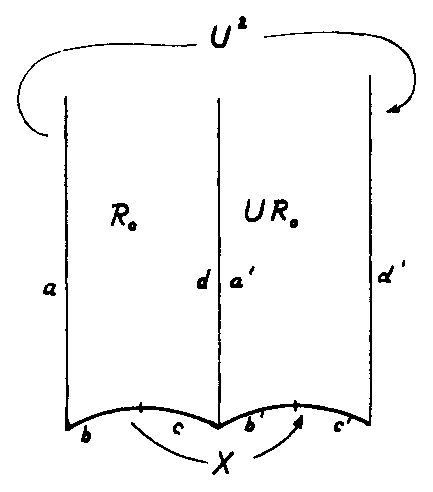
\includegraphics{chap07-vend-scan-15.eps}
\end{figure}

\subsection{}\label{ch07:sec6G}
The subgroups of a discontinuous group are in 1-1 correspondence with a class of covering surfaces\index{subgroup of discontinuous group!and covering surface} of the Riemann surface of the group (cf. \ref{ch06:chap06}. \ref{ch06:sec1G}-\ref{ch06:sec1J}, \ref{ch06:sec3I}, \ref{ch06:sec3J}).


\begin{theorem*}
Given a function group $\Gamma$ with domain $\mathscr{D}$, let $\sigma$ be the projection $\mathscr{D}^{+}\rightarrow S=\Gamma\backslash \mathscr{D}^{+}$. Let $H$ be a subgroup of $\Gamma$, let $S_{1}=H\backslash \mathscr{D}^{+}$, and let $\sigma_{1}$ be the projection $\mathscr{D}^{+}\rightarrow S_{1}$. Finally, let $S_{1}^{\prime}=H\backslash \mathscr{D}$. Then there exists a projection mapping $\tau:S_{1}\rightarrow S$ such that
\begin{equation*}
\tag{$^{\ast}$} \sigma=\tau \circ \sigma_{1}
\end{equation*}
and $(S_{1}^{\prime}, \tau)$ covers $S$. \emph{(}That is, the three projections are consistent.\emph{)}

Conversely, if $S_{1}$ is a surface and $\sigma_{1},\,\tau$ are projections such that $(\mathscr{D}, \sigma_{1})$ covers $S_{i}^{\prime}, (S_{i}^{\prime}, \tau)$ covers $S$, and $(^{\ast})$ holds, there is a subgroup $H$ of $\Gamma$ such that
\begin{equation*}
H\backslash \mathscr{D}^{+}=S_{1}.
\end{equation*}
\end{theorem*}

We define $\tau$ by $(^{\ast})$, i.e.,
\begin{equation*}
\tau(q_{1})=\sigma\circ\sigma_{1}^{-1}(q_{1}),\qquad q_{1}\in S_{1}
\end{equation*}
and note that it is a single-valued mapping. For two points in $\sigma_{1}^{-1}(q_{1})$ are $H$-equivalent, hence $\Gamma$-equivalent, and so are mapped by $\sigma$ into the same point of $S$.

Suppose $q_{1}$ is a point of $S_{1}$ and $\sigma_{1}(z)=q_{1}$. Let $\sigma(z)=q$; then $\tau(q_{1})=q$. There is a neighborhood $N$ of $z$ such that $N-z$ is a smooth covering of $\sigma(N)-q$, and a neighborhood $N_{1}$ of $z$ such that $N_{1}-z$ is a smooth covering of $\sigma_{1}(N_{1})-q_{1}$. At each point of $N^{\prime}-z$, where $N^{\prime}=N\cap N_{1}$, both $\sigma$ and $\sigma_{1}$ are local homeomorphisms. Hence $\tau$ is a local homeomorphism from $\sigma_{1}(N^{\prime})-q_{1}$ to $\sigma(N^{\prime})-q$, showing that $(S^{\prime}_{1},\,\tau)$ is a branched covering of $S$. The direct part of the theorem is established.

To prove the converse, let $h$ be a covering transformation of $(\mathscr{D},\,\sigma_{1})$. That is, $h$ is a homeomorphism of $\mathscr{D}$ that satisfies
\begin{equation*}
\sigma_{1}\circ h=\sigma_{1}.
\end{equation*}
Applying $\tau$ to both sides and using $(^{\ast})$, we get
\begin{equation*}
\sigma\circ h=\sigma.
\end{equation*}
Hence $h$ is a covering transformation of $(\mathscr{D},\,\sigma)$. But by \ref{ch06:chap06}. \ref{ch06:sec3J} the group of these covering transformations is $\Gamma$ itself, so $h$ is an element of $\Gamma$. We now define $H$ to be the group of covering transformations of $(\mathscr{D},\,\sigma_{1})$; what we have just proved is that $H$ is a subgroup of $\Gamma$.

We can assert, again by \ref{ch06:chap06}. Th. \ref{ch06:sec3J}, that $H\backslash\mathscr{D} ^{+} = S_{1}$. For $\sigma_{1}$ maps $\mathscr{D}^{+}$ on $S_{1}$, identifying points that are equivalent under a certain group $H^{\ast}$. By the theorem cited, $H^{\ast}$ is the group of covering transformations of $\mathscr{D}$ relative to $S_{1}$ and so, by definition, is equal to $H$. Hence $\sigma_{1}$ identifies $H$-equivalent points, from which our assertion follows. This concludes the proof.

\subsection{}\label{ch07:sec6H}
We can use the last theorem to develop a formula for the genus of a subgroup.

Suppose $\Gamma$ is of finite genus $g$. Let us have a triangulation\footnote{The fact that a surface of finite genus can be triangulated is proved in \citeauthor{Springer0000}~[\ref{Springer1}\index{Springer}, p. 124].} of $S =\Gamma\backslash \mathscr{D}^{+}$ with $\alpha_{0}$ vertices, $\alpha_{1}$ sides, and $\alpha_{2}$ triangles; then by Euler's formula
\begin{equation*}
\tag{$^{\ast}$} \alpha_{0}-\alpha_{1}+\alpha_{2} =2-2g.
\end{equation*}
This triangulation induces one on the surface $S_{1}^{\prime}=H\backslash \mathscr{D}$ which, by Theorem 6G, covers $S$. If $(\Gamma:H)=\mu$, finite, there are evidently $\mu$ points on $S_{1}$ that project into a single point on $S$ except at the projection of a branch point. Thus if we denote the vertices, sides, and cells of the triangulation on $S_{1}$ by primed letters, we have
\begin{equation*}
\alpha_{1}^{\prime}=\mu\alpha_{1},\qquad \alpha_{2}^{\prime}=\mu \alpha_{2}.
\end{equation*}
The number of branch points is finite. For a branch point corresponds to a vertex of the fundamental region of $H$, which consists of $\mu$ copies of the fundamental region of $\Gamma$. But the latter has a finite number of sides, for $\Gamma$ is of finite genus.

It follows that we can select the triangulation of $S$ in such a way that the projection of a branch point is always a vertex. Denote by $n_{i}-1$ the order of the $i$th branch point (cf. \ref{ch06:chap06}. \ref{ch06:sec1J}). If we now define the \emph{ramification index}\index{ramification index} of $S_{1}$ relative to $S$ by
\begin{equation*}
V=\sum\,(n_{i}-1),
\end{equation*}
the sum being extended over all branch points of $S_{1}$, we have $\alpha_{0}^{\prime}=\mu\alpha_{0}-V$. Hence, writing $g^{\prime}$ for the genus of $H$, we get
\begin{equation*}
\mu\alpha_{0}-V-\mu \alpha_{1}+\mu \alpha_{2}=2-2g^{\prime},
\end{equation*}
and using $(^{\ast})$,
\begin{equation} \label{ch07:eqn13}
g^{\prime}-1=\frac{1}{2}V+\mu(g-1).
\end{equation}

For an application of this formula to certain subgroups\index{subgroup of discontinuous group!genus of} of the modular group, cf. \ref{ch11:chap11}. \ref{ch11:sec3C}.


\subsection{}\label{ch06:sec6I}
\begin{theorem*}
Let $H$ be a subgroup of finite index in $\Gamma$. There exists a proper invariant on\index{subgroup of discontinuous group!proper invariant on} $H$, i.e., a function automorphic on $H$ but not automorphic on any $H_{1}$ for which $H\subset H_{1}\subset\Gamma$.
\end{theorem*}

Let $\{HA_{1},\,\cdots ,\,HA_{s}\}$ be a system of cosets of $H$ in $\Gamma$ and let
\begin{equation*}
z_{j}=A_{j}z_{0},\qquad j=1,\,\cdots ,\,s
\end{equation*}
$z_{0}$ being a fixed, arbitrary point. We introduce the Riemann surface $S$ of $H$ and denote by $q_{j}$ the projection of $z_{j}$ in $S$. The points $\{q_{j}\}$ are distinct. For $j=1,\,\cdots,\,s$, let $\varphi_{j}$ be a function on $S$ with a pole at $q_{j}$ and otherwise regular (cf. \ref{ch06:chap06}. \ref{ch06:sec2J}). Then
\begin{equation*}
\psi_{j}(q)=\prod_{i\neq j}(\varphi_{j}(q)-\varphi_{j}(q_{i}))
\end{equation*}
has a pole at $q_{j}$ and a zero at $q_{i},\,i\neq j$. Hence
\begin{equation*}
\omega_{j}(q)=\frac{\psi_{j}(q)}{1+\psi_{j}(q)}
\end{equation*}
is a function on $S$ which takes the value 1 at $q_{j}$ and the value $0$ at $q_{i}\neq q_{j}$.

Let $f_{j}(z)$ be the automorphic function on $H$ corresponding to $\omega_{j}$ (cf. \ref{ch06:chap06}. Th. \ref{ch06:sec4A}). Let $c_{1},\,\cdots,\,c_{s}$, be distinct complex numbers. The function
\begin{equation*}
f(z)=\sum\limits_{j=1}^{s}c_{j}f_{j}(z)
\end{equation*}
plainly assumes the value $c_{j}$ at $z=z_{j}$. Thus the values $\{f(z_{j}),j=1,\, \cdots,\, s\}$ are all different: $f$ ``separates'' the points $z_{1},\,\cdots,\,z_{s}$.

Now suppose $H\subset H_{1}\subset\Gamma$, and $H\backslash H_{1}=\{HB_{1},\,\cdots,\,HB_{t}\}$. Since $B_{j}\in\Gamma$, we have
\begin{equation*}
B_{j}=T_{j}A_{k},\qquad j=1,\,\cdots,\,t
\end{equation*}
where $T_{j}\in H$ and $k=k(j)$. Therefore
\begin{equation*}
f(B_{j}z_{0})=f(A_{k}z_{0})=f(z_{k}).
\end{equation*}
But $A_{k}\neq I$ for all $j$, otherwise $H_{1}$ would be a subgroup of $H$. Hence for some $j,\, f(B_{j}z_{0})\neq f(z_{0})$, showing that $f$ is not invariant on $H_{1}$.


\skiptoctrue
\section*{Exercises}

1. The group\index{Hecke group|(} $G$ generated by $a,\,b,\,c$ with the defining relation\index{relations in a group|(} $abc=1$ is isomorphic to the free group $F_{2}$ on $a,\,b$. Generalize to the case discussed near the end of 6A. [$G$ is isomorphic to $F_{3}/N$, where $F_{3}$ is the free group on $a,\,b,\,c$ and $N$ is the smallest normal subgroup of $F_{3}$ containing the word $abc$. Cf. \ref{ch02:chap02}. \ref{ch02:sec5C}. Consider the mapping of $F_{3}/N$ on $F_{2}$ determined by $Na\rightarrow a,\,Nb\rightarrow b,\,Nc\rightarrow b^{-1}a^{-1}.]$

2. Let $\Gamma$\index{$\Gamma^{2}\cdot\Gamma^{3}$} be a group containing\index{subgroup of discontinuous group!existence of \_\_\_s of given index|(} two elliptic generators of orders $l_{1},\,l_{2}$. If $d>1$ is the greatest common divisor of $l_{1}$ and $l_{2}$, the construction of 6A yields a normal subgroup of index $d$.

3. Klein\index{Klein} made the following definition. Let $n>1$ be an integer and let $X=\{X_{i},\,i=1,\,2,\, \cdots,\,s\}$ be a system of elements of the modular group such that $X_{i}X_{j}^{-1}\equiv X_{k}(\mathrm{mod}\,n)$ for each $(i,j)$ and some $k,\,1\leqq i,j,\,k\leqq s$. The set $\Gamma$ consisting of all matrices congruent modulo $n$ to some $X_{i}$ is called an inhomogeneous congruence group\index{congruence subgroup|(} of level $n$. Show this definition is equivalent to ours (6B). [If the condition is satisfied, one of the $X_{i}$'s must be the identity. Conversely, if $\overline{\Gamma}(n)\subset\overline{\Gamma}$. note that $\overline{\Gamma}(n)$ is normal in $\overline{\Gamma}$. Study $\overline{\Gamma}/\overline{\Gamma}(n).]$

4. The genus of a subgroup of finite index is at least equal to the genus of\index{subgroup of discontinuous group!genus of|(} the group. If the genus of the group is positive, it is less than the genus of the subgronp.

5. The Hecke\index{Hecke} group $\Gamma(\lambda)$---cf.\,\ref{ch07:sec6E}---is not an $SL(2,\,R)$ for any ring $R$.

\section{Subgroups and Subfields}\index{subgroup of discontinuous group!and subfield}\label{ch07:sec7}

Let $\Gamma$ be a function group, $\Delta$ a normal subgroup of finite index in $\Gamma$. Let $\mathbf{K}(\Gamma),\, \mathbf{K}(\Delta)$ be the fields of\index{automorphic functions of $n$ variables!field of} automorphic functions on $\Gamma$ and $\Delta$, respectively. The theorem of this Section considers\index{field of automorphic functions!normal extension of} the relation of $\mathbf{K}(\Gamma)$ to $\mathbf{K}(\Delta)$.

\subsection{}\label{ch07:sec7A}
We recall some elementary notions from field theory.\footnote{Cf., e.g., van der\index{Waerden, van der} [\citeauthor{Waerden0000}~\ref{Waerden1}, Ch.~\ref{ch05:chap05}]; we assume the field characteristic is 0.} If $F$ is a subfield of $E$, we shall call $E$ an extension field of $F$. The element $g\in E$ is said to be algebraic over $F$ if $g$ is the root of a polynomial over $F$ (i.e., with coefficients in $F)$. Among all the polynomials over $F$ of which $g$ is a root, there is one which is of lowest degree (hence irreducible) and has leading coefficient 1; it is called the \emph{minimum polynomial} and its degree is the \emph{degree of} $g$. The field $E$ is said to be a simple algebraic extension\index{automorphic functions of $n$ variables!algebraic dependence of} or a finite extension of $F$ if\footnote{$F(g)$ is the field of rational functions of $g$ with coefficients in $F$.} $E =F(g)$ for some $g$ which is algebraic over $F$. We say $g$ generates $E$; the \emph{degree of} $E$ is defined to be the degree of $g$. If $E$ is of degree $\mu$, it is generated by any element of degree $\mu$.

Let $E$ be a finite extension of $F$. Two elements $h,\,k$ of $E$ are said to be conjugate over $F$ if they are roots of the same minimum polynomial over $F$. The extension $E$ is said to be normal over $F$ if it contains all conjugates over $F$ of each of its elements. The Galois group of a normal extension $E$ of $F$ is defined to be the group of all automorphisms of $E$ that leave each element of $F$ fixed.


\subsection{}\label{ch07:sec7B}
We now let $\Gamma$\index{compactness modulo $\Gamma$} be a function group. For the field $F$ we choose $\mathbf{K}(\Gamma)$, the field of automorphic functions on $\Gamma$. Let $E =F(g)$ be a field of automorphic functions that is a normal extension of $F$ of finite degree $\mu$. Each element $h$ of $E$ satisfies an irreducible algebraic equation $P=0$ over $F$ of degree $\nu\leqq\mu$. Denote the conjugates of $h$ by $h_{1},\,h_{2},\,\cdots,\, h_{\nu}$; one of these is of course equal to $h$. As the root of a polynomial equation over $F,\,g$ is an analytic function and the same is true of the conjugates $\{h_{i}\}$.

Consider $g=g(z)$, a generator of $E$. Denote by $\Delta$ the set of elements in $\Gamma$ under which $g$ is invariant:
\begin{equation*}
\Delta=\{T\in\Gamma|g(Tz)=g(z)\}.
\end{equation*}
Then $\Delta$ is a subgroup of $\Gamma$, consisting possibly of the identity alone. Write
\begin{equation*}
\Delta\backslash \Gamma=\{\Delta A_{1},\,\cdots,\,\Delta A_{s}\};
\end{equation*}
here $s$ may be infinite. Each element of $E$ is likewise invariant under $\Delta$, for it is a rational function of $g$.

Let $P=0$ be the irreducible algebraic equation satisfied by $g$. Since the coefficients of $P$ are in $F$ and hence invariant under $z\rightarrow A_{i}z$, we see that $\{g(A_{i}z),\,i=\,1,\,\cdots,\,s\}$ are conjugates of $g$. These conjugates are all distinct, for from $g(A_{i}z) =g(A_{j}z), i\neq j$, we could conclude, by replacing $z$ by $A_{j}^{-1}z$, that $g(A_{i}A_{j}^{-1}z) =g(z)$, or $A_{i}A_{j}^{-1}\in\Delta$.

However, there are exactly $\mu$ solutions of $P=0$, since $E$ is of degree $\mu$ and is generated by $g$. Hence
\begin{equation*}
 \tag{$^{\ast}$} s\leqq\mu.
\end{equation*}

Furthermore, $\Delta$ is a normal subgroup. Since $g(A_{i}z)$ is a conjugate of $g$, it belongs to $E$ and so is invariant under $\Delta$. Hence $g(A_{i}Tz)=g(A_{i}z)$ or $g(A_{i}TA_{i}^{-1}z)=g(z)$ for each $T\in\Delta$. But $\Delta$ contains \emph{all} transformations under which $g$ is invariant. It follows that $A_{i}TA_{i}^{-1}\subset\Delta$, whence $A_{i}\Delta A_{i}^{-1}\subset\Delta$. But every $V\in\Gamma$ is of the form $TA_{i}$ with $T\in\Delta$. Hence
\begin{equation*}
V\Delta V^{-1}=TA_{i}\Delta A_{i}^{-1}T^{-1}\,\subset T\Delta T^{-1}=\Delta,
\end{equation*}
and so $\Delta$ is normal (cf. \ref{ch02:chap02}. \ref{ch02:sec5A}).

We can now show $s=\mu$. Consider the polynomial
\begin{equation*}
P=(t-g(A_{1}z))\cdots(t-g(A_{s}z)),
\end{equation*}
of which $g$ is a zero. Each coefficient of $P$ is a symmetric function $\mathscr{S}$ of the $\{g(A_{i}z), i=1,\,\cdots,\,s\}$. Let $V\in\Gamma$; we have $V=A_{k}T$ for some $k$ and some $T\in\Delta$. Hence
\begin{align*}
&\mathscr{S}\{g(A_{1}Vz),\,\cdots,\,g(A_{s}Vz)\}=\mathscr{S}\{g(A_{1}A_{k}Tz),\,\cdots,\, g(A_{s}A_{k}Tz)\}\\
&\qquad\qquad\ =\mathscr{S}\{g(A_{1}Tz)),\,\cdots\,,g(A_{s}Tz)\}=\mathscr{S}\{g(A_{1}z),\,\cdots,\, g(A_{s}z)\},
\end{align*}
since $\{A_{1}A_{k},\,\cdots,\,A_{s}A_{k}\}$ is a permutation of $\{A_{1},\,\cdots,\,A_{s}\}$. Hence the coefficients of $P$ are invariant under $\Gamma$ and lie in $F$. This shows that the irreducible polynomial\index{automorphic functions of $n$ variables!as quotient of Poincar\'{e} series} of which $g$ is a root has degree $\leqq s$, but the degree of this polynomial is $\mu$. Therefore $\mu\leqq s$ which, with $(^{\ast})$, gives $s=\mu$.


\subsection{}\label{ch07:sec7C}
We have shown that each normal extension $E$ of $F =\mathbf{K}(\Gamma)$ of finite degree $\mu$ determines a subgroup $\Delta$ of index $\mu$ in $\Gamma$ such that all elements of $E$ are $\Delta$-invariant. In other words $E\subset \mathbf{K}(\Delta)$. It follows that
\begin{equation*}
\mu=\deg E\leqq\deg \mathbf{K}(\Delta).
\end{equation*}

Let $h\in \mathbf{K}(\Delta)$ but $h\not\in \mathbf{K}(\Delta^{\prime})$ for $\Delta\subseteq\Delta^{\prime}\subset\Gamma$ (cf. \ref{ch06:sec6I}). The functions $\{h(A_{i}z),\,i=1,\,\cdots,\,\mu\}$ are all distinct, for $h(A_{i}z)=h(A_{j}z)$ implies $A_{i}A_{j}^{-1}\in\Delta$. The polynomial
\begin{equation*}
(t-h(A_{1}z))\,\cdots\,(t-h(A_{\mu}z))
\end{equation*}
has $h(z)$ for a root and is of degree $\mu$. Each of its coefficients is a symmetric function of the $\{h(A_{i}z)\}$, and by the same reasoning as before we conclude the coefficients are $\Gamma$-invariant and so lie in $F$. This shows the degree of $\mathbf{K}(\Delta)$ cannot exceed $\mu$ and so is equal to $\mu$. Hence $E$ and $\mathbf{K}(\Delta)$ are of the same degree over $F$, and from $E \subset \mathbf{K}(\Delta)$ we can conclude that the two fields are identical. We have proved the first half of the following result:


\begin{theorem*}
If $E$ is a normal extension of $F=\mathbf{K}(\Gamma)$ of finite degree $\mu$, there is a normal subgroup $\Delta$ of index $\mu$ in $\Gamma$ such that $E=\mathbf{K}(\Delta)$. Conversely, for each normal subgroup $\Delta$ of finite index $\mu$ \emph{in} $\Gamma$, the field $\mathbf{K}(\Delta)$ is a normal extension of $\mathbf{K}(\Gamma)$ of degree $\mu$.
\end{theorem*}

To prove the converse, let us assume we have given a normal subgroup $\Delta$ of finite index $\mu$ in $\Gamma$; let $\Gamma/\Delta=\{A_{1},\,\cdots,\,A_{\mu}\}$. Suppose $h\in \mathbf{K}(\Delta)$. We have just seen that $h$ is algebraic over $F$ of degree at most $\mu$. Setting $E =\mathbf{K}(\Delta)$, we have that $E$ is a finite extension of $F$.

The degree of $E$ over $F$ is $\mu$ or less. We must show it is $\mu$. Let $g$ be invariant on $\Delta$ but not invariant on any $\Delta^{\prime}$ that lies between $\Delta$ and $\Gamma$ (cf. Th. \ref{ch06:sec6I}). The functions $\{g(A_{i}z),\,i=1,\,2,\,\cdots,\,\mu\}$ are all distinct, otherwise $g(A_{j}A_{k}^{-1}z) =g(z)$ for some $j\neq k$ and this contradicts the fact that $A_{j}A_{k^{-1}}\not\in\Delta$. Since these functions are conjugates over $F,\,g$ is of degree at least $\mu$. This proves $E$ is of degree at least $\mu$, hence of degree $\mu$.

It remains to prove $E$ is normal over $F$. The element $g$ referred to above is of degree $\mu$ and therefore generates $E$. The functions $\{g(A_{i}z), i=1,\,\cdots,\,\mu\}$ belong to $E$ because they are $\Delta$-invariant. If now $h\in E$ is arbitrary, we can write $h=R(g)$, where $R$ is a rational function over $F$. The coefficients of $R$ are $\Gamma$-invariant and so
\begin{equation*}
h(A_{i}z)=R(g(A_{i}z)),
\end{equation*}
showing that $h(A_{i}z)\in E$. This concludes the proof.

The content of the theorem is expressed by the commutativity of the following diagram:

\begin{figure}[!h]
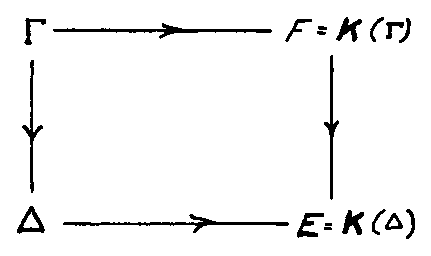
\includegraphics{chap07-vend-scan-16.eps}
\end{figure}

\subsection{}\label{ch07:sec7D}
We remark finally that $G =\Gamma/\Delta$ is isomorphic to the Galois group of $E$ over $F$.

The elements of $G$ are the cosets $\Delta A_{i},\,i=1,\,\cdots,\,\mu$. To $\Delta A_{i}$ we make correspond a mapping
\begin{equation*}
\tau_{i}\,:\,h(z)\rightarrow h|\tau_{i}=h(A_{i}z),\qquad h\in E.
\end{equation*}
$G$ is isomorphic to the group $\{\tau_{i}\}$ with the multiplication $h\,|\,\tau_{i}\tau_{j}=h(A_{i}A_{j}z)$.

We verify without difficulty that $h(A_{i}z), h(A_{i}^{-1}z)$ are $\Delta$-invariant. Hence $\tau_{i}$ is from $E$ into $F$; it is also \emph{onto} $E$, for $h\in E$ implies
\begin{equation*}
h(z)=h(A_{i}\circ A_{i}^{-1}z)=h(A_{i}^{-1}z)|\tau_{i}.
\end{equation*}
Finally, $h |\tau_{i}=k|\tau_{i}$ implies $h=k$, as we see by replacing $z$ by $A_{i}^{-1}z$. The mapping $\tau_{i}$, then, is 1-1 from $E$ to itself. That it preserves sums and products is trivial: $\tau_{i}$ is an automorphism of $E$.

Since $\tau_{i}$ certainly leaves each element of $F$ invariant, we conclude that $G$ is isomorphic to a subgroup of the Galois group $\mathfrak{G}$ of $E$ over $F$.

Both $G$ and $\mathfrak{G}$ are of order $\mu$. Hence $G\cong\mathfrak{G}$.


\begin{theorem*}
If $\Delta$ is normal and of finite, index in $\Gamma$, the Galois group of $\mathbf{K}(\Delta)$ over $\mathbf{K}(\Gamma)$ is isomorphic to $\Gamma/\Delta$.
\end{theorem*}

\subsection{}\label{ch07:sec7E}
Let us give one application of our result, Theorem 7C. The principal congruence subgroup\index{modular group} $\Gamma(2)$ is of index 6 in $\Gamma(1)$ and has a fundamental region $R_{0}$ bounded by the vertical lines $x=\pm 1,\,y>0$ and the circles of diameter 1 through $-1,0$ and $0,1$. It has two generators conjugating the vertical sides and circular arcs, respectively, and so is of genus 0 (cf. \ref{ch11:chap11}. \ref{ch11:sec3B}). Therefore, there is a univalent function on $\Gamma(2)$---cf. \ref{ch06:chap06}. Th. \ref{ch06:sec2K}---and we denote by $\lambda(\tau)$ the function which takes the values
\begin{equation*}
\lambda(-1)=\infty,\qquad \lambda(0)=1,\qquad \lambda(\infty)=0.
\end{equation*}\index{principal congruence subgroup!mod 2}
Since $\lambda$ assumes the value $0$ exactly once in a fundamental set, it follows that $\lambda(\tau)$ \emph{is never zero in} $R_{0}$.

Thus we can define $g(\tau)=(\lambda(\tau))^{1/n}$ as a single-valued analytic function. The polynomial
\begin{equation*}
P(t)=t^{n}-\lambda
\end{equation*}
is irreducible over $F=\mathbf{K}(\Gamma(2))$ and has $g$ as a root. It defines an extension $E=F(g)$ of $F$ of degree $n$. $E$ is normal over $F$, for the conjugates of $g$ are constant multiples of $g$ and also lie in $E$. By our theorem there is a normal subgroup $\Gamma_{n}$ of $\Gamma(2)$ such that
\begin{equation*}
\mathbf{K}(\Gamma_{n})=E=F(\lambda^{1/n}).
\end{equation*}
One of the interesting features of this family of subgroups is that only for a finite number of values of $n$ is $\Gamma_{n}$ a congruence subgroup, although all $\Gamma_{n}$ are of finite index. In fact $\Gamma_{n}$ is closely related to the groups $\Omega_{n}$ of 6C.


\textit{Warning}: We cannot apply the same process unrestrictedly to $j(\tau)$\index{$j(\tau)$}, Klein's absolute invariant of the modular group (\ref{ch11:chap11}. \ref{ch11:sec1E}). For $j$ has a zero of order 3 at $\tau=e(1/3)$ and is otherwise zero-free; thus the only single-valued root we can define is $j^{1/3}$. Likewise, $j(\tau)-1728$ has a double zero at $\tau=i$ and no other zeros; we can therefore define $(j(\tau)-1728)^{1/2}$. The function $j$, then, can be used to construct two normal subgroups of $\Gamma(1)$ of indices 3 and 2, corresponding to the normal extensions $\mathbf{K}(j^{1/3}),\,\mathbf{K}((j-1728)^{1/2})$, respectively.

%%%%%%%%%chapter08

\chapter{Forms of Negative Dimension}\label{ch08:chap08}\index{automorphic forms of negative dimension}

\section{Introduction}\label{ch08:sec1}

\subsection{}\label{ch08:sec1A}
The bulk of the work in the theory of automorphic functions has always been on principal-circle groups. Since about 1925 these have been investigated mostly in the upper half-plane $\mathscr{H}$. For such groups we can choose the coefficients of the transformations to be real (\ref{ch02:chap02}. \ref{ch02:sec9E}). Moreover it is usually assumed that the group has translations. This is because the case of the modular group and its subgroups is of central importance, the more so since the discovery by Hardy\index{Hardy} and Ramanujan\index{Ramanujan}\index{Hardy-Ramanujan} in 1917 that these groups and their analytical invariants can be successfully applied to important problems of number theory. (Cf.~\ref{ch01:chap01}.~\ref{ch01:sec4}.) An essential feature of this class is that there is a fundamental region with a finite number of sides. This implies that the group is finitely presented (i.e., has a finite system of generators and relations). We are thus led to a class of discontinuous groups that we shall call $H$-groups.\index{$H$-group}


\begin{definition*}
$\Gamma$ is an $H$-group provided

1) $\Gamma$ is discontinuous in the upper half-plane $\mathscr{H}$ but is not discontinuous at any point of the real axis

2) $\Gamma$ has translations (parabolic elements with fixed point $\infty$)

3) $\Gamma$ has a fundamental region $R_{0}$ with a finite number of sides.

\noindent Petersson\index{Petersson} calls an $H$-group ``Grenzkreisgruppe erster Art mit $\sigma_{0}>0$.'' Rankin\index{Rankin} calls a group satisfying 1) and 2) a ``real zonal horocyclic group.''

An $H$-group is a principal-circle group and the fundamental theory developed in Chapters~\ref{ch03:chap03} and~\ref{ch04:chap04} applies to $H$-groups. However, for several reasons it is desirable to work out their theory anew. In order to apply the previous results we have to consider not $\Gamma$ but $A\Gamma A^{-1}$, where $A$ sends to $\infty$ some ordinary point of $\mathscr{H}$ that is not a fixed point. Thus $A$ is not real, and the coefficients of the matrices of $A\Gamma A^{-1}$ are no longer real and certainly stand in no simple relationship to those of $\Gamma$. This is a serious disadvantage if, for example, we are interested in arithmetic applications. Moreover, the reality of the coefficients of $\Gamma$ is in itself a desirable simplification, the appropriate Poincar\'{e} series takes a new and more elegant form, and so on. We shall therefore make a fresh start in this chapter, using, of course, our previous results whenever possible.
\end{definition*}

\subsection{}\label{ch08:sec1B}
Dedekind\index{Dedekind} and Hermite\index{Hermite} introduced the $\eta$-function
\begin{equation*}
\eta(\tau)=e(\tau/24)\prod\limits_{m=1}^{\infty}\,(1\,-e(m\tau)),\qquad \mathrm{Im}\
\tau>0
\end{equation*}
and worked out its transformation formula:
\begin{equation*}
\tag{$^{\ast}$} \eta(M\tau)=v_{0}(M)(c\tau+d)^{1/2}\eta(\tau),\qquad \tau\in \mathscr{H}
\end{equation*}
where $M$ is any modular substitution and $v_{0}(M)$ is a certain 24th root of unity whose dependence on the coefficients of $M$ is very complicated (\ref{ch11:chap11}. Th. \ref{ch11:sec1C}). The function $v_{0}(M)$ is called a \emph{multiplier}. Clearly $\eta$ is regular in\footnote{$\mathscr{H}^{+}=\mathscr{H}\cup\mathscr{P}$; $\mathscr{P}$ is the set of parabolic vertices of $\Gamma$.} $\mathscr{H}^{+}$. Looking at $(^{\ast})$ we would say that $\eta$ is an automorphic form of dimension $-1/2$, except for the factor $v_{0}(M)$. On the other hand, it appears from \ref{ch06:chap06}. Th. \ref{ch06:sec4C} that there is no single-valued nonconstant analytic function, regular in $\mathscr{H}^{\,+}$, which satisfies $(^{\ast}$) with $v_{0}(M)\equiv 1$. Indeed if $f$ is such a function, $f^{4}\in \mathbf{C}^{+}(\Gamma(1),\, -2)$ and the dimension of this space is 0. That is, there is no everywhere regular automorphic form of dimension $-1/2$ in the sense of our definition in \ref{ch05:chap05}. 1B. Hence we extend our definitions. We do this with no reluctance, for we see that multipliers arise in a natural way in our study of actual groups and their invariant functions.

The multiplier $v_{0}(M)$, besides being of unit absolute value, has the property that, for any substitutions $M_{1},\,M_{2}$,
\begin{equation*}
\tag{$^{\ast\ast}$} v_{0}(M_{1}M_{2})(c_{12}\tau+d_{12})^{1/2}=v_{0}(M_{1})(c_{1}M_{2}\tau+d_{1})^{1/2}v_{0}(M_{2})(c_{2}\tau+d_{2})^{1/2},
\end{equation*}
where
\begin{equation*}
\tag{$\dagger$} M_{i}=\left(\begin{matrix}
\cdot & \cdot\\
c_{i} & d_{i}
\end{matrix}\right),\quad i=1,\,2;\qquad M_{1}M_{2}=\left(\begin{matrix}
\cdot & \cdot\\
c_{12} & d_{12}
\end{matrix}\right).
\end{equation*}
Here a many-valued function appears and we fix its value by our standard convention,~\ref{ch02:chap02}.~\ref{ch02:sec7H}. The relation $(^{\ast\ast})$ is obtained by evaluating $\eta(M_{1}M_{2}\tau)$ in two ways:
\begin{gather*}
\eta(M_{1}M_{2}\tau)=v_{0}(M_{1}M_{2})(c_{12}\tau+d_{12})^{1/2}\,\eta(\tau),\\
\eta(M_{1}M_{2}\tau)=\eta(M_{1}(M_{2}\tau))=v_{0}(M_{1})(c_{1}M_{2}\tau+d_{1})^{1/2}\,\eta(M_{2}\tau)\\
\quad\ \ \qquad=v_{0}(M_{1})(c_{1}M_{2}\tau+d_{1})^{1/2}v_{0}(M_{2})(c_{2}\tau+d_{2})^{1/2}.
\end{gather*}
Since $\eta(\tau)\not\equiv 0$ we get $(^{\ast\ast})$ by comparing the two equations.


We use these properties as the basis for our definition of a \emph{multiplier system}\index{multiplier system}:

\begin{definition*}
We say that $v=v[\Gamma,\,-r]$ is a multiplier system\index{multiplier system!existence of} for the $H$-group\index{$H$-group} $\Gamma$ and the dimension $-r$ provided $v(M)$ is a complex-valued function defined on $M\in\Gamma$ such that
\begin{align}
\mathrm{i)}\quad &|v(M)|=1,\nonumber\\
\label{ch08:eqn1} \mathrm{ii)}\quad &v(M_{1}M_{2})(c_{12}\tau+d_{12})^{r}=v(M_{1})(c_{1}M_{2}\tau+d_{1})^{r}\,v(M_{2})(c_{2}\tau+d_{2})^{r},
\end{align}
where $M_{1},\,M_{2}\in\Gamma$ and $M_{1}M_{2}$ have the coefficients in $(\dagger)$.
\end{definition*}

We can now define an automorphic form.

\begin{definition*}
Let $v=v\lfloor\Gamma,\,-r\rfloor$. An automorphic form on $\Gamma$ of dimension $-r$ and multiplier system $v$ is a function $F(\tau)$, meromorphic in $\mathscr{H}^{+}$, which satisfies there the transformation equation
\begin{equation}\label{ch08:eqn2}
F(M\tau)=v(M)(c\tau+d)^{r}F(\tau)
\end{equation}
for each $M=(\cdot\ \cdot|c\,d)\in\Gamma$.
\end{definition*}

We shall have to specify, as we did in \ref{ch05:chap05}. \ref{ch05:sec1B}, just what we mean by meromorphicity at points of $\mathscr{P}$.

The set of all forms $F$ on $\Gamma$ of dimension $-r$ and multiplier system $v$ forms a complex vector space denoted by $\{\Gamma,\,-r,\,v\}$\index{$\{\Gamma,\,-r,\,v\}$}.

It is clear that the existence of a nonconstant function $F$ satisfying \eqref{ch08:eqn2} for all $M\in\Gamma$ and certain values $v(M)$ with $|v|=1$ defines $v$ as a multiplier system belonging to $\Gamma$ and $-r$.

When $r$ is an integer, \eqref{ch08:eqn1} reduces to
\begin{equation}\label{ch08:eqn3}
v(M_{1}M_{2})=v(M_{1}) v(M_{2}).
\end{equation}
In other words, $v(M)$ is a \emph{character} of the group $\Gamma$, i.e., a homomorphism of $\Gamma$ into the multiplicative group of complex numbers of modulus 1. There is no difficulty in establishing the existence of multiplier systems in this case. In fact, since the fundamental region $R_{0}$ has a finite number of sides, $\Gamma$ is finitely presented and its independent relations are of the form \ref{ch07:chap07}. \eqref{ch07:eqn6}. Let
\begin{equation*}
\Gamma=\{S_{i},\,i=1,\,\cdots,\,s;\quad \mathbf{R}_{j},\,j=1,\,2,\,\cdots,\,t\}.
\end{equation*}
Define $v$ arbitrarily on the generators subject only to the requirements $|v|=1,\,v(I)=1,\, v(S_{i}^{-1})=1/v(S_{i})$, and $v(\mathbf{R}_{j})=1$. Thus in particular $v(E_{i})$ will be an $l_{i}$-th root of unity. Now extend $v$ to the whole group by homomorphism. That is, if $M=S_{1}S_{2}\cdots S_{m}$, define $v(M)=v(S_{1}) v(S_{2})\cdots v(S_{m})$. It is clear that $v$ is now uniquely defined. For if $M$ is written in two ways, $M=W_{1}=W_{2}$, the $W$'s being words in the generators, we have $W_{1}W_{2}^{-1}=I$; hence
\begin{equation*}
W_{1}=W_{2}\cdot T_{1}\mathbf{P}_{1}T_{1}^{-1}\cdots T_{k}\mathbf{P}_{k}T_{k}^{-1},\quad T_{i}\in\Gamma,\quad \mathbf{P}_{i}=\mathbf{R}_{j}^{\epsilon},\quad\epsilon=\pm 1
\end{equation*}
whence $v(W_{1})=v(W_{2})$. It is also easily checked that $v$ satisfies i) and ii).

Note that a $v[\Gamma,\,-r_{0}]$ is a $v[\Gamma,\,-r]$ for every integer $r$.

The situation is far different when $r$ is not an integer. The relation \eqref{ch08:eqn1} is no longer purely group-theoretic, and its iteration becomes highly involved. In short, it is by no means obvious that multiplier systems exist. When Hecke wrote on the subject, he made use of the multipliers which arose naturally from the special functions (e.g., theta functions) which occurred in the investigation. In 1930 Petersson\index{Petersson}, adopting a more abstract point of view, proved the existence of multiplier systems for arbitrary groups and dimensions (\citeauthor{Petersson0000}~[\ref{Petersson1}, pp. 431ff.]).

Once we have the multiplier systems it is possible, as Petersson showed, to carry over the entire theory of Poincar\'{e} series to arbitrary real dimension $<-2$. (\citeauthor{Petersson0000}~[\ref{Petersson1}].) This is an interesting generalization and it can be carried through in a straightforward manner once certain preliminaries are out of the way. However, the details are very tedious and their presence obscures the main ideas of the development. For this reason we shall confine ourselves to integral dimension. When we treat forms of positive dimension in the next chapter, we shall allow $r$ to be nonintegral, since in Chapter~\ref{ch11:chap11} forms of positive half-integral dimension will arise. \emph{In this chapter we assume} $r$ \emph{integral}.

\subsection{}\label{ch08:sec1C}
The present theory of automorphic\index{$P_{j}$|)} forms of negative dimension on $H$-groups is based mainly on two developments, both due to Petersson:\index{Petersson} a new type of Poincar\'{e} series, and the norming of the space $\{\Gamma,\,-r,\,v\}$ so that it becomes a Hilbert space. The present chapter is devoted to an exposition of this theory.
\index{Poincar\'{e} series on $H$-group!Fourier coefficients of|(}

\section{\textit{H}-Groups}\label{ch08:sec2}

In this Section we develop the properties of $H$-groups\index{discontinuous group in $n$ variables} that are needed for this and the next chapter.

\subsection{}\label{ch08:sec2A}
Let $\Gamma$ be an $H$-group. The elements of $\Gamma$ will be written as matrices $M=(a\,b\,|\,c\,d)$ with real $a,\,b,\,c,\,d,\,ad\,-\,bc=1$. We shall agree that $\Gamma$ contains $-I=(-1\,0\,|\,0\,-1)$. If not, $-I$ can be adjoined (cf. \ref{ch02:chap02}. \ref{ch02:sec11A}).

No loxodromic elements occur in $\Gamma$ since $a+d$ is real. By definition $\Gamma$ contains parabolic elements. $\Gamma$ may or may not contain elliptic substitutions.\index{discontinuous group!is countable} But it must contain hyperbolic elements (\ref{ch03:chap03}.~\ref{ch03:sec2D}).

The fixed points of a parabolic or hyperbolic transformation are real; those of an elliptic transformation are complex conjugate nonreal numbers.

Let $A$ be real unimodular, $Ap=\infty$ for a fixed point $p$. Then $A$ maps $\mathscr{H}$ on itself, and $AMA^{-1}$ is parabolic with fixed point $\infty$ if $M$ is parabolic with fixed point $p$. Hence $A\,\Gamma A^{-1}$ is an $H$-group.


\subsection{}\label{ch08:sec2B}
Let $\mathscr{P}$ be the set of parabolic vertices of $\Gamma$, and let $p\in \mathscr{P}$; $p$ is real. The subgroup $\Gamma_{p}$ (consisting of those elements of $\Gamma$ that fix $p$) is cyclic (\ref{ch04:chap04}. 6D). If $p$ generates $\Gamma_{p}$, so do $-P,\,\pm\, P^{-1}$. It is necessary to make a normalization.

For this purpose select a complete set of inequivalent parabolic vertices $p_{0},\,p_{1},\,\cdots,\,p_{s}$. If $\infty$ is one of the $p$'s, write $p_{0}=\infty$; otherwise $p_{0}$ does not occur. Since $\Gamma$ has a finite number of sides, $s$ is finite. Let $P_{j}$ be a generator of $\Gamma_{p_{j}}$. Define
\begin{equation}
\label{ch08:eqn4} A_{j}=\left(\begin{matrix}
0 & -1\\
1 & -p_{j}
\end{matrix}\right),\quad j>0;\qquad A_{0}=I.
\end{equation}
We have $A_{j}p_{j}=\infty$ for all $j$. Now $A_{j}P_{j}A_{j}^{-1}$ is parabolic and fixes $\infty$, hence is a translation:
\begin{equation}
\label{ch08:eqn5} A_{j}P_{j}A_{j}^{-1}=U^{\lambda_{j}},
\end{equation}
where we write symbolically
\begin{equation*}
U^{\alpha}=\left(\begin{matrix}
1 & \alpha\\
0 & 1
\end{matrix}\right),\quad U^{1}=U,\qquad \alpha\ \mathrm{real}.
\end{equation*}
We select that generator of $\Gamma_{p_{j}}$, and call it $P_{j}$, for which $\lambda_{j}>0$.

In particular, $\Gamma_{\infty}$ is generated by $U^{\lambda_{0}}$. Hence $M =(\cdot\ \cdot\,|\,0\ \cdot)$ implies $M=U^{\lambda_{0}q}$ for some integer $q$.


\subsection{}\label{ch08:sec2C}
We can now construct a fundamental region\index{$H$-group!fundamental region of} $R_{0}$ for $\Gamma$ by Ford's\index{Ford} method (\ref{ch04:chap04}.~\ref{ch04:sec5G}). Select a period strip $\xi \leqq x\leqq\xi +\lambda_{0},\,y\geqq 0$, where $\xi$ is arbitrary. Since $\Gamma_{\infty}$ is the infinite cyclic group $\{U^{\lambda_{0}}\},\,R_{0}$ will lie within the strip. It will be bounded below by a finite number of arcs of isometric circles. Laterally it is bounded by congruent lines $x=\xi,\,y\geqq y_{0}$ and $x=\xi +\lambda_{0},\,y\geqq y_{0}$ for some $y\geqq 0$. From now on let $p_{0},\,p_{1},\,\cdots,\,p_{s}$ denote a complete inequivalent set of parabolic vertices \emph{lying in} $\bar{R}_{0}$, with the understanding that $p_{0}=\infty$ is \emph{always} present.

For many purposes it is convenient to use a fundamental region $\tilde{R}$ having the property that each parabolic cycle consists of a single vertex. There is a parabolic sector (\ref{ch04:chap04}. \ref{ch04:sec4G}) at each vertex lying entirely within $\tilde{R}$. The existence of such a fundamental region was proved in \ref{ch04:chap04}.~\ref{ch04:sec7G} for groups defined on $\mathscr{U}$. In the present case map $\mathscr{H}$ \index{fundamental region!for $H$-group}on $\mathscr{U}$, determine a fundamental region for the transformed group, then map back on $\mathscr{H}$. Cf. Note 24, p. 407.


\subsection{}\label{ch08:sec2D}
As in the case of groups for which $\infty$ is an ordinary point, the numbers $c$ in $M=(\cdot\ \cdot\,|\,c\ \cdot)\in\Gamma$ form a discrete set, but the previous proof (\ref{ch03:chap03}. Th. \ref{ch03:sec1H}) no longer applies. We shall need a more general result. Define
\begin{equation}\label{ch08:eqn6}
C_{jk}=\left\{x\left|\left(\begin{matrix}
\cdot & \cdot\\
x & \cdot
\end{matrix}\right)\in A_{j}\Gamma A_{k}^{-1}\right.\right\},\qquad j,\,k=0,\,1, \cdots,\,s.
\end{equation}
(Note that $A_{j}\Gamma A_{k}^{-1}$ is not a group unless $j=k$.)


\begin{theorem*}
For each $(j,\,k)$, $C_{jk}$\index{$C_{jk}$}\index{$\tilde{c}_{jk}$} is a discrete set of real numbers.
\end{theorem*}

If the theorem is false, there is a sequence of different $c_{n}$ such that $c_{n}\rightarrow c$ (finite) and each $c_{n}$ occurs in $X_{n}=(a_{n}\,b_{n}\,|\,c_{n}\,d_{n})\in A_{j}\Gamma A_{k}^{-1}$. We may assume $c_{n}>0$, otherwise replace $X_{n}$ by $-X_{n}$. Hence $c\geqq 0$. Let $X_{n}=A_{j}M_{n}A_{k}^{-1}$. Then $M_{n}\in\Gamma$ and $Y_{n}=A_{j}P^{r_{n}}_{j}M_{n}P_{k}^{t_{n}}A_{k}^{-1}\in A_{j}\Gamma A_{k}^{-1}$ for arbitrary integers $r_{n},\, t_{n}$.

But from \eqref{ch08:eqn5} we calculate
\begin{equation*}
Y_{n}=U^{\lambda_{j}r_{n}}X_{n}U^{\lambda_{k}t_{n}}=\left(\begin{matrix}
a_{n}+\lambda_{j}r_{n}c_{n} & \\
c_{n} & d_{n}+\lambda_{k}t_{n}c_{n}
\end{matrix}\right)=\left(\begin{matrix}
a_{n}^{\prime} & b_{n}^{\prime}\\
c_{n} & d_{n}^{\prime}
\end{matrix}\right).
\end{equation*}
Hence we can choose $r_{n},\,t_{n}$ so that
\begin{equation*}
1\leqq a_{n}^{\prime}<1+\lambda_{j}c_{n},\qquad 1\,\leqq d_{n}^{\prime}<1+\lambda_{k}c_{n}.
\end{equation*}
Thus
\begin{equation*}
0\leqq b_{n}^{\prime}=\frac{a_{n}^{\prime}d_{n}^{\prime}-1}{c_{n}}<\lambda_{j}+\lambda_{k}+\lambda_{j}\lambda_{k}c_{n}\leqq\lambda_{j}+\lambda_{k}+\lambda_{j}\lambda_{k}(1+c)
\end{equation*}
for $n>N$. Thus the coefficients of $Y_{n}$ are bounded and on a certain subsequence they converge: $Y_{m}\rightarrow Y=(a\,b\,|\,c\,d)$.

Consider the sequence $T_{m}=Y_{m+1}^{-1}Y_{m}$. We have $T_{m}\rightarrow I$ and $\{T_{m}\}$ contains infinitely many different elements. For otherwise $T_{m}=I(m>N)$, i.e., $Y_{m}=Y_{m+1}\,(m>N)$, and this contradicts the fact that the $c_{m}$ are all different. Since $T_{m}=A_{k}W_{m}A_{k}^{-1}$ with $W_{m}\in\Gamma$, the existence of the sequence $\{T_{m}\}$ implies that $A_{k}^{-1}\Gamma A_{k}$ is not discrete; hence $\Gamma$ is not discrete.\:\:\:q.e.d.

In particular, $j=k=0$ implies $A_{j}\Gamma A_{k}^{-1}=\Gamma$. Then
\begin{equation}\label{ch08:eqn7}
C_{00}=\left\{x\left|\left(\begin{matrix}
\cdot & \cdot\\
x & \cdot
\end{matrix}\right)\in\Gamma\right.\right\}
\end{equation}
is a discrete set of real numbers. Let
\begin{equation}\label{ch08:eqn8a}
\tilde{c}_{jk}=\min\,\{|x|\,|x\in C_{jk},\,x\neq 0\}.
\end{equation}
According to the theorem just proved,
\begin{equation*}
\tilde{c}_{jk}>0,\qquad j,\,k=0,\,1,\,\cdots,\,s
\end{equation*}
In particular, for $M=(a\,b\,|\,c\,d)\in\Gamma$, we have $c\neq 0$ implies $|c|\geqslant\tilde{c}_{00}$.

For later use we shall need the set
\begin{equation}\label{ch08:eqn9}
D_{c}(j,\,k;\alpha,\,\beta)=\left\{d\left|\left(\begin{matrix}
\cdot & \cdot\\
c & d\\
\end{matrix}\right)\in A_{j}\Gamma A_{k}^{-1},\quad \alpha\leqq-\frac{d}{c}<\beta\right.\right\},\qquad
c\,\neq 0.
\end{equation}\index{$D_{c}(j,\,k;\alpha,\,\beta)$}

\begin{lemma*}
For each $c\in C_{jk}$ and each pair of real numbers $\alpha,\,\beta$, the set $D_{c}(j, k;\alpha,\,\beta)$ is a finite set.
\end{lemma*}

We have only to show that $D_{c}(j, k;-\infty,\,\infty)$ is discrete. If it is not, there is a sequence of different $d_{n}\rightarrow d$ (finite) such that there is a matrix $(\cdot\ \cdot\,|\,c\,d_{n})$ belonging to $A_{j}\Gamma A_{k}^{-1}$. Then we can prove by the argument used above that $\Gamma$ is not discrete. Cf. Note 25, p. 407.

\subsection{}\label{ch08:sec2E}
We shall need certain elementary properties of a multiplier system $v[\Gamma,\,-r]$. Since $v$ is a character of $\Gamma$, we have
\begin{equation}
\label{ch08:eqn10} v(I)=1,\qquad v(M^{-1})=1/v(M)=\overline{v}(M),\qquad v(M^{n})=(v(M))^{n},
\end{equation}
for $M \in\Gamma$. An element $M$ of finite order $l$ in $\Gamma$ has a multiplier $v(M)$ that is a $l$ th root of unity. In particular
\begin{equation*}
v(-I)=\pm\ 1.
\end{equation*}

Define $\kappa=\kappa_{j}(\Gamma)$ as the unique real number satisfying
\begin{equation}
\label{ch08:eqn11} e(\kappa_{j})=v(P_{j}),\qquad 0\leqq \kappa_{j}<1,\qquad
j=0,\,1,\,\cdots,\,s.
\end{equation}
Consider the group $\Gamma^{\prime}=A_{j}\Gamma A_{j}^{-1}$. The multiplier $v[\Gamma,\,-r]$ induces a multiplier $v^{\prime}[\Gamma^{\prime},\,-r]$ defined by
\begin{equation*}
v^{\prime}(M^{\prime})=v(M),\qquad M^{\prime}=A_{j}MA_{j}^{-1}.
\end{equation*}
Since $P_{j}$ generates $\Gamma_{p_{j}}$ while $A_{j}P_{j}A_{j}^{-1}$ generates $\Gamma_{\infty}^{\prime}$, we have
\begin{equation*}
e(\kappa_{j})=v(P_{j})=v^{\prime}(A_{j}P_{j}A_{j}^{-1})=e(\kappa_{0}\,(\Gamma^{\prime}));
\end{equation*}
hence
\begin{equation}
\label{ch08:eqn12} \kappa_{j}(\Gamma)=\kappa_{0}(A_{j}\Gamma A_{j}^{-1}).
\end{equation}
In the same way we deduce from \eqref{ch08:eqn5} that
\begin{equation}
\label{ch08:eqn13} \lambda_{j}(\Gamma)=\lambda_{0}(A_{j}\Gamma A_{j}^{-1}).
\end{equation}\index{$\lambda_{j}$}


\skiptoctrue
\section*{Exercises}

1. With the normalization\index{Poincar\'{e} series on $H$-group!partial sums of|)} of \ref{ch08:sec2B} we have
\begin{equation*}
P_{j}=\left(\begin{array}{cr}
1-\lambda_{j}p_{j} & p_{j}^{2}\lambda_{j}\\
-\lambda_{j} & 1+\lambda_{j}p_{j}
\end{array}\right),\qquad j=1,\,2,\,\cdots,\,s.
\end{equation*}\index{$P_{j}$|(}

2. If $V_{i}=(\cdot\ \cdot|c_{i}\,d_{i})\in\Gamma,\,i=1,\,2$, and $-d_{1}/c_{1}=-d_{2}/c_{2}$, then $c_{1}=c_{2}$ and $d_{1}=d_{2}$.

\section{Automorphic Forms; Poincar\'{e} Series}\label{ch08:sec3}

\subsection{}\label{ch08:sec3A}
Let $F(\tau)\in\{\Gamma,\,-r,\,v\}$. As a meromorphic function, $F$ has the usual expansions\index{automorphic form on $H$-group with multiplier!expansions of} at interior points of $\mathscr{H}$. To get the expansion of $F$ at a parabolic vertex $p_{j}=p\neq\infty$, we follow the method\index{modular group} of~\ref{ch05:chap05}.~\ref{ch05:sec1B}. Define
\begin{equation*}
\varphi(\tau)=(\tau\,-p_{j})^{r}F(\tau);
\end{equation*}
then by \eqref{ch08:eqn2} and Ex. 2-1 we have
\begin{align*}
\varphi(P_{j}\tau)&=(P_{j}\tau-p_{j})^{r}F(P_{j}\tau)\\
\tag{$^{\ast}$}&=(\tau-p_{j})^{r}(-\lambda_{j}\tau+1+\lambda_{j}p_{j})^{-r}v(P_{j})(-\lambda_{j}\tau+1+\lambda_{j}p_{j})^{r}F(\tau)\\
&=v(P_{j})(\tau-p_{j})^{r}F(\tau)=e(\kappa_{j})\varphi(\tau).
\end{align*}
Set
\begin{equation*}
\psi(\tau)=e(-\kappa_{j}\tau/\lambda_{j})\varphi(A_{j}^{-1}\tau);
\end{equation*}
using \eqref{ch08:eqn5} and $(^{\ast})$ we get
\begin{align*}
\psi(\tau+\lambda_{j})&=e(-\kappa_{j}) e(-\kappa_{j}\tau/\lambda_{j})\varphi(P_{j}A_{j}^{-1}\tau)\\
&=e(-\kappa_{j}\tau/\lambda_{j})\varphi(A_{j}^{-1}\tau)=\psi(\tau).
\end{align*}

The last formula shows that $\psi(r)$ has a Fourier\index{automorphic form on $H$-group with multiplier!Fourier series of} expansion in $e(\tau/\lambda_{j})$, and replacing $\tau$ by $A_{j}\tau$ we get
\begin{equation*}
(\tau-p_{j})^{r}F(\tau)=\sum\limits_{n}a_{n}e((n+\kappa_{j})A_{j}\tau/\lambda_{j}).
\end{equation*}
Writing (cf. Note 26, p. 407)
\begin{equation*}
t_{j}=e(A_{j}\tau/\lambda_{j}),\qquad j=1,\,2,\,\cdots,\,s
\end{equation*}
we see that the function $t_{j}^{-\kappa_{j}}(\tau-p_{j})^{r}F(\tau)=f_{j}(t_{j})$ has a Laurent expansion about $t_{j}=0$. \emph{If and only if this series converges in a deleted neighborhood of} $0$ \emph{and has a finite number of terms with negative exponents, we say that} $F$ \emph{is meromorphic at}\index{power series in $n$ variables}
$p_{j}$.

Thus, according to the definition of \ref{ch08:sec1B}, an automorphic form has a set of expansions :
\begin{equation}
\begin{split}
(\tau-p_{j})^{r}e(-\kappa_{j} A_{j}\tau/\lambda_{j}) F(\tau)&=f_{j}(t_{j})\\
&=\sum\limits_{n=s_{j}}^{\infty}\,a_{n}^{(j)}t_{j}^{n},\qquad j=1,\,\cdots,\,s.
\end{split}\label{ch08:eqn14}
\end{equation}
The \emph{order} of $F$ at $p_{j}$ is $s_{j}+\kappa_{j}$. The \emph{value} of $F$ at $p_{j}$ is $a_{s}^{(j)},\,0$, or $\infty$, according as $s_{j}+\kappa_{j}$ is $0$, $>0$, or $<0$.

Consider $p_{0}=\infty$; we have $A_{0}=I$, and $P_{0}=U^{\lambda_{0}}$ generates $\Gamma_{\infty}$. Then $F(U^{\lambda_{0}}\tau)=v(U^{\lambda_{0}}) F(\tau)=e(\kappa_{0})F(\tau)$. Hence $e(-\kappa_{0}\tau/\lambda_{0})F(\tau)$ is periodic with period $\lambda_{0}$, and this results in the usual Fourier series:
\begin{equation*}
\tag{14a} e(-\kappa_{0}\tau/\lambda_{0})F(\tau)=f_{0}(t_{0})=\sum\limits_{n\
s_{0}}^{r}a_{n}^{(0)}t_{0}^{n},\qquad t_{0}=e(\tau/\lambda_{0}).
\end{equation*}

\emph{An automorphic form has a finite number of zeros and poles in any fundamental region} $R$. Otherwise the poles (say) would accumulate at a point $\tau^{\ast}$ on the boundary of both $\mathscr{H}$ and $R$, and so $\tau^{\ast}$ would be a parabolic vertex $p_{j}$. The function $t_{j}$ defined above maps the closure of a parabolic sector containing $p_{j}$ into a neighborhood of $0$ in the $t_{j}$-plane, a neighborhood that will therefore contain an infinite number of poles of the function $f_{j}$. Hence the series \eqref{ch08:eqn14} cannot converge in any deleted neighborhood of $t_{j}=0$, and so $F$ is not meromorphic at $p_{j}$ a contradiction.

An expansion of $F$ at an elliptic fixed point can also be obtained; it is analogous to \ref{ch05:chap05}.~\eqref{ch05:eqn20} and is derived in the same way. Let $E$ be the elliptic transformation\index{automorphic form on $H$-group with multiplier!transformation equation of} of order $l$ defined there. Then $v(E)=e(j/l)$ for some integer $j,\,0 \leqq j\leqq l$. Going through the method, we get
\begin{equation*}
(\tau-\bar{\tau}_{0})^{r}F(\tau)=\hat{F}(t)=t^{-\frac{r/2-j}{l}}\sum\limits_{h=\mu}^{\infty}b_{h}t^{h},
\end{equation*}
with the same $t=(\tau-\tau_{0})^{l}(\tau-\bar{\tau}_{0})^{-l}$, where $\tau_{0}$, $\bar{\tau}_{0}$ are the fixed points of $E$. The order of $F$ at $\tau_{0}$ is defined to be $\mu-(r/2-j)/l$.

Finally we can deduce the analogue of the formula~\ref{ch05:chap05}.~\eqref{ch05:eqn28} for the sum of the orders of\index{automorphic form on $H$-group with multiplier!order of} a nonconstant form $F$. Very little of the previous argument has to be changed. The multiplier $v$ drops out of the transformation equation when we take the logarithmic derivative. The cusp at $i\infty$ is handled by integrating along a horizontal line $\mathrm{Im}\,\tau=T,\,\xi \leqq\mathrm{Re}\, \tau\leqq\xi +\lambda_{0}$, and letting $T\rightarrow\infty$. The contribution from the vertical boundaries of $R$ is zero since $F^{\prime}/F$ is invariant under $\tau\rightarrow \tau+\lambda_{0}$. The final formula is the same: with $n$ the number of pairs of sides in the fundamental region it is
\begin{equation}
\label{ch08:eqn15} \sum\limits_{R^{\ast}}n(z,\,F)=\frac{r}{2}\left(n-1-\sum\limits_{i}\frac{1}{l_{i}}\right),
\end{equation}
the sum in the left member being extended over a fundamental set of $\Gamma$ and in the right member over the inequivalent elliptic and accidental vertices. (At an accidental vertex $l_{i}$ is set equal to 1.) Thus for the modular group $\Gamma(1)$ we have
\begin{equation*}
\tag{15a}\sum\limits_{R^{\ast}}n(z,\,F)=\frac{r}{2}\left(2-1-\frac{1}{2}-\frac{1}{3}\right)=\frac{r}{12}.
\end{equation*}
Formula \eqref{ch05:eqn29} of Ch.~\ref{ch05:chap05}, involving the genus, is also valid here.


\subsection{}\label{ch08:sec3B}
We now turn to the question of the \emph{existence} of automorphic forms with arbitrary multiplier systems. A form of dimension $-r\neq 0$ is constant only if it is identically $0$, as the transformation equation \eqref{ch08:eqn2} shows immediately. Hence we must look for forms not vanishing identically. \emph{At this point we assume} $r>2$.

To obtain an automorphic form, we would naturally try a Poincar\'{e}\index{Poincar\'{e} Poincare series on $h$-group} series. The multipliers cause no difficulty, for it is easy to see that we obtain the desired transformation equation \eqref{ch08:eqn2} if we replace $(c\tau+d)^{-r}$ in the terms of the series by $\overline{v}(M)(c\tau+d)^{-r}$. However there are infinitely many $M$ with the same lower row $(c,\,d)$, namely, $U^{\lambda_{0}q}M,\,q=\mathrm{integer}$. It is unlikely the series will converge.

This suggests that we should sum only over the matrices $M$ with different lower row. Writing $\mathbf{D}=\Gamma_{\infty}\backslash \Gamma=\Gamma_{\infty}T_{0}+\Gamma_{\infty}T_{1}+\cdots$, we have in\footnote{Recall that $(\mathbf{D})$ is a system of representatives of the cosets $\mathbf{D}$. Cf.~\ref{ch02:chap02}.~\ref{ch02:sec5A}.} $(\mathbf{D})=\{T_{i},\,i\geqq 0\}$ the desired system of matrices. Thus we consider the series
\begin{equation*}
\sum\limits_{T_{i}\in(\mathbf{D})}H(T_{i}\tau)\overline{v}(T_{i})(c_{i}\tau+d_{i})^{-r},\qquad
T_{i}=\left(\begin{matrix}
\cdot & \cdot\\
c & d
\end{matrix}\right).
\end{equation*}\index{$\nu(-1)$}

It is first necessary to ascertain that this series is independent of the system of representatives $(\mathbf{D})$. Let $(\mathbf{D}^{\prime})=\{T_{i}^{\prime}\}$ be another system, where $T_{i}^{\prime}$ is in the same coset as $T_{i}$, i.e., $T_{i}^{\prime}=(\cdot\ \cdot\,|\,c_{i}\,d_{i})$, or $T_{i}^{\prime}=U^{\lambda_{0}m_{i}}T_{i}$. The corresponding series is
\begin{equation*}
\sum\limits_{T_{i}\in(\mathbf{D})}H(U^{\lambda_{0}m_{i}}T_{i}\tau)\overline{v}(U^{\lambda_{0}m_{i}})\overline{v}(T_{i})(c_{i}\tau+d_{i})^{-r}.
\end{equation*}
Since $v(U^{\lambda_{0}m_{i}})=e(m_{i}\kappa_{0})$---cf. \eqref{ch08:eqn10}, \eqref{ch08:eqn11}---the two series will be equal if
\begin{equation*}
H(U^{\lambda_{0}m_{i}}T_{i}\tau)=H(T_{i}\tau+m_{i}\lambda_{0})=e(m_{i}\kappa_{0})H(T_{i}\tau),
\end{equation*}
i.e., if $H(u+n\lambda_{0})=e(n\kappa_{0}) H(u)$ for integral $n$. The function $H$, then, can no longer be rational but must display a sort of periodicity. A simple function of this type is $H(\tau) =e((\nu+\kappa_{0})\tau/\lambda_{0})$, with $\nu$ an integer.

Our series is now
\begin{equation}
\begin{split}
&G_{-r}(\tau,\,v, \Gamma,\,\nu\,+\kappa_{0})=\sum\limits_{T\in(\mathbf{D})}\frac{e((\nu+\kappa_{0})T\tau/\lambda_{0})}{v(T)(c\tau+d)^{r}},\\
&\qquad\qquad T=\left(\begin{matrix}
\cdot & \cdot\\
c & d
\end{matrix}\right),\qquad \mathbf{D}=\Gamma_{\infty}\backslash \Gamma,
\end{split}\label{ch08:eqn16}
\end{equation}\index{$G_{-r}(\tau,\,v, \Gamma,\,\nu\,+\kappa_{0})$}
the equality being a definition. As we have seen, the series does not depend on the choice of\footnote{This situation will arise several times in the course of the chapter. The verification is always trivial and will be omitted.} $\mathbf{D}$. Petersson\index{Petersson} calls \eqref{ch08:eqn16} a ``Poincar\'{e} series of new type.'' These series first appear in his 1930 paper [\ref{Petersson1}].

We shall frequently omit parameters in the above notation when no confusion can arise. In fact, we shall almost always omit mention of $\kappa_{0}$, writing $G_{-r}(\tau,\,v,\,\Gamma,\,\nu)$ or $G(\tau,\,\nu)$. In particular, the notation $G(\tau, 0)$ implies $\nu+\kappa_{0}=0$, which is possible only for $\nu=\kappa_{0}=0$, since $0\leqq\kappa_{0}<1$ and $\nu$ is an integer.

At least formally, $G(\tau)$ satisfies the transformation equation \eqref{ch08:eqn2}. For if $L= (\cdot\ \cdot\,|\,\gamma\,\delta)\in\Gamma$, we get, on applying \eqref{ch08:eqn1},
\begin{align*}
G(L_{\tau})&=\sum\limits_{T\in (\mathbf{D})}\frac{e((\nu+\kappa_{0}) TL_{\tau}/\lambda_{0}}{v(T)(c\,L_{\tau}+d)^{r}})\\
&=v(L)(\gamma\tau+\delta)^{r}\sum\limits_{W}\frac{e((v+\kappa_{0}) W_{\tau}/\lambda_{0})}{v(W)(c^{\prime}\tau+d^{\prime})^{r}},
\end{align*}
where $W=TL= (\cdot\ \cdot\,|\,c^{\prime}\,d^{\prime})$. We have only to show that $W$ runs over a system $(\mathbf{D})$, which reduces to showing that no two matrices of $W$ have the same second row. If $W_{i}=(\cdot\ \cdot\,|\,c\,d)$, $i=1,\,2$, then $W_{1}W_{2}^{-1}=(\cdot\ \,\cdot\,|\,0\,\ \cdot)= U^{\lambda_{0}q}$. But $W_{1}W^{-1}_{2}=T_{1}LL^{-1}T_{2}^{-1}=T_{1}T_{2}^{-1}=U^{\lambda_{0}q}$, so $T_{1}$ and $T_{2}$ are not both in $(\mathbf{D})$.

If the series \eqref{ch08:eqn16} converges absolutely, the above change of summation order becomes legitimate and the sum of the series is a function with the transformation property \eqref{ch08:eqn2}. Furthermore, if \eqref{ch08:eqn16} converges uniformly on compact subsets of $\mathscr{H},\,G$ will be regular in $\mathscr{H}$.

Moreover, $G$ cannot vanish identically if $\nu<0$. For the terms in $(\mathbf{D})$ with $c=0$ are of the form $U^{m_{1}\lambda_{0}},-U^{m_{2}\lambda_{0}}$. Since $v(-U^{m_{2}\kappa_{0}})=v(-I) e(m_{2}\kappa_{0})$, the contribution from these terms will be $(1 +\overline{v}(-I)(-1)^{-r}) e((\nu+\kappa_{0})\tau/\lambda_{0})$. If we assume\footnote{Cf. the Remark at the end of~\ref{ch08:sec3H}.}
\begin{equation}
\label{ch08:eqn17} v(-I)=(-1)^{-r},
\end{equation}
\emph{as we shall do from now on}, this will equal $2e((\nu+\kappa_{0})\tau/\lambda_{0})$, which is unbounded as $\tau\rightarrow\infty$. All the remaining terms tend to $0$, since $c\neq 0$. Hence, always assuming convergence, $G\rightarrow\infty$ as $\tau \rightarrow\infty$.

The functions $G(\tau,\,\nu)$, $\nu<0$, will therefore be a solution to the existence problem. We now proceed to demonstrate the desired convergence properties.


\subsection{}\label{ch08:sec3C}
\begin{theorem*}\footnote{When $R_{0}$ has an infinite number of sides the theorem is still true and the present proof is valid:}
The series
\begin{equation}\label{ch08:eqn18}
\sum_{M_{i}\in(\mathbf{D})}|c_{i}\tau\,+d_{i}|^{-r},\qquad
M_{i}=\left(\begin{matrix}
a_{i} & b_{i}\\
c_{i} & d_{i}
\end{matrix}\right),\qquad \mathbf{D}=\Gamma_{\infty}\backslash \Gamma
\end{equation}
converges when $r>2$ for each $\tau=x+iy\in \mathscr{H}$, and converges\index{Poincar\'{e} series on $H$-group!convergence of} uniformly on each closed region
\begin{equation*}
E_{\alpha}:|x|\leqq\alpha^{-1},\qquad y\geqslant\alpha>0.
\end{equation*}
In particular, the convergence is uniform on compact subsets of $\mathscr{H}$. \emph{(}Here $r$ is not necessarily an integer.\emph{)}
\end{theorem*}


Note first that the sum of the series is independent of the choice of $\mathbf{D}$. Select $\mathbf{D}$ so that $|a_{i}/c_{i}|\leqq\lambda_{0}/2$ for all $i$. This can always be done by multiplying $M_{i}$ on the left by a suitable power of $U^{\lambda_{0}}$.

The convergence proof is similar to the one for groups defined on the unit disk (\ref{ch05:chap05}~\ref{ch05:sec5B},~\hyperref[ch05:sec5C]{C}), but here we must use the hyperbolic metric appropriate to $\mathscr{H}$. This is, namely,
\begin{equation*}
\tag{$^{\ast}$} ds=|d\tau|/y,\qquad d\sigma =dxdy/y^{2}
\end{equation*}
for the invariant elements of length and area, respectively (\ref{ch02:chap02}.~\ref{ch02:sec12G}). Define
\begin{equation*}
J_{\beta}=\int_{0}^{\beta}\int_{-\gamma}^{\gamma}y^{r/2}\frac{dxdy}{y^{2}},\qquad
\beta>0,\qquad \gamma=\lambda_{0}/2+1/\tilde{c}_{00}
\end{equation*}
where $\tilde{c}_{00}$ is defined in (\ref{ch08:eqn8a}). The integral converges when $2-r/2<1$, i.e., when $r>2$.

Let the fundamental region $R_{0}$ be chosen so that it lies in the strip $|x|\leqq\lambda_{0}/2$. Let $K_{0}$ be a disk lying in $R_{0}$ and set $K_{i}=M_{i}(K_{0})$. The $K_{i}$ are disjoint. Moreover, by our choice of $\mathbf{D}$, we have secured that $K_{i}$ lies in the strip $|x|<\gamma$, for $M_{i}(R_{0})$ lies inside the isometric circle $|c_{i}\tau-a_{i}|<1$. Since $R_{0}$ lies outside all isometric circles, we have
\begin{equation*}
\mathrm{Im}\,M_{i}\tau=y/|c_{i}\tau\,+d_{i}|^{2}\leqq y<C_{1},\qquad \tau\,\in K_{0}
\end{equation*}
where $C_{1},\,C_{2},\cdots$ are positive constants depending only on $K_{0}$ and $\alpha$. Hence for $\beta\geqq C_{1}$ and $N$ an arbitrary positive integer,
\begin{equation*}
J_{\beta}>\sum\limits_{i=0}^{N}\iint\limits_{K_{i}}y^{r/2}\frac{dxdy}{y^{2}}.
\end{equation*}

In each integral of this sum we make the change of variable\footnote{The change of variable causes no difficulty. $M_{i}$ is a 1-1 mapping of $K_{0}$ on $K_{i}$ and all functions involved are continuously differentiable.} $\tau=M_{i}\omega,\,\omega=u+iv$. Since $y=v|c_{i}\omega +d_{i}|^{-2}$ we get, because of $(^{\ast})$,
\begin{equation*}
J_{\beta}>\sum\limits_{i=0}^{N}\iint\limits_{K_{0}}v^{r/2}|c_{i}\omega+d_{i}|^{-r}\frac{dudv}{v^{2}}.
\end{equation*}
If $\omega_{0}$ is a fixed point of $K_{0}$, we see easily that
\begin{equation*}
\left|\frac{c_{i}\omega+d_{i}}{c_{i}\omega_{0}+d_{i}}\right|\leqq C_{2}
\end{equation*}
for all $w \in K_{0}$ and all $M_{i}\in \Gamma$. Hence
\begin{equation*}
J_{\beta}>\sum\limits_{i=0}^{N}|c_{i}\omega_{0}+d_{i}|^{-r}C_{2}^{-r}\iint\limits_{K_{0}}v^{r/2-2} dudv\qquad =C_{3}\sum\limits_{0}^{N}|c_{i}\omega_{0}+d_{i}|^{-r}.
\end{equation*}
It follows that the series \eqref{ch08:eqn18} converges at each point of $K_{0}$.

Finally, apply the inequality of Ex. 3-1 to obtain
\begin{equation*}
\sum\limits_{i=0}^{\infty}|c_{i}\tau+d_{i}|^{-r}\leqq C_{4}\sum\limits_{i=0}^{\infty}|c_{i}\omega_{0}+d_{i}|^{-r}
\end{equation*}
for all $\tau\in E_{\alpha}$. This shows that the series \eqref{ch08:eqn18} converges uniformly in $E_{\alpha}$, and completes the proof.

\subsection{}\label{ch08:sec3D}
From this theorem we deduce at once the desired convergence\index{Poincar\'{e} series on $H$-group!convergence of} properties of the Poincar\'{e} series \eqref{ch08:eqn16}. In fact we have, for $\tau\in E_{\alpha}$,
\begin{gather*}
|e((\nu+\kappa_{0})M\tau/\lambda_{0})|\leqq \exp\,\{2\pi(|\nu|+1) y\lambda_{0}^{-1}/((cx+d)^{2}+c^{2}y^{2})\}\\
\leqq\exp\,\{2\pi(|\nu|+1)/\lambda_{0}c^{2}y\}\leqq \exp\ \{2\pi(|\nu|+|)/\lambda_{0}\tilde{c}_{00}^{2}\alpha\},
\end{gather*}
except, when $\nu<0$. for the two matrices $M$ that have $c=0$. Hence the terms of \eqref{ch08:eqn16} are dominated by $C|c\tau +d|^{-r}$, where $C$ depends only on $\nu,\,\Gamma$, and the region $E_{\alpha}$. Recalling the closing lines of \ref{ch08:sec3B}, we now have the following result:

\setcounter{footnote}{5}
\begin{theorem*}
The Poincar\'{e} series $G_{\ r}(\tau,\nu)$ of \eqref{ch08:eqn16}, in which
$r>2$ and $\nu$ is an integer, converges absolutely uniformly\footnote{This
means the series of absolute values converges uniformly.} on regions of the form
\begin{equation*}
|x|\leqq\alpha^{-1},\,y\geqq\alpha>0.
\end{equation*}
Its sum is a meromorphic function in $\mathscr{H}$ and satisfies the transformation formula \eqref{ch08:eqn2}. When $\nu<0,\,G(\tau,\,\nu)$ is not identically
$0$, and so is nonconstant.
\end{theorem*}

\subsection{}\label{ch08:sec3E}
The Poincar\'{e} series is not yet an automorphic form, for we have not discussed its behavior at the parabolic points.\index{Poincar\'{e} series on $h$-group!behavior at parabolic vertex}

Consider first the cusp at $\infty$. By $\tau\rightarrow i\infty$ we shall mean $y\rightarrow\infty,\,\xi \leqq x< \xi+\lambda_{0}$, where $\xi$ is arbitrary. In other words, $\tau\rightarrow\infty$ within a fundamental region with cusp at $\infty$.

Write
\begin{equation*}
G(\tau)=\sum 1+\sum 2,
\end{equation*}
where $\sum_{2}$ is the sum over the matrices $M$ with $c\neq 0$. We have seen that, with our choice \eqref{ch08:eqn17} of $v(-I),\,\sum_{1}=2e((\nu+\kappa_{0})\tau/\lambda_{0})$ and so is obviously meromorphic.

Now $\sum_{2}$ converges uniformly in $\xi \leqq x<\xi +\lambda_{0},\,y\geqq\beta>0$. Since each term $\rightarrow 0$ (because $c\,\neq 0$), $\sum_{2}\rightarrow 0$. Hence $G(\tau)$ is meromorphic at $\tau=i\infty$ (\ref{ch05:chap05}. Th. \ref{ch05:sec1C}), and indeed
\setcounter{equation}{19}
\begin{equation}\label{ch08:eqn20}
\frac{1}{2}G(\infty, \nu)=\begin{cases}
0, & \nu+\kappa_{0}>0\\
1, & \nu+\kappa_{0}=0\\
\infty, & \nu+\kappa_{0}<0.
\end{cases}
\end{equation}


\subsection{}\label{ch08:sec3F}
In order to handle $G$ at the finite cusps of $\Gamma$, we shall introduce \emph{the generalized Poincar\'{e} series},\index{Poincar\'{e} series on $H$-group!generalized} which has the same behavior at $A_{j}^{-1}\infty$ as $G(\tau,\,\nu)$ has at $i\infty$. The new series is essentially the $A^{-1}$-transform\index{automorphic form!$A$-transform of} of $G(\tau,\,\nu)$. (Cf.~\ref{ch05:chap05}.~\ref{ch05:sec3D}.) We recall that the $S$-transform\index{automorphic form on $H$-group with multiplier!$S$-transform of} of an automorphic form $F$ is defined by
\begin{equation*}
F_{S}(\tau)=F|S=(g\tau+h)^{-r}F(S^{-1}\tau),
\end{equation*}
where $S^{-1}=(\cdot\ \cdot\,|\,g\,h)$ is a real unimodular matrix.


\begin{lemma*}
$F|S\in\{S\Gamma S^{-1},\,-r,\,v^{\prime}\}$ if $F\in\{\Gamma,\,-r,\,v\}$ and $v^{\prime}$ is the induced multiplier \emph{(}i.e., $v^{\prime}(M^{\prime})=v(S^{-1}M^{\prime}S)$\emph{)}.
\end{lemma*}

The proof is practically the same as in~\ref{ch05:chap05}.~\ref{ch05:sec3D}.

We now define the generalized series:
{\def\theequation{21a}
\begin{equation}
\begin{split}
&\,G_{-r}(\tau,\,v,\,A_{j},\,\Gamma,\,\nu+\kappa_{j})=G_{-r}(\tau,\,v^{\prime},\,\Gamma^{\prime},\,\nu+\kappa_{0}^{\prime})|A_{j}^{-1}\\
&=(\tau\,-p_{j})^{-r}G_{-r}(A_{j}\tau,\,v^{\prime},\,\Gamma^{\prime},\,\nu+\kappa_{0}^{\prime}),\qquad \kappa_{0}^{\prime}=\kappa_{0}(\Gamma^{\prime})
\end{split}\label{ch08:eqn21a}
\end{equation}}\index{$G_{-r}(\tau,\,v,\,A_{j},\,\Gamma,\,\nu+\kappa_{j})$}
where $\Gamma^{\prime}=A_{j}\Gamma A_{j}^{-1}$ and $v^{\prime}$ is the induced multiplier. Applying this definition to $\Gamma^{\prime}$ and $A^{-1}_{j}$ in place of $\Gamma$ and $A_{j}$, we get\footnote{The left member of (\ref{ch08:eqn21b}) is a generalized Poincar\'{e} series for the group $\Gamma^{\prime}$. For $A_{j}\infty$ is a parabolic vertex of $\Gamma^{\prime}$ and $A_{j}^{-1}$ sends it to $i\infty$. Note that in (\ref{ch08:eqn21a}), $\kappa_{j}=\kappa_{0}^{\prime}$; in (\ref{ch08:eqn21b}), $\kappa_{j}^{\prime}=\kappa_{0}$.}
{\def\theequation{21b}
\begin{equation}
\begin{split}
&\,G_{-r}(\tau,\,v^{\prime},\,A_{j}^{-1},\,\Gamma^{\prime},\,\nu+\kappa_{j}^{\prime})=G_{\
r}(\tau,\, v,\,\Gamma,\, \nu+\kappa_{0})\,|A_{j}\\
&=(-\tau)^{-r}G_{-r}(A^{-1}_{j}\tau,\,v,\,\Gamma,\,\nu+\kappa_{0}),\qquad \kappa_{j}^{\prime}=\kappa_{j}(\Gamma^{\prime}).
\end{split}\label{ch08:eqn21b}
\end{equation}}
The behavior of $G(\tau,\,\Gamma)$ at $\tau=p_{j}$ is thus given by the behavior of $G(\tau, A_{j}^{-1},\,\Gamma^{\prime})$ at $\tau=i\infty$. The problem is thereby reduced to the investigation of the generalized series at infinity.

\subsection{}\label{ch08:sec3G}
To carry out this program we obtain an explicit representation for $G(\tau,\,A_{j})$. Equation (\ref{ch08:eqn21a}) shows we must consider
\begin{gather*}
G(\tau,\,v^{\prime},\,\Gamma^{\prime},\,\nu+\kappa_{0}^{\prime})\,|\,A_{j}^{-1}=(\tau\, -p_{j})^{-r}\sum\limits_{M^{\prime}\in(\mathbf{D}^{\prime})}\frac{e((\nu+\kappa_{0}^{\prime}) M^{\prime}A_{j}\tau/\lambda_{0}^{\prime})}{v^{\prime}(M^{\prime})(c^{\prime}A_{j}\tau+d_{j}^{\prime})^{r}},\\
M^{\prime}=\left(\begin{matrix}
\cdot & \cdot\\
c^{\prime} & d^{\prime}
\end{matrix}\right),\qquad \mathbf{D}^{\prime}=\Gamma_{\infty}^{\prime}|\Gamma^{\prime}.
\end{gather*}
Let $M^{\prime}=A_{j}MA_{j}^{-1}$; then $M$ runs over $(A_{j}^{-1}\Gamma_{\infty}^{\prime}\backslash A_{j}\Gamma)$, or $A_{j}M$ runs over $(\Gamma_{\infty}^{\prime}\backslash A_{j}\Gamma)$. Denote the last system by $(\mathbf{S})$; it is a complete system of matrices in $A_{j}\Gamma$ with different second row. Writing $L=A_{j}M$ and using \eqref{ch08:eqn12}, \eqref{ch08:eqn13}, we obtain the desired representation of $G(\tau,\,A_{j})$;


\begin{lemma*}
For $j=0,\,1,\cdots,s$ we have\setcounter{equation}{21}
\begin{equation}\label{ch08:eqn22}
G_{-r}(\tau,\,v,\,A_{j},\,\Gamma,\,\nu+\kappa_{j})=\sum\limits_{L\in(\mathbf{S})}\frac{e((\nu+\kappa_{j})L_{\tau}/\lambda_{j})}{v(A_{j}^{-1}L)(c\tau+d)^{r}},\qquad L=\left(\begin{matrix}
\cdot & \cdot\\
c & d
\end{matrix}\right)
\end{equation}
with $\mathbf{S}=\Gamma_{\infty}^{\prime}\backslash A_{j}\Gamma$.
\end{lemma*}

Note that in the notation for the generalized series the original Poincar\'{e} series $G(\tau,\,\nu)$ appears\index{$G_{-r}(\tau, v,\,A_{j},\,\Gamma,\,\nu+\kappa_{j})$!of group in $n$ variables!as partial fraction series} as $G(\tau,\,v,\,I,\,\Gamma,\,\nu)$.

Equation (\ref{ch08:eqn21a}) and Lemma~\ref{ch08:sec3F} imply that $G(\tau,A_{j},\, \Gamma)$ has the transformation\index{$G_{-r}(\tau, v,\,A_{j},\,\Gamma,\,\nu+\kappa_{j})$!convergence of} properties of an automorphic form on $\Gamma$:
\begin{equation}
\begin{split}
&G_{-r}(M_{\tau},\,v,\,A_{j},\,\Gamma)=v(M)(c\tau+d)^{r}G_{-r}(\tau,\,v,\,A_{j},\,\Gamma),\\
&\qquad\quad M=\left(\begin{matrix}
\cdot & \cdot\\
c & d
\end{matrix}\right)\in\Gamma,\qquad j=0,\,1,\,\cdots,\,s.
\end{split}\label{ch08:eqn23}
\end{equation}
They imply, moreover, that the series for $G(\tau,\,A)$ converges absolutely in $\mathscr{H}$. We now show, as we did in the previous case $(A_{j}=I)$, that the convergence is uniform on sets $E_{\alpha}:|x| \leqq\alpha^{-1},\,y\geqq\alpha>0$.

For this purpose we may assume $j>0$. Note that
\begin{equation*}
|c\tau\,+d|\geqq b_{1}|ci+d|,\qquad \tau\in E_{\alpha}
\end{equation*}
where $b_{1}$ depends only on $E_{\alpha}$ (Ex. 3-1). Therefore
\begin{equation*}
\sum\limits_{L\in(\mathbf{S})}|c\tau\,+d|^{-r}\leqq b_{1}^{-r}\sum\limits_{L}|ci+d|^{-r}<\infty,
\end{equation*}
for the series $G(i, A_{j}, 0)$ converges absolutely. Now $\mathbf{S}$ has no matrices with $c =0$. For this would imply $M\infty =A_{j}^{-1}\infty=p_{j}$, which would contradict $j>0$. Hence the numerators of the terms of $G(\tau,\,A_{j})$ are uniformly bounded (cf.~\ref{ch08:sec3D}). This demonstrates the absolute uniform convergence of $G(\tau,\,A_{j},\,\nu)$ in regions $E_{\alpha}$. We can conclude that for $j>0,\,G(\tau,\,A_{j},\,\nu)\rightarrow 0$ as $\tau\rightarrow i\infty$, for each term of the series tends to 0. Cf. Note 27, p. 407.

We remark that $e(-\kappa_{0}\tau/\lambda_{0})G(\tau, A_{j},\nu)$ can be expanded in powers of $e(\tau/\lambda_{0})$, for \eqref{ch08:eqn23} reveals that this function is invariant under $\tau\rightarrow \tau+\lambda_{0}$. Since $G\rightarrow 0$ we have:
\begin{equation}\label{ch08:eqn24}
G(\tau,\,A_{j},\,\nu)\sim Ce(\alpha\tau/\lambda_{0}),\qquad \tau\rightarrow i\infty,\qquad j>0
\end{equation}
\emph{for some positive} $\alpha$. This is true also of $G(\tau,\,v^{\prime},\,A_{j}^{-1},\,\Gamma^{\prime},\, \nu+\kappa_{j}^{\prime})$.

\subsection{}\label{ch08:sec3H}
We return to $G(\tau,\nu)$ and its behavior\index{Poincar\'{e} series on $H$-group!behavior at parabolic vertex} at the finite parabolic cusps. In (\ref{ch08:eqn21b}) let $\tau\rightarrow i\infty$ within a parabolic sector,\index{Poincar\'{e} series on $H$-group!behavior at parabolic vertex} so that $A_{j}^{-1}\tau\rightarrow p_{j}$. The $G$-function in the right member tends to 0. by \eqref{ch08:eqn24}. Hence for $j>0$, $(\tau-p_{j})^{r}G(\tau, \nu)\rightarrow 0$ with $\tau\rightarrow p_{j}$, i.e., $G(\tau,\nu)$ has a zero at $p_{j}$. (It must be remembered that the value of $G(\tau)$ at a \emph{finite} cusp $p_{j}$\index{$\nu(-1)$} is not $G(p_{j})$ but $\lim\,(\tau-p_{j})^{r}G(\tau)$ as $\tau\rightarrow p_{j}$---cf. lines following \eqref{ch08:eqn14}.)

The function $G(\tau,\,\nu)$, then, is meromorphic at $p_{0},\,\cdots,\,p_{s}$. It is then a simple consequence of the transformation equation \eqref{ch08:eqn2} that it is meromorphic on $\mathscr{P}$. Thus, with Theorem~\ref{ch08:sec3D}, we have proved the following result:

\begin{theorem*}
The functions $G_{-r}(\tau,\,v,\,I,\,\Gamma,\,\nu+\kappa_{0})$, $\nu=\mathit{integer}$, belong to $\{\Gamma,\,-r,\,v\}$. $G(\tau,\,\nu)$ vanishes at all finite cusps $p_{1},\,p_{2},\,\cdots,\,p_{s}$; at $p_{0}=i\infty$ its behavior is given by \eqref{ch08:eqn20}. In particular $\frac{1}{2}G(\tau,\,0)$ equals $1$ at $i\infty$ and $0$ at the finite cusps $p_{j}$.
\end{theorem*}


This theorem settles the existence of nonconstant forms belonging to $\{\Gamma,\,-r,\,v\}$.

\textit{Remark.} We have assumed in \eqref{ch08:eqn17} that $v(-I)=(-1)^{-r}$. This is a definite restriction on the multiplier system. However, it is a restriction that is necessary if we are to have automorphic forms other than 0. Indeed, the transformation equation \eqref{ch08:eqn2} with $M=-I$ reads
\begin{equation*}
F(\tau)=F(-I\tau)=v(-I)(-1)^{r}F(\tau),
\end{equation*}
from which \eqref{ch08:eqn17} follows if $F\not\equiv 0$.

\subsection{}\label{ch08:sec3I}
A form that vanishes at all parabolic cusps is called a \emph{cusp form}.\index{cusp forms on $H$-group}\index{cusp forms on $H$-group!order of magnitude} It is easy to verify that a form vanishing at $p_{0},\,p_{1},\,\cdots,\,p_{s}$ is a cusp form. Thus $\{G(\tau,\,\nu),\,\nu+\kappa_{0} >0)$ are cusp forms. These Poincar\'{e} series may, however, all be identically zero, so far as we know at this point. The cusp forms constitute a subspace of $\{\Gamma,\,-r,\,v\}$ denoted by $\mathbf{C}^{0}(\Gamma, -r,\, v)$.\index{$\mathbf{C}^{0}(\Gamma, -r,\, v)$}

We can readily estimate the order of magnitude of the Fourier coefficients of a cusp form (cf. (14a)).

First we consider the magnitude of the automorphic form itself on vertical approach to the real axis.


\begin{theorem*}
If $F\in \mathbf{C}^{0}(\Gamma,\,-r,\,v)$, then
\begin{equation*}
F(x+iy)=\mathrm{O}(y^{-r/2}),\qquad y\rightarrow 0^{+}
\end{equation*}
uniformly in $x$. The result is valid for $r>0$.
\end{theorem*}

The remarkably simple proof which follows is the invention of E. Hecke.\index{Hecke} The continuous function $\varphi(x,\,y)=|y^{r/2}F(x +iy)|$ is easily seen to be invariant under $\Gamma$; hence it assumes all its values, and in particular its maximum value, at a point of the closed fundamental region $\bar{R}$. But all values of $\varphi$ on compact subsets of $R$ are finite; at the parabolic cusps $\varphi =0$, for $F\rightarrow 0$ exponentially there. Hence $\varphi$ is bounded on $\bar{R}$ and therefore on $\mathscr{H}$, and the result follows.

\subsection{}\label{ch08:sec3J}
\begin{theorem*}
Let $F\in \mathbf{C}^{0}(\Gamma, -r,\, v),\,r>0$. The Fourier coefficients\index{cusp forms on $H$-group!Fourier coefficients of} $a_{m}^{(0)}$ of $F$ are estimated by
\begin{equation*}
a_{m}^{(0)}=\mathrm{O}(m^{r/2}).
\end{equation*}
\end{theorem*}


Again the proof is Hecke's. We have
\begin{equation*}
\lambda_{0}a_{m}^{(0)}=\int_{z_{m}}^{z_{m}+\lambda_{0}}F(\zeta) e(-(m+\kappa_{0})\zeta/\lambda_{0}) d\zeta,
\end{equation*}
where $z_{m}=x_{m}+iy_{m}$ is any point of $\mathscr{H}$. Theorem~\ref{ch08:sec3I} now gives
\begin{equation*}
a^{(0)}_{m}\leqq Cy_{m}^{-r/2}\exp\,(2\pi(m+\kappa_{0}) y_{m}/\lambda_{0}).
\end{equation*}
Choose $y_{m}=1/m$.\:\:\:q.e.d.

\subsection{}\label{ch08:sec3K}
Theorem~\ref{ch08:sec3H} can be extended to the series $G(\tau, A_{j},\, \nu)$. In fact, from (\ref{ch08:eqn21a}) we conclude immediately that, at the finite cusp $p_{j},\,G(\tau, A_{j},\, \nu)$ has the value 2, 0, or $\infty$ according as $\nu+\kappa_{j}$ is 0, $>0$, or $<0$. At $i\infty$, $G(\tau, A_{j})$ certainly tends to 0, by \eqref{ch08:eqn24}. At the remaining finite cusps $p_{k},\,k\neq j,\,G$ has a zero. To see this we need a

\begin{lemma*}
\begin{align*}
(\tau-p_{k})^{r}G_{-r}&(\tau, v,\,A_{j},\,\Gamma,\,\nu+\kappa_{j})\\
&\quad\ =G_{-r}(A_{k}\tau,\,v_{1},\,A_{j}A_{k}^{-1},\,A_{k}\Gamma A_{k}^{-1},\, \nu+\kappa_{j}),
\end{align*}\index{$G_{-r}(\tau, v,\,A_{j},\,\Gamma,\,\nu+\kappa_{j})$}
where $v_{1}(A_{k}MA_{k}^{-1}) =v(M)$ for $M\in\Gamma$.
\end{lemma*}

The proof is left as an exercise. To prove our assertion regarding $G(\tau,\,A_{j})$ we have only to let $\tau\rightarrow p_{k}$ in the result and use \eqref{ch08:eqn24}, for $A_{j}A_{k}^{-1}\neq I$.


\begin{theorem*}
The functions $G_{-r}(\tau, v,\,A_{j},\,\Gamma,\,\nu+\kappa_{j}),j=1,\,2,\cdots,\,s$, belong to $\{\Gamma,\,-r,\,v\}$. $G(\tau, A_{j})$ vanishes at all cusps $p_{k}\neq p_{j},\, 0\leqq k\leqq s$; at $p_{j}$ it has the value
\begin{equation*}
\lim_{\tau\rightarrow p_{j}}(\tau-p_{j})^{r}G(\tau, A_{j},\,\nu+\kappa_{j})=\begin{cases}
2, & \nu+\kappa_{j}=0,\\
0, & \nu+\kappa_{j}>0,\\
\infty, & \nu+\kappa_{j}<0.
\end{cases}
\end{equation*}
In particular $\frac{1}{2}G(\tau),\,A_{j}, 0)$ equals $1$ at $p_{j}$ and $0$ at all other cusps $p_{k}$.
\end{theorem*}

\subsection{}\label{ch08:sec3L}
The forms with $\nu+\kappa_{j}=0$ are Eisenstein series and are denoted by $E(\tau,\,A_{j})=G(\tau, A_{j},\, 0)$. $E(\tau, A_{j})$ \emph{is not a constant}. As a form of dimension $-r\neq 0,\,E$ would have to be 0 if it were constant, but $E(p_{j},\,A_{j})=2$.

The most familiar examples of Eisenstein series are those defined on the modular group\index{modular group} $\Gamma(1)$:
\begin{equation*}
G_{-2k}(\tau,\,1,\,\Gamma(1),\,0)=\sideset{}{^{\prime}}\sum\limits_{c,d\, =-\infty}^{\infty}(c\tau\,+d)^{-2k},\qquad k\geqq 2.
\end{equation*}
Here $(c,\,d)$ runs over all pairs of relatively prime rational integers. On the other hand one finds in the classical literature the invariant
\begin{equation*}
\tilde{g}_{k}(\tau)=\sum\limits_{c,\,d=-\infty}^{\infty}(c\tau\,+d)^{-2k},\qquad (c,\,d)\neq(0,\,0).
\end{equation*}
It is easily established that
\begin{equation*}
\tilde{g}_{k}(\tau)=\zeta(2k)G_{-2k}(\tau);
\end{equation*}
hence $\tilde{g}_{k}$ also belongs to $\{\Gamma(1), -2k, 1\}$.

We obtain the Fourier series for $\tilde{g}_{k}$ by standard complex variable methods. First,
\begin{align*}
\sum\limits_{d=-\infty}^{\infty}(u+d)^{-2}&=\pi^{2}\mathrm{cosec}^{2}\,\pi u=-4\pi^{2}\left(e\left(\frac{u}{2}\right)-e\left(-\frac{u}{2}\right)\right)^{-2}\\
&=-4\pi^{2}e(u)(1-e(u))^{-2}=-4\pi^{2}\sum\limits_{l=1}^{\infty}l\cdot e(lu).
\end{align*}
Differentiate $2k-2$ times:
\begin{equation*}
(-1)^{2k}(2k-1)!\sum\limits_{d=-\infty}^{\infty}(u+d)^{-2k}=(2\pi i)^{2k}\sum\limits_{l=1}^{\infty}l^{2k-1}e(lu).
\end{equation*}
Replace $u$ by $c\tau$ and sum on $c>0$; since $(-c\tau-d)^{-2k}=(c\tau+d)^{-2k}$,
\begin{align*}
(2k-1)!(2\pi i)^{-2k}\sum\limits_{c=-\infty}^{\infty}&\sum\limits_{d=-\infty}^{\infty} (c\tau+d)^{-2k}\\
&=2(2k-1)!(2\pi i)^{-k}\sum\limits_{c=1}^{\infty}\sum\limits_{d=-\infty}^{\infty}(c\tau+d)^{-2k}\\
&=2\sum\limits_{c=1}^{\infty}\sum\limits_{l=1}^{\infty}l^{2k-1}e(lc\tau)=2\sum\limits_{\mu=1}^{\infty}e(\mu\tau)\sum\limits_{d|\mu}d^{2k-1}.
\end{align*}
We must add on the term in $c =0$, which equals $2\zeta(2k)$. Hence, finally,
\begin{equation}\label{ch08:eqn25}
\tilde{g}_{k}(\tau)=2\zeta(2k)+\frac{2(2\pi)^{2k}(-1)^{k}}{(2k-1)!}\sum\limits_{n=1}^{\infty}\sigma_{2k-1}(n)e(n\tau),\qquad k=2,\,3,\cdots,
\end{equation}
where $\sigma_{l}(n)$ is the sum of the $l$ th powers of the positive divisors of $n$. This shows again that $G_{-2k}(\tau)\not\equiv 0$.


\subsection{}\label{ch08:sec3M}
If $\nu+\kappa_{j}<0$, the expansion of $G(\tau,\,A_{j},\,\nu+\kappa_{j})$ begins with a pole term $2e(\{\nu+\kappa_{j}) A_{j}\tau/\lambda_{j})$. Every form in $\{\Gamma,\,-r,\,v\}$ can be reduced to a form that is regular at the parabolic cusps by subtraction of a suitable linear combination of $\{G(\tau,A,\,\nu)\}$.

What about poles at interior points\index{principal parts} of $\mathscr{H}$? Consider, for $\tau_{0}\in \mathscr{H}$,
\begin{align*}
F(\tau,\,v,\,\nu+\kappa_{0})&=\sum\limits_{T\in (\mathbf{D})}\frac{e((\nu+\kappa_{0}) T\tau/\lambda_{0})\{e(T\tau/\lambda_{0})-e(\tau_{0}/\lambda_{0})\}^{-m}}{v(T)(c\tau+d)^{r}},\\
T&=\left(\begin{matrix}
\cdot & \cdot\\
c & d
\end{matrix}\right),\qquad \mathbf{D}=\Gamma_{\infty}\backslash \Gamma,\qquad \nu+\kappa_{0}\,\geqq 0.
\end{align*}
By our previous methods one shows that $F\in\{\Gamma,\,-r,\,v\}$. It is clear that $F$ is regular in $\mathscr{H}$ except for a pole of order $m$ at $\tau=\tau_{0}$ and equivalent points. At the parabolic cusps, $F$ is finite or zero. By combinations of forms of the type of $F$ and $G$ we can remove the poles of an arbitrary automorphic form. \emph{For the problem of representation of the class} $\{\Gamma,\,-r,\, v\},\,r >2$, \emph{we need consider only forms which are regular in} $\mathscr{H}^{+}$.

The following remark is now clear: \emph{there exists a form of} $\{\Gamma,\,-r,\,v\},\,r>2$, \emph{with preassigned principal parts at preassigned points of}\index{automorphic form on $H$-group with multiplier!with assigned principal part} $R_{0}$ (\emph{including the parabolic vertices}). Such a form may, however, be identically zero unless there is at least one pole. This statement is not true of forms of positive dimension; in that case the principal parts cannot be arbitrarily specified in advance. Cf.~\ref{ch01:chap01}.~\ref{ch01:sec4D}.


\skiptoctrue
\section*{Exercises}

1. Let $c,\,d$ be real numbers and let $\tau=x+iy,\,\tau_{0} =x_{0}+iy_{0}$ lie in the region $|x|\leqq\alpha,\, y\geqq\beta>0$. Show there is a positive constant $A=A(\alpha,\,\beta,\,\tau_{0})$ Such that
\begin{equation*}
|c\tau\,+d|\geqq A|c\tau_{0}\,+d|
\end{equation*}
for all $c,\,d$.

2. Prove the following estimates, valid also for $\sum\,|c|^{-r}$:
\begin{align*}
&\sum\,|c\tau+d|^{-r}<CN^{2-r},\qquad 0<r<2\\
&\sum\,|c\tau+d|^{-2}<C\log N,
\end{align*}
where the sums\index{Poincar\'{e} series on $H$-group!partial sums of|(} are extended over a complete set of matrices of $\Gamma$ with different lower row such that $0<c<N,\,0\leqq-d<c\lambda_{0}$. [Use the method of~\ref{ch08:sec3C}; apply it to a region determined by the conditions on $c,\,d$.]

\section{The Hilbert Space of Cusp Forms}\index{scalar product of automorphic forms}\index{Hilbert space of cusp forms}\label{ch08:sec4}

The set of all cusp forms in $\{\Gamma,\,-r,\, v\}$ is obviously a complex vector space, which we denote by $\mathbf{C}^{0}(\Gamma, -r,\, v)$. In this section we are going to introduce a scalar product that will make $\mathbf{C}^{0}$ a Hilbert space.\index{cusp forms on $H$-group!as Hilbert space} (Cf.~\ref{ch02:chap02}.~\ref{ch02:sec4} for reference material on Hilbert space.) We recall that $r>2$ always. The elements of $\mathbf{C}^{0}$ are actually equivalence classes of functions differing on plane sets of Lebesgue measure zero (\ref{ch02:chap02}.~\ref{ch02:sec4D}). However, all functions involved will be continuous and the equivalence class reduces to a single function.

\setcounter{footnote}{7}
\subsection{}\label{ch08:sec4A}
Let\footnote{$\mathbf{C}^{+}$ is the space of forms regular in\index{Hilbert space of cusp forms!scalar product in} $\mathscr{H}^{+}$.} $\,f,\,g\in \mathbf{C}^{+}(\Gamma,\,-r,\,v)$. Define (cf. Note 28, p. 407)
\begin{equation}\label{ch08:eqn26}
(f,\,g;\,\Gamma;\,R)=\iint\limits_{R}f(\tau)\overline{g(\tau)}y^{r}\frac{dxdy}{y^{2}};\qquad \tau=x+iy.
\end{equation}
The integral is a Lebesgue integral, and $R$ is a fundamental region of $\Gamma$ having the properties of $\tilde{R}$ in \ref{ch08:sec2C}. One recognizes easily that the integral defines a scalar product\index{Petersson scalar product} in $\mathbf{C}^{0}$ provided it converges, a fact we now prove.


\begin{theorem*}
Let $f,\,g\in \mathbf{C}^{+}(\Gamma,\,-r,\,v)$\index{$\mathbf{C}^{+}(\Gamma, -r,\, v)$} and let $f\in \mathbf{C}^{0}(\Gamma,\,-r,\,v)$. Then \eqref{ch08:eqn26} exists.
\end{theorem*}

Thus the scalar product exists if at least one of the forms is a cusp form, both forms being regular in $\mathscr{H}^{+}$. The increased generality of the result will be needed later.

Partition $R$ into parabolic sectors $\mathscr{S}_{j},j=0,1,\,\cdots,\,s$, and a set $\mathscr{S}$ that is compact in $\mathscr{H}$. The set $\mathscr{S}_{0}$ is the part of $R$ above a horizontal line. Each of these sets is bounded by a finite number of straight lines and arcs and so is measurable. We recall that $A_{j}$ sends $p_{j}$ to $\infty$; it maps the sector $\mathscr{S}_{j}$ into a region $A_{j}\mathscr{S}_{j}$ bounded by vertical lines $x=\xi,\,x=\xi+\lambda_{j}$, and a horizontal line in $\mathscr{H}$.

Now
\begin{equation*}
\tag{$^{\ast}$} (f,\,g;\,\Gamma;\,R)=\bigg\{\iint\limits_{\mathscr{S}}+\sum\limits_{j=0}^{s}\iint\limits_{\mathscr{S}_{j}}\bigg\}f\bar{g}y^{r}\frac{dxdy}{y^{2}}.
\end{equation*}
The integration over the compact set $\mathscr{S}$ causes no difficulties. In the integral over $\mathscr{S}_{j}$ let $A_{j}\tau=w=u+iv$; then $y=v|-w|^{-2}$. Introduce the $A_{j}$-transforms (\ref{ch08:sec3F}), write $A$ for $A_{j}$, and get
\begin{align*}
\iint\limits_{\mathscr{S}_{j}}&=\iint\limits_{\mathscr{S}_{j}}(-A\tau)^{r}f_{A}(A\tau)(\overline{-A\tau})^{r}\overline{g_{A}(A\tau}) y^{r}\frac{dxdy}{y^{2}}\\
&=\iint\limits_{A\mathscr{S}_{j}}|w|^{2r}f_{A}(w)\overline{g_{A}(w})v^{r}|w|^{-2r}\frac{dudv}{v^{2}}=\iint\limits_{A\mathscr{S}_{j}}f_{A}(w)\overline{g_{A}(w})v^{r}\frac{dudv}{v^{2}},
\end{align*}
where we have used the invariance of $dxdy/y^{2}$ under $A$ (cf.~\ref{ch02:chap02}.~\ref{ch02:sec12G}). Since $f$ is a cusp form, $f_{A}(w)=(-w)^{-r}f(A^{-1}w)=\mathrm{O}(e^{-\alpha v}),\ \alpha>0$, as $w\rightarrow i\infty$. Moreover $g_{A}(w)=\mathrm{O}(1)$. Hence the integral converges. Since the sum in $(^{\ast})$ is a finite sum, the proof is complete.

\begin{corollary*}
The space of cusp forms $\mathbf{C}^{0}(\Gamma, -r,\, v)$ with the scalar product \eqref{ch08:eqn26} is a complex Hilbert space.
\end{corollary*}

We must still show that $\mathbf{C}^{0}$ is complete in the norm defined by \eqref{ch08:eqn26}. In~\ref{ch08:sec4C} we shall prove that $\mathbf{C}^{0}$ is finite-dimensional and all finite-dimensional spaces over the complex field are complete.

\subsection{}\label{ch08:sec4B}
Next we establish a certain invariance property of the scalar product\index{Petersson scalar product!invariance properties of} with respect to $\Gamma$. By an \emph{admissible region} we shall mean a region in $\mathscr{H}$, together with some of its boundary points, that is bounded by a finite number of lines and circular arcs. An admissible region is clearly measurable. We define ($f,\,g;\,\Gamma;\,B)$ to be the integral \eqref{ch08:eqn26} with $R$ replaced by $B$.


\begin{lemma*}
If $B$ is an admissible region,
\begin{equation*}
(f,\,g;\,\Gamma;\,MB)=(f,g;\,\Gamma;\,B), \qquad M\in\Gamma
\end{equation*}
provided either side converges. In particular
\begin{equation*}
(f,\,g;\,\Gamma;\,MR)=(f,\,g;\,\Gamma;\,R), \qquad M\in\Gamma.
\end{equation*}
\end{lemma*}

For the proof put $\tau^{\prime}=M\tau=x^{\prime}+iy^{\prime},\,M =(\cdot\,\ \cdot|c\ d)$. Then $y^{\prime}=y|c\tau+d|^{-2}$. Hence
\begin{align*}
f(\tau^{\prime})\overline{g(\tau^{\prime})}y^{\prime r}dx^{\prime}dy^{\prime}&/y^{\prime 2}\\
&=v(M)(c\tau+d)^{r}f(\tau)\cdot\overline{v}(M)(\overline{c\tau+d)^{r}}\overline{g(\tau})y^{r}|c\tau+d|^{-2r}dxdy/y^{2}\\
&=f(\tau)\overline{g(\tau)}dxdy/y^{2},
\end{align*}
which establishes the first equation. The second follows because $R$ is admissible.

From now on write $(f,\,g)$ or $(f,\,g;\,\Gamma)$ in place of $(f,\,g;\,\Gamma;\,R)$.

Another easily obtained result is:
\begin{equation}
\label{ch08:eqn27} (f_{A},\,g_{A};\,A\,\Gamma A^{-1})=(f,\,g;\,\Gamma).
\end{equation}
Also
\begin{equation}
\label{ch08:eqn28} (f_{A})_{A^{-1}}=f.
\end{equation}
The proofs are left as Exercises 4-1, 4-2.

\subsection{}\label{ch08:sec4C}
The space $\mathbf{C}^{0}(\Gamma,\,-r,\, v)$\index{$\mathbf{C}^{0}(\Gamma, -r,\, v)$!is finite dimensional} is finite-dimensional. To prove this we consider the larger space $\mathbf{C}^{+}(\Gamma,\,-r,\,v)$.\index{$\mathbf{C}^{+}(\Gamma, -r,\, v)$!is finite dimensional} If $\mathbf{C}^{+}$ has infinite dimension, let $F_{i}\ (i=1,\,2,\,\cdots)$ be linearly independent forms in $\mathbf{C}^{+}$. The functions $F_{i}/F_{1}=f_{i}$ lie in the space $\{\Gamma,\,0,1\}$, i.e., the space of automorphic functions with multipliers $v\equiv 1$. For each $i$, the poles of $f_{i}$ are the zeros of $F_{1}$, for $F_{i}$ is regular. Since $F_{1}$ has only a finite number of zeros in any fundamental region $R$ (cf.~\ref{ch08:sec3A}), $f_{i}$ can be singular in $R$ only on a fixed finite set independent of $i$. From indefinitely many $f_{i}$ we can construct a finite linear combination $f$ which is regular in $R$ and therefore a constant (\ref{ch04:chap04}. Th. \ref{ch04:sec4H}). We have proved:

\begin{theorem*}
$\mathbf{C}^{+}(\Gamma, -r,\, v)$, and therefore $\mathbf{C}^{0}(\Gamma, -r,\, v)$, are finite-dimensional spaces.
\end{theorem*}


\subsection{}\label{ch08:sec4D}
Since our interest is in the Poincar\'{e} series, it is natural to calculate the scalar product\index{Petersson scalar product!scalar product formula} of an arbitrary cusp form and $G(\tau,\,A_{j})$.


\begin{theorem*}
If $f\in \mathbf{C}^{0}$, then
\begin{equation*}
(f,\,G(\tau, A_{j},\,\nu))=\begin{cases}
a_{\nu}^{(j)}\cdot(\nu+\kappa_{j})^{1-r}e_{r}, & \quad\nu+\kappa_{j}>0\\
0,\quad\,\ \nu+\kappa_{j}=0 &
\end{cases}
\end{equation*}
where $a_{\nu}^{(j)}$ is the $\nu$th coefficient of $f$ in its expansion at $p_{j}=A_{j}^{-1}\infty\ (cf.~\eqref{ch08:eqn14})$, and
\begin{equation*}
e_{r}=2\lambda_{0}^{r}[(r-2)!](4\pi)^{1-r}.
\end{equation*}
\end{theorem*}
\noindent The above formula will be referred to as the \emph{scalar product formula}\index{scalar product formula}.

\begin{proof*}
Since $f$ is a cusp form and $G$ is regular in $\mathscr{H}^{+}$, the scalar product exists.

We start with the simpler case $A_{j}=I$ and proceed for the time being by formal manipulations. Using the definition \eqref{ch08:eqn16} of $G$, we have
\begin{equation}
\begin{split}
(G,f)&=\iint\limits_{R}\sum\limits_{T_{i}\in(\mathbf{D})}\frac{e((\nu+\kappa_{0}) T_{i}\tau/\lambda_{0})}{v(T_{i})\,(c_{i}\tau+d_{i})^{r}}y^{r-2}\overline{f(\tau)}dxdy,\qquad T_{i}=\left(\begin{matrix}
\cdot & \cdot\\
c_{i} & d_{i}
\end{matrix}\right)\\
&=2\sum\limits_{\substack{T_{i}\in(\mathbf{D})\\c_{i}\geqq 0}}\overline{v}(T_{i})\iint\limits_{R}\overline{f(\tau)}e((\nu+\kappa_{0})T_{i}\tau/\lambda_{0})(c_{i}\tau+d_{i})^{-r}y^{r-2}dxdy,
\end{split}\label{ch08:eqn29}
\end{equation}
the contribution from $T_{i}$ and $-T_{i}$ being the same because of \eqref{ch08:eqn17}. (Recall that $-I\in\Gamma$.) Make the change of variable $T_{i}\tau=w=u+iv$ and obtain
\begin{equation*}
\iint\limits_{R}=\iint\limits_{R_{i}}\overline{f(w)}e((\nu+\kappa_{0})w/\lambda_{0}) v^{r-2}dudv,\qquad R_{i}=T_{i}R.
\end{equation*}

We can choose $R$ so that it lies within any strip of width $\lambda_{0}$, say $\mathscr{B}:\overline{x}\leqq x\leqq\overline{x}+\lambda_{0},\,y\geqq 0$. Let us make the choice so that $\overline{x}$ (and therefore $\overline{x}+\lambda_{0}$) is a parabolic cusp. Hence the upper half of every isometric circle of $\Gamma$ has a translate, by an integral multiple of $\lambda_{0}$, that lies in $\mathscr{B}$.

We have seen that $G$ is independent of the choice of coset representatives $(\mathbf{D})$, which we now choose so that $T_{i}\infty\in \mathscr{B}$ for each $T_{i}$ with $c_{i}>0$. Then $T_{i}R$ also lies in $\mathscr{B}$, since it lies within the isometric circle $\Im(T_{i}^{-1})$. But the regions $\{T_{i}R\,|\,T_{i}\in(\mathbf{D}),\, c\geqq 0\}$ cover $\mathscr{B}$ once and only once except for their boundaries, a set which may be disregarded since its plane measure is zero. Hence, using the complete additivity of the Lebesgue integral (\ref{ch02:chap02}.~\ref{ch02:sec13C}), we get (cf. Note 29, p. 407)
\begin{equation*}
(G,f)=2\int_{0}^{\infty}\int_{0}^{\lambda_{0}}=2\lim_{\alpha\rightarrow 0}\int_{\alpha}^{\infty}\int_{0}^{\lambda_{0}}\overline{f(w)} e((\nu+\kappa_{0})w/\lambda_{0})v^{r-2}dudv.
\end{equation*}

In the last equation introduce the Fourier expansion (14a) of $f$:
\begin{align}
(G,f)&=2\lim_{\alpha\rightarrow 0}\int_{\alpha}^{\infty}\int_{0}^{\lambda_{0}}e((\nu+\kappa_{0}) w/\lambda_{0})v^{r-2}\nonumber\\
\label{ch08:eqn30}&\quad\times\sum\limits_{m+\kappa_{0}>0}\overline{a}_{m}^{(0)}e(-(m+\kappa_{0})\overline{w}/\lambda_{0}) dudv\\
&=2\lim_{\alpha\rightarrow 0}\sum\limits_{m}\overline{a}_{m}^{(0)}\int_{\alpha}^{\infty}v^{r-2}\exp\,\{-2\pi(\nu+m+2\kappa_{0}) v/\lambda_{0}\}dv\nonumber\\
&\quad\times\int_{0}^{\lambda_{0}}e((\nu-m) u/\lambda_{0})du.\nonumber
\end{align}
The integral on $u$ is different from 0 only if $m=\nu$; therefore
\begin{align*}
(G,\,f)&=2\overline{a}_{\nu}^{(0)}\lambda_{0}\lim_{\alpha\rightarrow 0}\int_{\alpha}^{\infty}\exp\,\{-4\pi(\nu+\kappa_{0}) v/\lambda_{0}\}\cdot v^{r-2}dv\\
&=2\overline{a}_{\nu}^{(0)}\lambda_{0}^{r}\cdot(4\pi(\nu+\kappa_{0}))^{1-r}\Gamma(r-1)
\end{align*}
when $\nu+\kappa_{0}>0$. In case $\nu=\kappa_{0}=0$, the Fourier series starts with the term $m=1$ since $f$ is a cusp form. Hence $m$ is never equal to $\nu$ and, from \eqref{ch08:eqn30}, $(G,f)=0$.

Since the complex conjugate of $(G,\,f)$ is $(f,\,G)$, we have derived the formula of the theorem when $A_{j}=I$.

To do the general case we use (\ref{ch08:eqn21a}), \eqref{ch08:eqn27}, and \eqref{ch08:eqn28}. Thus
\begin{align*}
(f,\,G(\tau,\,v,\,A_{j},\,\Gamma,\,\nu+&\kappa_{j});\,\Gamma)\\
&\quad=((f\,|\,A_{j})|A_{j}^{-1},\,G(\tau,\,v^{\prime},\,\Gamma^{\prime},\,\nu+\kappa_{0}^{\prime})|A_{\dot{j}}^{-1};\Gamma)\\
&\quad=(f\,|\,A_{j},\,G(\tau, v^{\prime},\,\Gamma^{\prime},\,\nu+\kappa_{0}^{\prime});\,\Gamma^{\prime}),\qquad \Gamma^{\prime}=A_{j}\Gamma A_{j}^{-1}.
\end{align*}
By what we have just proved, the last scalar product equals $a_{\nu}^{(0)}(f\,|\,A_{j}, \Gamma^{\prime})\cdot(\nu+\kappa_{0}^{\prime})^{1-r}e_{r}$, when $\nu+\kappa_{0}^{\prime}>0$ and equals 0 when $\nu+\kappa_{0}^{\prime}=0$. Here $a_{\nu}^{(0)}(f\,|\,A_{j}, \Gamma^{\prime})$ is the Fourier coefficient of $f\,|\,A_{j}$, i.e., the expansion coefficient around $i\infty$:
\begin{equation*}
f(\tau)\,|\,A_{j}=\sum\limits_{m+\kappa_{0}^{\prime}>0}a_{m}^{(0)}(f\,|\,A_{j},\,\Gamma^{\prime}) e((\nu+\kappa_{0}^{\prime})\tau/\lambda_{0}^{\prime}).
\end{equation*}
Since $f(\tau)\,|\,A_{j}=(-\tau)^{-r}f(A_{j}^{-1}\tau)$, we have, on replacing $\tau$ by $A_{j}\tau$,
\begin{equation*}
(\tau\,-p_{j})^{r}f(\tau)=\sum\limits_{m+\kappa_{0}^{\prime}>0}a_{m}^{(0)}(f\,|\,A_{j},\, \Gamma^{\prime})e((\nu+\kappa_{0}^{\prime}) A_{j}\tau/\lambda_{0}^{\prime}).
\end{equation*}
This is the expansion of $f(\tau)$ around $p_{j}$, since by \eqref{ch08:eqn12}, \eqref{ch08:eqn13}, $\kappa_{0}^{\prime}=\kappa_{j},\,\lambda_{0}^{\prime}=\lambda_{j}$. Hence
\begin{equation*}
a_{\nu}^{(0)}(f\,|\,A_{j},\,\Gamma^{\prime})=a_{\nu}(f,\,A_{j},\,\Gamma)=a_{\nu}^{(j)}.
\end{equation*}
This completes the proof once we justify the order interchanges in \eqref{ch08:eqn29} and \eqref{ch08:eqn30}.
\end{proof*}

\subsection{}\label{ch08:sec4E}
Consider \eqref{ch08:eqn29}. Partition $R$ into regions $\mathscr{S},\,\mathscr{S}_{j}$ in the manner of~\ref{ch08:sec4A}. Over the compact set $\mathscr{S}$ there is no problem, $f$ being bounded and $\sum |c\tau+d|^{-r}$ uniformly convergent. In $\mathscr{S}_{j}$ let $A\tau =w=u+iv$, where we again write $A$ for $A_{j}$; then
\begin{equation*}
\iint\limits_{\mathscr{S}_{j}}\sum\limits_{T_{i}\in(\mathbf{D})}|\cdots|dxdy \leqq\iint\limits_{A\mathscr{S}_{j}}\sum|f_{A}(w)|\,|c_{i}A^{-1}w+d_{i}|^{-r}|w|^{-r}v^{r-2}dudv.
\end{equation*}
Now $|c_{i}A^{-1}w +d_{i}|^{-r}=|w|^{r}|c^{\prime}w+d^{\prime}|^{-r}$, where $(\cdot\ \ \cdot\,|\,c^{\prime}\,\ d^{\prime})$ runs over $(\mathbf{D}A^{-1})=(\Gamma_{\infty}\backslash \Gamma A^{-1})=(\Gamma_{\infty}\backslash A^{-1}\Gamma^{\prime})$. In~\ref{ch08:sec3G} we proved the uniform convergence of $\sum|\gamma w+\delta|^{-r}$ extended over $(\cdot\,\ \cdot|\gamma\ \delta)\in(\mathbf{S})=(\Gamma_{\infty}^{\prime}\backslash A\Gamma)$. Replace $\Gamma$ by $\Gamma^{\prime},\,A$ by $A^{-1}$; then $\Gamma_{\infty}^{\prime}\rightarrow\Gamma_{\infty}$ and $(\mathbf{S})\rightarrow(\Gamma_{\infty}\backslash \Gamma A^{-1})=(\mathbf{D}A^{-1})$. It follows that $\sum|c^{\prime}w+d^{\prime}|^{-r}$ converges uniformly on $A\mathscr{S}_{j}$ and is bounded there, for each term tends to 0 with $w\rightarrow i\infty$. (No $c^{\prime}=0$ since $A_{j}\neq I$.) Hence $\sum|c_{i}A^{-1}w+d_{i}|^{-r}$ converges uniformly on $A\mathscr{S}_{j}$. Moreover, $f_{A}(w)\rightarrow 0$ as $w\rightarrow i\infty$, since $f$ is a cusp form. This proves the right member in the last equation is finite, which, with the uniform convergence, shows the interchange of order is permissible.

Secondly we have to prove, \eqref{ch08:eqn30}, that
\begin{equation*}
\int_{\alpha}^{\infty}\int_{0}^{\lambda_{0}}\sum\limits_{m}\cdots dudv= \sum\limits_{m}\int_{\alpha}^{\infty}\int_{0}^{\lambda_{0}}\cdots dudv,\qquad \alpha>0,\ \mathrm{fixed}.
\end{equation*}
Since the Fourier series $\sum m$ converges uniformly in the region of integration, all we have to demonstrate is the finiteness of
\begin{align*}
&\int_{\alpha}^{\infty}\int_{0}^{\lambda_{0}}v^{r-2}\sum\limits_{m}|a_{m}^{(0)}|\,\exp\,(-2\pi(\nu+m+2\kappa_{0}) v/\lambda_{0})dudv\\
&\qquad\ =\lambda_{0}\int_{\alpha}^{\infty}v^{r-2}e^{-Cv}\sum\limits_{m}|a_{m}^{(0)}|\,\exp\,(-2\pi(m+\kappa_{0}) v/\lambda_{0})dv,\ C=2\pi(\nu+\kappa_{0})/\lambda_{0}.
\end{align*}
The Fourier series converges absolutely uniformly for $v\geqq\alpha>0$ and may be estimated by $C_{1}(\alpha)\,\exp\,(-2\pi\beta v)$, where $\beta=2\pi\kappa_{0}/\lambda_{0}$ if $\kappa_{0}>0$ and $\beta=2\pi/\lambda_{0}$ If $\kappa_{0}=0$. In either case $\beta>0$. Hence the right member is dominated by
\begin{equation*}
\lambda_{0}C_{1}(\alpha)\int_{\alpha}^{\infty}v^{r-2}e^{-2\pi\beta v}dv
\end{equation*}
and is finite for each fixed, positive $\alpha$, as required.


\skiptoctrue
\section*{Exercises}

1. Prove \eqref{ch08:eqn27}.

2. Prove \eqref{ch08:eqn28}.

\section{Applications of the Scalar Product Formula}\label{ch08:sec5}

We shall now give several applications of the scalar product formula (Theorem~\ref{ch08:sec4D}). In each case the almost trivial proof is a consequence of this formula and of elementary vector space theorems.

\subsection{}\label{ch08:sec5A}
\textsc{Completeness Theorem}. \emph{The space spanned by the Poincar\'{e} series}\index{Poincar\'{e} series on $H$-group!completeness theorem}\index{completeness theorem for Poincar\'{e} series} $\{G(\tau, \nu),\,\nu+\kappa_{0}>0\}$ \emph{is the space of cusp forms}\index{cusp forms on $H$-group!basis for} $\mathbf{C}^{0}$.


\begin{proof*}
Let $\mathbf{G}$ be the linear manifold spanned by $\{G(\tau,\,\nu),\,\nu+\kappa_{0}\,>0\}$. Since each Poincar\'{e} series is a cusp form (\ref{ch08:sec3I}), $\mathbf{G}\subset \mathbf{C}^{0}$. $\mathbf{G}$ is closed since $\mathbf{C}^{0}$ is of finite dimension (\ref{ch08:sec4C}), hence $\mathbf{G}$ is a subspace. Construct the orthogonal decomposition (\ref{ch02:chap02}.~\ref{ch02:sec4E})
\begin{equation*}
\mathbf{C}^{0}=\mathbf{G}\oplus \mathbf{H},\qquad(\mathbf{H},\,\mathbf{G})=0.
\end{equation*}
Since $\mathbf{H}\subset \mathbf{C}^{0}$, a form $f\in\mathbf{H}$ has Fourier coefficients $\{a_{m}^{(0)},\,m+\kappa_{0}\,>0\}$. Now $f$ is orthogonal to each $G(\tau,\,\nu)$. Hence, by the scalar product formula,
\begin{equation*}
0=(f,\,G(\tau,\,\nu))=a_{\nu}^{(0)}\cdot(\nu+\kappa_{0})^{1-r}e_{r},
\end{equation*}
so that $a_{\nu}^{(0)}=0$ for $\nu+\kappa_{0} >0$. All the Fourier coefficients of $f$ are $0$, hence $f$ vanishes identically. It follows that $\mathbf{H}$ contains only 0.\:\:\:q.e.d.

\emph{Every cusp form is therefore a finite linear combination of Poincar\'{e} series} $G(\tau,\,\nu)$.

Actually this theorem is true for each set
\begin{equation*}
\{G(\tau,\,A_{j},\,\nu+\kappa_{j})|\,\nu+\kappa_{j}>0\},\qquad j=0,\,1,\,\cdots,\,s,
\end{equation*}
and the proof is the same.
\end{proof*}

\subsection{}\label{ch08:sec5B}
The space of cusp forms is of finite dimension. Since there are infinitely many Poincar\'{e} series, there must be linear relations among\index{Poincar\'{e} series on $H$-group!linear relations among} them. Petersson\index{Petersson} showed that the relations among the Poincar\'{e} series\index{Poincar\'{e} series on $H$-group!Fourier coefficients of} correspond to relations among their Fourier coefficients.

As a matter of normalization we define a slightly different Poincar\'{e} series:
\begin{equation}\label{ch08:eqn32}
g(\tau,\,A_{j},\,\nu)=(\nu+\kappa_{j})^{r-1}G(\tau,\,A_{j},\,\nu),\qquad \nu+\kappa_{j}>0
\end{equation}
in terms of which the scalar product formula becomes simply
\begin{equation}\label{ch08:eqn33}
(f,\,g(\tau,\,A_{j},\,\nu))=a_{\nu}^{(j)}e_{r},
\end{equation}
where $a_{\nu}^{(j)}$ is the $\nu$th coefficient of $f$ in its expansion about $p_{j}$. Denote the Fourier coefficients of $g(\tau,\,A_{j},\,\nu)$ by $\{b_{m}(A_{j},\,\nu)\}$.


\emph{In the remainder of this Section and in Section~\emph{\ref{ch08:sec7}} we shall write} $p$ \emph{for} $p_{j}$, $A$ \emph{for} $A_{j},\,a_{m}$ \emph{for} $a_{m}^{(j)},\,\kappa$ \emph{for} $\kappa_{j}$, \emph{and} $\lambda$ \emph{for} $\lambda_{j}$, \emph{where} $j$ \emph{is a fixed integer in the range} $0\leqq j\leqq s$. It is to be understood that $j$ has the same value for all the letters appearing without subscript in a given expression.

\begin{theorem*}
The linear relation\footnote{In more explicit notation $g(\tau,\,A,\,\nu_{k})$ is $g(\tau,A_{j},\,\nu_{k}+\kappa_{j})$.}
\begin{equation*}
\tag{$^{\ast}$} \sum\limits_{k=1}^{n}\gamma_{k}g(\tau,\,A,\,\nu_{k})\equiv 0
\end{equation*}
holds if and only if
\begin{equation*}
\sum\limits_{i,k=1}^{n}\gamma_{i}\overline{\gamma}_{k}b_{\nu_{k}}(A,\,\nu_{i})=0.
\end{equation*}
\end{theorem*}

Define $H(\tau)$ to be the left member of $(^{\ast})$. Then by \eqref{ch08:eqn33}
\begin{align*}
(H(\tau), H(\tau))&=\sum\limits_{k=1}^{n}\bar{\gamma}_{k}(H(\tau),\,g(\tau,\,A,\, \nu_{k}))\\
&=e_{r}\sum\limits_{k}\bar{\gamma}_{k}a_{\nu_{k}}(H)=e_{r}\sum\limits_{i,k=1}^{n}\bar{\gamma}_{k}\gamma_{i}b_{\nu_{k}}(A,\, \nu_{i}).
\end{align*}
The extreme right member is 0 if and only if $H(\tau)\equiv 0$.\:\:\:q.e.d.

\subsection{}\label{ch08:sec5C}
This theorem has an important special case.

\begin{theorem*}
The Poincar\'{e} series\index{Poincar\'{e} series on $H$-group!identical vanishing of} $g(\tau, A,\, \nu)$ vanishes identically if and only if $b_{\nu}(A, \nu)=0$.
\end{theorem*}

Take $n=1,\,\gamma_{1}=1,\,\nu_{1}=\nu$ in the above theorem.


This result reduces the problem of the identical vanishing of a Poincar\'{e} series\index{Poincar\'{e} series on $H$-group!Fourier coefficients of} to the determination of a single Fourier coefficient which can in each instance be calculated numerically from an explicit formula to be given in~\ref{ch08:sec7E}. Still, such a calculation is decidedly troublesome, and further theorems on the vanishing of Poincar\'{e} series would be most welcome.

\subsection{}\label{ch08:sec5D}
Let the forms $\{\varphi_{1}\,(\tau),\,\varphi_{2}(\tau),\,\cdots,\,\varphi_{\mu}(\tau)\}$ be a basis for $\mathbf{C}^{0}$, i.e., the forms span the space and are linearly\index{Poincar\'{e} series on $H$-group!linear relations among} independent over the complex numbers. Write the expansions at $A^{-1}\infty$ (cf. \eqref{ch08:eqn14});
\begin{equation}\label{ch08:eqn34}
\varphi_{i}(\tau)=\sum\limits_{m+\kappa>0}d_{m}^{(i)}(A) e((m+\kappa) A\tau/\lambda),\qquad i=1,\,\cdots,\,\mu
\end{equation}
and define the $\mu$-dimensional vectors
\begin{equation}\label{ch08:eqn35}
d_{m}(A)=(d_{m}^{(1)}(A),\,\cdots,\,d_{m}^{(\mu)}(A)).
\end{equation}


\begin{theorem*}
The linear relation
\begin{equation*}
\tag{$^{\ast}$}\sum\limits_{k=1}^{n}\gamma_{k}g(\tau,A,\,\nu_{k})\equiv 0
\end{equation*}
holds if and only if
\begin{equation*}
\sum\limits_{k=1}^{n}\bar{\gamma}_{k}d_{\nu_{k}}(A)=0.
\end{equation*}
\end{theorem*}

Define $H(\tau)$ as the left member of $(^{\ast})$. We have
\begin{equation*}
(\varphi_{i}(\tau),\,H(\tau))=e_{r}\sum\limits_{k=1}^{n}\bar{\gamma}_{k} d_{\nu_{k}}^{(i)}\ (A),\qquad i=1,\,2,\,\cdots,\,\mu.
\end{equation*}
If $H\equiv 0$, the right members are all 0, or $ \sum\nolimits_{k=1}^{n}\bar{\gamma}_{k}d_{\nu_{k}}(A)=0$. Conversely, if the vectors $\{d_{\nu_{k}}(A)\}$ satisfy the linear relation, then $H$ is orthogonal to each $\varphi_{i},\,i=1,\,2,\,\cdots,\,\mu$, and so orthogonal to all of $\mathbf{C}^{0}$, since the $\{\varphi_{i}\}$ form a basis. Hence $H\equiv 0$.

\subsection{}\label{ch08:sec5E}
The last theorem leads to another criterion for the identical vanishing of a Poincar\'{e} series.\index{Poincar\'{e} series on $H$-group!identical vanishing of}


\begin{theorem*}
The Poincar\'{e} series $g(\tau, \nu,\, A)$ vanishes identically if and only if every cusp form $f$ has a zero $\nu$th Fourier coefficient $a_{\nu}(f, A)$.
\end{theorem*}

Let $g_{\nu}=g(\tau,\,\nu,\,A)$. If $g_{\nu}\equiv 0$ then
\begin{equation*}
e_{r}a_{\nu}(f,\,A)=(f,\,g_{\nu})=0
\end{equation*}
for each $f\in \mathbf{C}^{0}$. Suppose $a_{\nu}(f,\,A)=0$ for each cusp form $f$. In particular this holds for a basis $(\varphi_{1},\,\varphi_{2},\,\cdots,\,\varphi_{\mu})$ of $\mathbf{C}^{0}$. Then in Theorem~\ref{ch08:sec5D} we have $d_{\nu}(A)=0$, which implies $g_{\nu}\equiv 0$.

\subsection{}\label{ch08:sec5F}
The preceding theorems enable us to characterize\index{Poincar\'{e} series on $H$-group!characterization of} the Poincar\'{e}\index{cusp forms on $H$-group!and Poincar\'{e} series} series in an extremely simple way.


\begin{theorem*}
The Poincar\'{e} series $g(\tau, A,\,\nu)$ is, up to a multiplicative constant, precisely that cusp form which is orthogonal to the linear manifold of cusp forms\index{cusp forms on $H$-group} $f$ for which $a_{\nu}(f,\,A)=0$.
\end{theorem*}

Let $\mathbf{D}_{\nu}=\{f\in \mathbf{C}^{0}\,|\,a_{\nu}(f,\,A)=0\}$ be the manifold in question and let $g_{\nu}=g(\tau,\,A,\,\nu)$. The scalar product formula states that $(g_{\nu}, \mathbf{D}_{\nu})=0$. Let $\mathbf{N}_{\nu}$ be the orthogonal complement of $\mathbf{D}_{\nu}$ in $\mathbf{C}^{0}$. We have to show that $h\in \mathbf{N}$, implies $h=cg_{\nu},\,c$ a constant.

If $g_{\nu}\equiv 0$ then every $f\in \mathbf{C}^{0}$ has $a_{\nu}(f,\,A)=0$ (Theorem~\ref{ch08:sec5E}). In that case $\mathbf{D}_{\nu}=\mathbf{C}^{0}$ and $\mathbf{N}_{\nu}=0$; the theorem is trivial.

Therefore assume $g_{\nu}\not\equiv 0$ and form
\begin{equation*}
\tag{$^{\ast}$}
k=h-\frac{(h,g_{\nu})}{(g_{\nu},g_{\nu})}g_{\nu},\qquad h\in \mathbf{N}_{\nu}.
\end{equation*}
Taking the scalar product with $g_{\nu}$ we calculate that $e_{r}a_{\nu}(k,\,A)=(k,\,g_{\nu})=0$. Hence $k\in \mathbf{D}_{\nu}$. Since also $h\in \mathbf{N}_{\nu}$, we have $(k,\,h)=0$. Therefore, from $(^{\ast})$, $(k,\,k)=0$ and so $h=cg_{\nu},\,c=(h,\,g_{\nu})/(g_{\nu},g_{\nu})$.\:\:\:q.e.d.

\subsection{}\label{ch08:sec5G}
Theorem~\ref{ch08:sec4A} states that the scalar product of two regular forms\index{Decomposition theorem for automorphic forms} exists as soon as one of the forms is a cusp form. Thus we can use the scalar product on the space $\mathbf{C}^{+}\times \mathbf{C}^{0}$ and talk about the orthogonality of a subset of $\mathbf{C}^{+}$ with respect to a subset of $\mathbf{C}^{0}$, even though $\mathbf{C}^{+}$ may not be a Hilbert space.

We recall (\ref{ch08:sec3L}) that the generalized Eisenstein series\index{Eisenstein series} are the series $E(\tau,\,A_{j})=G(\tau,\,A_{j},\,0)$, where $p_{j}=A_{j}^{-1}\infty$ is such that $\kappa_{j}=0$, i.e., $v(P_{j})=1$. Call $\sigma_{0}$ the number of inequivalent parabolic cusps in a fixed fundamental region and $\sigma_{1}$ the number of cusps with $\kappa_{j}=0$. Renumber these last cusps $p_{1},\,p_{2},\,\cdots,\,p_{\sigma_{1}}$.

We see immediately as a consequence of the scalar product formula that $E(\tau,A_{j})$ is orthogonal to $\mathbf{C}^{0}$. For $\{G(\tau,\,\nu+\kappa_{0})|\ \nu+\kappa_{0} >0\}$ are cusp forms generating $\mathbf{C}^{0}$ by the Completeness Theorem and
\begin{equation*}
(G(\tau,\,\nu+\kappa_{0}),\,E(\tau,\,A_{j}))=(G(\tau,\,\nu+\kappa_{0}),\, G(\tau,\,A_{j},0))=0.
\end{equation*}
Denote by $\mathbf{N}$ the linear subset of $\mathbf{C}^{+}$ that is orthogonal to $\mathbf{C}^{0}$, and by $\mathbf{E}$ the space spanned by $\{E(\tau,\,A_{j}),\,1\,\leqq j\leqq \sigma_{1}\}$. Then what we have just said is:
\begin{equation*}
\mathbf{E}\subset\mathbf{N}.
\end{equation*}
Let $f\in \mathbf{C}^{+}$. Now by Theorem~\ref{ch08:sec3K}, we have that $E(p_{j},\,A_{i})$ vanishes when $j\neq i$ and $E(p_{i},\,A_{i})$ has the value 2. We can therefore construct a form $E^{\ast}(\tau)\in \mathbf{E}$ such that $f-E^{\ast}$ is a cusp form:
\begin{equation*}
\tag{$^{\ast}$} f=E^{\ast}+g,\qquad E^{\ast}\in \mathbf{E},\qquad g\in \mathbf{C}^{0}.
\end{equation*}
Hence if $f\in \mathbf{N}$, i.e., is orthogonal to $\mathbf{C}^{0}$, we get
\begin{equation*}
0=(f,\,g)=(E^{\ast}+g,\,g)=(g,\,g),
\end{equation*}
showing that $g=0,\,f=E^{\ast}$. Therefore
\begin{equation*}
\mathbf{N}\subset \mathbf{E};
\end{equation*}
hence $\mathbf{N}=\mathbf{E}$.


\textsc{Decomposition Theorem}. $\mathbf{C}^{+}=\mathbf{E}\oplus \mathbf{C}^{0},\,\dim \mathbf{E}=\sigma_{1}$.

We have to show the uniqueness of the vector decomposition. But $f=E_{1}^{\ast}+g_{1}=E_{2}^{\ast}+g_{2}$ implies $E_{1}^{\ast}-E_{2}^{\ast}=g_{2}-g_{1}$, i.e., $E_{1}^{\ast}-E_{2}^{\ast}$ lies in $\mathbf{C}^{0}$ as well as in $\mathbf{E}$. Hence $E_{1}^{\ast}-E^{\ast}_{2}$ is orthogonal to itself and so must be 0.

As to the dimension of $\mathbf{E}$ we need only remark that the forms $\{E(\tau,\,A_{i}),\, i=1,\,2,\,\cdots,\,\sigma_{1}\}$ are obviously linearly independent and by definition span $\mathbf{E}$.

The above decomposition was first uncovered by Hecke\index{Hecke} for the principal congruence subgroups of the modular group; also for the cases $r=1,\,2$. Cf. \citeauthor{Hecke0000}~[\ref{Hecke1}, pp. 461--486].

\subsection{}\label{ch08:sec5H}
\begin{theorem*}
$\dim \mathbf{C}^{0}=\dim \mathbf{C}^{+}-\sigma_{1}$.
\end{theorem*}


This is an immediate corollary of the Decomposition Theorem and of the additive property of dimension (\ref{ch02:chap02}.~\ref{ch02:sec4F}). The dimension of $\mathbf{C}^{+}$\index{$\mathbf{C}^{0}(\Gamma, -r,\, v)$} is known from~\ref{ch06:chap06}.~\ref{ch06:sec4C}.

\skiptoctrue
\section*{Exercise}

1. From the scalar product formula\index{Poincar\'{e} series on $H$-group!Fourier coefficients of|(} deduce the symmetry rule
\begin{equation*}
b_{r}(A,\,\mu)=b_{\mu}(A,\,\nu).
\end{equation*}

\section{A Basis for $\mathbf{C}^{0}$}\index{modular group}\label{ch08:sec6}

\subsection{}\label{ch08:sec6A}
Let $\mu=\dim\mathbf{C}^{0}(\Gamma, -r,\, v)$.\index{$\mathbf{C}^{0}(\Gamma, -r,\, v)$} We know that $\mu$ is finite (\ref{ch08:sec4C}). Since the Poincar\'{e} series $\{g(\tau, A,\,\nu)|\ \nu+\kappa_{0}>0\}$ span $\mathbf{C}^{0}$, there are $\mu$ series $g(\tau, A,\,\nu_{i}),\ i=1,\,2,\,\cdots,\,\mu$, which form a basis for\index{cusp forms on $H$-group!basis for} $\mathbf{C}^{0}$. But the actual determination of the values $\nu_{i}$ in any given case is normally very difficult.

For the modular group $\Gamma(1)$, however, we have a simple and beautiful result (\citeauthor{Petersson0000}~[\ref{Petersson2}])\index{Petersson}. We consider only the multiplier system $v\equiv 1$.


\begin{theorem*}
The first $\mu$ Poincar\'{e} series, $g_{-r}(\tau,\,1)$, $g_{-r}(\tau,\, 2),\,\cdots,\,g_{-r}(\tau,\,\mu)$, form a basis for $\mathbf{C}^{0}(\Gamma(1),\,-r,\,1)$. Here $r$ is an even integer.
\end{theorem*}

\begin{proof*}
Choose the usual fundamental region for $\Gamma(1)$ with cusp at $p_{0}=i\infty$. We have $\lambda_{0}=1$ and, since $v=1$, $\kappa_{0}=0$. If the Poincar\'{e} series mentioned in the theorem are linearly dependent, then
\begin{equation*}
\bar{\gamma}_{1}d_{1}+\cdots+\bar{\gamma}_{\mu}d_{\mu}=0,
\end{equation*}
where $\{d_{i}\}=\{d_{i}(I)\}$ are the Fourier vectors of a basis $\{\varphi_{i}\}$ of $\mathbf{C}^{0}$, and $\{\bar{\gamma}_{i}\}$ are not all zero---cf. Theorem~\ref{ch08:sec5D}. This is equivalent to
\begin{equation*}
\sum\limits_{m=1}^{\mu}\bar{\gamma}_{m}d_{m}^{(i)}=0,\qquad i=1,\,2,\,\cdots,\,\mu,
\end{equation*}
which in turn implies $\det\,(d_{m}^{(i)})=0$ and so
\begin{equation*}
\tag{$^{\ast}$} \sum\limits_{m=1}^{\mu}\gamma^{\prime}_{m}d_{i}^{(m)}=0,\qquad i=1,\,2,\,\cdots,\,\mu
\end{equation*}
with constants $\{\gamma_{m}^{\prime}\}$ not all zero. The automorphic form $\Phi=\gamma_{1}^{\prime}\varphi_{1}+\cdots+\gamma_{\mu}^{\prime}\varphi_{\mu}$ is not identically zero and has, therefore, a zero of finite order at $i\infty$. From $(^{\ast})$ we deduce that the order of this zero is at least $\mu+1$.

When $r=2$, the dimension of $\mathbf{C}^{+}$ is $0$, hence $\mu=0$. We may exclude this case. When $r>2$, we can apply Theorem~\ref{ch08:sec5H}, according to which $\dim \mathbf{C}^{0}=\dim \mathbf{C}^{+}-1$, since the modular group has the single cusp $p_{0}=i\infty$ and $\kappa_{0} =0$. The dimension of $\mathbf{C}^{+}$ is known from \ref{ch06:chap06}. Th. \ref{ch06:sec4C}. Hence for $r>2$ we calculate
\begin{equation*}
\tag{$^{\ast\ast}$}\mu =\begin{cases}
[r/12]-1,\,r\equiv 2\,(\mathrm{mod}\,12),\\
[r/12],\qquad r\not\equiv 2\,(\mathrm{mod}\,12).
\end{cases}
\end{equation*}

On the other hand, by (15a) the number of zeros minus the number of poles of $\Phi$ in a fundamental region is $r/12$. Since $\Phi$ has no poles, the order $n_{0}$ of $\Phi$ at $i\infty$ is an integer which satisfies $n_{0}\leqq [r/12]$.

Moreover $n_{0}<[r/12]$ when $r\equiv 2\,(\mathrm{mod}\,12)$. Indeed, $n_{1}=k/2,\,n_{2}=l/3$, where $k,\,l$ are integers, and $n_{1},\,n_{2}$ are the respective orders of $\Phi$ at $\tau=i$ and $\rho$. This is because the elliptic substitutions fixing $i$ and $\rho$ have orders 2 and 3, respectively. The assumption $n_{0}=[r/12]$ leads to the equation
\begin{equation*}
\frac{k}{2}+\frac{l}{3}=\frac{r}{12}-\left[\frac{r}{12}\right]=\frac{1}{6},
\end{equation*}
which cannot be solved in nonnegative integers.

Hence in all cases, $n_{0}<\mu +1$, a contradiction.\:\:\:q.e.d.

For further results in this direction, cf. Petersson\index{Petersson} [\ref{Petersson3}, \ref{Petersson4}], \citeauthor{Smart0000}~[\ref{Smart2}]\index{Smart, J. R.}. In these investigations the theorem of this Section is extended to all $H$-groups of genus zero, and Petersson generalizes as follows: \emph{if} $\Gamma$ \emph{is an} $H$-\emph{group of genus} $g$, \emph{the first} $\mu-g$ \emph{Poincar\'{e} series are linearly independent}.

The totality of modular forms of all dimensions and multiplier systems has been parameterized (\ref{ch11:chap11}. Th. \ref{ch11:sec1I}). This enables us to discuss completely the space $\{\Gamma(1),\,-r,\,v\}$, and in particular $\mathbf{C}^{0}(\Gamma(1),\,-r,\,v)$, for arbitrary real $r$. The latter space contains only 0 except for relatively few values of $r$ and $v$.
\end{proof*}

\section{The Fourier Coefficients}\label{ch08:sec7}

The coefficients in the expansion of an automorphic form $F$ at a parabolic cusp $p$ (cf. \eqref{ch08:eqn14}) are often called the \emph{Fourier coefficients} of $F$ at $p$, though this name is really appropriate only when $p=i\infty$.

\subsection{}\label{ch08:sec7A}
We have seen (\ref{ch08:sec3J}) that the Fourier coefficients\index{cusp forms on $H$-group!Fourier coefficients of} at $i\infty$ of a \emph{cusp} form are estimated by
\begin{equation*}
\tag{$^{\ast}$} a_{m}^{(0)}=\mathrm{O}(m^{r/2}),
\end{equation*}
if $-r<-2$ is the dimension of the form. This result is easily extended to the coefficients at the remaining parabolic cusps. Indeed, denoting as usual by $a_{m}^{(j)}$ the coefficient at $p_{j},j=1,\,2,\,\cdots,\,s$, we have
\begin{equation*}
a_{m}^{(j)}=a_{m}^{(0)}(f\,|\,A_{j},\, A_{j}\Gamma A_{j}^{-1}),
\end{equation*}
as we noted at the end of~\ref{ch08:sec4D}. Since $f|\,A_{j}$ is an automorphic form of dimension $-r$ on $A_{j}\Gamma A_{j}^{-1}$, the estimate $(^{\ast})$ holds for the right member and so for the left:

\begin{theorem*}
If $F\in \mathbf{C}^{0}(\Gamma, -r,\, v)$, then
\begin{equation*}
a_{m}^{(j)}=\mathrm{O}(m^{r/2}),\qquad j=0,\,1,\,\cdots,\,s.
\end{equation*}
\end{theorem*}


\subsection{}\label{ch08:sec7B}
The above order of magnitude cannot hold for the Fourier coefficients of arbitrary regular forms. For we have seen, \eqref{ch08:eqn25}, that the Fourier coefficients\index{Decomposition theorem for automorphic forms} of the Eisenstein series on the modular group are proportional to $\sigma_{r-1}(m)$, the sum of the $(r-1)$st powers of the positive divisors of $m$, and so exceed $Cm^{r-1}$. This estimate is poorer than the one for cusp forms, since $r>2$. Hence the best we can expect for regular forms is
\setcounter{equation}{36}
\begin{equation}\label{ch08:eqn37}
a_{m}^{(j)}=\mathrm{O}(m^{r-1}),\qquad j=0,\,1,\,\cdots\,s.
\end{equation}

That \eqref{ch08:eqn37} does hold we shall prove in the next few subsections. The basic idea is due to Hecke;\index{Hecke} it is to use the Decomposition Theorem~\ref{ch08:sec5G}, writing
\begin{equation}\label{ch08:eqn38}
a_{m}(F)=a_{m}(E^{\ast})+a_{m}(H),
\end{equation}
$H$ being a cusp form. Then all we have to show is $a_{m}(E^{\ast})=\mathrm{O}(m^{r-1})$, which we shall do by finding \emph{explicit representations for the coefficients of Poincar\'{e} series as infinite series of Bessel functions}, and estimating the terms of the series.\footnote{Recently \citeauthor{Lehner0000}~[\ref{Lehner7}]\index{Lehner} has shown that \eqref{ch08:eqn37} can be obtained by applying the circle method (treated in the next chapter) to forms of negative dimension.}

The series representations are of great interest in themselves. We shall see in the next chapter that they can be obtained for forms of \emph{positive} dimension, and in Chapter~\ref{ch11:chap11} we shall apply the result to the partition function of number theory.


\subsection{}\label{ch08:sec7C}
Consider \eqref{ch08:eqn22}:
\begin{equation*}
G_{-r}(\tau,\,v,\,A_{j},\,\Gamma,\,\nu+\kappa_{j})=G(\tau,\,A)=\sum\limits_{L\in (\mathbf{S})}\frac{e((\nu+\kappa_{j})L\tau/\lambda_{j})}{v(A^{-1}L)(c\tau+d)^{r}}\qquad L=\left(\begin{matrix}
\cdot & \cdot\\
c & d
\end{matrix}\right)
\end{equation*}
where
\begin{equation*}
\mathbf{S}=\Gamma_{\infty}^{\prime}\backslash A_{j}\Gamma,\qquad \Gamma^{\prime}=A_{j}\Gamma A_{j}^{-1}.
\end{equation*}
Set
\begin{equation*}
G(\tau,\,A)=\sum\nolimits_{1}+\sum\nolimits_{2},
\end{equation*}
$\sum\nolimits_{1}$ being the sum over those $L$ with $c=0$. By virtue of \eqref{ch08:eqn17} the term of $\sum\nolimits_{2}$ in $L$ has the same value as the term in $-L$, hence we can write
\begin{equation*}
\sum\nolimits_{2}=2\sum\limits_{L\in(\mathbf{S});\,c>0}.
\end{equation*}

We now decompose $\mathbf{S}$ into right cosets with respect to $\Gamma_{\infty}$:
\begin{equation*}
\tag{$^{\ast}$} \mathbf{S}/\Gamma_{\infty}=\mathbf{R},\qquad \mathbf{S}=\mathbf{R}\Gamma_{\infty}=\bigcup_{q=-\infty}^{\infty}\mathbf{R}U^{\lambda_{0}q}.
\end{equation*}
$\mathbf{R}$ is a system of \emph{double cosets} $\Gamma_{\infty}^{\prime}|A_{j}\Gamma|\Gamma_{\infty}$. The matrices $L$ and $LU^{\lambda_{0}q}=(\cdot\,\ \cdot\,|\,c,\, d+qc\lambda_{0})$ belong to the same coset of $\mathbf{R}$. Let $\mathbf{R}^{\prime}$ be the subset of $\mathbf{R}$ defined by the restriction $c>0$.

We now sum $\sum\nolimits_{2}$ according to the decomposition $(^{\ast})$. This amounts to a rearrangement of the terms of $\sum\nolimits_{2}$ and is justified by absolute convergence (\ref{ch08:sec3G}). Note that $v(A^{-1}LU^{\lambda_{0}q}) =v(A^{-1}L)e(\kappa_{0}q)$. Thus\footnote{Remember $\kappa =\kappa_{j},\,\lambda=\lambda_{j}$.}
\begin{equation*}
\sum\nolimits_{2}=2\sum\limits_{L\in(\mathbf{R}^{\prime})}\bar{v}(A^{-1}L)\sum\limits_{q=-\infty}^{\infty}\frac{e((\nu+\kappa) LU^{\lambda_{0}q}\tau/\lambda) e(-\kappa_{0}q}{(c\tau+d+qc\lambda_{0})^{r}}).
\end{equation*}
Since $L\tau=a/c-1/c(c\tau+d)$, we further get
\begin{equation*}
\begin{split}
\sum\nolimits_{2}=2&\sum_{L\in(\mathbf{R}^{\prime})}\overline{v}(A^{-1}L)e((\nu\,+\,\kappa)a/c\lambda)\\
&\times\sum\limits_{q=-\infty}^{\infty}\frac{e(-\kappa_{0}q)e\left(-\frac{\nu\,+\,\kappa}{c\lambda(c\tau\,+\,d\,+\,qc\lambda_{0})}\right)}{(c\tau+d+qc\lambda_{0})^{r}}.
\end{split}\tag{$^{\ast\ast}$}
\end{equation*}

Denote the inner sum by $J$. We expand the second exponential factor in the numerator of $J$ in a power series and interchange the order of summation, leaving the question of legitimacy to the reader:
\begin{equation*}
J=\sum\limits_{l=0}^{\infty}\frac{1}{l!}\left(\frac{-2\pi i(\nu+\kappa)}{c\lambda}\right)^{l}\sum\limits_{q=-\infty}^{\infty}\frac{e(-q\kappa_{0})}{(c\tau+d+c\lambda_{0} q)^{r+l}}.
\end{equation*}
The inner sum of $J$ can be handled by the \emph{Lipschitz formula}\index{Lipsehitz formula} (\citeauthor{Dickson0000}~[\ref{Dickson1},\index{Dickson} p. 206]):
\begin{equation*}
\{(2\pi)^{\beta}/\Gamma(\beta)\}\sum\limits_{m+\alpha>0}(m+\alpha)^{\beta-1}\exp\,\{-2\pi(m+\alpha) t\}=\sum\limits_{q=-\infty}^{\infty}e(q\alpha)\cdot(t+qi)^{-\beta},
\end{equation*}
where $\mathrm{Re}\ t>0$, and $\beta>0,\,0<\alpha<1$, or $\beta>1,\,\alpha=0$. This gives\footnote{The following expression reduces to its first term $(l=0)$ when $\nu+\kappa=0$.}
\begin{equation*}
\begin{split}
J=&\left(\frac{-2\pi i}{c\lambda_{0}}\right)^{r}\sum\limits_{l=0}^{\infty}\left(\frac{-4\pi^{2}(\nu+\kappa)}{c^{2}\lambda\lambda_{0}}\right)^{l}\frac{1}{l!\Gamma(r+l)}\\
&\times\sum\limits_{m+\kappa_{0}>0}(m+\kappa_{0})^{r+l-1}e\left((m+\kappa_{0})\frac{c\tau+d}{c\lambda_{0}}\right).
\end{split}\tag{$\dagger$}
\end{equation*}
We insert this expression for $J$ into $(^{\ast\ast})$ and once more interchange the order of summation (cf.~\ref{ch08:sec7G}), obtaining, when $\nu+\kappa>0$,
\begin{equation*}
\sum\nolimits_{2}=,\sum\limits_{m+\kappa_{0}>0}c_{m}(A,\,\nu+\kappa)e((m+\kappa_{0})\tau/\lambda_{0}),
\end{equation*}
with
\begin{align}
\label{ch08:eqn39}
&\quad c_{m}(A,\,\nu+\kappa)=\frac{4\pi i^{-r}}{\lambda_{0}}\sum\limits_{L\in(\mathbf{R}^{\prime})}\overline{v}(A^{-1}L)\cdot c^{-1}\cdot e\left(\frac{(\nu+\kappa)a}{c\lambda}+\frac{(m+\kappa_{0})d}{c\lambda_{0}}\right)\\
&\times\left(\frac{m+\kappa_{0}}{\lambda_{0}}\cdot\frac{\lambda}{\nu+\kappa}\right)^{(r-1)/2}\sum\limits_{l=0}^{\infty}\frac{(-1)^{l}}{l!\Gamma(r+l)}\left(\frac{2\pi}{c}\sqrt{\frac{\nu+\kappa}{\lambda}\cdot\frac{m+\kappa_{0}}{\lambda_{0}}}\right)^{r-1+2l}.\nonumber
\end{align}
When $\nu+\kappa=0$, we get
\begin{equation*}
\tag{39a} c_{m}(A,\, 0)=\frac{4\pi i^{-r}}{\lambda_{0}}\sum\limits_{L\in(\mathbf{R}^{\prime})}\overline{v}(A^{-1}L)c^{-1}e\left(\frac{(m+\kappa_{0})d}{c\lambda_{0}}\right)\frac{1}{\Gamma(r)}\left(\frac{2\pi(m+\kappa_{0})}{c\lambda_{0}}\right)^{r-1}.
\end{equation*}


\subsection{}\label{ch08:sec7D}
This expression can be simplified. Introduce the Bessel function
\begin{equation*}
J_{r}(z)=\sum\limits_{l=0}^{\infty}\frac{(-1)^{l}(z/2)^{r+2l}}{l!\Gamma(r+l+1)}
\end{equation*}
and define
\begin{equation}\label{ch08:eqn40}
M(c,\,\sigma,\,\rho,\,r)=\begin{cases}
(\sigma/p)^{(r-1)/2}J_{r-1}(4\pi\sigma^{1/2}\rho^{1/2}/c), &\quad \rho\neq 0\\
\displaystyle\frac{1}{\Gamma(r)}\left(\frac{2\pi\sigma}{c}\right)^{r-1},\qquad \rho=0.
\end{cases}
\end{equation}
Note that $M(c,\,\sigma,\,0,\,r)=\lim_{\rho\rightarrow 0}M(c,\,\sigma,\,\rho,\,r)$. Then the second line of \eqref{ch08:eqn39} and the factor after the exponential in (39a) become
\begin{equation*}
M\left(c,\,\frac{m+\kappa_{0}}{\lambda_{0}},\,\frac{\nu+\kappa}{\lambda},\,r\right).
\end{equation*}

For further simplification choose the following explicit representation of $\mathbf{R}^{\prime}$:
\begin{equation*}
(\mathbf{R}^{\prime})=\left\{\left(\begin{matrix}
a & b\\
c & d
\end{matrix}\right)\in A\Gamma\,|\,c>0,\,\quad 0\leqq a<c\lambda,\quad 0\leqq-d<c\lambda_{0}\right\}.
\end{equation*}

For each $(c, d)$, $a$ and $b$ are uniquely determined. Hence
\begin{equation*}
\sum\limits_{L\in(\mathbf{R}^{\prime})}=\sum\limits_{c\in C_{j0}}\sum\limits_{d\in D_{c}},\quad D_{c}=D_{c}(j,\,0;\ 0,\, c\lambda_{0})
\end{equation*}
(cf. \eqref{ch08:eqn6}, \eqref{ch08:eqn9}). Define
\begin{equation}
\label{ch08:eqn41} W_{c}(m,\,\nu)=\sum\limits_{d\in D_{c}}\overline{v}(A^{-1}L) e\left(\frac{(\nu+\kappa)a}{c\lambda}+\frac{(m+\kappa_{0})d}{c\lambda_{0}}\right).
\end{equation}
Using these notations we get, as the final form of $c_{m}$:
\begin{equation}\label{ch08:eqn42}
c_{m}(A,\,\nu+\kappa)=\frac{4\pi i^{-r}}{\lambda_{0}}\sum\limits_{c\in C_{j0}^{\prime}}c^{-1}W_{c}(m,\,\nu) M\left(c,\,\frac{m+\kappa_{0}}{\lambda_{0}},\, \frac{\nu+\kappa}{\lambda},\,r\right)
\end{equation}
with
\begin{equation*}
C_{j0}^{\prime}=\{c\in C_{j0}\,|\,c>0\}.
\end{equation*}


\subsection{}\label{ch08:sec7E}
We turn now\index{Poincar\'{e} series on $H$-group!Fourier coefficients of} to the sum $\sum\nolimits_{1}$, which is easy\index{$G_{-r}(\tau, v,\,A_{j},\,\Gamma,\,\nu+\kappa_{j})$!Fourier coefficients of} to treat. When $A_{j}\neq I$ the sum is empty, for $c=0$ in $L= (\cdot\,\ \cdot\,|\,c\ d)$ would imply $L\infty=\infty$, or $M\infty=A_{j}^{-1}\infty=p_{j}$ for an $M\in\Gamma$. When $A_{j}=I,\,\sum\nolimits_{1}$ is a sum over $\pm I$ and is equal to $2e((\nu+\kappa_{0})\tau/\lambda_{0})$.

This gives the final result:

\begin{theorem*}
The Fourier expansion of $G_{-r}(\tau,\,v,\,A,\,\Gamma,\,\nu+\kappa),\,r>2$, is
\begin{equation*}
2\delta e((\nu+\kappa_{0})\tau/\lambda_{0})+\sum\limits_{m+\kappa_{0}>0}c_{m}(A,\,\nu+\kappa) e((m\,+\kappa_{0})\tau/\lambda_{0}),
\end{equation*}
where $c_{m}(A,\,\nu+\kappa)$ is given by \eqref{ch08:eqn42} and
\begin{equation*}
\delta=\begin{cases}
0, & A\neq I,\\
1, & A=I.
\end{cases}
\end{equation*}
\end{theorem*}


\subsection{}\label{ch08:sec7F}
We can now estimate the Fourier coefficients of\index{Poincar\'{e} series on $H$-group!Fourier coefficients of} $E(\tau, A)=G(\tau, A,\, 0)$ directly from \eqref{ch08:eqn42}. First
\begin{equation*}
|W_{c}(m,\,\nu)|\leqq\sum\limits_{d\in D_{c}}1.
\end{equation*}

\begin{lemma*}
For $r >2$,
\begin{equation*}
\sum\limits_{c\in C_{j0}^{\prime}}\,\sum\limits_{d\in D_{c}} c^{-r}<\infty.
\end{equation*}
\end{lemma*}

For $\sum\nolimits_{c,d}|ci+d|^{-r}$ converges, and
\begin{equation*}
\sum\limits_{c,d}|ci+d|^{-r}=\sum\limits_{c}c^{-r}\sum\limits_{d}|i+d/c|^{-r}\geqq(1+\lambda_{0}^{2})^{-r/2}\sum\limits_{c,d}c^{-r}.\quad \mathrm{q.e.d}.
\end{equation*}

Hence, with $C$ a constant independent of $m$, we get
\begin{equation*}
|c_{m}(A,\,0)|\leqq C(m+\kappa_{0})^{r-1}\,\sum\limits_{c\in C_{j0}^{\prime}}c^{-r}\sum\limits_{d\in D_{c}}\,1\leqq Cm^{r-1}.
\end{equation*}

It follows that in \eqref{ch08:eqn38}, $a_{m}(E^{\ast})=\mathrm{O}(m^{r-1})$. Combining this with Theorem~\ref{ch08:sec7A}, we get the desired result:

\begin{theorem*}
Let $F\in\{\Gamma,\,-r,\,v\},\,r>2$, and let $F$ be regular \emph{in} $\mathscr{H}^{+}$. Then the Fourier coefficients $a_{m}^{(j)}$ of $F$ are estimated by
\begin{equation*}
a_{m}^{(j)}=\mathrm{O}(m^{r-1}),\qquad j=0,\,1,\,\cdots,\,s.
\end{equation*}
\end{theorem*}

\subsection{}\label{ch08:sec7G}
We must still justify the interchange of summation order made in~\ref{ch08:sec7C}. The interchange in question occurred when we inserted into $(^{\ast\ast})$ the expression for $J$ in $(\dagger)$, obtaining a triple series which is majorized by
\begin{align*}
\sum\nolimits^{\ast}&=C_{1}\sum\limits_{L\in (\mathbf{R}^{\prime})}\frac{1}{c^{r}}\sum\limits_{l=0}^{\infty}\left(\frac{4\pi^{2}(\nu+1)}{c^{2}\lambda_{0}\lambda}\right)^{l}\frac{1}{l!}\sum\limits_{m=0}^{\infty}(m+1)^{r+l-1}e^{-2\pi my/\lambda_{0}}\\
&\leqq C_{1}\sum\limits_{L}\frac{1}{c^{r}}\sum\limits_{l}\left(\frac{C_{2}}{\tilde{c}^{2}}\right)^{l}\frac{1}{l!}\frac{1}{(1-\exp\,(-2\pi y/\lambda_{0}))^{r+l}},\qquad \tau=x+iy
\end{align*}
where $C_{1},\,C_{2},\,\cdots$ are positive constants independent of the summation indices, and $\tilde{c}=\tilde{c}_{j0}$ is defined in (\ref{ch08:eqn8a}). Therefore
\begin{equation*}
\sum\nolimits^{\ast}\leqq C_{1}\sum\limits_{L}c^{-r}\exp\,\left\{\frac{C_{3}}{1-\exp\,(-C_{4}y)}\right\}=C_{5}\sum\limits_{L\in (\mathbf{R}^{\prime})}c^{-r}.
\end{equation*}
But the right member is finite as we saw in Lemma~\ref{ch08:sec7F}. Hence the triple series converges absolutely and the order reversal is legitimate.


%%%%%%%%chapter09

\chapter{Forms of Positive and Zero Dimension}\label{ch09:chap09}\index{automorphic forms of positive dimension}

The classical theory considered only automorphic forms of negative and zero dimension\index{automorphic forms of zero dimension}. But in 1917 Hardy\index{Hardy} and Ramanujan\index{Ramanujan} [\ref{Hardy}] introduced a new analytic method, the ``circle method,'' for the treatment of the partition function of number theory, and this involved forms of positive dimension, e.g., $1/\eta(\tau)$---cf.~\ref{ch11:chap11}.~\ref{ch11:sec2A}. In the thirties and since, forms of positive and zero dimension were discussed extensively by Rademacher\index{Rademacher} and his students, who used a sharpened modification of the circle method. Originally these investigations were confined to the modular group and its subgroups, but recent work has validated this approach for all $H$-groups (VIII. 2), at least so far as forms of nonnegative dimension are concerned. The present chapter is mostly devoted to an exposition of the results of the Rademacher school.

In previous chapters we have designated the dimension of an automorphic form by $-k$ or by $-r$. This is the classical notation, which was continued by Hecke\index{Hecke} and Petersson.\index{Petersson} Rademacher, on the other hand, uses $r$ to denote the dimension of a form. Here we shall continue the notation introduced in the previous chapter: \emph{the dimension of an automorphic form is} $-r$. In this chapter, therefore, we shall always have $r \leqq 0$, except when the contrary is specifically noted. We expressly call attention to the fact that our notation differs from Rademacher's: to make ours conform to his it is necessary to change $r$ to $-r$.

Throughout the chapter $\Gamma$ will denote an arbitrary $H$-group; $\mathscr{P}$, the non-empty set of parabolic vertices of $\Gamma;\mathscr{H}^{+}$, the union of $\mathscr{H}$ and $\mathscr{P}$.

\section{Existence Theorems}\index{Riemann-Roch theorem}\label{ch09:sec1}

\subsection{}\label{ch09:sec1A} Let $\{\Gamma,\,-r,\,v\}$ be the vector space of automorphic forms on $\Gamma$ of dimension $-r$ and multiplier\index{automorphic form on $H$-group with multiplier!existence of \_\_\_ of integral dimension|(} system $v$ (\ref{ch08:chap08}.~\ref{ch08:sec1B}). We have seen in Chapter~\ref{ch08:chap08} that $\{\Gamma,\,-r,\,v\}$ contains nonconstant forms for integral $r>2$. From these forms we can construct forms of all integral dimensions and arbitrary multiplier systems.

Indeed, let $r$ be an integer $\leqq 2$ and let $v=v[\Gamma,\,-r]$. Let $r_{1},\,r_{2}$ be integers $>2$ such that $r_{2} -r_{1}=-r$, and let $v_{1}=v_{1}[\Gamma,\,-r_{1}]$ be arbitrary. Now obviously $v_{2}$, defined by $v_{2}=v_{1}/v$, is a multiplier system belonging to $\Gamma$ and the dimension $-r_{1}+r=-r_{2}$. We know that there exist nonconstant $F_{i}\in\{\Gamma,\,-r_{i},\,v_{i}\},\,i=1,2$. The $F_{i}$ can be chosen linearly independent. This is automatically the case when $r_{1}\neq r_{2}$; when $r_{1}=r_{2}$ we can do it by choosing the integers $\nu_{i}$ (cf. \ref{ch08:chap08}. \eqref{ch08:eqn16}) to be different. Thus $F_{1}/F_{2}$ is nonconstant and is a member of $\{\Gamma,\,-r,\,v\}$. Hence we have:


\begin{theorem*}
There exist nonconstant automorphic forms on $\Gamma$ for each integral dimension and each multiplier system belonging to that dimension.
\end{theorem*}

\subsection{}\label{ch09:sec1B} We are naturally interested in those automorphic forms which, in a given fundamental region, have the smallest number of poles of smallest order. Is there an everywhere regular\footnote{I.e., regular in $\mathscr{H}^{+}$.} form that is not a constant? Formula \eqref{ch09:eqn15} of the last chapter shows that the sum of the orders of a nonconstant automorphic form of positive dimension is negative; hence the form must have a pole in a fundamental region.


\begin{theorem*}
The only everywhere regular form of positive dimension is $0$.
\end{theorem*}

\subsection{}\label{ch09:sec1C}
Does there exist a nonconstant automorphic form of nonnegative\index{automorphic form on $H$-group with multiplier!existence of \_\_\_ of integral dimension|)} dimension that is regular in $\mathscr{H}$ (not in $\mathscr{H}^{+}$)? Such a form cannot be constructed in the above manner from forms of negative dimension. An appeal to the Riemann-Roch theorem is indicated (\ref{ch06:chap06}. Th. \ref{ch06:sec2I}). We shall show that the dimension of $\mathbf{C}(\Gamma,\,-r,\,v)$, the subset of $\{\Gamma,\,-r,\,v\}$ consisting of forms that are regular in $\mathscr{H}$, is larger than 1. The proof is actually valid also for $r\geqq 0$.

Let $F(\tau)\in \mathbf{C}(\Gamma,\, -r,\, v)$ and let $F_{0}(\tau)\in\{\Gamma,\,-r,\,v\}$. (The existence of $F_{0}$ has been established in~\ref{ch09:sec1A}.) Then $F/F_{0}=f\in\{\Gamma,\,0,1\}$ and $F_{0}f$ is regular in $\mathscr{H}$. Since the mapping $F\rightarrow f$ is obviously an isomorphism of the vector spaces, we have
\begin{equation*}
\dim \mathbf{C}(\Gamma,\,-r,\,v)=\dim \mathbf{B},
\end{equation*}
with
\begin{equation}
\label{ch09:eqn1} \mathbf{B}=\{f\in\{\Gamma,\,0,1\}|\,F_{0}f\ \mbox{is regular in}\ \mathscr{H}\}.
\end{equation}
The condition that $F_{0}f$ be regular in $\mathscr{H}$ is equivalent to:
\begin{equation*}
n(\tau,f)+n(\tau,\,F_{0})\geq 0,
\end{equation*}
or, since $n(\tau,\,f)$ is an integer, to:
\begin{equation*}
n(\tau,\,f)\geqq-[n(\tau,\,F_{0})].
\end{equation*}
$[x]$ denoting the largest integer $\leqq x$. Here $n(\tau,\,f)$ is the order
of $f$ at $\tau$ (\ref{ch05:chap05}.~\ref{ch05:sec4A}).

We now go over to the Riemann surface $S=\Gamma\backslash \mathscr{H}^{+}$---cf. \ref{ch06:chap06}. \ref{ch06:sec3}. The mapping $\sigma:\mathscr{H}^{+}\rightarrow S$ sends $\tau \rightarrow q,\,\mathscr{H}\rightarrow S^{\prime}$, and $f(\tau)\rightarrow\varphi(q)$, a meromorphic function on $S$. Moreover, the orders off and $\varphi$ are the same at corresponding points of $\mathscr{H}^{+}$ and $S$ (\ref{ch06:chap06}. Th. \ref{ch06:sec4A}). Hence, if we define
\begin{equation*}
D^{0}=\sum\limits_{q\epsilon S^{\prime}}-[n(\tau,\,F_{0})]\cdot q,
\end{equation*}
$D^{0}$ is a divisor on $S$, and $f\in \mathbf{B}$ is equivalent to $\varphi\in\{D^{0}\}$, the linear space of multiples of $D^{0}$. Thus
\begin{equation*}
\dim \mathbf{C}(\Gamma,\,-r,\,v)=\dim D^{0}.
\end{equation*}

Let $D^{1}$ be the divisor
\begin{equation*}
D^{1}=D^{0}+\sum\limits_{i=1}^{\sigma_{1}}-n_{i}\cdot p_{i},
\end{equation*}
where $\{p_{i},\,1\leqq i\leqq\sigma_{1}\}$ is a complete set of inequivalent parabolic vertices in a fundamental region and $n_{i}>0$ is an arbitrary integer. Clearly $\{D^{0}\}\supset\{D^{1}\}$, which implies $\dim D^{0}\geqq\dim D^{1}$.

We now apply the Riemann-Roch theorem in the weaker form of an inequality:
\begin{equation}
\label{ch09:eqn2} \dim D^{1}\geqq-\deg D^{1}+1-g=-\deg D^{0}+\sum\limits_{i= 1}^{\sigma_{1}}n_{i}+1-g,
\end{equation}
$g \geqq 0$ being the genus. The $n_{i}$ being arbitrary, we can choose them so that $\dim D^{1}>1$. Hence
\begin{equation*}
\dim \mathbf{C}(\Gamma,\,-r,\,v)=\dim D^{0}\geqq\dim D^{1}>1.
\end{equation*}
This proves the result:


\begin{theorem*}
For each integral dimension and each multiplier system belonging to that dimension, there exists a nonconstant automorphic form regular in the upper half-plane. That is, $\mathbf{C}(\Gamma,\, -r,\,v)\neq\{1\}$ if $r$ is an integer and $v\in[\Gamma,\,-r]$.
\end{theorem*}

\section{The Fourier Coefficients}\label{ch09:sec2}

In this Section we shall develop infinite series representations for the coefficients in the expansion of automorphic forms at parabolic vertices. The method is valid for arbitrary $H$-groups, positive dimensions, multiplier systems, and meromorphic forms (cf. Lehner\index{Lehner} [\ref{Lehner2}; \ref{Lehner3}; \ref{Lehner4}]). To simplify the discussion, however, we shall restrict ourselves to forms which are regular in the upper half-plane $\mathscr{H}$. We shall also construct asymptotic series for automorphic functions (forms of dimension $0$). Both types of series are similar in structure to the ones obtained in the last chapter for the coefficients of the Poincar\'{e} series (VIII. 7).

\subsection{}\label{ch09:sec2A} Let $\tilde{R}$ be a fixed fundamental region touching the real axis only in finite points and such that each parabolic cycle consists of a single vertex (cf.~\ref{ch08:chap08}.~\ref{ch08:sec2C}). We shall use the notation of~\ref{ch08:chap08}.~\ref{ch09:sec2E}. Let $p_{1},\,\cdots,\,p_{s}$ be the set of parabolic vertices of $\tilde{R}$; these points are mutually inequivalent.

Let $F(\tau)\in\{\Gamma,\,-r,\,v\},\,r<0$, and be regular in $\mathscr{H}$. At each $p_{k}$ there is an expansion (\ref{ch08:chap08}.~\eqref{ch08:eqn14}):
\begin{equation}
\label{ch09:eqn3} (\tau-p_{k})^{r}e(-\kappa_{k}A_{k}\tau/\lambda_{k})F(\tau)=\sum\limits_{m=-\mu_{k}}^{\infty}a_{m}^{(k)}t^{m}=f_{k}(t),\qquad t =e(A_{k}\tau/\lambda_{k})
\end{equation}
the series converging for $\tau\in \mathscr{H}$ or $|t|<1$. Here $\mu_{k}\geqq 0$. The finite sum $\sum\nolimits_{m=-\mu_{k}}^{-1}a_{m}^{(k)}t^{m}$ is called the \emph{principal part}\index{principal parts} of $F$ at $p_{k}$; it is defined to be $0$ if $F$ should be regular at $p_{k}$. Cf. Note 30, p. 408.

The coefficients $a_{m}^{(k)}$ with $m\geqq 0$ are, for each $k$, completely determined by the principal parts of $F$ at the cusps $p_{1},\,p_{2},\,\cdots,\,p_{s}$, as this Section will show.


\subsection{}\label{ch09:sec2B}
The transformation equation for $F$ is (\ref{ch08:chap08}.~\eqref{ch08:eqn2});
\begin{equation}
\label{ch09:eqn4} F(M\tau)=v(M)(c\tau+d)^{r}F(\tau),\qquad M=\bigg(\begin{matrix}\cdot
& \cdot\\c & d\end{matrix}\bigg)\in\Gamma.
\end{equation}
Since in Ch.~\ref{ch11:chap11} we wish to apply the end formulas of this Section to certain forms of nonintegral dimension, \emph{we shall not assume} $r$ \emph{to be an integer}, as we did in the last chapter. This means we have to define the many-valued functions that will appear, such as $(c_{\tau}+d)^{r}$, which we do as in~\ref{ch02:chap02}.~\ref{ch02:sec7H}:
\begin{equation}
\label{ch09:eqn5} u^{r}=|u|^{r}e^{ir\arg u},\qquad -\pi\leqq \arg u <\pi,\qquad
r\ \mathrm{real}.
\end{equation}

We shall need formula \eqref{ch09:eqn4} expressed in terms of the functions $f_{k}(t)$ of \eqref{ch09:eqn3}. Let $1\leqq j,\, k\leqq s$. By \eqref{ch09:eqn3} we have
\begin{equation*}
\tag{$^{\ast}$} F(M\tau)=(M\tau -p_{j})^{-r}e(\kappa_{j} A_{j}M\tau/\lambda_{j})f_{j}(e(A_{j}M\tau/\lambda_{j})).
\end{equation*}
By \eqref{ch09:eqn3} and \eqref{ch09:eqn4}, however,
\begin{equation*}
\tag{$^{\ast\ast}$} F(M\displaystyle \tau)=v(M)(c_{\tau}+d)^{r}(\tau-p_{k})^{-r}e(\kappa_{k}A_{k}\tau/\lambda_{k})f_{k}(e(A_{k}\tau/\lambda_{k})).
\end{equation*}


\begin{lemma*}
Let $A_{j}MA_{k}^{-1} = (a^{\prime}b^{\prime}|c^{\prime}\,d^{\prime})$. If $d^{\prime}>0$ and $b^{\prime}<0$,
\begin{equation}
\label{ch09:eqn6} (c_{\tau}+d)^{-r}(\tau-p_{k})^{r}(M_{\tau}-p_{j})^{-r}=(c^{\prime}A_{k}\tau+d^{\prime})^{-r},\qquad
\tau\in \mathscr{H}.
\end{equation}
\end{lemma*}

This lemma is trivial only for integral $r$; in the general case it requires repeated application of the determination \eqref{ch09:eqn5}.

Note first that
\begin{equation*}
\alpha^{0}=1,\quad \alpha\neq 0;\qquad \alpha^{r+s}=\alpha^{r}\alpha^{s},\quad
r,\,s,\ \mathrm{real}.
\end{equation*}
(These equations are correct whatever fixed determination we assign to $\arg\alpha$.) As a consequence we have
\begin{subequations}
\begin{equation}
\label{ch09:eqn7a} \alpha^{-r}=1/\alpha^{r},\qquad \alpha\neq 0.
\end{equation}
Moreover, if $\alpha,\,\beta \in \mathscr{H}$,
\begin{equation}
\label{ch09:eqn7b}\bigg(\frac{\alpha}{\beta}\bigg)^{r}=\frac{\alpha^{r}}{\beta^{r}}.
\end{equation}
\end{subequations}

The right member of \eqref{ch09:eqn6} is equal to
\begin{equation}
\tag{$\dagger$} \bigg(\frac{d^{\prime}\tau-c^{\prime}-d^{\prime}p_{k}}{\tau-p_{k}}\bigg)^{-r}=\bigg(\frac{d^{\prime}\tau+b-dp_{j}}{\tau-p_{k}}\bigg)^{-r},
\end{equation}
since
\begin{equation*}
A_{j}MA_{k}^{-1}=\left(\begin{matrix}
cp_{k}+d & -c\\-p_{k}(a-cp_{j})-(b-dp_{j}) & a-cp_{j}
\end{matrix}\right).
\end{equation*}
The numerator of the right member of $(\dagger)$ is in $\mathscr{H}$ since $d^{\prime}>0$; hence by (\ref{ch09:eqn7b}) the right member equals ($d^{\prime}\tau+b-p_{j})^{-r}/(\tau-p_{k})^{-r}$. Now
\begin{equation*}
(M_{\tau}-p_{j})^{-r}=\bigg(\frac{d^{\prime}\tau+b-dp_{j}}{c\tau+d}\bigg)^{-r}=\frac{(d^{\prime}\tau+b-dp_{j})^{-r}}{(c\tau+d)^{-r}},
\end{equation*}
again by (\ref{ch09:eqn7b}) since we have assumed $c=-b^{\prime}>0$. Hence the left member of \eqref{ch09:eqn6} equals $(\tau-p_{k})^{r}(d^{\prime}\tau+b-dp_{j})^{-r}$. The lemma is now proved, for by (\ref{ch09:eqn7a}),
\begin{equation*}
(\tau-p_{k})^{r}=1/(\tau-p_{k})^{-r}. \qquad \mathrm{q.e.d.}
\end{equation*}

Insert \eqref{ch09:eqn6} into the relation obtained by equating the right members of $(^{\ast})$ and $(^{\ast\ast})$ and get

\begin{align}
\label{ch09:eqn8} f_{k}(e(w/\lambda_{k}))=\overline{v}(M)(c^{\prime}w+d^{\prime})^{-r}e(\kappa_{j} w^{\prime}/\lambda_{j}-\kappa_{k}w/\lambda_{k})f_{j}&(e(w^{\prime}/\lambda_{j})),\\
&\qquad\qquad\mathrm{Im}\ w>0\nonumber
\end{align}
with
\begin{equation*}
w=A_{k}\tau,\qquad w^{\prime}=A_{j}M\tau=A_{j}MA_{k}^{-1}w=\bigg(\begin{matrix}\cdot
& \cdot\\
c^{\prime} & d^{\prime}\end{matrix}\bigg)w.
\end{equation*}
This is the desired equation. However, we shall also need it in the case $p=i\infty$, but only in a form which allows an undetermined constant multiplier of absolute value 1. Thus the analogue of the above lemma is not needed. At $i\infty,\,e(-\kappa_{0}\tau/\lambda_{0})F(\tau)=f_{0}(e(\tau/\lambda_{0}))$ has the usual Fourier expansion (\ref{ch08:chap08}. \hyperref[ch08:eqn14]{(14a)})), and we find without difficulty
\begin{equation}
\label{ch09:eqn9} f_{k}(e(w/\lambda_{k}))=\eta(M)\overline{v}(M)(c^{\prime\prime}w+d^{\prime\prime})^{-r}e(\kappa_{0}w^{\prime\prime}/\lambda_{0}-\kappa_{k} w/\lambda_{k})f_{0}(e(w^{\prime\prime}/\lambda_{0})),
\end{equation}
with $|\eta|=1,\,\kappa_{0}$ and $\lambda_{0}$ defined in~\ref{ch08:chap08}.~\eqref{ch08:eqn11}, \eqref{ch08:eqn5}, and
\begin{equation*}
w=A_{k}\tau,\qquad w^{\prime\prime}=M\tau=MA_{k}^{-1}w=\bigg(\begin{matrix}\cdot
& \cdot\\
c^{\prime\prime}&d^{\prime\prime}\end{matrix}\bigg)w.
\end{equation*}

\begin{theorem*}
If $M\in\Gamma$ is such that $b^{\prime}<0,\,d^{\prime}>0$ in $A_{j}MA_{k}^{-1}=(a^{\prime}\
b^{\prime}|c^{\prime}\ d^{\prime})$, then \eqref{ch09:eqn8} holds. Equation \eqref{ch09:eqn9} holds for any $M\in\Gamma$.
\end{theorem*}

Note that \eqref{ch09:eqn9}, apart from the factor $\eta$, is obtained formally from \eqref{ch09:eqn8} by setting $j=0$.

\subsection{}\label{ch09:sec2C} Cauchy's Theorem applied to \eqref{ch09:eqn3} gives
\begin{equation*}
a_{m}^{(k)}=\frac{1}{2\pi i}\int_{C}\frac{f_{k}(t)}{t^{m+1}}dt,\qquad k=1,\,2,\,\cdots,\,s
\end{equation*}
where $C$ is a circle concentric with and inside the unit circle. Making the change of variable $t=e(w/\lambda_{k})$, we get
\begin{equation}
\label{ch09:eqn10} \lambda_{k}a_{n}^{(k)}=\int_{L}f_{k}(e(w/\lambda_{k})) e(-mw/\lambda_{k})dw.
\end{equation}
Here $L$ may be any horizontal line segment of length $\lambda_{k}$ lying in $\mathscr{H}$.

The principal problem is to deform $L$ in such a way that large contributions to the integral are made over small pieces of $L$. For this purpose we want to move certain parts of $L$ very close to the real axis. By a transformation of the group these parts will be shifted to the neighborhood of $i\infty$, and then $t=e(w/\lambda_{k})$ will be near 0, where the value of $f_{k}(t)$ is very accurately given by its principal part.

The path used is closely related to Rademacher's,\index{Rademacher} which is based on the Ford\index{Ford} circles (\citeauthor{Rademacher0000}~[\ref{Rademacher6}]).


\subsection{}\label{ch09:sec2D} In order to carry out this program, we must construct a partition of $L$. In the remainder of this Section, $k$ will be a fixed integer in the range $1\leqq k\leqq s$, while $j$ runs over the set $1,\, 2,\,\cdots,\, s;\tau =x+iy$ is a point of $\mathscr{H}$. For $M\in\Gamma$ write
\begin{equation*}
\tilde{M}=A_{j}MA_{k}^{-1}=\left(\begin{matrix}
a^{\prime} & b^{\prime}\\c^{\prime} & d^{\prime}
\end{matrix}\right).
\end{equation*}

\begin{figure}[!h]
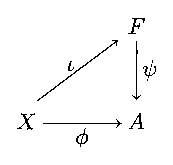
\includegraphics{chap09-vend-scan-01.eps}
\end{figure}

\noindent We observe that $\tilde{M}$ has $c^{\prime}\neq 0$ except possibly when $j=k$. For $c^{\prime}=0$ implies $\tilde{M}(\infty)=\infty$, which amounts to $Mp_{k}=p_{j}$. Since the $p_{i}$ are inequivalent, this forces $j=k$.

Consider the system
\begin{equation*}
\mathbf{T}=\{\tilde{M} \in A_{j}\Gamma A_{k}^{-1}\}|k\ \mathrm{fixed},\ j=1,\,\cdots,\, s;\quad c^{\prime}\neq 0\}.
\end{equation*}

$\mathbf{T}$ is not a group unless $j=k$. With each $\tilde{M} \in \mathbf{T}$ we associate the circle
\begin{equation}
\label{ch09:eqn11}K(\tilde{M}):\bigg|\tau-\bigg(-\frac{d^{\prime}}{c^{\prime}}+\frac{i}{2c^{\prime 2}h}\bigg)\bigg|=\frac{1}{2c^{\prime 2}h},
\end{equation}
where
\begin{equation}
\label{ch09:eqn12} h= \max_{1\leq i,j\leq s}1/\tilde{c}_{ij}>0.
\end{equation}
$(\tilde{c}_{ij}$ is defined in~\ref{ch08:chap08}.~(\ref{ch08:eqn8a})) Observe that $K(\tilde{M})$ is the image by $\tilde{M}^{-1}$ of the horizontal line
\begin{equation*}
\mathscr{E}_{h}=\mathscr{E}(h):y=h.
\end{equation*}
Set
\begin{equation*}
\tag{11a} \mathscr{K} =\{K(\tilde{M})|\tilde{M} \in \mathbf{T}\}.
\end{equation*}


\begin{lemma*}
Two distinct circles of $\mathscr{K}$ do not intersect.
\end{lemma*}

Let $K_{i}=K(\tilde{M}_{i}),\,i=1,\,2$, be two intersecting (not merely tangent) circles of $\mathscr{K}$. Suppose $\tilde{M}_{1}=A_{j_{1}}M_{1}A_{k}^{-1},\,\tilde{M}_{2}=A_{j_{2}}M_{2}A_{k}^{-1}$. Apply $\tilde{M}_{1}$; $K_{1}$ is mapped on $\mathscr{E}_{h}$, while $K_{2}$ is mapped on a circle or straight line
\begin{equation*}
K^{\ast}=A_{j_{1}}M_{1}A_{k}^{-1}A_{k}M_{2}^{-1}A_{j_{2}}^{-1}\mathscr{E}_{h}=A_{j_{1}}MA_{j_{2}}^{-1}\mathscr{E}_{h}.
\end{equation*}
However, if $K^{\ast}$ is a straight line, it must be horizontal since it has to lie in $\mathscr{H}$. But $K_{1}$ cuts $K_{2}$; hence $\mathscr{E}_{h}$ coincides with $K^{\ast}$. This shows that $K_{1}$ is identical with $K_{2}$, against the hypothesis.

We may therefore assume $K^{\ast}$ is a circle. But our choice of $h$ in \eqref{ch09:eqn12} implies that $K^{\ast}$ does not cut $\mathscr{E}_{h}$, for $h\geqq 1/c_{j_{1}j_{2}}^{2}h\geqq 1/c^{\prime 2}h$, the diameter of $K^{\ast}$. This is a contradiction to the hypothesis that $K_{1}$ cuts $K_{2}$.\:\:\:q.e.d.

Let $N>0$. Define
\begin{gather}
\label{ch09:eqn13} \mathbf{T}_{N}^{\prime}=\{\tilde{M} \in \mathbf{T}|0<c^{\prime}<Nh^{-1/2},\,-\lambda_{k}\leqq-d^{\prime}/c^{\prime}<0,\,k\ \mathrm{fixed}\},\\
\label{ch09:eqn14} \mathscr{K}_{N}=\{K(\tilde{M}) |\tilde{M} \in \mathbf{T}_{N}^{\prime}\}.
\end{gather}
Since $\mathscr{K}_{N}$ is a subset of $\mathscr{K}$, it is clear from the lemma that $\mathscr{K}_{N}$ is also a disjoint family. Moreover $\mathscr{K}_{N}$ \emph{is a finite set for each} $N$. Indeed, according to~\ref{ch08:chap08}.~\ref{ch08:sec2D}, there are only a finite number of $c^{\prime}$ in the range $0<c^{\prime}<Nh^{-1/2}$ and, for each $c^{\prime}$, only finitely many $d^{\prime}$ in $0<d^{\prime}\leqq
c^{\prime}\lambda_{k}$. Since $K(\tilde{M})$ depends only on the lower row of $\tilde{M}$, our assertion is valid.

\subsection{}\label{ch09:sec2E} The horizontal line $\mathscr{E}(N^{-2})$ cuts each circle $K$ of $\mathscr{K}_{N}$, for the diameter of $K$ is $1/c^{\prime 2}h$ and by \eqref{ch09:eqn12} this is greater than $N^{-2}$. Since there are only a finite number of circles there is a point of intersection $\bar{\tau}=\overline{x}+iN^{-2}$ farthest to the left. We now choose for the path $L$ (cf. \eqref{ch09:eqn10}) the segment
\begin{equation}
\label{ch09:eqn15} \mathbf{k}(N)=\mathbf{k}=\{\tau|\overline{x}\leqq x<\overline{x}+\lambda_{k},\quad
y=N^{-2}\}.
\end{equation}


\begin{lemma*}
A circle $K(\tilde{M})\in \mathscr{K}$ cuts $\mathbf{k}$ if and only if $K\in \mathscr{K}_{N}$.
\end{lemma*}

There is a first circle $K_{0}=K(\tilde{M}_{0})\in \mathscr{K}_{N}$ that cuts $\mathbf{k}$, namely, the circle that passes through $\bar{\tau}$, and a last circle $K_{1}=K(\tilde{M}_{1})$ that cuts $\mathbf{k}$. There is also a circle $K_{2}\in \mathscr{K}$ that cuts $\mathscr{E}(N^{-2})$ at $\bar{\tau}+\lambda_{k}$. In fact $K_{2}=K(\tilde{M}_{2})$ with $M_{2}= M_{0}P_{k}^{-1}$, for
\begin{equation*}
K(\tilde{M}_{2})=\tilde{M}_{2}^{-1}\mathscr{E}_{h}=A{}_{k}P_{k}M_{0}^{-1}A_{j}^{-1}\mathscr{E}_{h} =U^{\lambda_{k}} \tilde{M}_{0}^{-1}\mathscr{E}_{h}=U^{\lambda_{k}}K_{0}.
\end{equation*}
Suppose $K=K(\tilde{M}) \in \mathscr{K}$ cuts $\mathbf{k},\,\tilde{M} =(\cdot\cdot|c^{\prime}d^{\prime})$. It is immediate that $0<c^{\prime}<Nh^{-1\backslash 2}$. If $-d^{\prime}/c^{\prime}$, the point of tangency of $K$, satisfies $-\lambda_{k}\leqq -d^{\prime}/c^{\prime}<0$, then $K\in \mathscr{K}_{N}$, as desired. If $-d^{\prime}/c^{\prime}\geqq q_{0}$, then $U^{-\lambda_{k}}K$ is, as the equation above shows, an element of $\mathscr{K}$ and in fact of $\mathscr{K}_{N}$, for its point of tangency is to the right of $-\lambda_{k}$. Clearly $U^{-\lambda_{k}}K$ outs $\mathbf{k}$. Since $K$ is to the left of $K_{2}=U^{\lambda_{k}}K_{0},\,U^{-\lambda_{k}}K$ is to the left of $K_{0}$. Then $K_{0}$ is not the first circle of $\mathscr{K}_{N}$ cutting $\mathbf{k}$, a contradiction. Thus assume $-d^{\prime}/c^{\prime}<-\lambda_{k}$. Clearly $K$ lies to the left of $K_{0}$, which is tangent at a point to the right of $-\lambda_{k}$. But then $K$ cannot cut $\mathbf{k}$, again a contradiction.

Conversely, $K\in \mathscr{K}_{N}$ implies $\tilde{M} =(\cdot \cdot |c^{\prime}d^{\prime})\in \mathbf{T}_{N}^{\prime}$. Write $M_{0}= (\cdot \cdot |c^{\prime}_{0}d^{\prime}_{0}),\, M_{1}=(\cdot \cdot |c_{1}^{\prime}d_{1}^{\prime})$. The point of tangency, $-d^{\prime}/c^{\prime}$ of $K$ cannot lie to the left of $-d_{0}^{\prime}/c^{\prime}_{0}$ for this would imply $K$ lies to the left of $K_{0}$, but $K_{0}$ was the first circle in $\mathscr{K}_{N}$ cut by $\mathbf{k}$. Hence $-d^{\prime}/c^{\prime}\geqq-d_{0}^{\prime}/c_{0}^{\prime}$. By the same token $-d^{\prime}/c^{\prime}\leqq-d_{1}^{\prime}/c_{1}^{\prime}$. Thus $K$, if it is not $K_{0}$ or $K_{1}$, lies between them and so cuts $\mathbf{k}$.\:\:\:q.e.d.

Notice that
\begin{equation}
\label{ch09:eqn16} K(\tilde{M}) =K(\tilde{M}_{1})\quad \mathrm{if}\ M_{1}=P_{j}^{m}M,\qquad
m= \mathrm{integer}.
\end{equation}
For
\begin{equation*}
\tilde{M}_{1}=U^{m\lambda_{j}}\tilde{M}=\left(\begin{matrix}
a^{\prime}+m\lambda_{j}c^{\prime} & \cdot\\c^{\prime} & d^{\prime}
\end{matrix}\right),
\end{equation*}
and so
\begin{equation*}
K(\tilde{M}_{1})=\tilde{M}_{1}^{-1}\mathscr{E}_{h}=\tilde{M}^{-1}U^{-m\lambda_{j}}\mathscr{E}_{h}=\tilde{M} ^{-1}\mathscr{E}_{h}=K(\tilde{M}).
\end{equation*}
We select one $\tilde{M}$ in each class $\{U^{m\lambda_{j}}\tilde{M}\}$ by imposing a restriction on $a$: define
\begin{equation}
\label{ch09:eqn17} \mathbf{T}_{N}=\{\tilde{M}\,\in \mathbf{T}|0<c^{\prime}<Nh^{-1/2},\quad
0<d^{\prime}\leqq c^{\prime}\lambda_{k},\quad -c^{\prime}\lambda_{j}\leqq a^{\prime}<0\}.
\end{equation}
Then $\mathbf{T}_{N}$ and $\mathscr{K}_{N}$ are in one-one correspondence. \emph{Hence} $\mathbf{T}_{N}$ \emph{is a finite set}.

\subsection{}\label{ch09:sec2F} The segment $\mathbf{k}$ is partitioned into intervals by the circles of $\mathscr{K}_{N}$. Let
\begin{equation*}
I(\tilde{M}) = \mathrm{Int}\ K(\tilde{M}) \cap \mathbf{k}
\end{equation*}
and
\begin{equation*}
\mathbf{j}=\bigcup\{I(\tilde{M})|\tilde{M}\in \mathbf{T}_{N}\}.
\end{equation*}
This is a partition of $\mathbf{j}$ into disjoint intervals. But $\mathbf{j}$ is not equal to $\mathbf{k}$ and we shall need a partition of
\begin{equation*}
\mathbf{h}=\mathbf{k}-\mathbf{j},
\end{equation*}
The set $\mathbf{h}$ is clearly a union of intervals.

Consider the disks
\begin{equation*}
D_{j}=A_{j}^{-1}(\mathscr{F}_{h}),\quad j=1,\,2,\,\cdots,\,s;\quad \mathscr{F}_{h}=\{\tau|y>h\}.
\end{equation*}
$D_{j}$ has diameter $h^{-1}$ and is tangent to the real axis at $p_{j}$. Write
\begin{equation*}
E=\mathrm{Cl}\ \tilde{R}-\bigcup_{j= 1}^{R}D_{j}.
\end{equation*}

Let $\tau\in \mathbf{h}$. Since $\tilde{R}$ is a fundamental region, there is an $M \in\Gamma$ that sends $A_{k}^{-1}\tau$ into $\mathrm{Cl}\,\tilde{R}$. We claim that $MA_{k}^{-1}\tau$ is, in fact, in $E$. Otherwise it is in some $D_{j}$. Then $\tau^{\prime}=A_{j}MA_{k}^{-1}\tau =\tilde{M}_{\tau}$ lies in $A_{j}(D_{j})=\mathscr{F}_{h}$, so that $\tau\in \tilde{M}^{-1}\mathscr{F}_{h}$. There are now two cases to consider.

First, suppose $\tilde{M}$ does not fix $\infty$. Then $\tilde{M}^{-1}\mathscr{E}_{h}=K(\tilde{M})$ is a circle that cuts $\mathscr{E}(N^{-2})$ since it contains $\tau$ in its interior. Since $\tau\in \mathbf{k},\,K(\tilde{M})$ either cuts $\mathbf{k}$ or $\mathbf{k}$ is completely interior to $K$. The latter possibility can be excluded since it would involve the intersection of $K$ with circles in $\mathscr{K}_{N}$. Therefore $K(\tilde{M})$ cuts $\mathbf{k}$ and from Lemma~\ref{ch09:sec2E} we can conclude that $K(\tilde{M}) \in \mathscr{K}_{N}$. Then $\tau\in I(\tilde{M})$, a contradiction.

Secondly, we must suppose that $\tilde{M}$ fixes $\infty$, which implies $j=k$, since $p_{j}$ and $p_{k}$ are inequivalent when $j\neq k$. Then $M =P_{k}^{m}$ and $\tau^{\prime}= A_{k}MA_{k}^{-1}\tau =U^{m\lambda_{k}}\tau$ is a translation. It is seen that $\tau^{\prime}$ cannot lie in $\mathscr{F}_{h}$, as it is required to do, if
\begin{equation*}
N^{-2}<h,
\end{equation*}
a condition on $N$ we now impose.

We have therefore proved that for each $\tau \in \mathbf{h}$ there is an $M\in\Gamma$ such that $MA_{k}^{-1}\tau\in E$. Define
\begin{gather*}
I(\overline{M})=A_{k}M^{-1}(E)\cap\ \mathrm{h},\qquad \overline{M}=MA_{k}^{-1},\\
\mathbf{T}_{N}^{0}=\{\overline{M}|I(\overline{M})\neq 0\}.
\end{gather*}
Since $E$ is bounded by finitely many arcs of circles, $I (\overline{M})$ is a finite union of intervals and therefore measurable. It is readily seen that the sets $I(\overline{M})$ have disjoint interiors; $\mathbf{T}_{N}^{0}$ is finite for each $N$. Cf. Note 31, p. 408.

Moreover it is trivial that $I(\tilde{M}),\, \tilde{M} \in \mathbf{T}_{N}$, is disjoint from $ I (\overline{M}),\,\overline{M}\in \mathbf{T}_{N}^{0}$. We have now completed our partition of $\mathbf{k}$.


\begin{theorem*}
\begin{gather*}
\mathbf{k}=\mathbf{j}\bigcup \mathbf{h},\\
\mathbf{j}=\bigcup\,\{I(\tilde{M})|\tilde{M}\in \mathbf{T}_{N}\},\qquad \mathbf{h}=\bigcup\{I(\overline{M})|\overline{M}\in \mathbf{T}_{N}^{0}\}
\end{gather*}
is a partition of $\mathbf{k}$ into mutually disjoint measurable sets.
\end{theorem*}

As a consequence of the disjointness we have:
\setcounter{equation}{18}
\begin{equation}
\label{ch09:eqn19} \sum\limits_{\bar{M}}|I(\tilde{M})|+\sum\limits_{\bar{M}}|I(\overline{M})|=\lambda_{k},
\end{equation}
$|I|$ denoting the measure of $I$.

For future reference we remark further:
\begin{gather}
\label{ch09:eqn20} E\ \mathit{is\ a\ compact\ subset\ of}\ \mathscr{H}\ \mathit{contained\ in\ a\ horizontal\ strip}\\
0<h_{0}\leqq y\leqq h_{1}<\infty.\nonumber
\end{gather}
To verify the compactness recall that $\tilde{R}$ is bounded by a finite number of circular arcs.

\subsection{}\label{ch09:sec2G} We are now going to use the above partition of $\mathbf{k}$ to evaluate the integral \eqref{ch09:eqn10} of~\ref{ch09:sec2C}. From \eqref{ch09:eqn10} and Theorem 2F we have
\begin{align*}
\lambda_{k}a_{m}^{(k)}=&\sum\limits_{\tilde{M}\epsilon \mathbf{T}}\int_{I(\tilde{M})}f_{k}(e(w/\lambda_{k}))e(-mw/\lambda_{k}) dw\\
&+\sum\limits_{\overline{M}\epsilon\mathbf{T}^{0}}\int_{I(\overline{M})}f_{k}(e(w/\lambda_{k})) e(-mw/\lambda_{k})dw=S_{1}+S_{2},
\end{align*}
where we have suppressed the parameter $N$ in $\mathbf{T}$ and $\mathbf{T}^{0}$, a practice we shall continue. The term $S_{2}$ is negligible, as we now show.

In each integral of $S_{2}$ apply the transformation equation \eqref{ch09:eqn9} and get
\begin{align*}
S_{2}=&\sum\limits_{\overline{M}\in\mathbf{T}^{0}}\eta(M)\overline{v}(M)\int_{I(\overline{M})}(c^{\prime\prime}w+d^{\prime\prime})^{-r}\\
&\times e(\kappa_{0}w^{\prime\prime}/\lambda_{0}-(m+\kappa_{k}) w/\bar{\lambda}_{k}) f_{0}(e(w^{\prime\prime}/\lambda_{0})) dw
\end{align*}

with $w^{\prime\prime}=MA_{k}^{-1}w$. When $w\in I(\overline{M}),\,w^{\prime\prime}\in E$ (cf. \ref{ch09:sec2F}); hence, by \eqref{ch09:eqn20},
\begin{equation*}
\mathrm{Im}\ w^{\prime}\geqq h_{0}>0.
\end{equation*}
Also $E$ is compact in $\mathscr{H}$; it is therefore mapped by $w^{\prime\prime}\rightarrow e(w^{\prime\prime}/\lambda)$ into a subset of the unit disk where $f$ is free of singularities. It follows that
\begin{equation*}
|f(e(w^{\prime\prime}/\lambda))|\leqq C,
\end{equation*}
$C$ denoting here and from now on a general positive constant that is independent of $m$ and $N$ but may depend on any of the other parameters. Moreover,
\begin{equation*}
|c^{\prime\prime}w+d^{\prime\prime}|^{2}=\mathrm{Im}\ w/\mathrm{Im}\ w^{\prime\prime}\leqq N^{-2}h_{0}^{-1},
\end{equation*}
for $\mathbf{k}$ is at height $N^{-2}$ above the real axis.

Using these results we find
\begin{equation*}
|S_{2}|\leqq\sum\limits_{\overline{M}\in\ \mathbf{T}^{0}}|I(\overline{M})|CN^{r}\exp(C|m|N^{-2})
\end{equation*}
and applying \eqref{ch09:eqn19},
\begin{equation*}
|S_{2}|\leqq CN^{r}\exp(C|m|N^{-2}).
\end{equation*}
In making this estimate we have used the fact that $\kappa_{0}/\lambda_{0}>0$.

This error term will appear repeatedly; we name it
\begin{equation*}
E(m,\,N)=O(N^{r}\exp(C|m|N^{-2})),
\end{equation*}
and so have
\begin{equation*}
S_{2}=E(m,\, N).
\end{equation*}


\subsection{}\label{ch09:sec2H} We now treat $S_{1}$. In each integral of $S_{1}$ apply the transformation formula \eqref{ch09:eqn8} and get
\begin{align*}
S_{1}=&\sum\limits_{\tilde{M}\in \mathbf{T}}\overline{v}(M)\int_{I(\tilde{M})}(c^{\prime}w+d^{\prime})^{-r}\\
&\times e(\kappa_{j} w^{\prime}/\lambda_{j}-(m+\kappa_{k}) w/\lambda_{k}) f_{j}(e(w^{\prime}/\lambda_{j}))dw,
\end{align*}
with $w^{\prime}=\tilde{M}_{w}$. We must be sure the conditions of Theorem 2B are satisfied, that is, that $b^{\prime}<0,\, d^{\prime}>0$ in each $\tilde{M} \in \mathbf{T}$. From the definition \eqref{ch09:eqn17} of $\mathbf{T}=\mathbf{T}_{N}$ we have $d^{\prime}>0,\,c^{\prime}>0,\,a^{\prime}<0$. Now $a^{\prime}d^{\prime}-b^{\prime}c^{\prime}=1$, so $b^{\prime}<0$.

In the above expression for $S_{1}$ replace $f_{j}$ by its expansion \eqref{ch09:eqn3} and separate the principal part, remembering that $w=A_{k}\tau$. The result is
\begin{align*}
S_{1}&=\sum\limits_{\tilde{M}\in \mathbf{T}}\overline{v}(M)\sum\limits_{n=-\mu_{j}}^{-1}a^{(j)}_{n}\int\nolimits_{I(\tilde{M})}(c^{\prime}w+d^{\prime})^{-r}\\
&\qquad\qquad\qquad \times e((n+\kappa_{j}) w^{\prime}/\lambda_{j}-(m+\kappa_{k}) w/\lambda_{k}) dw\\
&\quad +\sum\limits_{\tilde{M}\in \mathbf{T}}\overline{v}(M)\int_{I(\tilde{M})}(c^{\prime}w+d^{\prime})^{-r}\\
&\quad \times\sum\limits_{n =0}^{\infty}a_{n}^{(j)}e((n+\kappa_{j}) w^{\prime}/\lambda_{j}-(m+\kappa_{k}) w/\lambda_{k})dw\\
&=S_{11}+S_{12}.
\end{align*}
In $S_{11}$ we interchanged the order in the finite sum (cf. end of~\ref{ch09:sec2E}) and integral.

The main contribution will, of course, come from $S_{11}$. We first estimate $S_{12}$.

Recall that $\tilde{M}$ maps the interior of $K(\tilde{M})$ on the half-plane $y>h$. Since $I(\tilde{M})$ is interior to $K$, it follows that
\begin{equation*}
\mathrm{Im}\ w^{\prime}\geqq h>0.
\end{equation*}
Moreover,
\begin{equation*}
|c^{\prime}w+d^{\prime}|^{2}=\mathrm{Im}\ w/\mathrm{Im}\ w^{\prime}\leqq N^{-2}h^{-1}.
\end{equation*}
With these estimates we can bound $|S_{12}|$ by
\begin{equation*}
\sum\limits_{\tilde{M}\in \mathbf{T}}|I(\tilde{M})|CN^{r}\exp(C|m|N^{-2})\sum\limits_{n=0}^{\infty}|a_{n}^{(j)}|\exp(-Chn).
\end{equation*}
Since $h>0$ the infinite series converges, for $\exp (-Ch)<1$. The sum of the series is a constant independent of $m$ and $N$. Applying \eqref{ch09:eqn19} we get
\begin{equation*}
S_{12}=E(m,\, N).
\end{equation*}

These results yield
\begin{equation}
\label{ch09:eqn21} \lambda_{k}a_{m}^{(k)}=S_{11}+E(m,\,N).
\end{equation}


\subsection{}\label{ch09:sec2I} The interval $I(\tilde{M})$ divides the circle $K(\tilde{M})$ into two arcs $K^{+}(\tilde{M})$ and $K^{-}(\tilde{M})$, the second being the arc tangent to the real axis. In each integral of $S_{11}$ we now replace the path $1(\tilde{M})$ by $K^{+}(\tilde{M})$, which is permissible by Cauchy's theorem. We have
\begin{equation*}
\tag{$^{\ast}$} \int_{I}=-\int_{K^{+}}=-\int_{K}+\int_{K^{-}},
\end{equation*}
the change in sign resulting from the fact that the integration over the arcs is in the positive sense. For $w$ on $K^{-}$ we have
\begin{equation*}
\mathrm{Im}\ w^{\prime}=h,\qquad |c^{\prime}w+d^{\prime}|^{2}=v/h,\qquad
w=u+iv.
\end{equation*}
Hence
\begin{align*}
\tag{$^{\ast\ast}$} \bigg|\int_{K^{-}}\bigg|\leqq|K^{-}|CN^{r}\exp(2\pi\mu_{j}h/\lambda_{j}+C|m|N^{-2}&)\\
&\leqq|K^{-}|CN^{r}\exp(C|m|N^{-2}).
\end{align*}
Divide $\mathbf{T} =\mathbf{T}_{N}$ into two parts:
\begin{equation*}
\mathbf{T}=\mathbf{T}^{(1)}\cup \mathbf{T}^{(2)},\qquad \mathbf{T}^{(1)}=\bigg\{\tilde{M}=\bigg(\begin{matrix}\cdot
& \cdot\\c^{\prime} & \cdot\end{matrix}\bigg)|0<c^{\prime}<2^{-1}h^{-1/2}N\bigg\}.
\end{equation*}
Now $K(\tilde{M})$ is a circle of diameter $1/c^{\prime2}h$ and $K^{-}(\tilde{M})$ is an arc that subtends the chord $\mathbf{k}$ at height $N^{-2}$. Since in $\mathbf{T}^{1}$ we have $N^{-2}<2^{-1}c^{\prime-2}h^{-1}$, in other words, the subtended chord lies below the horizontal diameter of $K$, it follows that the ratio of arc to chord length is bounded above by an absolute constant. That is, $|K^{-}|/|I|<\pi/2$, and so
\begin{equation*}
\sum\limits_{\mathbf{T}^{(1)}}|K^{-}(\tilde{M})<C\sum|I(\tilde{M})|\leqq C\lambda_{k}=C.
\end{equation*}

Now consider the circles $K(\tilde{M})$ in $\mathbf{T}^{(2)}$. Since here $2^{-1}h^{-1/2}N\leqq c^{\prime}<h^{-1/2}N$, the diameter of the largest circle is not more than $4/N^{2}$. Each circle is tangent to the real axis at a point on the interval $(0,\,\lambda_{k})$; hence all circles lie in a region of area less than $4N^{-2}(\lambda+4N^{-2})\leqq CN^{-2}$. But the circles do not overlap (Lemma \ref{ch09:sec2D}). If $\Lambda$ is the number of circles, then $CN^{-2}>\Lambda\cdot\pi 4^{-1}N^{-4}$, for the diameter of a circle is always more than $N^{-2}$ since it must intersect $\mathbf{k}$. The sum of the circumferences of all circles is, however, less than $4\pi N^{-2}\Lambda$, and this is now less than $C$. \emph{A fortiori}
\begin{equation*}
\sum\limits_{T^{(2)}}|K^{-}(\tilde{M})|<C.
\end{equation*}

We use these results in $(\ast\ast)$ to obtain
\begin{equation*}
\bigg|\sum\limits_{M\in \mathbf{T}}\int_{K^{-}(\tilde{M})}\cdots dw\bigg|=E(m,\,N),
\end{equation*}
and from \eqref{ch09:eqn21} and $(^{\ast})$,
\begin{align*}
\lambda_{k} a_{m}^{(k)}= &-\sum\limits_{\tilde{M}\in \mathbf{T}}\overline{v}(M)\sum\limits_{\nu= 1}^{\mu_{j}}a_{-\nu}^{(j)}\int\nolimits_{K(\tilde{M})}(c^{\prime}w+d^{\prime})^{-r}\\
&\times e(-\nu_{j}w^{\prime}-m_{k}w)dw\,+E(m,\,N),
\end{align*}
where we have replaced $n$ by $-\nu$ and have set
\begin{equation*}
m_{k}=(m+\kappa_{k})/\lambda_{k},\qquad \nu_{j}=(\nu-\kappa_{j})/\lambda_{j}.
\end{equation*}


\subsection{}\label{ch09:sec2J} The purpose of replacing the integral over $I(\tilde{M})$ by one over $K(\tilde{M})$ was, of course, to obtain an integral over a closed curve, to which the theorem of residues can be applied. In this case, however, it is more convenient to bring the integral into a known form by means of a substitution. Let $w+d^{\prime}/c^{\prime}=i/p$; then
\begin{equation*}
w^{\prime}=a^{\prime}/c^{\prime}-1/c^{\prime 2}(w+d^{\prime}/c^{\prime})=a^{\prime}/c^{\prime}-p/ic^{\prime
2}.
\end{equation*}
Thus
\begin{equation*}
\int_{K(\tilde{M})}=i(ic^{\prime})^{-r}e((m_{k} d^{\prime}-\nu_{j}a^{\prime})/c^{\prime})\int_{\alpha-i\infty}^{\alpha+i\infty}p^{r-2}\exp\{2\pi(p\nu_{j}c^{\prime
-2}+m_{k}p^{-1})\}dp
\end{equation*}
with $\alpha=c^{\prime 2}h>0$. Recall that $r\leqq 0$. The integral is an inverse Laplace transform whose value may be found in H. \citeauthor{Bateman0000}~[\ref{Bateman1}, p. 245]\index{Bateman, H.}. Define
\begin{equation}\label{ch09:eqn22}
L(c,\, \sigma,\,\rho,\,r)=\begin{cases}
(\rho/\sigma)^{(r+1)/2}I_{r+1}(4\pi\sigma^{1/2}\rho^{1/2}/c),\qquad \sigma>0\\
(2\pi\rho/c)^{r+1}/\Gamma(r+2),\qquad \sigma=0,
\end{cases}
\end{equation}
where $I_{r+1}$ is the Bessel function given by the power series
\begin{equation*}
\tag{22a}I_{r+1}(z\displaystyle )=\sum\limits_{l=0}^{\infty}\frac{(z/2)^{r+1+2l}}{l!\Gamma(r+l+2)}.
\end{equation*}
We then have
\begin{equation*}
\int_{\alpha-i\infty}^{\alpha+i\infty}=2\pi ic^{\prime r-1}L(c^{\prime},\,m_{k},\,\nu_{j},\,-r).
\end{equation*}
Inserting this result we get
\begin{align}
\label{ch09:eqn23} \lambda_{k}a_{m}^{(k)}=&2\pi i^{-r}\sum\limits_{\bar{M}\in\mathbf{T}_{N}}\overline{v}(M)e((m_{k}d^{\prime}-\nu_{j}a^{\prime})/c^{\prime})\sum\limits_{\nu=1}^{\mu_{j}}a_{-\nu}^{(j)}\\ &\times c^{\prime-1}L(c^{\prime},\,m_{k},\,\nu_{j},\,-r)+E(m,\,N).\nonumber
\end{align}

We now consider the case $r<0$. Keep $m$ fixed and let $N\rightarrow\infty$. Then $E(m,\,N)\rightarrow 0$. The finite sum becomes an infinite series which converges, since the left member is independent of $N$. This is essentially the final result.


\subsection{}\label{ch09:eqn2K} We can simplify the right member of \eqref{ch09:eqn23} to a certain extent. The matrices $\tilde{M}$ of $\mathbf{T}_{N}$ are determined by their second row, for it is easy to check that when $c^{\prime},\,d^{\prime}$ are given there is only one matrix $\tilde{M}$ with $a^{\prime}$ in the range $-c^{\prime}\lambda_{j}\leqq a^{\prime}<0$. Hence the summation over $\mathbf{T}_{N}$ may be written
\begin{equation*}
\sum\limits_{j= 1}^{s}\sum\limits_{c^{\prime}}\sum\limits_{d^{\prime}},
\end{equation*}
where $c^{\prime}\in C_{jk},\,0<c^{\prime}<h^{-1/2}N$, and $d^{\prime}\in D_{c^{\prime}}(j,\, k;-\infty,\,\infty),\,0<d^{\prime}\leqq c^{\prime}\lambda_{k}$. (Cf.~\ref{ch08:chap08}. \ref{ch08:sec2D}.) Furthermore, the range of $d^{\prime}$ may be replaced by any half-open interval of length $\lambda_{k}$. In fact, this means merely that a certain interval in the range of $d^{\prime}$ is replaced by a translate: $d^{\prime}\rightarrow d^{\prime}+nc^{\prime}\lambda_{k}$. But the terms in the right member of \eqref{ch09:eqn23} are invariant under this replacement. The exponential term picks up the factor $e(\kappa_{k}n)$. But with $\tilde{M}_{1}= (\cdot \cdot|c^{\prime},\,d^{\prime}+nc^{\prime}\lambda_{k})=\tilde{M}U^{n\lambda_{k}}$, i.e., $M_{1}=MP_{k}^{n}$, we have (\ref{ch08:chap08}.~\ref{ch09:sec2E})
\begin{equation*}
v(M_{1})=v(MP_{k}^{n})=v(M)v(P_{k}^{n})=v(M) e(\kappa_{k}n),
\end{equation*}
which proves our statement. Hence we may replace the above range of $d^{\prime}$ by: $0 \leqq d^{\prime}<c^{\prime}\lambda_{k}$.

Our sum can now be written
\begin{equation*}
\sum\limits_{j=1}^{s} \sum\limits_{\substack{c^{\prime}\in C_{jk}\\0<c^{\prime}<h^{-1/2}N}}\sum\limits_{d^{\prime}\in D_{c^{\prime}}}
\end{equation*}
where, as an abbreviation, we have written $D_{c^{\prime}}$ for $D_{c^{\prime}}(j,\, k;\,0,\, c^{\prime}\lambda_{k})$. The summation over $d^{\prime}$ can be carried out by defining
\begin{equation}
\label{ch09:eqn24} A(c^{\prime},\,m_{k},\,\nu_{j})=\sum\limits_{d^{\prime}\in D_{c^{\prime}}}\overline{v}(M)e((m_{k}d^{\prime}-\nu_{j}a^{\prime})/c^{\prime}).
\end{equation}
We can now let $N\rightarrow\infty$ and obtain the final formula:
\begin{align}
\label{ch09:eqn25} \lambda_{k}a_{m}^{(k)}=2\pi i^{-r}\sum^{s}_{j=1}\sum^{\mu_{j}}_{\nu=1}a_{-\nu}^{(j)}\sum\limits_{\substack{c^{\prime}\in
C_{jk}\\c^{\prime} >0}}c^{\prime -1}A(c^{\prime},\,m_{k},\,\nu_{j}) L(c^{\prime},\,m_{k},\,&\nu_{j},-r),\\
&k=1,\,2,\cdots\,s.\nonumber
\end{align}


\subsection{}\label{ch09:sec2L} In case $r=0$ the error term $E(m,\,N)$ does not tend to $0$ with increasing $N$ ($m$ fixed). The best we can do is to couple the variation\index{automorphic forms of zero dimension!expansion coefficients of} of $m$ and $N$ in such a way that $E$ remains bounded. For this purpose set
\begin{equation*}
N=\sqrt{mh}
\end{equation*}
and then get
\begin{equation}
\label{ch09:eqn26}\lambda_{k}a_{m}^{(k)}=2\pi\sum\limits_{j= 1}^{s}\sum\limits_{\nu= 1}^{\mu}a_{-\nu}^{(j)},\sum\limits_{c^{\prime}\in C_{jk};0<c^{\prime}<\sqrt{}m}c^{\prime-1}A(c^{\prime},\,m_{k},\,\nu_{j})L(c^{\prime},\,m_{k},\,\nu_{j},\,0)+E_{m},
\end{equation}
where $E_{m}=E(m, \sqrt{mh})$ is bounded in $m\geqq 1$.

Our results are contained in the following


\begin{theorem*}
Let $F(\tau)\in\{\Gamma,\,-r,\,v\}$. The coefficients\index{automorphic forms of positive dimension!expansion coefficients of} $a_{m}^{(k)},\,m\geqq 0$, in the expansion \eqref{ch09:eqn3} of $F$ are given by \eqref{ch09:eqn25} when $r<0$ and by \eqref{ch09:eqn26} when $r=0$.
\end{theorem*}

\subsection{}\label{ch09:2M} Nothing in our analysis required $F$ to have poles. If $F$ is everywhere regular (i.e., regular in $\mathscr{H}^{+})$, we have $a_{-\nu}^{(j)}=0,\,j=1,\,2,\,\cdots,\,s,\,\nu=1,\, 2,\, \cdots,\, \mu_{j}$. If now $r<0$, our result shows that $a_{m}^{(k)}=0$ for $m\geqq 0$ ($k$ fixed). Hence $F\equiv 0$.


\begin{theorem*}
The only everywhere regular automorphic form of positive dimension is $0$.
\end{theorem*}

This generalizes Theorem~\ref{ch09:sec1B} so far as forms of positive dimension are concerned since now the dimension need not be an integer.

\subsection{}\label{ch09:sec2N} We are often interested in the Fourier series\index{automorphic forms of positive dimension!Fourier coefficients of}\index{automorphic forms of zero dimension!Fourier coefficients of} (expansion at $i\infty$) of an automorphic form (\ref{ch08:chap08}. (14a)):
\begin{equation*}
e(-\kappa_{0}\tau/\lambda_{0})F(\tau)=f_{0}(t)=\sum\limits_{m=-\mu_{s}}^{\infty}a_{m}^{(0)}e(m\tau/\lambda_{0}).
\end{equation*}
To obtain the Fourier coefficients $a_{m}^{(0)}$ in the simplest form it is advisable to work through the above method again, choosing this time a fundamental region having a cusp at $i\infty$. We renumber the cusps $p_{0}=i\infty,\,p_{1},\ldots,p_{s-1}$. Everything goes through as before, with minor modifications, if we replace $k$ by $0,\,A_{k}$ by $I$. Hence:


\begin{theorem*}
The Fourier coefficients $a_{m}^{(0)},\,m\geqq 0$, \emph{of} $F(\tau)\in\{\Gamma,\, -r,\,v\}$ are given by \eqref{ch09:eqn25} when $r<0$ and by \eqref{ch09:eqn26} when $r =0$ provided we put $k=0$ and sum $j$ over $0,\, 1,\, \cdots,\,s -1$.
\end{theorem*}

\section{Expansions of Zero}\label{ch09:sec3}

After Rademacher\index{Rademacher} obtained his convergent series for the partition function\footnote{Cf.~\ref{ch11:chap11}.~\ref{ch11:sec2A}. This series appears in our development as a special case of Theorem 2N.} $p(n)$, he inserted this series into the generating function\index{expansion of zero}
\begin{equation*}
\varphi(t)=\prod_{m=1}^{\infty}(1-t^{m})^{-1},\qquad |t|<1
\end{equation*}
and rearranged the terms, getting
\begin{equation}
\label{ch09:eqn27} \varphi(t)=1+\sum\limits_{h,k}\alpha_{hk}\Phi_{k}(t\varepsilon_{hk}^{-1}),\qquad
|t|<1.
\end{equation}
Here $h/k$ runs over all reduced fractions in $(0,\,1),\, \alpha_{hk}$ is a constant, $\varepsilon_{hk} =e(h/k)$, and the function $\Phi_{k}(t\varepsilon_{hk}^{-1})$ is regular everywhere except at $t=\varepsilon_{hk}$. The formula \eqref{ch09:eqn27} can be regarded as a generalized partial fraction decomposition of $\varphi(t)$. The natural boundary $(|t|=1)$ is made up of contributions from the ``partial fractions'' $\Phi_{k}$, one for each root of unity $\varepsilon_{hk}$. (\citeauthor{Rademacher0000}~[\ref{Rademacher2}].)

Rademacher noticed that the \emph{series} in \eqref{ch09:eqn27} converges also when $|t|>1$. He defined a function
\begin{equation*}
\varphi^{\ast}(t)=1+\sum\limits_{h,k}\alpha_{hk}\Phi_{k}(t\varepsilon_{hk}^{-1}),\qquad
|t|>1
\end{equation*}
and proved that
\begin{equation*}
\varphi^{\ast}(t)=-\sum\limits_{n= 1}^{\infty}p(-n) t^{-n},\qquad |t|>1
\end{equation*}
where $p(-n)$ is the expression obtained by formally replacing $n$ by $-n$ in the series for $p(n)$. He conjectured ([2]) and later proved ([7]) the surprising fact that
\begin{equation*}
p(-n)=0,\qquad n=1,\,2,\,\cdots.
\end{equation*}
(Cf. also \citeauthor{Petersson0000}~[\ref{Petersson5}]\index{Petersson}.) Thus
\begin{equation}
\label{ch09:eqn28} \varphi^{\ast}(t)\equiv 0,\qquad |t|>1.
\end{equation}
Equation \eqref{ch09:eqn28} is called an ``expansion of zero''.

Since $\varphi,\,\varphi^{\ast}$ are closely related to modular forms, we have in \eqref{ch09:eqn28} a type of behavior similar to that already noticed by Poincar\'{e}\index{Poincar\'{e}} and commented on by us in~\ref{ch05:chap05}.~\ref{ch05:sec2G}.

It is the purpose of this Section to generalize the above discussion to forms of positive dimension on $H$-groups. In order not to complicate the formulas unduly, we shall assume that $\Gamma$ has a single parabolic cusp, which we place at $i\infty$.

\subsection{}\label{ch09:sec3A} Let $F\in\{\Gamma,\,-r,\,v\}$ have the Fourier series
\begin{equation}
\label{ch09:eqn29}F(\displaystyle \tau)=P(\tau)+\sum\limits_{m=0}^{\infty}a_{m}^{(0)}e((m+\kappa_{0})\tau/\lambda_{0}), \end{equation}
where
\begin{equation*}
P(\tau)=\sum\limits_{\nu=1}^{\mu}b_{-\nu}e((-\nu+\kappa_{0})\tau/\lambda_{0}).
\end{equation*}
By Theorem $2N$ the coefficients $a_{m}^{(0)}$ are given by
\begin{equation*}
a_{m}^{(0)}=2\pi i^{-r}\lambda_{0}^{-1}\sum\limits_{\nu= 1}^{\mu}b_{-\nu}\sum\limits_{c\in C^{\prime}}c^{-1}A(c,\, m_{0},\,\nu_{0}) L(c,\, m_{0},\,\nu_{0},\,-r),\qquad
m\geqq 0
\end{equation*}
where we have written
\begin{equation*}
C^{\prime}=\{c\in C_{00},\,c>0\},\qquad m_{0}=\frac{m+\kappa_{0}}{\lambda_{0}},\qquad
\nu_{0}=\frac{\nu-\kappa_{0}}{\lambda_{0}}.
\end{equation*}

We fix our attention on the case $\kappa_{0}>0$. Define
\begin{equation}
\label{ch09:eqn30} L_{c}(m)=L(c, m_{0},\,\nu_{0},\,-r),\qquad \Phi_{c,\nu}(z)=\Phi_{c}(z)=\sum\limits_{m=0}^{\infty}L_{c}(m) z^{m};
\end{equation}
then
\begin{equation}
\begin{split}
&a_{m}^{(0)}=\sum\limits_{\nu=1}^{\mu}b_{-\nu}\sum\limits_{c\in C^{\prime}} \sum\limits_{d\in D_{c}}\alpha_{cd}L_{c}(m)e(md/c\lambda_{0}),\\
&\alpha_{cd}=2\pi i^{-r}\lambda_{0}^{-1}c^{-1}\overline{v}(M) e((\kappa_{0}d-\nu_{0}a)/c\lambda_{0}),\qquad
M=\bigg(\begin{matrix}\cdot & \cdot\\c & d\end{matrix}\bigg).
\end{split}\label{ch09:eqn31}
\end{equation}
Now insert this formula in \eqref{ch09:eqn29}, interchange the order of summation, and obtain
\begin{equation}
\label{ch09:eqn32} F(\tau)=P(\tau)+\sum\limits_{\nu=1}^{\mu}b_{-\nu}\sum\limits_{c,d}\alpha_{cd}e(\kappa_{0}\tau/\lambda_{0})\Phi_{c}(t\varepsilon_{cd}),\qquad |t|<1
\end{equation}
where
\begin{equation*}
t=e(\tau/\lambda_{0}),\qquad \varepsilon_{cd}=e(d/c\lambda_{0}).
\end{equation*}
The order inversion can be legitimatized by the type of estimate employed in~\ref{ch08:chap08}. \ref{ch08:sec7G}.

Let us study this formula. We first want to determine the analytic character of $\Phi_{c}$. Now the power series for $I_{-r+1}$ (cf. (22a)) shows that $L_{c}(m)$ is an entire function of $m$. Moreover
\begin{equation}
\label{ch09:eqn33} L_{c}(m)=O(\exp\, (Cm^{1/2})),\qquad m\rightarrow\infty
\end{equation}
as we can see from the well-known asymptotic formula for the Bessel function (\citeauthor{Whittaker0000}\index{Whittaker-Watson} [\ref{Whittaker}, p. 373]),
\begin{equation*}
I_{-r+1}(z)\sim e^{z}(2\pi z)^{-1/2}.
\end{equation*}
Here $C$ may be chosen to depend only on $\mu$.

Let the Taylor series of $L_{c}$ be
\begin{equation*}
L_{c}(t)=\sum\limits_{n= 0}^{\infty}\frac{a_{cn}}{n!}t^{n}.
\end{equation*}
By Cauchy's inequality and \eqref{ch09:eqn33} we derive
\begin{equation*}
|a_{cn}|\leqq n!\frac{|L_{c}(n^{2})|}{(n^{2})^{n}}=O\bigg(\frac{Cn}{n!}\bigg),
\end{equation*}
where again $C$ depends only on $\mu$. Define\footnote{The function $l(s)$ is the Laplace transform of $L_{c}(t)$, but we do not need this fact here. The use of the Laplace transform in this and the next subsection was suggested by Professor Pisot.\index{Pisot}}
\begin{equation*}
\tag{$^{\ast}$} l(s)= \sum\limits_{n=0}^{\infty}\frac{a_{cn}}{s^{n+1}}.
\end{equation*}
From the estimate for $a_{cn}$ it is clear that the series converges, and $l(s)$ is bounded, outside any circle $|s|=\eta>0$.

Next,
\begin{equation*}
\tag{$\dagger$} L_{c}(t)=\displaystyle \frac{1}{2\pi i}\int_{|s|=\eta}e^{s t}l(s) ds,
\end{equation*}
as can be seen by inserting $(^{\ast})$ and integrating term by term.

We now can find a new expression for $\Phi_{c}(z)$. Let $z$ be such that $|ze^{s}|\leqq\rho<1$ for $|s| =\eta$. Then from $(\dagger)$,
\begin{equation}
\begin{split}
\label{ch09:eqn34}\Phi_{c}(z)&=\sum\limits_{n=0}^{\infty}L_{c}(m) z^{m}=\sum\limits_{11}^{\infty}z^{m}\frac{1}{\sim\pi i}\int_{|s|=\eta}e^{sm}l(s) ds\\
&=\frac{1}{2\pi i}\int_{|s|=\eta}\frac{l(s)}{1-ze^{s}}ds.
\end{split}
\end{equation}
Thus the integral agrees with $\Phi_{c}$ for small $z$; it therefore provides the analytic continuation of $\Phi_{c}$ wherever it converges. This is the case if $-\log z$ is outside the circle $|s|=\eta$, i.e., $|\log z|>\eta$. For any $\zeta\neq 1$ we can find $\eta_{1}<\eta$ so that $|\log\zeta|>\eta_{1}$. According to Cauchy's theorem the path may be shrunk to $|s|= \eta_{1}$ and
the new integral represents $\Phi_{c}(z)$ for all $z$ for which $|\log z|>\eta_{1}$,
in particular for $z=\zeta$. Hence: $\Phi_{c}(z)$ \emph{is regular in the whole complex sphere except at} $z=1$. Note in particular that $\Phi_{c}(\infty)=0$.

Formula \eqref{ch09:eqn32} may be regarded as a generalized partial fraction decomposition of $F(\tau)$ considered as a function of $t$ in $|t|<1$, the function\footnote{We recall from \eqref{ch09:eqn30} that $\Phi_{c}$ depends on $\nu$.} $\sum\nolimits_{\nu=1}^{\mu}b_{-\nu}\Phi_{c}(t\varepsilon_{cd})$ contributing the singularity at $t=1/\varepsilon_{cd}$. Since $\Gamma$ is horocyclic, the points $\{-d/c\}$ are dense on the real axis, and this shows that the singularities $\{\varepsilon_{c d}\}$ fill out, in their closure, the entire unit circle.


\subsection{}\label{ch09:sec3B} We are now going to sum the \emph{series} in \eqref{ch09:eqn32} when $|t|>1$. For this purpose we first derive an explicit formula for the continuation of $\Phi_{c}$, to the exterior of the unit circle. In fact, if $|z|>1$, there is an $\eta$ which satisfies not only $|\log z|>\eta$ but also
\begin{equation*}
|ze^{s}|\geqq\sigma>1,\qquad |s|=\eta.
\end{equation*}
Hence \eqref{ch09:eqn34} gives
\begin{align}
\Phi_{c}(z)&=\mathop{\mathrm{Res}}_{s=0}\frac{l(s)}{1-ze^{s}}=-\mathop{\mathrm{Res}}_{s=0}\sum\limits_{n=0}^{\infty}\frac{a_{c n}}{s^{n+1}}\sum\limits_{m=1}^{\infty}(ze^{s})^{-m}\nonumber\\
&=-{\rm Res}\sum\limits_{n=0}^{\infty}\sum\limits_{m=1}^{\infty}a_{cn}z^{-m}\sum\limits_{l=0}^{\infty}\frac{(-sm)^{l}}{l!}s^{-n-1}\nonumber\\
&=\sum\limits_{n=0}^{\infty}\sum\limits_{m=1}^{\infty}a_{cn}z^{-m}\frac{(-m)^{n}}{n!},\nonumber\\
\label{ch09:eqn35}\Phi_{c}(z)&=\sum\limits_{m=1}^{\infty}L_{c}(-m) z^{-m},\qquad |z|>1.
\end{align}
This is the desired continuation formula.


\subsection{}\label{ch09:sec3C} We return to the series \eqref{ch09:eqn32}. Let $F^{\ast}(\tau)$ be the sum of the series when $\mathrm{Im}\ \tau<0$ or $|t|>1$. Using \eqref{ch09:eqn35} we get
\begin{align*}
&F^{\ast}(\tau)-P(\tau)=-\sum\limits_{\nu=1}^{\mu}b_{-\nu}\sum\limits_{c,d}\alpha_{cd}e\bigg(\frac{\kappa_{0}\tau}{\lambda_{0}}\bigg)\sum\limits_{m=1}^{\infty}L_{c}(-m)\cdot(t\varepsilon_{cd})^{-m}\\
=&-\sum\limits_{m=1}^{\infty}e((-m+\kappa_{0})\tau/\lambda_{0})\sum\limits_{\nu=1}^{\mu}b_{-\nu}\sum\limits_{c,d}\alpha_{cd}e(-md/c\lambda_{0})L_{c}(-m).
\end{align*}
We recognize the inner sum as $a_{-m}^{(0)}$, by which we mean the expression obtained by replacing $m$ by $-m$ in the series \eqref{ch09:eqn31} for $a_{m}^{(0)}$. That is,
\begin{equation*}
F^{\ast}(\tau)=P(\tau)-\sum\limits_{m=1}^{\infty}a_{-m}^{(0)}e((-m+\kappa_{0})\tau/\lambda_{0}),\qquad
\mathrm{Im}\ \tau<0.
\end{equation*}


\subsection{}\label{ch09:sec3D} The coefficients of \emph{this} series, however, are mostly zero!\index{expansion of zero}


\begin{theorem*}
Let $a_{m}^{(0)}$ be defined for all integer values of $m$ by \eqref{ch09:eqn31}. Then
\begin{equation}
\begin{split}
&a_{-m}^{(0)}=0,\qquad m>\mu\\
&a_{-m}^{(0)}=b_{-m},\quad m=1,\,2,\,\cdots,\,\mu.
\end{split}\label{ch09:eqn36}
\end{equation}
\end{theorem*}

The following elegant proof of this remarkable result is due to Rademacher.\index{Rademacher} Formula \eqref{ch09:eqn31} holds for all values of $m$, negative integers included, for an examination of the developments of Section~\ref{ch09:sec2} reveals that they depend in no way on the nonnegativity of $m$. The theorem then follows immediately from the Fourier series expansion \eqref{ch09:eqn29} of $F(\tau)$.

We conclude that
\begin{equation}
\label{ch09:eqn39} F^{\ast}(\tau)\equiv 0,\quad \mathrm{Im}\ \tau<0.
\end{equation}
This equation may properly be called an expansion of zero.

\subsection{}\label{ch09:sec3E} Since $F^{\ast}$ is the sum of the same series that defines $F$, we suspect that it may be closely related to an automorphic form.\index{automorphic forms of positive dimension!expansion coefficients of}\index{complementary form!Fourier coefficients of} This is the case, but the form in question is one of \emph{negative} dimension, the so-called \emph{complementary} form.\index{complementary form}


\begin{definition*} Two forms $F,\,G$ are said to be complementary if and only if their product $FG$ belongs to $\{\Gamma,\,-2,1\}$.

Thus $F$ and $G$ are complementary provided $FG$ is a \emph{differential} on the Riemann surface $\Gamma\backslash \mathscr{H}^{+}$. Suppose $F\in\{\Gamma,\,-r,\,v\}$ and has the parameter $\kappa_{0}$. Now $\overline{v}=1/v$ is a multiplier for the dimension $r$, hence for $r-2$. Also, $\overline{v}(U)=e(-\kappa_{0}) =e(1-\kappa_{0})$. It follows that $G \in\{\Gamma,\,r-2,\overline{v}\}$ and has the parameter
\begin{equation}
\label{ch09:eqn38} \kappa_{0}^{\prime}=\begin{cases}
1-\kappa_{0}, & \kappa_{0}>0\\0, & \kappa_{0}=0.
\end{cases}
\end{equation}

To abbreviate the discussion we shall consider only the case in which $F(\tau)$ has a single term in its principal part. That is, we assume there exists a form $F_{\mu}$ with Fourier series
\begin{equation*}
F_{\mu}(\tau)=e((-\mu+\kappa_{0})\tau/\lambda_{0})+ \mathrm{const} + \cdots.
\end{equation*}
\end{definition*}

\begin{theorem*}
Denote the Fourier coefficients of $F_{\mu}(\tau)$ by $a_{m}(\mu,\, -r,\, v)$. Then
\begin{gather*}
c_{m-1}(\mu-1,\,r-2,\,\overline{v})=2e(-r/2)\bigg(\frac{-m+\kappa_{0}}{\mu-\kappa_{0}}\bigg)^{-r+1}\overline{a}_{-m}(\mu,\,-r,\,v),\\
\mu\geqq 1,\qquad m\geqq 1,\qquad \kappa_{0}>0
\end{gather*}
where $c_{m}(\mu,\,-r,\,v)$ is the mth Fourier coefficient \emph{(}at $i\infty$\emph{)} of the Poincar\'{e} series $G_{-r}(\tau,\,\overline{v},\,\Gamma,\,\mu\,+\kappa_{0}^{\prime})$. \emph{(Cf.~\ref{ch08:chap08}.~\eqref{ch08:eqn16}).)}
\end{theorem*}

For the proof we compare the representations~\ref{ch08:chap08}.~\eqref{ch08:eqn42} of $c_{m}$ and \eqref{ch09:eqn25} of $a_{m}$:
\begin{align*}
c_{m-1}(\mu-1,\,r-2,\overline{v})=&-4\pi i^{r}\lambda_{0}^{-1} \sum\limits_{c\in
C^{\prime}}c^{-1}W_{c}(m-1,\,\mu-1+\kappa_{0}^{\prime})\\
&\times M\bigg(c,\frac{m-1+\kappa_{0}^{\prime}}{\lambda_{0}},\frac{\mu-1+\kappa_{0}^{\prime}}{\lambda_{0}},2-r\bigg),
\end{align*}

\begin{align*}
a_{-m}(\mu,\,-r,\,v)=&2\pi i^{-r}\lambda_{0}^{-1}\sum\limits_{c\in C^{\prime}}c^{-1}A\bigg(c,\,\frac{-m+\kappa_{0}}{\lambda_{0}},\frac{\mu-\kappa_{0}}{\lambda_{0}}\bigg)\\
&\times L\bigg(c,\,\frac{-m+\kappa_{0}}{\lambda_{0}},\,\frac{\mu-\kappa_{0}}{\lambda_{0}},\,-r\bigg).
\end{align*}
Now $m-1+\kappa_{0}^{\prime}=m-\kappa_{0},\,\mu -1+\kappa_{0}^{\prime}=\mu-\kappa_{0}$, provided $\kappa_{0}>0$. Also
\begin{align*}
M\bigg(c, \frac{m-\kappa_{0}}{\lambda_{0}},\frac{\mu-\kappa_{0}}{\lambda_{0}},2-r\bigg)=&e\bigg(\frac{1-r}{2}\bigg)\cdot\bigg(\frac{-m+\kappa_{0}}{\mu-\kappa_{0}}\bigg)^{-r+1}\\
&\times L\bigg(c,\,\frac{-m+\kappa_{0}}{\lambda_{0}},\,\frac{\mu-\kappa_{0}}{\lambda_{0}},-r\bigg),
\end{align*}
and
\begin{equation*}
W_{c}(m\,-1,\,\mu-\kappa_{0})=\overline{A}\bigg(c,\,\frac{-m+\kappa_{0}}{\lambda_{0}},\,\frac{\mu-\kappa_{0}}{\lambda_{0}}\bigg),
\end{equation*}
$\overline{A}(\cdots)$ denoting the complex conjugate of $A(\cdots)$. Since $L(\cdots)$ is real for $m,\,\mu \geqq 1$, this gives the desired result.

\subsection{}\label{ch09:sec3F} Utilization of \eqref{ch09:eqn36} completes the proof of the case $\kappa_{0}>0$ of the following


\begin{theorem*}
Let $F_{\mu}(\tau)\in\{\Gamma,\,-r,\,v\},\,r<0$, have the Fourier expansion\index{complementary form!Fourier coefficients of}
\begin{equation*}
F_{\mu}(\tau)=\ e((-\mu+\kappa_{0})\tau/\lambda_{0})+\sum\limits_{m=0}^{\infty}a_{m}(\mu,\,-r,\, v) e((m+\kappa_{0})\tau/\lambda_{0}).
\end{equation*}
Let $G_{r-2}(\tau,\overline{v},\,\mu+\kappa_{0}^{\prime})\in\{\Gamma,\,r-2,\,\overline{v}\}$ have the Fourier expansion
\begin{align*}
G_{r-2}(\tau,\,\overline{v},\, \mu+\kappa_{0}^{\prime})=&\ 2e((\mu+\kappa_{0}^{\prime})\tau/\lambda_{0})+\sum\limits_{m=0}^{\infty}c_{m}(\mu,\, r-2,\overline{v})\\
&\times e((m+\kappa_{0}^{\prime})\tau/\lambda_{0}),
\end{align*}
will $\kappa_{0}^{\prime}$ given by \eqref{ch09:eqn38}. Then for $\kappa_{0}^{\prime}>0$,
\begin{subequations}
\begin{equation}
\begin{split}
&c_{m}(\mu-1,\,r-2,\,\overline{v})=0,\qquad 0<m\neq\mu-1;\\
&\qquad\qquad c_{\mu-1}(\mu-1,\,r-2,\,\overline{v})=-2;
\end{split}\label{ch09:eqn39a}
\end{equation}
while for $\kappa_{0}^{\prime}=0$,
\begin{equation}
\begin{split}
&c_{m}(\mu,\,r-2,\overline{v})=0,\qquad 0<m\neq\mu;\\
&\qquad\qquad c_{\mu}(\mu,\,r-2,\overline{v})=-2.
\end{split}\label{ch09:eqn39b}
\end{equation}
\end{subequations}
Hence
\begin{align*}
G_{r-2}(\tau,\overline{v},\,\mu-1+\kappa_{0}^{\prime})&\equiv 0,\qquad \kappa_{0}^{\prime}>0\\
G_{r-2}(\tau,\,\overline{v},\,\mu)&\equiv 0,\qquad \kappa_{0}^{\prime}=0.
\end{align*}
\end{theorem*}

The proof when $\kappa_{0}=0$ is made by similar arguments and will be omitted. The identities \eqref{ch09:eqn36} and \{(\ref{ch09:eqn39a}), (\ref{ch09:eqn39b})\} are of the same structure.

M. I. Knopp\index{Knopp, M. I.} has established the converse theorem for \emph{integral} $r$, i.e., $G_{r-2}\equiv 0$ implies $F_{\mu}\in\{\Gamma,\,-r,\,v\}$. Cf. Trans. Amer. Math. Soc. \textbf{103} (1962), 168--188.

%%%%%%%%%%chapter10

\chapter{Transitivity}\label{ch10:chap10}\index{transitivity}

\section{Introduction}\label{ch10:sec10}

As usual we denote the unit disk and unit circle by $\mathscr{U}$ and $\mathscr{Q}$, respectively. \emph{In this chapter we assume throughout that} $\Gamma$ \emph{is a principal-circle group whose fundamental region has a finite number of sides}.

\subsection{}\label{ch10:sec1A}
The phenomenon we are concerned with may be described as follows. Suppose $\Gamma$ is horocyclic with $\mathscr{Q}$ as principal circle, i.e., $\Gamma$ is discontinuous at no point of $\mathscr{Q}$. By an $H$-\emph{ray} we mean an arc $ab$ of a circle orthogonal to $\mathscr{Q}$ with $a\in \mathscr{Q}$ and $b\in \mathscr{U}$. Let $\lambda$ be an $H$-ray. We assume first that $a$ is a parabolic vertex. Then $\lambda$ crosses a finite number of fundamental regions, images of $R_{0}$, say. Let each point of $\lambda$ be mapped back into $R_{0}$. As $z$ traverses $\lambda$ from $b$ to $a$, the image point executes a path in $R_{0}$ consisting of a finite number of arcs and terminates in a parabolic vertex.

The situation is quite different if $a$ is not a parabolic vertex. Then $\lambda$ crosses infinitely many fundamental regions. The image point in $R_{0}$ moves along a path consisting of infinitely many arcs and has no final position.

It is possible the image path may be everywhere dense in $R_{0}$. This type of ergodic behavior is called \emph{transitivity}.

We can put the matter precisely as follows.

\begin{definition*}
Let $\lambda$ be the $H$-ray\index{$H$-ray} $ab,\,a\in \mathscr{Q},\,b\in \mathscr{U}$. Let $L$ be an $H$-line with endpoints $\alpha,\,\beta$. We define the distance between $\lambda$ and $L$ to be the smaller of $|\alpha-a|+|\beta-b|$ and $|\alpha-b|+|\beta-a|$. Then $\lambda$ is said to be \emph{transitive}\index{$H$-ray!transitive} (under $\Gamma)$ if for each $\varepsilon>0$ and each $L$ there is a $V\in\Gamma$ such that the distance between $V\lambda$ and $L$ is less than $\varepsilon$.
\end{definition*}

It is not obvious that there are any transitive rays.


\subsection{}\label{ch10:sec1B}
The above definition shows that in the discussion of transitivity we need to consider only the endpoints on $\mathscr{Q}$.

\begin{definition*}
A point $\alpha$ of $\mathscr{Q}$ is called \emph{transitive}\index{metric transitivity}\index{intransitive points} if and only if every $H$-ray through $\alpha$ is transitive; otherwise $\alpha$ is \emph{intransitive}. We use $\mathbf{T}$ and $\mathbf{I}$ to denote the set of transitive\index{transitive point} and intransitive points, respectively.
\end{definition*}

Clearly $\mathbf{T}$ and $\mathbf{I}$ are mutually exclusive and their union is $\mathscr{Q}$. A parabolic vertex is obviously intransitive. The main result, which shows there are transitive rays and a great deal more, is the following:

\begin{theorem*}
If $\Gamma$ is horocyclic, $\mathbf{I}$ is a Lebesgue measurable set and $m\mathbf{I} =0$.
\end{theorem*}

This result was proved by P. J. \citeauthor{Myrberg0000}~[\ref{Myrberg2}\index{Myrberg}]. We shall reproduce one case of the proof in Section~\ref{ch10:sec3}. The theorem is implied by a deeper property called \emph{metric transitivity}, for which several proofs, all difficult, have been given. Cf. \ref{ch01:chap01}.~\ref{ch01:sec4G}.


\subsection{}\label{ch10:sec1C}
\begin{definition*}
A set $S$ is said to he $\Gamma$-invariant\index{invariant set} if $V(S)=S$ for each $V\in\Gamma$.
\end{definition*}

Metric transitivity implies the following:

\begin{theorem*}
Let $\Gamma$ be horocyclic. If $S$, a subset of $\mathscr{Q}$, is Lebesgue measurable  and $\Gamma$-invariant, then $mS=0$ or $mS=2\pi$.
\end{theorem*}

Theorem~\ref{ch10:sec1C} is much easier to prove than metric transitivity. (Unfortunately, the property of Theorem~\ref{ch10:sec1C}  is also called metrio transitivity.) A simple proof that applies to compact fundamental regions was given by \citeauthor{Seidel0000}~[\ref{Seidel1}]\index{Seidel} in 1935. The extension to the general case is easily made by means of Hedlund's lemma (\ref{ch05:chap05}.~\ref{ch05:sec5G}). This will be carried out in Section~\ref{ch10:sec2}.


\subsection{}\label{ch10:sec1D}
Two applications of the theory of transitivity will be made. In Section~\ref{ch10:sec4} we consider the distribution of the values assumed by an automorphic function or form near the boundary of its domain of existence. The second application, treated in Section~\ref{ch10:sec5}, is a generalization of the classical problem of diophantine analysis: the approximation of irrationals by rationals. In the generalization the rationals are replaced by the set of parabolic vertices $\mathscr{P}$ of the group, the irrationals by the complement of $\mathscr{P}$.


\section{Invariant Sets on the Unit Circle}\index{invariant set}\label{ch10:sec2}

This Section is devoted to a proof of Theorem~\ref{ch10:sec1C}. We shall make use of harmonic functions. The reader is referred to \ref{ch02:chap02}.~\ref{ch02:sec7J}--\ref{ch02:sec7L} for the standard theorems needed.

\subsection{}\label{ch10:sec2A}
Let $S\subset \mathscr{Q}$ be Lebesgue measurable and $\Gamma$-invariant. Let
\begin{equation*}
\omega(\zeta)=\begin{cases}
1,\quad \zeta\in S,\\
0,\quad \zeta\in \mathscr{Q}-S
\end{cases}
\end{equation*}
and
\begin{equation}\label{ch10:eqn1}
u(z)=\frac{1}{2\pi}\int_{|\zeta|=1}K(\zeta, z)\omega(\zeta)|d\zeta|=\frac{1}{2\pi}\int_{S}K(\zeta, z)|d\zeta|.
\end{equation}
Here
\begin{equation*}
K(\zeta, z)=\frac{1-z\overline{z}}{|\zeta-z|^{2}},\qquad |\zeta|=1,\qquad |z|<1
\end{equation*}
is the Poisson kernel\index{Poisson kernel} and the differential $K|d\zeta|$ is invariant under $\Gamma$:
\begin{equation*}\tag{$^{\ast}$}
K(V\zeta, Vz)|d\,V\zeta|=K(\zeta, z)|d\zeta|,\qquad V\in\Gamma.
\end{equation*}

From \eqref{ch10:eqn1} we deduce that $u$ is harmonic\index{invariant harmonic function} and bounded in $\mathscr{U}$ and in fact
\begin{equation}
\label{ch10:eqn2} 0\leqq u(z)\leqq 1.
\end{equation}
Hence, by Fatou's theorem, the radial limits exist and equal $\omega(\zeta)$ almost everywhere:
\begin{equation}
\label{ch10:eqn3} \lim\limits_{r\rightarrow 1}u(r\zeta)=\omega(\zeta).
\end{equation}

The $\Gamma$-invariance of $S$ implies that of $\omega$:
\begin{equation*}\tag{$\dagger$}
 \omega(V\zeta)=\omega(\zeta), \qquad V\in\Gamma.
\end{equation*}

Moreover, $u$ is invariant under $\Gamma$:
\begin{equation}\label{ch10:eqn4}
u(Vz)=u(z),\qquad V\in\Gamma.
\end{equation}

For $(^{\ast})$ and $(\dagger)$ give\footnote{ To justify the change of variable $\zeta\rightarrow V\zeta$, note that it may be regarded as an analytic 1-1 mapping of a real interval $0\leqq\theta<2\pi,\,\theta=\arg\,\zeta$, onto the interval $(\theta_{0}, \theta_{0}\pm 2\pi),\theta_{0}=\arg V(1)$. The mapping is therefore monotone and the conditions of \ref{ch02:chap02}.~\ref{ch02:sec13C} (\emph{Change of Variable}) are fulfilled.}
\begin{align*}
u(Vz)&=\frac{1}{2\pi}\int_{\mathscr{Q}}K(\zeta,\, Vz)\omega(\zeta)|d\zeta|=\frac{1}{2\pi}\int_{\mathscr{Q}}K(V\zeta,\, Vz)\omega(V\zeta)|d\,V\,\zeta|\\
&=\frac{1}{2\pi}\int_{\mathscr{Q}}K(\zeta, z)\omega(\zeta)|d\zeta|=u(z).
\end{align*}


\subsection{}\label{ch10:sec2B}
To prove Theorem~\ref{ch10:sec1C} we have to\index{Petersson-Rademacher series} show, for horocyclic $\Gamma$, that $mS>0$ implies $mS=2\pi$ if $S$ is a measurable, invariant subset of $\mathscr{Q}$. Let $u(z)$ be the function \eqref{ch10:eqn1} corresponding to the set $S$. Since $mS>0$ and there are only countably many vertices of $\Gamma$, there must be a point $\alpha\in S$ such that
\begin{enumerate}
\item[1)] the radial limit $u(r\alpha), r\rightarrow 1$, exists and equals 1,
\item[2)] $\alpha$ is not a parabolic vertex.
\end{enumerate}
Consider the radius $L$ terminating in $\alpha$. By \ref{ch05:chap05}. Th. \ref{ch05:sec5G} there is on $L$ a sequence of points $z_{i}\rightarrow\alpha$ such that $\Gamma$-images $z_{i}^{\prime}$ exist which lie in a certain circle $|z|\leqq r<1$. By the invariance of $u$---cf. \eqref{ch10:eqn4}---we have
\begin{equation*}
\lim\limits_{i\rightarrow\infty}u(z_{i}^{\prime})=\lim\limits_{i\rightarrow\infty}u(z_{i})=1.
\end{equation*}
Now all $z_{i}^{\prime}$ lie in $|z|\leqq r$, so we can select a subsequence $(z_{j}^{\prime})$ tending to a point $z_{0}$ in the same circle. It follows by continuity that $u(z_{0})=1$. But 1 is an upper bound for $u$. Hence $u$ assumes its maximum at the point $z_{0}$, an interior point of $\mathscr{U}$, and so is constant, and indeed identically equal to 1. Therefore
\begin{equation*}
1=u(0)=\frac{1}{2\pi}\int_{S}K(\zeta,\,0)|d\zeta|=\frac{mS}{2\pi},
\end{equation*}
and $mS=2\pi$, as promised.


\subsection{}\label{ch10:sec2C}
By the same methods we can prove\index{Petersson-Rademacher series} the following result:

\begin{theorem*}
The set of limit points of\index{$\mathscr{S}=$ set of limit points!measure of} a group of the second kind \emph{(}not horocyclic\emph{)} is of measure zero.
\end{theorem*}

In the proof of Theorem~\ref{ch10:sec2B} take $S=\mathscr{L}$, the set of limit points of $\Gamma$. $\mathscr{L}$ is closed (\ref{ch03:chap03}. Th. \ref{ch03:sec1G}) and therefore measurable, and it is $\Gamma$-invariant. If we assume $m\mathscr{L}>0$, the proof goes through and we conclude $m\mathscr{L}=2\pi$. This is impossible since $\mathscr{L}$ is nowhere dense (\ref{ch03:chap03}. Th. \ref{ch03:sec5F}).\:\:\:q.e.d.

The reader may wish to reexamine the proof in~\ref{ch10:sec2B} to determine exactly where the hypothesis that $\Gamma$ is horocyclic is used. Obviously the theorem proved there (Th.~\ref{ch10:sec1C}) is false for groups that are not horocyclic.


\section{Almost Every Point of the Unit Circle is Transitive}\index{intransitive points!form a set of measure 0}\index{transitive point}\label{ch10:sec3}

\subsection{}\label{ch10:sec3A}
In this Section we are going to prove a special case of Myrberg's theorem:

\begin{theorem*}
If the closure of the fundamental region of a horocyclic group $\Gamma$ is entirely contained in $\mathscr{U}$, then $m\mathbf{I} =0,\,\mathbf{I}$ being the set of intransitive points of
$\Gamma$ \emph{(cf.~\ref{ch10:sec1B})}.
\end{theorem*}

We first transform the group so that the origin is not a fixed point. This transformation obviously carries the set of intransitive points for the original group into the set of intransitive points for the transformed group. We may therefore make the proof for the transformed group, which is still called $\Gamma$. In consequence we can choose a normal polygon $N_{0}$ so that it contains the origin. $\overline{N}_{0}$ lies entirely in $\mathscr{U}$ and is bounded by a finite number of sides that meet at nonzero angles.

Since 0 is not a fixed point, neither is $\infty$. All elements $V=(a \overline{c}\, |\,c\overline{a})$ of $\Gamma$ have $c\neq 0$. In fact (\ref{ch03:chap03}. Ex. 1-1) we have $|c|\geqq\tilde{c}>0$ and, as a consequence,
\begin{equation}\label{ch10:eqn5}
\sup\{|\overline{a}/c|,\ V\in\Gamma\}<\infty,
\end{equation}
since $a\overline{a}-c\overline{c}=1$.

\begin{lemma*}
Two $H$-rays $ab,\,ac$ with a common endpoint $a$ on $\mathscr{Q}$ are both transitive or both intransitive.
\end{lemma*}

Suppose $ab$ is a transitive ray. Let $de$ be an arbitrary $H$-line, where $d,\,e\in \mathscr{Q}$. Let $\kappa =d(b, c)$ be the hyperbolic distance between $b$ and $c$. For $\varepsilon>0$, let $\varepsilon^{\prime}<\varepsilon/2$ be so small that $|x-y|<\varepsilon/2$ for any points $x,\,y\in \mathscr{U}$ such that $|x-e|<\varepsilon^{\prime}$ and $d(x, y)=\kappa$. Since $ab$ is transitive, it has a $\Gamma$-image $a^{\prime}b^{\prime}=V(ab)$ for which \footnote{Slight changes in the argument are necessary if it is $b^{\prime}$ that is near $d$ and $a^{\prime}$ near $e$.}
\begin{equation*}\tag{$^{\ast}$}
 |a^{\prime}-d|<\varepsilon^{\prime},\qquad|b^{\prime}-e|<\varepsilon^{\prime}.
\end{equation*}
For $c^{\prime}=V(c)$ we have $d(c^{\prime}, b^{\prime})=d(c, b)=\kappa$. Hence $|c^{\prime}-b^{\prime}|<\varepsilon/2$. It follows that $|c^{\prime}-e|\leqq|c^{\prime}-b^{\prime}|+|b^{\prime}-e|<\varepsilon/2+\varepsilon^{\prime}<\varepsilon$. This shows that $ac$ is transitive. The conclusion for intransitive rays follows by elementary reasoning.

The lemma shows in particular that a point is transitive if the radius ending in the point is transitive.


\subsection{}\label{ch10:sec3B}
Let $\omega\in \mathscr{Q}$ and let $\lambda_{\omega}$ be the radius terminating in $\omega$. If we say that $\lambda_{\omega}$ cuts the polygons $P,\,Q,\,R$, say, we shall mean that a point proceeding from 0 to $\omega$ on $\lambda_{\omega}$ crosses $P$ first, then $Q$, then $R$. We write $N_{i}=V_{i}(N_{0}),\, V_{i}\in\Gamma$.

Let $W$ be an arbitrary element of $\Gamma$. By $(W)$ we shall mean the set of $\omega\in \mathscr{Q}$ such that $\lambda_{\omega}$ crosses at least one pair of polygons $V_{i}N_{0},\, V_{i}WN_{0}$.

Let $\sum$ denote the set of elements $S\in\Gamma$ such that the hyperbolic distance of $SN_{0}$ from $N_{0}$ is not more than the diameter of $N_{0}$. $(\sum$ was called $F_{2}$ in \ref{ch07:chap07}. \ref{ch07:sec1C}.) Obviously $S^{-1}\in\sum$ if $S$ does. We next define $[W]$ to be
\begin{equation*}
[W]=\textstyle\bigcup\{(SW)|S\in \sum\}.
\end{equation*}

The crucial part of the proof is the following

\begin{theorem*}
Let $\sigma$ be an arbitrary arc on $\mathscr{Q}$ of euclidean length $|\sigma|$, and let $W\in\Gamma$. Then $\sigma$ contains a subarc $\sigma^{\prime}$, consisting entirely of points of $[W]$, such that
\begin{equation*}
|\sigma^{\prime}|>\delta|\sigma|,
\end{equation*}
where $0<\delta <1$ and $\delta$ depends on $W$ but not on $\sigma$.
\end{theorem*}

We shall first show that this theorem implies Theorem~\ref{ch10:sec3A}.


\subsection{}\label{ch10:sec3C}
\begin{theorem*}
For each $W\in\Gamma$ the set $[W]$ is Lebesgue measurable and its measure is $2\pi$.
\end{theorem*}

Let $\Omega=\mathscr{Q}-[W]$. We shall prove that
\begin{equation*}\tag{$^{\ast}$}
m^{\ast}\Omega \leqq 2\pi(1-\delta)^{n},\qquad  n=1,2,\cdots,
\end{equation*}
where $0<\delta =\delta(W)<1,m^{\ast}$ denoting outer Lebesgue measure. Thus $\Omega$ is of outer measure $0$ and hence measurable, and this establishes the theorem.

We define inductively two sequences $\sigma_{i},\,\tau_{i}$ of subsets of $\mathscr{Q}$. Let $\tau_{0} =\mathscr{Q}$; let $\sigma_{0}$ be a subarc of $\tau_{0},\,\sigma_{0}\subset\tau_{0}$, such that $\sigma_{0}\subset[W]$ and $m\sigma_{0}>\delta m\tau_{0}$. The existence of $\sigma_{0}$ follows from Theorem~\ref{ch10:sec3B}. Let $\tau_{1}=\tau_{0}-\sigma_{0}$ and let $\sigma_{1} \subset\tau_{1},\,\sigma_{1}\in[W]$, and $m\sigma_1>\delta m\tau_1$. Next $\tau_2=\tau_{1}-\sigma_1$ is the union of two arcs; in each of them we find a suitable subarc and denote their union by $\sigma_2$. Then $\sigma_2\subset \tau_2,\,\sigma_2\in[W]$, and $m\sigma_{1}>\delta m\tau_2$. In general we have
\begin{gather*}
\tau_0=\mathscr{Q},\qquad \tau_{i+1}=\tau_{i}-\sigma_{i}^{\prime},\qquad i=0,1,2,\cdots,\\
\sigma_i\,\subset\tau_{i},\qquad \sigma_{i}\in[W],\qquad m\sigma_i >\delta m\tau_i,\qquad (0<\delta<1).
\end{gather*}
Moreover $\tau_i$ and $\sigma_i$ are measurable.

It is trivial to establish by induction that $m\tau_{n}\leqq 2\pi(1-\delta)^{n}$ for $n\geqq 0$. Indeed, $m\tau_0=2\pi$, and $m\tau_i\leqq 2\pi(1-\delta)^{i}$ implies
\begin{equation*}
m\tau_{i}+1=m\tau_{i}-m\sigma_{i} < m \tau_{i} -\delta m\tau_{i} \,\leqq 2\pi(1-\delta)^{i}(1-\delta).
\end{equation*}
Also $\Omega \subset\tau_0$, and if $\Omega\subset\tau_i$ it follows that $\Omega\subset\tau_{i+1}$, since $\sigma_{i} \in[W]$. Hence $\Omega$ is a subset of each $\tau_{n}$ and $(^{\ast})$ follows,\:\:\:q.e.d.


\subsection{}\label{ch10:sec3D}
We are now ready to investigate the approximation of an arbitrary $H$-line by $\Gamma$-images of a radius of $\mathscr{Q}$.

\begin{theorem*}
Let $L$ be an $H$-line and let $\varepsilon>0$. There exists a set $M = M(L,\varepsilon)$ lying on $\mathscr{Q}$ such that any radius $\lambda$ ending in a point of $M$ has a $\Gamma$-image whose ``distance'' from $L$ is less than $\varepsilon$ \emph{(cf.~\ref{ch10:sec1A})}. Furthermore the measure of $M$ is $2\pi$.
\end{theorem*}

To prove this result select two normal polygons $N_{i}=V_{i}N_{0},\,N_{j}=V_{j}N_{0}$ that are cut by $L$ and are such that all hyperbolic lines through $N_{j}$ and $V_iSN_0,\, S\in\sum$, are closer to $L$ than $\varepsilon$. This can be done by choosing $N_{i}$ and $N_{j}$ near enough to $\mathscr{Q}$. Let $V_{i}^{-1}V_{j}=W$. We shall prove that $M =[W]$ has the stated property.

Let $\lambda$ be a radius ending in a point of $[W]$. Then $\lambda$ cuts two polygons of the form $V_{k}N_{0},\,V_{k}SWN_{0}$, where $S\in\sum$. Set $T=V_i S^{-1}V_{k}^{-1}$; then $T\lambda$ is an $H$-line that cuts the polygons $V_iS^{-1}N_{0}$ and $V_{i}WN_{0}=V_{j}N_{0}$. Then $T\lambda$ is nearer to $L$ than $\varepsilon$.

The last statement of the theorem follows from Theorem~\ref{ch10:sec3C} in view of the fact that $M =[W]$ for a certain $W\in\Gamma$.


\subsection{}\label{ch10:sec3E}
Now choose a sequence $L_{1},\,L_{1},\cdots$ of $H$-lines and a sequence $\varepsilon_{1}>\varepsilon_{2}>\cdots\rightarrow 0$ such that for an arbitrary $H$-line $L$ there is an $L_i$ closer to $L$ than $\varepsilon_{i}$. Let $M_{i}=M(L_{i}, \varepsilon_{i})$ in the sense of Theorem~\ref{ch10:sec3D}.

Consider
\begin{equation*}
\mathbf{M}=\bigcap\limits_{i}M_{i}.
\end{equation*}
Since $\sim\bigcap_{i}M_{i}=\bigcup_{i}\{\sim M_{i}\}$, it follows from Theorem~\ref{ch10:sec3D} that
\begin{equation*}
m\mathbf{M}=2\pi.
\end{equation*}

Let $\lambda$ be a radius ending in a point $\omega$ of $M$, and let $L$ be an $H$-line and $\varepsilon>0$. Choose $\varepsilon_{i}<\varepsilon/2$. Since $\omega\in M_{i}$ it follows that there is a $T\in\Gamma$ for which $T\lambda$ is nearer to $L_{i}$ than $\varepsilon_{i}$. Hence $T\lambda$ approximates $L$ to within $\varepsilon_{i}+\varepsilon_{i}<\varepsilon$. This completes the proof of Theorem~\ref{ch10:sec3A} on the assumption that Theorem~\ref{ch10:sec3B} is true.


\subsection{}\label{ch10:sec3F}
We proceed to the proof of Theorem~\ref{ch10:sec3B}, which will occupy this and the next two subsections.

\begin{lemma*}
For each $W\in \Gamma$, the set $(W)$ is dense in $\mathscr{Q}$.
\end{lemma*}

Let $p$ be an arbitrary point of $\mathscr{Q}$. Consider the isometric circles (\ref{ch02:chap02}.~\ref{ch02:sec10}) of hyperbolic elements of $\Gamma$. They can be chosen of arbitrarily small radius (by using high powers of a hyperbolic transformation) and they lie everywhere dense on $\mathscr{Q}$ since the hyperbolic fixed points are dense on $\mathscr{Q}$ (cf. \ref{ch03:chap03}. Th. \ref{ch04:sec7H}). Hence we can find a hyperbolic element $V^{-1}\in\Gamma$ whose isometric disk $K$ has the following property: $K$ contains $p;K$ and $K^{\prime}=V^{-1}K$ have disjoint closures and from every point of $K^{\prime}$ we can draw an $H$-line cutting $N_{0}$ and $N=W(N_{0})$. We recall that $V^{-1}$ maps the outside of $K$ onto the inside of $K^{\prime}$ (\ref{ch02:chap02}. Th. \ref{ch02:sec10A}).

\begin{figure}[h]
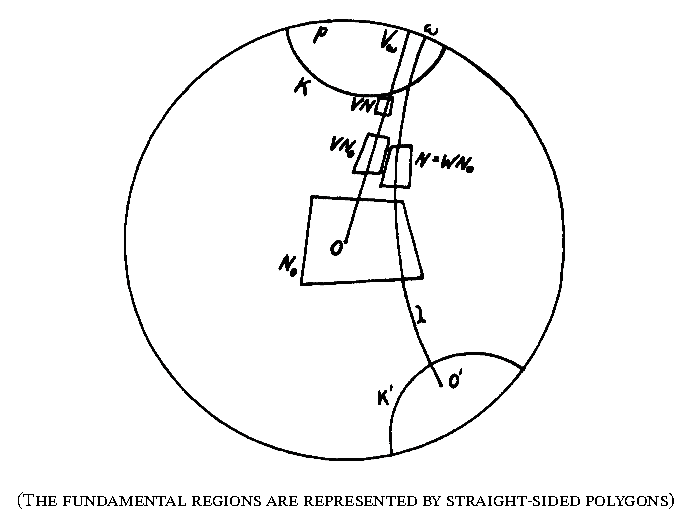
\includegraphics{chap10-vend-scan-01.eps}
\end{figure}

We may also assume that $K$ is small enough to exclude both $N_{0}$ and $N$. Then in particular $O^{\prime}=V^{-1}(O)$ is inside $K^{\prime}$, and so we can draw an $H$-line $\lambda$ from $O^{\prime}$ cutting first $N_{0}$, then $N$. Let $\omega$ be the endpoint of $\lambda$ lying outside $K^{\prime}$. We see that $V\lambda$ is a diameter, and it passes through $0,\,VN_{0},\,VN= VWN_{0}$, and $V\omega$ in that order. It follows that $V\omega\in(W)$. Now $\omega$ is outside $K^{\prime}$, so $V\omega$ is inside $K$. We conclude that every neighborhood of $p$ meets $(W)$, and this is the assertion of the lemma.

\begin{corollary*}
For each $W\in\Gamma$ there is a finite set of polygons
\begin{equation}
\label{ch10:eqn6} V_{1}^{\prime}WN_{0},\qquad V^{\prime}_{2}WN_{0},\,\cdots,\qquad V_{s}^{\prime}WN_{0},
\end{equation}
such that any angle formed of $H$-lines that contains $N_{0}$ contains at least one pair of polygons $V_{i}^{\prime}N_{0},\,V_{i}^{\prime}WN_{0},\,i=1,\ldots,s$, as well as a radius cutting this pair.
\end{corollary*}

The proof is left as an exercise.


\subsection{}\label{ch10:sec3G}
By the \emph{central angle} of a fundamental polygon $N$ we mean the measure of the smallest central angle of $\mathscr{Q}$ that contains $N$---also, the angle itself. In particular the central angle of $N_{0}$ is $2\pi$.

\begin{lemma*}
Let $\delta\geqq 0$ and suppose $N_{1}=V_{1}N_{0}$ and $N_{2}=V_{2}N_{0}$ are two fundamental polygons whose $H$-distance apart is not more than $\delta$. If $\varphi_{i}$ is the central angle of $N_{i}(i=1,2)$, then
\begin{equation*}
0<M\leqq\frac{\varphi_{1}}{\varphi_{2}}\leqq M^{\prime},
\end{equation*}
where $M,\,M^{\prime}$ depend only on $\delta$ and $\Gamma$.
\end{lemma*}

It is obviously sufficient to prove only the lower bound. In the course of the proof we shall have to estimate the euclidean radius $\rho^{\prime}$ of the circle $V(C)$, where $V\in\Gamma, C$ is a circle of radius $\rho$ lying in $\mathscr{U}$, and $V(C)$ lies inside the circle $|z| =r<1$. Let $V=(a\,\overline{c}\,|\,c\,\overline{a})$, let $\alpha$ be the center of $C$, and let $\zeta$ be a point on $C$. We have
\begin{equation*}
2\rho^{\prime}\geqq|V\zeta-V\alpha|=\frac{|\zeta-\alpha|}{|c^{2}(\alpha+\overline{a}/c)(\zeta+\overline{a}/c)|}\geqq\frac{\rho}{|c^{2}|(1+a_{1})^{2}},
\end{equation*}
where
\begin{equation*}
a_{1}=\sup\{|\overline{a}/c|,\quad V\in\Gamma\}
\end{equation*}
is finite and depends only on $\Gamma$ (cf. \eqref{ch10:eqn5}). Reversing the roles of $C$ and $V(C)$ and remembering that $V^{-1}=(\overline{a}, -\overline{c}\,|-c,\, a)$, we get
\begin{equation*}
\frac{1}{a_{2}|c|^{2}}\leqq\frac{\rho^{\prime}}{\rho}\leqq a_{3}|c|^{2},\qquad a_{2}=a_{2}(\Gamma),\qquad a_{3}=a_3(\Gamma).
\end{equation*}
There are only finitely many $V$ that map $C$ inside the circle $|z|=r$; hence $|c|$ is bounded above by a positive constant depending only on $r$. It follows that
\begin{equation}\label{ch10:eqn7}
0<b_{1}<\frac{\rho^{\prime}}{\rho}<b_{2},
\end{equation}
where $b_{1},\,b_{2}$ depend only on $\Gamma$ and $r$. This is the required estimate.

We now return to the polygons $N_{1}$ and $N_{2}$, but consider instead $V_{1}^{-1}N_{1}=N_{0}$ and $V_{1}^{-1}N_{2}=V^{-1}_{1}V_2 N_{0}$. The new polygons are still at an $H$-distance $\leqq\delta$. If $k,\, K\subset\mathscr{U}$ are disks contained in and containing $N_0$, respectively, then both of the circles
\begin{equation*}\tag{$^{\ast}$}
 k,\qquad V^{-1}_{1}V_{2}(K)
\end{equation*}
lie inside the circle $|z|=r$, where $r$ depends only on $\Gamma$ and $\delta$ (and the choice of $K)$. There are only finitely many images of $K$ in this circle, hence the radius of $V_{1}^{-1}V_{2}(K)$ is bounded above and below by positive constants. Now apply the estimate just derived to each of the circles
\begin{equation*}\tag{$\dagger$}
V_{1}(k),\qquad V_{2}(K),
\end{equation*}
which are obtained from the corresponding circles of $(^{\ast})$ by application of $V_{1}$. Denoting the euclidean radii of $(\dagger)$ by $r_{1},\,R_{2}$, and of $(^{\ast})$ by $r_{1}^{\prime},\, R_{2}^{\prime}$, respectively, we find easily
\begin{equation*}
0<b_{3}<\frac{r_{1}}{R_{2}}=\frac{r_{1}}{r_{1}^{\prime}}\frac{r_{1}^{\prime}}{R_{2}^{\prime}}\frac{R_{2}^{\prime}}{R_{2}}<b_{4},
\end{equation*}
where $b_3,\,b_{4}$ are functions of $\Gamma$ and $\delta$ only.

Since $V_{1}(k)$ lies within $N_{1}$, we obviously have $\varphi_1>2r_{1}$. Likewise $\varphi_{2} <bR_{2}$ with $b$ an absolute constant, for clearly $\varphi_{2}/R_{2}\rightarrow 2$ as the polygon $N_{2}$ approaches $\mathscr{Q}$. The two inequalities yield
\begin{equation*}
\frac{\varphi_{1}}{\varphi_{2}}>\frac{2r_{1}}{bR_{2}}>M
\end{equation*}
with $M=M(\Gamma, \delta)$.\:\:\:q.e.d.


\subsection{}\label{ch10:sec3H}
Finally, we prove Theorem~\ref{ch10:sec3B}.

\begin{lemma*}
An arbitrary central angle $\varphi$ contains in its interior a polygon $N_{1}$ whose central angle $\varphi_{1}$ satisfies $\varphi_{1}>b\varphi$, where $b$ is a positive constant depending only on the group $\Gamma$.
\end{lemma*}

Let $\lambda$ be the bisector of $\varphi$. Let $N_{1}$ be the first polygon cutting $\lambda$ that lies entirely within $\varphi$, and let $N_{2}$ be the polygon immediately preceding $N_{1}$ along $\lambda$. Denoting the central angle of $N_i$ by $\varphi_{i}$ we see that $2\varphi_{2}>\varphi$, otherwise $N_{2}$ would lie within $\varphi$. By Lemma~\ref{ch10:sec3G} we have $\varphi_{1}/\varphi_{2}>M$ and so $\varphi_{1}>(M/2)\varphi$. But $M$ depends only on $\delta$ and $\Gamma$, and $\delta =0$ in this case.\:\:\:q.e.d.

Let $\sigma$ be an arbitrary arc of $\mathscr{Q}$ subtending a central angle $\varphi$, and let $N_{1}$ with central angle $\varphi_{1}$ be the polygon of the above lemma. Then
\begin{equation*}\tag{$^{\ast}$}
\varphi_{1}>b\varphi,\qquad b=b(\Gamma).
\end{equation*}
Apply the transformation $V_{1}^{-1}$, where $V_{1}N_{0}=N_{1};\varphi_{1}$ goes into a curvilinear angle $\varphi_{1}^{\prime}$ that contains $N_{0}$ but whose sides pass through vertices of $N_{0}$. The vertex of $\varphi_{1}^{\prime}$ is $O^{\prime}=V_{1}^{-1}(O)$.

Fix an element $W \in\Gamma$. Because of Corollary~\ref{ch10:sec3F} we can assert that $\varphi^{\prime}_{1}$ contains a pair of polygons $V_{i}^{\prime}N_{0},\,V_{i}^{\prime}W N_{0}$ and a radius $O\omega=\mu^{\prime}$ cutting this pair. Through $O^{\prime}$ draw an $H$-line $\lambda^{\prime}$ lying in $\varphi_{1}^{\prime}$ and cutting $V_{i}^{\prime}WN_{0}$; necessarily $\lambda^{\prime}$ cuts $N_{0}$. Apply $V_{1};\ V_{1}\mu^{\prime}=\mu$ is an $H$-line cutting $N_{1},\,V_{i}N_{0},\,V_{i}WN_{0}$, with $V_{i}=V_{1}V_{i}^{\prime}$. Likewise $V_{1}\lambda^{\prime}=\lambda$ is a radius cutting $N_{0},\, N_{1},V_{i}WN_{0}$. Cf. Figures~\ref{ch10:fig1} and~\ref{ch10:fig2}.

Consider the lines $\lambda$ and $\mu$: both lines cut $N_{1}$ and $V_{i}WN_{0}$. Let $D$ be a subregion of $\mathscr{U}$ containing these polygons. Since the $H$-diameter of all fundamental polygons is the same, say $\delta_{0}$, it follows that the $H$-distance between the segments of $\lambda$ and $\mu$ lying in $D$ is less\footnote{The $H$-distance between a point on one line and the foot of its perpendicular dropped on the other line varies monotonely as we approach $\mathscr{Q}$.} than $\delta_{0}$. Therefore there must be a polygon $V_{k} N_{0}$ cut by $\lambda$ and lying between $N_{1}$ and $V_{i} WN_{0}$ whose distance from $V_{i}N_{0}$ is less than $\delta_{0}$, for $\mu$ outs $V_{i}N_{0}$. (Figure~\ref{ch10:fig2}.) Let $V_{k}^{-1}V_{i}=S$. Then the $H$-distance from $SN_{0}$ to $N_{0}$ is less than $\delta_{0}$ and so $S\in\sum$.

\begin{figure}[!h]
\includegraphics{chap10-vend-scan-02.eps}
\caption{}\label{ch10:fig1}
\end{figure}

We now have that $\lambda$ cuts the polygons $V_{k}N_{0},\,V_{k}SWN_{0}$. It follows that the endpoint of $\lambda$ belongs to $[W]$. By rereading the argument one can see that each radius $\lambda$ cutting $V_{i}WN_{0}$ has this property. That is, the arc $\sigma_{i}$ of $\mathscr{Q}$ subtended by the central angle $\varphi_{i}$ of $V_{i}WN_{0}$ consists entirely of points belonging to $[W]$.

The $H$-distance between $N_{1}$ and $V_{i}WN_{0}$ is equal to the $H$-distance between $N_{0}$ and $V_{1}^{-1}V_{i}WN_{0}=V^{\prime}_{i} WN_{0}$, and so is not more than the maximum distance $\delta_{1}=\delta_{1}(W)$ from $N_{0}$ to the polygons of the set \eqref{ch10:eqn6}. Hence by Lemma~\ref{ch10:sec3G} we get
\begin{equation*}
\varphi_{i}/\varphi_{1}\geqq M,\qquad M=M(\delta_{1}).
\end{equation*}
With $(^{\ast})$ this gives
\begin{equation*}
\varphi_{i}\geqq M^{\prime}\varphi,\qquad M^{\prime}=M^{\prime}(\Gamma).
\end{equation*}
Since $|\sigma_i|=\varphi_{i},\,|\sigma|=\varphi$, we see that Theorem~\ref{ch10:sec3B} is proved.


\subsection{}\label{ch10:sec3I}
Myrberg\index{Myrberg} has also proved the following theorem. If $\Gamma$ \emph{has a fundamental region with a finite number of vertices all lying on} $\mathscr{Q}$, \emph{then} $\mathbf{I}$ \emph{is uncountable}. For the proof we refer the reader to the original paper: [\citeauthor{Myrberg0000}~\ref{Myrberg2}, pp. 408--9]. The result is doubtless true in the general case. It shows, in particular, that there are points on $\mathscr{Q}$, other than parabolic vertices, which are intransitive.

\begin{figure}[!h]
\includegraphics{chap10-vend-scan-03.eps}
\caption{}\label{ch10:fig2}
\end{figure}


\section{The Automorphic Function near the Boundary}\index{automorphic function!near boundary}\label{ch10:sec4}
\subsection{}\label{ch10:sec4A}
Let $f(z)$ be a nonconstant function automorphic on $\Gamma$. We suppose $\Gamma$ is defined on $\mathscr{U}$. Let $\alpha$ be a transitive point\index{transitive point} of $\Gamma$ and $L$ an $H$-ray through $\alpha$. The images of the points on $L$ under $\Gamma$ lie everywhere dense in $\mathscr{U}$. Therefore the values of $f(z)$ for $z$ on $L$ are everywhere dense in the totality of values assumed by $f(z)$ for $z\in \mathscr{U}$. Since a nonconstant automorphic function assumes each complex number at least once (\ref{ch05:chap05}. Th. \ref{ch05:sec4H}), we have:

\begin{theorem*}
If $\alpha$ is a transitive point of $\Gamma$ and $L$ is an $H$-ray through $\alpha$, then the set of values assumed by a nonconstant automorphic function $f(z)$ for $z$ on $L$ is everywhere dense in the set of complex numbers.
\end{theorem*}

Thus $f$ does not tend to a limit on radial approach (say) to a transitive point; in fact, $f$ is completely indeterminate in the neighborhood of such a point. What of the intransitive points? At a parabolic vertex we know that an automorphic function tends to a definite value (\ref{ch05:chap05}. Th. \ref{ch05:sec1C}). At a point that is intransitive but not parabolic the behavior of the function is in general unknown, except that the set of its values is not dense in the set of all values assumed by the function. But for special groups we can make a definite statement. In \ref{ch10:sec4B}--\ref{ch10:sec4D} we consider only the modular group.


\subsection{}\label{ch10:sec4B}
\begin{theorem*} A modular function\index{modular function!near boundary}\footnote{A modular function is an automorphic function on the modular group (\ref{ch03:chap03}. \ref{ch03:sec1F}). The modular group\index{Hecke group} is defined on $\mathscr{H}$ rather than $\mathscr{U}$.} fails to approach a limit on vertical approach to a real irrational point. In fact, if $\alpha$ is irrational, if $L$ is the vertical line ending at $\alpha$, and if $f$ is a modular function, then the derived set of $f(L)$ is uncountable.
\end{theorem*}

We shall require a few facts about continued fractions; these may all be found on page 25 of \citeauthor{Koksma0000}~[\ref{Koksma1}]\index{Koksma}. Let
\begin{equation*}
\alpha=[b_{0}, b_{1}, \cdots]
\end{equation*}
be the regular continued fraction expansion of the irrational number $\alpha$, and let $\{p_{n}/q_{n}\}$ be its convergents. Note that $p_{n}$ is prime to $q_{n}$. We consider the sequence
\begin{equation*}
z_{n}(c)=z_{n}=\alpha+iy_{n},\qquad y_{n}=c|\alpha-p_{n}/q_{n}|,\qquad c\,>0.
\end{equation*}
Since $\alpha$ is irrational, we have
\begin{equation*}\tag{$^{\ast}$}
\frac{1}{(q_{n+1}+q_{n}) q_{n}}<\bigg|\alpha-\frac{p_{n}}{q_{n}}\bigg|<\frac{1}{q_{n}q_{n+1}};
\end{equation*}
hence $y_{n}\rightarrow 0,\,y_{n}>0$. Thus $z_{n}\rightarrow\alpha$ vertically. Construct the matrix $V_{n}=(q_{n}^{\prime}, -p_{n}^{\prime}|q_{n}, -p_{n})$ of determinant 1, where for each $n$ the integers $q_{n}^{\prime},\,-p_{n}^{\prime}$ are such that $|{\rm Re}\, V_{n}z|\leqq 1/2$. $V_{n}$ is an element of $\Gamma(1)$, the modular group. Set $V_{n}z_{n}=z_{n}^{\prime}=x_{n}^{\prime}+iy_{n}^{\prime}$.

Now
\begin{align*}
&y_{n}^{\prime}=\frac{y_{n}}{q_{n}^{2}\{(\alpha-p_{n}/q_{n})^{2}+y_{n}^{2}\}}=\frac{1}{q_{n}^{2}|\alpha-p_{n}/q_{n}|}\cdot\frac{1}{c+1/c}|=A_{n}C,\\
&\qquad\qquad\qquad\qquad\qquad\quad C=\frac{1}{c+1/c}\cdot
\end{align*}
According to $(^{\ast})$,
\begin{equation*}
\frac{q_{n+1}}{q_{n}}<A_{n}<1+\frac{q_{n+1}}{q_{n}}.
\end{equation*}
We now divide the discussion into two cases.

I. $b_{n}\leqq M,\,n=1,2,\cdots$.

Then, since $q_{n+1}=b_{n+1}q_{n}+q_{n-1}$, we have
\begin{equation*}
1\leqq b_{n+1}<A_{n}<M+2.
\end{equation*}
Let $A^{\prime}$ be any limit point of $(A_{n})$ and let $A_{p}\rightarrow A^{\prime}$. Then $y_{p}^{\prime}\rightarrow A^{\prime}C$. On a further subsequence $z_{q}^{\prime}(c)\rightarrow w_{c}=x_{c}+iA^{\prime} C$, where $|x_{c}|\leqq 1/2$.

If we restrict $c$ to a range $0<c_{0}\leqq c\leqq c_{1}<\infty$, the numbers $A^{\prime}C$ are bounded above and below by positive constants. Hence the set $S= \{w_{c}|c_{0}\leqq c\leqq c_{1}\}$ lies in a finite number of fundamental regions of the modular group. The subset $S^{\prime}$ consisting of all inequivalent points of $S$ is therefore uncountable. In view of $f(z_{n}(c))=f(z_{n}^{\prime}(c))$, we have that $d(f(L))$, the derived set of $f(L)$, contains $f(S^{\prime})$. But $f$ is of finite valence (\ref{ch05:chap05}. Th. \ref{ch05:sec4H}; proof of \ref{ch05:chap05}. Th. \ref{ch05:sec4C}). Therefore $d(f(L))$ is uncountable.

II. There is a subsequence $b_{n_{i}}\rightarrow\infty$.

In this case $q_{m_{i}}/q_{m_{i}-1}\rightarrow\infty$ so that from $(^{\ast})$, $q_{m_{i}-1}^{2}|\alpha-p_{m_{i}-1}/q_{m_{i}-1}|\rightarrow 0$. Select $y_{i}(c)=1/cq_{m_{i}-1}^{2}, V_{i}=(\cdot\ \cdot |q_{m_{i}-1}, -p_{m_{i}-1})$. Then $y_{i}^{\prime}(c)\rightarrow c$. The proof now goes through as before.\:\:\:q.e.d.

The above proof is due to Epstein and Lehner\index{Epstein-Lehner} [\ref{Epstein1}]; cf. also H. \citeauthor{Cohn0000}~[\ref{Cohn1}]\index{Cohn, H.}. David\index{Rosen, David} \citeauthor{Rosen0000}~[\ref{Rosen1}] has extended the result to the Hecke groups $G(\lambda)$; these are the groups generated by $z^{\prime}=z+\lambda,\, z^{\prime}=-1/z$, where either $\lambda>2$ or $\lambda=2\cos\pi/q,\,q=3,4,5,\cdots$.


\subsection{}\label{ch10:sec4C}
By the same methods results can be obtained for modular forms.\index{modular form!near boundary}

\begin{theorem*}
Let $\alpha$ be irrational, $F(z)$ a form of positive dimension that has a pole at $i\infty$. If the continued fraction expansion for $\alpha$ has unbounded denominators, $F$ does not tend to a limit on vertical approach to $\alpha$. If $\alpha$ has bounded partial denominators and in addition $F$ has no finite poles, then $F(z)\rightarrow 0$ as $z\rightarrow\alpha$ in any Stolz angle \emph{(}i.e., a wedge of angle $<\pi$ with apex at $\alpha)$.
\end{theorem*}

For the proof see [\citeauthor{Rosen0000}~\ref{Rosen1}, pp. 378--379].


\subsection{}\label{ch10:sec4D}
It is easy to extend Theorem~\ref{ch10:sec4B} to subgroups of finite index in the modular group $\Gamma(1)$. Let $H$ be the subgroup. We have seen in the proof of Theorem~\ref{ch10:sec4B} that there exist sequences $z_{q}(c)\rightarrow\alpha$ such that $z_{q}^{\prime}(c)= V_{q}z_{q}(c) \rightarrow w_{c}$, the set $\{w_{c}\}$ being uncountable. Since $H$ is of finite index, infinitely many $V_{q}$ lie in some coset of $\Gamma(1)\backslash H$. That is, there is a sequence $z_{r}(c)={V_{r}}^{-1}z_{r}^{\prime}(c)=T_{r}Az_{q}^{\prime}(c)$ with $Tr \in H, A\in\Gamma(1)$. Hence if $g$ is automorphic on $H$, we have $g(z_r(c))=g(Az_{r}^{\prime}(c))\rightarrow g(Aw_{c})$. Points of $\{Aw_{c}\}$ inequivalent under $\Gamma(1)$ are inequivalent under $H$, and so there are uncountably many. Now $g$ is of finite valence. Hence the distinct values in $\{g(Aw_{c})\}$ are uncountable in number and the conclusion follows.

\begin{theorem*}
Theorem~\emph{\ref{ch10:sec4B}} is valid for functions automorphic on a subgroup of finite index in the modular group.\index{modular function!near boundary}
\end{theorem*}


\subsection{}\label{ch11:sec4E}
We have been considering orthogonal approach to a boundary point. The other extreme is approach along a curve tangent to the principal circle.

~\citeauthor{Hedlund0000}~[\ref{Hedlund1}] has considered in detail the special case of horocycles (euclidean circles tangent internally to $\mathscr{U}$). \emph{If} $C_{q}$ \emph{is a horocycle tangent to} $\mathscr{Q}$
\emph{at} $q$ \emph{and} $\alpha\neq q$ \emph{is any point on} $C_{q}$, \emph{then a nonconstant automorphic function} $f$ \emph{approaches every complex number as} $z\rightarrow q$ \emph{on the arc} $\alpha q$, \emph{provided} $q$ \emph{is not a parabolic vertex of} $\Gamma$. The proof uses geometrical arguments.


\skiptoctrue
\section*{Exercise}

1. An automorphic function\index{Hedlund} does not tend to a limit on any arc of a horocycle tangent to $\mathscr{U}$ at a parabolic vertex.

\section{Diophantine Approximation}\label{ch10:sec5}

In this Section $\Gamma$ may be horocyclic or not: $\infty$ is a parabolic vertex.\index{diophante approximation}

\subsection{}\label{ch10:sec5A}
A classical result in number theory is the following: to each real irrational number $\alpha$ there corresponds a sequence of distinct reduced fractions $p_{n}/q_{n}$ such that
\begin{equation}\label{ch10:eqn8}
\bigg|\alpha-\frac{p_{n}}{q_{n}}\bigg|<\frac{1}{hq_{n}^{2}},\qquad n=1,2,\cdots
\end{equation}
where $h$ is an absolute positive constant. According to results of A. Hurwitz the best possible value for $h$ is $h=\sqrt{}\,5$. Obviously \eqref{ch10:eqn8} has only a finite number of solutions $p/q$ if $\alpha$ is rational.

In 1952 \citeauthor{Lehner0000}~[\ref{Lehner1}]\index{Lehner} proposed the following generalization:

\begin{theorem*}
Let $\Gamma$ be defined on the upper half-plane $\mathscr{H}$. As usual we denote the set of limit points and the set of parabolic vertices of $\Gamma$ by $\mathscr{L}$ and $\mathscr{P}$, respectively. To each number $\alpha\in \mathscr{L}-\mathscr{P}$ there corresponds a sequence of distinct parabolic vertices $-d_{n}/c_{n}\in \mathscr{P}$ such that
\begin{equation}
\label{ch10:eqn9} \bigg|\alpha+\frac{d_{n}}{c_{n}}\bigg|<\frac{1}{hc_{n}^{2}},
\end{equation}
where $h$ is a positive constant depending only on $\Gamma$.
\end{theorem*}

\noindent It is seen that \eqref{ch10:eqn9} reduces to \eqref{ch10:eqn8} when $\Gamma$ is the modular group, in which case $\mathscr{P}$ is the set of rationals and $\mathscr{L}$ the set of reals.

Lehner's proof of the theorem contains a gap (namely, in the proof of Lemma~\ref{ch10:sec5B} below). However, the theorem is true, as we shall now show. Meanwhile \citeauthor{Rankin0000}~[\ref{Rankin1}]\index{Rankin} published a proof in 1957 for horocyclic $\Gamma$.


\subsection{}\label{ch10:sec5B}
\begin{lemma*}
Let $U^{\lambda}=(1\ \lambda\,|\,0\ 1)$ generate $\Gamma_{\infty}$, the subgroup of $\Gamma$ that fixes $\infty$. Let $\alpha$ be real, $\alpha\not\in \mathscr{P}$. There is a sequence $z_{n}=\alpha+iy_{n}\ (y_{n}>0)$ and corresponding $V_{n}\in\Gamma$, belonging to infinitely many different cosets of $\Gamma_{\infty}\backslash \Gamma$, such that $z_{n}\rightarrow\alpha$ and
\begin{equation*}
y_{n}^{\prime}={\rm Im}\ V_{n}z_{n}>h/2,
\end{equation*}
where $h$ depends only on $\Gamma$.
\end{lemma*}

We recognize this result as the upper half-plane version of \ref{ch05:chap05}. Th. \ref{ch05:sec5G}. We have only to prove that if $V_{n}=(a_{n}\,b_{n}|c_{n}\,d_{n})$ we have $(c_{n+p}, d_{n+p})\neq(c_{n}, d_{n})$ for $p$ large enough. Indeed, $V_{n}$ maps the segment $\alpha+iy,\, 0\leqq y\leqq\varepsilon$, on an arc ending at a real finite point. Since $y_{n}\rightarrow 0$ we can find $y_{n+p}$ so small that ${\rm Im}\ V_{n}z_{n+p}\leqq h/2$. Hence
\begin{equation*}\tag{$^{\ast}$}
{\rm Im}\ V_{n+p}z_{n+p}\neq{\rm Im}\ V_{n}z_{n+p}.
\end{equation*}
Now ($c_{n+p},\,d_{n+p})=(c_{n}, d_{n})$ would imply $V_{n+p}=U^{m\lambda}V_{n}$ for an integer $m$ and this contradicts $(^{\ast})$.

We can therefore select an infinite subsequence $(V_{m})$ consisting entirely of elements with different second row. Theorem~\ref{ch10:sec5A} is now an easy consequence. For the arithmetic mean is not less than the geometric mean; thus
\begin{equation}
\label{ch10:eqn10} 2|c_{m}\alpha+d_{m}|\ |c_{m}y_{m}|\leqq(c_{m}\alpha+d_{m})^{2}+c_{m}^{2}y_{m}^{2}=y_{m}/y_{m}^{\prime}<2y_{m}/h,
\end{equation}
from which \eqref{ch10:eqn9} follows immediately.

\emph{Remark}. The numbers $-d_{m}/c_{m}$ are images of $\infty$. In Theorem~\ref{ch10:sec5A}  we claimed only that they were parabolic vertices. Our result is actually a little stronger than what is asserted in the theorem.


\subsection{}\label{ch10:sec5C}
From Theorem~\ref{ch10:sec3A} we shall now deduce a result which is stronger than Theorem~\ref{ch10:sec5A} in one respect, weaker in another. Let $\Gamma$ be \emph{horocyclic}.

We can define transitive and intransitive points\index{transitive point} on $\mathscr{E}$ (the real axis) exactly as we did on $\mathscr{Q}$---cf. \ref{ch10:sec1B}. Theorem~\ref{ch10:sec3A}, when stated for groups on $\mathscr{H}$, takes the form: \emph{almost all real numbers are transitive}.

\begin{theorem*}
$\Gamma$ is horocyclic. Let $\alpha$ be a transitive point and let $(\varepsilon_{n})$ be a sequence of positive numbers $\rightarrow 0$. There exists a sequence of different $-d_{n}/c_{n}\in \mathscr{P}$ such that
\begin{equation}
\label{ch10:eqn11} \bigg|\alpha+\frac{d_{n}}{c_{n}}\bigg|<\frac{\varepsilon_{n}}{c_{n}^{2}},\,\qquad
n=1,2,\cdots
\end{equation}
In particular, the result holds for almost all $\alpha$.
\end{theorem*}

Let $H_{n}$ be a circle orthogonal to $\mathscr{E}$ of radius $1/\varepsilon_{n}$, and let $L_{\alpha}$ be the vertical line $\{x=\alpha, y>0\}$. For almost all $\alpha$ there are images $V_{n}(L_{\alpha})$ which approximate $H_{n}$. Since the $H_{n}$ have different radii we can select the $V_{n}$ so that they have different second row. There is a point $z_{n}=\alpha+iy_{n}$ on $L_{\alpha}$ such that $z_{n}^{\prime}=V_{n}(z_{n})$ has imaginary part greater than $1/2\varepsilon_{n}$. Then, with $V_{n}=(\cdot\ \cdot\, |\,c_{n}\ d_{n})$, the inequality \eqref{ch10:eqn10} gives
\begin{equation*}
2|c_{n}\alpha+d_{n}|\,|c_{n}y_{n}|\leqq y_{n}/{\rm Im}\, z_{n}^{\prime}<2\varepsilon_{n}y_{n},
\end{equation*}
which is the desired result.

The inequality \eqref{ch10:eqn11} is much stronger than \eqref{ch10:eqn9}; indeed, it is equivalent to \eqref{ch10:eqn9} with arbitrarily large $h$. However, the exceptional set of $\alpha$ is only known to be of measure $0$; it may contain, besides $\mathscr{P}$, an uncountable set (cf. \ref{ch10:sec3I}). Furthermore, the theorem has been proved only for horocyclic groups. Note that the full strength of Theorem~\ref{ch10:sec3A} was not used in the proof. All that we needed was a sequence $z_{n}\rightarrow\alpha$ such that ${\rm Im}\, z_{n}^{\prime}\rightarrow+\infty$.

If $\Gamma$ is the modular group, inequalities similar to \eqref{ch10:eqn11} are available from number theory. For example, Khintchine's\index{Khintchine} theorem tells us that almost all real $\alpha$ admit the approximation
\begin{equation}\label{ch10:eqn12}
 \bigg|\alpha+\frac{d_{n}}{c_{n}}\bigg|<\frac{1}{c_{n}^{2}\log c_{n}},\, \qquad n=1,2,\cdots
\end{equation}
$d_{n}/c_{n}$ being reduced fractions (cf. \citeauthor{Koksma0000}~[\ref{Koksma1}\index{Koksma}, p. 47]). Since it does not seem possible to express $\varepsilon_{n}$ as a function of $c_{n}$, a direct comparison of \eqref{ch10:eqn11} and \eqref{ch10:eqn12} is ruled out.

Returning to Theorem~\ref{ch10:sec5A}, we see that if \eqref{ch10:eqn9} holds for a certain $h$, it holds for all smaller $h$. We are therefore interested in the supremum of $h$. This has been investigated by \citeauthor{Rankin0000}~[\ref{Rankin1}]\index{Rankin} who found that
\begin{equation*}
h_{\Gamma}\leqq\sup h\leqq h_{\Gamma}^{\prime}.
\end{equation*}
To define these constants, let $R_0$ be a fundamental region of $\Gamma$ with cusp at $i\infty$. $R_{0}$ may contain certain elliptic vertices lying in $\mathscr{H}$. It may also happen that some sides of $R_{0}$ are complete semicircles; in this case, we also call the highest point of the semicircle a vertex. Then $h_{\Gamma}$ is defined to be twice the minimum distance from $\mathscr{E}$ of the vertices of $R_{0}$ in $\mathscr{H}$. Now let $H=(a\ b\, |\,c\ d)$ run over the hyperbolic elements of $\Gamma$ and define
\begin{equation*}
\rho_{H}=\frac{[(a+d)^{2}-4]^{1/2}}{|c|}\cdot\max\bigg\{1,\frac{c^{2}}{\tilde{c}^{2}(|a+d|-2)}\bigg\},
\end{equation*}
where $\tilde{c}$ is the minimum value of $|c|\neq 0$ for all transformations of $\Gamma$. Then
\begin{equation*}
h_{\Gamma}^{\prime}=\inf\rho_{H}.
\end{equation*}

For the modular group, these constants work out to be
\begin{equation*}
h_{\Gamma}=\sqrt{}\,3,\qquad h_{\Gamma}^{\prime}=\sqrt{ }\,5.
\end{equation*}
Actually $\sup h=\sqrt{}\,5$.


%%%%%%%%%%chapter11

\chapter{The Modular Group and Modular Functions}\label{ch11:chap11}\index{modular group}\index{modular function}

The modular group was the first discontinuous group (except for the simply and doubly periodic groups) to be subjected to intensive scrutiny. It is still almost the only group we know very much about. In this chapter we shall include mostly investigations of the modular group and its analytical invariants that take advantage of its arithmetical characterization. Generally speaking, these have not yet been extended to arbitrary $H$-groups.

We use the term ``modular group'' loosely to include both the full group $\Gamma(1)$ and its subgroups. \emph{Throughout this chapter we shall denote the full modular group by} $\Gamma$. The reader may refresh his memory by consulting \ref{ch03:chap03}. \ref{ch03:sec1F} for the definition and \ref{ch04:chap04}. \ref{ch04:sec5H} for the form of the fundamental region $R_{0}$. The modular group may be presented as
\begin{equation*}
\Gamma=\{-I,\, U,\, T;\quad (-I)^{2}=I,\quad T^{2}=(TU)^{3}=-I\},
\end{equation*}
where
\begin{equation*}
U=\left(\begin{matrix}
1 & 1\\
0 & 1
\end{matrix}\right),\qquad T=\left(\begin{matrix}
0 & -1\\
1 & \ \ 0
\end{matrix}\right).
\end{equation*}

\section{Modular Forms}\index{modular form}\label{ch11:sec1}

\subsection{}\label{ch11:sec1A}
A convenient approach to the theory of modular forms is through the Eisenstein-Weierstrass\index{Eisenstein series} invariants (\ref{ch08:chap08}. \ref{ch08:sec3L}) which, however, we now normalize slightly differently:
\begin{equation*}
g_{k}(\tau)=A\,{_{k}\tilde{g}}_{k}(\tau),
\end{equation*}
where the $A_{k}$ are certain numerical factors occurring in the Taylor series for the Weierstrass function $\wp$ (cf. [\citeauthor{Fricke0000}~\ref{Fricke2},\index{Fricke} p. 262]). In particular $A_{2}=60,\ A_{3}=140$, so that
\begin{equation}\label{ch11:eqn1}
g_{2}(\tau)=60\sideset{}{^{\prime}}\sum\limits_{c,d}\,(c\tau +d)^{-4},\qquad g_{3}
(\tau)=140\sideset{}{^{\prime}}\sum\limits_{c,d}(c\tau+d)^{-6},
\end{equation}\index{$g_{2}(\tau),g_{3}(\tau)$}
where $\sum^{\prime}$ indicates a sum over all integer pairs ($c,\, d)$ except
(0,0). The functions $g_{k}$ belong to $\{\Gamma, -2k, 1\}$; they are regular in\footnote{$\mathscr{H}^{+}=\mathscr{H}\cup\mathscr{P};\mathscr{H}$ is the upper half-plane and $\mathscr{P}$ the set of parabolic vertices. In the case of the modular group, $\mathscr{P}$ \emph{is} the set of rational numbers and $\infty$.} $\mathscr{H}^{+}$.

We wish to produce a cusp form\footnote{A form that vanishes on $\mathscr{P}$. The vector space of cusp forms is denoted by $\mathbb{C}^{0}(\Gamma,\, -r,\, v)$.} of lowest possible dimension with multipliers identically 1. There are no cusp forms of dimension greater than $-12$, but there is one of this dimension (\ref{ch08:chap08}. \ref{ch08:sec6A}. $(^{\ast\ast}))$. It is\footnote{Cf. footnote to formula \eqref{ch11:eqn13}, \ref{ch11:sec1E}.}
\begin{equation}
\label{ch11:eqn2} \Delta(\tau)=(2\pi)^{-12}\{g_{2}^{3}(\tau)-27g_{3}^{2}(\tau)\}=t +\cdots,\quad t=e(\tau).
\end{equation}\index{$\Delta(\tau)$}
We have used in this calculation the Fourier expansions of $g_{2}$ and $g_{3}$ (\ref{ch08:chap08}. \ref{ch08:sec3L}).

The function $\Delta$ occurs in the Weierstrassian theory of elliptic functions as the discriminant of a polynomial known to have distinct zeros. Hence $\Delta$ is never $0$. Thus we are not surprised to learn that $\Delta$ can be expressed as an infinite product:
\begin{equation}\label{ch11:eqn3}
\Delta(\tau)=e(\tau)\prod_{m=1}^{\infty}(1-e(m\tau))^{24},\qquad\ {\rm Im}\ \tau>0.
\end{equation}

In our development, however, we shall not take this route. Instead we shall \emph{define} $\Delta$ by equation \eqref{ch11:eqn3} and prove directly that $\Delta\in \mathbb{C}^{0}(\Gamma,\, -12,\,1)$. Then \eqref{ch11:eqn2} will follow. For there is only one linearly independent cusp form in $\{\Gamma,\, -12,\,1\}$ that is regular in $\mathscr{H}$. Thus the $\Delta$ defined by \eqref{ch11:eqn2} is a constant multiple of the $\Delta$ defined by \eqref{ch11:eqn3} and a numerical control of the coefficients shows them to be equal.


\subsection{}\label{ch11:sec1B}
The function $\Delta$ was first studied extensively by \citeauthor{Dedekind0000}~[\ref{Dedekind1}] and \citeauthor{Hermite0000}~[\ref{Hermite2}]\index{Hermite}. They took the 24th root, defining a function
\begin{equation}\label{ch11:eqn4}
\eta(\tau)=e(\tau/24)\prod_{m=1}^{\infty}(1-e(m\tau)),\qquad {\rm Im}\ \tau >0.
\end{equation}\index{modular form!$\eta(\tau)$}
We wish to prove that $\eta \in\{\Gamma,\ -1/2,\ v_{0}\}$, where $v_{0}$ is a certain multiplier system, and to determine the explicit dependence of $v_{0}(M)$ on the coefficients of the modular substitution $M$.

Dedekind\index{Dedekind} went even further and studied $\log \eta(\tau)$. Since $\eta$ never vanishes in $\mathscr{H},\, \log\eta$ is a uniform function. Dedekind determined completely the behavior of $\log\eta$ under modular transformations. This is more difficult than the equivalent problem for $\eta$, since certain additive multiples of $2\pi i$ in the transformation equation for $\log\eta$ are absorbed on exponentiation and do not appear in the equation for $\eta$.

Many proofs of the transformation formula for $\log\eta$ have appeared since the classical investigations of Dedekind and Hermite. We shall present a recent one by \citeauthor{Rademacher0000}~[\ref{Rademacher8}],\index{Rademacher} which extends to all modular substitutions an argument given by \citeauthor{Siegel0000}~[\ref{Siegel3}]\index{Siegel} for the transformation $\tau \rightarrow-1/\tau$.


\subsection{}\label{ch11:sec1C}
We write the general modular substitution in the form
\begin{equation*}
\tau^{\prime}=M\,\tau,\qquad M=\left(\begin{matrix}
h^{\prime} & -(hh^{\prime}+1)/k\\
k & -h
\end{matrix}\right)
\end{equation*}
with $h,\,h^{\prime},\,k$ integers, $k>0,\,h$ prime to $k$, and $h^{\prime}$ a fixed solution of the congruence
\begin{equation*}
hh^{\prime}\equiv-1\quad (\mathrm{mod}\ k).
\end{equation*}
The case $k=0$, i.e., $M_{\tau}=\tau +m$, is trivial: $v_{0}(M)=e(m/24)$.

Set
\begin{equation*}
\tau=(h+iz)/k.
\end{equation*}
Then ${\rm Im}\ {\tau} >0$ is equivalent to
\begin{equation*}
\mathrm{Re}\ z>0,
\end{equation*}
which we assume from now on. Hence
\begin{equation*}
\tau^{\prime}=(h^{\prime}+iz^{-1})/k.
\end{equation*}
In terms of this\index{multiplier system!on modular group} notation the transformation equation we want to prove takes the form
\begin{equation}
\begin{split}
\log\eta((h^{\prime}+iz^{-1})/k)=&\log\eta((h+iz)/k)+\frac{1}{2}\log z\\
&+\pi i(h^{\prime}-h)/12k +\pi is(h, k),\label{ch11:eqn5}
\end{split}
\end{equation}\index{modular form!$\eta(\tau)$}
where $s(h, 1)=0$, and for $k>1,\ s(h,k)$ is the ``Dedekind sum''\index{Dedekind sum}
\begin{equation}\label{ch11:eqn6}
s(h, k)=\sum\limits_{\mu=1}^{k-1}\left(\frac{\mu}{k}-\frac{1}{2}\right)\left(\frac{\mu
h}{k}-\left[\frac{\mu h}{k}\right]-\frac{1}{2}\right).
\end{equation}
As usual the branch\index{modular group!multiplier system on} of the logarithm is fixed by our convention: $-\pi\leqq \arg z<\pi;[x]$ is the greatest integer $\leqq x$.

For purposes of abbreviation we shall use both
\begin{equation*}
\varepsilon(u)=e^{-2\pi u},\qquad e(u)=e^{2\pi iu}.
\end{equation*}
From the definition \eqref{ch11:eqn4} we get, on setting $m=qk+\mu,\ q=0,\,1,\cdots,\mu =1,2,\cdots,\,k$,
\begin{equation*}
\log\,\eta\bigg(\frac{h+iz}{k}\bigg)-\frac{\pi i(h+iz)}{12k}=\sum\limits_{\mu=1}^{k}
\sum\limits_{q=0}^{\infty}\,\log\left\{1-e\left(\frac{h\mu}{k}\right)\varepsilon\left(\frac{z(qk+\mu)}{k}\right)\right\}.
\end{equation*}
Replace the logarithm by its power series and obtain for the right member,
\begin{align*}
-\sum\limits_{\mu}\sum\limits_{q}\sum\limits_{l=1}^{\infty}\frac{1}{l}e\left(\frac{h\mu l}{k}\right)\varepsilon & \left(\frac{z(qk+\mu)l}{k}\right)\\
&\quad =-\sum\limits_{\mu}\sum\limits_{l}\sum\limits_{q=0}^{\infty}=-\sum\limits_{u= 1}^{k}\sum\limits_{l=1}^{\infty}\frac{1}{l}e\left(\frac{h\mu l}{k}\right)\frac{\varepsilon(z\mu l/k)}{1-\varepsilon(zl)}.
\end{align*}
Thus equation \eqref{ch11:eqn5} is equivalent to
\begin{align}
&\sum\limits_{\nu=1}^{k}\sum\limits_{l=1}^{\infty}\frac{1}{l}e(h^{\prime}\nu
l/k)\frac{\varepsilon(\nu l/kz)}{1-\varepsilon(l/z)}\nonumber\\
&-\sum\limits_{\mu=1}^{k}\sum\limits_{l=1}^{\infty}\frac{1}{l}e(h\mu l/k)\frac{\varepsilon(\mu zl/k)}{1-\varepsilon(lz)}\label{ch11:eqn7}\\
&+\pi(z^{-1}-z)/12k+\pi i\,s(h, k)=-\frac{1}{2}\log z\nonumber.
\end{align}\index{$\nu_{0}$}
This is the equation we shall prove.

Let $C$ be the parallelogram with vertices $z,\,i,\,-z,\,-i$. We introduce the function
\begin{equation}\label{ch11:eqn8}
F_{n}(x)=-\frac{1}{4ix}\coth\,\pi Nx\cot\frac{\pi Nx}{z}+\sum\limits_{\mu=1}^{k-1}\frac{1}{x}
\frac{\varepsilon(-\mu Nx/k)}{1-\varepsilon(-Nx)}\frac{e(-\mu^{\ast}Nx/kz)}{1-e(-Nx/z)},
\end{equation}
where $N=n+1/2$. For $k=1$ the sum is empty. For $k>1,\,\mu^{\ast}$ is defined uniquely by
\begin{equation*}
\tag{$^{\ast}$} \mu^{\ast}\equiv h\mu\ (\mathrm{mod}\ k),\qquad 1\leqq\mu^{\ast}<k.
\end{equation*}
When $n \rightarrow\infty$, the sum of the residues of $F_{n}(x)$ in $C$ tends to $1/\pi i$ times the left member of \eqref{ch11:eqn7}, as we now demonstrate.

The function $F_{n}(x)$ has a pole of third order at $x=0$. A somewhat lengthy calculation yields for the residue,
\begin{align*}
\mathrm{Res}\ F_{n}(0)=- \frac{1}{12i}&\left(z-\frac{1}{z}\right)+zi\sum\limits_{\mu=1}^{k-1}
\left(\frac{1}{12}-\frac{\mu}{2k}+\frac{\mu^{2}}{2k^{2}}\right)\\
\tag{$^{\ast\ast}$}&\quad+\frac{1}{zi}\sum\limits_{\mu=1}^{k-1}\left(\frac{1}{12}-\frac{\mu^{\ast}}{2k}+\frac{\mu^{\ast
2}}{2k^{2}}\right)+\sum\limits_{\mu=1}^{k-1}\left(\frac{\mu}{k}-\frac{1}{2}\right)\left(\frac{\mu^{\ast}}{k}-\frac{1}{2}\right).
\end{align*}
We observe at this point that $\mu^{\ast}$ runs from 1 to $k-1$ when $\mu$ runs over the same range. Furthermore we clearly have
\begin{equation*}
\frac{h\mu}{k}-1<\frac{h\mu}{k}-\frac{\mu^{\ast}}{k}<\frac{h\mu}{k}
\end{equation*}
and, since $(h\mu-\mu^{\ast})/k$ is an integer, this gives
\begin{equation*}
\frac{\mu^{\ast}}{k}=\frac{h\mu}{k}-\left[\frac{h\mu}{k}\right].
\end{equation*}
Hence the last sum in the right member of $(^{\ast\ast})$ is just $s(h, k)$. The first two sums are elementary and we get finally
\begin{equation}\label{ch11:eqn9}
\mathrm{Res}\ F_{n}(0)=\frac{1}{12k}\left(zi+\frac{1}{zi}\right)+s(h,\, k).
\end{equation}
The remaining poles of $F_{n}(x)$ in $C$ are located at
\begin{equation*}
x=il/N,\qquad x=-zl/N,\qquad l=\pm\, 1,\,\pm\, 2,\cdots, \pm\,n.
\end{equation*}
These are simple poles, and we have
\begin{equation*}
\mathrm{Res}\ F_{n}\left(\frac{il}{N}\right)=\frac{1}{4\pi l}\cot\frac{\pi il}{z}-\frac{1}{2\pi i}\sum\limits_{\mu=1}^{k-1}\frac{1}{l}e\left(\frac{\mu l}{k}\right)\frac{\varepsilon(-\mu^{\ast}l/kz)}{1-\varepsilon(-l/z)}.
\end{equation*}
In view of $(^{\ast})$ we have $h^{\prime}\mu^{\ast}\equiv hh^{\prime}\mu\equiv-\mu\,(\mathrm{mod}\ k)$. Hence
\begin{equation*}
\mathrm{Res}\ F_{n}\left(\frac{il}{N}\right)=\frac{1}{4\pi il}\coth\frac{\pi l}{z}-\frac{1}{2\pi i}\sum\limits_{\mu=1}^{k-1}\frac{1}{l}e\left(-\frac{h^{\prime}\mu^{\ast}l}{k}\right)
\frac{\varepsilon(-\mu^{\ast}l/kz)}{1-\varepsilon(-l/z)}.
\end{equation*}

We must now sum on $l=\pm 1,\,\cdots,\,\pm n$. Note that $l^{-1}\coth\pi lz^{-1}$ is an even function of $l$. Also
\begin{equation*}
\coth\, u=\frac{2e^{-2u}}{1-e^{-2u}}+1
\end{equation*}
and
\begin{equation*}
\frac{\varepsilon(-\mu^{\ast}l/kz)}{1-\varepsilon(-l/z)}=\frac{\varepsilon(l(k-\mu^{\ast})/kz)}
{\varepsilon(l/z)-1}.
\end{equation*}
Therefore the sum on $l$ equals
\begin{align*}
&\frac{1}{\pi i}\sum\limits_{l=1}^{n}\frac{1}{l}\frac{\varepsilon(l/z)}{1-\varepsilon
(l/z)}+\frac{1}{2\pi i}\sum\limits_{l=1}^{n}\frac{1}{l}\\
&+\frac{1}{2\pi i}\sum\limits_{\mu^{\ast}=1}^{k-1}\sum\limits_{l=1}^{n}\frac{1}{l}\,e(h^{\prime}\mu^{\ast}l/k)
\frac{\varepsilon(\mu^{\ast}l/kz)}{1-\varepsilon(l/z)}\\
&-\frac{1}{2\pi i}\sum\limits_{\mu^{\ast}=1}^{k-1}\sum\limits_{l=1}^{n}\frac{1}{l}e(h^{\prime}(k-\mu^{\ast})l/k)
\frac{\varepsilon(l(k-\mu^{\ast})/k z)}{\varepsilon(l/z)-1}.
\end{align*}

In the last sum replace $k-\mu^{\ast}$ by $\mu^{\ast}$; then it becomes identical with the third sum. Notice that the first sum is twice the missing term $\mu^{\ast}=k$ in the third and fourth sums. Hence we have
\begin{equation}\label{ch11:eqn10}
\sideset{}{^{\prime}}\sum\limits_{l=-n}^{n}\ \mathrm{Res}\ F_{n}\left(\frac{il}{N}\right)
=\frac{1}{2\pi i}\sum\limits_{l=1}^{n}\frac{1}{l}+\frac{1}{\pi i}\sum\limits_{\nu=1}^{k}\sum\limits_{l_{\nu}=1}^{n}\frac{1}{l}e\, (h^{\prime}\nu l/k)\frac{\varepsilon(\nu l/kz)}{1-\varepsilon(l/z)},
\end{equation}
where $\mu^{\ast}$ has been replaced by $\nu$.

Similarly we calculate for the sum of the residues at $-zl/N$,
\begin{equation}\label{ch11:eqn11}
\sideset{}{^{\prime}}\sum\limits_{l=-n}^{n}\ \mathrm{Res}\ F_{n}\left(\frac{-zl}{N}\right)=\frac{i}{2\pi}
\sum\limits_{l=1}^{n}\frac{1}{l}+\frac{i}{\pi}\sum\limits_{l= 1}^{n}\frac{1}{l}e(h\mu l/k)\frac{e(\mu lz/k)}{1-\varepsilon(l/z)}.
\end{equation}

The sum of all residues of $F_{n}(x)$ within $C$ is therefore, by \eqref{ch11:eqn9}--\eqref{ch11:eqn11}, an expression whose limit for $n\rightarrow\infty$ equals $1/\pi i$ times the left member of \eqref{ch11:eqn7}. The proof of the transformation equation \eqref{ch11:eqn5} will be complete, then, if we show that
\begin{equation*}
\lim_{n\rightarrow\infty}\int_{C}F_{n}(x) dx=-\log z.
\end{equation*}

\begin{figure}[!h]
\includegraphics{chap11-vend-scan-01.eps}
\end{figure}

The sides of $C$, except for the vertices, are described by $\pm\alpha i\,\pm\,\beta z$ with $\alpha+\beta=1,\,0<\alpha,\,\beta<1$. Using the fact that $\mu/k<1$, we find that the sum in the definition \eqref{ch11:eqn8} of $F_{n}(x)$ tends to $0$ as $N\rightarrow\infty$ for each fixed $x$ in the interior of a side of $C$, whereas $\coth\pi Nx\cot\pi Nxz^{-1}\rightarrow i$ on the sides $C_{2}$ and $C_{4}$ and $\rightarrow-i$ on $C_{1}$ and $C_{3}$. Hence
\begin{equation*}
\lim_{n\rightarrow\infty}xF_{n}(x)=\begin{cases}
1/4, & x\in C_{1}, C_{3}\\
-1/4, & x\in C_{2}, C_{4}.
\end{cases}
\end{equation*}

Furthermore $F_{n}(x)$ is uniformly bounded on $C$ for all $n$. This is because $N=n+1/2$ is bounded away from the integers. (In making this estimate it is sufficient to assume $z$ is positive. This would prove the transformation equation under the same restriction, which is eventually lifted by analytic
continuation.) Hence, by Lebesgue's theorem of bounded convergence, we obtain
\begin{align*}
\lim_{n\rightarrow\infty}\int_{C}F_{n}(x) dx&=\frac{1}{4}\left\{-\int_{-i}^{z}+\int_{z}^{i} - \int_{i}^{-z}+\int_{-z}^{-i}\right\}\frac{dx}{x}=\frac{1}{2}\left\{-\int_{-i}^{z}+\int_{z}^{i}\right\}\frac{dx}{x}\\
&=\frac{1}{2}\left\{-\left(\log z+\frac{\pi i}{2}\right)+\left(\frac{\pi
i}{2}-\log z\right)\right\}=-\log z,
\end{align*}
and this concludes the proof of \eqref{ch11:eqn5}. By exponentiation we obtain the transformation equation for $\eta$, including the explicit determination of its multiplier system.


\begin{theorem*}
The function $\eta(\tau)$ defined by \eqref{ch11:eqn4} belongs to $\mathbb{C}^{0}(\Gamma, -1/2, v_{0})$, where
\begin{align*}
&\qquad\qquad\quad v_{0}(U)=e\left(\frac{1}{24}\right),\\
v_{0}\left(\left(\begin{matrix}
a & b\\
c & d
\end{matrix}\right)\right)&=e\left\{\frac{1}{2}\left(-\frac{1}{4}+\frac{a+d}{12c}+s(-d, c)\right)\right\},\qquad c\,>0\\
&=e\left\{\frac{1}{2}\left(\frac{1}{4}+\frac{a+d}{12c}+s(d, -c)\right)\right\},\quad
c<0
\end{align*}
and $s(-d,\, c)$ is defined by \eqref{ch11:eqn6}. Moreover, $\log\eta$ satisfies \eqref{ch11:eqn5}.
\end{theorem*}

The case $c<0$ follows easily from the observation that $(-V)\tau=V\tau$. Note in particular the classical formula:
\begin{equation}\label{ch11:eqn12}
\eta(-1/\tau)=\sqrt{-i\tau}\,\eta(\tau).
\end{equation}
The fact that the nonconstant function $\eta(\tau)$ satisfies the transformation equation with the multiplier $v_{0}$ shows that $v_{0}$ is actually a multiplier system for the modular group and the dimension $-1/2$.

\subsection{}\label{ch11:sec1D}
The Dedekind\index{Dedekind} sum\index{Dedekind sum} $s(h,\, k)$ is an object of considerable interest to the number theorist. By iterating the transformation equation for $\log\eta$ on itself, Dedekind found a reciprocity law:
\begin{gather*}
12hk\,s(h, k)+12kh\,s(k,\,h)=-3hk+h^{2}+k^{2}+1,\\
h>0,\qquad k>0,\qquad (h, k)=1.
\end{gather*}
Many proofs of this formula are available, some purely arithmetic; Rademacher\index{Rademacher} has given at least half a dozen. Many other properties of $s(h,\, k)$ are known, for example:
\begin{enumerate}
\item[1)] \emph{The denominator of} $s(h,\, k)$ \emph{is at most} $2k\cdot(3, k)\leqq 6k$.
\item[2)] $s(a,\, c)=(1 -c) m/12c$ for $a(m-a)\equiv 1\ (\mathrm{mod}\ c),\ c>0,\ m=0,\ \pm 1,\ \pm 3$.
\end{enumerate}

For further information cf., e.g., \citeauthor{Rademacher0000a}\index{Rademacher-Whiteman}\index{Rademacher} [\ref{Rademacher}], \citeauthor{Rademacher0000}~[\ref{Rademacher9}], \citeauthor{Carlitz0000}~[\ref{Carlitz1}]\index{Carlitz}.


\subsection{}\label{ch11:sec1E}
By combining the functions $g_{2}$ and $\Delta$ we obtain the classical absolute modular invariant of Klein\index{Klein}:\footnote{In the classical literature $\Delta$ is defined to be $(2\pi)^{12}$ times our function $\Delta$. Call this function $\Delta_{1}$. Moreover, instead of $j$ the function $J=j/1728$ appears. The formulas \eqref{ch11:eqn13} and (\ref{ch11:eqn13}a) read in this notation:
\begin{equation*}
J=g_{2}^{3}/\Delta_{1},\qquad J-1=27g_{3}^{2}/\Delta_{1}.
\end{equation*}}
\begin{equation}
\label{ch11:eqn13} j(\tau)=\left(\frac{3}{4\pi^{4}}\right)^{3}\frac{g_{2}^{3}}{\Delta}=t^{-1}+c_{0}+c_{1}t+\cdots,\qquad t=e(\tau).
\end{equation}\index{$j(\tau)$}
Using \eqref{ch11:eqn2} we get an alternative form
\begin{equation*}\tag{13a}
j(\tau)=\left(\frac{3}{4\pi^{4}}\right)^{3}\left\{(2\pi)^{12}+27\frac{g_{3}^{2}}{\Delta}\right\}.
\end{equation*}
The function $j$ belongs to $\{\Gamma, 0,1\}$: it is a \emph{modular function}. It is regular in $\mathscr{H}$ since $\Delta$ is never 0, and has a simple pole at $i\infty$. Hence $j$ is univalent in the fundamental region $R_{0}$.

\emph{The Fourier coefficients} $c_{n}$ \emph{are rational integers}. For the expansion of $\Delta$ as a power series in $t$ has integral coefficients\index{$j(\tau)$!Fourier coefficients of} of which the first is 1, as the definition \eqref{ch11:eqn3} shows; hence $1/\Delta$ has integral coefficients. From \eqref{ch11:eqn1} and \ref{ch08:chap08}. \ref{ch08:sec3L} we deduce:
\begin{equation*}
g_{2}(\tau)=\pi^{4}\left(\frac{4}{3}+320\sum\limits_{n=1}^{\infty}\sigma_{3}(n) t^{n}\right)=\frac{4}{3}\pi^{4}(1+P(t)),
\end{equation*}
$P$ denoting a power series with integral coefficients. Our assertion is now evident.

Let $\tau_{0}$ be different from $\rho=e(1/3)$ and $i$, the finite inequivalent vertices of $R_{0}$. The local variable at $\tau_{0}$ is $\tau-\tau_{0}$, and because of the univalence, $j^{\prime}(\tau_{0})\neq 0$. At $\tau =i$ the local variable is $t=\{(\tau-i)/(\tau+i)\}^{2}$ and we have an expansion
\begin{equation}\label{ch11:eqn14}
j(\tau)=\alpha+a_{1}t+\cdots=\alpha+a_{1}^{\prime}(\tau-i)^{2}+\cdots;
\end{equation}
cf. \ref{ch05:chap05}. \ref{ch05:sec4A}\eqref{ch05:eqn20}. lt follows that $j^{\prime}(i)=0$. Likewise at $\tau =\rho$ the expansion is
\begin{equation}\label{ch11:eqn15}
j(\tau )=\beta+b_{1}t^{\prime}+\cdots =\beta+b_{1}^{\prime}(\tau-\rho)^{3}+ \cdots, t^{\prime}=\left(\frac{\tau-\rho}{\tau-\overline{\rho}}\right)^{3};
\end{equation}
hence $j^{\prime}(\rho)=0$. The derivative $j^{\prime}(\tau)$ is finite and different from 0 throughout $\mathscr{H}$ except at $i,\,\rho$, and the points equivalent to them.

The univalence of $j(\tau)$ shows that $\alpha$ and $\beta$ are finite and unequal. Moreover, $j$ assumes the value $\alpha$ at $\tau =i$ to order 1 (measured in the local variable $t$). Hence $a_{1}\neq 0$. Likewise $b_{1}\neq 0$.

One further consequence of the fact that $j$ is univalent is the following result (cf. \ref{ch05:chap05}. Th. \ref{ch05:sec6B}):


\begin{theorem*}
Every modular function is a rational function of $j(\tau)$.
\end{theorem*}

Let $\tau_{0}$ be different from $\rho ,\,i$, and $\infty$, and let $w_{0}=j(\tau _{0})$. We construct the function element $(w,\, \tau\ =\Omega(w))$ around $(w_{0},\,\tau_{0})$ inverse to $w=j(\tau)$. If $w\neq\alpha,\,\beta,\,\infty$, let $\gamma$ be a curve that connects $w_{0}$ and $w$ and avoids $\alpha,\,\beta,\,\infty$. Then $\Omega(w)$ can be continued analytically from $w_{0}$ to $w$ along $\gamma$. \emph{The inverse function} $\tau =\Omega(w)$ \emph{is regular at each point of} the \emph{complex sphere except} $w =\alpha,\,\beta,\, \infty$, \emph{where it has branch points}. Of course $\Omega$ is not single-valued; indeed, it assumes the values $\{V_{\tau}\,|\,V\in\Gamma\}$ if it assumes the value $\tau$. This is equivalent to the invariance of $j$ under $\Gamma$.

\subsection{}\label{ch11:sec1F}
The existence of the inverse function $\Omega$ leads to the ``small Picard Theorem.''\index{Picard's theorem} The familiar argument runs as follows. Let $f(z)$ be an entire function omitting 3 complex values which we assume, without loss of generality, to be $\alpha,\,\beta,\,\infty$. Then the function
\begin{equation*}
F(z)=\exp\,\{i\Omega(f(z))\}
\end{equation*}
is regular in the finite $z$-plane. For it is locally regular, since $f$ avoids $\alpha,\,\beta$, and $\infty$, and the plane is simply connected, so we can apply the Monodromy Theorem (\ref{ch02:chap02}. 7G). But $F$ is bounded, for $\mathrm{Im}\ \Omega>0$. An appeal to Liouville's Theorem shows that $F$ is constant. Since $\Omega$ is not constant, $f$ must be.


\subsection{}\label{ch11:sec1G}
Let us study the mapping afforded by $j(\tau)$.\index{$j(\tau)$!conformal mapping by} We shall first determine $\alpha$ and $\beta$ explicitly. The substitution $U^{-1}T= (-1\ -1\,|\,1\
0)$ fixes $\rho =e(1/3)$. Hence from \eqref{ch11:eqn1}, $g_{2}(\rho)=g_{2}(U^{-1}T\rho)=\rho^{4}g_{2}(\rho)$. Since $\rho^{4}\neq 1$, it follows that $g_{2}(\rho)=0$. By similar reasoning $g_{3}(i)=0$. From \eqref{ch11:eqn13}, (\ref{ch11:eqn13}a) we deduce
\begin{equation*}
\alpha=2^{6}3^{3}=1728,\qquad \beta=0.
\end{equation*}

The Fourier series for $j(\tau)$ has real coefficients, hence
\begin{equation}\label{ch11:eqn16}
j(-\bar{\tau})=\overline{j(\tau}).
\end{equation}
Therefore $j$ is real on the imaginary axis. If $\tau\ =1/2+iy$,
\begin{equation*}
\overline{j(\tau})=j(-\bar{\tau})=j\left(-\frac{1}{2}+iy\right)=j\left(-\frac{1}{2}+iy+1\right)=j(\tau)\,;
\end{equation*}
hence $j$ is real on the vertical sides of the fundamental region $R_{0}$. By the same reasoning, using the transformation $\tau^{\prime}=-1/\tau$, we see that $j$ is real on the curved sides of $R_{0}$. (When $|\tau|=1,\, -1/\tau=-\bar{\tau}$.) On the other hand, if $\tau_{0}$ is an interior point of $R_{0}$ and not on the imaginary axis, $j(\tau_{0})$ is not real. If it were, $j(-\bar{\tau}_{0})$ would also be real and so equal to $j(\tau_{0})$, by \eqref{ch11:eqn16}. Hence $j$ would assume the same value at the distinct points $\tau_{0}$ and $-\bar{\tau}_{0}$, both lying in $R_{0}$.

The above discussion has revealed that $j(\tau)$ maps the boundary of the shaded region in the Figure onto the real axis. The mapping is onto because a Jordan arc corresponds to a Jordan arc. Since $\beta<\alpha$, it is seen from a consideration of directions that the shaded region is mapped on the upper half-plane, the unshaded region on the lower half-plane. The lines $s_{1}$ and $s_{1}^{\prime}$ are mapped on $(-\infty,\, \beta),\ s_{2}$ and $s_{2}^{\prime}$ on $(\beta,\, \alpha)$, and $l$ on $(\alpha,\, \infty)$.


\subsection{}\label{ch11:sec1H}
Our next objective is a characterization of the class of modular forms\index{multiplier system!on modular group} that are regular in $\mathscr{H}$ ([Rademacher\index{Rademacher}-Zuckerman\index{Zuckerman} 1, pp. 447--454]).

\begin{figure}[!h]
\includegraphics{chap11-vend-scan-02.eps}
\end{figure}

\noindent First we shall have a look at the possible multiplier systems\index{modular group!multiplier system on} in $\Gamma$ corresponding to a given dimension $-r$. Since $r$ is no longer an integer, we have to start again.

Let $v=v[\Gamma,\, -r]$. The fundamental equation that $v$ satisfies is (\ref{ch08:chap08}. \eqref{ch08:eqn1})
\begin{equation*}
\tag{$^{\ast}$} v(M_{1}M_{2})(c_{12}{\tau}+d_{12})^{r}=v(M_{1})(c_{1}M_{2\tau} +d_{1})^{r}\,v(M_{2})(c_{2}\tau+d_{2})^{r},
\end{equation*}
where $M_{i}= (\cdot\ \cdot |\,c_{i}\ d_{i})$, $i=1,\,2$, and $M_{1}M_{2}=(\cdot\ \cdot |\,c_{12}\ d_{12})$. The branches are fixed, as usual, by the agreement that $-\pi\leqq\arg u<\pi$. Taking $M_{1}=M_{2}=I$ we deduce $v(I)=1$. Taking $M_{1}=M_{2}=-I$, we find $v(-I)=\pm e(r/2)$. Following the remark at the end of \ref{ch08:chap08}. \ref{ch08:sec3H} we define
\begin{equation*}
v(-I)=e(r/2).
\end{equation*}
Recall that
\begin{gather*}
U=\left(\begin{matrix}
1 & 1\\
0 & 1
\end{matrix}\right),\quad T=\left(\begin{matrix}
0 & -1\\
1 & \ \ 0
\end{matrix}\right),\qquad W=TU=\left(\begin{matrix}
0 & -1\\
1 & \ \ 1
\end{matrix}\right),\\
T^{2}=\,W^{3}=\,-I,\\
v(U)=e(\kappa_{0}),\qquad 0\,\leqq \kappa_{0}<1.
\end{gather*}

By use of $(^{\ast})$ we find by straightforward calculation,
\begin{equation*}
v(T)=\varepsilon_{0}e(-r/4),\quad v(W)=\varepsilon_{0}e(\kappa_{0}-r/4),\quad v(W^{2})=e(2\kappa_{0}-r/2),
\end{equation*}
where $\varepsilon_{0}=\pm 1$. Hence, noting $W^{2}=(-1\ -1\,|\,1\ 0)$, we get
\begin{align}
\begin{split}
1&=e\left(\frac{r}{2}\right)e\left(-\frac{r}{2}\right)=v(-I)(-1)^{r}\\
&=v(W\cdot W^{2})(-1)^{r}=v(W)v(W^{2})(W^{2}\tau+1)^{r}\tau^{r}\\
&=\varepsilon_{0}e\left(\kappa_{0}\,-\frac{r}{4}\right) e\left(2\kappa_{0}
-\frac{r}{2}\right)\left(\frac{-1}{\tau}\right)^{r}\tau^{r}\\
&=\varepsilon_{0}e\left(3\kappa_{0}-\frac{3r}{4}+\frac{r}{2}\right).
\end{split}\label{ch11:eqn17}
\end{align}
This proves:


\begin{theorem*}
Let $v=v[\Gamma,\, -r]$.  The quantity
\begin{equation}\label{ch11:eqn18}
6\kappa_{0}-\frac{r}{2}
\end{equation}
is always an integer.
\end{theorem*}
Note that $\kappa_{0}=0$ can occur only when $r$ is an even integer.

\subsection{}\label{ch11:sec1I}
We now consider an arbitrary form $F(\tau)\in\{\Gamma, -r, v\}$ that is regular in $\mathscr{H}$. The function $F$ has a finite number of zeros in the fundamental region $R_{0}$. Let the zeros in the interior of $R_{0}$ be at $\tau_{1},\, \tau_{2},\cdots,\tau_{q}$ and let $F$ have order $\nu+\kappa_{0},\,s/2$, and $t/3$ at $\infty,\, i$, and $\rho$, respectively (cf. \ref{ch08:chap08}. \ref{ch08:sec3A}). Here $s$ and $t$ are integers. We have the relation (\ref{ch08:chap08}. (\ref{ch08:eqn15}a))
\begin{equation}
\label{ch11:eqn19} q+\nu+\kappa_{0}+\frac{s}{2}+\frac{t}{3}=\frac{r}{12}.
\end{equation}

We shall now set up a function that has the same zeros and poles in $R_{0}$ as $F$ has, namely,
\begin{equation*}
\Phi(\tau)=(j(\tau)\, -j(i))^{s/2}(j(\tau))^{t/3}(\eta(\tau))^{2r}\prod_{k=1}^{q}(j(\tau)-j(\tau_{k})),
\end{equation*}
where we define\footnote{Recall (\ref{ch11:sec1G}) that $j(i)=\alpha=2^{6}3^{3}=(3/4\pi^{4})^{3} (2\pi)^{12}$.} (of. \eqref{ch11:eqn13}, (\ref{ch11:eqn13}a))
\begin{equation*}
\tag{$^{\ast}$} (j( \tau)-j(i))^{1/2}=\frac{27}{8\pi^{6}}\frac{g_{3}(\tau)}{\eta^{12}(\tau)},\qquad (j(\tau))^{1/3}=\frac{3}{4\pi^{4}}\frac{g_{2}(\tau)}{\eta^{8}(\tau)}.
\end{equation*}
At $i\infty$ we have the expansions
\begin{gather*}
F(\tau)=e((\nu +\kappa_{0})\tau)+\cdots,\\
\Phi(\tau)=e\left\{\left(-\frac{s}{2}-\frac{t}{3}+\frac{r}{12}-q\right)\tau\right\}=e((\nu +\kappa_{0}) \tau),
\end{gather*}
where we used \eqref{ch11:eqn19} to get the last equality. At $\tau=\tau_{1},
\cdots,\tau_{q}$, the assertion is obvious. At the vertices we can read the relations
\begin{equation*}
(j(\tau)-j(i))^{1/2}\sim C\left(\frac{\tau-i}{\tau+i}\right),\qquad (j(\tau))^{1/3}\sim C^{\prime}\left(\frac{r-\rho}{\tau-\bar{\rho}}\right)
\end{equation*}
directly from \eqref{ch11:eqn14}, \eqref{ch11:eqn15}. \emph{Hence}
\begin{equation*}
H(\tau)=F(\tau)/\Phi(\tau)
\end{equation*}
\emph{is regular in} $\bar{R}_{0}$.

Next we prove that $H\in\{\Gamma,\, 0,\,1\}$. We need show invariance\index{modular group!multiplier system on} only under $U$ and $T$. Recall that $g_{2}\in\{\Gamma, -4,\,1\},\, g_{3}\in\{\Gamma,\,-6,1)$; also \eqref{ch11:eqn4}. Hence $g_{3}(U\tau)/\eta^{12}(U\tau)=-g_{3}(\tau)/\eta^{12}(\tau)$, and $g_{2}(U\tau)/\eta^{8}(U\tau)=e(-1/3) g_{2}(\tau)/\eta^{8}(\tau)$.
 Thus
\begin{align*}
H(U\tau)=F(U\tau)\Phi^{-1}(U\tau)&=e(\kappa_{0}) F(\tau)e\left(\frac{s}{2}+\frac{t}{3}-\frac{r}{12}\right)\Phi^{-1}(\tau)\\
&=e(-q-\nu)H(\tau)=H(\tau).
\end{align*}
Also, from \eqref{ch11:eqn12} and $(^{\ast})$ we get,
\begin{equation*}
\Phi(T\tau)=e\left(\frac{3s}{2}-\frac{r}{4}\right)\tau^{r}\Phi(\tau),
\end{equation*}
whereas
\begin{equation*}
F(T\tau)=\varepsilon_{0}e\left(-\frac{r}{4}\right)\tau^{r}F(\tau),
\end{equation*}
since we defined $v(T)=\varepsilon_{0}e(-r/4)$. From \eqref{ch11:eqn17} and \eqref{ch11:eqn19},
\begin{equation*}
\varepsilon_{0}e\left(-\frac{r}{4}\right)=e(-3\kappa_{0}) =e\left(3q+3\nu +t+ \frac{3s}{2}-\frac{r}{4}\right)=e\left(\frac{3s}{2}-\frac{r}{4}\right);
\end{equation*}
hence $\dot{F\Phi}^{-1}$ is invariant under $T$. It follows that $H$ is an absolute modular function.\index{multiplier system!on modular group} Since it is regular in the closed fundamental region, it is a constant (\ref{ch05:chap05}. Th. \ref{ch05:sec4G}). Therefore, up to a constant factor,
\begin{equation}\label{ch11:eqn20}
F( \tau)=(g_{3}(\tau))^{s}(g_{2}(\tau))^{t}(\eta(\tau))^{2r-12s-8t}\prod_{k=1}^{q}\{j(\tau)-j(\tau _{k})\},
\end{equation}
where $\tau_{k}$ is distinct from the vertices of $R_{0}$. Every modular form $F$ regular in $\mathscr{H}$ is contained in \eqref{ch11:eqn20} for some real $r$ and integers $q,\,s,\,t \geqslant 0$.

The multiplier of $F$ is
\begin{equation*}
v=v_{0}^{2r-12s-8t},
\end{equation*}
$v_{0}$ being the multiplier of Theorem \ref{ch11:sec1C}. Moreover \eqref{ch11:eqn19} holds, so we can replace the exponent of $v_{0}$ by $24(q+\nu+\kappa_{0})$. But $v_{0}^{24}\equiv 1$, for $v_{0}^{24}$ is the multiplier of $\Delta(\tau)$. Hence we can write $v=v_{0}^{24\kappa_{0}}$. Here $r$ and $\kappa_{0}$ are connected by Th. \ref{ch11:sec1H}.

Conversely, if $r$ and $\kappa_{0}$ satisfying Th. \ref{ch11:sec1H} are given, we can solve for $q,\,\nu,\,s$, and $t$ satisfying \eqref{ch11:eqn19}. Indeed, we have only to choose $q\geqq 0$ arbitrarily and $s,\,t\geqq 0$ as a solution of
\begin{equation}\label{ch11:eqn21}
3s+2t\equiv-6\kappa_{0}+\frac{r}{2}\quad (\mathrm{mod}\ 6);
\end{equation}
then we can find an integer solution $\nu$ of \eqref{ch11:eqn19}. The $F$ of \eqref{ch11:eqn20} constructed with these parameters and arbitrary $\tau_{1},
\cdots,\tau_{q}$ distinct from the vertices is a modular form belonging to $\{\Gamma, -r, v_{0}^{24\kappa_{0}}\}$.

We summarize in a
\begin{theorem*}
The space $\mathbb{C}(\Gamma, -r, v)$ of modular forms regular\index{modular form!characterization of regular \_\_\_ s} in $\mathscr{H}$ contains nonconstant forms if and only if $6\kappa_{0}-r/2$ is an integer and
\begin{equation}\label{ch11:eqn22}
v=v_{0}^{24\kappa_{0}}.
\end{equation}
The forms in $\mathbb{C}$ are the forms \eqref{ch11:eqn20} with $s\geqq 0,\ t\geqq 0$ a solution of \eqref{ch11:eqn21} and $q\geqq 0$ arbitrary.
\end{theorem*}

We observe that for each $r$ there are exactly 6 values of $\kappa_{0}$ satisfying the stated condition.


\subsection{}\label{ch11:sec1J}
The Fourier coefficients\index{$j(\tau)$!Fourier coefficients of} $\{c_{m}\}$ of $j(\tau)$ may be expressed as asymptotic series by means of \ref{ch09:chap09}. Th. \ref{ch09:sec2N}. Here we have $s=1$ (one cusp),
$j=k=0,\, \lambda_{0}=1,$ $\kappa_{0} =0,\ v\equiv 1$, $r=0,\ \mu_{0}=1,\ a_{-1}^{(0)}=1$. $C_{00}$ is the set of integers, and
\begin{equation*}
L(c,\, m,\, 1,\, 0)=\left(\frac{1}{m}\right)^{1,\,2} I_{1}\left(\frac{4\pi}{c}\surd
m\right),\qquad m>0.
\end{equation*}
Finally,
\begin{equation*}
A(c,\, m,\, 1)=A_{c}(m)=\sum\limits_{d\,\mathrm{mod}\,c;(d,c)=1}e((md-a)/c),
\end{equation*}
with $ad\equiv 1\ (\mathrm{mod}\ c)$. Hence, for $m>0$,
\begin{equation*}
c_{m}=\frac{2\pi}{\surd m}\sum\limits_{k=1}^{[\surd m]}\frac{1}{k}A_{k}(m)I_{1}
\left(\frac{4\pi}{k}\surd m\right)+O(1).
\end{equation*}
It was shown independently by [\citeauthor{Petersson0000}~\ref{Petersson9}, p. 202],\index{Petersson} and \citeauthor{Rademacher0000}~[\ref{Rademacher3}]\index{Rademacher} that the sum in the right member, if extended to $\infty$, would converge and represent $c_{m}$.


\skiptoctrue
\section*{Exercise}

1. Show that $\{\Gamma, -r, v_{0}^{24\kappa_{0}}\}$ contains nonconstant\index{principal congruence subgroup|)} \emph{cusp forms} if and only if there is a solution of \eqref{ch11:eqn21} such that $3s+2t<r/2$.

\section{Additive Analytic Number Theory}\index{modular form}\label{ch11:sec2}

The purpose of the present Section is not to present a detailed exposition of the above subject. That can be found in existing books, for example, \citeauthor{Ostmann0000}~[\ref{Ostmann1},~\ref{Ostmann2}]\index{Ostmann}, \citeauthor{Dickson0000}~[\ref{Dickson1}]\index{Dickson}, and Rademacher's forthcoming book [\ref{Rademacher10}]. Here we wish merely to expose the connection between additive number theory and modular functions, and to mention a few results.

\subsection{}\label{ch11:sec2A}
We start with the theory of partitions\index{partition function}. For our purpose we may regard $p(n)$, the number of partitions of $n$, as \emph{defined} by the generating\index{Rademacher's partition series} function
\begin{equation*}
f(t)=\prod_{n=1}^{\infty}(1 -t^{n})^{-1}=\sum\limits_{m=0}^{\infty}p(m)t^{m}.
\end{equation*}
Now
\begin{equation*}
f(t)=e(\tau/24)\eta^{-1}(\tau), \quad t=e(\tau);
\end{equation*}\index{modular form!$\eta(\tau)$}
hence $p(n)$ is the $n$th Fourier coefficient of the function $\eta^{-1}$, which belongs to $\{\Gamma, 1/2, v_{0}^{-1}\}$. Indeed,
\begin{align}
\begin{split}
\eta^{-1}(\tau)&=e\left(-\frac{\tau}{24}\right)f(e(\tau))=\sum\limits_{m=0}^{\infty}p(m) e\left(\left(m-\frac{1}{24}
\right)\tau\right)\\
&=\sum\limits_{m=-1}^{\infty}p(m+1)e\left(\left(m+\frac{23}{24}\right)\tau\right).
\end{split}\label{ch11:eqn23}
\end{align}
Hence in \ref{ch09:chap09}. \ref{ch09:sec2N} we take $\mu_{0}=1,\ a_{-1}^{(0)}=p(0)=1$, $\lambda_{0}=1,\,\kappa_{0}=23/24$, $m_{0}=m+23/24,\ \nu_{0}=1-23/24$. We then have
\begin{align*}
p(m+1)&=2\pi i^{1/2}\sum\limits_{k=1}^{\infty}\frac{1}{k}A(k,\, m_{0},\,\nu_{0})\\
&\qquad\times \left(\frac{1}{24m+23}\right)^{3/4}I_{3/2}\left(\frac{4\pi}{k}\left[\frac{1}{24}
\left(m+\frac{23}{24}\right)\right]^{1/2}\right).
\end{align*}
In Rademacher's\index{Rademacher} notation
\begin{equation*}
i^{1/2}A(k, m_{0}, \nu_{0})=i^{1/2}\sideset{}{'}\sum_{h\,\mathrm{mod}\,k}
\left(\begin{matrix}\cdot &\cdot\\
k&-h\end{matrix}\right)e\left({\frac{-\left(m+\frac{23}{24}\right)h-\frac{1}{24}
h^{\prime}}{k}}\right)=A_{k}(m+1),
\end{equation*}
where $\sum^{\prime}$ indicates $(h,\, k)=1$ and we have written the modular substitution in the form ($h^{\prime}\cdot |k-h)$. We also apply the well-known relation (\citeauthor{Whittaker0000}\index{Whittaker-Watson} [\ref{Whittaker}, pp. 364, 372])
\begin{equation*}
I_{3/2}(z)=\left(\frac{2z}{\pi}\right)^{1/2}\frac{d}{dz}\left(\frac{\sinh
z}{z}\right)\cdot
\end{equation*}
Hence, replacing $m+1$ by $m$, we finally get
\begin{equation}\label{ch11:eqn24}
p(m)=\frac{1}{\pi\surd 2}\sum\limits_{k=1}^{\infty}A_{k}(m) k^{1/2}\frac{d}{dm}\left(\frac{\sinh
C\lambda_{m}/k}{\lambda_{m}}\right),
\end{equation}
with the abbreviations
\begin{equation*}
C=\pi\left(\frac{2}{3}\right)^{1/2},\qquad \lambda_{m}=\left(m-\frac{1}{24}\right)^{1/2}.
\end{equation*}
This is Rademacher's formula [\ref{Rademacher1}, p. 242].


\subsection{}\label{ch11:sec2B}
Ramanujan\index{Ramanujan} discovered empirically certain remarkable congruences for the partition function, many of which he proved himself. The connection of these ``Ramanujan congruences''\index{Ramanujan's congruences} with modular forms was observed very early and exploited by many writers. (For references cf. \citeauthor{Ostmann0000}~[\ref{Ostmann1}\index{Ostmann}, pp. 49--51].) A particularly\index{partition function} lucid exposition, which we follow here, is to be found in \citeauthor{Rademacher0000}~[\ref{Rademacher5}].

The connection with modular forms appears through certain \emph{identities}\index{Ramanujan's identities} given by Ramanujan himself, for example,
\begin{subequations}
\begin{equation}\label{ch11:eqn25a}
\sum\limits_{l=0}^{\infty}p(5l+4) t^{l}=5\frac{\prod(1-t^{5m})^{5}}{\prod(1-t^{m})^{6}},
\end{equation}
\begin{equation}\label{ch11:eqn25b}
\sum\limits_{l=0}^{\infty}p(7l+5)t^{l}=7\frac{\prod(1-t^{7m})^{3}}{\prod(1-t^{m})^{4}}+49t
\frac{\prod(1-t^{7m})^{7}}{\prod(1-t^{m})^{8}},
\end{equation}
\end{subequations}
where $|t|<1$ and the product is always over the positive integers. (The
congruences for 5 and 7 follow immediately.) Using \eqref{ch11:eqn23} we can express the left members in terms of the $\eta$-functions.\index{modular form!$\eta(\tau)$} For the first identity we get
\begin{align*}
\sum\limits_{l=0}^{4}\eta^{-1}\left(\frac{\tau+24l}{5}\right)&=\sum\limits_{l=0}^{4}
e\left(-\frac{\tau}{120}-\frac{l}{5}\right)\sum\limits_{n=0}^{\infty}p(n)
e\left(\frac{n\tau}{5}+\frac{24ln}{5}\right)\\
&=e(-\tau/120)\sum\limits_{n=0}^{\infty}p(n)e(n\tau/5)\sum\limits_{l=0}^{4}e(l(24n-1)/5).
\end{align*}
The inner sum is not 0 only if $5|(24n-1)$, i.e., $n=5l+4$. Hence the left member of (\ref{ch11:eqn25a}) equals $5^{-1}e(-19 \tau/24)\sum\nolimits_{l=0}^{4}\eta^{-1}((\tau+24l)/5)$. The right member of (\ref{ch11:eqn25a}) is $5e(-19\tau/24)\eta^{5}(5\tau)/\eta^{6}(\tau)$. Thus (\ref{ch11:eqn25a}) is equivalent to
\begin{subequations}\label{ch11:eqn26}
\begin{equation}\label{ch11:eqn26a}
\sum\limits_{l=0}^{4}\eta(5\tau)\eta^{-1}\left(\frac{\tau+24l}{5}\right)=5^{2}
\left(\frac{\eta(5\tau)}{\eta(\tau)}\right)^{6},
\end{equation}
and similarly, (\ref{ch11:eqn25b}) is equivalent to
\begin{equation}\label{ch11:eqn26b}
\sum\limits_{l=0}^{6}\eta(7\tau)\eta^{-1}\left(\frac{\tau+24l}{7}\right)=7^{2}
\left(\frac{\eta(7\tau)}{\eta(\tau)}\right)^{4}+7^{3}\left(\frac{\eta(7\tau)}
{\eta(\tau)}\right)^{8}.
\end{equation}
\end{subequations}

Now the function $\Phi_{5} =(\eta(5\tau)/\eta(\tau))^{6}$ is---cf. \ref{ch11:sec4D}---a modular function on $\Gamma_{0}(5)$, the subgroup defined by the condition $5|c$ in the modular substitution $(\cdot\ \cdot |c\ \cdot)$. Moreover $\Phi_{5}$ is univalent. It can be proved by the use of the transformation formula \eqref{ch11:eqn5} of $\eta(\tau)$ and of certain theorems on the Dedekind sums \eqref{ch11:eqn6} that the left member of (\ref{ch11:eqn26a}) is also invariant on $\Gamma_{0}(5)$. To prove (\ref{ch11:eqn26a}) we have merely to match the principal parts of the two sides at the parabolic vertices (0 and $i\infty$) of a fundamental region. In the same way we can prove (\ref{ch11:eqn25b}), for $\Phi_{7}=(\eta(7\tau)/\eta(\tau))^{4}$ is invariant on $\Gamma_{0}(7)$.

Formulas \eqref{ch11:eqn26} can be iterated to produce identities for powers of 5 and 7, for example,
\begin{align*}
\sum\limits_{l=0}^{5^{2m}-1}\eta(\tau)\eta^{-1}\left(\frac{\tau+24l}{5^{2m}}\right)&=5^{4m}\sum\limits_{\nu \geqq 0}b_{m\nu}5^{5\nu}\Phi_{5}^{2\nu+1}(\tau)\\
&\quad+5^{4m+3}\sum\limits_{\nu\geqq 0}c_{m\nu}5^{5\nu}\Phi_{5}^{2\nu+2}(\tau),\quad m=1,2,\cdots
\end{align*}
the $b$'s and $c$'s being integers and the sums finite. There is a similar identity for odd powers of 5 and identities for all powers of 7. G. N.\index{Watson, G.N.} \citeauthor{Watson0000}~[\ref{Watson1}] gave the first proof of such identities (and in the case of 7, the identities themselves) in a long and extremely complicated paper. His principal tool was the so-called \emph{modular equation in irrational form}, which enabled him to apply Newton's formula for the sums of powers of the roots of an algebraic equation. The modular equation is an algebraic equation connecting $X(\tau)= \eta(\tau)/\eta(p\tau)$ and $X^{-1}(p\tau)$; Watson gave these equations for $p=5$ and 7. Now N. J. \citeauthor{Fine0000}~[\ref{Fine1}]\index{Fine, N. J.} has provided a short derivation of the same equations for $p=5,\,7$, and~11.

Cf. Section \ref{ch11:sec4} for application of these ideas in a simpler setting.


\subsection{}\label{ch11:sec2C}
The problem of finding a formula for $r_{s}(m)$, the number of representations of the integer $m$ as a sum of $s$ squares,\index{sum of squares} leads naturally to modular forms of \emph{negative} dimension. We define $r_{s}(m)$ by the generating function\index{theta function} (\ref{ch01:chap01}. \ref{ch01:sec1H})
\begin{equation}\label{ch11:eqn27}
\Theta_{s}(\tau)=(\vartheta_{3}(0|\tau))^{s}=\left(\sum\limits_{n=-\infty}^{\infty} e(n^{2}\tau/2)\right)^{s}=1+\sum\limits_{m=1}^{\infty}r_{s}(m) e(m\tau/2).
\end{equation}
Thus two representations differing only in the order or sign of the unsquared summands are counted as distinct.

We are going to follow a method of \citeauthor{Hecke0000} ([\ref{Hecke1}, pp. 481--486]). It is classical that $\vartheta_{3}$ has the properties
\begin{equation*}
\vartheta_{3}(\tau+2)=\vartheta_{3}(\tau),\qquad  \vartheta_{3}(-1/\tau)=(-i\tau)^{1/2}\,
\vartheta_{3}(\tau).
\end{equation*}
(\citeauthor{Whittaker0000}\index{Whittaker-Watson} \ref{Whittaker}, p. 475].) Then for $s$ divisible by 4,
\begin{equation*}
s=2r,
\end{equation*}
$\Theta_{s}$ belongs to $\{\Gamma_{3}, -r, v\}$, where $\Gamma_{3}$ is the group generated by $U^{2}= (1\ \ 2|0\ \ 1)$ and $T=(0-1\, |\,1\ \ 0)$, and $v^{2}=1$. From \ref{ch11:sec3H} we shall take certain facts about $\Gamma_{3}$:\index{$\Gamma_{3}$} it has the characterization
\begin{equation}\label{ch11:eqn28}
\Gamma_{3}=\{V\in\Gamma\,|\,V\equiv I\quad \mathrm{or}\quad V\equiv T\quad
(\mathrm{mod}\ 2)\};
\end{equation}
also, it has a fundamental region with two parabolic cycles, $\{i\infty\}$ and \{1\}, and one elliptic cycle $\{i,\, i\,+\,2\}$. (Cf. Figure (b) in \ref{ch11:sec3H}.) The number of linearly independent everywhere regular automorphic forms of dimension $-r$ on $\Gamma_{3}$\index{$\Gamma_{3}$} is calculated\footnote{This calculation is valid only when $v\equiv 1$, i.e., $4|r$. But \eqref{ch11:eqn29} is still correct for $r\equiv 2\ (\mathrm{mod}\ 4)$, in which case $v(U^{2})= 1,\, v(T)=-1$, but we must apply the \emph{generalized} Riemann-Roch Theorem (Petersson. \emph{Math. Nachr}. \textbf{1} (1048), p. 188. formula (73)).} from \ref{ch06:chap06}. Th. \ref{ch11:sec4C} as $1 +[r/4]$. For $r\geqq 4$, there are two Eisenstein series,\index{Eisenstein series} one for each cusp. The number of linearly independent cusp forms belonging to $\{\Gamma_{3},\, -r,\, 1\},\,r$ divisible by 4, is therefore
\begin{equation}\label{ch11:eqn29}
\dim \mathbb{C}^{0}(\Gamma_{3},\,-r,\,1\,)=[r/4]-1,\,r\geqq 4.
\end{equation}

Since we wish to compare $\Theta_{s}$ with known invariants, we must determine its behavior at the parabolic cusps. Obviously $\Theta_{s}(i\infty)=1$. Using the formulas in [\citeauthor{Whittaker0000} \ref{Whittaker}, p. 475], we find
\begin{equation*}
(r-1)^{s/2}\Theta_{s}(\tau)=\pm\vartheta_{2}^{s}\left(0\left|\frac{-1}{\tau-1}\right.\right)=\pm 2e\left(\frac{s}{8}\cdot\frac{-1}{\tau-1}\right)+\cdots,
\end{equation*}
or $\Theta_{s}(1)=0$.

We recall that the Eisenstein series $E_{-r}(\tau, I) =E_{-r}(\tau),\, r\geqq 4$, is an automorphic form which has the value 2 at $i\infty$ and vanishes at the other parabolic cusps (\ref{ch08:chap08}. \ref{ch08:sec3L}). \emph{Hence}
\begin{equation}\label{ch11:eqn30}
\Theta_{s}(\tau)-\frac{1}{2}E_{-r}(\tau),\qquad s=2r
\end{equation}
\emph{is a cusp form}.

We know the arithmetic characterization of $\Gamma_{3}$ from \eqref{ch11:eqn28}; hence we can sum the Eisenstein series by the methods of \ref{ch08:chap08}. \ref{ch08:sec3L}. That is, we sum over integer pairs $c,\,d$ such that $(c,\, d)=1$ and $cd$ and $ab$ are even. The result is:
\begin{equation}\label{ch11:eqn31}
\frac{1}{2}E_{-r}(\tau)-1=\sum\limits_{1}^{\infty}\rho_{s}(m)e(m\tau/2)=C_{r}\sum\limits_{1}^{\infty}\sigma_{r-1}^{\ast}(m)e(m\tau/2), \end{equation}
where
\begin{equation*}
\sigma_{k}^{\ast}(m)=(-1)^{m}\sum\limits_{d|m}(-1)^{d}d^{k}
\end{equation*}
and (the $B_{i}$ are the Bernoulli numbers)
\begin{equation*}
C_{r}=2r/(2^{r}-1)B_{r/2},\quad B_{1}=\frac{1}{6},\quad
B_{2}=\frac{1}{30},\cdots,\quad B_{6}=\frac{691}{2730}.
\end{equation*}
Since cusp forms of dimension $-r$ have Fourier coefficients of order $O(m^{r/2})$ ---cf. \ref{ch08:chap08}. \ref{ch08:sec3J}--- we get from \eqref{ch11:eqn30} and \eqref{ch11:eqn31}:
\begin{equation}\label{ch11:eqn32}
r_{s}(m)=\rho_{s}(m)+O(m^{s/4}),\quad 8|s.
\end{equation}
Since $\rho_{s}(m)>Cm^{s/2-1}$, the error term is considerably smaller than the principal term.

We consider two cases, $s=8$ and $s=24$. In the first case there are no cusp forms, as we see from \eqref{ch11:eqn29}. Thus
\begin{equation}
\label{ch11:eqn33} r_{8}(m)=\rho_{8}(m)=16\sigma_{3}^{\ast}(m).
\end{equation}

On the other hand there are two cusp forms when $s =24\ (r=12)$. These may be taken as
\begin{equation*}
\Delta(\tau),\quad H(\tau)=\vartheta_{3}^{12}(0\,|\,\tau)\eta^{12}(\tau).
\end{equation*}
Hence
\begin{equation*}
r_{24}(m)=\rho_{24}(m)+\alpha\Delta(\tau)+\beta H(\tau)
\end{equation*}
for certain constants $\alpha$ and $\beta$, which are easily determined from the power series expansions of the functions involved in the neighborhood of $\tau=1$. The final result is:
\begin{equation}\label{ch11:eqn34}
r_{24}(m)=\frac{16}{691}\sigma_{11}^{\ast}(m)+\frac{128}{691}\{(-1)^{m-1}259\tau (m)-512\tau(m/2)\},
\end{equation}
the first term on the right being $\rho_{24}(m)$. Here ``Ramanujan's\index{Ramanujan} function'' $\tau(m)$ is defined by (we set $\tau(x)=0$ if $x$ is not an integer)
\begin{equation*}
\Delta(\omega )=\sum\limits_{1}^{\infty}\tau(m) e(m\omega).
\end{equation*}
Again the first term of the right member contributes the main part of $r_{24}(m)$.

In Hecke's discussion\index{modular group!commutator subgroups of|)} the principal term appears as the coefficient of an Eisenstein series; in the original treatment by Hardy\index{Hardy} it arises through the ``singular series,''\index{singular series} a suggestive and highly interesting arithmetic construct. Cf. [\citeauthor{Hardy0000}~\ref{Hardy2}, Ch. \ref{ch09:chap09}].


\section{Subgroups}\index{generalized partial fraction series}\index{modular group!subgroups of}\label{ch11:sec3}

\subsection{}\label{ch11:sec3A}
The most important subgroups of the modular group are the principal congruence subgroups\index{principal congruence subgroup}. These are all normal and of finite index in the full group, and we shall now compute the index. We define explicitly:\index{generalized partial fraction series}
\begin{equation*}
\Gamma(m)=\{V\in\Gamma|V\equiv\pm I\ (\mathrm{mod}\ m)\},\qquad m\geqq 1.
\end{equation*}\index{$\Gamma(n)$}

Let $m>1$. We say a pair $(c, d)$ is \emph{primitive modulo} $m$ if\footnote{$(c,\,d,\,m)$ is the greatest common divisor of $(c,\,d)$, and $m$.} ($c, d, m)=1$. Two primitive pairs $(c,\, d),\ (c^{\prime},\, d^{\prime})$ are \emph{congruent} if $c\equiv c^{\prime},\, d\equiv d^{\prime}\ (\mathrm{mod}\ m)$. We must first calculate the number of incongruent primitive pairs. Call this number $\psi(m)$.

1)$\qquad\qquad \psi(m_{1}m_{2})=\psi(m_{1})\psi(m_{2})\ \mathrm{if}\ (m_{1}, m_{2})=1$.

\noindent To prove this let $(c_{i}, d_{i})$ be a primitive pair for $m_{i},\ i=1,2$. Then $(c_{1}m_{2}+c_{2}m_{1}, d_{1}m_{2}+d_{2}m_{1})$ is a primitive pair mod $m_{1}m_{2}$. If either ($c_{1},\, d_{1})$ or $(c_{2}, d_{2})$ is replaced by an incongruent pair, so is the composite pair. Hence $\psi(m_{1}m_{2})\geqq\psi(m_{1})\psi(m_{2})$. Conversely, if $(c, d)$ is primitive mod $m_{1}m_{2}$, then $(c, d)$ is congruent to primitive pairs $(c_{i}, d_{i})\ \mathrm{mod}\ m_{i},\, i=1,\,2$. Hence each pair $(c,\, d)$ is associated uniquely with two pairs $(c_{1},\, d_{1}),\, (c_{2}, d_{2})$, and if $(c,\, d)$ is replaced by an incongruent pair, then at least one of the pairs $(c_{i},\, d_{i})$ must be replaced by an incongruent pair. Thus $\psi(m_{1}m_{2})\leqq \psi(m_{1})\psi(m_{2})$.\:\:\:q.e.d.

2)$\qquad\qquad\psi(p^{r})=p^{2r}(1-1/p^{2}),\qquad p= \mathrm{prime}$.

\noindent In a primitive pair $(c,\, d)\ \mathrm{mod}\ p^{r}$ either $(c,\, p)=1$ or $(c,\, p)=p$. In the first case $d$ is subject to no restriction. Since there are $p^{r}-p^{r-1}$ values of $c$, there are $p^{2r}-p^{2r-1}$ primitive incongruent pairs. If $(c,\, p)=p$, however, $(d,\,p)=1$. There are $p^{r-1}$ such values of $c$ and $p^{r}-p^{r-1}$ such values of $d$, hence $p^{2r-1}-p^{2r-2}$ incongruent primitive pairs in this case. Altogether, then, we get $p^{2r}-p^{2r-2}$ pairs.

3)$\qquad\qquad\psi(m)=m^{2}\prod_{p|m}\left(1-\frac{1}{p^{2}}\right),\qquad p=\mathrm{prime}$.

\noindent This follows from 1) and 2).

4) To each fixed primitive pair $(c,\, d)$ there correspond $m$ incongruent pairs $(a,\, b)$ such that
\begin{equation*}
ad-bc\equiv 1\ (\mathrm{mod}\ m).
\end{equation*}
Let $(c,\, m)=\delta \geqq 1$. Then $ad\equiv 1\ (\mathrm{mod}\ \delta)$, and this congruence has $m/\delta$ incongruent solutions in $a$ mod $m$. If $a^{\ast}$ is one of them, we have $-bc/\delta\equiv (1-a^{\ast}d)/\delta(\mathrm{mod}\ m/\delta)$, which has $\delta$ incongruent solutions in $b$ mod $m$.\:\:\:q.e.d.


\begin{theorem*}
The index of $\Gamma(m)$ is
\begin{equation}\label{ch11:eqn35}
[\Gamma:\Gamma(m)]=\begin{cases}
6,\ m=2,\\
\frac{m^{3}}{2}\prod\limits_{p|m}\left(1-\frac{1}{p^{2}}\right),\quad m>2.
\end{cases}
\end{equation}
\end{theorem*}

Let $S$ be a congruence class of matrices of $\Gamma$ modulo $m$. That is, $S$ consists of a matrix $V=(a\ b\,|\,c\ d)\in\Gamma$ and all the matrices of $\Gamma$ congruent to $V$ modulo $m$. Now $ad-bc=1$ and so $(c,\, d)$ is primitive mod $m$. Since also $ad-bc \equiv 1\ (\mathrm{mod}\ m)$, the number of classes $S$ is at most $m\psi(m)$, as calculated in 3) and 4). But if $ad-bc \equiv 1\ (\mathrm{mod}\ m)$, we can find an $(a^{\prime}\,
b^{\prime}\,|\,c^{\prime}\,d^{\prime})\in\Gamma$ congruent to $(a\ b\,|\,c\
d)$ (cf. \ref{ch07:chap07}. Th. \ref{ch07:sec6E}). Hence the number of classes is at least $m\psi(m)$ and so exactly $m\psi(m)$.

Each coset of $\Gamma(m)$ in $\Gamma$ consists of a class $S$ and the class $-S$. When $m=2,\,S$ and $-S$ are identical; when $m>2$, they are different. Hence the index of $\Gamma(m)$ is $m\psi$ for $m=2$ and half this number for $m>2$.\:\:\:q.e.d.

The index of $\Gamma(m)$ in $\Gamma$ is 6, 12, 24, and 60 for $m=2,\,3,\,4,\,5$. Hence $\Gamma/\Gamma(m)$ is a finite group of this order; these groups are in fact isomorphic to the groups of symmetries of the regular solids (cf. [\citeauthor{Ford0000}~\ref{Ford1}\index{Ford}, p. 128]).

We next consider the important subgroup
\begin{equation}\label{ch11:eqn36}
\Gamma_{0}(m)=\left\{V=\left(\begin{matrix}
a & b\\
c & d
\end{matrix}\right)\,\in\Gamma|c\,\equiv 0\ (\mathrm{mod}\ m)\right\}.
\end{equation}\index{$\Gamma_{0}(n)$}
The subgroup $\Gamma^{0}(m)$, defined by $b\equiv 0\ (\mathrm{mod}\ m)$, is conjugate to $\Gamma_{0}(m)$:
\begin{equation*}
\Gamma^{0}(m)=T\Gamma_{0}(m) T^{-1},\qquad T=\left(\begin{matrix}
0 & -1\\
1 & \ \ 0
\end{matrix}\right).
\end{equation*}
These subgroups, then, are not normal.

For $n=p$, a prime, it is easily verified that
\begin{equation}
\label{ch11:eqn37} U^{j}=\left(\begin{matrix}
1 & j\\
0 & 1
\end{matrix}\right),\quad j=0,\,1,\,\cdots,\,p-1;\quad T=\left(\begin{matrix}
0 & -1\\
1 & \ \ 0
\end{matrix}\right)
\end{equation}
is a system of representatives of the cosets $\Gamma^{0}(p)\backslash \Gamma$. Hence, \emph{the index of} $\Gamma^{0}(p)$ \emph{and of} $\Gamma_{0}(p)$ \emph{in} $\Gamma$ \emph{is} $p+1$.

\subsection{}\label{ch11:sec3B}
In the study of the field of automorphic functions\index{modular group!genus of subgroup of} invariant on a group it is essential to know the genus of\index{principal congruence subgroup!genus of} the Riemann surface defined by the group (\ref{ch04:chap04}. 3). There is a classical method for calculating the genus of \emph{normal} subgroups of $\Gamma$; it is therefore applicable to the principal congruence subgroups.

It is the group of \emph{transformations} we are concerned with here. We denote as usual by $\bar{G}$ the group of transformations of the matrix group $G;\,\bar{G}$ is isomorphic to $G/\{I, -1\}$. Our main tool will be the fundamental region. Let $\bar{H}$ be a subgroup of $\overline{\Gamma}$, normal or not, of index $\mu$. Let $R_{0}$ be the usual fundamental region for $\overline{\Gamma}$. We have seen that there is a connected fundamental region $R(\bar{H})$ for $\bar{H}$ consisting of $\mu$ copies of $R_{0}$. Now $R_{0}$ can be conveniently triangulated into two ``elementary triangles'' as shown in the Figure in \ref{ch11:sec1G}, and this induces a natural triangulation in $R(\bar{H})$. We shall compute the genus of $H$ from this triangulation (cf. \ref{ch06:chap06}. \ref{ch06:sec3H}). On the Figure on page 358, a fundamental region for $\overline{\Gamma}(2)$ is drawn together with the natural triangulation. Cf. Note 33, p. 408.

In applying Euler's formula for the genus to $R(\bar{H})$, we must identify vertices and sides that are equivalent under $\bar{H}$. The number of inequivalent vertices (i.e., cycles) and sides is denoted by $s$ and $t$, respectively. Let the vertices be $e_{1},\,e_{2},\ldots,e_{8}$. Let $2k_{j}$ inequivalent sides meet at $e_{j}$. Then
\begin{equation*}
t=\frac{1}{2}\sum\limits_{j=1}^{s}2k_{j}=\sum\limits_{j}k_{j},
\end{equation*}
for each side joins two vertices (which cannot be equivalent) and so is counted twice in the sum. Since there are $2\mu$ triangles and since obviously $s =\sum\nolimits_{1}^{s}1$, we get from Euler's formula:
\begin{equation}
\label{ch11:eqn38} g=1-\mu+\frac{1}{2}\sum\limits_{j=1}^{s}(k_{j}-1).
\end{equation}
\emph{This formula is valid for any subgroup of index} $\mu$.

We can see easily that an even number of sides meet at a vertex. In the Figure (p. 359) the vertex $v$ is equivalent to $i$. There are 4 inequivalent sides meeting at $v$ if $v$ is not a fixed point of $\bar{H}$. Otherwise there are 2 sides, because the transformation fixing $v$ maps $a,\,b$ on $a^{\prime},\,b^{\prime}$, respectively. At a point equivalent to $\rho$, either 6 or 2 sides meet, while the number of sides meeting at $i\infty$ can be any even integer.

We now make the assumption $\bar{H}$ is a \emph{normal} subgroup. This has the following consequence: if $\omega_{1},\,\omega_{2}$ are $\bar{H}$-equivalent sets, so are $T{\omega_{1}},\,T{\omega_{2}}$ for $T\in\overline{\Gamma}$. Indeed, $\omega_{1}=V\omega_{2}$ with $V\in\bar{H}$, which implies $T{\omega_{1}}
=TV\omega_{2}= (TVT^{-1}) T\omega_{2}$, and $TVT^{-1}\in\bar{H}$ because $\bar{H}$ is normal. It follows easily that if $2k_{j}$ inequivalent sides meet at $e_{j}$, the same number of sides meet at any vertex equivalent under $\overline{\Gamma}$ to $e_{j}$.

\begin{figure}[h]
\includegraphics{chap11-vend-scan-03.eps}
\end{figure}

Let $2n_{i},\,2n_{\rho},\,2n_{\infty}$ be the number of sides, inequivalent under $\bar{H}$, meeting at $i,\,\rho,\, i\infty$, respectively. The triple
\begin{equation*}
\{n_{i}, n_{\rho}, n_{\infty}\}
\end{equation*}
is called the \emph{branch schema} of $\bar{H}$. We have just seen that $n_{i}=1$ or 2, $n_{\rho}=1$ or 3, and $n_{\infty}$ is arbitrary.

How many points of $R(\bar{H})$ are equivalent under $\overline{\Gamma}$ to $i$? There are $2\mu$ triangles but each point equivalent to $i$ is surrounded by $2n_{i}$ triangles. Hence there are $2\mu/2n_{i}$ vertices of the type in question and their contribution to the sum in \eqref{ch11:eqn38} is
\begin{equation*}
\frac{\mu}{n_{i}}(n_{i}-1).
\end{equation*}
A similar result holds for $\rho$ and $i\infty$. Therefore:

\begin{figure}[!h]
\includegraphics{chap11-vend-scan-04.eps}
\end{figure}

\begin{theorem*}
The genus $g$ of a normal subgroup $\bar{H}$ of $\overline{\Gamma}$ is
\begin{equation*}
g=1+\frac{1}{2}\mu\left(1-\frac{1}{n_{i}}-\frac{1}{n_{\rho}}-\frac{1}{n_{\infty}}\right),
\end{equation*}
where $\{n_{i}, n_{\rho}, n_{\infty}\}$ is the branch schema\index{$\Gamma_{0}(n)$!branch schema} of $\bar{H}$.
\end{theorem*}

This formula has many applications (cf. [\citeauthor{Fricke0000a}\index{Fricke-Klein} \ref{Fricke3a}, pp. 341--343]; \citeauthor{Gunning0000}~[\ref{Gunning1}\index{Gunning}, pp. 13--16]). It is found that the branch schema is (2, 3, $n$) except in 3 cases: $(1, 1, 1)$---the modular group; (2, 1, 2)---$\Gamma^{2}$, the unique normal subgroup of index 2; (1, 3, 3)---$\Gamma^{3}$, the unique normal subgroup of index 3. Cf. \ref{ch06:sec3F}.

Let us compute the genus of $\overline{\Gamma}(m)$. This subgroup has no elliptic fixed points when $m>1$ (Ex. 3-1). Hence $n_{i}=2,\,n_{\rho}=3$, and the above formula becomes
\begin{equation*}
g=1+\mu\frac{n_{\infty}-6}{12n_{\infty}}.
\end{equation*}
Since $\tau\rightarrow\tau +m$ is the smallest translation in $\overline{\Gamma}(m)$, we have $n_{\infty}=m$. It is easy to see that $[\overline{\Gamma}:\overline{\Gamma}(m)]=[\Gamma:\Gamma(m)]$ and so can be taken from Theorem \ref{ch11:sec3A}. Hence:


\begin{corollary*}
For $m>1$ the genus of $\overline{\Gamma}(m)$ is

\begin{equation*}
g=1+\delta\frac{m^{2}}{24}(m-6)\prod_{p|m}\left(1-\frac{1}{p^{2}}\right),\quad \delta=\begin{cases}
2,\quad m=2,\\
1,\quad m>2.
\end{cases}
\end{equation*}
The genus is zero if and only if $m\leqq 5$.
\end{corollary*}

\subsection{}\label{ch11:sec3C}
In the next Section we shall need to know which groups $\Gamma_{0}(p)$, $p=\mathrm{prime}$, are of genus\index{$\Gamma_{0}(n)$!genus of} zero (cf. end of \ref{ch11:sec3A}). We cannot use Theorem \ref{ch11:sec3B} in this instance because $\Gamma_{0}(p)$ is not normal. We shall determine the genus of $\Gamma_{0}$ from formula \eqref{ch11:eqn13} of \ref{ch07:chap07}. \ref{ch07:sec6H}, which was deduced by considering the Riemann surface of the subgroup as a covering of the Riemann surface of the group. It is somewhat easier to treat the conjugate group $\Gamma^{0}(p)= T\Gamma_{0}(p) T^{-1}$, defined by the condition $b\equiv 0\ (\mathrm{mod}\ p)$ in the matrices of $\Gamma$.

We substitute the values $g=0,\ \mu=[\Gamma: \Gamma^{0}]=p+1$, in \ref{ch07:chap07}. \eqref{ch07:eqn13} and get for the genus $g^{\prime}$ of $\Gamma^{0}(p)$,
\begin{equation}\label{ch11:eqn39}
g^{\prime}=-p+\frac{1}{2}\sum(n_{j}-1).
\end{equation}
The difficulty lies in the calculation of the ramification numbers $n_{j}$.

The Riemann surface $S_{1}$ of $\Gamma^{0}$ is a covering of the Riemann surface $S$ of $\Gamma$. We may, however, replace $S$ by a fundamental region $R_{0}$ of $\Gamma$ and $S_{1}$ by a fundamental region $R(\Gamma^{0})$. Let $\tau_{0}\in\bar{R}_{0}$. There are $\mu$ points in $\bar{R}(\Gamma^{0})$ equivalent under $\Gamma$ to $\tau_{0}$, say $\tau_{0},\,\tau_{1},\cdots,\tau_{\mu-1}$. These points are in general inequivalent by $\Gamma^{0}$; the $\tau_{i}$ for which this is not the case are precisely the branch points of $S_{1}$ relative to $S$. If there are $l$ points equivalent under $\Gamma^{0}$ to $\tau_{i}$, then $\tau_{i}$ is a branch point of order $l-1$.

It is clear that only vertices of $R_{0}$ can give rise to branch points. Let us consider first the vertices equivalent to $\tau=i$. These are
\begin{equation*}
u_{m}=U^{m}i=i+m,\quad 0\leqq m<p;\quad u_{p}=Ti=-1/i.
\end{equation*}
We see that $u_{0}=u_{p}$. We now look for $V\in\Gamma^{0}$ and $m,\,n,\,0\leqq m,\,n<p$, such that $VU^{m}i=U^{n}i$. Since only $T$ fixes $i$, this condition can be written
\begin{equation*}
U^{-n}VU^{m}=T.
\end{equation*}
The equation is satisfied by
\begin{equation*}
V=\left(\begin{array}{lr}
n & -mn-1\\
1 & -m
\end{array}\right),
\end{equation*}
and $V\in\Gamma^{0}(p)$ if and only if
\begin{equation*}
mn\,\equiv-1\quad (\mathrm{mod}\ p).
\end{equation*}
Thus we have the cycles $(u_{m}, u_{n})$, $0<m<p$.

This cycle will give rise to a branch point of order 2 provided $m\neq n$. Now $m=n$ implies
\begin{equation}\label{ch11:eqn40}
m^{2}\equiv-1\quad (\mathrm{mod}\ p),\quad 0<m<p.
\end{equation}
Let $\nu_{1}$ be the number of solutions of this congruence. Hence there are $(p+1-\nu_{1})/2$ branch points of order 1 associated with $\tau =i$, counting the branch point determined by $(u_{0},\, u_{p})$.

Next we treat the vertices equivalent to $\tau=\rho$:
\begin{equation*}
v_{m}=U^{m}\rho,\quad 0\leqq m<p;\quad v_{p}=T_{\rho}=-1/\rho.
\end{equation*}
Observe that $v_{1}=v_{p}$. This time we must solve the equation $VU^{m}\rho=U^{n}\rho$, or since $W_{\rho} =\rho,\,W= (0\ -1\,|\,1\ 1)$ and only $W,\,W^{-1}$ fix $\rho$, the equation
\begin{equation*}
U^{-n}VU^{m}=W,\,W^{-1}.
\end{equation*}
The solution is $V$ or $V^{-1}$, where
\begin{equation*}
V=\left(\begin{matrix}
n & -1+ n(1- m)\\
1 & 1-m
\end{matrix}\right),
\end{equation*}
and $V\in\Gamma^{0}(p)$ if and only if
\begin{equation*}
\tag{$^{\ast}$} n(1-m)\equiv 1\quad (\mathrm{mod}\ p),\qquad 0<n<p.
\end{equation*}
On the assumption $m\not\equiv 1\ (\mathrm{mod}\ p)$, then, $v_{m}$ and $v_{n}$ are equivalent if and only if $(^{\ast})$ is satisfied. Next, $v_{n}$ and $v_{l}$ are equivalent if
\begin{equation*}
l(1-n)\equiv 1\quad (\mathrm{mod}\ p).
\end{equation*}
This equation is certainly solvable in $l,\,0<l<p$, for $n\not\equiv 1$ is implied by $m\not\equiv 1$. Finally, it is a simple exercise to show that
\begin{equation*}
m(1-l)\equiv 1\quad (\mathrm{mod}\ p),
\end{equation*}
thus closing the cycle $(v_{m}, v_{n},\, v_{l})$. When will $m$ be the same as $n$? This will happen if and only if
\begin{equation}
\label{ch11:eqn41} m^{2}-m+1\equiv 0\quad (\mathrm{mod}\ p),\qquad  0<m<p.
\end{equation}
Let $\nu_{2}$ be the number of solutions of \eqref{ch11:eqn41}; if $\nu_{2}>0$ then $m=n=l$, as is easily seen from the above congruences. Counting the branch point arising from the cycle $(v_{0}, v_{1}, v_{p})$ we have $(p+1-\nu_{2})/3$ branch points of order 2 lying above $\tau=\rho$.

The points equivalent to $i\infty$ are
\begin{equation*}
U^{m}(i\infty)=i\infty,\quad 0\leqq m<p;\quad T(i\infty)=0.
\end{equation*}
Obviously there is here a single branch point of order $p-1$.

Substituting this information in \eqref{ch11:eqn39}, we get:


\begin{theorem*}
The genus of $\Gamma^{0}(p)$, and so of $\Gamma_{0}(p)$, is given by the expression
\begin{equation*}
\frac{p+1}{12}-\frac{\nu_{1}}{4}-\frac{\nu_{2}}{3},
\end{equation*}
where $\nu_{1}$ and $\nu_{2}$ are the number of solution\`{s} of \eqref{ch11:eqn40} and \eqref{ch11:eqn41}, respectively. The genus of $\Gamma_{0}(p)$ is zero for $p=2,\,3,\,5,\,7,\,13$, and only for these primes.
\end{theorem*}

To prove the last statement observe that $\nu_{1}\leqq 2,\,\nu_{2}\leqq 2$; this shows the genus $g$ is positive when $p>13$. For $p<11$, we have $g <1$. For $p=11$, $\nu_{1}=\nu_{2}=0$, so $g=1$. For $p=13,\,\nu_{1}=\nu_{2} =2$.

\subsection{}\label{ch11:sec3D}
\begin{theorem*}
For $m>1,\,\overline{\Gamma}(m)$ is a free group\index{principal congruence subgroup!as free group}. For $m>2,\ \Gamma(m)$ is free \emph{(cf. \ref{ch02:chap02}. \ref{ch02:sec5C})}.
\end{theorem*}

We get a simple proof of this important result by considering the canonical polygon $R$ of $\overline{\Gamma}(m)$ (cf. \ref{ch07:chap07}. \ref{ch07:sec4}). Since $\overline{\Gamma}(m)$ has finite genus, $R$ exists. Now $\overline{\Gamma}(m)$ has no elliptic elements (Ex. 3-1). Hence the only relation in the group is (cf. \ref{ch07:chap07}. \ref{ch07:sec3A}. \eqref{ch07:eqn6})
\begin{equation*}
P_{1}\cdots P_{s}A_{1}B_{1}A_{1}^{-1}B_{1}^{-1}\cdots A_{g}B_{g}A_{g}^{-1}B_{g}^{-1}=1.
\end{equation*}
Since there are certainly parabolic elements in $\overline{\Gamma}(m)$, namely, translations, there must be at least one parabolic generator. The above relation can therefore be solved for $P_{1}$ and so $\overline{\Gamma}(m)$ is isomorphic to a free group of rank $s +g-1$.

Since $-I$ belongs to $\Gamma(2)$, that group has the relation $(-I)^{2}=I$. Now $\Gamma(m)$ does not contain $-I$ for $m>2$. Any other relation in $\Gamma(m)$ is also a relation in $\overline{\Gamma}(m)$. Thus $\Gamma(m)$ is free when $m>2$.


\subsection{}\label{ch11:sec3E}
If $G$ is a group, we denote by $G^{\prime}$ the commutator subgroup\index{modular group!commutator subgroups of} of $G$. This is by definition the set of all finite products of \emph{commutators} $aba^{-1}b^{-1}$ with $a,\,b\in G$. It is well known that $G^{\prime}$ is a normal subgroup of $G$, that $G/G^{\prime}$ is abelian, and that $G^{\prime}$ is the smallest normal subgroup having this property (\citeauthor{Hall0000}~[\ref{Hall1}\index{Hall, Marshall}, p. 138]).

We now consider the commutator subgroup of the modular group. We are still writing $\Gamma$ in place of $\Gamma(1)$, so the commutator subgroup is denoted by $\Gamma^{\prime}$.


\begin{lemma*}
$\Gamma^{\prime}$ is the set of all reduced words $V$ in $T=(0\ -1\,|\,1
\ 0)$ and $W= (0\ -1\,|\,1\ 1)$ for which
\begin{equation*}
\tag{$^{\ast}$}e(T,\, V)\equiv 0\quad (\mathrm{mod}\ 2),\quad e(W, V)\equiv 0\quad (\mathrm{mod}\ 3)
\end{equation*}
where by $e(T,\, V)$ we mean the sum of the exponents of $T$ in the word $V$.
\end{lemma*}

Because of the relations $T^{2}=W^{3} = -I$, the reduced form of $V$ can be written uniquely as a word in $T,\,W,\,W^{-1}$ (possibly prefixed by a minus sign). Every element of $\Gamma^{\prime}$ clearly has the property $(^{\ast})$. Suppose the converse is true for all words of length not exceeding $n$; it is obviously true when $n=4$. (By the length of a word we mean the number of letters it contain; since we are talking of reduced words the length is unique.) Let $V$ be of length $n+1$. Assume $V$ begins with $T;\,V=TW^{\varepsilon}TW^{\varepsilon^{\prime}}\cdots$, with $\varepsilon,\,\varepsilon^{\prime}=\pm 1$. Write
\begin{equation*}
V=TW^{\varepsilon}TW^{-\varepsilon}\cdot[W^{\varepsilon+\varepsilon^{\prime}}T\cdots ],
\end{equation*}
and set $[\cdots]=V_{1}$. Then $e(T,\, V_{1})=e(T,\, V)-2$, and $e(W,\, V_{1})= e(W, \,V)-(\varepsilon+\varepsilon^{\prime})+\varepsilon+\varepsilon^{\prime}=e(W,\, V)$. Hence $V_{1}$ is of length $\leqq n$ and satisfies $(^{\ast})$; by our inductive assumption $V_{1}$ is a product of commutators. Then so is~$V$.

If $V=W^{\varepsilon}TW^{\varepsilon^{\prime}}T\cdots$, write
\begin{equation*}
V=W^{\varepsilon}TW^{-\varepsilon}T\cdot[TW^{\varepsilon+\varepsilon^{\prime}}T\cdots]
\end{equation*}
and argue as before,\:\:\:q.e.d.

It is clear from the Lemma that $\Gamma^{\prime}$ is of index 6 in $\Gamma$. As a set of representatives of the cosets $\Gamma/\Gamma^{\prime}$ we may take $I,\,T,\,W,\,W^{-1},\,TW,\,TW^{-1}$. Another set is $I,\, U,\,U^{2},\,\cdots,\,U^{5}$, where $U=TW=(1\ 1\,|\,0\ 1)$. Hence $\Gamma/\Gamma^{\prime}$ is \emph{cyclic}:
\begin{equation}\label{ch11:eqn42}
\Gamma/\Gamma^{\prime}=\{\Gamma^{\prime}U\}.
\end{equation}
The group $\Gamma/\Gamma^{\prime}$ is isomorphic to the cyclic group of order 6 generated by $U$ with group multiplication defined as matrix multiplication modulo 6.

The simplest commutators are
\begin{equation}
\label{ch11:eqn43} X=TWT^{-1}W^{-1}=\left(\begin{matrix}
2 & 1\\
1 & 1
\end{matrix}\right),\qquad Y=TW^{-1}T^{-1}\,W=\left(\begin{matrix}
1 & 1\\
1 & 2
\end{matrix}\right)
\end{equation}
and their inverses. We are now going to prove that they generate $\Gamma^{\prime}$.

Let us assume that every word in $\Gamma^{\prime}$ of length not exceeding $n$ can be written as a product of powers of $X$ and $Y$. We may verify that this is true for $n\leqq 4$. Let $V\in\Gamma^{\prime}$ be of length $n+1$ and suppose $V$ begins with $T$. We apply the process of the Lemma and discover that $V$ can be written as $X$ or $Y$ times $[W^{\varepsilon+\varepsilon^{\prime} }T\cdots]$. Since $V\in\Gamma^{\prime}$, its exponent sums satisfy ($^{\ast})$. This is then true of $[\cdots]$, from which it follows that $[\cdots]\in\Gamma^{\prime}$ and so, by the inductive assumption, is a power product of $X$ and $Y$. This completes the induction in the case considered. The other case presents no new difficulty.

\begin{theorem*}
$\Gamma^{\prime}$ is a free group of rank $2$ generated freely by $X$ and $Y$. The genus of $\Gamma^{\prime}$ is $1$.
\end{theorem*}

We construct a fundamental region for $\Gamma^{\prime}$. We have already seen that $U^{6}=XY^{-1}X^{-1}Y$ is the smallest translation in $\Gamma^{\prime}$ and so generates $\Gamma_{\infty}^{\prime}$. Besides the isometric circles of $X$ and $Y$ we need that of $Z=XY^{-1}= (3\ -1\,|\,1\ \,0)$. We construct the fundamental region by Ford's method (\ref{ch04:chap04}. \ref{ch04:sec5G}), obtaining the result shown in the Figure. The cycles are: $\{\infty\},\,\{P_{1}, P_{3}, P_{5}, P_{7}\}$, $\{P_{2}, P_{4}, P_{6}\}$. The genus can now be computed.

To check that there are no relations in $\Gamma^{\prime}$ it is sufficient to write down all possible relations obtained from the cycles and show each is trivial (cf. \ref{ch04:chap04}. \ref{ch04:sec4G}). For example, $P_{2}$ is carried into itself by $Y^{-1}Z^{-1}X$, the order of points being $P_{2},\,P_{6},\,P_{4},\,P_{2}$. But $Y^{-1}Z^{-1}X=Y^{-1}\cdot YX^{-1}\cdot X$ and this reduces to the empty word,\:\:\:q.e.d.

\subsection{}\label{ch11:sec3F}
We denote by $\Gamma^{m}$ the group\index{Lehner} generated by the $m$th powers of all elements in $\Gamma$. The subgroups $\Gamma^{2}$ and $\Gamma^{3} $are noteworthy, and there is an interesting connection between them and $\Gamma^{\prime}$.


\begin{theorem*}
$\Gamma^{2}$ and $\Gamma^{3}$\index{$\Gamma^{2}\cdot \Gamma^{3}$} are normal in $\Gamma$ and have indices $2$ and $3$, respectively. $\Gamma^{2}$ is the set of all words $V$ in $T$ and $W$ such that $e(T,\, V)$ is even. $\Gamma^{3}$ is the set of all words $V$ in $T$ and $W$ such that $e(W,\, V)$ is divisible by~$3$.
\end{theorem*}

An element $M$ of $\Gamma^{2}$ is of the form $x_{1}^{2}\cdots x_{k}^{2}$ with $x_{i}\in\Gamma$. For $a\in\Gamma$ we have $aMa^{-1}=(ax_{1}a^{-1})(ax_{1}a^{-1})
\cdots(ax_{k}a^{-1})(ax_{k}a^{-1})$. Obviously this is a product of squares and so is in $\Gamma^{2}$. Therefore $\Gamma^{2}$ is normal; likewise $\Gamma^{3}$.

It is clear that any element of $\Gamma^{2}$, when expressed as a word in $T$ and $W$, has an even exponent sum in $T$. Conversely, consider a word with even exponent sum in $T$. If the word has 4 or fewer letters, we can check directly

\begin{figure}[!h]
\includegraphics{chap11-vend-scan-05.eps}
\end{figure}

\noindent that it is a product of squares. For example $W=(W^{-1})^{2}$ and $W^{-1}=W^{2}$. Also
\begin{equation*}
TWT=TWTW\cdot W^{-1}=(TW)^{2}(W)^{2},
\end{equation*}
etc. We may therefore assume the word $V$ contains at least 5 letters. If $V$ begins with $T$, we write
\begin{equation*}
V=TW^{\varepsilon}TW^{\varepsilon^{\prime}}T\cdots=TW^{\varepsilon}TW^{\varepsilon} [W^{-\varepsilon+\varepsilon^{\prime}}T\cdots]=(TW^{\varepsilon})^{2}V_{1}.
\end{equation*}
Then $e(T,\, V_{1})$ is even. Assuming inductively that $V_{1}\in\Gamma^{2}$, we conclude that $V\in\Gamma^{2}$. With a similar argument for words beginning with W, this proves the stated characterization of $\Gamma^{2}$. The proof for $\Gamma^{3}$ is not essentially different.

The characterization yields immediately the index 2 for $\Gamma^{2}$ and 3 for $\Gamma^{3}$. This completes the proof.

\subsection{}\label{ch11:sec3G}
From Lemma \ref{ch11:sec3E} and Theorem \ref{ch11:sec3F} we conclude at once that $\Gamma^{\prime}$ is the intersection of $\Gamma^{2}$ and $\Gamma^{3}$\index{$\Gamma^{2}\cdot \Gamma^{3}$} (cf. \ref{ch02:chap02}. \ref{ch02:sec5A}).


If $H,\,K$ are subsets of a group\index{modular group!commutator subgroups of} $G$, we define the \emph{complex} $HK$ to be the set of products $hk$ with $h\in H,\,k\in K$. In general $HK$ is not a group. Let us now consider $\Gamma^{2}\Gamma^{3}\subset \Gamma$. For any $V\in\Gamma$ we have $V^{-2}\in\Gamma^{2},\  V^{3}\in\Gamma^{3}$. Hence $V=V^{-2}V^{3}\in\Gamma^{2}\Gamma^{3}$ and so $\Gamma\subset\Gamma^{2}\Gamma^{3}$.


\begin{theorem*}
\begin{align*}
\Gamma&=\Gamma^{2}\Gamma^{3},\\
\Gamma^{\prime}&=\Gamma^{2}\cap\,\Gamma^{3}.
\end{align*}
\end{theorem*}

(Cf. M. \citeauthor{Newman0000}~[\ref{Newman1}]\index{Newman, Morris}; also Note 32, p. 408.)

\subsection{}\label{ch11:sec3H}
We conclude with a brief discussion of $\Gamma_{3}$, the subgroup mentioned in \ref{ch11:sec2C}. $\Gamma_{3}$ is defined as the group generated by $U^{2}$ and $T$. The fundamental region shown in Figure (a) is constructed by the method of \ref{ch04:chap04}. Th. \ref{ch04:sec2D}. The fundamental region of Figure (b) is obtained by translating the left half of the region in (a) by $U^{2}$. The only relation in the group is $T^{2}=-I$.

\begin{figure}[!h]
\includegraphics{chap11-vend-scan-06.eps}
\end{figure}

Because of the last fact every element of $\Gamma_{3}$ can be written uniquely as a word in $T$ and powers of $U^{2}$. Suppose $ab$ and $cd$ are both even for all words $(a\ \,b\,|\,c\ \,d)$ of length not exceeding $n$. It is evident at once that words of length $n+1$ have the same property, which is, in addition, trivial for words length 1. Hence we have established the characterization of $\Gamma_{3}$ announced \ref{ch11:sec2C}, \eqref{ch11:eqn28}. This shows incidentally that $\Gamma_{3}$ is not normal, for $WTW^{-1}= (1\ \,1\,|\,-2\
\,-1)$ is not in $\Gamma_{3}$.

Returning to the fundamental region of Figure (b) we note that the cusps $i\infty$ and 1 are inequivalent: an element of $\Gamma_{3}$ can only send $i\infty$ into a rational point whose numerator and denominator are of opposite parity. Thus there are two parabolic cycles. The remaining cycle $\{i, i+2\}$ is elliptic of order 2.

The elements $I,\ W,\ W^{-1}$ are inequivalent modulo $\Gamma_{3}$. One may check that for every $V\in\Gamma$ either $V,\,VW$, or $VW^{-1}$ belongs to $\Gamma_{3}$. Hence the index of $\Gamma_{3}$ in $\Gamma$ is 3 and $I,\,W,\,W^{-1}$ is a system of representatives of the cosets $\Gamma_{3}\backslash \Gamma$.


\skiptoctrue
\section*{Exercises}

1. For $m>1$ there are no elliptic elements in $\overline{\Gamma}(m)$.

2. The branch schema of $\Gamma^{\prime}$ is (2, 3, 6).

3. The index of $\Gamma_{0}(m)$ is
\begin{equation*}
[\Gamma:\Gamma_{0}(m)]=m\prod_{p|m}\left(1+\frac{1}{p}\right)\cdot
\end{equation*}\index{$\Gamma_{0}(n)$|(}

4. For $p$ prime, the genus of\index{$\Gamma_{0}(n)$!genus of|(} $\Gamma_{0}(p)$ is $x-1,\,x,\,x$, or $x+1$ according as $p$ equals $12x+1,\ 12x+5,\ 12x +7$, or $12x+11$.

5. $\Gamma^{m}$ is a \emph{fully invariant} subgroup\index{modular group!commutator subgroups of|(} of $\Gamma$. Cf. \citeauthor{Hall0000}~[\ref{Hall1}] p. 31; $N$ is a fully invariant subgroup\index{principal congruence subgroup|(} of $G$ if $f(N)\subset N$ for every endomorphism $f$ (endomorphism $=$ homomorphism of $G$ on itself).

6. $(I,\, U)$ is a system of representatives of $\Gamma/\Gamma^{2}$, and $(I,\, U,\, U^{-1})$ one for $\Gamma/\Gamma^{3}$.\index{$\Gamma^{2}\cdot \Gamma^{3}$|(}\index{$\Gamma_{0}(n)$|)} Construct fundamental regions.

7. Prove:
\begin{equation*}
\Gamma/\Gamma^{2}=\{\Gamma^{\prime}U^{3}\},\qquad \Gamma/\Gamma^{3}=\{\Gamma^{\prime}U^{2}\}.
\end{equation*}
[From \eqref{ch11:eqn42} we have that $\{\Gamma^{\prime}U^{3}\}$ is a normal subgroup of $\Gamma/\Gamma^{\prime}$. Hence there is a normal subgroup $H$ of $\Gamma$ such that $\Gamma/H=\{\Gamma^{\prime}\ U^{3}\}$---cf. [\citeauthor{Hall0000}~\ref{Hall1}, Th. 23.4, p. 29]. Thus $H$ is of index 2 and so must be $\Gamma^{2}$, the unique normal subgroup of index 2 in $\Gamma$ (cf. Th. \ref{ch11:sec3B}).

\section{Arithmetic Properties of $\boldsymbol{j(\tau)}$}\index{$j(\tau)$!congruences for the Fourier coefficients of}\label{ch11:sec4}

The Ramanujan\index{Ramanujan} congruences for $p(n)$ were discussed in Section \ref{ch11:sec2B} on the basis that the generating function for $p(n)$ is essentially a modular form. Since the generating function for the Fourier coefficients $c_{n}$ of $j(\tau)$ is obviously $j(\tau)$, it should be feasible to investigate possible arithmetic properties of $c_{n}$ by the same methods. In fact, the argument should be easier than before, for we shall be dealing not with a modular form and complicated multipliers but with the simplest possible modular function and multipliers all 1. We shall do this in the present Section; the discussion is due to \citeauthor{Lehner0000}~[\ref{Lehner8},~\ref{Lehner9}]\index{Lehner}.

\subsection{}\label{ch11:sec4A}
The result we are aiming at is the following:


\begin{theorem*}
Let
\begin{equation*}
j(\tau)=e(-\tau)+\sum\limits_{n=0}^{\infty}c_{n}e(n\tau),\qquad e(\tau)=\exp\, 2\pi i\tau
\end{equation*}
be the Fourier expansion of the modular invariant $j(\tau)$ \emph{(cf. \ref{ch11:sec1E})}. Then $c_{n}$ satisfies the following congruences: if
\begin{equation*}
\tag{$^{\ast}$} n\equiv 0\quad (\mathrm{mod}\ 2^{a}\ 3^{b}\ 5^{c}\ 7^{d}),\quad n>0
\end{equation*}
then
\begin{equation*}
c_{n}\equiv 0\quad (\mathrm{mod}\ 2^{3a+8}\ 3^{2b+{3}}\ 5^{c+1}\ 7^{d}).
\end{equation*}
\end{theorem*}
Cf. \ref{ch11:sec4H} for further theorems of this type.

The congruences follow from \emph{identities}, in which the left members are series $\sum\nolimits_{\mu=0}^{\infty}c_{n_{\mu}}t^{\mu},\,n$ satisfying $(^{\ast})$, while the right members are polynomials with integral coefficients in certain functions $\Phi$, which themselves have expansions with integral coefficients.

The proof is in two parts. The first consists in showing that for $a=b= c =d=1$, both members of the identity described above are modular functions belonging to $\Gamma_{0}(p)$, the subgroup defined by the condition $c\equiv 0\ (\mathrm{mod}\ p)$ in the matrices $(a\ b\,|\,c\ d)\in\Gamma$ (cf. end of \ref{ch11:sec3A}). The identity is then established by matching the principal parts of the two members at the parabolic vertices.

The second part of the proof proceeds by induction on $a,\,b,\,\cdots$. Here the \emph{modular equation} for the function $\Phi$ plays a central role. This is an algebraic equation connecting $\Phi(\tau)$ and $\Phi(p\tau)$. \emph{In what follows} $p$ \emph{will be one of the primes} 2, 3, 5, 7, or 13. As we have shown in \ref{ch11:sec3C}, these are the only primes for which $\Gamma_{0}(p)$ is of genus $0$. For such groups the modular equation takes the simplest form.

\subsection{}\label{ch11:sec4B}
Let $f(\tau)$ be a function possessing the Fourier series
\begin{equation}\label{ch11:eqn44}
f(\tau)=\sum\limits_{n=-s}^{\infty}a_{n}t^{n},\qquad t=e(\tau),\quad \mathrm{Im}\ \tau>0.
\end{equation}
Introduce the linear operator
\begin{equation*}
\Omega_{p}f=p^{-1}\sum\limits_{l=0}^{p-1}f((\tau+l)/p).
\end{equation*}


\begin{lemma*}
If $f$ is given by \eqref{ch11:eqn44},
\begin{equation*}
\Omega_{p}f=\sum\limits_{n=u}^{\infty}a_{pn}t^{n},\quad u=-[s/p].
\end{equation*}
\end{lemma*}
For the left member is
\begin{align*}
p^{-1}\sum\limits_{l=0}^{p-1}\sum\limits_{n=-s}^{\infty}a_{n}e((\tau+l) n/p)&=p^{-1}
\sum\limits_{n=-s}^{\infty}a_{n}e(n\tau/p)\sum\limits_{l=0}^{p-1}e(ln/p)\\
&=\sum\limits_{p|n|}a_{n}e(\tau n/p)=\sum\limits_{n= u}^{\infty}a_{pn}e(n\tau).\quad \mathrm{q.e.d.}
\end{align*}

The lemma shows that we may prove a property of those coefficients of $f$ whose indices are multiples of $p$ by proving the same property for \emph{all} the coefficients of $\Omega_{p}f$.

\subsection{}\label{ch11:sec4C}
We shall abbreviate $\Gamma_{0}(p)$ to $\Gamma_{0},\Gamma^{0}(p)$ to $\Gamma^{0};\,p$ is one of the primes 2, 3, 5, 7, 13. We have seen in \ref{ch11:sec3A} that $(\Gamma_{0}\backslash \Gamma)$ may be chosen as $\{TU^{j}T,\,0\leqq j<p;\,T\}$. Hence we can select a fundamental region for $\Gamma_{0}$ which has $\{i\infty\},\,\{0\}$ as a complete set of inequivalent parabolic cusps. The corresponding local variables (\ref{ch08:chap08}. \eqref{ch08:eqn14}, (\ref{ch08:eqn14}a)) are:
\begin{equation*}
\mathrm{at}\ i\infty: t=e(\tau);\qquad \mathrm{at}\ 0:t_{1}=e(-1/p\tau).
\end{equation*}


\begin{theorem*}
$\Omega_{p}j(\tau)\in\{\Gamma_{0},\,0,\,1\}$ and is regular in $\mathscr{H}$.
\end{theorem*}

We first demonstrate the invariance of $\Omega_{p}j$ on $\Gamma_{0}$. Note that $j(\tau/p)\in\Gamma^{0}$, for with $V=(a\ b\,|\,c\ d)\in\Gamma^{0}$, i.e., $p\,|\,b$, we have
\begin{equation*}
j\left(\frac{V\tau}{p}\right)=j\left(\frac{a(\tau/p)+b/p}{cp(\tau/p)+d}\right)=j\left(\frac{\tau}{p}\right).
\end{equation*}
Similarly $j(p\tau)\in\Gamma_{0}$. Now
\begin{equation*}
\Phi(\tau)=\sum\limits_{m=0}^{p-1}j(U^{m}{\tau/p)}+j(T\tau/p)=p\Omega_{p}j+j(p\tau)
\end{equation*}
belongs to $\Gamma$, since the left member is a sum over a set of representatives ($\Gamma^{0}\backslash \Gamma)$ and $j(\tau/p)\in\Gamma^{0}$. Hence $\Phi\in\Gamma_{0}$. But $j(p\tau)$ belongs to $\Gamma_{0}$. The invariance of $\Omega_{p}j$ on $\Gamma_{0}$ follows.

Next, we consider the analytic character of $\Omega_{p}j$. That it is regular in $\mathscr{H}$ is obvious. At $\tau=i\infty$ we have, by Lemma \ref{ch11:sec4B},
\begin{equation}
\label{ch11:eqn45} (\Omega_{p}j(\tau)=c_{0}+c_{p}t+c_{2p}t^{2}+\cdots,\qquad t=e(\tau).
\end{equation}

To study the behavior at $\tau =0$ we need an identity which, for later reference, we prove in a more general form. \emph{For a function} $f(\tau)\in\Gamma_{0}$ \emph{we have}
\begin{equation}\label{ch11:eqn46}
p\Omega_{p}f(\tau)-p\Omega_{p}f(-1/\tau)=f(\tau/p)-f(-1/p\tau),
\end{equation}
or what is equivalent,
\begin{equation}
\label{ch11:eqn47} \sum\limits_{l=1}^{p-1}f(T_{l}\tau)=\sum\limits_{l=1}^{p-1}f
(T_{l}T{\tau}),\qquad  T_{l}=\left(\begin{matrix}
1 & l\\
0 & p
\end{matrix}\right).
\end{equation}
To prove it, note that
\begin{equation}\label{ch11:eqn48}
T_{l}T =V_{k}T_{k},\qquad V_{k}=\left(\begin{matrix}
l & -(lk+1)/p\\
p & -k
\end{matrix}\right)
\end{equation}
provided we choose $k$ as the unique solution of
\begin{equation*}
lk\equiv-1\quad (\mathrm{mod}\ p),\qquad 0<k<p.
\end{equation*}
Also, $k$ runs with $l$ over $1, 2, \cdots, p-1$. Since $V_{k}\in\Gamma_{0}$, we have
\begin{equation*}
\sum\limits_{1}^{p-1}f(T_{l}T{\tau})=\sum\limits_{1}^{p-1}f(V_{k}T_{k}\tau)=\sum\limits_{1}^{p-1}f(T_{k}\tau),
\end{equation*}
proving \eqref{ch11:eqn47} and so \eqref{ch11:eqn46}.

Now replace $\tau$ by $-1/\tau$ In \eqref{ch11:eqn45}, thus changing $t$ to $t_{1}^{p}$:
\begin{equation*}
\Omega_{p}j(-1/\tau)=c_{0}+c_{p}t_{1}^{p}+\cdots.
\end{equation*}
From \eqref{ch11:eqn46}, with $f=j(\tau)\in \Gamma_{0}$, we get, since $j(\tau/p) =j(-p/\tau)$,
\begin{equation}\label{ch11:eqn49}
p\Omega_{p}j(\tau)=(pc_{0}+pc_{p}t_{1}^{p}+\cdots )+(t_{1}^{-p^{2}}+c_{0}+\cdots )-(t_{1}^{-1}+c_{0}+\cdots ),
\end{equation}
showing that $\Omega_{p}j$ has a pole of order $p^{2}$ at $\tau =0$.

The equations \eqref{ch11:eqn45} and \eqref{ch11:eqn49} reveal that $\Omega_{p}j$ is meromorphic in $\mathscr{H}^+$ and complete the proof of the theorem.

\subsection{}\label{ch11:sec4D}
We shall need a basis for the functions of $\Gamma_{0}$.


\begin{theorem*}
Define
\begin{equation*}
\Phi_{p}(\tau)=\Phi(\tau)=\{\eta(p\tau)/\eta(\tau)\}^{r},\quad r(p-1)=24.
\end{equation*}\index{$\Phi_{p}(\tau)$}
Then $\Phi$ is univalent on $\Gamma_{0}$, is regular in, $\mathscr{H}$, and has a simple zero at $i\infty$ and a simple pole at $0$. Moreover
\begin{equation*}
\tag{49a}p^{r/2}\Phi(\tau)=\Phi^{-1}(-1/p\tau)=t_{1}^{-1}+\cdots,\qquad t_{1}=e(-1/p\tau).
\end{equation*}
\end{theorem*}

For the proof we shall use the fact, demonstrated in \ref{ch11:sec3C}, that $\Gamma_{0}$ is of genus 0 for the primes $p$ we are considering. Thus there exists on $\Gamma_{0}$ a univalent function $\psi(\tau)$ (cf. \ref{ch06:chap06}. Cor. \ref{ch06:sec4A}), which we can choose so that it vanishes at $i\infty$ and has a simple pole at $0$. By multiplication with a constant we further normalize so that at $i\infty$,
\begin{equation*}
\psi(\tau)=e(\tau)+\cdots.
\end{equation*}
It follows that $\psi$ is regular and zero-free in the fundamental region of $\Gamma_{0}$, for its unique zero and pole occur at the cusps.

Now $\psi^{p-1}$ is regular in $\mathscr{H}$, invariant on $\Gamma_{0}$, has a pole of order $p-1$ at 0, and its expansion at $i\infty$ is $e((p-1)\tau)+ \cdots$. The same is true, however, of $\varphi(\tau)=\Delta(p\tau)/\Delta(\tau)$, where $\Delta=\eta^{24}$ is defined in \ref{ch11:sec1A}, \eqref{ch11:eqn3}. Indeed, if $V=(a\ b\,|\,c\ d)\in\Gamma_{0}$, hence $p\,|\,c$, we have
\begin{equation*}
\Delta(pV\tau)=\Delta\left(p\frac{a_{\tau}+b}{c\tau+d}\right)=\Delta\left(\frac{a(p\tau)+bp}
{(c/p)(p\tau)+d}\right)=(c\tau+d)^{12}\Delta(p\tau),
\end{equation*}

since $\Delta\in\{\Gamma,\, -12\}$. This shows the invariance of $\varphi$ on $\Gamma_{0}$. At $i\infty$,
\begin{equation*}
\varphi(\tau)=e((p-1)\tau)+\cdots.
\end{equation*}
Making use of the transformation formula $\eta(-1/\tau)=(-i\tau)^{1/2}\eta(\tau)$---cf. \eqref{ch11:eqn12}---we find readily:
\begin{equation*}
\varphi(\tau)=\frac{(p\tau)^{-12}\Delta(-1/p\tau)}{\tau^{-12}\Delta(-1/\tau)}=p^{-12}\varphi^{-1}
(-1/p\tau)=p^{-12}t_{1}^{-(p-1)}+ \cdots,
\end{equation*}
where $t_{1}=e(-1/p\tau)$ is the local variable at 0. Thus $\varphi$ has a pole of order $p-1$ at 0. Furthermore, $\eta$ is regular and zero-free in $\mathscr{H}$; the same is therefore true of $\varphi$.

The function $\varphi/\psi$ is now seen to be regular in $\mathscr{H}^+$ and so must be a constant (\ref{ch05:chap05}. Th. \ref{ch05:sec4G}). Because of the agreement of the expansions of $\varphi$ and $\psi$ at $i\infty$, this constant can only be 1. That~is,
\begin{equation*}
\tag{$^{\ast}$} \psi^{p-1}(\tau)=\Delta(p\tau)/\Delta(\tau).
\end{equation*}

The right member of $(^{\ast})$ never vanishes in $\mathscr{H}$ and we can extract the $(p-1)$st root:
\begin{equation*}
\psi(\tau)=\varepsilon\cdot\{\eta(p\tau)/\eta(\tau)\}^{r},
\end{equation*}
where $\varepsilon^{p-1}=1$. It is clear that $\varepsilon$ is a regular function\index{$\Gamma_{0}(p)$!basis for functions on} of $\tau$ but must be constant, since $|\varepsilon|=1$. By checking the expansions at $i\infty$, we see $\varepsilon=1$. This proves that $\Phi=\psi$ has the properties asserted in the theorem except for the last one, which is easily obtained by one more application of the transformation equation for~$\eta$.

\setcounter{subsection}{5}
\subsection{}\label{ch11:sec4F}
We now proceed as follows. By our previous results the function
\begin{equation*}
\Omega_{p}j(\tau)-p^{r/2-1}\sum\limits_{h=1}^{p^{2}}C_{h}p^{r(h-1)/2}\Phi^{h}(\tau)
\end{equation*}
is regular in $\mathscr{H}$ and at $i\infty$, and is regular at $\tau=0$ for a suitable choice of the constants $C_{h}$. The crucial fact that $C_{h}$ is an \emph{integer} follows from \eqref{ch11:eqn49} and (\ref{ch11:eqn49}a), which reveal that $p\Omega$ and $p^{r/2}\Phi$ have principal parts with integral coefficients at $\tau=0$. Hence, with the aid of Lemma \ref{ch11:sec4B} we obtain an \emph{identity}.:
\begin{equation}
\label{ch11:eqn50} \Omega_{p}j(\tau)=\sum\limits_{n=0}^{\infty}c_{pn}e(n\tau)=C+p^{r/2-1}
\sum\limits_{h=1}^{p^{2}}C_{h}p^{r(h-1)/2}\Phi^{h}(\tau),
\end{equation}
with $C$ a constant and $C_{h}$ integral. Now $\Phi(\tau)$ has an expansion around $i\infty$ with integral coefficients, as we can see by consulting the definition of $\eta$ (cf. \ref{ch11:sec1B}, \eqref{ch11:eqn4}). From \eqref{ch11:eqn50} we can therefore read off the congruences of Theorem \ref{ch11:sec4A} for $a=b=c=d=1$. (Recall that $r(p-1)=24$.) For $p=13$, however, $r=2$ and we get only
\begin{equation*}
\Omega_{13}j=C+C_{1}\Phi_{13}+13C_{2}\Phi_{13}^{2}+\cdots.
\end{equation*}
Calculation shows that $C_{1}$ is not divisible by 13; thus our method does not yield a congruence to this modulus.


\subsection{}\label{ch11:sec4G}
In order to iterate equation \eqref{ch11:eqn50} we shall have to establish the \emph{modular equation}\index{$\Phi_{p}(\tau)$!modular equation} connecting
\begin{equation*}
Z=\Phi_{p}(\tau)\quad \mathrm{and}\quad W=p^{r/2}\Phi_{p}(\tau/p).
\end{equation*}


\begin{theorem*}
Let $\Gamma_{0}$ be of genus zero. Then
\begin{equation}
\label{ch11:eqn51} \Omega_{p}Z=p\sum\limits_{j=1}^{p}b_{j}Z^{j},\quad b_{j}=b_{j}(p),
\end{equation}
\begin{equation}
\label{ch11:eqn52}
W^{p}+\sum\limits_{j=1}^{p}(-1)^{j}P_{j}W^{p-j}=0,
\end{equation}
where
\begin{equation}\label{ch11:eqn53}
(-1)^{j+1}P_{j}=p^{r/2+2}\sum\limits_{l=j}^{p}b_{l}Z^{l-j+1}.
\end{equation}

Here $b_{j}$ is an integer with one exception: for $p=13,\ 13b_{1}$ is an integer.
\end{theorem*}

We recall that $Z\in\Gamma_{0}$ (cf. Th. \ref{ch11:sec4D}). We can therefore apply \eqref{ch11:eqn46} with $f=Z$ and $\tau$ replaced by $p\tau$:
\begin{equation*}
\tag{$^{\ast}$} p\Omega_{p}Z(-1/p\tau)-p\Omega_{p}Z(p\tau)=Z(-1/p^{2}\tau)-Z(\tau).
\end{equation*}
Assuming the truth of \eqref{ch11:eqn51} for the moment, we get
\begin{equation*}
p\Omega_{p}Z(-1/p\tau)=p^{2}\sum\limits_{j=1}^{p}b_{j}Z(-1/p\tau)^{j}=p^{2}
\sum\limits_{j=1}^{p}b_{j}p^{-rj/2}Z(\tau)^{-j},
\end{equation*}
where we have used
\begin{equation*}
\tag{$\dagger$} Z(-1/p\tau)=p^{-r/2}Z^{-1}(\tau)
\end{equation*}
from Theorem \ref{ch11:sec4D}. Also
\begin{equation*}
p\Omega_{p}Z(p\tau)=p^{2}\sum\limits_{1}^{p}b_{j}Z^{j}(p\tau),
\end{equation*}
and $Z(-1/p^{2}\tau)=p^{-r/2}Z^{-1}(p\tau)$. Substitution of these 3 equations in $(^{\ast})$ yields, after replacing $\tau$ by $\tau/p$,
\begin{equation*}
p^{r/2+2}\sum\limits_{l=1}^{p}b_{l}(W^{-l}-Z^{l})+W-Z^{-1}=0,
\end{equation*}
an equation whose left member obviously has the factor $W^{-1}-Z$. If we exclude this factor, multiply by $W^{p-1}$, and rearrange, we obtain
\begin{equation*}
W^{p}-p^{r/2+2}\sum\limits_{l=1}^{p}b_{l}\sum\limits_{k=0}^{l-1}W^{p-k-1}
Z^{l-k}=W^{p}-p^{r/2+2}\sum\limits_{j=1}^{p}Wp-j\sum\limits_{l=j}^{p}
b_{l}Z^{l-j+1}=0,
\end{equation*}
which is \eqref{ch11:eqn52} and \eqref{ch11:eqn53}.

To complete the proof we must therefore establish \eqref{ch11:eqn51} and calculate the $b_{j}$. We first observe that $\Omega_{p}Z$ \emph{is an automorphic function on} $\Gamma_{0}$ \emph{with multipliers identically} 1. The proof follows that of Theorem \ref{ch11:sec4C} except for some changes in the expansions. At $\tau=i\infty$ we have $\Omega_{p}Z(\tau)=t+O(t^{2})$, and so $\Omega_{p}Z(-1/\tau)=t_{1}^{p}+\cdots$. In $(^{\ast})$ replace $\tau$ by $\tau/p$, substitute the above equation, and use $(\dagger)$:
\begin{equation}\label{ch11:eqn54}
p\Omega_{p}Z(\tau)=(pt_{1}^{p}+\cdots )-(t_{1}+\cdots)+p^{-r/2}(t_{1}^{-p}+b_{0}+\cdots ).
\end{equation}
This equation exhibits the meromorphic character of $\Omega_{p}Z$ at $\tau=0$ and concludes the proof of our statement.

Since $Z$ has a pole of first order at zero while $\Omega_{p}Z$ has a pole of order $p$ there, it is clear from now familiar arguments that $\Omega_{p}Z$ is a polynomial in $Z$ of degree $p$ as asserted in \eqref{ch11:eqn51}. This polynomial will not have a constant term, for both $Z$ and $\Omega_{p}Z$ vanish at infinity. To determine the coefficients $b_{j}$ of the polynomial we must compare the expansions of $Z$ and $\Omega_{p}Z$ at $\tau =0$.

The principal part of $\Omega_{p}Z$ is exhibited in \eqref{ch11:eqn54} as the single term $p^{-r/2}\,t_{1}^{-p}$. Write
\begin{equation*}
Z^{j}(\tau)=p^{-rj/2}Z^{-j}(-1/p\tau)=p^{-rj/2}t_{1}^{-j}(1+a_{1}^{(j)}t_{1}+a_{2}^{(j)}t_{1}^{2}+\cdots).
\end{equation*}
Then we have the following equations which secure agreement of the principal parts of the two members of \eqref{ch11:eqn51} at $\tau =0$ and thus serve to determine the coefficients $b_{j}$:
\begin{equation}\label{ch11:eqn55}
\left\{\begin{array}{rl}
p^{-1-r/2}&=b_{p}p^{1-rp/2},\\
0&=b_{p}p^{-rp/2}a_{1}^{(p)}+b_{p-1}p^{-r(p-1)/2},\\
\cdot\, &\quad \cdot\quad \cdot\quad \cdot\quad \cdot\quad \cdot\quad \cdot\quad \cdot\quad \cdot\quad \cdot\quad \cdot\quad \cdot\quad \cdot\quad \cdot\quad \cdot\quad \cdot\\
0&=b_{p}p^{-rp/2}a_{p-1}^{(p)}+b_{p-1}p^{-r(p-1)/2}a_{p-2}^{(p-1)}+\cdots+b_{1}p^{-r/2}.
\end{array}\right.
\end{equation}
It is an elementary theorem that
\begin{equation*}
(a+b+c+ \cdots)^{p}\equiv a^{p}+b^{p}+c^{p}+\cdots \quad (\mathrm{mod}\ p)
\end{equation*}
if $p$ is a prime. Hence $a_{1}^{(p)},\,a_{2}^{(p)},\,\cdots,\,a_{p-1}^{(p)}$ are all divisible by $p$. By solving the system \eqref{ch11:eqn55} recursively and making use of this fact one finds easily that
\begin{equation*}
b_{p}=p^{10};\quad p^{r(j-1)/2-1}\,|\,b_{j},\quad j=1,\,2,\,\cdots\,,\,p-1.
\end{equation*}
Since $r\geqq 2$ is even, $b_{j}$ is an integer for $j>1$ and $pb_{1}$ is an integer.

We list in the first table below for each value of $p$ the expansion of $p^{r/2}Z(\tau)$ in powers of $t_{1}$ to $p$ terms, from which the needed powers of $Z$ (and so the $a_{i}^{(j)})$ are readily obtained. With these data it is comparatively easy to calculate the $b_{j}$, which appeal in the second table. From this table we observe that $b_{1}$ itself is integral except when $p=13$. This concludes the proof.

\begin{figure}[!h]
\includegraphics{chap11-vend-scan-07.eps}
\end{figure}

\subsection{}\label{ch11:sec4H}
We are now in a position to iterate equation \eqref{ch11:eqn50} and so complete the proof of Theorem \ref{ch11:sec4A}. The exact form of the iteration is different for different values of $p$. Here we shall confine ourselves to $p=3$.

Recall that $r=12$ when $p=3$. We rewrite \eqref{ch11:eqn50} as
\begin{equation}\label{ch11:eqn56}
\Omega_{3}j=C+3^{5}T,
\end{equation}
where $T$ is a general polynomial of the form
\begin{equation*}
T=\sum\limits_{h=1}^{t}d_{h}3^{4(h-1)}\Phi^{h}
\end{equation*}
with integral $d_{h}$. We shall prove that
\begin{equation}\label{ch11:eqn57}
3^{4(h-1)}\Omega_{3}\Phi^{h}=3^{2}T,
\end{equation}
which implies
\begin{equation*}
\Omega_{3}T=3^{2}T,
\end{equation*}
for the sum of two $T$'s is a $T$. Using this in \eqref{ch11:eqn56} we get, since $\Omega_{3}$ is linear,
\begin{equation*}
\Omega_{3}^{2}j=\Omega_{3}\{\Omega_{3}j\}=C+3^{7}T,
\end{equation*}
or, in general,
\begin{equation*}
\Omega_{3}^{b}j=C+3^{2b+3}T.
\end{equation*}
By iteration of Lemma \ref{ch11:sec4B}, however, we obtain
\begin{equation*}
\Omega_{3}^{b}j=\sum\limits_{n=0}^{\infty}c_{qn}e(n\tau),\qquad q=3^{b}
\end{equation*}
and so, finally, the identity
\begin{equation}
\label{ch11:eqn58} \sum\limits_{n=0}^{\infty}c_{qn}e(n\tau)=3^{2b+3}\sum\limits_{h=1}^{r}
e_{h}3^{4(h-1)}\Phi^{h},\quad q=3^{b}
\end{equation}
with integral $e_{h}$. Here $e_{h}$ and $v$ depend on $b$ and there is an identity for each $b=1,2\cdots$.

Since $\Phi$ and therefore $\Phi^{h}$ has integral coefficients in its series expansions in powers of $e(\tau)$, the identity \eqref{ch11:eqn58} immediately implies the congruence of Theorem \ref{ch11:sec4A} for arbitrary powers of the modulus 3. We have, therefore, only to establish~\eqref{ch11:eqn57}.

The proof of \eqref{ch11:eqn57} is by induction. The conjugates of $W$ in the modular equation \eqref{ch11:eqn52} are
\begin{equation*}
W_{k}=3^{6}\Phi((\tau\ +k)/{3}),\quad  k=0,\,1,\,2,
\end{equation*}
since $\tau\rightarrow\tau +1$ leaves the coefficients $P_{j}$ unchanged because of the invariance of $\Phi$ under this transformation. Set
\begin{equation*}
S_{h}=\sum\limits_{k=0}^{3}W_{k}^{h}.
\end{equation*}
The case $h=1$ of \eqref{ch11:eqn57} is then
\begin{equation}\label{ch11:eqn59}
3^{7}\Omega_{3}\Phi=S_{1}=3^{9}T.
\end{equation}
Now from \eqref{ch11:eqn52} and the tabulated values of $b_{j}$ we find
\begin{equation*}
S_{1}=P_{1}=3^{8}(10\cdot 3\Phi+4\cdot 3^{6}\Phi^{2})=3^{9}T,
\end{equation*}
as asserted in \eqref{ch11:eqn59}.

For a general $h$ the relation \eqref{ch11:eqn57} is equivalent to
\begin{equation}
\label{ch11:eqn60} S_{h}=3^{2h+7}T.
\end{equation}
We shall make use of Newton's formulas for the sum of powers of the conjugates of the algebraic equation \eqref{ch11:eqn52}:
\begin{equation}
\label{ch11:eqn61} S_{h}=\sum\limits_{j=1}^{h}(-1)^{j+1}P_{j}S_{h-j},\qquad
h=1,\,2,\cdots
\end{equation}
with the conventions
\begin{equation*}
P_{j}=0 \ \mathrm{for}\ j>p,\quad S_{0}=h.
\end{equation*}
This gives
\begin{equation*}
S_{2}=P_{1}^{2}-2P_{2},\qquad S_{3}=P_{1}^{3}-3P_{1}P_{2}+3P_{3}.
\end{equation*}
From the explicit values of $b_{j}$ we find
\begin{equation}
\label{ch11:eqn62} P_{2}=3^{14}T,\qquad P_{3}=3^{18}T.
\end{equation}
Note that the polynomials $\{3^{4}T\}$ form a ring. Hence we calculate
\begin{gather}\label{ch11:eqn63}
S_{2}=\{3^{5}(3^{4}T)\}^{2}-2\cdot 3^{14}T=3^{10}\cdot 3^{4}T+3^{14}T=3^{11}T,\\
S_{3}=\{3^{5}(3^{4}T)\}^{3}-3\cdot 3^{5}(3^{4}T)\cdot 3^{10}(3^{4}T)+3\cdot 3^{18}T=3^{19}T=3^{13}T.\nonumber
\end{gather}
With \eqref{ch11:eqn59}, this establishes \eqref{ch11:eqn60} for $h=1,\,2,\,3$.

Now let $k>3$ and suppose \eqref{ch11:eqn60} is true for $h\leqq k-1$:
\begin{equation*}
S_{h}=3^{2h+7}T,\qquad h=1,\,2,\,\cdots,\,k-1.
\end{equation*}
Then, utilizing \eqref{ch11:eqn60}--\eqref{ch11:eqn63}, we get
\begin{align*}
S_{k}&=P_{1}S_{k-1}-P_{2}S_{k-2}+P_{3}S_{k-3}\\
&=3^{5}(3^{4}T)\cdot 3^{2k+1}(3^{4}T)+3^{10}(3^{4}T)\cdot 3^{2k-1}(3^{4}T)+3^{14}
(3^{4}T)\cdot 3^{2k-3}(3^{4}T)\\
&=3^{2k+6}(3^{4}T)=3^{2k+10}T=3^{2k+7}T,
\end{align*}
which establishes the inductive step and concludes the proof of \eqref{ch11:eqn60} and therefore of \eqref{ch11:eqn57}.

We have established the identity \eqref{ch11:eqn58}. For the other values of $p$, namely, 2, 5, and 7, the argument is similar and can be carried through in each case with the aid of the numerical values of the $\{b_{j}\}$. Such a discussion would establish Theorem \ref{ch11:sec4A} completely.


\subsection{}\label{ch11:sec4I}
The first to discover congruences for the coefficients $c_{n}$ was D. H. \citeauthor{Lehmer0000}~[\ref{Lehmer1}]\index{Lehmer, D. H.} in 1942. Recently M. Newman\index{Newman, Morris} and Kolberg\index{Kolberg} have contributed other congruences. \citeauthor{Newman0000}~[\ref{Newman2}] has proved that\footnote{$\tau(n)$ is defined by $ \Delta(\omega)=\sum\nolimits_{1}^{\infty}\,\tau(n)\,e(n\omega)$.}
\begin{equation*}
c_{13 n}\equiv-\tau(n)\qquad (\mathrm{mod}\ 13),
\end{equation*}
and that the sequence $\{c(13n)\}$ fills all residue classes modulo 13 infinitely often ([\ref{Newman3}]). \citeauthor{Kolberg0000} ([\ref{Kolberg1}; \ref{Kolberg2}]) showed that $2^{3 a+8}$ is the exact power of 2 dividing\footnote{We are writing $c(n)$ instead of $c_{n}$.} $c(2^{a})$ and $3^{2b+3}$ is the exact power of 3 dividing $c(3^{b})$. Theorem \ref{ch11:sec4A} asserts only that $c(2^{a})$ is divisible by \emph{at least} $2^{3a+8}$, etc. Kolberg also calculated the residue of $c(2^{a}n)$ modulo $2^{3a+13}$ and the residue of $c(3^{b}n)$ modulo $3^{2b+6}$.

We should also mention congruences to powers of 11 as modulus: for $e=1,2,3$,
\begin{align*}
c_{n}\equiv 0\ (\mathrm{mod}\ 11^{e})\ \mathrm{if}\ n&\equiv 0\ (\mathrm{mod}\ 11^{e}),\\
n&=1,2,\cdots.
\end{align*}

Cf. Lehner, Proc. Amer. Math. Soc. 1 (1950), 172--181. More recently A. O. L. Atkin (Glasgow Math. J. 8 (1967), 14--32) has proved the congruence for all powers of 11, as well as the corresponding Ramanujan congruences (cf. \ref{ch11:sec2B}).


%%%%%%%%chapter12

\chapter{Automorphic Functions of Several Complex Variables}\label{ch12:chap12}

The reader who has come this far knows that a theory of automorphic functions involves the following elements:

1) A space $\mathscr{D}$ and the group $\mathbf{G}$ of all analytic automorphisms\footnote{Automorphism $=$ homeomorphism of $\mathscr{D}$ on itself. The exact definition appears in 3E.} of $\mathscr{D}$.

2) Determination of the discontinuous subgroups $\Gamma$ of $\mathbf{G}$; construction of their fundamental regions.

3) Construction of nontrivial automorphic functions and automorphic forms on $\Gamma$.

4) Study of the field $\mathbf{K}(\Gamma)$ of automorphic functions.

In general $\mathscr{D}$ will be a subspace of a larger space on which $\mathbf{G}$ acts. Naturally we wish to have $\mathbf{G}$ large enough to possess interesting subgroups $\Gamma$. The field $\mathbf{K}$ may be expected to be an algebraic function field in certain cases; it is important to frame our definitions so that this happens and to determine a reasonable class of cases in which it does happen.

In this chapter our setting will be the complex euclidean space $C_{n}$ of $n$ dimensions. A region $\mathscr{D}$ of $C_{n}$ may possess only the identical automorphism. It is therefore essential to exhibit a region admitting a large group $\mathbf{G}$. This is carried out in Section~\ref{ch01:sec1}; $\mathscr{D}$ is the generalized unit disk $\mathfrak{u}$. The results apply also to the generalized upper half-plane $\mathfrak{H}$ (cf.~\ref{ch12:sec2C}). The group $\mathbf{G}$ is a group of linear-fractional transformations of a symmetric\index{symplectic group}
\emph{matrix variable} of $Z$ of order $m\times m$, and $n=m(m+1)/2$.

In Section~\ref{ch01:sec2} we show that discontinuity and discreteness are equivalent for groups defined on $\mathfrak{u}$ (and therefore on $\mathfrak{H})$. The modular group of degree $m$ is a discrete group defined on $\mathfrak{H}$; it is discontinuous in $\mathfrak{H}$ and its transform is discontinuous in $\mathfrak{u}$.

A fundamental region is constructed in Section~\ref{ch12:sec4}.

Poincar\'{e} series are considered in Section~\ref{ch12:sec5}; they are automorphic forms and they can be set up for all even integral negative dimension less than $-2$. The quotient of two Poincar\'{e} series is an automorphic function but may be constant. Therefore in Section~\ref{ch12:sec6} we prove there are $n$ analytically independent automorphic functions.

The field $\mathbf{K}(\Gamma)$ of automorphic functions is an algebraic function field in $n$ variables if $\mathscr{D}$ has a compact fundamental region. This is demonstrated in Section~\ref{ch12:sec7}.

The present chapter is in the nature of an introduction. Its object is not to exhaust the possibilities but to get the reader interested in them. No attempt at a bibliography will be made here. But the reader cannot fail to improve himself if he consults the following publications:

~\citeauthor{Bochner0000}~[\ref{Bochner1}],\index{Bochner}\index{Borel}
\citeauthor{Borel0000}~[\ref{Borel1}],
\citeauthor{Braun0000}~[\ref{Braun1};~\ref{Braun2}],\index{Braun, H.}
\citeauthor{Cartan0000}~[\ref{Cartan2}]\index{Cartan, H.},
\citeauthor{Christian0000}~[\ref{Christian1}],\index{Christian, U.}
\citeauthor{Eichler0000}~[\ref{Eichler1}],\index{Eichler}
\citeauthor{Fubini0000}~[\ref{Fubini1}]\index{Fubini},
\citeauthor{Gunning0000}~[\ref{Gunning2}]\index{Gunning},
\citeauthor{Hua0000} [\ref{Hua1}--\ref{Hua3}],\index{Hua}
\citeauthor{Klingen0000}~[\ref{Klingen1};~\ref{Klingen2}]\index{Klingen},
\citeauthor{Koecher0000}~[\ref{Koecher1};~\ref{Koecher2}]\index{Koecher},
\citeauthor{Maass0000}~[\ref{Maass1}--\ref{Maass3}]\index{Maass},
P. J. \citeauthor{Myrberg0000}~[\ref{Myrberg3}]\index{Myrberg},
Pyatecki\u{\i}-\u{S}apiro~[\ref{Pyateckii}]\index{Piatetskii-Shapiro},
\citeauthor{Satake0000}~[\ref{Satake1}--\ref{Satake3}],\index{Satake, I.}
A. \citeauthor{Selberg0000}~[\ref{Selberg}],\index{Selberg, A.}
Seminaire H. Cartan~[\ref{Seminaire1};~\ref{Seminaire2}],\index{Seminaire H. Cartan}
\citeauthor{Siegel0000}~[\ref{Siegel1}; \ref{Siegel5}--\ref{Siegel10}]\index{Siegel},
\citeauthor{Sugawara0000}~[\ref{Sugawara1}].\index{Sugawara}

\section{The Space $\mathfrak{u}$ and its Analytic Mappings}\label{ch12:sec1}

\subsection{}\label{ch12:sec1A} We shall use large Latin letters to denote matrices. Unless otherwise indicated, a matrix is $m\times m$. In
\begin{equation*}
U=\left(\begin{matrix}
A & B\\C & D
\end{matrix}\right),\qquad X=\left(\begin{matrix}
P\\Q
\end{matrix}\right)
\end{equation*}
$A,\,B,\,C,\,D,\,P,\,Q$ are $m\times m$ matrices, $U$ is $2m\times 2m$, and $X$ is $2m\times m$. As in the case $m=1$ we shall write $(AB|CD)$ for the above matrix. The unit matrix is denoted by $E$; the zero matrix, by $O$.
$A^{\prime}$ is the transpose of $A$; $\overline{A}$, its complex conjugate; $|A|$, its determinant. Let $x$ be an $m$-rowed vector, $y^{\prime}$ an $m$-columned vector, $P=(p_{ij})$. We write $y^{\prime}Px$ for the bilinear form $\sum\nolimits_{i,j=1}^{m}p_{ij}x_{i}y_{j}$. If $H$ is hermitian, $H^{\prime}=\overline{H}$, we say $H$ is positive definite (and write $H>0)$ provided $x^{\prime} H \overline{x}>0$ for $x\neq 0$. Note that $H_{1},\,H_{2}>0$ imply $H_{1}+H_{2}>0;H>0$ and $|Q|\neq 0$ imply $Q^{\prime}H\overline{Q}>0$.

The trace of $A$ is written $\mathrm{tr}A$.


\subsection{}\label{ch12:sec1B} Let $\Re$ be the set of all \emph{symmetric} $m\times m$ matrices $Z$ with complex entries. $\Re$ is a normed space under
\begin{equation*}
\mathrm{norm}\ Z=\bigg[\sum\limits_{1\leqq i\leqq j\leqq m}|z_{ij}|^{2}\bigg]^{1/2},\qquad Z=Z^{\prime}=(z_{ij})
\end{equation*}
and may be regarded as a subspace of the euclidean space $C_{n}$ of $n= m(m+1)/2$ complex\index{automorphic form on $H$-group with multiplier!definition of} dimensions.

We now introduce the \emph{generalized unit disk}
\begin{equation}
\label{ch12:eqn1} \mathfrak{U}=\{Z|E-Z\bar{Z}>0,\quad Z =Z^{\prime}\}.
\end{equation}


\begin{theorem*}
$\mathfrak{U}$ is an open, bounded set.
\end{theorem*}

The eigenvalues of $E-Z_{0}\bar{Z}_{0},\,Z_{0}\in \mathfrak{U}$, are positive, and are continuous functions of the elements of $Z_{0}$. If we choose $\varepsilon>0$ small enough, all $Z$ satisfying norm $(Z-Z_{0})<\varepsilon$ will therefore lie in $\mathfrak{u}$, showing that $\mathfrak{u}$ is open.  Moreover, in a positive definite matrix the diagonal elements are positive, and since $Z$ is symmetric, we have $1>\sum\nolimits_{k=1}^{m}|z_{ik}|^{2}$ for each $i$. Hence norm $Z<m^{1/2}$, and $\mathfrak{u}$ is bounded.

Obviously $\mathfrak{u}$ contains the point $O$.

\subsection{}\label{ch12:sec1C} Let
\begin{equation}
\label{ch12:eqn2} J=\left(\begin{array}{rl}
O & E\\-E & O
\end{array}\right),\qquad S=\left(\begin{array}{lr}
E & O\\O & -E
\end{array}\right).
\end{equation}


\begin{definition*} Let $\mathbf{G}$ be the set of all $2m\times 2m$ matrices $U$ satisfying
\begin{equation}
\label{ch12:eqn3} U^{\prime}JU=J,\qquad U^{\prime}S\overline{U}=S.
\end{equation}
In other words, $U$ preserves the real bilinear form\footnote{$x$ and $y$ are real $2m$-dimensional vectors; $z$ is a complex $2m$-dimensional vector.}
\begin{equation*}
x^{\prime}Jy=(x_{1}y_{m+1}-x_{m+1}y_{1})+\cdots+(x_{m}y_{2m}-x_{2m}y_{m}),
\end{equation*}
as well as the quadratic form
\begin{equation*}
z^{\prime}S\overline{z}=|z_{1}|^{2}+\cdots+|z_{m}|^{2}-|z_{m+1}|^{2}-\cdots-|z_{2m}|^{2}.
\end{equation*}
Note that $U$ is nonsingular, for either equation of \eqref{ch12:eqn3} shows that $|U|^{2}=1$. It is readily checked that $\mathbf{G}$ is a group. Moreover, $\mathbf{G}$ contains with $U$ also $U^{\prime}$. We can see this from the following equations: $J^{2} =-I$ (the $2m\times 2m$ unit matrix); $JU^{\prime} JU =J^{2} =-I$; $UJU^{\prime}J=U(-I) U^{-1}=-I; UJU^{\prime}J^{2}= -UJU^{\prime}=-J$.
\end{definition*}

\begin{theorem*} Every $U$ in $\mathbf{G}$ is of the form
\begin{equation*}
U=\bigg(\begin{matrix}A & \overline{C}\\C & \overline{A}\end{matrix}\bigg)
\end{equation*}
with
\begin{subequations}
\begin{align}
\label{ch12:eqn4a} A^{\prime}\overline{A}-C^{\prime}\overline{C}&=E,\qquad
A^{\prime}C=C^{\prime}A\\
\label{ch12:eqn4b}A\overline{A}^{\prime}-\overline{C}C^{\prime}&=E,\qquad
A\overline{C}^{\prime}=\overline{C}A^{\prime}.
\end{align}
\end{subequations}
Conversely if $U$ is of the above form with $A,\,C$ satifying either \emph{(\ref{ch12:eqn4a})} or \emph{(\ref{ch12:eqn4b})}, then $U\in \mathbf{G}$.
\end{theorem*}

For the proof note first that $J^{-1}=-J,\,S^{-1}=S$. Then from \eqref{ch12:eqn3} we get $U^{\prime}=-JU^{-1}J=S\overline{U}{}^{-1}S$, which in turn implies
\begin{equation*}
\overline{U}=-SJUJS.
\end{equation*}
If we set
\begin{equation*}
U=\left(\begin{matrix}
A & B\\C & D
\end{matrix}\right),
\end{equation*}
the last relation yields $B=\overline{C},\,D=\overline{A}$. Then substituting this in either equation of \eqref{ch12:eqn3} we obtain (\ref{ch12:eqn4a}). Equation (\ref{ch12:eqn4b}) follows on replacing $U$ by $U^{\prime}$, which is a member of $\mathbf{G}$ since $U$ is.

For the converse, observe that (\ref{ch12:eqn4a}) implies \eqref{ch12:eqn3} for $U$ and therefore for $U^{\prime}$, while (\ref{ch12:eqn4b}) implies \eqref{ch12:eqn3} for $U^{\prime}$ and therefore for $U$.

\subsection{}\label{ch12:1D} The group $\mathbf{G}$ can be made into a group of mappings of $\mathfrak{u}$.


\begin{theorem*}
Let $U\in \mathbf{G}$ and set
\begin{equation}
\label{ch12:eqn5}W=\gamma(Z)=(AZ+\overline{C})(CZ+\overline{A})^{-1}.
\end{equation}
Then $W$ is defined on $\mathfrak{u}$ and maps $\mathfrak{u}$ on itself in a \emph{1-1} manner.
\end{theorem*}

\begin{proof*}
We say $P,\,Q$ is a \emph{symmetric pair} if $P^{\prime}Q=Q^{\prime}P$.
A symmetric pair $P,\,Q$ in which $|Q|\neq 0$ has the property that $PQ^{-1}$ is a symmetric matrix. Conversely, every symmetric matrix $Z$ can be written in the form $Z=PQ^{-1}$, where $P,\,Q$ is a symmetric pair and $|Q|\neq 0$. For example, take $P=Z,\,Q=E$.
\end{proof*}

Write $Z\in \mathfrak{u}$ in the above manner. That is, $Z=PQ^{-1}$ with
\begin{gather}
\label{ch12:eqn6} P^{\prime}Q-Q^{\prime}P=O,\\
\label{ch12:eqn7} |Q|\neq 0.
\end{gather}
Moreover, from $E -Z\bar{Z}>0$ we deduce $Q^{\prime}(E-Z\bar{Z})\bar{Q}>0$, which because of \eqref{ch12:eqn6} yields
\begin{equation}
\label{ch12:eqn8} P^{\prime}\overline{P}-Q^{\prime}\overline{Q}<0.
\end{equation}

Set
\begin{equation*}
\tag{$^{\ast}$} X=\left(\begin{matrix}
P\\Q
\end{matrix}\right),\qquad X_{1}=UX=\left(\begin{matrix}
P_{1}\\Q_{1}
\end{matrix}\right).
\end{equation*}
We wish to prove \eqref{ch12:eqn6}, \eqref{ch12:eqn7}, and \eqref{ch12:eqn8} with $P$ replaced by $P_{1},\,Q$ by $Q_{1}$.

Multiply the first equation of \eqref{ch12:eqn3} on the left by $X^{\prime}$
and on the right by $X$, use $(^{\ast})$, and get $X_{1}^{\prime}JX_{1}= X^{\prime}JX$, or
\begin{equation*}
\tag{6a} P_{1}^{\prime}Q_{1}-Q_{1}^{\prime}P_{1}=P^{\prime}Q-QP^{\prime}=O.
\end{equation*}
This shows $P_{1},\,Q_{1}$ is a symmetric pair. From the second equation of \eqref{ch12:eqn3} we likewise obtain
\begin{equation*}
\tag{8a} P_{1}^{\prime}\overline{P}_{1}-Q_{1}^{\prime}\overline{Q}_{1}=P^{\prime}\overline{P}-Q^{\prime}\overline{Q}<0.
\end{equation*}
Now suppose $|Q_{1}|=0$. Then there is a $m$-rowed vector $x\neq 0$ such that $Q_{1}x=0$, whence $x^{\prime}Q_{1}^{\prime}=0$. Hence, using (8a),
\begin{equation*}
0\leqq (P_{1}x)^{\prime}\overline{P_{1}x}=(P_{1}x)^{\prime}\overline{P_{1}x}-(Q_{1}x)^{\prime}\overline{Q_{1}x}=x^{\prime}(P_{1}^{\prime}\overline{P}_{1}-Q_{1}^{\prime}\overline{Q}_{1})\overline{x}<0,
\end{equation*}
a contradiction. Hence
\begin{equation*}
\tag{7a} |Q_{1}|\neq 0.
\end{equation*}

The definition $(^{\ast})$ shows that $P_{1}=AP+\overline{C}Q,\,Q_{1}=CP+\overline{A}Q$. Hence
\begin{equation*}
P_{1}Q_{1}^{-1}=P_{1}Q^{-1}\cdot QQ_{1}^{-1}=\,(APQ^{-1} +\overline{C})(CPQ^{-1}+\overline{A})^{-1}=W.
\end{equation*}
Since $P_{1},\,Q_{1}$ is a symmetric pair, we have $W=W^{\prime}$. Moreover, $E -W\overline{W}>0$ follows from (8a) by multiplying on the left by $Q_{1}^{\prime-1}$, on the right by $\overline{Q}_{1}^{-1}$, and utilizing (6a). Hence $W\in \mathfrak{u}$ and the mapping $Z\rightarrow W$ sends $\mathfrak{u}$ into $\mathfrak{u}$.

Finally we must show the mapping is onto and 1-1. From $W=W^{\prime}$ we find
\begin{equation*}
W=\{(CZ+\overline{A})^{\cdots 1}\}^{\prime}(AZ+\overline{C})^{\prime}=(ZC^{\prime}+\overline{A}{^{\prime}})^{-1}(ZA^{\prime}+\overline{C}^{\prime}).
\end{equation*}
Multiply on the left by $ZC^{\prime}+\overline{A}^{\prime}$ and solve for $Z$:
\begin{equation}
\label{ch12:eqn9} Z=(\overline{A}{^{\prime}}W-\overline{C}{^{\prime}})(-C{^{\prime}}W+A{^{\prime}})^{-1}.
\end{equation}
This is also a mapping of the form \eqref{ch12:eqn5}, since its matrix satisfies (\ref{ch12:eqn4a}) and so belongs to $\mathbf{G}$; it is therefore from $\mathfrak{u}$ into $\mathfrak{u}$ and we may write $Z=\gamma^{-1}(W)$. From the fact that both $\gamma$ and $\gamma^{-1}$ are from $\mathfrak{u}$ into $\mathfrak{u}$ we can conclude that $\gamma$ is onto and therefore 1-1. This concludes the proof.

It is not hard to see that the set of all transformations of the form \eqref{ch12:eqn5} forms a group $\mathbf{\overline{G}}$, which in fact is a homomorphic image of $\mathbf{G}$. The representation $\mathbf{G}\rightarrow\overline{\mathbf{G}}$
is not faithful, however, for the matrices
\begin{equation*}
\pm\left(\begin{matrix}
E & O\\O & E
\end{matrix}\right)
\end{equation*}
go into the identity. But as previously we shall generally write $\mathbf{G}$ for both the group of matrices and the group of transformations.

We have proved only that $\overline{\mathbf{G}}$ is a \emph{subgroup} of the group of all analytic automorphisms of $\mathfrak{u}$ (for definition cf. \ref{ch12:sec3E}). Actually, however, $\overline{\mathbf{G}}$ is the full group (cf. \citeauthor{Siegel0000}~[\ref{Siegel6}\index{Siegel}, pp. 8--15]).

\subsection{}\label{ch12:sec1E}
\begin{theorem*} $\mathbf{G}$ is transitive. That is, to each $Z_{0}\in \mathfrak{u}$ there is a $\gamma\in \mathbf{G}$ such that $\gamma Z_{0}=O$.
\end{theorem*}


If $H>0$ the quadratic form $z^{\prime} H\bar{z}$ can be reduced to a sum of squares by a linear transformation $z\rightarrow Az$ (cf. van der\index{Waerden, van der} [\citeauthor{Waerden0000}~\ref{Waerden2}, p. 131]). That is, there is a matrix $A$ such that $AH\overline{A}^{\prime}=E$. If $Z_{0}\in \mathfrak{u}$, so that $E -Z_{0}\bar{Z}_{0}>0$, there is then a matrix $A$ such that $A(E-Z_{0}\bar{Z}_{0})\overline{A}^{\prime}= E$. Now for $\overline{C}= -AZ_{0}$ the matrix $U=(A \overline{C}|C\overline{A})$ belongs to $\mathbf{G}$, for it satisfies (\ref{ch12:eqn4b}). Hence $\gamma Z\in \mathbf{G}$ and $\gamma Z_{0}=O$.

\skiptoctrue
\section*{Exercise}

1. The mapping $Z\rightarrow-Z$ belongs to $\mathbf{G}$. It is an involution $(=$ mapping of period two) and has $O$ as fixed point. Construct an\index{$\Gamma_{0}(n)$!genus of|)} involution in $\mathbf{G}$ that has an arbitrary $Z_{0}\in \mathfrak{u}$ as fixed point.

\section{Discontinuous Groups}\label{ch12:sec2}

Let $\Gamma$ be a group of analytic automorphisms of a region $\mathscr{D}$ in $C_{n}$ (complex euclidean $n$-space). We define discontinuity as in~\ref{ch03:chap03}.~\ref{ch03:sec1B}: $\Gamma$ is discontinuous in $\mathscr{D}$ if there is no point $z\in \mathscr{D}$ and no infinite set of distinct $\gamma_{r}\in\Gamma$ such that the sequence $\gamma_{r}z$ converges to a point of $\mathscr{D}$.

\subsection{}\label{ch12:sec2A} \begin{theorem*} $\Gamma$ is a countable group.
\end{theorem*}


The proof given in~\ref{ch03:chap03}. 1K for $n=1$ applies.

\subsection{}\label{ch02:def2B}\begin{definition*}
$\Gamma$ is said to be discrete if no infinite sequence of distinct matrices of $\Gamma$ converges.
\end{definition*}


We shall prove the analogue of Poincar\'{e}'s theorem for the domain $\mathscr{D}=\mathfrak{u}$ (cf.~\ref{ch03:chap03}. \ref{ch03:sec3I}).

\begin{theorem*}$\Gamma$ is discontinuous in $\mathfrak{u}$ if and only if it is discrete,
\end{theorem*}

Obviously discontinuity implies discreteness. Suppose, then, $\Gamma$ is not discontinuous. There is a point $\boldsymbol{Z}$ and a sequence $\gamma_{n}\in\Gamma$ such that $\gamma_{n}Z\rightarrow Z_{0}\in \mathfrak{u}$. Because of the transitivity of $\mathbf{G}$ (cf.~\ref{ch12:sec1E}) we may assume $Z=O$. Hence, setting $\gamma_{n}=(A{}_{n}\overline{C}_{n}|C_{n}\overline{A}_{n})$, we have $T_{n}=\overline{C}_{n}{\overline{A}_{n}}^{-1}\rightarrow Z_{0}$, so that $T_{n}$ is bounded elementwise as $n\rightarrow\infty$. Now by (\ref{ch12:eqn4a}), $T_{n}$ is symmetric; hence, again from (\ref{ch12:eqn4a}),
\begin{align*}
E-T_{n}\overline{T}_{n}&=E-T_{n}^{\prime}\overline{T}_{n}=E -\overline{A}_{n}^{\prime-1}\overline{C}_{n}^{\prime}C_{n}A^{-1}\\
&=\overline{A}_{n}^{\prime-1}(\overline{A}_{n}^{\prime}A_{n}-\overline{C}_{n}^{\prime}C_{n})A^{-1}_{n}=\overline{A}_{n}^{\prime-1}A_{n}^{-1}.
\end{align*}
From $\mathrm{tr}\, \overline{A}_{n}^{\prime-1}A_{n}^{-1}\rightarrow \mathrm{tr}\, (E -Z_{0}\overline{Z}_{0})$ we conclude that $A_{n}^{-1}$ is elementwise bounded. But also $|A_{n}^{-1}|^{2}=|E -T_{n}\overline{T}_{n}|\rightarrow|E -Z_{0}\overline{Z}_{0}|>0$, showing that $|A_{n}^{-1}|\geqq k>0$ for all large $n$. Hence $A_{n}$ is bounded, from which it follows that $C_{n}=\overline{T}_{n}A_{n}$ is bounded. We can therefore select a convergent subsequence $\gamma_{p}=(A{}_{p}\overline{C}_{p}|C_{p}\overline{A}_{p})$, whence $\Gamma$ is not discrete.\:\:\:q.e.d.

\subsection{}\label{ch12:sec2C} For the purpose of giving an example of a discrete group we shall go over to a new space $\mathfrak{H}$, the generalized\index{analytic automorphism!of generalized unit disk} upper half-plane. This is defined as follows: if $T$ is a symmetric\index{symplectic group} $m\times m$ matrix, we write $T =X+iY$, where
\begin{equation*}
X=(T+\overline{T})/2,\qquad Y=(T-\overline{T})/2i
\end{equation*}
are the real and imaginary parts of $T$. Then $\mathfrak{H}$ is the space of all matrices $T$ with positive definite imaginary part:
\begin{equation}
\label{ch12:eqn10} \mathfrak{H}=\{T|Y >0,\ T=T^{\prime}\}.
\end{equation}
By the previous methods one can show $\mathfrak{H}$ is an open subset of $C_{n},\,n= m(m+1)/2;\mathfrak{H}$ is of course unbounded. The group of real
$2m\times2m$ matrices
\begin{equation}
\label{ch12:eqn11}\mathbf{G}_{0}=\{M|M^{\prime}JM=J\},\qquad J=\left(\begin{array}{rr}
O & E\\-E & O
\end{array}\right)
\end{equation}
is called the \emph{homogeneous symplectic group}. $M^{\prime}$ belongs to $\mathbf{G}_{0}$ if $M$ does. It can be shown that $M\in \mathbf{G}_{0}$ if and only if
\begin{equation}
\label{ch12:eqn12} M=\left(\begin{matrix}
A & B\\C & D
\end{matrix}\right)
\end{equation}
with $A,\,B,\,C,\,D$ real and
\begin{equation*}
\tag{12a} AB^{\prime}=BA^{\prime},\qquad CD^{\prime}=DC^{\prime},\qquad AD^{\prime}-BC^{\prime}=E.
\end{equation*}
Then the group of mappings
\begin{equation*}
Z\rightarrow(AZ+B)(CZ+D)^{-1}
\end{equation*}
is the group of all analytic self-mappings of $\mathfrak{H}$ (cf. \citeauthor{Siegel0000}~[\ref{Siegel6}\index{Siegel|(}, pp. 9--15]).

In the case of one variable the function $t =i(1+z)/(1-z)$ maps the unit circle on the upper half-plane. The analogue is as follows:


\begin{theorem*}
The transformation
\begin{equation}
\label{ch12:eqn13} T=\omega Z =i(E+Z)(E-Z)^{-1}
\end{equation}
maps $\mathfrak{u}$ on $\mathfrak{H}$ in a \emph{1-1} manner.
\end{theorem*}

We must first show $E-Z$ is nonsingular. If not, there is a vector $x\neq 0$ such that $(E -Z) x=0$, whence $x=Zx$ and $x^{\prime}=x^{\prime}Z$. Therefore $x^{\prime}(E-Z\overline{Z})\overline{x}=x^{\prime}\overline{x}-x^{\prime}\overline{x}=0$, and from $E-Z\overline{Z}>0$ we deduce $x=0$. This proves that the matrix $T$ of \eqref{ch12:eqn13} exists. Note that
\begin{equation}
\label{ch12:eqn14} i(E+Z)(E-Z)^{-1}=i(E-Z)^{-1}(E+Z).
\end{equation}
Therefore $T=T^{\prime}$.

Next, $T\in \mathfrak{H}$. Indeed, from \eqref{ch12:eqn13} and \eqref{ch12:eqn14} we calculate
\begin{equation*}
(T-\overline{T})/2i=(T^{\prime}-\overline{T})/2i=(E-Z)^{-1}(E-Z\bar{Z})(E-\bar{Z})^{-1},
\end{equation*}
which is sufficient. Thus $\omega$ maps $\mathfrak{u}$ into $\mathfrak{H}$.

We can solve \eqref{ch12:eqn13} for $Z$:
\begin{equation}
\label{ch12:eqn15} Z=\lambda T=(T-iE)(T+iE)^{-1}=(T+iE)^{-1}(T-iE).
\end{equation}
Suppose $T\in \mathfrak{H}$. If $(T+iE) x=0$, then $Tx=-ix,\,x^{\prime}T=-ix^{\prime}$, and $0\leqq x^{\prime}\{(T-\overline{T})/2i\}\overline{x}=-x^{\prime}\overline{x}\leqq 0$. Hence $x=0;T+iE$ is nonsingular. The matrix $Z$ therefore exists, and from the identity in \eqref{ch12:eqn15} we have $Z=Z^{\prime}$. By a straightforward computation using \eqref{ch12:eqn15}, we get
\begin{equation*}
E-Z\bar{Z}=(T+iE)^{-1}\{(T-\overline{T})/2i\}(\overline{T}-iE)^{-1}>0;
\end{equation*}
thus $Z\in \mathfrak{u}$. Therefore $\lambda$ maps $\mathfrak{H}$ into $\mathfrak{U}$ and is the inverse of $\omega$. We conclude that $\omega$ is onto and so 1-1.\:\:\:q.e.d.

\subsection{}\label{ch12:sec2D} The \emph{modular group} $\Gamma^{(m)}$ \emph{of degree} $m$ consists of those matrices in $\mathbf{G}_{0}$ that have rational integral entries. As an obviously discrete group $\Gamma^{(m)}$ is discontinuous, by Theorem 2A.

It is clear $\Gamma^{(m)}$ is an infinite group. Indeed, choose $C=O$, $A$ unimodular, $D^{\prime}=A^{-1},\, B^{\prime}=A^{-1}S$, where $S$ is any symmetric matrix. Reference to (12a) reveals that $(AB|OD)$ is an element of $\Gamma^{(m)}$.

Constructions of other discontinuous groups on $\mathfrak{H}$ are given in \citeauthor{Siegel0000}~[\ref{Siegel6}, V]. By transformation with $\omega,\,\Gamma\rightarrow\omega^{-1}\Gamma\omega$, we get discontinuous groups on $\mathfrak{u}$.


\section{Analytic Functions of $\boldsymbol{n}$ Complex Variables}\index{analytic function of $n$ variables}\label{ch12:sec3}

In this Section we shall note some well-known facts about functions of several complex variables that will be needed subsequently. Further details and proofs may be found in \citeauthor{Behnke0000a}\index{Behnke-Thullen} [\ref{Behnke1}], \citeauthor{Bochner0000a}\index{Bochner-Martin} [\ref{Bochner1}], \citeauthor{Cartan0000}~[\ref{Cartan1}]\index{Cartan, H.}, \citeauthor{Osgood0000}~[\ref{Osgood1}]\index{Osgood}, and [\citeauthor{Siegel0000} [\ref{Siegel7}; \ref{Siegel8}].

\subsection{}\label{ch12:sec3A} Let $z=(z_{1},\, z_{2},\,\cdots,\, z_{n})$ be a variable point in $C_{n}$, the euclidean space of $n$ complex dimensions. By an $n$-\emph{circle} of a point $a\in C_{n}$ we mean the set
\begin{equation*}
N(a, \rho);|z_{j}-a_{j}|<\rho,\qquad j=1,\,\cdots,\,n.
\end{equation*}
We define
\begin{equation}
\label{ch12:eqn16} |z|=\max(|z_{1}|,\, \cdots,\, |z_{n}|),
\end{equation}
and can then write more succinctly
\begin{equation}
\label{ch12:eqn17} N(a,\, \rho);|z-a|<\rho.
\end{equation}

We consider the ring of power series in $z$,
\begin{equation}
\label{ch12:eqn18} f(z)=\sum\limits_{l=0}^{\infty}\sum\limits_{k_{1}+\cdots+k_{n}=l}a_{k_{1}\cdots k_{n}}z_{1}^{k_{1}}\cdots z_{n}^{k_{n}},
\end{equation}
convergent in some $n$-circle about the origin. The inner sum of \eqref{ch12:eqn18} is a homogeneous polynomial of degree $l$, say $f_{l}$. If $f_{0}=\cdots =f_{k-1}=0$ but $f_{k}\neq 0$, we say $f$ is of order\footnote{If $f =0$ we set the order of $f$ equal to $+\infty$. The order of $fg$ is equal to the sum of the orders of $f$ and $g$.} $k$. We say $f$ divides $g$ if and only if there is a power series $h$ such that $fh=g$. A \emph{unit} is a power series that divides 1 (and therefore divides every power series). The units are the power series of order $0$; they form a group under multiplication. The series $f,\,g$ are defined to be co-prime---we write $(f,\, g) = 1$---if and only if they have no common divisors except units\index{unit}. \emph{The ring of power series has no zero divisors}.


\begin{theorem*}
If in an $n$-circle $N$ we have
\begin{equation*}
\frac{f}{g}=\frac{h}{k},\qquad (f,\,g)=(h,\,k)=1
\end{equation*}
there is a unit $u$ in $N$ such that
\begin{equation*}
f=uh,\qquad g=uk.
\end{equation*}
\end{theorem*}

The proof is the same as in number theory and depends on Euclid's lemma, for the proof of which see \citeauthor{Siegel0000}~[\ref{Siegel7}\index{Siegel|)}, pp. 5 ff.].

We consider also power series in the variable $z-a$. If $f=f_{a}$ converges in $N(a,\, \rho)$ and $b\in N$, we can re-expand $f_{a}$ about $b$, obtaining a new series $f_{b}$ called the \emph{direct continuation} of $f_{a}$. The series $f_{b}$ converges at least in $N(b,\, \rho-|b-a|)$.

If $f_{a},\,g_{a}$ both converge in $N(a,\, \rho)$ and are co-prime, there is a $\rho_{1}>0$ such that the direct continuations $f_{b},\,g_{b}$ are also co-prime provided $b\in N(a,\, \rho_{1})$. (Cf. [\citeauthor{Siegel0000}~\ref{Siegel7}, p. 9].)

\subsection{}\label{12:sec3B} Let $\mathscr{D}$ be a region in $C_{n}$ and $f$ a function with domain $\mathscr{D}$. That is, $f$ is a mapping from $\mathscr{D}$ to the complex numbers. Then $f$ is said to be \emph{regular}\index{analytic function of $n$ variables!regular function} in $\mathscr{D}$ if for each $a\in \mathscr{D}$ there is an $n$-circle $N_{a}$ within which $f$ is equal to the sum of a power series $p_{a}$ converging in $N_{a}$. If $N_{a}$ overlaps $N_{b},\,p_{a}$ must of course agree with $p_{b}$ in the overlap.

\emph{If a regular function vanishes in some} $n$-\emph{circle, it vanishes identically}.

We sometimes write abs $f(z)$ to indicate the absolute value of $f(z)$.


\subsection{}\label{ch12:eqn3C} If $f$ is regular in the closed $n$-circle $N(a,\, \rho)$, Cauchy's formula\index{analytic function of $n$ variables!Cauchy's formula} holds:
\begin{equation*}
f(a)=\bigg(\frac{1}{2\pi i}\bigg)^{n}\mathop{\int \cdots\int}\limits_{|\zeta_{j}-a_{j}|=\rho}f(\zeta)(\zeta_{1}-a_{1})^{-1}\cdots (\zeta_{n}-a_{n})^{-1}d\zeta_{1}\cdots d\zeta_{n}.
\end{equation*}
Make the change of variable $\zeta_{j}-a_{j}=r_{j}e^{i\theta_{j}}$:
\begin{equation*}
(2\pi)^{n}f(a)=\int_{0}^{2\pi}\cdots\int_{0}^{2\pi}f(a+re^{i\theta})d\theta_{1}\cdots
d\theta_{n}.
\end{equation*}
The volume element is $dv=r_{1}dr_{1}d\theta_{1}\cdots r_{n}dr_{n}d\theta_{n}$. Multiply both sides by $r_{1}dr_{1}\cdots r_{n}dr_{n}$ and integrate over $0<r_{j}<\rho$ to get the \emph{mean-value property}:
\begin{equation}
\label{ch12:eqn19}\mathrm{vol}\ N \cdot f(a)=\int_{N}f(z) dv.
\end{equation}
Hence
\begin{equation}
\label{ch12:eqn20} \int_{N} \mathrm{abs}f(z) dv\geqq \mathrm{vol}\,N\cdot \mathrm{abs} f(a).
\end{equation}


\subsection{}\label{ch12:sec3D}\index{analytic function of $n$ variables!Schwarz's lemma}
\textsc{Schwarz's Lemma}. \emph{Let} $f(z)$ \emph{be regular in} $|z|\leqq\rho$ \emph{and} $\mathrm{abs} f(z)\leqq M$ \emph{for} $|z|\leqq\rho$, \emph{and let} $f$ \emph{be of order} $k$ \emph{at} $z=0$. \emph{Then}
\begin{equation*}
\mathrm{abs} f(z)\leqq M(|z|/\rho)^{k}\ \mathrm{for}\ |z|\leqq\rho.
\end{equation*}
Introduce the function of one complex variable $t$:
\begin{equation*}
G(t,\, z)=G(t)=f(z_{1}t,\,\cdots,\, z_{n}t).
\end{equation*}
$G$ is regular and $|G(t)|\leqq M$ in $|t|\leqq 1$ for all $z$ in $|z| \leqq\rho$. It is easily verified that $G^{(\nu)}(0)=0$ for $0\leqq\nu<k$. Hence $G(t)/t^{k}$ is regular and bounded in $|t|\leqq 1$ and so, by the maximum principle for functions of one variable,
\begin{equation*}
|G(t)|\leqq M|t|^{k},\qquad |t|\,<1
\end{equation*}
independently of $z$ in $|z|\leqq\rho$. But $f(z)=G(t,\, z/t)$, and, for each positive $r\leqq\rho$, we have $|z/t|\leqq \rho$ when $|z| =r$ and $|t|=r/\rho$. Hence
\begin{equation*}
\max_{|z|= r}\ \mathrm{abs}\, f(z\displaystyle )=\max_{|t|=r/\rho}|G(t,\, z/t)|\leqq M(r/\rho)^{k}=M(|z|/\rho)^{k}.
\end{equation*}
Since $r$ was arbitrary, the result follows.


\subsection{}\label{ch12:sec3E} Let $\gamma$ be a mapping from $\mathscr{D}$ into $\mathscr{D}$. The transformation $\gamma$ sends $z=(z_{1},\, \cdots,\, z_{n})$ into $z^{\prime}=(z_{1}^{\prime},\,\ldots,\, z_{n}^{\prime})$, where
\begin{equation*}
z_{j}^{\prime}=\gamma^{j}(z_{1},\, \cdots,\, z_{n}),\qquad j=1,\,\cdots,\,n.
\end{equation*}
We write $\gamma=(\gamma^{1},\, \cdots,\,\gamma^{n})$.

Let $\gamma$ be a 1-1 mapping of $\mathscr{D}$ \emph{onto} $\mathscr{D}$; the inverse mapping $\gamma^{-1}$ therefore exists and is also 1-1. We say $\gamma$ is an \emph{analytic automorphism}\index{analytic automorphism} of $\mathscr{D}$ provided\footnote{It is sufficient to assume each $\gamma^{j}$ is regular. The regularity of $(\gamma^{-1})^{j}$ follows from the other assumptions. Cf. \citeauthor{Osgood0000}~[\ref{Osgood1}\index{Osgood}, Th. 1, p. 138].} each $\gamma^{j},\,(\gamma^{-1})^{j}$ is regular in $\mathscr{D}$. The set of all analytic automorphisms of $\mathscr{D}$ is a group under composition of mappings. The Jacobian\footnote{This is the square root of the Jacobian for functions of one complex variable (\ref{ch02:chap02}.~\ref{ch02:sec8A}).} of $\gamma$,
\begin{equation*}
J_{\gamma}(z)=\bigg|\frac{\partial \gamma^{i}}{\partial z_{j}}\bigg|,
\end{equation*}
is never zero. The Jacobian\index{analytic automorphism!Jacobian of} is therefore a unit at each point of $\mathscr{D}$.
Cf. [\citeauthor{Bochner0000a}\index{Bochner-Martin} \ref{Bochner1}, Th. 7, p. 179].

As an example we consider the mappings $Z\rightarrow Z^{\prime}=(AZ+B)(CZ+D)^{-1}$ of 1D. These have been shown to be 1-1 on $\mathfrak{u}$; we now wish to prove they are analytic. We regard $\mathfrak{u}$ as a region of complex $n$-dimensional space, $n=m(m+1)/2$; the points of $\mathfrak{u}$ are vectors $z=(z_{11},\, \cdots,\, z_{mm})$, where in $z_{ij}$ we have $i\leqq j$. If $A=(a_{ij})$ is an $m\times m$ matrix, symmetric or not, we define $dA=(da_{ij})$,
\begin{equation*}
da_{ij}=\sum\limits_{1\leqq k\leqq l\leqq m}\frac{\partial a_{ij}}{\partial z_{kl}}dz_{kl}.
\end{equation*}
One verifies immediately that $d(AB)=dA\cdot B+A\cdot dB$. Suppose $A$ nonsingular; from $AA^{-1}=E$ follows $dA^{-1}=-A^{-1}\cdot dA\cdot A^{-1}$. Hence
\begin{equation*}
dZ^{\prime}=AdZ\cdot(CZ+D)^{-1}-(AZ+B)(CZ+D)^{-1}CdZ(CZ +D)^{-1}.
\end{equation*}
If we write $\gamma Z=(\gamma^{11}, \cdots, \gamma^{mm})$, it is now clear that each $\gamma^{ij}$ is regular in $\mathfrak{u}$. The inverse mapping $\gamma^{-1}$ is handled in the same way using equation \eqref{ch12:eqn9}.


\subsection{}\label{ch12:eqn3F}\begin{theorem*} The zeros of a function $f$ regular\index{analytic function of $n$ variables!regular function} in $\mathscr{D},\,f\not\equiv 0$, form a set of the first category in $C_{n}$ \emph{(}union of countably many nowhere dense sets\emph{)}.
\end{theorem*}


Each point of $\mathscr{D}$ has a neighborhood within which the zeros of $f$ lie nowhere dense (\citeauthor{Siegel0000}~[\ref{Siegel7}\index{Siegel}, p. 10]), and from this covering of $\mathscr{D}$ by open sets we can select a countable subcovering.

\begin{corollary}\label{ch12:cor1}
The set of fixed points\index{analytic automorphism!fixed points of}  of an analytic automorphism $\gamma$ of $\mathscr{D}$ is of the first category, unless $\gamma$ is the identity.
\end{corollary}

If $a$ is a fixed point of $\gamma,\,a$ is a zero of $\lambda(z)=\gamma(z)-z$, in particular of $\lambda^{1}(z)=\gamma^{1}(z)-z_{1}$, a function regular in $\mathscr{D}$.

\begin{corollary}\label{ch12:cor2}
If $\Gamma$ is discontinuous in $\mathscr{D}$, there is a point of $\mathscr{D}$ that is not fixed by any element of $\Gamma$ except the identity.
\end{corollary}

This follows because $\Gamma$ is countable (Th. \ref{ch12:sec2A}).

\subsection{}\label{ch12:sec3G}\begin{lemma*}
Let $\Gamma$ be a group of analytic automorphisms of a bounded region $\mathscr{D}$. Let $K$ be a compact subset of $\mathscr{D}$. To each $\varepsilon>0$ there is a $\delta =\delta(K,\, \varepsilon)$ such that
\begin{equation*}
|\gamma z-\gamma a|<\varepsilon\ whenever\ |z -a|<\delta,
\end{equation*}
for each $a\in K$ and each $\gamma\in\Gamma$.
\end{lemma*}


For $j=1,\,\ldots,\,n$ and $|z-a|<\rho$, we have
\begin{equation*}
\gamma^{j}(z)=\frac{1}{(2\pi i)^{n}}\mathop{\int\cdots\int}\limits_{|w_{k}-a_{k}|=\rho}\gamma^{j}(w)(w _{1}-z_{1})^{-1}\cdots(w_{n}-z_{n})^{-1}dw_{1}\cdots dw_{n},
\end{equation*}
where $2\rho$ is the distance from $K$ to the boundary of $\mathscr{D}$. Since $\gamma$ maps $\mathscr{D}$ on itself, $|\gamma^{j}|\leqq M=\mathrm{diam}\,\mathscr{D}$. Hence
\begin{align*}
&|\gamma^{j}(z)-\gamma^{j}(a)|\leqq(2\pi)^{-n}M\int\cdots \int\\
&\qquad \times |(w_{1}-z_{1})^{-1}\cdots (w_{n}-z_{n})^{-1}-(w_{1}-a_{1})^{-1}\cdots \cdot (w_{n}-a_{n})^{-1}|\,|dw_{1}\cdots dw_{n}|,
\end{align*}
 from which the result follows.

\begin{theorem*}
Let $\Gamma$ be a discontinuous group of analytic automorphisms of a bounded region $\mathscr{D}$. To each pair of compact subsets $H,\,K$ of $\mathscr{D}$ there is an integer $h$ such that $\gamma H$ meets $K$ for only a finite number of $\gamma$ in $\Gamma$.
\end{theorem*}

Let $K_{1}$ be the closed subset of $\mathscr{D}$ consisting of those points at a distance at most $\rho$ from $K$, where $2\rho$ is the distance from $K$ to Bd $\mathscr{D}$. Let $a\in H$. According to the Lemma there is a $\delta>0$ such that $|\gamma z-\gamma a|<\rho$ when $z$ is in the $n$-circle $N:|z-a|<\delta$.

Because $\Gamma$ is discontinuous, $\gamma a$ lies outside $K_{1}$ with a finite number of exceptions. We assert that with these exceptions $\gamma N$ lies outside $K$. Suppose $b$ is any point of $K$. When $z\in N$,
\begin{equation*}
|\gamma z-b|\geqq|\gamma a-b|-|\gamma z-\gamma a|>\rho-\rho,
\end{equation*}
which proves our statement. Hence $K$ meets only a finite number of images of $N$. But $H$ can be covered by finitely many $n$-circles $N$.

\subsection{}\label{ch12:sec3H} Let $f(z)$ be defined\index{automorphic form on $H$-group with multiplier!existence of \_\_\_ of negative dimension} in a region $\mathscr{D}$. We say $f$ is \emph{meromorphic}\index{analytic function of $n$ variables!meromorphic function} in $\mathscr{D}$ if for each $a\in \mathscr{D}$ there is an $n$-circle $N_{a}$ within which $f(z)=p_{a}/q_{a}$, where $p_{a},\,q_{a}$ are co-prime power series converging in $N_{a},\,q_{a}$ is not identically zero, and the direct continuations of $p_{a},\,q_{a}$ at any point of $N_{a}$  are also co-prime. If $N_{a}$ overlaps $N_{b},\,p_{a}/q_{a}$ must of course agree with $p_{b}/q_{b}$ in the overlap. At a point $z$ where $q_{a}(z)\neq 0,\,f$ is regular; if $q_{a}(z)=0$ but $p_{a}(z)\neq 0,\,f$ has a pole; if $q_{a}(z)=p_{a}(z)=0, f$ is indeterminate. The poles and points of indetermination are sets of the first category in $C_{n}$.


\subsection{}\label{ch12:sec3I}
\begin{theorem*}
If the Jacobian of $k$ meromorphic functions $f_{1},\cdots,f_{k}$ defined in $\mathscr{D}$ does not vanish at some point of $\mathscr{D}$, there is no analytic\index{analytically independent} function $F$ of $k$ arguments such that
\begin{equation*}
F(f_{1}, \cdots,f_{k})\,\equiv 0.
\end{equation*}
\end{theorem*}
\noindent(\citeauthor{Osgood0000}~[\ref{Osgood1}\index{Osgood}, p. 156].)


\section{The Fundamental Region}\label{ch12:sec4}

In this Section we shall establish the existence of a fundamental region for a discontinuous group $\Gamma$ of analytic automorphisms of a bounded region $\mathscr{D}$ lying in the space of $n$ complex dimensions.

\subsection{}\label{ch12:sec4A}
We shall use the proof of~\ref{ch04:chap04}.~\ref{ch04:sec1C}, which is an application of Zorn's lemma. It is necessary to show there is an open set in $\mathscr{D}$ containing no distinct points equivalent under $\Gamma$.


By Corollary~\ref{ch12:cor2} of 3F there is a point $z_{0}\in \mathscr{D}$ that is not fixed by any transformation in $\Gamma$. The points $\Gamma z_{0}$ are therefore distinct.

\begin{theorem*}
There is an $n$-circle $N(z_{0},\, \varepsilon)$ such that no two images of $N$ by distinct elements of $\Gamma$ intersect.
\end{theorem*}

It is clearly sufficient to show $N$ is disjoint from each $\gamma N,\,\gamma\in\Gamma,\,\gamma\neq I$. We use Theorem 3G to find an $n$-circle $N(\rho)$ that intersects only the images $\gamma_{1}N(\rho),\, \cdots,\,\gamma_{h}N(\rho)$. Let $\delta_{j}$ be the diameter of $\gamma_{j}N(\rho)$. As $\rho\rightarrow 0,\,\delta_{j} \rightarrow 0$ because of the continuity of $\gamma_{j}$. Since $z_{0}\neq\gamma_{j}z_{0}$, we can find a $\rho_{j}$ small enough so that $N(\rho_{j})$ is disjoint from $\gamma_{j}N(\rho_{j})$. Then if $\varepsilon= \min\, (\rho_{1}, \cdots,\,\rho_{h}),\,N(\varepsilon)$ satisfies the requirements of the theorem.

\subsection{}\label{ch12:sec4B} \begin{theorem*} There is an open set contained in $\mathscr{D}$ which is a fundamental region $R$ for $\Gamma$.
\end{theorem*}


The collection of all open sets in $\mathscr{D}$ containing the $N$ \emph{of} Theorem~\ref{ch12:sec4A} and containing no distinct equivalent points is not empty (since it contains $N$), and it satisfies the hypotheses of Zorn's lemma. This collection therefore contains a maximal element $R$, which is a fundamental region.

\subsection{}\label{ch12:sec4C} The preceding theorem gives us no information concerning the boundary of $R$ nor does it tell us whether $\Gamma \overline{R}$ covers $\mathscr{D}$. Both question can be settled for certain domains $\mathscr{D}$, such ar $\mathfrak{u}$ and $\mathfrak{H}$, by introducing a generalization of Poincar\'{e}'s model of plane hyperbolic geometry and then following, with only minor changes, the procedure of~\ref{ch04:chap04}.~\ref{ch04:eqn7}. This has been carried out by \citeauthor{Siegel0000}~[\ref{Siegel6}\index{Siegel}, pp. 15--29]; [\citeauthor{Hua0000}~\ref{Hua1}\index{Hua}, pp. 173--176]. The fundamental region $F$ so constructed is a star region bounded by countably many analytic surfaces, and $\Gamma\overline{F}$ covers $\mathscr{D}$.


\section{Poincar\'{e} Series}\label{ch12:sec5}

\emph{From now on we assume the region} $\mathscr{D}$ \emph{is bounded}.

\subsection{}\label{ch12:sec5A} Let $\Gamma$ be a discontinuous group of analytic automorphisms of a bounded region $\mathscr{D}$ of complex $n$-dimensional space. The Jacobian $J_{\gamma}(z)$ of $\gamma\in\Gamma$ is a regular function in $\mathscr{D}$. In the transformation $z^{\prime}=\gamma z$ the volume element $dv=dx_{1}dy_{1} \cdots dx_{n}dy_{n},\,z_{n}=x_{n}+iy_{n}$, goes into
\begin{equation*}
dv^{\prime}=\mathrm{abs}\, (J_{\gamma}(z))^{2}\cdot dv.
\end{equation*}
This is deduced from the corresponding theorem on $2n$ real variables by noting that the real Jacobian is the square of the complex Jacobian (cf. [\citeauthor{Bochner0000a}\index{Bochner-Martin} \ref{Bochner1}, Th. 8, p. 39]).


\begin{theorem*}
The series
\begin{equation}
\label{ch12:eqn21} \sum\limits_{\gamma\in\Gamma}\,\mathrm{abs}\,(J_{\gamma}(z))^{2}
\end{equation}
converges at each point of $\mathscr{D}$ and converges uniformly on each compact subset of $\mathscr{D}$.
\end{theorem*}

Let $K$ be a compact subset of $\mathscr{D}$, let $2\rho$ be its distance from Bd $\mathscr{D}$, and let $K_{1}$ be the compact set of points distant at most $\rho$ from $K$. For each $a \in K$ we construct the $n$-circle $N_{a}$ about $a$ of radius $\rho/2,\,N_{a}$ lies in $K_{1}$. By Theorem~\ref{ch12:sec3G},
$\gamma K_{1}$ meets $K_{1}$ for at most $h$ mappings $\gamma$. It follows that no point of $\mathscr{D}$ is covered by more than $h$ images of $K_{1}$, for when $\gamma_{1}K_{1}$ intersects $\gamma_{2}K_{1},\, \gamma_{2}^{-1}\gamma_{1}K_{1}$ intersects $K_{1}$.

Fix $\varepsilon>0$. Let $\mathscr{D}_{1}\subset \mathscr{D}$ be such that $\mathrm{vol}\,(\mathscr{D}-\mathscr{D}_{1})<\varepsilon$, and let $\sideset{}{^{\prime}}\sum$ indicate a sum over those $\gamma\in\Gamma$ for which $\gamma K_{1}\subset\mathscr{D}-\mathscr{D}_{1}$. The sum $\sideset{}{^{\prime}}\sum$ omits only a finite number of $\gamma$. Then
\begin{equation}
\begin{split}
h\varepsilon &\geqq\sideset{}{^{\prime}}\int_{\gamma\kappa_{1}}dv^{\prime}=\sideset{}{^{\prime}}\sum\int_{K_{1}} \mathrm{abs}\, J_{\gamma}^{2}(z)\cdot dv\\
&\geqq\sideset{}{^{\prime}}\sum\int_{N_{a}} \mathrm{abs}\, J_{\gamma}^{2}(z)\cdot dv  \geqq \mathrm{vol}\, N_{a}\cdot\sideset{}{^{\prime}}\sum \mathrm{abs}\, J_{\gamma}^{2}(a),
\end{split}
\end{equation}
where we made use of \eqref{ch12:eqn20}. Since $\mathrm{vol}\,N_{a}$ and $h$ depend only on $K$, the uniform convergence is proved.

\subsection{}\label{ch12:sec5B}
\begin{definition*}
An automorphic form of dimension\index{automorphic form of $n$ variables} $-2m$ on $\Gamma$ is a function $f(z)$ that is regular in $\mathscr{D}$ and satisfies there the functional equation
\begin{equation}
\label{ch12:eqn23} f(\gamma z)=J_{\gamma}^{-m}(z) f(z)
\end{equation}
for all $\gamma\in\Gamma$. Here $m$ is an integer.
\end{definition*}


\begin{theorem*}
Let $H(z)$ be a polynomial and let $m\geqq 2$. The Poincar\'{e} series \begin{equation}
\label{ch12:eqn24}F(z;\,H)=F(z)=\sum\limits_{\gamma \in \Gamma}H(\gamma z)J_{\gamma}^{m}(z)
\end{equation}
converges absolutely uniformly on compact subsets of $\mathscr{D}$, and $F(z)$ is an automorphic form of dimension $-2m$.
\end{theorem*}

On compact subsets $H(\gamma z)$ is uniformly bounded in $\gamma$ and $\mathrm{abs}\, J_{\gamma}^{m}\leqq \mathrm{abs}\ J_{\gamma}^{2}$ except for a finite number of $\gamma$, as is seen from Theorem~\ref{ch12:sec5A}. Hence the series \eqref{ch12:eqn24} converges absolutely uniformly, and $F(z)$ is regular in $\mathscr{D}$.

For $\gamma,\,\lambda\in\Gamma$ we have $\kappa=\gamma\circ\lambda(z)=\gamma(\lambda(z))$, i.e., $\kappa^{i}(z)=\gamma^{i}(\lambda^{1}(z), \cdots, \lambda^{n}(z)),\,i=1,\,\cdots,\,n$. Hence
\begin{equation}
\begin{split}
J_{\gamma\lambda}(z)&=\bigg|\frac{\partial \kappa^{i}(z)}{\partial z_{j}}\bigg|=\bigg|\sum\limits_{l=1}^{n}\frac{\partial\gamma^{i}}{\partial\lambda^{l}}\frac{\partial\lambda^{l}}{\partial z_{j}}\bigg|\\
&=\bigg|\frac{\partial\gamma^{i}}{\partial\lambda^{l}}\bigg|\cdot\bigg|\frac{\partial\lambda^{l}}{\partial z_{j}}\bigg|=J_{\gamma}(\lambda z) J_{\lambda}(z).
\end{split}\label{ch12:eqn25}
\end{equation}
We replace $z$ by $\lambda z$ in \eqref{ch12:eqn24}, use \eqref{ch12:eqn25}, and obtain
\begin{equation*}
F(\lambda z)=\sum\limits_{\gamma \epsilon \Gamma} H(\gamma\lambda z) J_{\gamma}^{m}(\lambda z)=J_{\lambda}^{-m}(z)\sum\limits_{\gamma}H(\gamma\lambda z)J_{\gamma\lambda}^{m}(z)=F(z),
\end{equation*}
the rearrangement of the series being justified by absolute convergence.

\section{Automorphic Functions}\label{ch12:sec6}

\begin{definition*} An automorphic function on $\Gamma$ is a function meromorphic in $\mathscr{D}$ and satisfying there the equation
\begin{equation}
\label{ch12:eqn26} f(\gamma z)=f(z)
\end{equation}
for all $\gamma\in\Gamma$.

The quotient of two Poincar\'{e} series of the same dimension is an automorphic function (if the denominator is not identically zero); it may, however, be a constant. The introduction of poles in the Poincar\'{e} series, the device Poincar\'{e} used for functions of one variable, leads to difficulties in the present case.

Our goal is proof of the existence of $n$ analytically independent automorphic functions. We shall construct the automorphic functions as quotients of Poincar\'{e} series. We face an immediate difficulty: we must exhibit a Poincar\'{e} series that is not identically zero. Once we solve this problem we can use this one series in the denominator of all quotients. We must then select $n$ quotients and find a point at which their Jacobian does not vanish. This will complete the proof.

Since we shall use the Poincar\'{e} series developed in the last Section, it is necessary to assume the region $\mathscr{D}$ is bounded.
\end{definition*}

\subsection{}\label{ch12:sec6A} To solve the first problem we shall follow the method of~\ref{ch05:chap05}.~\ref{ch05:sec5K}. The Poincar\'{e} series
\begin{equation}
\label{ch12:eqn27} H(z,\, m)=\sum\limits_{\gamma\epsilon\Gamma}J_{\gamma}^{m}(z)
\end{equation}
converges for $m\geqq 2$, as we have seen. Let us now fix $z$. We assert the series converges \emph{uniformly in} $m$ for $m\geqq 2$. This is because for each $z$. abs $J_{\gamma}(z)<1$ for all but a finite number of $\gamma$.

Now $J_{I}(z)\equiv 1, I$ being the identity mapping. There may be other $\gamma\in\Gamma$ for which abs $J_{\gamma}(z)\equiv 1$ for all $z$; these are the \emph{measure-preserving} mappings. Because of the convergence of \eqref{ch12:eqn27} there can be only a finite number of them, say $r$. Enumerate $\Gamma$ as $I=\gamma_{1},\,\gamma_{2},\,\cdots$, and let $\gamma_{1},\cdots,\gamma_{r}$ be the measure-preserving mappings.

Suppose we can find a $z_{0}$ such that
\begin{equation}
\label{ch12:eqn28} \mathrm{abs}\, J_{\gamma_{n}}(z_{0})<1\ \mathrm{for}\ n\geqq r+1.
\end{equation}
Then
\begin{equation*}
\tag{$^{\ast}$} \lim_{m\rightarrow\infty}H(z_{0},\, mr)=\sum\limits_{\gamma\in\Gamma}\lim_{m\rightarrow\infty}J_{\gamma}^{mr}(z_{0})=\sum\limits_{n=1}^{r}\lim_{m\rightarrow\infty}J_{\gamma_{n}}^{mr}(z_{0}).
\end{equation*}

Let us consider the measure-preserving transformations $\gamma$ more closely. Since abs $J_{\gamma}(z)\equiv 1,\,J_{\gamma}$ is a constant $\varepsilon$ of absolute value 1.\footnote{This is an immediate consequence of the Maximum Principle (\citeauthor{Bochner0000a}\index{Bochner-Martin} [\ref{Bochner1}, pp. 107--108]).} The transformation formula for Jacobians, \eqref{ch12:eqn25}, reveals that the measure-preserving $\gamma$ form a group, and therefore a group of order $r$. Hence $\gamma^{r}=I$. By iteration on \eqref{ch12:eqn25} one easily finds that
\begin{equation*}
1=J_{\gamma^{r}}(z)=\varepsilon^{r}=J_{\gamma}^{r}(z).
\end{equation*}
Using this in $(^{\ast})$ we now obtain
\begin{equation}
\label{ch12:eqn29} \lim_{m\rightarrow\infty}H(z_{0},\, mr)=r,
\end{equation}
showing that $H(z,\, mr)\not\equiv 0$ for $m$ sufficiently large. Therefore, if we demonstrate \eqref{ch12:eqn28}, we shall have proved the following


\begin{theorem*}
Let $\Gamma$ be a discontinuous group on a bounded region $\mathscr{D}$. There exists a Poincar\'{e} series that is not identically zero. Every series $H(z,\, mr)$ defined in \eqref{ch12:eqn27} has this property for $m$ a sufficiently large positive integer.
\end{theorem*}

\subsection{}\label{ch12:eqn6B} We must now prove \eqref{ch12:eqn28}. In each equivalence class $\Gamma z_{0}$ we can find a point $z^{\ast}$ such that
\begin{equation}
\label{ch12:eqn30} \mathrm{abs}\,J_{\gamma}(z^{\ast})\leqq 1,\qquad \gamma\in\Gamma.
\end{equation}
For the set $\{\mathrm{abs}\, J_{\gamma}(z_{0})|\gamma\in\Gamma\}$ contains only finitely many numbers exceeding a given positive number, since the series \eqref{ch12:eqn27} converges. Hence we can find a $\gamma=\gamma_{0}$ that maximizes abs $J_{\gamma}(z_{0})$. By the transformation law \eqref{ch12:eqn25} we deduce at once that \eqref{ch12:eqn30} is satisfied for $z^{\ast}= \gamma_{0}z_{0}$.

Suppose
\begin{equation}
\label{ch12:eqn31} \mathrm{abs}\, J_{\gamma_{n}}(z^{\ast})=1,\quad n=0,1,\,\cdots,\,s;\qquad
 \mathrm{abs}\, J_{\gamma_{n}}(z^{\ast})<1,\, n>s.
\end{equation}
If $s=r$, we stop. Let $s>r$; because of the uniform convergence of \eqref{ch12:eqn27} there is an $n$-circle $N$ about $z^{\ast}$ such that
\begin{equation*}
\tag{31a} \mathrm{abs}\, J_{\gamma_{n}}(z)<1,\,n>s
\end{equation*}
for all $z\in N$. Since abs $J_{\gamma_{s}}(z^{\ast})=1$, there must be a $z_{1}$ in $N$ at which abs $J_{\gamma_{s}}(z_{1})<1$, otherwise $J_{\gamma_{s}}$ would assume a positive minimum at the interior point $z^{\ast}$. We see that abs $J_{\gamma_{n}}(z_{1})<1$ except for at most $s -1$ values of $n$.

If we now replace $z_{1}$ by $z_{1}^{\ast}$ as in \eqref{ch12:eqn30}, we shall have, after renumbering the $\gamma_{n}$,
\begin{equation}
\label{ch12:eqn32} \mathrm{abs}\, J_{\gamma_{n}}(z_{1}^{\ast})=1,\quad n=0,\, 1,\, \cdots,\,s-1;\qquad  \mathrm{abs}\, J_{\gamma_{n}}(z_{1}^{\ast})<1,\, n>s -1.
\end{equation}
Equation \eqref{ch12:eqn32} is \eqref{ch12:eqn31} with $s$ replaced by $s-1$. Continuing in this way a finite number of times we arrive at a point $z_{0}$ for which \eqref{ch12:eqn28} is satisfied. This concludes the proof of Theorem~\ref{ch12:sec6A}.


\subsection{}\label{ch12:sec6C} We shall now construct $n$ analytically independent automorphic functions. For this purpose we use quotients of certain Poincar\'{e} series with $H(z,\, mr)$, which we have just seen is not identically zero.

Let $z_{0}$ satisfy \eqref{ch12:eqn28}. Because abs $J_{\gamma}\rightarrow 0$ uniformly, there is a constant $\rho<1$ and an $n$-circle $N$ about $z_{0}$ such that \eqref{ch12:eqn28} holds for all $z$ in $N$; in fact we may assume there is a $\rho<1$ such that
\begin{equation}
\label{ch12:eqn33} \mathrm{abs}\, J_{\gamma_{n}}(z)\leqq\rho,\qquad n>r
\end{equation}
uniformly in $N$. Since the fixed points of $\gamma\neq I$ form a set of the first category, we may also assume $z_{0}$ is not fixed by $\gamma_{2},\,\cdots,\,\gamma_{r}$. Finally, by transforming $\Gamma\rightarrow\alpha\Gamma\alpha^{-1}$, where $\alpha(z)=z-z_{0}$, we can make $z_{0}=0$.

Let $Q(z)$ be a polynomial such that
\begin{equation*}
Q(0)=1,\qquad Q(\gamma_{2}(0))=\dots=Q(\gamma_{r}(0))=0.
\end{equation*}
With $z=(z_{1},\,\cdots,\, z_{n})$ define
\begin{equation*}
T_{k}(z)=z_{k}Q^{2}(z),\qquad k=1,\,\cdots,\,n;
\end{equation*}
note that
\begin{equation}
\label{ch12:eqn34} \frac{\partial T_{k}(z)}{\partial z_{l}}\bigg|_{z=0}=\begin{cases}
1,\,l=k\\0,\, l\neq k.
\end{cases}
\end{equation}
Set
\begin{equation}
\begin{split}
G_{k}(z,\, m)&=\sum\limits_{\gamma\epsilon\Gamma}T_{k}(\gamma z) J_{\gamma}^{m}(z),\\
f_{k}(z,\, m)&=\frac{rG_{k}(z,\,mr)}{H(z,\,mr)}.
\end{split}
\end{equation}
The functions $f_{k}$ are automorphic.

Because of \eqref{ch12:eqn33} we have
\begin{equation*}
\lim_{m\rightarrow\infty}f_{k}(z,\, m)=f_{k}(z)=\sum\limits_{l= 1}^{r}T_{k}(\gamma_{l}z),
\end{equation*}
uniformly in $N$. By Weierstrass' Theorem (\ref{ch02:chap02}.~\ref{ch02:sec7E}) the first partial derivatives of $f_{k}(z,\, m)$ will tend uniformly to those of $f_{k}(z)$; a similar statement is true of the Jacobian of $\{f_{1}(z,\, m),\, \cdots,\,f_{n}(z,\, m)\}$. From \eqref{ch12:eqn34} we obtain\footnote{For this calculation it is convenient to use the formula
\begin{equation*}
\frac{\partial T_{k}(\gamma_{l}z)}{\partial z_{j}}=\sum\limits_{i=1}^{n}\frac{\partial T_{k}(\gamma_{l}z)}{\partial\gamma_{l}^{i}}\frac{\partial\gamma_{l}^{i}}{\partial z_{j}},
\end{equation*}
wher $\gamma_{l}z=(\gamma_{l}^{1},\, \cdots,\,\gamma_{l}^{n})$.}
\begin{equation*}
\frac{\partial f_{k}(z)}{\partial z_{j}}\bigg|_{z=0}=\begin{cases}
1, & j=k\\0, & j\neq k.
\end{cases}
\end{equation*}
Hence the Jacobian of $\{f_{1}(z),\,\cdots,\, f_{n}(z)\}$ at $z=0$ is 1. It follows that the Jacobian of $\{f_{1}(z,\, m),\,\cdots,\,f_{n}(z,\, m)\}$ does not vanish at $z=0$ provided $m$ is chosen as a sufficiently large integer, and we have proved (\ref{ch12:sec3I}):


\begin{theorem*}
Let $\Gamma$ be a discontinuous group on a bounded region in complex $n$-dimensional euclidean space. There exist $n$ analytically independent automorphic functions on $\Gamma$.
\end{theorem*}

\section{The Field of Automorphic Functions}\label{ch12:sec7}

Let $\mathbf{K}(\Gamma)$ be the field of automorphic functions on $\Gamma$. We have just finished showing that $\mathbf{K}$ contains $n$ (analytically) independent functions. If we make a certain compactness assumption about $\Gamma$, we can say much more: $\mathbf{K}$ \emph{is isomorphic to an algebraic function field in} $n$ \emph{indeterminates over the complex numbers}.\footnote{Let $F =C(x_{1},\, \ldots,\,x_{n})$ be the field of rational functions of the indeterminates $x_{1},\, \ldots,\,x_{n}$ with coefficients in $C$, the complex numbers. Let $x$ be algebraic over $F$. Then the field $F(x)=C(x,\, x_{1},\, \cdots,\, x_{n})$ is called an algebraic function field of $n$ indeterminates over $C$.}

In 1955 C. L. \citeauthor{Siegel0000}~[\ref{Siegel9}]\index{Siegel} gave a short proof of the proposition that the field of meromorphic functions on a compact analytic manifold of $n$ dimensions is isomorphic to an algebraic function field in $n$ indeterminates provided the field contains $n$ algebraically independent functions. Siegel's argument was adapted to the case of automorphic functions by U. \citeauthor{Christian0000}~[\ref{Christian1}]\index{Christian, U.}, and it is this proof we shall present.

For the sake of brevity we are confining ourselves to the compact case. In the paper mentioned above Christian discussed the modular group, which does not have a compact fundamental region, making use for this purpose of a compactification of the fundamental region devised by \citeauthor{Siegel0000}~[\ref{Siegel10}]. Other compactifications have been given by I. \citeauthor{Satake0000}\index{Satake, I.} ([\ref{Satake1}; \ref{Satake2}; \ref{Satake3}]).

\subsection{}\label{ch12:sec7A} We shall say: $\mathscr{D}$ \emph{is compact modulo} $\Gamma$ provided there is a compact subset $R$ of $\mathscr{D}$ which contains a point equivalent to each point of $\mathscr{D}$. We first prove:


\begin{theorem*}
If $\mathscr{D}$ is compact modulo $\Gamma$, any $n+1$ automorphic functions on $\Gamma$ are algebraically dependent over the complex numbers.
\end{theorem*}

For the proof of this theorem we select a fixed closed region $R$ satisfying the above requirements. Let $f\in \mathbf{K}(\Gamma)$. Since $f$ is meromorphic, we have at each point $a$ of $R$ a local representation
\begin{equation}
\label{ch12:eqn36}f(z\displaystyle )=\frac{G_{a}(z)}{H_{a}(z)},
\end{equation}
where $G_{a},\,H_{a}$ are co-prime regular functions whose power series in $z-a$ converge in an $n$-circle $N_{a}$ of radius $r_{a}$. If $b$ is a point of $\mathscr{D}$ and $\gamma$ an element of $\Gamma$ such that $N_{a}$ meets $\gamma N_{b}$, we have, for $w\in N_{b}$,
\begin{equation*}
\tag{$^{\ast}$} f(w )=\frac{G_{b}(w)}{H_{b}(w)}=\frac{G_{b}(\gamma^{-1}z)}{H_{b}(\gamma^{-1}z)},\qquad
 z=\gamma w\in\gamma N_{b}.
\end{equation*}
But
\begin{equation*}
\tag{$\dagger$} f(w\displaystyle )=f(z)=\frac{G_{a}(z)}{H_{a}(z)},\qquad z\in N_{a}.
\end{equation*}
From the equality of the right members of $(^{\ast})$ and $(\dagger)$ in $\gamma N_{b}\cap N_{a}$ and the co-primality of $(G_{b},\, H_{b})$ and $(G_{a},\, H_{a})$, we deduce that
\begin{equation}
\label{ch12:eqn37} H_{b}(\gamma^{-1}z)=I_{ab}(\gamma,\, z) H_{a}(z),\qquad z\in\gamma N_{b}\cap N_{a}
\end{equation}
where $I_{ab}$ is a unit (Th.~\ref{ch12:sec3A}). The possibility that $\gamma$ is the identity is not excluded in this equation.

Now let $f,\,f_{1},\ldots,f_{n}$ be $n+1$ functions in $\mathbf{K}(\Gamma)$. We have local representations \eqref{ch12:eqn36} for each function $f_{k}=G_{ka}/H_{ka}$ in a circle $N_{ka}$ of radius $r_{ka}$. We change our notation and call $N_{a}$ the circle about $a$ of radius $r_{a}$ equal to the minimum of the previous $r_{a}$ and $\{r_{ka},\, 1\leqq k\leqq n\}$. Then \eqref{ch12:eqn36}, \eqref{ch12:eqn37} are valid and in addition
\begin{equation*}
\tag{36a} f_{k}(z)=\frac{G_{ka}(z)}{H_{ka}(z)},\qquad z\in N_{a},\qquad 1\leqq k\leqq n,\\
\end{equation*}
\begin{equation*}
\tag{37a}H_{kb}(\gamma^{-1}z)=I_{kab}(\gamma,\, z)H_{ka}(z),\qquad z\in\gamma N_{a}\cap N_{b}.
\end{equation*}

Because of the compactness of $R$ we can select points $a_{1},\,\cdots,\,a_{p}\in R$ such that the $n$-circles
\begin{equation*}
M_{a}:|z-a|<e^{-1}r_{a},\qquad a=a_{1},\,\cdots,\,a_{p}
\end{equation*}
taken collectively cover $R$. Observe that $N_{a}$ meets $\gamma N_{b}$ for only a finite number of $\gamma$. Hence we can choose positive integers $v,\,w$ for which
\begin{equation}
\begin{split}
\mathrm{abs}\, I_{ab}(\gamma,\, z)<e^{v},\qquad \mathrm{abs}\prod_{k=1}^{n}I_{kab}(\gamma,\, z) <e^{w},\\
z\in N_{a}\cap\gamma N_{b};\qquad a,\,b=a_{1},\,\cdots,\,a_{p};\qquad \gamma\in\Gamma.
\end{split}\label{ch12:eqn38}
\end{equation}

Consider polynomials $S(f,\,f_{1},\,\ldots,\, f_{n})$ that have as yet unspecified degree $s$ in $f$ and $t$ in each $f_{i},\,1\leqq i\leqq n$. The number of coefficients in $S$ is
\begin{equation*}
l=(s+1)(t+1)^{n}.
\end{equation*}
If we define
\begin{equation}
\label{ch12:eqn39}Q_{a}=H_{a}^{s}\displaystyle \prod_{k=1}^{n}H_{ka}^{t},\qquad
P_{a}=Q_{a}S,\qquad a=a_{1},\, \cdots,\,a_{p}
\end{equation}
then $P_{a}$ will be regular in $N_{a}$. Observe that $Q_{a}$ is not identically zero, since $H_{a},\, H_{ka}$ are not, by virtue of the definition of a meromorphic function (\ref{ch12:sec3H}).

We now try to determine the coefficients of $S$ so that $P_{a}$ and its partial derivatives vanish at $a_{1},\,\ldots,\,a_{p}$ to as high order as possible, say order $h-1$. The number of partial derivatives of order $<h$ of $a$ function of $n$ variables is certainly less than $h^{n}$, since in such a derivative each variable appears with a derivative of order $<h$. But the vanishing of a partial derivative of $P_{a}$ at a given point is expressed by a linear homogeneous equation in the $l$ coefficients of $S$. Hence if
\begin{equation}
\label{ch12:eqn40} ph^{n}<l=(s+1)(t+1)^{n},
\end{equation}
we can determine a polynomial $S\not\equiv 0$ so that $P_{a}$ has the desired vanishing derivatives at $a_{1},\cdots,a_{p}$.

Set
\begin{equation*}
\tag{$^{\ast\ast}$} d=\max_{1\leqq\nu\leqq p}\max_{z\epsilon N_{a\nu}}\quad \mathrm{abs}\ P_{a_{\nu}}(z).
\end{equation*}
If the maximum is attained at $z=z_{1}$ by $P_{b}(z)$, where $b$ is one of the $a_{\nu}$, we have
\begin{equation*}
\mathrm{abs}\ P_{b}(z_{1})=d;\qquad \mathrm{abs}\ P_{a_{\nu}}(z)\leqq d,\quad
z\in N_{a_{\nu}},\quad\nu=1,\,\cdots,\,p.
\end{equation*}
Find a $\gamma\in\Gamma$ (possibly the identity) such that
\begin{equation*}
z_{2}=\gamma\ z_{1}\in R.
\end{equation*}
The point $z_{2}$ lies in some $M_{c}$, where $c$ is an $a_{\nu}$. By Schwarz's lemma (\ref{ch12:sec3D})
\begin{equation*}
\mathrm{abs}\ P_{c}(z_{2})\leqq d(e^{-1}r_{c}/r_{c})^{h} =de^{-h}.
\end{equation*}
But from (\ref{ch12:eqn37}, \hyperref[ch12:eqn37]{37a}), \eqref{ch12:eqn39} we get
\begin{align*}
P_{b}(\gamma^{-1}z)&=H_{b}^{s}(\gamma^{-1}z)\prod_{k=1}^{n}H_{kb}^{t}(\gamma^{-1}z)S(f(\gamma^{-1}z),f_{1}(\gamma^{-1}z),\,\cdots,\, f_{n}(\gamma^{-1}z))\\
&=\{I_{cb}^{s}(\gamma,\, z)\prod_{k=1}^{n}I_{kcb}^{t}(\gamma,\, z)\}P_{c}(z),
\end{align*}
valid for $z\in N_{c}\cap\gamma N_{b}$, where we have used the invariance of $f,\,f_{1},\,\cdots,\,f_{n}$ on $\Gamma$. Then \eqref{ch12:eqn38} and the last two equations yield
\begin{equation*}
d= \mathrm{abs}\ P_{b}(z_{1})= \mathrm{abs}\ P_{b}(\gamma^{-1}z_{2})\leqq de^{sv+t w-h}.
\end{equation*}

If we had
\begin{equation}
\label{ch12:eqn41} sv+tw-h<0,
\end{equation}
we could conclude $d=0$. By $(^{\ast\ast})P_{c}(z)$ would vanish in $N_{c}$ and so identically. But $Q_{c}$ is not identically zero, as we have noticed. Since the ring of power series has no zero divisors, it follows from \eqref{ch12:eqn39} that $S$ vanishes identically.

To complete the proof, then, we must find positive integers $s,\,t,\,h$ satisfying \eqref{ch12:eqn40} and \eqref{ch12:eqn41}. First set
\begin{equation}
\label{ch12:eqn42} s=pw^{n}+1.
\end{equation}
For each $h=1,\, 2,\, \cdots$, define $t_{h}$ as the largest nonnegative integer satisfying
\begin{equation}
\label{ch12:eqn43} st_{h}^{\prime\prime}<ph^{n}.
\end{equation}
Then
\begin{equation}
\label{ch12:eqn44} ph^{n}\leqq s(t_{h}+1)^{n}<(s+1)(t_{h}+1)^{n},
\end{equation}
so that $t_{h}\rightarrow\infty$ with $h$. Choose $h$ large enough so that
\begin{equation}
\label{ch12:eqn45} s>\bigg(\displaystyle \frac{sv}{t}+w\bigg)^{n}p,\qquad
t=t_{h}.
\end{equation}
The inequality \eqref{ch12:eqn41} follows from \eqref{ch12:eqn45} and \eqref{ch12:eqn43}, while \eqref{ch12:eqn40} is contained in \eqref{ch12:eqn44}.

Our theorem is now proved.

\subsection{}\label{ch12:sec7B} Our final objective is the theorem that $\mathbf{K}(\Gamma)$ is an algebraic function field in $n$ indeterminates over the complex numbers. In the proof of this theorem we need the following result:


\begin{theorem*}
Every automorphic function is the quotient of Poincar\'{e} series.
\end{theorem*}

That an automorphic function is the quotient of automorphic forms is trivial only for $n=1$, when we can write $f=fH/H$, with $f$ the given automorphic function and $H\not\equiv 0$ an arbitrary automorphic form. But for $n>1,\,fH$ will not in general be \emph{regular} in $\mathscr{D}$.

Let $f_{1},\,\cdots,\,f_{n}$ be the $n$ analytically (therefore algebraically) independent automorphic functions developed in \ref{ch12:sec6C}. If $f$ is an arbitrary automorphic function, the algebraic equation connecting $f,\, f_{1},\cdots,f_{n}$ will be of positive degree in $f$, otherwise $f_{1},\,\ldots,\,f_{n}$ would be algebraically dependent. We have
\begin{equation*}
\tag{$^{\ast}$} A_{0}f^{s}+A_{1}f^{s-1}+\cdots +A_{s} =0,
\end{equation*}
where each $A_{i}$ is a polynomial in $\{G_{k}/H,\, k=1,\,\cdots,\, n\}$, in the notation of (35). There is a positive integer $g$ such that $H^{g}A_{i}$ is regular for $i=0,\,\cdots\,s$. Multiply $(^{\ast})$ by $H^{sg}A_{0}^{s-1}$ and set
\begin{equation*}
F=H^{g}A_{0}f;
\end{equation*}
we get
\begin{equation*}
\tag{$\dagger$} F^{s}+L_{1}F^{s-1}+\cdots +L_{s}=0.
\end{equation*}
A short consideration shows that $L_{1},\,\cdots,\, L_{s}$, are all regular throughout $\mathscr{D}$.

At each point $a$ of $\mathscr{D}$ we have a representation $F=p_{a}/q_{a}$, the functions $p_{a},\,q_{a}$ being regular and co-prime at $a$. On substituting this in $(\dagger)$ and multiplying through by $q_{a}^{s-1}$ it is found that $p_{a}^{s}/q_{a}$ is regular at $a$. Hence $q_{a}$ is a unit, and it follows that $F$ regular at $a$. Since $a$ was arbitrary, $F$ is regular in $\mathscr{D}$. Now it is clear from the definition that $F$ satisfies the transformation equation of an automorphic form; hence, being regular, it is an automorphic form.

Since $A_{0}$ is a polynomial in the automorphic forms $\{G_{k},\, k=1,\, \cdots n\}$ and $H$, we see that
\begin{equation*}
f=\frac{F}{H^{g} A}
\end{equation*}
is a quotient of automorphic forms, as asserted.

\subsection{}\label{ch12:eqn7C} We again let $f_{k}=G_{k}/H,\,k=1,\cdots,n$, be the algebraically independent functions of $\mathbf{K}(\Gamma)$ of~\ref{ch12:sec6C}. Let $f$ be an automorphic function on the group $\Gamma$; we have just seen that $f=G_{0}/H_{0}$ with automorphic forms $G_{0},\,H_{0}$. Put $H_{k}=H,\,k=1,2,\,\cdots,\,n$.

Hence we have, as an analogue of \eqref{ch12:eqn37}, (37a):
\begin{equation}
\begin{split}
H_{0}(\gamma^{-1}z)&=(J_{\gamma^{-1}}(z))^{-d}H_{0}(z);\\
H_{k}(\gamma^{-1}z)&=(J_{\gamma^{-1}}(z))^{-d_{k}}H_{k}(z),\quad k=1,\,\cdots,\,n
\end{split}\label{ch12:eqn46}
\end{equation}
\emph{and these equations hold, not only locally, but throughout} $\mathscr{D}$. In \eqref{ch12:eqn46} the power of the Jacobian replaces $I_{ab}(\gamma,\, z),\, I_{kab}(\gamma,\, z)$ in \eqref{ch12:eqn37},\, (37a). As we saw in~\ref{ch12:sec3E}, the Jacobian is a unit in $\mathscr{D}$.

We now select the points $a_{1},\,\cdots,\,a_{p}$ and the corresponding neighborhoods $N_{a},\,M_{a}$ once and for all, and quite independently of $f$. We require only that the union of the $M_{a}$ cover $R$. Moreover, the constant $w$ of \eqref{ch12:eqn38} depends only on $f_{1},\,\cdots,\,f_{n}$. Hence, by \eqref{ch12:eqn42}, $s$ is independent of $f$. The rest of the proof goes through exactly as before, and we conclude that $f$ is the root of a polynomial $S\not\equiv 0$ of degree $s$ whose coefficients are rational in $f_{1},\,\cdots,\,f_{n}$. Therefore:


\begin{theorem*} Assume $\mathscr{D}$ is a bounded region in complex $n$-dimensional euclidean space, $\Gamma$ is discontinuous on $\mathscr{D}$, and $\mathscr{D}$ is compact modulo $\Gamma$. Then the field of automorphic functions on $\Gamma$ is an algebraic function field in $n$ indeterminates over the complex field.
\end{theorem*}

%%%%%%%notes

\chapter*{Notes}

\skiptoctrue
\section*{CHAPTER II}

(p. 56) Replace p. 56,11. $1^{\ast}-8^{\ast}$ and p. 57, 11. $1-4$ by the following:

Define the \emph{normal closure} of a subset $A$ of a group $H$ to be the smallest normal subgroup (intersection of all normal subgroups) of $H$ that contains $A$. Choose in $N$ a subset $\Re$ such that $N$ is the normal closure of $\Re$ in $F$. (For example we could take $\Re =N$.) The set of relations corresponding to the words in $\Re$ is called a \emph{system of defining relations}\index{relations in a group} $\mathfrak{S}$ in $G$. Each relation\index{group!finitely presented} in $G$ is a \emph{consequence} of the defining relations in the sense that the left member of the relation is a product of conjugates of powers of the left members of elements of $\mathfrak{S}$. Obviously a system of defining relations is not unique, since any set of relations containing $\mathfrak{S}$ is still a system of defining relations.

More special is the following concept. A set of relations $\Re$ is called a \emph{basis; or the relations in}\index{relations in a group!basis for} $G$ if
\begin{enumerate}
\item[(1)] every relation in $G$ is a consequence of relations in $\Re$, and
\item[(2)] no relation in $\Re$ is a consequence of the remaining relations in $\Re$.
\end{enumerate}

\skiptoctrue
\section*{CHAPTER III}

1 (p. 97). The following equation is valid only for $a_{i}c_{i}\neq 0$. (Note that $b_{i}/d_{i}=U_{i}(0)$ is finite.) Suppose $a_{i}=0$ on an infinite set of indices $\{i\}$; then $c_{i} \neq 0$ since $U_{i}$ is nonsingular. We write
\begin{equation*}
U_{i}(z)=\frac{b_{i}}{d_{i}}\frac{d_{i}/c_{i}}{z+d_{i}/c_{i}},
\end{equation*}
and the proof goes through as before. Similarly, if $c_{i}=0$.

2 (p. 98). If there is no exceptional value $w_{0}$, the set of values ($T(N_{2})\,|\,T\in\Omega_{1}\}$ may omit $w$, but in that case it must assume each $w_{1}\neq w$. Then $\{T(N_{3})|T\in\Omega_{2}\}$ cannot omit $w_{1}$, etc.

3 (Ex. 5, p. 102). If $\Gamma$ is a discrete group of $2\times2$ matrices with real entries, the normalizer of every element in $\Gamma$ is cyclic. Cf. \citeauthor{Hall0000}~[\ref{Hall1}], p. 14. [$T$ belongs to the normalizer of $A\in\Gamma$ if and only if $T$ and $A$ commute. By \ref{ch02:chap02}. \ref{ch02:sec9F}, Theorem 2, either $T$ and $A$ have the same fixed point set or they are both elliptic of period two. Use \ref{ch03:chap03}. Theorem 2E and the discreteness of $\Gamma$; the case in which $T$ and $A$ are both elliptic of period two is easily handled by transforming the fixed points of $A$ to $0$ and $\infty$ and noticing that the fixed points of $T$ and $A$ lie on one straight line and separate each other.]

\skiptoctrue
\section*{CHAPTER IV}

4 (p. 119). It is not necessary to use\index{Siegel} isometric circles for the construction of the Schottky groups. It is sufficient that $T_{j}$ be any linear transformation mapping the interior of $C_{2j-1}$ on the exterior of $C_{2j}$. The free product of $T_{1},\,\cdots\,,T_{n}$ is discontinuous and has the other properties mentioned.

5 (p. 126). \emph{If} $\alpha$ \emph{is an ordinary point and an elliptic fixed point}, $\Gamma_{\alpha}$ \emph{is finite cyclic}. The subgroup $\Gamma_{\alpha}$ contains only elliptic elements and is therefore finite (\ref{ch03:chap03}. Theorem 2A). Two elliptic elements which have one fixed point in common have the other fixed point in common also, otherwise their commutator would be parabolic. The multipliers of the elliptic elements are roots of unity and finite in number, and the result follows.

5a (p. 129). Each point of a parabolic\index{parabolic} cycle is called a \emph{parabolic vertex}.\index{parabolic vertex}

6 (p. 138). This argument is not correct, for the reasoning of 5B cannot be applied to $\Gamma_{\infty}$, which has $\infty$ as a fixed point. However, $\Gamma^{\prime}=A\Gamma_{\infty}A^{-1}$ does not have $\infty$ as a fixed point, and every element of $\Gamma^{\prime}$ fixes $A\infty$. Therefore, by the argument of the text, $R^{\prime}$, the standard fundamental region of $\Gamma^{\prime}$, has sides. Hence so does $R_{\infty}=A^{-1}R^{\prime}$.

7 (p. 139). By the use of the previous methods the reader may prove Theorems \ref{ch11:sec1F}, \ref{ch11:sec1G}, \ref{ch11:sec1H}, \ref{ch11:sec4C}, \hyperref[ch11:sec4F]{4E}, \ref{ch11:sec4G} for the fundamental region $R$ defined in this subsection. Also Theorem 3B, modified as follows: replace 1) by $1^{\prime}$): Each side is an arc of an isometric circle, the full circle, or a side of $R_{\infty}$; replace 4) by $4^{\prime}$): $s_{i}$ and $s_{i}$ have equal euclidean length if they are not sides of $R_{\infty}$.

8 (p. 148). This argument breaks down if $N_{0}$ is not relatively compact, for then diameter $N_{0}$ is infinite. However, by \ref{ch12:sec7B}, Lemma \ref{not:thm1}, we can assert that $K$ meets only a finite number of $\lambda_{i}$, hence only a finite number of $N_{i}$.

\skiptoctrue
\section*{CHAPTER V}

9 (p. 158). We can prove by reasoning similar to that of the above paragraph that $\hat{F}$ does not have an (isolated) essential singularity at $t=0$. On one sequence we have $F(z)\rightarrow 0$. Let $t\hat{F}(t)\rightarrow 1$ on some sequence; on the corresponding sequence in the $z$-plane $|F(z)|\rightarrow\infty$. Thus $F$ has no unique limit.

10 (p. 172). This argument is not quite\index{Schwarz} adequate. That
\begin{equation*}
\int_{C_{j}^{\prime}}(w+d_{j}/c_{j})^{-1}dw\,\rightarrow0
\end{equation*}
as $C_{j}^{\prime}\rightarrow 0$ is clear, for the integrand is bounded. Now
\begin{equation*}
\int_{C_{j}^{\prime}}(w-z_{1})^{-1}dw=\log(w_{2}-z_{1})/(w_{1}-z_{1}),
\end{equation*}
where $w_{1},\,w_{2}$ are the endpoints of $C_{j}^{\prime}$. There is a parabolic transformation $Q$ (not belonging to $\Gamma)$ that fixes $z_{1}$ and sends $w_{2}$ to $w_{1};Q$ has the form $(Qz-z_{1})^{-1}=(z-z_{1})^{-1}+c$. Hence $(w_{2}-z_{1})/(w_{1}-z_{1})\rightarrow 1$ as $w_{1}\rightarrow z_{1}$, i.e., as $C_{j}^{\prime}\rightarrow 0$.

11 (p. 174). Let $Az=-(z-z_{0})^{-1}$, where $z_{0}$ is neither fixed point nor limit point of $\Gamma$. Choose a $\Gamma^{\prime}$-image of $R^{\prime}$, say $R_{1}^{\prime}$, which is bounded. Then for $z\in R_{1}=A^{-1}R_{1}^{\prime}$ we never have $z=z_{0}$. Hence $A^{\prime}(z)\neq 0,\,\infty$ and the displayed equation in the text can be shown to be correct.

12 (p. 179). 1) Since, in the definition of an infinite product, the factors are required never to vanish, the theorem should assert the uniform convergence of (32) in any compact subset of $\mathscr{U}$ that avoids the set $\{z_{n}\}$. Absolute convergence holds in $\mathscr{U}-\{z_{n}\}$.

2) In the third line of the proof, after ``$F_{N}\exp i\varPhi_{N}$,'' add ``where $\Phi_{N}=\sum\nolimits_{n=1}^{\ N}\varphi_{n}$.''

3) In the first displayed line on p. 180 we define $\arg u_{n}(z)$ to be the continuous argument which reduces to $0$ at $z=0$. This determination is unique if $|z|<|z_{n}|$, i.e., when $|z|\leqq \rho <1$, for $n\geqq N(\rho)$. Thus $\sum\varphi_{n}$ converges uniformly in $|z|\leqq \rho$, since $\Phi_{N+p}-\Phi_{N}$ converges uniformly to zero.

\skiptoctrue
\section*{CHAPTER VI}

13 (p. 204). The points of $\mathscr{D}^{+}$ are parabolic vertices and cannot also be elliptic vertices (\ref{ch04:chap04}. \ref{ch04:sec4G}). Since each elliptic vertex lying in $\mathscr{D}$ is a vertex of some fundamental region (\ref{ch04:chap04}. \ref{ch04:sec4E}), it follows that there are a finite number of inequivalent elliptic vertices in $\Gamma$. that is to say, $\Gamma$ has a finite number of elliptic fixed point classes. If $\Gamma$ is a principal circle group, this is true also of the parabolic classes (\ref{ch04:chap04}. \ref{ch04:sec7E}).

14 (p. 210). We fix the branch of $\sigma_{1}^{-1}$ at $z_{0}$ so that $L\circ M(z)=z$ in a \emph{whole neighborhood} of $z_{0}$. This is possible since $\sigma_{1}$ is a local homeomorphism. Also we can fix the branch of $\sigma^{-1}_{2}$ so that $M\circ L(z)=\sigma_{2}^{-1}\circ\sigma_{2}(z)=z$ in a neighborhood of $z_{0}$. Then $M =L^{-1}$.

15 (p. 215). This note has been eliminated.

16 (p. 218). Condition 1) of the lemma is not needed since it is implied by 2). However, 1) is used explicitly in the following construction which forms the basis for the proof of Theorem 5D.

17 (p. 211). Let $C(S)$ be the group of conformal mappings of the Riemann surface $S$ on itself. A. Hurwitz\index{Hurwitz} proved:

\begin{theorem*}
If $S$ is a compact surface of genus $g>1,\, C(S)$ is a finite group of order at most $84(g-1)$. The upper bound is attained.
\end{theorem*}

The finiteness of $C(S)$ had been proved earlier by H. A. Schwarz. We shall break up the proof into several theorems.

\setcounter{theorem}{0}
\begin{theorem}\label{not:thm1}
$S$ is hyperbolic \emph{(i.e.,} the universal covering surface $\hat{S}$ is conformally equivalent to a disk\emph{)}.
\end{theorem}

To prove the result, we list all surfaces with elliptic and parabolic universal covering surfaces $S$ ($\hat{S}$ conformal with sphere and plane, respectively). Let $\hat{S}$ be equivalent to the domain $E$ on the sphere. The group of covering transformations of $\hat{S}$ is isomorphic with a group $\Gamma$ of linear transformations of $E$ on itself and no element of $\Gamma$ has a fixed point in $E$ (cf. \ref{ch06:chap06}. \ref{ch03:sec3J}; \ref{ch03:sec3K}, \ref{ch03:sec1})). If $E$ is the sphere. $\Gamma$ reduces to the identity and $S$ is of genus zero. If $E$ is the plane, $\Gamma$ can contain, besides the identity, only elements having $\infty$ as sole fixed point, that is, translations. Hence $\Gamma$ is either the identity, the simply periodic group, or the doubly periodic group. The corresponding surfaces $S$ are the plane, the twice punctured sphere, and the torus. Thus a surface of genus $>1$ cannot be elliptic or parabolic.

\begin{theorem}\label{not:thm2}
If we write $S=\Gamma\backslash \mathscr{U}$, then $\Gamma$ contains only the identity and hyperbolic elements.
\end{theorem}

This is an immediate consequence of VI. Theorem 3G. For the fundamental region $R$ of $\Gamma$ is compact in $\mathscr{U}$ and so $\Gamma$ can have no parabolic elements. But also $\Gamma$ is free of elliptic elements (\ref{ch06:chap06}. Theorem 3K).

\begin{theorem}\label{not:thm3}
$C(S)$ acts discontinuously in $S$.
\end{theorem}

By \ref{ch06:chap06} Corollary 3L, the discontinuity of $C(S)$ in $S$ is equivalent to that of $N_{\varOmega}(\Gamma)/\Gamma$ in $\mathscr{U}$, or what amounts to the same thing, of $N_{\varOmega}(\Gamma)$. Let $N_{i}\rightarrow 1$ be a sequence of distinct elements of $N_{\varOmega}$. If $M \in\Gamma$ we have $N_{i}MN{_{i}^{-1}}=M_{i}^{\prime}$ with $M_{i}^{\prime}\in\Gamma$. Since $\Gamma$ is discrete, it must be that $M =M_{i}^{\prime}$ for $i>i_{0}$. Thus $N_{i}$ commutes with $M,\,i>i_{0}$, and so has the same fixed point set, since $M$ is hyperbolic (\ref{ch02:chap02}. \ref{ch02:sec9F}, Theorem~\ref{not:thm2}).

Now $\Gamma$ is not abelian. For all abelian discontinuous groups defined on $\mathscr{U}$ are cyclic and so have genus $0$ or 1. Hence let $M_{1},\,M_{2}$ be two elements of $\Gamma$ that do not commute and therefore have different fixed point sets. For all large $i$ the transformation $N_{i}$ must have the same fixed point set as both $M_{1}$ and $M_{2}$, which is impossible. The contradiction shows there is no sequence $N_{i}\rightarrow I$; hence $N_{\varOmega}$ is discontinuous and so is $C(S)$.

We now prove Hurwitz's theorem. The order of $C(S)$ is equal to the index $\mu$ of $\Gamma$ in $N_{\varOmega}(\Gamma)$. Let $R$ be a fundamental region for $\Gamma,\,T$ a fundamental region for $N_{\varOmega}$. Now $R$ consists of $\mu$ copies of $T$, namely, the images of $T$ by representatives of the cosets $N_{\varOmega}(\Gamma)/\Gamma$---cf. \ref{ch07:chap07}. \ref{ch07:sec6F}. All copies of $T$ have the same hyperbolic area as $T$, denoted by $|T|$. Hence
\begin{equation*}
\mu=|R|/|T|.
\end{equation*}
Since $\Gamma$ has no elliptic or parabolic elements, $|R|=4\pi(g-1)$---cf. \ref{ch05:chap05}. Ex. 5-2. On the other hand, by Siegel's theorem (Note $19)$, we have $|T|\geqq\pi/21$.

The lower bound for $|T|$ is attained by the triangle group (0,3;2,3,7)--- cf. \ref{ch07:chap07}. \ref{ch07:sec1G} and Ex. 2, p. 185.

\skiptoctrue
\section*{CHAPTER VII}

17a (p. 220). The proof of Poincar\'{e}'s theorem is not correct: Sections 1C, 1D are completely wrong. For a valid proof, including careful discussion of the hypotheses, cf. B. Maskit, Advances in Mathematics 7 (1971), 219-230; $G$. de Rham, L'Enseignement Math. 17 (1971), fasc. 1.

18 (Section 2, pp. 230-234). We make a number of comments on the proof of this Section.

2B. We agree that sequences $KK^{-1}$ may be inserted in or deleted from chains; thus $UKK^{-1}V=UV$. This principle is used to get the equation $C=UL_{1}U^{-1}V$. For $C=ULV_{1}$ with $V_{1}=[i_{n},\, i_{n+1},\,\cdots,\,i_{t}]$. Hence $C= ULU^{-1}UV_{1}=UL_{1}U^{-1}V$.

2D. The grating (more conveniently rectangular than square) is first drawn in the whole plane (or sphere). It induces a subdivision of the interior of $L$ into a finite number of pieces. A coherent orientation of this complex of pieces induces a consistent orientation of $L$, and we choose that orientation of the complex which induces the orientation $L$ already has.

Besides the stated requirements on the grating we shall demand that no piece (rectangle or boundary polygon) shall lie in more than one fundamental region unless it encloses a boundary point of the region, in which case it shall lie in those fundamental regions, and only those, that have the point on their boundaries.

Each oriented piece determines several loops, depending on which vertex of the piece is used as a starting point; these loops, however, are all equivalent. If $L_{i}$ lies entirely in $R_{j}$, the loop is defined to be the empty one. If $L_{i}$ lies in $R_{j}$ and $R_{k}$, the loop is defined to be $i_{j}i_{k}i_{j}$. If $L_{i}$ contains a vertex, the loop is obtained by writing down in order the fundamental regions crossed by describing $L_{i}$ in the correct orientation.

What Theorem 2D proves is the following: for any collection of $n$ pieces forming with its boundary $M$ an oriented complex, the path $M$ determines a word $W(M)$ which can be written in the form stated. For our application we have only to observe that any oriented path $L$ of the type we have specified can be regarded as the boundary of a complex of $n$ pieces for a sufficiently large $n$.

19 (p. 241). Prove the following theorems of Siegel (Ann. of Math. 46 (1945), 708--718), in which $\Gamma$ always denotes a horocyclic group defined on the unit disk.

\setcounter{theorem}{0}
\begin{theorem}\label{not:thm1a}
The hyperbolic area of every normal polygon of $\Gamma$ is the same.
\end{theorem}

[Let $N_{1},\,N_{2}$ be two normal polygons; denote hyperbolic area by $|N_{1}|$. Use the relation $\overline{N}_{1}\supset\bigcup_{V\in \Gamma}\{VN_{2}\cap \overline{N}_{1}|,\, \bigcup\{N_{2}\cap V^{-1}\overline{N}_{1}|\supset N_{2}$ and the nonoverlapping of images of a normal polygon to get $|\overline{N}_{1}|=|N_{1}|\geqq|N_{2}|$, etc.]

\begin{theorem}
$N$ has finite hyperbolic area if and only if it has a finite number of sides. $\Gamma$ can be generated by a system of not more than $3|N|/\pi+6$ generators.
\end{theorem}

[Suppose $N$ has $2n$ sides. From the center of the unit disk draw a straight line to each vertex of $N$ dividing it into $2n$ triangles. By the Gauss-Bonnet formula (Ex. 1, p. 185) we obtain $|N|=2\pi(n-1-\sum l_{i}^{-1})$, proving that $|N|$ is finite if $n$ is. Suppose conversely that $|N|$ is finite We select $2n$ consecutive sides arbitrarily and connect an interior point of $N$ to the endpoints of these sides, forming $2n$ triangles. Using the Gauss-Bonnet theorem we get
\begin{equation*}
|N|\geqq 2\pi n\,-\sum\limits_{j=1}^{2n-1}\omega_{j}\,-\beta_{1}-\gamma_{2n}-\sum\limits_{j=1}^{2n}\alpha_{j},
\end{equation*}
where $\alpha_{j}$ is the vertex angle of the $j$th triangle and $\beta_{j}.\,\gamma_{j}$ are the other angles in counterclockwise order; $\omega_{j}=\gamma_{j}+\beta_{j+1}$. Now $\sum \alpha_{j}\leqq 2\pi$ and $0\leqq \omega_{j}<\pi-$the case $\omega_{j} =\pi$ can be excluded by combining two adjacent triangles. Hence
\begin{equation*}
3\pi\,+|N|\geqq\sum\limits_{j=1}^{2n-1}(\pi-\omega_{j}).
\end{equation*}
Assuming the number of sides is infinite, let $n\rightarrow\infty$; then $\sum(\pi-\omega_{j})$ converges and $\omega_{j} \rightarrow\pi$. Thus $\omega_{j}=0$ only finitely often, corresponding to the parabolic vertices. For the vertices inside $\mathscr{U}$ we now have $2\pi/3<\omega_{j}<\pi,\,j>j_{0}$. Summing this equation over the $r_{j}$ vertices of an ordinary cycle of order $l_{j}$, we find $2<r_{j}l_{j}<3$, a contradiction.

\begin{theorem}\label{not:thm3a}
For any $\Gamma,\,|N|\geqq\pi/21$. The lower bound is attained for the triangle group $(0,3;2,3,7)$.
\end{theorem}

[We may assume $|N|$ finite. Apply Ex. 2, p. 185: $|N|=2\pi\{2g-2+\sum(1-l_{i}^{-1})\}$. The theorem follows by considering cases. Bear in mind that $|N|>0$; this excludes the group (1,0) for example.]

Rankin has established that the corresponding lower bound for horocyclic groups defined in the upper half-plane and having translations is $\pi/3$, and it is attained for the modular group. Cf. R. A. Rankin, \emph{Horocyclic groups}, Proc. London Math. Soc. 4 (1954), 219-234; p. 230.

20 (p. 241). Linda Keen (Acta Math. 115 (1966), 1--16) has proved the following result. Let $\Gamma$ be a horocyclic group of finite signature $(g,\,n)$ with $g >0,\,3g-3+n>0$, and with the usual presentation (cf. \ref{ch07:chap07}. (6)). By the translation axis of a hyperbolic transformation $A$ we mean the hyperbolic line joining the fixed points of $A$ and $A^{-1}$. Let $p$ be the intersection of the translation axes of $A_{1}$ md $B_{1}$. Apply to $p$ the generating transformations of $\Gamma$ and join these images in the order of the group relation in the second line of (6). The result will be a strictly convex polygon bounded by hyperbolic lines and which satisfies all the requirements of a canonical polygon as we have defined it.

It is noteworthy that this fundamental region is not only a canonical polygon in the sense of Fricke-Klein but it is even unique.

The proof makes use of Bers' version of the ``continuity method'' of Klein and Poincar\'{e} via the theory of quasiconformal mappings.

21 (p. 242). It is, however, true that every finitely-generated principal circle group admits a fundamental region with a finite number of sides. Cf. M Heins, \emph{Fundamental polygons of fuchsian and fuchsoid groups}, Ann. Acad. Scient. Fennicae A337 (1964); also L. Greenberg, \emph{Fundamental polygons for fuchsian groups}, J. Analyse (1966). A proof will presumably also be contained in the forthcoming book of Nielsen and Fenchel on discontinuous groups.

22 (p. 254). For example, let $F$ be a free group with free generators $t_{1},\ldots,t_{r}$. We represent $F$ by $\Gamma$, a Schottky group (\ref{ch04:chap04}, 2C) defined by $r$ pairs of congruent circles that are mated by transformations $T_{i},\,i=1,\,\cdots,\,r$. The circles of one pair must not intersect the circles of another pair, but it is possible to make the circles of a given pair externally tangent. Let there be $s$ pairs of tangent circles. It is easily calculated that the genus of $\Gamma$ is $r -s$. Since $s$ may be any integer between 0 and $r$, there is no unique genus associated with the abstract group $F$.

In the other direction, however, we have the following result. \emph{Let} $\Gamma_{1},\,\Gamma_{2}$ \emph{be principal-circle groups with relatively compact fundamental region in} $\mathscr{U}$, \emph{and let} $\Gamma_{1}$ \emph{and} $\Gamma_{2}$ \emph{be isomorphic as abstract groups. Then} $\Gamma_{1}$ \emph{has the same signature as} $\Gamma_{2}$.

The hypotheses imply that $\Gamma$ has a fundamental region with a finite number of sides and no parabolic vertices. The theorem states that in such cases the abstract group determines the genus and the number and orders of the fixed points of the transformation group.

To prove the result we remark first that $\Gamma_{i}$ has no parabolic generators. Suppose $\Gamma_{1}$ has signature $(g, n;l_{1},\,\cdots,\, l_{n})$ with elliptic generators $E_{i}$. The element $E_{i}$ generates a maximal finite cyclic subgroup $D_{i}$ of order $l_{i}$. Conversely every maximal finite cyclic subgroup $D$ is conjugate to some $D_{i}$. Indeed, let $D$ be generated by $E$, where $E$ is clearly elliptic. Then $E$ has a fixed point $\alpha$ in $\mathscr{U}$ and $\alpha$ is a vertex of some normal polygon $N$. Since the fixed point of each generator $E_{i}$ is conjugate to some vertex in $N$, it follows that $\alpha$ is conjugate to the fixed point of some $E_{i}$ and our assertion is established. Under the isomorphism of $\Gamma_{1}$ on $\Gamma_{2}$, a maximal finite cyclic subgroup in $\Gamma_{1}$ is mapped onto a maximal finite cyclic subgroup of the same order in $\Gamma_{2}$, and conversely. The orders of these subgroups are the ``periods'' $l_{i}$ in the signature of $\Gamma_{i}$ they are therefore the same in $\Gamma_{1}$ as in $\Gamma_{2}$.

Let $\Gamma_{i}$ have genus $g_{i},\,i=1,2$; we have to show that $g_{1}=g_{2}$. Let $H_{i}$ be the normal closure of the elements of finite order in $\Gamma_{i}$ (smallest normal subgroup of $\Gamma_{i}$ containing all elements of finite order). There is a theorem of group theory to the effect that a presentation of $K_{i}=\Gamma_{i}/H_{i}$ is obtained from one of $\Gamma_{i}$ by setting each generator of finite order equal to 1. Thus $K_{1}$ is generated by $2g_{1}$ elements $A_{1},\,B_{1},\,\cdots,\, A_{g_{1}},\,B_{g_{1}}$ with the single defining relation $[A_{1},\,B_{1}]\cdots [A_{g_{1}},\,B_{g_{1}}]=1$, where $[A_{i},\,B_{i}]$ is the commutator of $A_{i}$ and $B_{i}$. The group $K_{2}$ has a similar presentation with $g_{1}$ replaced by $g_{2}$. Let $K_{1}^{\prime}$ be the commutator subgroup of $K_{1}$; it is a normal subgroup consisting of all finite products of commutators of pairs of elements in $K_{1}$. Then $K_{1}/K_{1}^{\prime}$ is abelian; it is the ``free abelian'' group of rank $2g_{1}$. A free abelian group is determined solely by its rank. Since $K_{2}/K_{2}^{\prime}$, is isomorphic to $K_{1}/K_{1}^{\prime}$ (because $\Gamma_{1}\simeq\Gamma_{2}$ and $H_{1}\simeq H_{2})$, the ranks must be the same and so $g_{1}=g_{2}$.

22a (6D, p. 254). A group $G$ is said to be \emph{residually finite} if the intersection of all its \emph{normal} subgroups of finite index is the identity (\citeauthor{Hall0000}~[\ref{Hall1}], p. 16). Since the subgroups $\bar{G}(\mathfrak{a})$ used in the proof of Theorem 6D are normal, we have proved a stronger property than was claimed, namely, that $G$ and $\Gamma$ are residually finite.

23 (p. 257). In the above discussion the $T_{i}$ have no essential significance and should be omitted. Thus we would define
\begin{equation*}
P^{\ast}=\bigcup A_{i}\,R^{\ast}.
\end{equation*}
The same remark holds for the further discussion up to and including Theorem 6F.

\skiptoctrue
\section*{CHAPTER VIII}

24 (p. 270). The fundamental region $\tilde{R}$ thus constructed will be bounded by straight lines and circular arcs, but in general the circular arcs will not be arcs of isometric circles. The fundamental region in $\mathscr{U}$ is a normal polygon with center selected so that it has the required properties. This polygon will coincide with Ford's fundamental region only if its center happens to be the origin (\ref{ch04:chap04}. 7).

25 (p. 271). The argument proceeds unchanged to the point where $Y_{m}=Y_{m+1}(m>N)$. This implies $d_{m+1}^{\prime}=d_{m}^{\prime}$ which, combined with $1\leqq d_{m}^{\prime}<1 +\lambda_{k}c$, gives $|d_{m+1}-d_{m}|<\lambda_{k}c$. Since $d_{m+1}-d_{m}= \lambda_{k}c(t_{m+1}-t_{m})$, we have $t_{m+1}=t_{m}$, hence $d_{m+1}=d_{m}$ for $m>N$. This is the desired contradiction.

26 (p. 273). It may be wondered why the local variable here is $e(-1/\lambda(\tau-p))$ whereas in V. 1B it was $e(1/c(\tau -p))$. In the former case the transformation fixing $p$ is
\begin{equation*}
(\tau^{\prime}-p)^{-1}=(\tau-p)^{-1}+c;
\end{equation*}
in the present case it is
\begin{equation*}
(\tau^{\prime}-p)^{-1}=(\tau\,-p)^{-1}-\lambda,
\end{equation*}
as we calculate from the result of \ref{ch08:chap08}. Ex. 2-1,

27 (p. 280). In the proof that the numerators of the terms of $G(\tau,\,A_{j})$ are bounded we use the fact that $\tilde{c}_{j0}>0$ (cf. \ref{ch08:sec2D}). Thus the $c$'s appearing in the matrices $(a\,b|c\,d)$ of $(\mathbf{S})$ are bounded below in absolute value by a positive constant provided they are not zero.

28 (p. 284). The integral defining the scalar product may be regarded as either a Riemann or a Lebesgue integral. For the purpose of changing variables, which we do several times, it is convenient to use the Riemann integral and to apply the standard theorem (R. Courant, \emph{Differential and Integral Calculus}, vol. 2, Nordemann, New York, 1937, p. 253). The transformation will always be of the form $\tau^{\prime}=L\tau$, where $L$ is a linear transformation preserving $\mathscr{H}$. Thus $L= (a\,b|c\,d)$ is continuously differentiable, one-one, and has positive Jacobian $|L^{\prime}(\tau)|=|c_{\tau}+d|^{-2}$.

29 (p. 287). The argument that $T_{i}R$ lies in $\mathscr{B}$ fails if $R$ is not bounded by isometric circles; in any event a better argument is the following. We know that
\begin{equation*}
\bigcup\limits_{T_{i\in(\mathbf{D})}}T_{i}R=S_{1},\qquad \{0\leqq u<\lambda_{0},\,v>0|=S_{2}
\end{equation*}
are both (measurable) fundamental regions for the subgroup $\Gamma_{\infty}$. Let $\omega\,dxdy$ be an integrable invariant differential on $\Gamma_{\infty}$. Using the identities
\begin{equation*}
\overline{R}_{1}\supset\bigcup\limits_{V\in G}\{VR_{2}\cap\overline{R}_{1}\},\qquad \bigcup_{V}\{R_{2}\cap\, V^{-1}\overline{R}_{1}|\supset R_{2},\qquad G=\Gamma_{\infty}
\end{equation*}
and remembering that the boundaries of $R_{1},\,R_{2}$ are of measure zero, we get, by complete additivity,
\begin{equation*}
\iint\limits_{R_{1}}\omega\geqq\sum\limits_{V} \iint\limits_{VR_{2}\cap R_{1}}\omega=\sum\limits_{V} \iint\limits_{R_{2}\cap V^{-1}R_{1}}\omega\geqq\iint\limits_{R_{2}}\omega.
\end{equation*}
By revering $R_{1}$ and $R_{2}$ the reverse inequality is obtained. Hence $\iint\omega$ is the same over every measurable fundamental region with boundary of measure zero. This gives the equation on line 3 of page 287.

\skiptoctrue
\section*{CHAPTER IX}

30 (p. 303). The expansion (3) was developed in Chapter~\ref{ch08:chap08} on the assumption that $r$ is an integer, whereas in a few lines we shall permit $r$ to be an arbitrary real number. Tlierefore it is necessary to reexamine the derivation in \ref{ch08:chap08}. 3A. The difficulty occurs in the second line of $(^{\ast})$ where we tacitly assumed that
\begin{equation*}
\bigg(\frac{\tau-p_{j}}{-\lambda_{j}\tau+1+\lambda_{j}p_{j}}\bigg)^{r}=\frac{(\tau-p_{j})^{r}}{(-\lambda_{j}\tau+1+\lambda_{j}p_{j})^{r}}.
\end{equation*}
It is sufficient to prove this for $\tau=p_{j}+iy,\,y>0$. The left member becomes ($iy/(1-\lambda_{j}iy))^{\gamma}$. Since the argument of the quantity inside the parentheses clearly lies between $0$ and $\pi$, the above equation is justified.

31 (p. 308). To prove $\mathbf{T}_{N}^{0}$ is a finite set: let $\tau \in \mathbf{h}$ and let $\tau_{1}$ be the image of $\tau$ in Cl $\tilde{R}$ by $\bar{M} =MA_{k}^{\mbox{-}\ 1},\,M\in \Gamma$. If $\tau_{1}\in\,\mathrm{Int}\ \tilde{R}$, cover $\tau$ by an interval on $\mathbf{h}$ so small that it is mapped into $\mathrm{Int}\,\tilde{R}$ by $\bar{M}$. If $\tau_{1}$ is a boundary point of $\tilde{R}$, cover $\tau$ by two half-open intervals $(\tau^{\prime},\,\tau],\,[\tau,\,\tau^{\prime\prime}),\ \tau^{\prime}<\tau<\tau^{\prime\prime}$, each of which is mapped into Cl $\tilde{R}$ by elements $\bar{M}$. Then $\tau$ is covered by the open interval $(\tau^{\prime},\tau^{\prime\prime})$. Since Cl $\mathbf{h}$ is compact we can select from the above intervals a finite  covering of $\mathbf{h}$, each interval of the covering being associated with at most two elements $\bar{M}$. The set $\mathbf{T}_{N}^{0}$. consists of exactly those $\bar{M}$.

\skiptoctrue
\section*{CHAPTER XI}

32 (p. 365). M. Newman has proved (Illinois J. of Math. 8 (1964), 262--265 \emph{Every normal subgroup of} $\Gamma$ \emph{is a free group except} $\Gamma,\,\Gamma^{2}$, \emph{and} $\Gamma^{3}$. \emph{If} $H$ \emph{is any subgroup of} $\Gamma$, \emph{then} $H$ \emph{is free if and only if it contains no elements of finite order}. The proof is based on Kur\v{o}s's Subgroup Theorem (\citeauthor{Hall0000}~[\ref{Hall1}], p. 315) and can be extended to any group of finite signature containing parabolic elements, since such a group is isomorphic to a free product. Cf. M. I. Knopp, J. Lehner, and M. Newman, \emph{Subgroups of} $F$-\emph{groups}, Math. Annalen 160 (1965), 312--318.

33 (p. 357). The following argument should be considered \emph{on the} (compact) \emph{Riemann surface} $S=\bar{H}/\mathscr{H}\tau$. Each $\bar{H}$-equivalence class of points (lines, triangles) determines a single point (line, triangle) on $S$. The natural triangulation of $R(\bar{H})$ induces a triangulation of $S$. The statements of the text now become clear.

\backmatter

\def\refname{List of References}

\renewcommand{\labelenumi}{\textbf{\arabic{enumi}.}}

\begin{thebibliography}{99}

\bibitem[\protect\citeauthoryear{Ahlfors, Lars}{Ahlfors}{0000}]{Ahlfors0000} \textsc{Ahlfors, Lars}

\begin{enumerate}
\item{} \label{Ahlfors1} \emph{Complex analysis}, McGraw-Hill, New York, 1953.

\item{} \label{Ahlfors2} \emph{The complex analytic structure of the space of closed Riemann surfaces. Analytic functions}, pp. 45--66. Princeton Press, Princeton, 1960.
\end{enumerate}

\bibitem[\protect\citeauthoryear{Ahlfors, Lars and Sario, Leo}{Ahlfors-Sario}{0000}]{Ahlfors0000a} \textsc{Ahlfors, Lars} and \textsc{Sario, Leo}

\begin{enumerate}
\item{} \label{Ahlfors} \emph{Riemann surfaces}, Princeton Press, Princeton, 1960.
\end{enumerate}

\bibitem[\protect\citeauthoryear{Artin, Emil}{Artin}{0000}]{Artin0000} \textsc{Artin, Emil}

\begin{enumerate}
\item{} \label{Artin1} \emph{Ein mechanische system mit quasiergodischen Bahnen}, Abh. Math. Sem. Univ. Hamburg \textbf{3} (1924), 170--175.
\end{enumerate}

\bibitem[\protect\citeauthoryear{Bateman, Harry}{H. Bateman}{0000}]{Bateman0000} \textsc{Bateman, Harry}

\begin{enumerate}
\item{} \label{Bateman1} \emph{Tables of integral transforms}, Vol. 1, McGraw-Hill, New York, 1954.
\end{enumerate}

\bibitem[P. T. Bateman(0000)]{Bateman0000a} \textsc{Bateman}, P. T.

\begin{enumerate}
\item{} \label{Bateman} \emph{On the representations of a number as the sum of three squares}, Trans. Amer. Math. Soc. \textbf{71} (1951), 70--101.
\end{enumerate}

\bibitem[Behnke-Sommer(0000)]{Behnke0000} \textsc{Behnke, Heinrich} and \textsc{Sommer, Friedrich}

\begin{enumerate}
\item{} \label{Behnke} \emph{Theorie der analytischen Funktionen einer komplexen Ver\"{a}nderlichen}, Springer, Berlin, 1955.
\end{enumerate}

\bibitem[\protect\citeauthoryear{Behnke, Heinrich and Thullen}{Behnke-Thullen}{0000}]{Behnke0000a} \textsc{Behnke, Heinrich} and \textsc{Thullen}, P.

\begin{enumerate}
\item{} \label{Behnke1} \emph{Theorie der Funktionen mehrerer komplexer Ver\"{a}nderlichen}, Springer, Berlin, 1934.
\end{enumerate}

\bibitem[\protect\citeauthoryear{Bers, Lipman}{Bers}{0000}]{Bers0000} \textsc{Bers, Lipman}

\begin{enumerate}
\item{} \label{Bers1} \emph{Completeness theorems for Poincar\'{e} series in one variable}, Proc. International Symposium on Linear Spaces, Hebrew Univ., 1960.

\item{} \label{Bers2} \emph{Uniformization by Beltrami equations}, Comm. Pure Appl. Math. \textbf{14} (1961), 215--228.

\item{} \label{Bers3} \emph{Simultaneous uniformization}, Bull. Amer. Math. Soc. \textbf{66} (1960), 94--97.

\item{} \label{Bers4} \emph{Uniformization and moduli}, Contributions to Function Theory, Tata Institute of Fundamental Research, Bombay, 1960.

\item{} \label{Bers5} \emph{Holomorphic differentials as functions of moduli}, Bull. Amer. Math. Soc. \textbf{67} (1961), 206--210.

\item{} \label{Bers6} \emph{Quasiconformal mappings and Teichm\"{u}ller's theorem. Analytic functions}, pp. 89--119. Princeton Press, Princeton, 1960.
\end{enumerate}

\bibitem[\protect\citeauthoryear{Bieberbach, Ludwig}{Bieberbach}{0000}]{Bieberbach0000}  \textsc{Bieberbach, Ludwig}

\begin{enumerate}
\item{} \label{Bieberbach1} \emph{Lehrbuch der Funktionentheorie}, Vol. 2, Chelsea, New York, 1945.
\end{enumerate}

\bibitem[\protect\citeauthoryear{Bochner, Salomon}{Bochner}{0000}]{Bochner0000} \textsc{Bochner, Salomon}

\begin{enumerate}
\item{} \label{Bochner} \emph{Algebraic and linear dependence of automorphic functions in several variables}, J. Indian Math. Soc. \textbf{16} (1952), 1--6.
\end{enumerate}

\bibitem[\protect\citeauthoryear{Bochner, Salomon and Martin}{Bochner-Martin}{0000}]{Bochner0000a} \textsc{Bochner, Salomon and Martin}, T. W.

\begin{enumerate}
\item{} \label{Bochner1} \emph{Several complex variables}, Princeton Press, Princeton, 1948.
\end{enumerate}

\bibitem[\protect\citeauthoryear{Borel, Armand}{A. Borel}{0000}]{Borel0000} \textsc{Borel, Armand}

\begin{enumerate}
\item{} \label{Borel1} \emph{Les functions automorphes de plusieurs variables complexes}, Bull. Soc. Math. France \textbf{80} (1952), 167--182.
\end{enumerate}

\bibitem[\protect\citeauthoryear{Braun, Hel}{H. Braun}{0000}]{Braun0000} \textsc{Braun, Hel}

\begin{enumerate}
\item{} \label{Braun1} \emph{Der Basissatz f\"{u}r hermitsche Modulformen}, Abh. Math. Sem. Univ. Hamburg \textbf{19} (1955), 134--148.

\item{} \label{Braun2} \emph{Darstellung hermitscher Modulformen durch Poincar\'{e}sche Reihen}, Abh. Math. Sem. Univ. Hamburg \textbf{22} (1958), 9--37.
\end{enumerate}

\bibitem[\protect\citeauthoryear{Carath\'{e}odory, Constantin}{Carath\'{e}odory}{0000}]{Caratheodory0000} \textsc{Carath\'{e}odory, Constantin}

\begin{enumerate}
\item{} \label{Caratheodory1} \emph{Theory of functions of a complex variable}, Vol. 1, Chelsea, New York, 1954.

\item{} \label{Caratheodory2} \emph{Theory of functions of a complex variable}, Vol. 2, Chelsea, New York, 1954.

\item{} \label{Caratheodory3} \emph{Conformal representation}, 2d ed., Univ. Press, Cambridge, 1952.
\end{enumerate}

\bibitem[\protect\citeauthoryear{Carlitz, Leonard}{Carlitz}{0000}]{Carlitz0000} \textsc{Carlitz, Leonard}

\begin{enumerate}
\item{} \label{Carlitz1} \emph{The reciprocity theorem for Dedekind sums}, Pacific J. Math. \textbf{3} (1953), 523--527.
\end{enumerate}

\bibitem[\protect\citeauthoryear{Cartan, Henri}{H. Cartan}{0000}]{Cartan0000} \textsc{Cartan, Henri}

\begin{enumerate}
\item{} \label{Cartan1} \emph{Th\'{e}orie el\'{e}mentaire des fonctions d'une ou plusieurs variables}, Hermann, Paris, 1961.

\item{} \label{Cartan2} \emph{Quotient d'un espace analytique par une groupe d'automorphismes. Algebraic geometry and topology}, pp. 90--102. Princeton Press, Princeton, 1957.
\end{enumerate}

\bibitem[\protect\citeauthoryear{Chang, Jennings and Ree}{Chang}{0000}]{Chang0000} \textsc{Chang, B., Jennings, S. A. and Ree, R}.

\begin{enumerate}
\item{} \label{Chang} \emph{On certain pairs of matrices which generate free groups}, Canad. J. Math. \textbf{10} (1958), 279--284.
\end{enumerate}

\bibitem[\protect\citeauthoryear{Christian, Ulrich}{Christian}{0000}]{Christian0000} \textsc{Christian, Ulrich}

\begin{enumerate}
\item{} \label{Christian1} \emph{Zur Theorie der Modulfunktionen} $n$-\emph{ten Grades} I, Math. Ann. \textbf{133} (1957), 281--297.
\end{enumerate}

\bibitem[\protect\citeauthoryear{Cohn, Harvey}{Cohn}{0000}]{Cohn0000} \textsc{Cohn, Harvey}

\begin{enumerate}
\item{} \label{Cohn1} \emph{Some Diophantine aspects of modular functions}. I, \emph{Essential singularities}, Amer. J. Math. \textbf{7} (1949), 403--416.
\end{enumerate}

\bibitem[F. N. Cole(0000)]{Cole0000} \textsc{Cole}, F. N.

\begin{enumerate}
\item{} \label{Cole1} \emph{Klein's Ikosaeder}, Amer. J. Math. \textbf{9} (1887), 45--61.
\end{enumerate}

\bibitem[\protect\citeauthoryear{Dedekind, Richard}{Dedekind}{0000}]{Dedekind0000} \textsc{Dedekind, Richard}

\begin{enumerate}
\item{} \label{Dedekind1} \emph{Schreiben an Herrn Borchardt \"{u}ber die Theorie der elliptischen Modulfunktionen}, J. Reine Angew. Math. \textbf{83} (1877), 265--292.
\end{enumerate}

\bibitem[Dickson(0000)]{Dickson0000} \textsc{Dickson}. L. E.

\begin{enumerate}
\item{} \label{Dickson1} \emph{Studies in the theory of numbers}. Univ. of Chicago Press, Chicago, 1930.

\item{} \label{Dickson2} \emph{Linear groups}, Dover, Now York, 1958.
\end{enumerate}

\bibitem[\protect\citeauthoryear{Dienes, Paul}{Dienes}{0000}]{Dienes0000} \textsc{Dienes, Paul}

\begin{enumerate}
\item{} \label{Dienes1} \emph{The Taylor series}, Dover, New York, 1957.
\end{enumerate}

\bibitem[\protect\citeauthoryear{Eichler, Martin}{Eichler}{0000}]{Eichler0000} \textsc{Eichler, Martin}

\begin{enumerate}
\item{} \label{Eichler1} \emph{Quadratische Formen und orthogonale Gruppen}, Springer, Berlin, 1952.
\end{enumerate}

\bibitem[\protect\citeauthoryear{Epstein, Bernard and Lehner, Joseph}{Epstein}{0000}]{Epstein0000} \textsc{Epstein, Bernard and Lehner, Joseph}

\begin{enumerate}
\item{} \label{Epstein1} \emph{On the behavior of modular functions and forms near the boundary} (unpublished).
\end{enumerate}

\bibitem[\protect\citeauthoryear{Fatou, Pierre}{Fatou}{0000}]{Fatou0000} \textsc{Fatou, Pierre}

\begin{enumerate}
\item{} \label{Fatou1} \emph{Fonctions automorphes}, Vol. 2 of \emph{Th\'{e}orie des fonctions alg\'{e}briques} $\cdots$, P. E. Appell and \'{E}douard Goursat, Gauthiers-Villars, Paris, 1930.
\end{enumerate}

\bibitem[Fine(0000)]{Fine0000} \textsc{Fine}, N. J.

\begin{enumerate}
\item{} \label{Fine1} \emph{On a system of modular functions connected with the Ramanujan identities}, T\^{o}hoku Math. J. \textbf{8} (1956), 149--164.
\end{enumerate}

\bibitem[Ford(0000)]{Ford0000} \textsc{Ford}, L. R.

\begin{enumerate}
\item{} \label{Ford1} \emph{Automorphic functions}, McGraw-Hill, New York, 1929; 2d ed., Chelsea, New York, 1951.

\item{} \label{Ford2} \emph{Fundamental regions for discontinuous groups of linear transformations}, Proc. Internat. Congress Math. 1950, p. 392. Amer. Math. Soc., Providence, R.I., 1952.

\item{} \label{Ford3} \emph{Fractions}, Amer. Math. Monthly \textbf{45} (1938), 586--601.
\end{enumerate}

\bibitem[\protect\citeauthoryear{Fricke, Robert}{Fricke}{0000}]{Fricke0000} \textsc{Fricke, Robert}

\begin{enumerate}
\item{} \label{Fricke1} \emph{Die elliptische Funktionen und ihre Anwendungen}, Vol. 2, Teubner, Leipzig, 1922.

\item{} \label{Fricke2} \emph{Die elliptische Funktionen und ihre Anwendungen}, Vol. 1, 2d ed., Teubner, Leipzig, 1930.

\item{} \label{Fricke3} \emph{Ueber die Substitutionsgruppen, welche zu den aus dem Legendre'schen Integral-modul} $k^{2}(\omega)$ \emph{gezogenen Wurzeln gehoren}, Math. Ann. \textbf{28} (1887), 99--118.
\end{enumerate}

\bibitem[\protect\citeauthoryear{Fricke, Robert and Klein, Felix}{Fricke-Klein}{0000}]{Fricke0000a} \textsc{Fricke, Robert} and \textsc{Klein, Felix}

\begin{enumerate}
\item{} \label{Fricke1a} \emph{Vorlesungen \"{u}ber die Theorie der automorphen Funktionen}, Vol. 1. Teubner, Leipzig, 1897.

\item{} \label{Fricke2a} \emph{Vorlesungen \"{u}ber die Theorie der automorphen Funktionen}, Vol. 2, part 1, Teubner, Leipzig, 1901; Vol. 2, part 2, 1912.

\item{} \label{Fricke3a} \emph{Vorlesungen \"{u}ber die Theorie der Modulfunktionen}, Vol. 1, Teubner, Leipzig, 1890.

\item{} \label{Fricke4} \emph{Vorlesungen \"{u}ber die Theorie der Modulfunktionen}, Vol. 2. Teubner, Leipzig, 1892.
\end{enumerate}

\bibitem[\protect\citeauthoryear{Fubini, Guido}{Fubini}{0000}]{Fubini0000} \textsc{Fubini, Guido}

\begin{enumerate}
\item{} \label{Fubini1} \emph{Introduzione alla teoria dei gruppi discontinui e delle funzioni automorfe}, E. Spoerri, Pisa, 1908.
\end{enumerate}

\bibitem[L. Fuchs(0000)]{Fuchs0000} \textsc{Fuchs}, L.

\begin{enumerate}
\item{} \label{Fuchs1} \emph{\"{U}ber eine Klasse von Functionen mehrerer Variabeln welche durch Umkehrung der Integrale von L\"{o}sungen der linearen Differentialgleichungen mit Rationalen Coefficienten entstehen}, J. Reine Angew. Math. \textbf{89} (1880), 151--169.
\end{enumerate}

\bibitem[\protect\citeauthoryear{Gel fand and Fomin}{Gel fand}{0000}]{Gel fand0000} \textsc{Gel fand}, I. M. and \textsc{Fomin}, S. V.

\begin{enumerate}
\item{} \label{Gel fand} \emph{Geodesic flows on manifolds of constant negative curvature}, Uspehi Mat. Nauk \textbf{7} no. 1 (47) (1952), 118--137. Translated in Amer. Math. Soc. Translations, Ser. 2, Vol. 1. 49--65.
\end{enumerate}

\bibitem[\protect\citeauthoryear{Goldberg, Karl and Newman, Morris}{Goldberg}{0000}]{Goldberg0000} \textsc{Goldberg, Karl} and \textsc{Newman, Morris}

\begin{enumerate}
\item{} \label{Goldberg} \emph{Pairs of matrices of order two which generate free groups}, Illinois J. Math. \textbf{1} (1957), 446--448.
\end{enumerate}

\bibitem[Gunning(0000)]{Gunning0000} \textsc{Gunning}, R. C.

\begin{enumerate}
\item{} \label{Gunning1} \emph{Lectures on modular forms}, Annals of Mathematics Studies No. 48, Princeton Press, Princeton, 1962.

\item{} \label{Gunning2} \emph{The structure of factors of automorphy}, Amer. J. Math. \textbf{78} (1956), 357--382.
\end{enumerate}

\bibitem[\protect\citeauthoryear{Hall, Marshall}{Hall}{0000}]{Hall0000} \textsc{Hall, Marshall, Jr}.

\begin{enumerate}
\item{} \label{Hall1} \emph{The theory of groups}, Macmillan, New York, 1959.

\item{} \label{Hall2} \emph{A topology for free groups and related groups}, Ann. of Math. \textbf{52} (1950), 127--139.
\end{enumerate}

\bibitem[Hardy(0000)]{Hardy0000} \textsc{Hardy}, G. H.

\begin{enumerate}
\item{} \label{Hardy1} \emph{On the representation of a number as the sum of any number of squares, and in particular of five}, Trans. Amer. Math. Soc. \textbf{21} (1920), 255--284. For errata cf. \textbf{29} (1927), 845--847.

\item{} \label{Hardy2} \emph{Ramanujan}, Univ. Press, Cambridge, 1940.
\end{enumerate}

\bibitem[\protect\citeauthoryear{Hardy and Ramanujan}{Hardy}{0000}]{Hardy0000a} \textsc{Hardy}, G. H. and \textsc{Ramanujan}, S.

\begin{enumerate}
\item{} \label{Hardy} \emph{Asymptotic formulae in combinatory analysis}, Proc. London Math. Soc. (1918), 75--115.
\end{enumerate}

\bibitem[\protect\citeauthoryear{Hardy and Wright}{Hardy-Wright}{0000}]{Hardy0000b} \textsc{Hardy}, G. H. and \textsc{Wright}, E. M.

\begin{enumerate}
\item{} \label{Hardy1a} \emph{An introduction to the theory of numbers}, 4 ed., Clarendon Press, Oxford, 1960.
\end{enumerate}

\bibitem[\protect\citeauthoryear{Hecke, Erich}{Hecke}{0000}]{Hecke0000} \textsc{Hecke, Erich}

\begin{enumerate}
\item{} \label{Hecke1} \emph{Mathematische Werke}, Vandenhoeck und Ruprecht, G\"{o}ttingen, 1959.

\item{} \label{Hecke2} \emph{Theorie der algebraischen Zahlen}, Akademische Verlagsgesellschaft, Leipzig, 1923.
\end{enumerate}

\bibitem[Hedlund(0000)]{Hedlund0000} \textsc{Hedlund}, G. A.

\begin{enumerate}
\item{} \label{Hedlund1} \emph{Fuchsian groups and transitive horocycles}, Duke Math. J. \textbf{2} (1936), 530--542.

\item{} \label{Hedlund2} \emph{The dynamics of geodesic flows}, Bull. Amer. Math. Soc. \textbf{45} (1939), 241--260.

\item{} \label{Hedlund3} \emph{A new proof for a metrically transitive system}, Amer. J. Math. \textbf{62} (1940), 233--242.
\end{enumerate}

\bibitem[\protect\citeauthoryear{Hermite, Charles}{Hermite}{0000}]{Hermite0000} \textsc{Hermite, Charles}

\begin{enumerate}
\item{} \label{Hermite1} \emph{Sur la r\'{e}solution de l'\`{e}quation} $du$ \emph{cinqui\'{e}me dcgr\'{e}}, C. R. Acad. Sci. Paris \textbf{46} (1858), 508--515.

\item{} \label{Hermite2} \emph{Lettre \`{a} M. Jules Tannery. \'{E}l\'{e}ments de la th\'{eorie} des fonctions elliptiques}, Vol. 4, pp. 282--303. Gauthiers-Villars, Paris, 1898.
\end{enumerate}

\bibitem[\protect\citeauthoryear{Hopf, Eberhard}{Hopf}{0000}]{Hopf0000} \textsc{Hopf, Eberhard}

\begin{enumerate}
\item{} \label{Hopf1} \emph{Fuchsian groups and ergodic theory}, Trans. Amer. Math. Soc. \textbf{39} (1936), 299--314.
\end{enumerate}

\bibitem[Hua(0000)]{Hua0000} \textsc{Hua}, L. K.

\begin{enumerate}
\item{} \label{Hua1} \emph{On the theory of automorphic functions of a matrix variable} I---\emph{geometrical basis}, Amer. J. Math. \textbf{66} (1944), 470--488.

\item{} \label{Hua2} \emph{On the theory of automorphic functions of a matrix variable} II---\emph{The classification of hypercircles under the symplectic group}, Amer. J. Math. \textbf{66} (1944), 531--563.

\item{} \label{Hua3} \emph{On the theory of Fuchsian functions of several variables}, Ann. of Math. \textbf{47} (1946), 167--191.
\end{enumerate}

\bibitem[\protect\citeauthoryear{Hurwitz, Adolf and Courant, Richard}{Hurwitz-Courant}{0000}]{Hurwitz0000} \textsc{Hurwitz, Adolf} and \textsc{Courant, Richard}

\begin{enumerate}
\item{} \label{Hurwitz} \emph{Vorlesungen \"{u}ber allgemeine Funktionentheorie und elliptische Funktionen,} 2d ed., Springer, Berlin, 1925.
\end{enumerate}

\bibitem[\protect\citeauthoryear{Iseki, Sho}{Iseki}{0000}]{Iseki0000} \textsc{Iseki, Sho}

\begin{enumerate}
\item{} \label{Iseki} A \emph{proof of a functional equation related to the theory of partitions}, Proc. Amer. Math. Soc. \textbf{12} (1961), 502--505.
\end{enumerate}

\bibitem[Jacobi(0000)]{Jacobi0000} \textsc{Jacobi, C. G. J.}

\begin{enumerate}
\item{} \label{Jacobi} \emph{Fundamenta nova theoriae functionum ellipticarum}, Regiomonti, Sumtibus Fratrum Borntraeger, 1829.
\end{enumerate}

\bibitem[\protect\citeauthoryear{Julia, Gaston}{Julia}{0000}]{Julia0000} \textsc{Julia, Gaston}

\begin{enumerate}
\item{} \label{Julia1} \emph{Le\c{c}ons sur la repr\'{e}sentation conforme des aires multiplement connexes}, Gauthiers-Villars, Paris, 1934.
\end{enumerate}

\bibitem[J. L. Kelley(0000)]{Kelley0000} \textsc{Kelley, J. L.}

\begin{enumerate}
\item{} \label{Kelley1} \emph{General topology}, van Nostrand, New York, 1955.
\end{enumerate}

\bibitem[\protect\citeauthoryear{Klein, Felix}{Klein}{0000}]{Klein0000} \textsc{Klein, Felix}

\begin{enumerate}
\item{} \label{Klein1} \emph{Gesammelte mathematische Abhandlungen}, Vol. 3. Springer, Berlin, 1923.

\item{} \label{Klein2} \emph{Lectures on the icosahedron}, 2d ed., Tr\"{u}bner, London, 1913.

\item{} \label{Klein3} \emph{Gesammelte mathematische Abhandlungen}, Vol. 2, Springer, Berlin, 1922.
\end{enumerate}

\bibitem[Klingen(0000)]{Klingen0000}\textsc{Klingen, H.}

\begin{enumerate}
\item{} \label{Klingen1} \emph{Diskontinuerliche Gruppen in symmetrischen Raumen} I, Math. Ann. \textbf{129} (1955), 345--369.

\item{} \label{Klingen2} \emph{Diskontinuerliche Gruppen in symmetrischen Raumen} II, Math. Ann. \textbf{130} (1955), 137--146.
\end{enumerate}

\bibitem[Kloosterman(0000)]{Kloosterman0000} \textsc{Kloostermann, H. D.}

\begin{enumerate}
\item{} \label{Kloosterman1} \emph{Asymptotische Formeln f\"{u}r die Fourier-koeffizienten ganzer Modulformen}, Abh. Math. Sem. Univ. Hamburg \textbf{5} (1927), 337--352.
\end{enumerate}

\bibitem[Knopp(0000)]{Knopp0000} \textsc{Knopp, M. I.}

\begin{enumerate}
\item{} \label{Knopp1} \emph{Fourier series of automorphic forms of nonnegative dimension}, Illinois J. Math. \textbf{5} (1961), 18--42.

\item{} \label{Knopp2} \emph{Construction of a class of modular functions and forms}, Pacific J. Math. \textbf{11} (1961), 275--293.

\item{} \label{Knopp3} \emph{Construction of a class of modular functions and forms} II, Pacific J. Math. \textbf{11} (1961), 661--678.

\item{} \label{Knopp4} \emph{On abelian integrals of the second kind and modular functions}, Amer. J. Math. \textbf{84} (1962), 615--628.
\end{enumerate}

\bibitem[\protect\citeauthoryear{Knopp and Lehnkr, Joseph}{Knopp-Lehner}{0000}]{Knopp0000a} \textsc{Knopp}, M. I. and \textsc{Lehnkr, Joseph}

\begin{enumerate}
\item{} \label{Knopp} \emph{On complementary automorphic forms and supplementary Fourier series}, Illinois J. Math. \textbf{6} (1962). 98--106.
\end{enumerate}

\bibitem[\protect\citeauthoryear{Koebe, Paul}{Koebe}{0000}]{Koebe0000} \textsc{Koebe, Paul}

\begin{enumerate}
\item{} \label{Koebe1} \emph{Riemannsche Mannigfaltigkeiten und nicht euklidische Raumformen} VI, S.-B. Deutsch. Akad. Wiss. Berlin. Kl. Math. Phys. Tech. (1930), 504--541.
\end{enumerate}

\bibitem[\protect\citeauthoryear{Koecher, Max}{Koecher}{0000}]{Koecher0000} \textsc{Koecher, Max}

\begin{enumerate}
\item{} \label{Koecher1} \emph{Zur Theorie der Modulformen n-ten Grades} I, Math. Zeit. \textbf{59} (1954), 399--403.

\item{} \label{Koecher2} \emph{Zur Theorie der Modulformen n-ten Grades} II, Math. Zeit. \textbf{61} (1955), 455--466.
\end{enumerate}

\bibitem[Koksma(0000)]{Koksma0000} \textsc{Koksma, J. F.}

\begin{enumerate}
\item{} \label{Koksma1} \emph{Diophantische Approximationen}, Springer, Berlin, 1936. Reprinted Chelsea, New York.
\end{enumerate}

\bibitem[Kolberg(0000)]{Kolberg0000} \textsc{Kolberg, O.}

\begin{enumerate}
\item{} \label{Kolberg1} \emph{Congruences for the coefficients of the modular invariant $j(\tau)$ modulo powers of} $2$, Acta Univ. Bergen. No. \textbf{16} (1961), 3--9.

\item{} \label{Kolberg2} \emph{The coefficients of $j(\tau)$ modulo powers of} 3, Acta Univ. Bergen No. \textbf{16} (1962), 1--7.
\end{enumerate}

\bibitem[Kummer(0000)]{Kummer0000} \textsc{Kummer, E. E.}

\begin{enumerate}
\item{} \label{Kummer1} \emph{\"{U}ber die hypcrgeometrische Reihe} \ldots, J. Reine Angow. Math.
15 (1836), 39--83; 127--172.
\end{enumerate}

\bibitem[\protect\citeauthoryear{Larcher, Heinrich}{Larcher}{0000}]{Larcher0000} \textsc{Larcher, Heinrich}

\begin{enumerate}
\item{} \label{Larcher} \emph{A necessary and sufficient condition for a discrete group of linear transformations to be discontinuous} (to be published).
\end{enumerate}

\bibitem[\protect\citeauthoryear{Lauritzen, Svend}{Lauritzen}{0000}]{Lauritzen0000} \textsc{Lauritzen, Svend}

\begin{enumerate}
\item{} \label{Lauritzen1} \emph{En Saetning om Grupper af lineaere Substitutioner}, Mat. Tidsskr.
B (1939), 69--76.
\end{enumerate}

\bibitem[Lehmer(0000)]{Lehmer0000} \textsc{Lehmer, D. H.}

\begin{enumerate}
\item{} \label{Lehmer1} \emph{Properties of the coefficients of the modular invariant} $j(\tau)$, Amer. J. Math. 64 (1942), 488--502.
\end{enumerate}

\bibitem[\protect\citeauthoryear{Lehner, Joseph}{Lehner}{0000}]{Lehner0000} \textsc{Lehner, Joseph}

\begin{enumerate}
\item{} \label{Lehner1} \emph{A Diophantine property of the Fuchsian groups}, Pacific J. Math. \textbf{2} (1952), 327--333.

\item{} \label{Lehner2} \emph{The Fourier coefficients of automorphic forms belonging to a class of horocyclic groups}, Michigan Math. J. 4 (1957), 265--279.

\item{} \label{Lehner3} \emph{The Fourier coefficients of automorphic forms on horocyclic groups} II, Michigan Math. J. \textbf{6} (1959), 173--193.

\item{} \label{Lehner4} \emph{The Fourier coefficients of automorphic forms on horocyclic groups} III, Michigan Math. J. \textbf{7} (1960), 65--74.

\item{} \label{Lehner5} \emph{Two theorems on automorphic functions}, Illinois J. Math. \textbf{6} (1962), 173--176.

\item{} \label{Lehner6} \emph{On modular forms of negative dimension}, Michigan Math. J. \textbf{6} (1959), 71--88.

\item{} \label{Lehner7} \emph{Magnitude of the Fourier coefficients of automorphic forms of negative dimension}, Bull. Amer. Math. Soc. \textbf{67} (1961). 603--606.

\item{} \label{Lehner8} \emph{Divisibility properties of the Fourier coefficients of the modular invariant} $j(\tau)$, Amer. J. Math. \textbf{71} (1949), 136--148.

\item{} \label{Lehner9} \emph{Further congruence properties of the Fourier coefficients of the modular invariant} $j(\tau)$, Amer. J. Math. \textbf{71} (1949), 373--386.

\item{} \label{Lehner10} \emph{Representations of a class of infinite groups}, Michigan Math. J. \textbf{7} (1960), 233--236.
\end{enumerate}

\bibitem[Littlewood(0000)]{Littlewood0000} \textsc{Littlewood, J. E.}

\begin{enumerate}
\item{} \label{Littlewood1} \emph{A mathematician's miscellany}, Methuen, London, 1953.
\end{enumerate}

\bibitem[\protect\citeauthoryear{Maass, Hans}{Maass}{0000}]{Maass0000} \textsc{Maass, Hans}

\begin{enumerate}
\item{} \label{Maass1} \emph{\"{U}ber die Darstellung der Modulformen $n$-ten Grades durch Poincar\'{e}sche Reihen}, Math. Ann. \textbf{123} (1951), 125--151.

\item{} \label{Maass2} \emph{Die Differentialgleichungen in der Theorie der Siegelschen Modulfunktionen}, Math. Ann. \textbf{126} (1953), 44--68.

\item{} \label{Maass3} \emph{Lectures on Siegel's modular functions}, Tata Institute Fundamental Research, Bombay, 1954--55.
\end{enumerate}

\bibitem[\protect\citeauthoryear{Magnus, Wilhelm}{Magnus}{0000}]{Magnus0000} \textsc{Magnus, Wilhelm}

\begin{enumerate}
\item{} \label{Magnus1} \emph{Discrete groups}, New York University Notes, New York, 1952.
\end{enumerate}

\bibitem[\protect\citeauthoryear{Montel, Paul}{Montel}{0000}]{Montel0000} \textsc{Montel, Paul}

\begin{enumerate}
\item{} \label{Montel1} \emph{Le\c{c}ons sur les familles normales de fonctions analytiques et
leurs applications}, Gauthiers-Villars, Paris, 1927.
\end{enumerate}
\bibitem[Mordell(0000)]{Mordell0000} \textsc{Mordell, L. J.}

\begin{enumerate}
\item{} \label{Mordell1} \emph{On the representations of numbers as a sum of $2r$ squares}, Quart. J. Math. Oxford Ser. (2), \textbf{48} (1917), 93--104.
\end{enumerate}

\bibitem[Myrberg(0000)]{Myrberg0000} \textsc{Myrberg, P. J.}

\begin{enumerate}
\item{} \label{Myrberg1} \emph{Einige Anwendungen der Kettenbr\"{u}che in der Theorie der bin\"{a}ren quadratischen Formen und der elliptischen Modulfunktionen}, Ann. Acad. Sci. Fenn. Ser. AI No. \textbf{23} (1925). 34 pp.

\item{} \label{Myrberg2} \emph{Ein Approximationssatz f\"{u}r die Fuchsschen Gruppen}, Acta Math. \textbf{57} (1931), 389--409.

\item{} \label{Myrberg3} \emph{Untersuchungen \"{u}ber die automorphen Funktionen beliebig vieler Variabeln}, Acta Math. \textbf{46} (1925), 215--336.
\end{enumerate}

\bibitem[\protect\citeauthoryear{Nevanlinna, Rolf}{Nevanlinna}{0000}]{Nevanlinna0000} \textsc{Nevanlinna, Rolf}

\begin{enumerate}
\item{} \label{Nevanlinna1} \emph{Uniformisierung}, Springer, Borlin, 1953.

\item{} \label{Nevanlinna2} \emph{Eindeutige analytische Funktionen}, Springer, Berlin, 1936.
\end{enumerate}

\bibitem[\protect\citeauthoryear{Newman, Morris}{Newman}{0000}]{Newman0000} \textsc{Newman, Morris}

\begin{enumerate}
\item{} \label{Newman1} \emph{The structure of some subgroups of the modular group}, Illinois J. Math. \textbf{6} (1962), 480--487.

\item{} \label{Newman2} \emph{Congruences for the coefficients of modular forms and for the coefficients of} $j(\tau)$, Proc. Amer. Math. Soc. \textbf{9} (1958), 609--612.

\item{} \label{Newman3} \emph{Periodicity modulo m and divisibility properties of the partition function}, Trans. Amer. Math. Soc., \textbf{97} (1960), 225--236.
\end{enumerate}

\bibitem[Newmann(0000)]{Newmann0000} \textsc{Newmann, M. H. A}

\begin{enumerate}
\item{} \label{Newmann} \emph{Elements of the topology of plane sets of points}, Univ. Press, Cambridge, 1951.
\end{enumerate}

\bibitem[\protect\citeauthoryear{Nielsen, Jakob}{J. Nielsen}{0000}]{Nielsen0000} \textsc{Nielsen, Jakob}

\begin{enumerate}
\item{} \label{Nielsen1} \emph{\"{U}ber Gruppen linearer Transformationen}, Mitt. Math. Ges. Hamburg \textbf{8} (1940). 82--104.
\end{enumerate}

\bibitem[Osgood(0000)]{Osgood0000} \textsc{Osgood, W. F.}

\begin{enumerate}
\item{} \label{Osgood1} \emph{Lehrbuch der Funktionentheorie}, Vol. 2, 2d ed., Teubner, Leipzig, 1929.
\end{enumerate}

\bibitem[Ostmann(0000)]{Ostmann0000} \textsc{Ostmann, H. H.}

\begin{enumerate}
\item{} \label{Ostmann1} \emph{Additive Zahlentheorie,} Vol. 1, Springer, Berlin, 1956.

\item{} \label{Ostmann2} \emph{Additive Zahlentheorie,} Vol. 2, Springer, Berlin, 1956.
\end{enumerate}

\bibitem[\protect\citeauthoryear{Petersson, Hans}{Petersson}{0000}]{Petersson0000} \textsc{Petersson, Hans}

\begin{enumerate}
\item{} \label{Petersson1} \emph{Theorie der automorphen Formen beliebigen reeller Dimension und
ihre Darstellung eine neue Art Poincar\'{e}scher Reihen}, Math. Ann. \textbf{103} (1930), 369--436.

\item{} \label{Petersson2} \emph{\"{U}ber eine Metrisierung der ganzen Modulformen}, Jber. Deutsche Math. Verein \textbf{49} (1939), 49--75.

\item{} \label{Petersson3} \emph{\"{U}ber eine Metrisierung der automorphen Formen und die Theorie der Poincar\'{e}schen Reihen}, Math. Ann. \textbf{117} (1940), 453--537.

\item{} \label{Petersson4} \emph{Zur analytischen Theorie der Grenzkreisgruppen} V, Math. Z. \textbf{44} (1939), 127--155.

\item{} \label{Petersson5} \emph{Die linearen Relationen zwischen den ganzen Poincar\'{e}schen Reihen von reeller Dimension zur Modulgruppe}, Abh. Math. Sem. Univ. Hamburg. \textbf{12} (1938), 415--472.

\item{} \label{Petersson6} \emph{Konstruktion der Modulformen und der zu gewissen Grenzkreisgruppen geh\"{o}rigen automorphen Formen von positiver reeller Dimension und die vollst\"{a}ndige Bestimmung ihrer Fourierkoeffizienten,} S.-B. Heidelberger Akad. Wiss. Math. Nat. Kl. (1950), 417--494.

\item{} \label{Petersson7} \emph{\"{U}ber automorphe Orthogonalfunktionen und die Konstruktion der automorphen Formen von positiver reeller Dimension}, Math. Ann. \textbf{127} (1954), 33--81.

\item{} \label{Petersson8} \emph{\"{U}ber automorphe Formen mit Singularit\"{a}ten im Diskontinuit\"{a}tsgebiet}, Math. Ann. \textbf{129} (1955), 370--390.

\item{} \label{Petersson9} \emph{\"{U}ber die Entwicklungskoeffizienten der automorphen Formen}, Acta Math. \textbf{58} (1932), 169--215.

\item{} \label{Petersson10} \emph{\"{U}ber Modulfunktionen und Partitionenprobleme}, Abh. Deutsch. Akad. Wiss. Berlin. Kl. Math. Phys. Tech. (1954), Heft 2, 59 pp.

\item{} \label{Petersson11} \emph{Die Systematik der abelschen Differentiale in der Grenzkreisuniformisierung}, Ann. Acad. Sci. Fenn. Ser. AI No. \textbf{276} (1960), 74 pp.
\end{enumerate}

\bibitem[\protect\citeauthoryear{Pfluger, Albert}{Pfluger}{0000}]{Pfluger0000} \textsc{Pfluger, Albert}

\begin{enumerate}
\item{} \label{Pfluger1} \emph{Theorie der Riemannschen Fl\"{a}chen}, Springer, Berlin, 1957.
\end{enumerate}

\bibitem[\protect\citeauthoryear{Pick, George}{Pick}{0000}]{Pick0000} \textsc{Pick, George}

\begin{enumerate}
\item{} \label{Pick1} \emph{Ueber gewisse ganzzahlige lineare Substitutionen, welche sich nicht durch algebraische Congruenzen erkl\"{a}ren lassen}, Math. Ann. \textbf{28} (1887), 119--124.
\end{enumerate}

\bibitem[\protect\citeauthoryear{Piranian, George and Thron}{Piranian-Thron}{0000}]{Piranian0000} \textsc{Piranian, George} and \textsc{Thron}, W. J.

\begin{enumerate}
\item{} \label{Piranian} \emph{Convergence properties of sequences of linear fractional transformations}, Michigan Math. J. \textbf{4} (1957), 129--135.
\end{enumerate}

\bibitem[Poincar\'{e}(0000)]{Poincare0000} \textsc{Poincar\'{e}, Henri}

\begin{enumerate}
\item{} \label{Poincare1} \emph{Oeuvres}, v. 2, Gauthiers-Villars, Paris, 1916.

\item{} \label{Poincare2} \emph{Oeuvres}, v. 3, Gauthiers-Villars, Paris, 1934.
\end{enumerate}

\bibitem[Pontrjagin(0000)]{Pontrjagin0000} \textsc{Pontrjagin, L. S.}

\begin{enumerate}
\item{} \label{Pontrjagin1} \emph{Topological groups}, Princeton Press, Princeton, 1939.
\end{enumerate}

\bibitem[Pyatecki\u{i}(0000)]{Pyateckii0000} \textsc{Pyatecki\u{i}-\u{S}apiro, I. I.}

\begin{enumerate}
\item{} \label{Pyateckii} \emph{Automorphic functions and the geometry of classical domains}, Gordon Breach, New York, 1963.
\end{enumerate}

\bibitem[\protect\citeauthoryear{Rademacher, Hans}{Rademacher}{0000}]{Rademacher0000} \textsc{Rademacher, Hans}

\begin{enumerate}
\item{} \label{Rademacher1} \emph{On the partition function} $p(n)$, Proc. London Math. Soc. (2) \textbf{43} (1937), 241--254.

\item{} \label{Rademacher2} \emph{A convergent series for the partition function} $p(n)$, Proc. Nat. Acad. Sci. U.S.A. \textbf{23} (1937), 78--84.

\item{} \label{Rademacher3} \emph{The Fourier coefficients of the modular invariant}, $J(\tau)$, Amer. J. Math. \textbf{60} (1938), 501--512.

\item{} \label{Rademacher4} \emph{The Fourier series and the functional equation of the absolute modular invariant} $J(\tau)$, Amer. J. Math.  \textbf{61} (1939), 237--248. Correction, ibid. \textbf{64} (1942), 456.

\item{} \label{Rademacher5} \emph{The Ramanujan identities under modular substitutions,} Trans. Amer. Math. Soc. \textbf{51} (1942), 609--636.

\item{} \label{Rademacher6} \emph{On the expansion of the partition function in a series}, Ann. of Math. \textbf{44} (1943), 416--422.

\item{} \label{Rademacher7} \emph{Lectures on analytic number theory}, Tata Institute of Fundamental Research, Bombay, 1954--55.

\item{} \label{Rademacher8} \emph{On the transformation of log} $\eta(\tau)$, J. Indian Math. Soc.
\textbf{19} (1955), 25--30.

\item{} \label{Rademacher9} \emph{Zur Theorie der Dedekindschen Summen}, Math. Z. \textbf{63} (1955--6), 445--463.

\item{} \label{Rademacher10} \emph{Topics in analytic number theory}, Springer, Berlin, 1973.

\item{} \label{Rademacher11} \emph{A proof of a theorem on modular functions}, Amer. J. Math. \textbf{82} (1960), 338--340.
\end{enumerate}

\bibitem[\protect\citeauthoryear{Rademacher, Hans and Whiteman}{Rademacher-Whiteman}{0000}]{Rademacher0000a} \textsc{Rademacher, Hans} and \textsc{Whiteman}, A. L.

\begin{enumerate}
\item{} \label{Rademacher} \emph{Theorems on Dedekind sums}, Amer. J. Math. \textbf{63} (1941), 377--407.
\end{enumerate}

\bibitem[\protect\citeauthoryear{Rademacher, Hans and Zuckerman}{Rademacher}{0000}]{Rademacher0000b} \textsc{Rademacher, Hans} and \textsc{Zuckerman}, H. S.

\begin{enumerate}
\item{} \label{Rademacher1a} \emph{On the Fourier coefficients of certain modular forms of positive dimension}, Ann. of Math. \textbf{39} (1938), 433--462.
\end{enumerate}

\bibitem[Rad\'{o}(0000)]{Rado0000} \textsc{Rad\'{o}, Tibor}

\begin{enumerate}
\item{} \label{Rado} \emph{\"{U}ber den Begriff der Riemannschen Fl\"{a}chen}, Acta Sci. Math. Szeged \textbf{2} (1925), 101--121.
\end{enumerate}

\bibitem[Rankin(0000)]{Rankin0000} \textsc{Rankin, R. A}

\begin{enumerate}
\item{} \label{Rankin1} \emph{Diophantine approximation and horocyclic groups}, Canad. J. Math. \textbf{9} (1957), 277--290.
\end{enumerate}

\bibitem[\protect\citeauthoryear{Reiner, Irving}{Reiner}{0000}]{Reiner0000} \textsc{Reiner, Irving}

\begin{enumerate}
\item{} \label{Reiner1} \emph{Normal subgroups of the unimodular group}, Illinois J. Math. \textbf{2} (1958), 142--144.
\end{enumerate}

\bibitem[\protect\citeauthoryear{Riemann, Bernhard}{Riemann}{0000}]{Riemann0000} \textsc{Riemann, Bernhard}

\begin{enumerate}
\item{} \label{Riemann1} \emph{Beitr\"{a}ge zur Theorie der durch die Gauss'sche Reihe $F(\alpha,\, \beta,\,\gamma,\,x)$ darstellbarr$\epsilon$n Functionen,} Collected Works, 2d ed., 67--83, Dover, New York, 1953.

\item{} \label{Riemann2} \emph{Collected works}, 2d ed., Dover, New York, 1953.
\end{enumerate}

\bibitem[\protect\citeauthoryear{Riesz, Frigyes and Nagy, B\'{e}la Sz}{Riesz-Nagy}{0000}]{Riesz0000} \textsc{Riesz, Frigyes} and \textsc{Nagy, B\'{e}la Sz}.

\begin{enumerate}
\item{} \label{Riesz} \emph{Functional analysis}, Ungar, New York, 1955.
\end{enumerate}

\bibitem[\protect\citeauthoryear{Ritter, Ernst}{Ritter}{0000}]{Ritter0000} \textsc{Ritter, Ernst}

\begin{enumerate}
\item{} \label{Ritter1} \emph{Die eindeutigen automorphen Formen von Geschlecht Null, eine Revision und Erweiterung der Poincar\'{e}'schen S\"{a}tze}, Math. Ann. \textbf{41} (1893), 1--82.
\end{enumerate}

\bibitem[\protect\citeauthoryear{Rosen, David}{Rosen}{0000}]{Rosen0000} \textsc{Rosen, David}

\begin{enumerate}
\item{} \label{Rosen1} \emph{A note on the behavior of certain automorphic functions and forms near the real axis}, Duke Math. J. \textbf{25} (1958), 373--380.
\end{enumerate}

\bibitem[\protect\citeauthoryear{Satake, Ichiro}{Satake}{0000}]{Satake0000} \textsc{Satake, Ichiro}

\begin{enumerate}
\item{} \label{Satake1} \emph{On Siegel's modular functions}, Proceedings of the International Symposium on Algebraic Number Theory, pp. 107--129. Tokyo and Nikko, 1955. Science Council of Japan, Tokyo, 1956.

\item{} \label{Satake2} \emph{On the compactification of the Siegel space}, J. Indian Math. Soc. \textbf{20} (1956), 259--281.

\item{} \label{Satake3} \emph{On representations and compactifications of symmetric Riemannian spaces}, Ann. of Math. \textbf{71} (1960), 77--110.
\end{enumerate}

\bibitem[\protect\citeauthoryear{Schlesinger, Ludwig}{Schlesinger}{0000}]{Schlesinger0000} \textsc{Schlesinger, Ludwig}

\begin{enumerate}
\item{} \label{Schlesinger} \emph{Automorphe Funktionen}, de Gruyter, Berlin, 1924.
\end{enumerate}

\bibitem[Schottky(0000)]{Schottky0000} \textsc{Schottky, F.}

\begin{enumerate}
\item{} \label{Schottky1} \emph{\"{U}ber die conforme Abbildung mehrfach zusammenh\"{a}ngender ebener Fl\"{a}chen}, J. Reine Angew. Math. \textbf{83} (1877), 300--351.
\end{enumerate}

\bibitem[H. A. Schwarz(0000)]{Schwarz0000} \textsc{Schwarz, H. A.}

\begin{enumerate}
\item{} \label{Schwarz1} \emph{\"{U}ber diejenigen F\"{a}lle, in welchen die Gaussische hypergeometrische Reihe eine algebraische Funktion ihres vierten Elementes darstellt}, J. Reine Angew. \textbf{75} (1872), 292--335.
\end{enumerate}

\bibitem[\protect\citeauthoryear{Seidel, Wladimir}{Seidel}{0000}]{Seidel0000} \textsc{Seidel, Wladimir}

\begin{enumerate}
\item{} \label{Seidel1} \emph{On a metric property of Fuchsian groups}, Proc. Nat. Acad. Sci. U.S.A. \textbf{21} (1935), 475--478.
\end{enumerate}

\bibitem[Selberg(0000)]{Selberg0000} \textsc{Selberg, A.}

\begin{enumerate}
\item{} \label{Selberg} \emph{Harmonic analysis and discontinuous groups in weakly symmetric Riemannian spaces with applications to Dirichlet series}, J. Indian Math. Soc. \textbf{20} (1956), 47--87.
\end{enumerate}

\bibitem[Seminaire(0000)]{Seminaire0000}\textsc{Seminaire H. Cartan de l'\'{E}cole Normale Sup\'{e}rieure}

\begin{enumerate}
\item{} \label{Seminaire1} \emph{Fonctions automorphes}, Expos\'{e}s de J.-P. Serre, 24-5-54 et 14-6-54.

\item{} \label{Seminaire2} \emph{Fonctions automorphes}, 2 vols., 1957--58. Secr\'{e}tariat Math\'{e}matique, Paris, 1958.
\end{enumerate}

\bibitem[Siegel(0000)]{Siegel0000} \textsc{Siegel, C. L.}

\begin{enumerate}
\item{} \label{Siegel1} \emph{Discontinuous groups}, Ann. of Math. \textbf{44} (1943), 674--689.

\item{} \label{Siegel2} \emph{Bemerkung zu einem Satze von Jakob Nielsen}, Mat. Tidsskr. B 1950, 66--70.

\item{} \label{Siegel3} \emph{A simple proof of} $\eta(-1 /\tau)=\eta(\tau)\surd(\tau/i)$, Mathematika \textbf{1} (1954), 4.

\item{} \label{Siegel4} \emph{Ausgew\"{a}hlte Fragen der Funktionentheorie} II, Mathematisches Institute der Universit\"{a}t G\"{o}ttingen, G\"{o}ttingen, 1954.

\item{} \label{Siegel5} \emph{Einf\"{u}hrung in die Theorie der Modulfunktionen $n$-ten Grades}, Math. Ann. \textbf{116} (1939), 617--657.

\item{} \label{Siegel6} \emph{Symplectic geometry}, Amer. J. Math. \textbf{65} (1943), 1--86.

\item{} \label{Siegel7} \emph{Analytic functions of several complex variables}, Institute for Advanced Study Lecture Notes, 1948--9.

\item{} \label{Siegel8} \emph{Automorphe Funktionen in mehreren Variablen}, Akademischen Buchhandlung Calv\"{o}r, G\"{o}ttingen, 1955.

\item{} \label{Siegel9} \emph{Meromorphe Funktionen auf kompakten analytischen Mannigfaltigkeiten}, Nachr. Akad. Wiss. G\"{o}ttingen. Math-Phys. K1, II, 1955, 71--77.

\item{} \label{Siegel10} \emph{Zur Theorie der Modulfunktionen $n$-ten Grades}, Comm. Pure Appl. Math. \textbf{8} (1955), 677--681.
\end{enumerate}

\bibitem[Smart(0000)]{Smart0000} \textsc{Smart, J. R.}

\begin{enumerate}
\item{} \label{Smart1} \emph{Modular forms of dimension} $-2$ \emph{for subgroups of the modular group}, Ph.D. Thesis, Michigan State Univ., 1961.

\item{} \label{Smart2} \emph{A basis theorem for cusp forms on groups of genus zero}, Mich. Math
J. \textbf{10} (1963).
\end{enumerate}

\bibitem[\protect\citeauthoryear{Springer, George}{Springer}{0000}]{Springer0000} \textsc{Springer, George}

\begin{enumerate}
\item{} \label{Springer1} \emph{Introduction to Riemann surfaces}, Addison-Wesley, Reading, Mass., 1957.
\end{enumerate}

\bibitem[Sugawara(0000)]{Sugawara0000} \textsc{Sugawara, M.}

\begin{enumerate}
\item{} \label{Sugawara1} \emph{\"{U}ber eine allgemeine Theorie der Fuchsschen Gruppen und Theta-Reihen}. Ann. of Math. \textbf{41} (1940). 488--494.
\end{enumerate}

\bibitem[Titchmarsh(0000)]{Titchmarsh0000} \textsc{Titchmarsh, E. C.}

\begin{enumerate}
\item{} \label{Titchmarsh1} \emph{The theory of functions}, London, 2d ed., Clarendon Press, Oxford, 1939.
\end{enumerate}

\bibitem[Tsuji(0000)]{Tsuji0000} \textsc{Tsuji, M.}

\begin{enumerate}
\item{} \label{Tsuji1} \emph{Theory of Fuchsian groups}, Japan. J. Math. \textbf{21} (1951), 1--27.

\item{} \label{Tsuji2} \emph{Potential theory in modern function theory}, Maruzen, Tokyo, 1959.
\end{enumerate}

\bibitem[\protect\citeauthoryear{Waerden, van der}{Waerden}{0000}]{Waerden0000} \textsc{Waerden, van der, B. L}.

\begin{enumerate}
\item{} \label{Waerden1} \emph{Modern algebra}, Vol. 1, Ungar, New York, 1949.

\item{} \label{Waerden2} \emph{Modern algebra}, Vol. 2, Ungar, New York, 1950.
\end{enumerate}

\bibitem[Walfisz(0000)]{Walfisz0000} \textsc{Walfisz (Val'fi\u{s}), A. Z.}

\begin{enumerate}
\item{} \label{Walfisz1} \emph{On the representation of numbers by sums of squares}, Uspehi Mat.
Nauk 7 (1952), no. 6 (52), 97--178. Translated in Amer. Math. Soc.
Transl. Ser. 2, vol. \textbf{3}, pp. 163--248.
\end{enumerate}

\bibitem[Watson(0000)]{Watson0000} \textsc{Watson, G. N.}

\begin{enumerate}
\item{} \label{Watson1} \emph{Ramanujans Vermuting \"{u}ber Zerf\"{a}llungsanzahlen}, J. Reine Angew. Math. \textbf{179} (1938), 97--128.
\end{enumerate}

\bibitem[A. Weil(0000)]{Weil0000} \textsc{Weil, Andr\'{e}}

\begin{enumerate}
\item{} \label{Weil1} \emph{On some exponential sums}, Proc. Nat. Acad. Sci. U.S.A. \textbf{34} (1948), 204--207.
\end{enumerate}

\bibitem[\protect\citeauthoryear{Weyl, Hermann}{Weyl}{0000}]{Weyl0000} \textsc{Weyl, Hermann}

\begin{enumerate}
\item{} \label{Weyl1} \emph{Die Idee der Riemanschen Fl\"{a}che}, 1st. ed., Teubner, Berlin, 1913; 3d ed., 1955.
\end{enumerate}

\bibitem[\protect\citeauthoryear{Whittaker and Watson}{Whittaker-Watson}{0000}]{Whittaker0000} \textsc{Whittaker, E. T.} and \textsc{Watson, G. N.}

\begin{enumerate}
\item{} \label{Whittaker} \emph{A course of modern analysis}, 4 ed., Univ. Press, Cambridge, 1940.
\end{enumerate}

\bibitem[Zuckerman(0000)]{Zuckerman0000} \textsc{Zuckerman, H. S}.

\begin{enumerate}
\item{} \label{Zuckerman1} \emph{On the expansions of certain modular forms of positive dimension}, Amer. J. Math. \textbf{62} (1940), 127--152.

\item{} \label{Zuckerman2} \emph{On the coefficients of certain modular forms belonging to subgroups of the modular group}, Trans. Amer. Math. Soc. \textbf{45} (1939), 298--321.
\end{enumerate}
\end{thebibliography}

\end{document}
